\documentclass{tufte-book} 
% This configures what chapters are rendered and what aren't
\newif\ifSpIntro
\newif\ifSpPython
\newif\ifSpComplex
\newif\ifSpSigSys
\newif\ifSpElSig
\newif\ifSpSin
\newif\ifSpFourierSer
\newif\ifSpFourierTra
\newif\ifSpDT
\newif\ifSpLTI
\newif\ifSpFResp
\newif\ifSpDTFT
\newif\ifSpFilters
\newif\ifSpUncertainty
\newif\ifSpDFT
\newif\ifSpSpectAn
\newif\ifSpFiltering
\newif\ifSpZFIR
\newif\ifSpZIIR
\newif\ifSpdB
\newif\ifSpProgA
\newif\ifSpProgB
\newif\ifSpProgC
\newif\ifSpSyllabus

\newif\ifSpExerciseSol


% Comment out to disable chapter/section
% look in signal_processing.tex to see what is affected by these
% if statements

\SpExerciseSolfalse        % turn exercise solutions on/off

\SpSyllabustrue        %syllabus

\SpIntrotrue        %ch01
\SpPythonfalse       %ch02
\SpComplexfalse      %ch03
\SpSigSysfalse       %ch04
\SpElSigfalse        %ch05
\SpSinfalse          %ch06
\SpdBfalse           
\SpFourierSerfalse   %ch07
\SpFourierTrafalse   %ch08
\SpDTfalse           %ch09
\SpLTIfalse          %ch10
\SpFRespfalse        %ch11
\SpDTFTfalse         %ch12
\SpFiltersfalse      %ch13
\SpUncertaintyfalse  %ch14
\SpDFTfalse          %ch15
\SpSpectAnfalse      %ch16
\SpFilteringfalse    %ch17
\SpZFIRfalse         %ch18
\SpZIIRfalse         %ch19

% turn off programming assignments
\SpProgAfalse        %p1
\SpProgBfalse        %p2
\SpProgCfalse        %p3

\if 0
\SpExerciseSoltrue        % turn exercise solutions on/off
\SpIntrotrue        %ch01
\SpPythontrue       %ch02
\SpComplextrue      %ch03
\SpSigSystrue       %ch04
\SpElSigtrue        %ch05
\SpSintrue          %ch06
\SpdBtrue           
\SpFourierSertrue   %ch07
\SpFourierTratrue   %ch08
\SpDTtrue           %ch09
\SpLTItrue          %ch10
\SpFResptrue        %ch11
\SpDTFTtrue         %ch12
\SpFilterstrue      %ch13
\SpUncertaintytrue  %ch14
\SpDFTtrue          %ch15
\SpSpectAntrue      %ch16
\SpFilteringtrue    %ch17
\SpZFIRtrue         %ch18
\SpZIIRtrue         %ch19

% turn off programming assignments
\SpProgAtrue        %p1
\SpProgBtrue        %p2
\SpProgCtrue        %p3
\fi 
 
\usepackage[english]{babel}
\usepackage[utf8x]{inputenc}
\usepackage[T1]{fontenc}
%% Sets page size and margins
%\usepackage[a4paper,top=3cm,bottom=2cm,left=3cm,right=3cm,marginparwidth=1.75cm]{geometry}

%% Useful packages
\usepackage{amsmath,amssymb,amsthm}
\usepackage{physics}
\usepackage{mathtools}
\usepackage{tikz}
\usepackage{pgfplots}
\usepackage{graphicx}
\usepackage{xcolor}
\usepackage{tabularx}

\usepackage[colorinlistoftodos]{todonotes}

%\usetikzlibrary{backgrounds,calc}

\usetikzlibrary{shapes,arrows,backgrounds,calc}
\usepackage{color}
\usepackage{listings}
\usepackage{bm}
\usepackage{microtype} % Improves character and word spacing
\usepackage{lipsum} % Inserts dummy text
\usepackage{booktabs} % Better horizontal rules in tables
\usepackage{graphicx} % Needed to insert images into the document
\usepackage{cancel}
\definecolor{codegreen}{rgb}{0,0.6,0}
\definecolor{codegray}{rgb}{0.5,0.5,0.5}
\definecolor{codepurple}{rgb}{0.58,0,0.82}
%\definecolor{backcolour}{rgb}{0.95,0.95,0.92}
%\definecolor{backcolour}{rgb}{0.5,0.5,0.5}
%\definecolor{backcolour}{rgb}{1.0,0.937,0.859}
\definecolor{backcolour}{rgb}{1.0,1.0,1.0}
\definecolor{skyblue1}{rgb}{0.447,0.624,0.812}
\definecolor{scarletred1}{rgb}{0.937,0.561,0.561}
\definecolor{juhagray}{rgb}{0.75,0.75,0.75}
%\definecolor{backcolour}{rgb}{1.0,1.0,1.0}
 
\lstdefinestyle{mystyle}{
    backgroundcolor=\color{backcolour},   
    commentstyle=\color{codegreen},
    keywordstyle=\color{magenta},
    numberstyle=\tiny\color{codegray}, 
    stringstyle=\color{codepurple},
    basicstyle=\footnotesize,
    breakatwhitespace=false,
    frame=shadowbox,
    rulesepcolor=\color{juhagray},
    breaklines=true,                 
    captionpos=b,                    
    keepspaces=true,                 
    numbers=none,                    
    numbersep=5pt,                  
    showspaces=false,                
    showstringspaces=false,
    showtabs=false,                  
    tabsize=2
}
 
\lstset{style=mystyle}

\usepackage[american,siunitx]{circuitikz}
\usetikzlibrary{arrows,calc,positioning}


\newcommand{\Hee}{\mathcal{H}(e^{i\hat{\omega}})}
\newcommand{\Hez}{\mathcal{H}(z)}
\newcommand{\Hew}{\mathcal{H}(\omega)} 
\newcommand{\Hec}{\mathcal{H}^*\left(e^{i\hat{\omega}}\right)} 
\newcommand{\Hem}{\mathcal{H}\left(e^{-i\hat{\omega}}\right)}
%\newcommand{\He}{\mathcal{H}\left(e^{i\hat{\omega}}\right)}

\newcommand{\He}{\mathcal{H}\left(\hat{\omega}\right)}
\newcommand{\Xe}{X\left(e^{i\hat{\omega}}\right)}
\newcommand{\Xec}{X^*\left(e^{i\hat{\omega}}\right)}
%\newcommand{\Hec}{\mathcal{H}^*\left(e^{i\hat{\omega}}\right)} 
%\newcommand{\Hem}{\mathcal{H}\left(e^{-i\hat{\omega}}\right)} 
\newcommand{\Xem}{X\left(e^{-i\hat{\omega}}\right)} 

\newcommand{\mixer}[1] 
{  % #1 = name , 
\draw[thick] (#1) circle (12pt);
\draw[rotate=45,line width=0.5pt]   (#1)  +(0,-12pt) -- +(0,12pt);
\draw[rotate=-45,line width=0.5pt]  (#1)  +(0,-12pt) -- +(0,12pt);
}
\newcommand{\BPF}[2] 
{  % #1 = name , #2 = rotation angle
\begin{scope}[transform shape,rotate=#2]
\draw[thick] (#1)node[](a){} +(-12pt,-12pt) rectangle +(12pt,12pt);
\draw (a) +(-8pt,0) to[bend left] +(0,0) edge[bend right] +(8pt,0);
\draw ([yshift=5pt]a) +(-8pt,0) to[bend left] +(0,0) to[bend right] +(8pt,0);
\draw ([yshift=-5pt]a) +(-8pt,0) to[bend left] +(0,0) edge[bend right] +(8pt,0);
\draw[rotate=20] ([yshift=5pt]a) +(-4pt,0) -- +(7pt,0);
\draw[rotate=20] ([yshift=-5pt]a) +(-7pt,0) -- +(4pt,0);
\end{scope}
}
\newcommand{\LPF}[2] 
{  % #1 = name , #2 = rotation angle
\begin{scope}[transform shape,rotate=#2]
\draw[thick] (#1)node[](a) {\footnotesize{$\mathcal{H}(\omega)$}} +(-12pt,-12pt) rectangle +(12pt,12pt);
\end{scope}
}

\newcommand{\hangp}[1]{\makebox[0pt][r]{(}#1\makebox[0pt][l]{)}} % New command to create parentheses around text in tables which take up no horizontal space - this improves column spacing
\newcommand{\hangstar}{\makebox[0pt][l]{*}} % New command to create asterisks in tables which take up no horizontal space - this improves column spacing

\tikzset{ar/.style={-latex,shorten >=-1pt, shorten <=-1pt}}
\usetikzlibrary{shapes,arrows}


\hypersetup{colorlinks} % Comment this line if you don't wish to have colored links


\setkeys{Gin}{width=\linewidth,totalheight=\textheight,keepaspectratio} % Improves figure scaling

\usepackage{fancyvrb} % Allows customization of verbatim environments
\fvset{fontsize=\normalsize} % The font size of all verbatim text can be changed here


\usepackage{xspace} % Used for printing a trailing space better than using a tilde (~) using the \xspace command

\newcommand{\monthyear}{\ifcase\month\or January\or February\or March\or April\or May\or June\or July\or August\or September\or October\or November\or December\fi\space\number\year} % A command to print the current month and year

\newcommand{\openepigraph}[2]{ % This block sets up a command for printing an epigraph with 2 arguments - the quote and the author
\begin{fullwidth}
\sffamily\large
\begin{doublespace}
\noindent\allcaps{#1}\\ % The quote
\noindent\allcaps{#2} % The author
\end{doublespace}
\end{fullwidth}
}
\usetikzlibrary{shapes,snakes}

\newcommand\Hiw{\mathcal{H}(\omega)}

\tikzset{%
    dimen/.style={|-|,>=latex,thin,every rectangle node/.style={fill=white,midway,font=\sffamily}},
}

\pgfplotsset{
    dirac/.style={
        mark=triangle*,
        mark options={scale=2},
        ycomb,
        scatter,
        visualization depends on={y/abs(y)-1 \as \sign},
        scatter/@pre marker code/.code={\scope[rotate=90*\sign,yshift=-2pt]}
    }
}

\tikzstyle{int}=[draw, minimum size=2em]
\tikzstyle{init} = [pin edge={to-,thin,black}]

 
\newcommand{\spop}[1][\cdot]{\mathcal{T}\left\{#1\right\}}
\newcommand{\spopb}{\mathcal{T}}

\newcommand{\blankpage}{\newpage\hbox{}\thispagestyle{empty}\newpage} % Command to insert a blank page

\usepackage{imakeidx} % Used to generate the index
\usepackage{hyperref}
\makeindex % Generate the index which is printed at the end of the document

%----------------------------------------------------------------------------------------
%	BOOK META-INFORMATION
%----------------------------------------------------------------------------------------
\author{Juha Vierinen} % Author
\publisher{University of Troms\o{}} % Publisher

%----------------------------------------------------------------------------------------


\newsavebox{\titleimage}
\savebox{\titleimage}{
\centering{
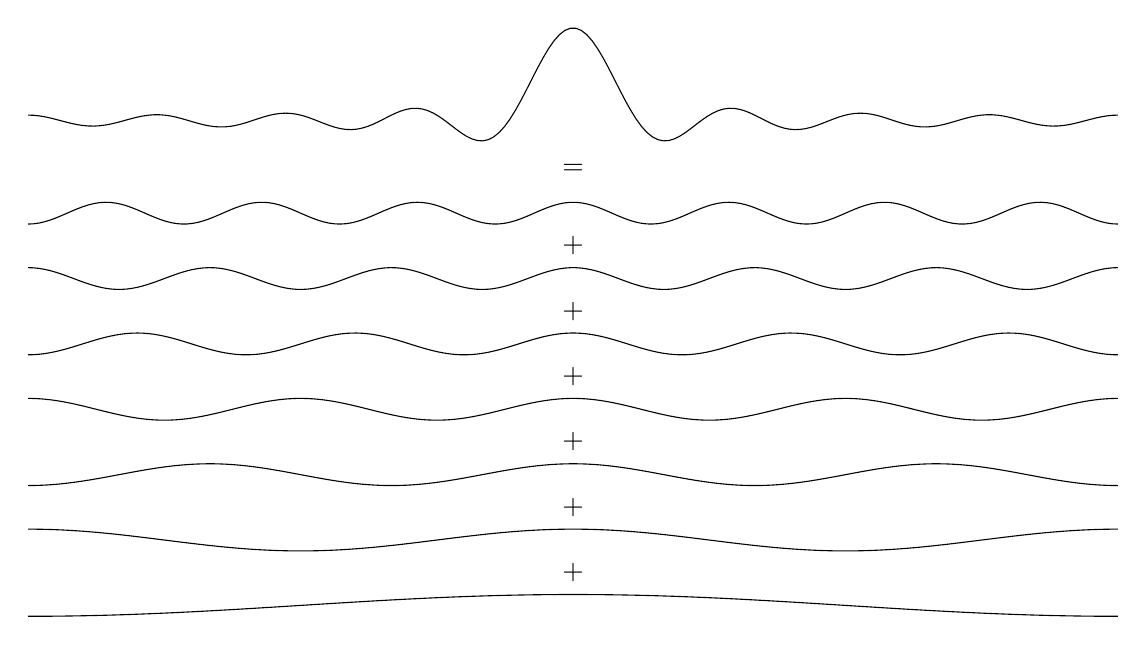
\begin{tikzpicture}
% \begin{pgfinterruptboundingbox}
\begin{axis}[width=1.5\textwidth, height=30em,
%	title={Discrete-time signal},
	axis x line=none,
	axis y line=none
]
\addplot[domain=-100:100,samples=200] {27+
                                       cos( deg(2*3.1415*0.01*0.5*x))+
                                       cos( deg(2*3.1415*0.01*0.5*2*x) )+
                                       cos( deg(2*3.1415*0.01*0.5*3*x) )+
                                       cos( deg(2*3.1415*0.01*0.5*4*x) )+
                                       cos( deg(2*3.1415*0.01*0.5*5*x) )+
                                       cos( deg(2*3.1415*0.01*0.5*6*x) )+
                                       cos( deg(2*3.1415*0.01*0.5*7*x) )+
                                       cos( deg(2*3.1415*0.01*0.5*8*x) ) };

\node at (axis cs:0,22) {$=$};
\node at (axis cs:0,15) {$+$};
\node at (axis cs:0,9) {$+$};
\node at (axis cs:0,3) {$+$};
\node at (axis cs:0,-3) {$+$};
\node at (axis cs:0,-9) {$+$};
\node at (axis cs:0,-15) {$+$};
                                      
\addplot[domain=-100:100,samples=200] {-18+cos( deg(2*3.1415*0.01*0.5*x) ) };
\addplot[domain=-100:100,samples=200] {-12+cos( deg(2*3.1415*0.01*0.5*2*x) ) };
\addplot[domain=-100:100,samples=200] {-6+cos( deg(2*3.1415*0.01*0.5*3*x) ) };
\addplot[domain=-100:100,samples=200] {0+cos( deg(2*3.1415*0.01*0.5*4*x) ) };
\addplot[domain=-100:100,samples=200] {6+cos( deg(2*3.1415*0.01*0.5*5*x) ) };
\addplot[domain=-100:100,samples=200] {12+cos( deg(2*3.1415*0.01*0.5*6*x) ) };
\addplot[domain=-100:100,samples=200] {18+cos( deg(2*3.1415*0.01*0.5*7*x) ) };
\end{axis}
%\end{pgfinterruptboundingbox}
%\draw[use as bounding box] ([xshift=0cm,yshift=0cm]current axis.south west) 
%    rectangle ([xshift=0cm,yshift=0cm]current axis.north east);
\end{tikzpicture}
}
}

\title[Signal processing]{%
  \setlength{\parindent}{0pt}%
  Signal processing\par \vspace{1cm}
    \usebox{\titleimage}
  }
  
\author{Juha Vierinen, J\o{}rn Olav Jensen}
\date{Fall 2022}


\begin{document}
\frontmatter
%----------------------------------------------------------------------------------------
%	EPIGRAPH
%----------------------------------------------------------------------------------------

%----------------------------------------------------------------------------------------

\maketitle % Print the title page

%----------------------------------------------------------------------------------------
%	COPYRIGHT PAGE
%----------------------------------------------------------------------------------------

\newpage
\begin{fullwidth}
~\vfill
\thispagestyle{empty}
\setlength{\parindent}{0pt}
\setlength{\parskip}{\baselineskip}
Copyright \copyright\ \the\year\ \thanklessauthor

\par\smallcaps{Published as lecture notes.}% \thanklesspublisher}

\par\smallcaps{\url{http://kaira.uit.no/fys2006}}

%\par License information.\index{license}

\par\textit{\monthyear}
\end{fullwidth}

%----------------------------------------------------------------------------------------

\tableofcontents % Print the table of contents

%----------------------------------------------------------------------------------------

%\listoffigures % Print a list of figures

%----------------------------------------------------------------------------------------

%\listoftables % Print a list of tables

%\lstlistoflistings

%----------------------------------------------------------------------------------------
%	DEDICATION PAGE
%----------------------------------------------------------------------------------------

%\if 0
\cleardoublepage
~\vfill
\begin{doublespace}
\noindent\fontsize{10}{10}\selectfont\itshape
\nohyphenation
I'd like to thank the following people\sidenote{or their aliases, as
some may have chosen not to use their real names when participating in
the course commentary on Perusall.} for corrections and suggestions
that have improved these lecture notes over the years: Björn
Gustavsson, Patrick Guio,
%(2020)
Mikkel Isak Gaup, Adrian Sletten$^{32}$,
Rikke Bjarnesen Andresen, Jostein Henriksen$^7$, Daniel Nordahl Jørgensen,
Ivan Mikheev, Oskar Marthinussen, Iver Martinsen, Marit Breimo, Sigurd
Haugse, Ragnar Helgaas, Sondre Thomassen, Sofie Svenøe, Sigurd Yngvar
Ekern, Vetle Hofsøy-Woie, Øyvind Alexander Larssen, Erlend
Thorkildsen, Amalie Gjelsvik, Tommy Ryan, Eivind Dragset, Attiqa
Abrar, Daniel Breiland Teigen, Sigrid Holm, Åse Fauske, Yvonne
Johansen, Frank Martin Fossland, Runar Folke-Olsen, Morten Paulsen,
Teodor Skotnes,
%(2021)
Martin Stave$^{16}$, Kristine Rein$^{3}$, Anna Odh$^{2}$, Vegar
Einarsen$^{1}$, Christian Salomonsen$^{5}$, Jonas Riise$^{1}$, Jørn
Jensen$^{63}$, Anton Zyranov$^{1}$, Nikolai Anfeltmo$^{1}$, Håkon
Johansen$^{10}$, Kian Sadeghi$^{3}$, Johannes Bjørnhaug$^{2}$, Ines
Seeliger$^{2}$, Dana King$^{3}$, Emil Jettli$^{1}$, Sigurd
Hanssen$^{1}$, Liza Liz$^{1}$, Sebastian Iversen$^{1}$, Daniel
Johansen$^{1}$, Tobias W. Tobiassen$^{1}$, and Johanna Mankova
Buseth$^{1}$. I'd also like to thank countless others whose names I
have forgotten to mention. A number indicates how many corrections were
found by each person. This is a very rough estimate based on my
somewhat incomplete bookkeeping, which I only started midway through
this project. All mistakes are purely mine.
\end{doublespace}
\vfill
\vfill
%\fi





\cleardoublepage


%----------------------------------------------------------------------------------------
%	This is where the bulk of the content is
%       Use \if 0 and \fi to comment out the parts that you don't need to compile
%----------------------------------------------------------------------------------------
\ifSpIntro
\chapter{Introduction}
\newthought{Many aspects of the life of a modern human} depend on the theory of
\index{signal processing}{signal processing}. Here are a few examples.
When you are listening to a digital audio recording of music,
displaying an image on your computer, or using a wireless internet connection,
you are relying on mathematical concepts that are taught in a basic course on signal processing.
These same concepts are encountered when, e.g., solving differential equations,
applying deep learning techniques, measuring the gravitational wave signature of
colliding neutron stars with a laser interferometer, or making an image of a black hole
using a worldwide network of radio telescopes.
The theory of \emph{\index{signals and systems}{signals and systems}} is a collection of
applied mathematical tools that have important applications in science, technology, and engineering.
The term signal processing and the terminology of signal processing have origins in electrical engineering.

\begin{marginfigure}[-4.2cm]
	\begin{center}
		\includegraphics[width=\textwidth]{ch01/figures/prism.png}
	\end{center}
	\caption{Light can be viewed as a superposition of electromagnetic waves
		with different amplitudes, phases, and frequencies. This can be
		investigated in practice with the help of a prism or a diffraction
		grating. My hope is that after taking this course, you will
		metaphorically be able to ``see'' arbitrary signals as a sum of
		periodic harmonic functions or \emph{spectral components}.}
	\label{fig:prism}
\end{marginfigure}

\newthought{Let's look more closely at the audio example}. When you
listen to a recording of music, you are probably relying on a digital
representation of the acoustic signal that
is \emph{\index{compression}{compressed}}. With the help of signal
processing mathematics, the audio signal is encoded in a special way,
which allows the size of the file to be greatly reduced. This lowers
the minimum internet speed required to stream the audio without
annoying interruptions and allows 10 to 100 times more audio files to
be stored on a digital storage device than without compression.

\index{compression algorithm}{Audio compression algorithms}
often rely on the fact that the \emph{frequency domain}
or \emph{spectral} representation of a signal is far more sparse than
the time domain representation. This means that we can approximate the
original audio signal using a sum of a relatively small number of
periodic sinusoidal signal components. Let's say that the original
audio signal is $x(t)$, which represents air pressure as a function of
time. Using the \index{Fourier series}{Fourier series} we can use the
following type of sum to approximate $x(t)$:
\begin{equation}
	x(t) \approx \sum_{n=1}^{N} A_n \sin(\omega_n t + \phi_n) \,\,,
	\label{ch01:eq:fourier_ser}
\end{equation}
with each sinusoidal signal only described by three parameters: an
amplitude $A_n \in \mathbb{R}$, a phase $\phi_n \in \mathbb{R}$, and an angular frequency $\omega_n \in \mathbb{R}$.

\begin{marginfigure}
	\begin{center}
		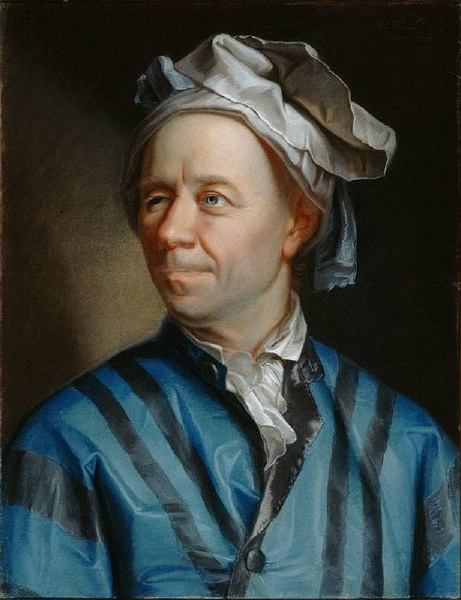
\includegraphics[width=\textwidth]{ch01/figures/euler.jpg}
	\end{center}
	\caption{Leonhard Euler. Credit: Jakob Handmann (1753)}
	\label{fig:euler_pic}
\end{marginfigure}

If the value of $N$ in Equation \ref{ch01:eq:fourier_ser} is
sufficiently small, then the amount of information required to
represent the audio signal as a sum of sinusoids can be significantly
less than what would be required if the signal was just sampled with a
fixed sample spacing and the amplitude of the waveform at each sampled
point would be stored.

Here's an example. Let's say that you want to store 1024
\emph{samples}\sidenote{One sample is a number representing the audio signal amplitude at one instant of time} of
audio signal. With the signal represented using 44100 samples per second,
this would be approximately 0.023 seconds of signal. You'd need to
store 1024 numbers without compression. With 16 bits per sample, this
audio signal would require 16384 bits of storage space. However, if
the signal is sufficiently well represented using $N=10$ sinusoidal
components, you'd only need to store 30 numbers to retain the
information about the phase, amplitude and frequency of each
sinusoidal component. This is only approximately 3\% of the original
data, or 480 bits of storage space at 16 bits per number\sidenote{One
	"bit" of information is an answer to a yes or no question. One bit
	would allow you to say that a number is either 0 or 1. A two bit
	signal would allow you to say that a number is either 0, 1, 2, or 3.}.

Most of the videos, images, and music that you access over the
internet is compressed in this manner. Without spectral compression
techniques, the internet would most likely need to have at least 10
times more capacity than it currently has, in order to be able to
provide us with the same amount of entertainment. For example,
the \index{MP3}{MP3} audio compression standard and
the \index{JPEG}{JPEG} image compression standard both utilize spectral
compression methods.

%This is also the reason why sometimes the audio
%in an online meeting sounds a bit ``robotic'' when you have a very
%poor internet connection -- it is represented with only a small number
%of sinusoidal components. 

\newthought{We often use more general complex-valued sinusoidal functions}
instead of real-valued ones when describing the theory of signal
processing. These are defined as follows:
\begin{equation}
	A e^{i\phi }e^{i\omega t} = A[\cos(\omega t+\phi) + i\sin(\omega
			t+\phi)] \,\,.
	\label{ch01:eq:euler}
\end{equation}
Just like a real-valued sinusoid, the complex sinusoid is also
represented using an amplitude $A \in \mathbb{R}$, phase
$\phi \in \mathbb{R}$, and angular frequency $\omega \in \mathbb{R}$. Note
that the above equation is just an application of Euler's
formula\sidenote[][1cm]{The famous physicist \index{Richard
		Feynman}{Richard Feynman} had this to say about \index{Euler's
		formula}{Euler's formula}: ``We summarize with this, the most
	remarkable formula in mathematics. This is our jewel.'' (Feynman
	Lectures on Physics, Vol I). He had clearly benefited greatly from
	this formula.}, which is probably the most frequently occurring
equation in signal processing. If you master this equation, you'll have covered most of the mathematical prerequisites for this course!


If you are not familiar with complex algebra,
Equation \ref{ch01:eq:euler} might at first seem intractable. But
don't worry. If you have a hard time grasping the function $A e^{i\phi
		}e^{i\omega t}$, just think of it as a periodic function like
$A\cos(\omega t + \phi)$, but with a real and imaginary sinusoidal
component. The reason for using the complex sinusoidal signal instead
of the real-valued one is that most of the mathematical calculations
are greatly simplified.

\begin{marginfigure}
	\begin{center}
		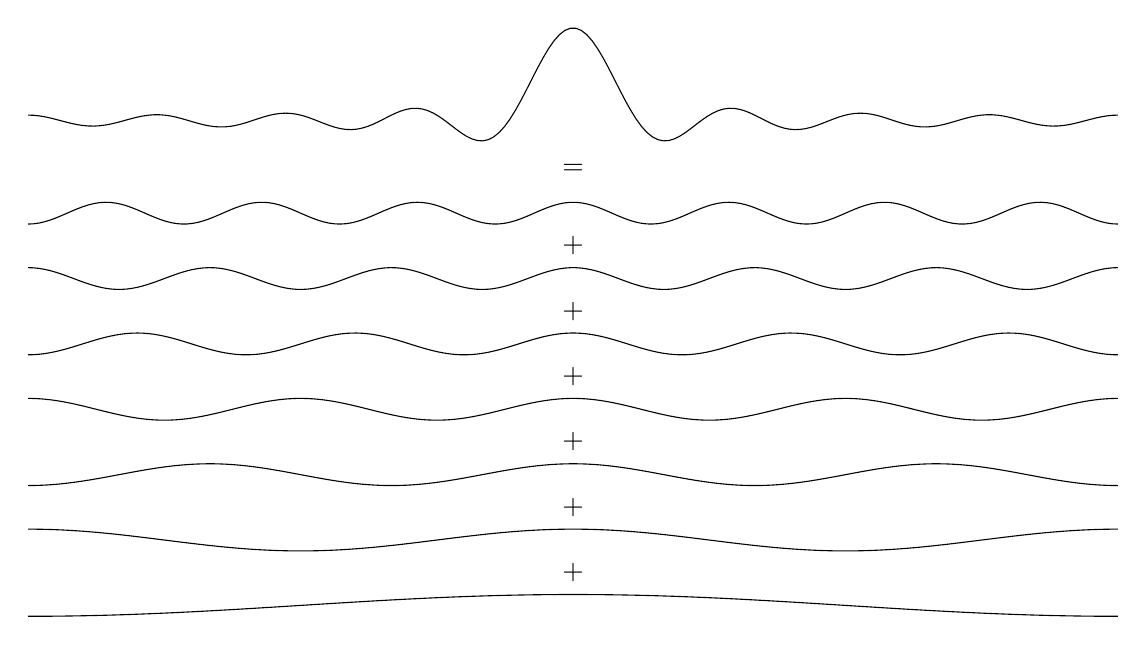
\begin{tikzpicture}
			% \begin{pgfinterruptboundingbox}
			\begin{axis}[width=1.5\textwidth, height=30em,
					%	title={Discrete-time signal},
					axis x line=none,
					axis y line=none
				]
				\addplot[domain=-100:100,samples=200] {27+
					cos( deg(2*3.1415*0.01*0.5*x))+
					cos( deg(2*3.1415*0.01*0.5*2*x) )+
					cos( deg(2*3.1415*0.01*0.5*3*x) )+
					cos( deg(2*3.1415*0.01*0.5*4*x) )+
					cos( deg(2*3.1415*0.01*0.5*5*x) )+
					cos( deg(2*3.1415*0.01*0.5*6*x) )+
					cos( deg(2*3.1415*0.01*0.5*7*x) )+
					cos( deg(2*3.1415*0.01*0.5*8*x) ) };

				\node at (axis cs:0,22) {$=$};
				\node at (axis cs:0,15) {$+$};
				\node at (axis cs:0,9) {$+$};
				\node at (axis cs:0,3) {$+$};
				\node at (axis cs:0,-3) {$+$};
				\node at (axis cs:0,-9) {$+$};
				\node at (axis cs:0,-15) {$+$};

				\addplot[domain=-100:100,samples=200] {-18+cos( deg(2*3.1415*0.01*0.5*x) ) };
				\addplot[domain=-100:100,samples=200] {-12+cos( deg(2*3.1415*0.01*0.5*2*x) ) };
				\addplot[domain=-100:100,samples=200] {-6+cos( deg(2*3.1415*0.01*0.5*3*x) ) };
				\addplot[domain=-100:100,samples=200] {0+cos( deg(2*3.1415*0.01*0.5*4*x) ) };
				\addplot[domain=-100:100,samples=200] {6+cos( deg(2*3.1415*0.01*0.5*5*x) ) };
				\addplot[domain=-100:100,samples=200] {12+cos( deg(2*3.1415*0.01*0.5*6*x) ) };
				\addplot[domain=-100:100,samples=200] {18+cos( deg(2*3.1415*0.01*0.5*7*x) ) };
			\end{axis}
			%\end{pgfinterruptboundingbox}
			%\draw[use as bounding box] ([xshift=0cm,yshift=0cm]current axis.south west) 
			%    rectangle ([xshift=0cm,yshift=0cm]current axis.north east);
		\end{tikzpicture}
	\end{center}
	\caption{Spectral decomposition of a narrow pulse that consists of seven sinusoidal signals.}
	\label{fig:dtfig0}
\end{marginfigure}

\begin{marginfigure}
	\begin{center}
		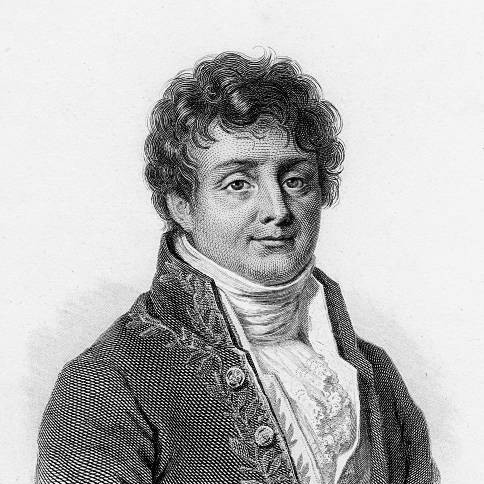
\includegraphics[width=\textwidth]{ch01/figures/fourier_head.jpg}
	\end{center}
	\caption{Jean-Baptiste Joseph Fourier}
	\label{fig:joe_fourier}
\end{marginfigure}

\newthought{A general frequency domain decomposition of signals is known as the
	\emph{\index{Fourier transform}{Fourier transform}}}.
This is just an extended version of the sum of sinusoidal signals given in Equation \ref{ch01:eq:fourier_ser}. The
reverse and forward Fourier transforms allow transforming a signal
between a time domain and a frequency domain representation:
\begin{align}
	x(t)            & = \frac{1}{2\pi}\int_{-\infty}^{\infty} \hat{x}(\omega) e^{i\omega t} d\omega \\
	\hat{x}(\omega) & = \int_{-\infty}^{\infty} x(t) e^{-i\omega t} dt \,\,.
\end{align}
The Fourier transform allows nearly any function to be expressed as an
infinite sum of complex sinusoidal functions, or in other words, an
integral. This is one of the main theoretical foundations of signal
processing. In this equation, the term $x(t)$ is the time domain
representation of the signal, and $\hat{x}(\omega)$ is the frequency
domain representation of the signal. The function $\hat{x}(\omega)$
simply tells you what is the phase $\phi$ and amplitude $A$ of
each spectral component of the signal, assuming that it consists of
infinitely many sinusoidal components.

Figure \ref{fig:dtfig0} shows a sketch of the basic idea behind the
Fourier decomposition of signals. By adding together the seven
individual sinusoidal signals on the bottom of the figure, we obtain
the more pulse-like signal shown on the top of the figure. Conversely,
the pulse-like signal on the top can therefore be decomposed into
seven sinusoidal signals. This is in essence the idea behind the
forward and reverse Fourier transform. Had we continued to sum
together higher and higher frequency sinusoidal signals in the same
manner, we would have ended up with an infinitely narrow spike
$\delta(t)$, which is called the Dirac delta function. This special
function has many important theoretical uses in signal
processing.

The Fourier transform is named after Jean-Baptiste Joseph Fourier, who
is shown in Figure \ref{fig:joe_fourier}. He was the first to come up
with the idea of expressing a function as a sum of sinusoidal signals,
or in other words, spectral components. This occurred in the 1820s
while he was studying heat conduction. Using sinusoidal valued
spectral components to represent the distribution of heat within a
body allowed him to analytically solve the heat equation, because
solving differential equations is relatively straightforward for
sinusoidal functions. Even though this brilliant mathematical
discovery occurred 200 years ago, we are still coming up with new ways
to apply it\sidenote{For example, your smartphone relies on the Fourier
	transform in several ways for enabling transfer of data over
	radio waves, and for storing pictures, videos, and audio
	files.}. I would say that the ability to divide nearly any function you
encounter into a superposition of simple elementary sinusoidal waves
(the concept of the Fourier transform) is the most useful idea you
will learn from a basic course on signal processing.

If you are not yet completely sure what the equations in this chapter
mean, that is perfectly fine. Learning what the equations are and how
to apply them in practice is the purpose of this course. If you are
already familiar with complex sinusoidal signals and the Fourier
transform, then you may be able to skip much of the introductory
material and spend more time on the application examples.

%% That is it for now. Thank you for listening.
%% The next lecture will discuss how to setup a python programming environment for doing signal processing.
%% The animation that I'm concluding with is a Fourier transform of Jean-Baptiste Joseph Fourier.
%% I have decomposed his figure into two dimensional plane waves, or two dimensional sinusoids.

%% I am showing you what the Fourier series approximation of the picture looks like using a sum of the N largest
%% amplitude spectral components of of the picture of Joseph Fourier looks like. As you can see, when we add more spectral
%% components to the Fourier series approximation, the image quality improves.
%% As you might guess, this is the basic principle behind spectral image compression techniques, such as the JPEG standard.
%% Anyway, see you next time.

%% Here are some other examples of signal processing topics where you
%% will encounter the Fourier transform. You will encounter
%% it when analyzing the properties of filters that modify signals, when
%% applying a filter on a signal, or when searching for solutions of
%% differential equations. The fundamental theorem of discretizing
%% signals, the \emph{Shannon-Nyquist theorem}, relies on the Fourier
%% transform. A two dimensional variant of the Fourier transform is a
%% fundamental part of the theory for making a radio astronomical images
%% using a spatially distributed network of radio telescopes, but it is
%% also often used in image compression.

%Where can one apply the elementary concepts of signal processing
%concepts? Data science, machine learning, differential equations,
%electrical engineering, measurement modeling, telecommunications,
%spectral analysis of measurements, are all examples of application
%areas where basic signal processing concepts are useful.

\if 0
	\begin{marginfigure}[1.0cm]
		\begin{center}
			\includegraphics[width=\textwidth]{up.jpg}
		\end{center}
		\caption{Arecibo Observatory radio telescope measurements of the first pulsar ever discovered, CP1919. The vertical axis represents received signal power and the horizontal axis represents time. Successive pulses of the pulsar are shown on each row. The figure is originally from “Radio Observations of the Pulse Profiles and Dispersion Measures of Twelve Pulsars,” by Harold D. Craft, Jr. (September
			1970). Signal processing is an important part of practical radio astronomy.}
	\end{marginfigure}
\fi



%In many cases, these two categories of signal processing are very
%closely related. For example, the \index{Shannon-Nyquist sampling
%theorem}{Shannon-Nyquist sampling theorem} provides the fundamental
%limits on the information content of a discrete-time signal. It does so by showing
% how a continuous-time signal can be reconstructed perfectly from a
%discrete-time signal, as long as certain conditions on the sample-rate
%and spectral occupancy of the continuous-time signal signal are met.

%The study of signals and systems has evolved significantly over
%time. While many of the fundamental concepts, such as
%the \index{Fourier transform}{Fourier transform} or the Shannon
%sampling theorem, are unchanged and will remain the fundamental
%pillars of signal processing, the exponential increase in the speed of
%general purpose computers has meant that more and more signal
%processing is digital and discrete-time instead of analog.

%Nowadays, digital signal processing is performed mostly with general
%purpose computers and implemented with software, instead of dedicated
%custom digital processing hardware. We will therefore devote much time
%to discrete-time signals and systems and focus on software aspects of
%signal processing in the practical application examples.

%Still, there are always some things that will always remain analog, so
%we cannot completely avoid continuous-time signals. The real world
%itself is continuous, or at least most of us think it is. We therefore
%will cover the theoretical aspects of continuous-time signal
%processing. The continuous-time theory also forms the theoretical
%foundation for much of the discrete-time signal processing.

%However, we will not go into great detail on analog signal
%processing, as this is a topic better suited for a course on circuit
%analysis or radio engineering. We will also not cover any advanced
%continuous-time concepts, such as the Laplace transform, which is a topic perhaps better suited for a course on differential equations.


\begin{marginfigure}%
	\begin{center}
		\begin{tikzpicture}
			\begin{axis}[width=\textwidth,
					xticklabels=\empty,
					yticklabels=\empty,
					xmin=-1.5,xmax=6,
					axis x line=bottom,
					axis y line=left,
					xlabel={Independent variable $t$},
					xlabel style={below},
					ylabel={Dependent variable $x(t)$},
					xlabel style={ yshift = { 1em } },
					ylabel style={ yshift = { -2.2em } }
				]
				\addplot[draw=blue,domain=-1:7,samples=150] {(x>0)*exp(-x)};
			\end{axis}
		\end{tikzpicture}
	\end{center}
	\caption{Continuous-time signal.}
	\label{fig:ctfig_intro}
\end{marginfigure}

\begin{marginfigure}%
	\begin{center}
		\begin{tikzpicture}
			\begin{axis}[width=\textwidth,
					%	title={Discrete-time signal},
					xticklabels=\empty,
					yticklabels=\empty,
					xmin=-1.5,xmax=6,
					axis x line=bottom,
					axis y line=left,
					xlabel={Independent variable $n$},
					xlabel style={below},
					ylabel={Dependent variable $x[n]$},
					xlabel style={ yshift = { 1em } },
					ylabel style={ yshift = { -2.2em } }
				]
				\addplot+[ycomb,domain=-1:5,samples=15] {(x>0)*exp(-x)};
			\end{axis}
		\end{tikzpicture}
	\end{center}
	\caption{Discrete-time signal.}
	\label{fig:dtfig_intro}
\end{marginfigure}

\newthought{Signal processing is an interdisciplinary field, where mathematics,
	physics, computer science, and engineering intersect}. The theoretical
aspects of signal processing are essentially just applied mathematics,
which often have already been introduced hundreds of years
ago. However, applying the theory to solve real world problems
involves programming or building electrical circuits. This aspect
of signal processing is technology driven, and is continuously
evolving as technology advances. This course will go through the theoretical foundations of signal processing without trying to skip over any important theoretical concepts, but the main emphasis will be in how these concepts can be applied to real world problems.

These lecture notes aim to teach theoretical and applied aspects of signal
processing through mathematical derivations and programming
examples. The mathematics we will use is not rigorous or generalized
in a sense that it would appeal to a mathematician. Similarly, we will
not emphasize aspects of proper software engineering. Instead, the aim
is to provide programming examples that are as simple and as easy to
understand as possible.

My hope is that these notes will take an approach to signal processing
which is appealing to an undergraduate level physics or engineering
student. I do not expect you to have ever encountered a Fourier
transform before, to be familiar with complex algebra, or even be
proficient in programming.

It is natural to divide the topic of signal processing into two main
categories: \emph{\index{continuous-time}{continuous-time}}
and \emph{\index{discrete-time}{discrete-time}}. The former deals with
signals that are continuous functions. The latter deals with signals
that are sequences of numbers, which is more natural for signals that
reside on digital computers and that are used for digital signal
processing. The latter type of signal processing has gained in
importance for quite a long time due to the exponential increase in
computing and storage capacity, which has made it possible to perform
more and more signal processing tasks digitally. The theory for
continuous-time signals lays the theoretical foundation for also the
discrete-time signal processing, so it is still important to teach
this part.

\newthought{This compendium covers} the topics in the syllabus of the
undergraduate signal processing course ``FYS-2006'' held at University
of Troms\o{}. While many other universities will have a separate
``signals and systems'' course that covers continuous-time signals,
and a separate course dedicated to ``digital signal processing'', this
course combines both topics in one course.

These lecture notes are complete in terms of the topics that are
covered in the course ``FYS-2006''. You are not required to obtain any
additional reading material. The reason why I went through the trouble
of typing out these notes is that there currently are no signal
processing textbooks that cover continuous-time and discrete-time
signal processing, and use the Python programming language for
examples. If you wish to deepen your knowledge, there are several
published textbooks that you can use to complement this material. One
book that I recommend is ``Applied Digital Signal Processing: Theory
and Practice'' by D. G. Manolakis and V. K. Ingle.


%\footnote{For some bizarre reason, the University recently
% changed
%its name to \emph{UiT - The Arctic University of Norway}, where UiT is
%a Norwegian language acronym for University of Troms\o{}. Why there is
%an unexplained acronym in the name of the university, why the word
%university is repeated twice, and why there are two different place
%names is a mystery to many of us working at the university. Some even
%insist on continuing the use of the old name, which further increases
%confusion related to the name of the institution.}.


\newthought{You might be asking yourself: why should I learn about signal processing?}
This may be in the minds of, especially those for who have this as a mandatory course,
and this is the primary reason that you are attending it.
I believe that the elementary concepts taught in a basic course on this topic will provide
you with the tools to be a good scientist. You will encounter the mathematical tools
introduced in this course throughout science, technology, and engineering, where knowledge
of these tools can often be seen as prerequisite background knowledge
that allows you to understand more advanced concepts.

Perhaps the most powerful practical tool you will learn during this course
is the Fast Fourier Transform (FFT), which is a specific algorithm used to compute a
discrete Fourier transformation. It will allow you to perform a wide range of different
calculations efficiently, using techniques that are not trivial unless you understand the
basic concepts of signal processing. The FFT algorithm can be used e.g., for spectral analysis,
evaluation of a convolution operation, to efficiently solve certain types of matrix operations,
or to solve differential equations. Any time when processing signals
later on in your life, there is a good chance that you will find the FFT algorithm to be highly useful.

\begin{marginfigure}[1cm]
	\begin{center}
		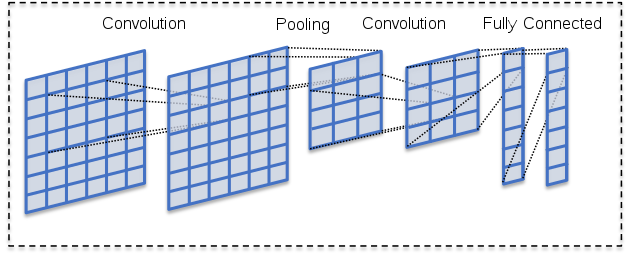
\includegraphics[width=\textwidth]{ch01/figures/cnn.png}
	\end{center}
	\caption{Simplified diagram of a convolutional neural network, where a convolution operation is one of the fundamental components. Figure adapted from \citep{maier2019gentle}.}
	\label{fig:cnn}
\end{marginfigure}

If you go on to work with e.g. machine learning, this course will teach you the concept of convolution,
which is a mathematical operation that describes an arbitrary linear time-invariant system, and thus plays
a major role in signal processing. You may have heard of convolutional neural networks, right?
This course will not teach you anything about statistics or neural networks, but it will teach you
the concept of a convolution sum, which is often a fundamental
building block of image processing or deep learning algorithms\cite{maier2019gentle}.


% \newthought{Outline of these notes}: The main tool and equation that governs all we do in the course
% is the Fourier transform. We state the transform here, even though it does not make sense (yet!)
% \begin{equation}
% 	\hat{x}(\omega) = \int_{-\infty}^{\infty} x(t)e^{-i\omega t}dt
% 	\label{eq:fourier-transform}
% \end{equation}
% The idea is to learn what this means. Firstly, what is $x(t)$? Well, this is the signal we will
% be "processing", typically being dependent on time. We define what this means in the chapter on 
% signals and systems. Secondly, what is the deal with $e^{-i\omega t}$? 
% This is a complex exponential! Understanding this term will be the focus 
% of the complex algebra chapter and the chapters leading up to the Fourier series. 

\fi

\ifSpPython
\chapter{Python} 
\begin{marginfigure}

\includegraphics[width=\textwidth]{ch02/figures/pylogo.jpg}
\caption{The Python programming language is an open source language that is increasingly popular for data science and signal processing.}
\end{marginfigure}

\newthought{We'll demonstrate various signal processing topics using
  programming} examples. Why \index{Python}{Python} and not some other
language? Here are three justifications:
\begin{itemize}
\item It is free for everyone to use,
\item there are a wide range of efficient numerical libraries available,
\item and Python is nowadays the language that students are most familiar with.
%\item Python has a built-in complex data type, both in single precision and double precision
\end{itemize}

\begin{marginfigure}
\begin{center}
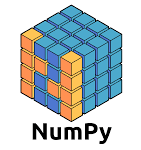
\includegraphics[width=0.5\textwidth]{ch02/figures/numpylogo.png}
\end{center}
\caption{The NumPy package implements a large collection of numerical routines that can be used for signal processing.}
\end{marginfigure}

All the programming examples we'll show in these lecture notes will
support Python 3. We will restrict ourselves to a bare minimum number
of library dependencies. The main libraries you will need are:
\verb|numpy|, \verb|scipy|, and \verb|matplotlib|. These should be
readily available for nearly every operating system.

\begin{marginfigure}
\begin{center}

\includegraphics[width=0.68\textwidth]{ch02/figures/scipy.jpg}
\end{center}
\caption{The Scipy package contains a number of signal processing routines for Python.}
\end{marginfigure}

If you don't know how to obtain Python for your computer, you could
try out the Anaconda distribution of Python. It provides a relatively
complete set of the most commonly used Python modules. You can obtain
this distribution by visiting the anaconda web page:
\url{http://anaconda.org} and downloading the installer for your
platform.

The Anaconda package manager will allow you to install Numpy, Scipy,
and Matplotlib. Anaconda also comes with a Python development
environment as well. If you don't have your mind set on a specific
programming editor yet, you could try out the Spyder development
environment that comes with Anaconda.

\begin{marginfigure}
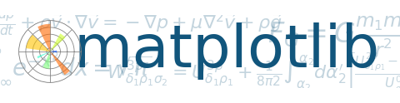
\includegraphics[width=\textwidth]{ch02/figures/matplotlib.png}
\caption{Matplotlib implements a basic plotting routines for Python.}
\end{marginfigure}

If you are using Linux, like I am most of the time, it is
probably easiest to just obtain Python using the system package
manager. On Ubuntu, you would install the necessary packages with the following command:
\begin{lstlisting}[language=sh,caption=Installing Python on Ubuntu Linux,label=lst:linuxinstall]
sudo apt-get install python3 python3-numpy python3-scipy python3-imageio python3-matplotlib ipython3
\end{lstlisting}

\begin{marginfigure}[3cm]

\includegraphics[width=0.68\textwidth]{ch02/figures/analogo.jpg}
\caption{The Anaconda distribution is currently one of the most
  popular distributions of the Python programming language, offering
  nearly all existing open source modules.}
\end{marginfigure}

After installing Python and the required modules, I recommend that you
write a short test program to make sure that all the modules are
installed correctly. To test your Python installation, open up your
programming editor and write a small Python program:
\lstinputlisting[language=Python,caption={\texttt{001\_hello\_world/hello.py}},label=lst:pythonhw]{code/001_hello_world/hello.py}
This test program prints out the standard hello world message, and
uses NumPy and SciPy to print the approximate value of $\pi$. The program then
plots a complex sinusoidal signal with the help of NumPy and
Matplotlib.  If you can run this program without getting any errors,
you are all set. The output should look something like this:

\begin{figure}
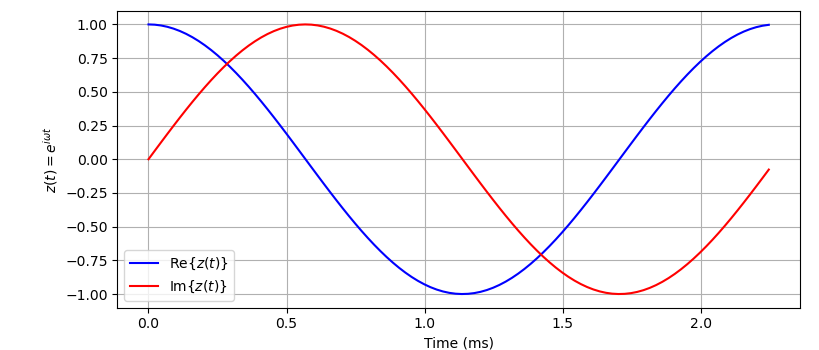
\includegraphics[width=\textwidth]{ch02/figures/testscreen1.png}
\caption{Output of the \texttt{hello.py} test program.}
\end{figure}

\newthought{Code examples} that are spread throughout these lecture
notes can be downloaded from GitHub:
\url{https://github.com/jvierine/signal_processing.git}. The easiest
way to access the code is to just visit this page with your web
browser. In order to download the source code for the examples in
these lecture notes, you can also use git on the command line:
\begin{lstlisting}[language=sh,caption=Obtaining the source code for the programming examples with git,label=lst:download]
git clone https://github.com/jvierine/signal_processing
\end{lstlisting}
\begin{marginfigure}
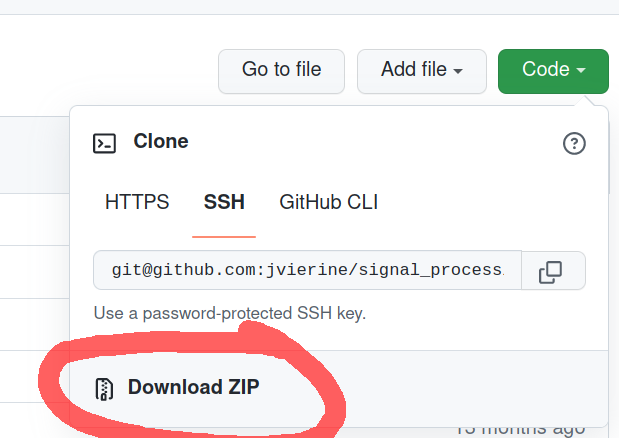
\includegraphics[width=\textwidth]{ch02/figures/downloadgit.png}
\caption{If you are not familiar with git, you can easily download the code from the GitHub webpage as a zip file instead of using the git clone command.}
\end{marginfigure}
If you are using Anaconda, you will have to install git (if you don't
have it already) by typing in
\begin{lstlisting}[language=sh,caption=Obtaining the source code for the programming examples with git,label=lst:download]
  conda install -c anaconda git
\end{lstlisting}
Then you can proceed with the command shown above. 



\begin{marginfigure}

\includegraphics[width=0.68\textwidth]{ch02/figures/gitlogo.png}
\caption{Program examples from these lecture notes are available on GitHub.}
\end{marginfigure}

\newpage
\section{Exercises: Python}

These exercises are intended to get you started with programming with
\emph{\index{Python}{Python}} and the \emph{\index{NumPy}{NumPy}} and
Matplotlib libraries. If you are already familiar with these topics,
you may want to skip these exercises.

\begin{enumerate}
 \item Obtain the source code for the examples by cloning the GitHub
   repository for this course. 
\item The Hello World program shown in Listing \ref{lst:pythonhw} plots a complex sinusoidal signal. 
  \begin{enumerate}[a)]
  \item Go on the NumPy website \url{http://numpy.org}, and find the documentation of the functions included in the package.
  \item Use this documentation to determine what \verb|numpy.arange|, and \verb|numpy.exp| do. 
  \item Modify the code so that it plots a circle on the complex
    plane, by plotting the real part of the complex sinusoidal
    signal \verb|csin| on the x-axis, and the imaginary part on the
    y-axis.
  \item Explain why the real and imaginary component draw a circle on the complex plane.
  \end{enumerate}

\item Use Python to calculate and print out the value of $e^{i \pi} + 1$. Note that $i$ in Python, is denoted
  with \verb|1j|.
  
\item The use of built-in Numpy functions will let you program
  efficiently. The program shown in Listing \ref{lst:exercise002}
  demonstrates the use of Numpy functions to evaluate the Mandelbrot
  set with a slight twist.

\lstinputlisting[language=Python,caption={\texttt{001\_hello\_world/mystery.py}},label=lst:exercise002]{code/001_hello_world/mystery.py}

\begin{enumerate}[a)]
  \item Run the program shown in Listing \ref{lst:exercise002}. You
    	should see a plot like the one shown in Figure \ref{fig:mandelbrot}.
  \item Describe what each line of the program does by adding comments to the code.
  \item It is possible to specify the data type of any NumPy array
      	using the \verb|dtype| attribute? There are two complex valued
      	datatypes available in NumPy: \verb|complex64| and \verb|complex128|. 
      	What are the pros and cons of using the \verb|complex64| datatype 
      	instead of the \verb|complex128| datatype? 
\end{enumerate}


\begin{figure}
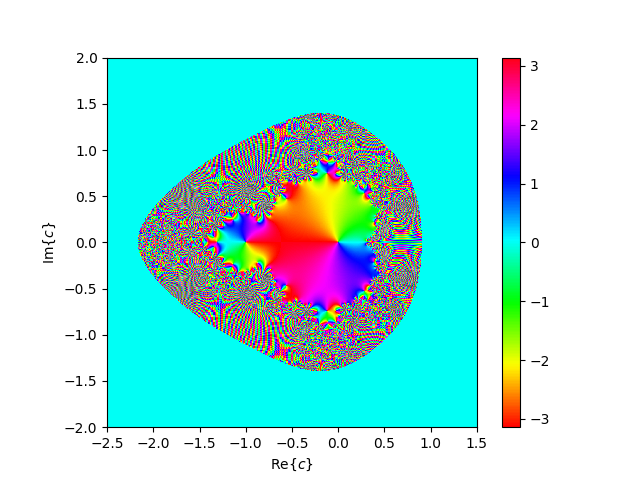
\includegraphics[width=0.9\textwidth]{ch02/figures/mystery.png}
\caption{The Mandelbrot set example demonstrates the use of NumPy array functions and complex numbers. The plot
  shows the phase of complex number $z_{12}$ after 12 iterations of
  $z_{n+1} \leftarrow z_n^2 + c$, starting with $z_0 = 0$.}
\label{fig:mandelbrot}
\end{figure}



\end{enumerate}

 \ifSpExerciseSol
   \newpage
\section{Suggested solutions: Python}


\begin{enumerate}
\item If you use Linux type: \verb|git clone https://github.com/jvierine/signal_processing| in the terminal and hit enter.
On Windows and MacOS, I don't know...? Google it, I guess. You can also just download it directly from GitHub.

\item 
\begin{enumerate}[a)]
\item Go here \url{http://numpy.org} to read documentation. 
\item Reading the documentation you'll find that \verb|n.arange| creates a NumPy array 
      of evenly spaced numbers from 0 to the provided number minus 1. In the case of the code here, 
      the \verb|n.arange| function will sequence the numbers from 0 to 99 and return a NumPy array containing these numbers. 
      See documentation: \url{https://numpy.org/doc/stable/reference/generated/numpy.arange.html}.
      The documentation for \verb|n.exp| can be found here \url{https://numpy.org/doc/stable/reference/generated/numpy.exp.html}.
      The function simply computes $e^{x}$, where $x$ can be real or complex, or even a NumPy array. If so, a NumPy array is returned. 
\item Listing \ref{circle_plot} now plots a circle. 
\lstinputlisting[language=Python,caption=Code is modified to plot a circle,label=circle_plot,linerange={0-24}]{ch02/code/ex2_2.py}

\begin{marginfigure}
%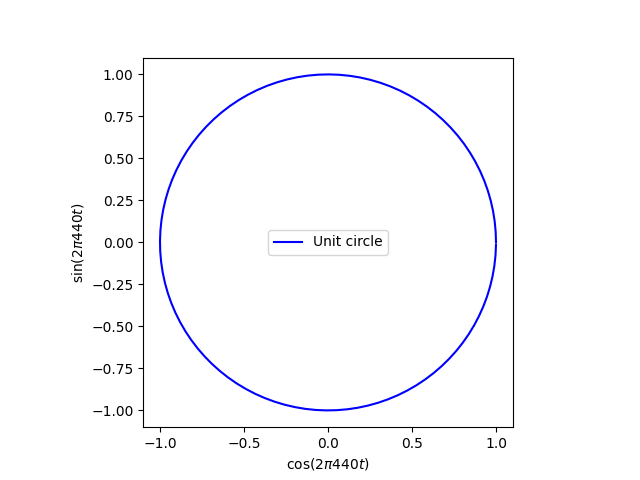
\includegraphics[width=6.5cm,height=6.0cm]{ch02/figures/circle_plot.png}
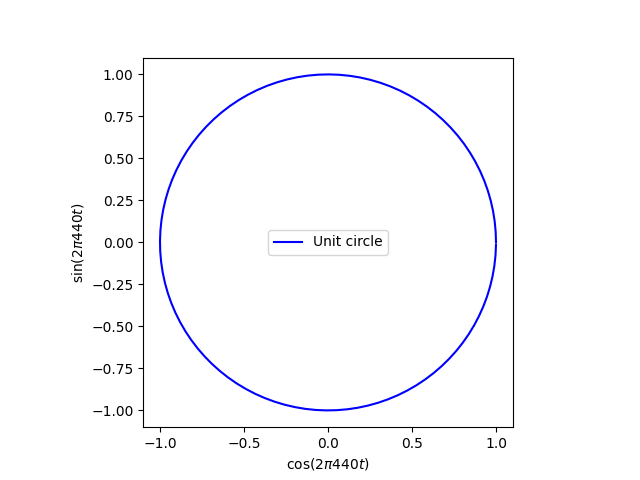
\includegraphics[width=\textwidth]{ch02/figures/circle_plot.png}
\caption{Output of Listing \ref{circle_plot}}
\end{marginfigure}

\item The unit circle can be described by the equation $x^{2} + y^{2} = 1$, which is satisfied by $x=\cos(t)$ and $y =\sin(t)$. 
\end{enumerate}


\item Listing \ref{ipi} shows how to compute and print $e^{i\pi}+1$ in Python. The resulting output is \verb|1.2246467991473532e-16j|, which is not zero.
The reason for this is due to floating point errors. The value is very close to 0, but not exactly 0. 

\lstinputlisting[language=Python,caption=Computing $e^{i\pi}+1$, label = ipi]{ch02/code/ex2_3.py}

\item The following is a solution for Exercise 4.

\begin{enumerate}[a)]
\item Running the code generates the plot shown in the exercise. 

\item Adding comments in Python can be done using \verb|#|, Listing \ref{comments_on_code} shows some comments.
\lstinputlisting[language=Python,caption=Commented Python code, label=comments_on_code]{ch02/code/ex2_4.py}

\item Yes, one can specify the data type of a NumPy array. The data types supported can be found in the documentation. 
These include: \verb|complex64|, \verb|complex128|, \verb|float32|, \verb|int32|, among others. 
Pros and cons with the \verb|complex64| and \verb|complex128| include: size and accuracy. The \verb|complex64|
takes less memory, but is less accurate, while \verb|complex128| can store more accurate numbers, but takes more memory.

\end{enumerate}





\end{enumerate}

 \fi
\fi

\ifSpComplex
\chapter{Complex Algebra}
\newthought{Complex algebra is found throughout signal processing}. In this chapter, we'll briefly review the basics of this topic. Of primary importance is \index{Euler's formula}{Euler's formula}, which will be used extensively throughout this course.

\begin{marginfigure}
\begin{center}
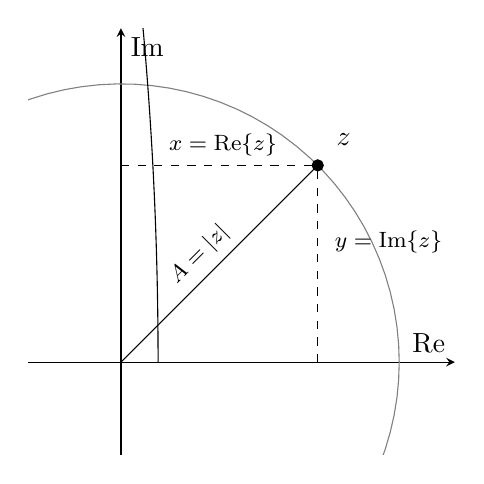
\begin{tikzpicture}
	\begin{axis}[axis equal, ymin=-0.5,xmin=-0.5,ymax=1.8,xmax=1.8,  ticks=none,
    xlabel=$\mathrm{Re}$,
    ylabel=$\mathrm{Im}$, axis lines = center, width=7cm, height=7cm]
	
    \addplot [gray,domain=0:2*pi,samples=100]({1.5*cos(deg(x))},{1.5*sin(deg(x))});
    
    \addplot [black, mark = *] coordinates {( {1.5*cos(45)}, {1.5*sin(45)} )} {};   
 %   \addplot [black, mark = *] coordinates {( {1.5*cos(-60)}, {1.5*sin(-60)} )} {};   

\addplot [black] coordinates { (0,0) ( {1.5*cos(45)}, {1.5*sin(45)} ) };
    
    \addplot [dashed,black] coordinates { ({1.5*cos(45)},0) ( {1.5*cos(45)}, {1.5*sin(45)} ) };
    
    \addplot [dashed,black] coordinates { (0,{1.5*sin(45)}) ( {1.5*cos(45)}, {1.5*sin(45)} ) };

  \draw[draw=black] (axis cs:0.2,0) arc [radius={transformdirectionx(0.2)},start angle=0,end angle=45]
  node[midway,right,inner sep=3pt,font={\footnotesize}]{$\theta=\angle z$};

 \node at (axis cs:0.55,1.06) [above, font={\footnotesize}]{$x=\mathrm{Re}\{z\}$};
 
 \node at (axis cs:1.1,0.65) [right, font={\footnotesize}]{$y=\mathrm{Im}\{z\}$}; 
 
 \node at (axis cs:1.2,1.2) {$z$};

 \node at (axis cs:0.5,0.5) [above,rotate=45,font={\footnotesize}]{$A=|z|$};
\end{axis}
\end{tikzpicture}
\end{center}
\caption{The polar representation of a complex number $z=x+iy =Ae^{i\theta}$.}
\label{fig:polar_euler}
\end{marginfigure}

\if 0
\begin{marginfigure}

\begin{center}
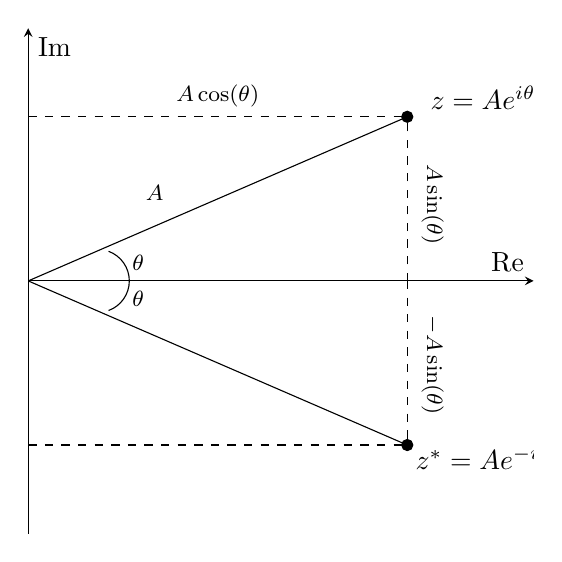
\begin{tikzpicture}
	\begin{axis}[
        ymin=-2.0,
        xmin=0.0,
        ymax=2.0,
        xmax=1.0,
        ticks=none,
        xlabel=$\mathrm{Re}$,
        ylabel=$\mathrm{Im}$,
        axis lines = center,
        width=8cm, height=8cm]
    \addplot [black, mark = *] coordinates {( {1.5*cos(60)}, {1.5*sin(60)} )} {};   
    \addplot [black, mark = *] coordinates {( {1.5*cos(-60)}, {1.5*sin(-60)} )} {};   

\addplot [black] coordinates { (0,0) ( {1.5*cos(60)}, {1.5*sin(60)} ) };
    \addplot [dashed,black] coordinates { ({1.5*cos(60)},0) ( {1.5*cos(60)}, {1.5*sin(60)} ) };
    \addplot [dashed,black] coordinates { (0,{1.5*sin(60)}) ( {1.5*cos(60)}, {1.5*sin(60)} ) };

\addplot [black] coordinates { (0,0) ( {1.5*cos(-60)}, {1.5*sin(-60)} ) };
    \addplot [dashed,black] coordinates { ({1.5*cos(-60)},0) ( {1.5*cos(-60)}, {1.5*sin(-60)} ) };
    \addplot [dashed,black] coordinates { (0,{1.5*sin(-60)}) ( {1.5*cos(-60)}, {1.5*sin(-60)} ) };

%  \draw [black,-] (0,0) arc [radius=0.5,start angle=0,end angle=60];
  \draw[draw=black] (axis cs:0.2,0) arc [radius=0.4cm,start angle=0,end angle=70]
  node[midway,right,inner sep=3pt,font={\footnotesize}]{$\theta$};

  \draw[draw=black] (axis cs:0.2,0) arc [radius=0.4cm,start angle=0,end angle=-70]
  node[midway,right,inner sep=3pt,font={\footnotesize}]{$\theta$};

 \node at (axis cs:0.375,1.3) [above, font={\footnotesize}]{$A\cos(\theta)$};
 \node at (axis cs:0.8,1.0) [right, rotate=-90, font={\footnotesize}]{$A\sin(\theta)$};
 \node at (axis cs:0.8,-0.20) [right, rotate=-90, font={\footnotesize}]{$-A\sin(\theta)$};
 
 \node at (axis cs:0.9,1.45) {$z= A e^{i\theta}$};
 \node at (axis cs:0.9,-1.4) {$z^* = A e^{-i\theta}$};
 \node at (axis cs:0.25,0.7) [font={\footnotesize}]{$A$};

\end{axis}
\end{tikzpicture}
\end{center}
\caption{A complex number $z=x+iy =Ae^{i\theta}$, and it's complex conjugate $z^* = x-iy = A e^{-i\theta}$.}
\label{fig:conjugate}
\end{marginfigure}
\fi
% complex numbers

\newthought{\index{Euler's formula}{Euler's formula} relates an arbitrary complex
number $z \in \mathbb{C}$ to an exponential function of the natural
number $e$} as follows:
\begin{equation}
\boxed{
z = x + iy = A e^{i\theta} = A[\cos(\theta)+i\sin(\theta)]
}\,\,.
\label{eq:eulerintro}
\end{equation}
This formula is useful, as it provides a relationship between the Cartesian and \index{polar representation}{polar representation} of a \index{complex number}{complex number}.

In this formula, $A = |z|=\sqrt{x^2 + y^2}$ is the absolute value of the complex number $z$. This is sometimes called the \emph{\index{magnitude}{magnitude}} or
\emph{\index{modulus}{modulus}} of $z$.

The angle $\theta$ can be obtained with simple geometry
$\theta=\tan^{-1}(y/x)$. The angle is also sometimes called the argument of $z$. We'll use the following notation to denote the argument of a complex number: $\angle z = \theta = \tan^{-1}(y/x)$. It is worth pointing out here is that it is possible to add an integer multiple of $2\pi$ to $\theta$ and still get the same complex number:
\begin{equation}
A e^{i\theta} = A e^{i(\theta + 2\pi k)}
\end{equation}
This is due to the fact that $e^{i2\pi k} = 1$, where
$k \in \mathbb{Z}$ is an arbitrary integer. 

The term $i$ in Equation \ref{eq:eulerintro} is the imaginary number, which has the following properties: $i=\sqrt{-1}$ and $i^2 = -1$. In engineering and programming, the symbol $j$ is also often used for the imaginary number instead of $i$. I'll use $i$, but you can use whichever notation you prefer yourself.

The geometric representation of a complex number is shown in
Figure \ref{fig:polar_euler}, which shows the real and imaginary
components of a complex number in a two-dimensional coordinate system-- the complex plane.

The complex exponential obey the same exponentiation rules as the real exponential function:
\begin{equation}
\boxed{
e^{z_{1}}e^{z_{2}} = e^{z_{1}+z_{2}}
}\,\,.
\label{eq:complexexponentiation}
\end{equation}
for all complex numbers $z_{1},z_{2}\in\mathbb{C}$, moreover $(e^{z_{1}})^{z_{2}}=e^{z_{1}z_{2}}$. 

\newthought{The conjugate $z^*$} of complex number $z$ is defined as:
\begin{align}
z^* &= x - iy \\
    &=A[\cos(\theta)-i\sin(\theta)]\\
    &=A[\cos(-\theta)+i\sin(-\theta)]\\
    &=A e^{-i\theta}\,\,.
\end{align}
The conjugation operation flips the sign of the imaginary
component. The geometric interpretation of the complex conjugate is
shown in Figure \ref{fig:polar_euler}.  We'll use the superscript star notation to denote the conjugation operator.

\newthought{The complex conjugate can be used to obtain the magnitude of the complex number}: $|z| = \sqrt{z z^*}$ as $zz^*=(x+iy)(x-iy)=x^2+y^2$
or $zz^* = |z|e^{i\theta}|z|e^{-i\theta}=|z|^2$.

\newthought{A complex conjugate can be used to select the real and imaginary
components of a complex number} as follows:
\begin{align}
\Re{z} &= \frac{1}{2}(z+z^*)=x,  \label{eq_conj} \\
\Im{z} &= \frac{1}{2i}(z-z^*)=y \,\,. \label{eq_conj2}
\end{align}
These formulas are often encountered when dealing with spectral representations of real-valued signals, which always come as conjugate symmetric pairs $z$ and $z^*$.

\newthought{The use of a sum of a complex number and it's conjugate can be used to relate the exponent function to a cosine and sine function}. Using Euler's formula for $z=e^{i\theta}$ and Equations \ref{eq_conj} and \ref{eq_conj2}, we can obtain:
\begin{align}
\cos(\theta) &= \frac{1}{2}\left(e^{i\theta} + e^{-i\theta}\right) \label{inveul0}\\
\sin(\theta) &= \frac{1}{2i}\left(e^{i\theta} - e^{-i\theta}\right)\,\,. \label{inveul}
\end{align}
These relations are sometimes called the \emph{\index{inverse
Euler}{inverse Euler}} relations. You'll encounter these formulas when converting a $\cos$ or $\sin$ function into two complex exponent functions. The first step of a signal processing related calculation involving real-valued signals is often making this conversion, as functions of the form $A e^{i\theta}$ are significantly easier to deal with.

\newthought{Complex multiplication can be viewed as multiplication of magnitudes and summation of phases}. Let's express two complex numbers in polar form as $z_1=A_1e^{i\theta_1}$ and $z_2=A_2e^{i\theta_2}$. We can now see that multiplication with complex numbers has an intuitive interpretation.
\begin{equation}
z_1 z_2 = A_1 e^{i\theta_1} A_2 e^{i\theta_2} = \underbrace{A_1
A_2}_{A_3} \underbrace{e^{i(\theta_1 + \theta_2)}}_{e^{i\theta_3}} =
A_3 e^{i\theta_3} \,\,.
\end{equation}
When multiplying two numbers, the resulting angle is a sum of the two angles $\theta_3=\theta_1 + \theta_2$, which can be also seen as a rotation of the point indicated by a complex number $z_1$ by angle $\theta_2$ on the complex plane. The new magnitude is the magnitudes of the two numbers multiplied together $A_3=A_1A_2$.

\begin{figure}
\begin{center}
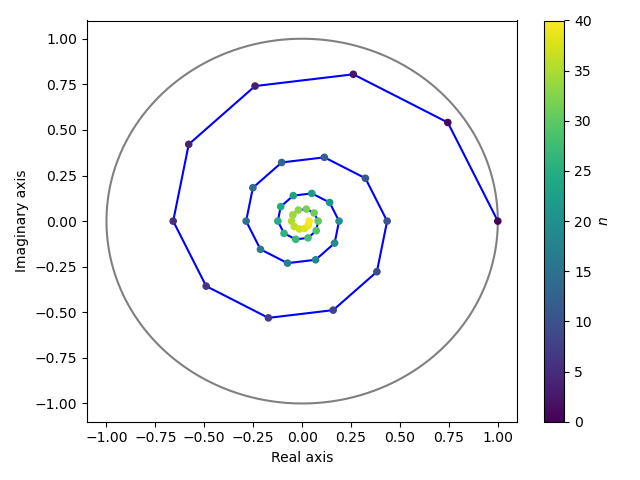
\includegraphics[width=\textwidth]{code/006_spiral/spiral.png}
\end{center}
\caption{A spiral is formed by evaluating $z^n$ with integer values of $n$ between $0$ and $41$. In this case $z = 0.92 e^{i 2\pi /20}$. The parametric curve $e^{i\theta}$ with $\theta \in \mathbb{R}$ draws a circle in the complex plane, which is depicted with a gray color. The code that generated this plot can be found in \texttt{006\_spiral/spiral.py}.}
\label{fig:spirals}
\end{figure}

\newthought{Raising a complex number to the $n$th power} can be seen as exponential scaling and rotation. Consider a complex number
\begin{equation}
  z = A e^{i\theta}
\end{equation}
where $A \in \mathbb{R}_{\ge 0}$ and $\theta \in \mathbb{R}$. If we raise this to the $n$th power, we get:
\begin{equation}
  z^n = A^n e^{i\theta n} = A^n [\cos(\theta n) + i \sin(\theta n)]\,\,.
\end{equation}
Scaling and rotation is demonstrated in Figure \ref{fig:spirals}. 

\newthought{Here are some Python examples of complex number operations}. 

\lstinputlisting[language=Python,caption={\texttt{008\_complex\_ops/ops\_example.py}},label=lst:ex1]{code/008_complex_ops/ops_example.py}





\newpage
\section{Exercises: Complex Algebra}

\begin{enumerate}
\item Prove $e^{i\pi}+1=0$ using Euler's formula. 
\item Use Euler's formula to write $1/i$ into polar form $Ae^{i\phi}$. What is the phase angle $\phi$?
\item Show that $i^{i}$ is real valued using Euler's formula. 
\item Use Euler's formula to show that de Moivre's formula is valid for $n\in\mathbb{Z}$:
$$[\cos(x)+i\sin(x)]^{n}=\cos(nx)+i\sin(nx)$$

\item Using Euler's formula, it is possible to determine the $n$th root of unity. What this means is that we look for all unique values of $z$ which satisfy the following equation where $n$ is a positive integer:
\begin{equation}
    z^{n}=1.
    \label{ch03:eq_unity}
\end{equation}
You probably already know the answer in the case of $n=2$, for which there are two solutions: $z_{0}=1$ and $z_{1}=-1$ as both $1^{2}=1$ and $(-1)^{2}=1$. \\
Provide a general formula that gives $n$ unique values of $z$ that
satisfy Equation \ref{ch03:eq_unity}. How many unique solutions of $z$ are there
for each value of $n$? Hint: remember that $e^{i 2\pi k} = 1$ where
$k$ is an integer. 
\item Use the inverse Euler formula to convert $(1-i) e^{-i \omega t} + (1+i) e^{i
  \omega t}$ into the following form:
\begin{equation*}
    A \cos(\omega t  + \phi)
\end{equation*}
with $A\in \mathbb{R}$. What is $A$ and what is $\phi$?

\item Prove using Euler's formula that:
\begin{equation*}
    \cos(3\theta )= \cos^3(\theta)-3\cos(\theta)\sin^2(\theta).
\end{equation*}

\item Use Euler's formula to prove the following trigonometric identity:
\begin{align*}
\cos(\alpha + \beta)&=\cos(\alpha)\cos(\beta) - \sin(\alpha)\sin(\beta)\,\,.
\end{align*}

\item Another definition of $e^{z}$ (the complex exponential) is by an extension of the Taylor series expansion of $e^{x}$ (the real exponential) as follows
$$e^{z}:=\sum_{k=0}^{\infty}\frac{z^{k}}{k!}, \quad\quad \text{for}\ z\in\mathbb{C}.$$
That is, $e^{z}$ is taken to mean this infinite series. Use this Taylor series expansion definition to show that
\begin{equation}
  e^{i\theta} = \cos(\theta) + i\sin(\theta).
  \label{ch03:euler_formula}
\end{equation}
To do this, compute the Taylor series expansion of $e^{i\theta}$. 

\end{enumerate}
 \ifSpExerciseSol
 \newpage
\section{Suggested solutions: Complex Algebra}
\begin{enumerate}

\item Euler's formula:
$$e^{i\theta}=\cos\theta+i\sin\theta,$$
so for $\theta=\pi$
$$e^{\pi i}=\cos(\pi)+i\sin(\pi)=-1,$$
as $\cos(\pi)=-1$ and $\sin(\pi)=0$, hence $e^{\pi i}+1=0$. 

\item Multiply by $i$ in the numerator and denominator to obtain
$$\frac{1}{i}=\frac{i}{i^{2}}=-i.$$
Using Euler's formula $e^{i\theta}=\cos\theta+i\sin\theta$ we take $\theta=\frac{3\pi}{2}$, this gives a polar representation of $-i$ as
$$-i=e^{\frac{3\pi}{2}i}.$$
\textbf{Remark}: Multiplication by $i$ rotates any vector in the complex plane by $\pi/2$ counterclockwise and $(1/i)(i)=1$, so $1/i$ rotates by $\pi/2$ clockwise, so our result makes sense. 

\item Use Euler's formula: $e^{i\theta}=\cos\theta+i\sin\theta$, with $\theta=\pi/2$. Then we can write $e^{\frac{\pi}{2}i}=i$ giving us
$$i^{i}=(e^{\frac{\pi}{2}i})^{i}=e^{\frac{\pi}{2}i^{2}}=e^{-\frac{\pi}{2}}\in\mathbb{R}.$$
Thus $i^{i}$ is a real number. 

\item Let $x$ be any real number and $n$ be an integer. Using Equation \ref{eq:complexexponentiation} we have $(e^{a})^{n}=\underbrace{e^{a}e^{a}\hdots e^{a}}_{n\ \text{times}}=e^{\overbrace{a+a+\hdots+a}^{n\ \text{times}}}=e^{an}$ therefore 
$$[\cos(x)+i\sin(x)]^{n}=(e^{ix})^{n}=e^{ixn}=\cos(nx)+i\sin(nx)$$
as desired. 

\item From the hint we have that $e^{i2\pi k}=1$ which can be combined with the fact that $(e^{a})^{n}=e^{an}$, giving that the solutions to $z^{n}=1$ are of the form
$$w_{k}=e^{\frac{2\pi i k}{n}}, \quad k=0,\hdots,n-1.$$
A simple check to see that this is what we want is that $w_{k}$ satisfy
$$(w_{k})^{n}=(e^{\frac{2\pi ik}{n}})^{n}=e^{2\pi ik}.$$
This gives $1$ since $e^{2\pi ik}=1$ for all $k\in\mathbb{Z}$. This gives $n$ unique solutions to the equation $z^{n}=1$ as expected by the Fundamental Theorem of Algebra.  

\item Referring to the previous problem.
\begin{itemize}
    \item[a)] Have that $w_{k}=e^{2\pi ik/5}$ for $k=0,1,2,3,4$. 
    \item[b-c)] See Listing \ref{exercise3.6}. The figure formed by the fifth roots of unity is a regular pentagon. 
\end{itemize}

\lstinputlisting[language=Python,caption={Solution for Exercise 3.6},label=exercise3.6]{ch03/code/ex3.6.py}

\item Have that 
\begin{align*}
    \cos(\theta)&=\frac{1}{2}(e^{i\theta}+e^{-i\theta}), \\
    \sin(\theta)&=\frac{1}{2i}(e^{i\theta}-e^{-i\theta}).
\end{align*}
Using that $1/i=-i$ from Exercise 2 we get
$$(1-i)e^{-i\omega t}+(1+i)e^{i\omega t}=(e^{i\omega t}+e^{-i\omega t})-\frac{1}{i}(e^{i\omega t}-e^{-i\omega t}).$$
By the inverse Euler relations we may write this as
$$(1-i)e^{-i\omega t}+(1+i)e^{i\omega t}=2\cos(\omega t)-2\sin(\omega t).$$
Next step is to write this as a pure cosine. That is, determine $A$ and $\phi$ such that 
$$A\cos(\omega t+\phi)=2\cos(\omega t)-2\sin(\omega t).$$
Using $\cos(\alpha+\beta)=\cos(\alpha)\cos(\beta)-\sin(\alpha)\sin(\beta)$ this can be rewritten as
$$A\cos(\omega t)\cos(\phi)-A\sin(\omega t)\sin(\phi)=2\cos(\omega t)-2\sin(\omega t).$$
Therefore $A$ and $\phi$ must satisfy
\begin{align*}
    A\cos(\phi)&=2, \\
    A\sin(\phi)&=2.
\end{align*}
In other words $A=\sqrt{2^{2}+2^{2}}=\sqrt{8}=2\sqrt{3}$ and $\tan(\phi)=1$. With $\phi$ in the first quadrant this gives $\phi=\pi/4$. Hence
$$(1-i)e^{-i\omega t}+(1+i)e^{i\omega t}=2\sqrt{3}\cos\left(\omega t+\frac{\pi}{4}\right).$$

\item Replace the cosine to obtain
$$\cos(3\theta)=\frac{1}{2}(e^{3i\theta}+e^{-3i\theta})=\frac{1}{2}((e^{i\theta})^{3}+(e^{-i\theta})^{3}).$$
When expanded the first term is
$$(\cos\theta+i\sin\theta)^{3}=\cos^{3}\theta+3i\cos^{2}\theta\sin\theta-3\cos\theta\sin^{2}\theta-i\sin^{3}\theta$$
and the second term
$$(\cos\theta-i\sin\theta)^{3}=\cos^{3}\theta-3i\cos^{2}\theta\sin\theta-3\cos\theta\sin^{2}\theta+i\sin^{3}\theta.$$
Adding these together then gives
$$\cos(3\theta)=\cos^{3}\theta-3\cos\theta\sin^{2}\theta.$$

\item Let $z_{1}=e^{\alpha i}$ and $z_{2}=e^{\beta i}$ be complex numbers. Then
$$z_{1}z_{2}=e^{\alpha i}e^{\beta i}=e^{(\alpha+\beta)i}=\cos(\alpha+\beta)+i\sin(\alpha+\beta).$$
In addition we have that
$$e^{\alpha i}e^{\beta i}=(\cos\alpha+i\sin\alpha)(\cos\beta+i\sin\beta)=(\cos\alpha\cos\beta-\sin\alpha\sin\beta)+i(\sin\alpha\cos\beta+\cos\alpha\sin\beta).$$
Taking the real and imaginary parts we get that
\begin{align*}
    \cos(\alpha+\beta)&=\cos\alpha\cos\beta-\sin\alpha\sin\beta, \\
    \sin(\alpha+\beta)&=\sin\alpha\cos\beta+\cos\alpha\sin\beta.
\end{align*}

\item Consider the complex exponential of the form $e^{i\theta}$, then by this new definition we have
$$e^{i\theta}=\sum_{k=0}^{\infty}\frac{(i\theta)^{k}}{k!}.$$
Using this definition we have
$$e^{i\theta}=\sum_{k=0}^{\infty}\frac{(i\theta)^{k}}{k!}=1+i\theta+\frac{(i\theta)^{2}}{2!}+\frac{(i\theta)^{3}}{3!}+\frac{(i\theta)^{4}}{4!}+\hdots.$$
Using that $i^{2}=-1$ we get
$$e^{i\theta}=1+i\theta-\frac{\theta^{2}}{2!}-i\frac{\theta^{3}}{3!}+\frac{\theta^{4}}{4!}+\hdots$$
Grouping terms with and without $i$ this can be written as
$$e^{i\theta}=(1-\frac{\theta^{2}}{2!}+\frac{\theta^{4}}{4!}+\hdots)+i(\theta-\frac{\theta^{3}}{3!}+\frac{\theta^{5}}{5!}-\hdots).$$
The first terms correspond to the Taylor series for $\cos \theta$ and the other $\sin \theta$. Hence we get Euler's formula
$$e^{i\theta}=\cos\theta+i\sin\theta.$$

\end{enumerate}
 \fi
\fi

\ifSpSigSys
\chapter{Signals and Systems}
% what is a signal and what is a system?
%
% introduces:
% - signal
% - continuous-time and discrete-time signal
% - dependent and independent variable
% - system
%
\newthought{What is a signal and what is a system?} By
a \emph{\index{signal}{signal}}, we mean an information carrying mathematical function. Any function that has a value as a function of one or more variables is in essence a signal. By a \emph{\index{system}{system}}, we denote a mathematical operation that modifies a signal. A system consists of the precise mathematical description of how a signal fed into a system is modified by the system to produce an output signal.

The definition of signals and systems are merely abstract concepts, which have gained acceptance in the engineering community. In the context of mathematics, signals could also be called functions or vectors. Systems would be called functions or operators. In computer science, signals are often treated as arrays of numbers in the memory of a computer and systems are algorithms and computer programs that operate on these arrays.

\section{Signals}
\index{signal}

\begin{marginfigure}%
\begin{center}
\begin{tikzpicture}
\begin{axis}[width=\textwidth,
	xticklabels=\empty,
	yticklabels=\empty,		
	xmin=-1.5,xmax=6,
	axis x line=bottom,
	axis y line=left,
	xlabel={Independent variable $t$},
	xlabel style={below},
	ylabel={Dependent variable $x(t)$},
    xlabel style={ yshift = { 1em } },
    ylabel style={ yshift = { -2.2em } }
]
\addplot[draw=blue,domain=-1:7,samples=150] {(x>0)*exp(-x)};
\end{axis}
\end{tikzpicture}
\end{center}
\caption{Continuous-time signal.}
\label{fig:ctfig}
\end{marginfigure}

\begin{marginfigure}%
\begin{center}
\begin{tikzpicture}
\begin{axis}[width=\textwidth,
%	title={Discrete-time signal},
	xticklabels=\empty,
	yticklabels=\empty,	
	xmin=-1.5,xmax=6,
	axis x line=bottom,
	axis y line=left,
	xlabel={Independent variable $n$},
	xlabel style={below},
	ylabel={Dependent variable $x[n]$},
    xlabel style={ yshift = { 1em } },
    ylabel style={ yshift = { -2.2em } }
]
\addplot+[ycomb,domain=-1:5,samples=15] {(x>0)*exp(-x)};
\end{axis}
\end{tikzpicture}
\end{center}
\caption{Discrete-time signal.}
\label{fig:dtfig}
\end{marginfigure}


\newthought{A \index{signal}{signal}} is a mathematical function $x(t)$, which describes the value of a \index{dependent variable} dependent variable $x$, as a function of an \index{independent variable}independent variable $t$. An independent variable ``sweeps'' through all possible values. The dependent variable is the variable that changes as a function of the independent variable and conveys information.

Here's an example. When describing electric potential as a function of time $V(t)$, time $t$ is the independent variable and the electric potential $V(t)$ as a function of time is the dependent variable. Time by itself does not convey information, but electric potential as a function of time does.

Physical ``real world'' signals are modeled as continuous-time signals. Examples include, amongst countless others:
\begin{itemize}
 \setlength\itemsep{0.25em}        
\item temperature,
\item density,
\item pressure as a function of time and space (sound, seismic waves),
\item electric field as a function of time and position
  (electromagnetic waves), or
\item electrical current in a circuit.
\end{itemize}
Physics relies on differential calculus, with integration and differentiation as elementary operators. As we will later see, differential calculus can be studied through methods of signal processing. Especially the spectral techniques and the Fourier transform are useful tools that can be applied in differential calculus.

This course will focus primarily on one-dimensional signals. These signals are complex valued functions $x(t) \in \mathbb{C}$ of a real valued argument $t\in \mathbb{R}$. This will naturally also cover the
special case, where the signal is real valued
$x(t) \in \mathbb{R} \subset\mathbb{C}$. 

By convention, we will refer to the independent variable of a signal as time, even though this variable doesn't necessarily have to indicate time. It can represent anything. For example, the independent variable can just as well be e.g., distance.

Signals can be continuous or discrete. Following a commonly adopted practice, we will use round brackets for continuous-time signals (e.g., $x(t)$) and square brackets for discrete-time signals (e.g., $x[n]$). 

In the case of discrete-time signals, the sample index
$n \in \mathbb{Z}$ is unitless. A discrete-time signal is merely a sequence of numbers. The only way to associate meaning to this sequence of numbers is the a priori knowledge of how the signal was discretized. This allows us to e.g., map the $n$th sample to a real valued time.

An example of a continuous-time and a discrete-time signal is shown in Figures \ref{fig:ctfig} and \ref{fig:dtfig}. When plotting signals graphically, it is customary (but not mandatory) to use the horizontal axis for the independent variable, and the dependent variable on the vertical axis.

To summarize, the two main types of signals that this course deals with are one-dimensional continuous-time $x(t)$ and one-dimensional discrete-time signals $x[n]$. Continuous-time signals are mappings from the real axis (time) to the set of complex numbers:
\begin{equation}
\boxed{
x: \mathbb{R} \rightarrow \mathbb{C}
}
\end{equation}
Discrete-time signals are mappings from the set of integers to the set of complex numbers:
\begin{equation}
\boxed{
x: \mathbb{Z} \rightarrow \mathbb{C}
}
\end{equation}
Signal processing of higher dimensional signals are essentially functions of the form
\begin{equation}
x: \mathbb{R}^N \rightarrow \mathbb{C}
\end{equation}
or in the case of discrete-time:
\begin{equation}
x: \mathbb{Z}^N \rightarrow \mathbb{C}
\end{equation}

\newthought{The first experimental detection of gravitational waves} using the Laser Inteferometer Gravitational-Wave Observatory (LIGO) is shown in Figure \ref{fig:ligo_meas}. This signal is an example of a one-dimensional signal. The signal is thought to be caused by two black holes with masses around 30 solar masses merging together, 1.3 billion light-years from Earth. The independent variable on the x-axis is time, and the dependent variable is strain (stretching) of space that occurs due to a gravitational wave passing through the instrument. This is measured by comparing the relative lengths of two 4 km long laser interferometer arms. 

\begin{figure}
\begin{center}
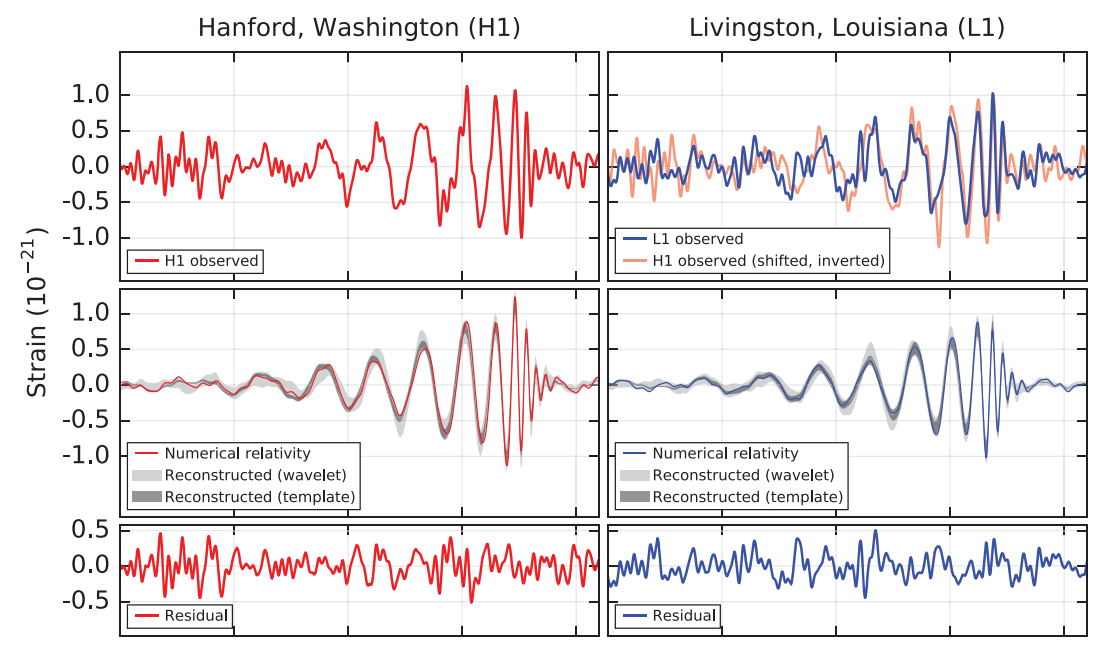
\includegraphics[width=\textwidth]{ch04/figures/dc_fg.png}
\end{center}
\caption{Two independent one dimensional signals measured by LIGO depicting strain. This is stretching of space due to a gravitational wave passing through two geographically separated laser interferometer observatories. One in Hanford, WA (left), and one in Livingston, LA (right). The figure is from: B. P. Abbott et al. (LIGO Scientific Collaboration and Virgo Collaboration) Phys. Rev. Lett. 116, 061102 – Published 11
February 2016.}
\label{fig:ligo_meas}
\end{figure}

\newthought{Signals can be of arbitrary dimension}. For example, an image is a 2d signal, where the dependent variable is intensity $I(x,y)$ measured as a function of two independent spatial variables $x$ and $y$ that indicate distance from origin along two orthogonal axes.  An example of a discrete-time two-dimensional signal is shown in Figure \ref{fig:bh_example}. It represents an image of the emission from hot gas in the event horizon of a black hole around the M87 galaxy. The image is obtained using a technique called very long baseline interferometry, which utilizes measurements from radio telescopes around the world. These measurements are combined together to simulate a large telescope with the resolution equivalent to a telescope approximately the size of Earth.\footnote{The Fourier transform, which is one of the central themes in this course, is a key part of the mathematics of very long baseline interferometric imaging.}

Even higher dimensional signals can be used. Consider for example a video. It is a signal that contains the intensity of an image as a function of time. You can think of a moving picture (movie) as a three dimensional signal: $I(x,y,t)$, where the intensity of the image is a function of two dimensional position as well as time.

While we will focus primarily on one dimensional signals in order to keep things simple, many of the concepts we discuss can be generalized to multiple dimensions. Two dimensional signal processing is called image processing, and it shares many of the same basic concepts with one dimensional signal processing. I will try to also occasionally give examples of signal processing with higher dimensional signals.

%\begin{figure}
%\begin{center}
%\includegraphics[width=\textwidth]{ch01/2dsig.png}
%\end{center}
%\label{fig:2dexim}
%\caption{An example of a 2d signal: 32-cm wavelength opposite
%  circularly polarized inverse synthetic aperture radar map of the
%  Moon, obtained using the EISCAT radar in Troms\o{}. Image intensity
%  represents backscattered power from the surface of the Moon.}
%\end{figure}

\begin{figure}
\begin{center}
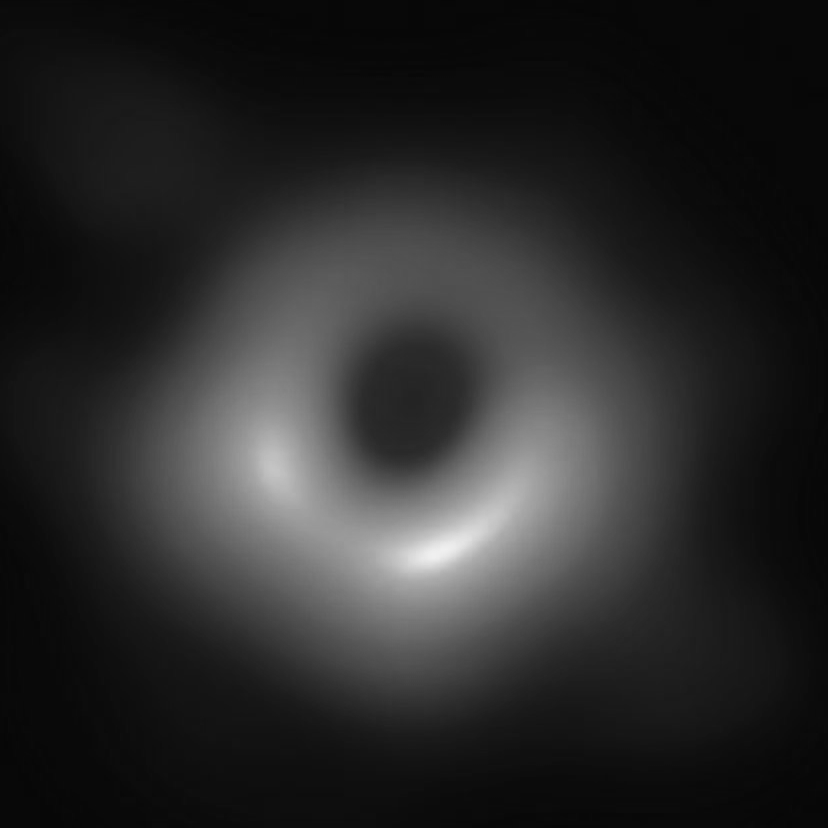
\includegraphics[width=0.68\textwidth]{ch04/figures/bhi.png}
\end{center}
\caption{An example of a 2d signal: A Very Long Baseline Interferometric radio image of
the black hole at the center of galaxy M87. The intensity depicts what is thought to be hot gas outside the event horizon of the black hole. Credit: Event Horizon Telescope collaboration et al. 2019.}
\label{fig:bh_example}
\end{figure}

\newthought{Digital signals}
in a computer are also quantized. This means that there is only a finite number of possible values for the dependent value of a signal. This type of a signal is called a \emph{\index{quantized}{quantized}} signal. We will not discuss quantization in this course.


\section{Systems}
%\newcommand{\sign}{\text{sign}}

\newthought{A signal processing \index{system}{system}} can be represented graphically as a block diagram, which describes signals going into a system, and signals going out of a system. An example is shown in
Figure \ref{simple_sps}

\begin{figure}
\tikzstyle{int}=[draw]
%\tikzstyle{init} = [pin edge={to-,thin,black}]
\tikzstyle{init} = []
% [pin edge={to-,thin,black}]

\begin{center}
  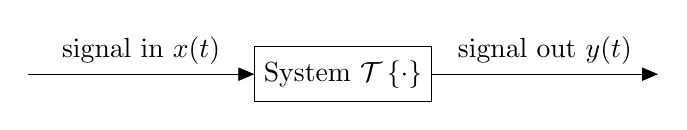
\begin{tikzpicture}[node distance=4cm,auto,line width=0.1mm,>=triangle 45]
    \node [int] (a) {System $\spop$};
    \node (b) [left of=a,node distance=4cm, coordinate] {a};
    %\node [int, pin={[init]above:$p_0$}] (c) [right of=a] {$\frac{1}{s}$};
    \node [coordinate] (end) [right of=a, node distance=4cm]{};
    \path[->] (b) edge node {signal in $x(t)$} (a);
    %\path[->] (a) edge node {$v$} (c);
    \draw[->] (a) edge node {signal out $y(t)$} (end) ;
\end{tikzpicture}
\end{center}
\label{simple_sps}
\caption{A simple signal processing system block diagram.}
\end{figure}
A graphical representation is useful for understanding a signal processing system, especially if it is a complicated one, which includes many systems and signals.

The following block diagram is a real-world example of the block diagram of the EISCAT Svalbard radar transmitter subsystem. 
\begin{figure}
\begin{center}
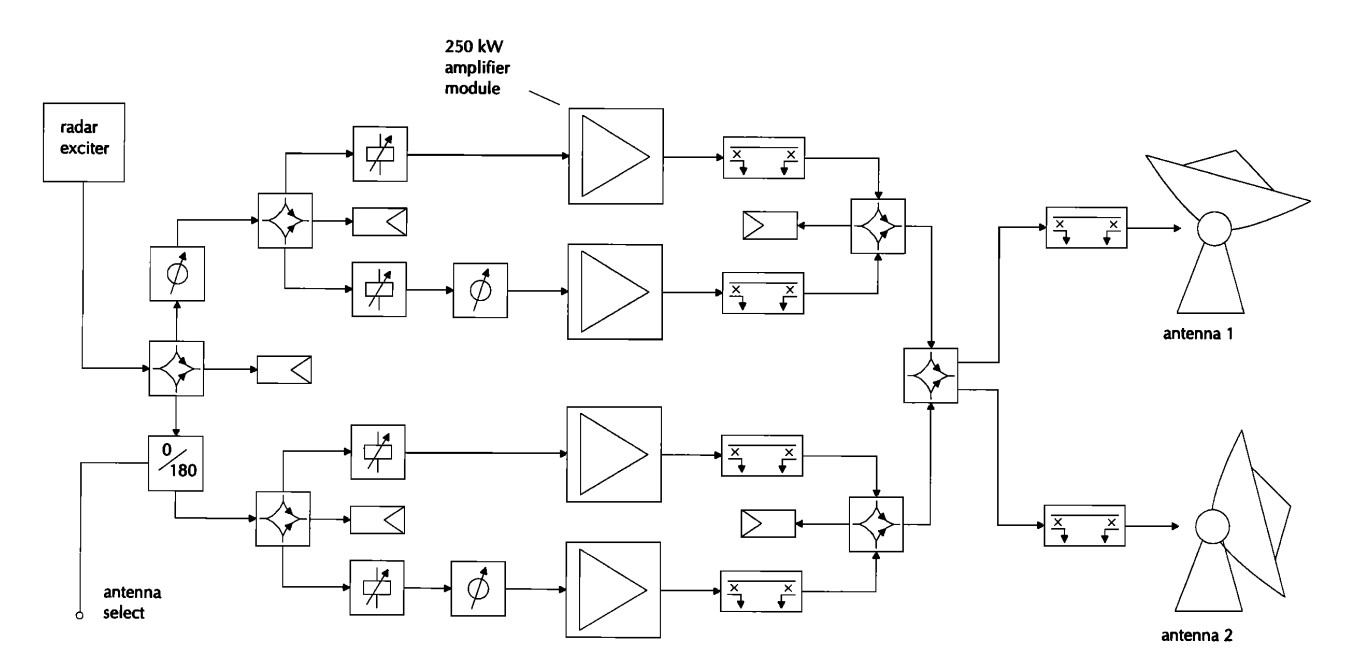
\includegraphics[width=\textwidth]{ch04/figures/wannberg97.jpg}
\end{center}
\caption{An example of a more complicated block diagram. From: Wannberg et.al., 1997.}
\label{fig:esr}
\end{figure}

The mathematical description of a system (what goes on in the box) is a general transformation of a signal. The mathematical notation for a continuous-time system in general is\footnote{Here $\spop$ is a mathematical description of how the input signal is modified by the signal processing system. This is also called an
\index{operator}{operator}}:
\begin{equation}
\boxed{
y(t) = \spop[x(t)]
}
\end{equation}
and for discrete-time system:
\begin{equation}
\boxed{
y[n] = \spopb\{x[n]\}
}
\end{equation}
An example of a system could be a function that delays the input
signal by a delay $\tau$:
\begin{equation}
y(t) = x(t-\tau).
\end{equation}
Another example is a linear amplifier, which multiplies the amplitude
of the signal with a constant $\alpha \in \mathbb{C}$:
\begin{equation}
y(t) = \alpha x(t).
\end{equation}
You will often encounter both of these types of systems.

\newthought{For example, we can use these two basic systems to make a simplified model of a radar}. Imagine that you have a radar. This radar sends out a waveform that is described by a waveform $x(t)$. Let's say that the
time it takes an electromagnetic wave to travel from the radar transmitter to a point-like radar target and back is $\tau$ seconds. The received radar echo will be a delayed version of the transmitted signal, which is delayed by $\tau$. In addition to this, the signal will be scaled, as a radar echo is typically much weaker than the transmitted signal.

Therefore, a very simple system that describes a radar echo is the following:
\begin{equation}
y(t) = \alpha x(t-\tau)
\end{equation}
where $y(t)$ is the received radar echo signal.

We can further expand this concept to write the equation that describes a radar echo for a situation where there can be a continuous radar echo at time delays between $0$ and $T$:
\begin{equation}
y(t) = \int_0^T \alpha(\tau) x(t-\tau) d\tau.
\end{equation}
In this case, $\alpha(\tau)$ describes the radar echo amplitude as a function of propagation delay. This type of an equation is called a \emph{\index{convolution}convolution} equation. You will encounter this type of equation very often in signal processing, and find that the Fourier transform is a very useful tool when dealing with convolution equations.

\newthought{Differential operators can also be seen as
systems}. Consider the first time-derivative of the continuous-time signal $x(t)$:
\begin{equation}
y(t) = \frac{d}{d t}x(t).
\end{equation}
The system definition is the time derivative operator $\frac{d}{dt}$.

\newthought{Systems are classified based on their mathematical properties}. The most important two are: \emph{\index{linearity}{linearity}} and \emph{\index{time-invariance}{time-invariance}}. A
system which is both linear and time-invariant is called 
\index{linear time-invariant}{linear time-invariant} 
(LTI)\index{LTI}. Such systems have beneficial mathematical properties that make analysis and design of such systems very straightforward. We'll later on prove that LTI systems are fully characterized by something known as an impulse response. This is an important concept in signal processing.

\section{Linear system}
\index{Linear system}

\begin{marginfigure}[-3cm]
\tikzstyle{int}=[draw, minimum size=2em]
\tikzstyle{init} = [pin edge={to-,thin,black}]

\begin{center}
% Definition of blocks:
\tikzset{%
  block/.style    = {draw, thick, rectangle, minimum height = 3em,
    minimum width = 3em},
  sum/.style      = {draw, circle, node distance = 2cm}, % Adder
  input/.style    = {coordinate}, % Input
  output/.style   = {coordinate} % Output
}
% Defining string as labels of certain blocks.
\newcommand{\suma}{\Large$+$}
\newcommand{\inte}{$\displaystyle \int$}
\newcommand{\derv}{\huge$\frac{d}{dt}$}
\newcommand{\mula}{\Large$\cross$}

\begin{tikzpicture}[auto, line width=0.1mm, node distance=2cm, >=triangle 45]
% make an op block
\draw 
   node at (0,0) [block, name=op0] {$\spop$};
% make a sum block
\draw 
   node at (-1.5,0) [sum, name=suma2] {\suma};
% output node
\draw 
   node at (1.5,0) [name=out0] {$y_1(t)$};

% input node 1
\draw 
   node at (-3,1.5) [name=in0] {$x_1(t)$};

% input node 2
\draw 
   node at (-3,-1.5) [name=in1] {$x_2(t)$};

% make a mult block
\draw 
   node at (-1.5,1.5) [sum, name=mul0] {\mula};
% make a mult block
\draw 
   node at (-1.5,-1.5) [sum, name=mul1] {\mula};

% output node
\draw 
   node at (0,1.5) [name=c0] {$c_2$};

% output node
\draw 
   node at (0,-1.5) [name=c1] {$c_1$};
% join
\draw[->](suma2) -- node {}(op0);
\draw[->](mul0) -- node {}(suma2);
\draw[->](mul1) -- node {}(suma2);
\draw[->](op0) -- node {}(out0);
\draw[->](in0) -- node {}(mul0);
\draw[->](in1) -- node {}(mul1);
\draw[->](c0) -- node {}(mul0);
\draw[->](c1) -- node {}(mul1);
\end{tikzpicture}

\vspace{1em}
\begin{tikzpicture}[auto, line width=0.1mm, node distance=2cm, >=triangle 45]
% make an op block
\draw 
   node at (-1.5,1.5) [block, name=op0] {$\spop$};
\draw 
   node at (-1.5,-1.5) [block, name=op1] {$\spop$};
% make a sum block
\draw 
   node at (0,0) [sum, name=suma2] {\suma};
% make a mult block
\draw 
   node at (0,1.5) [sum, name=mul0] {\mula};
% make a mult block
\draw 
   node at (0,-1.5) [sum, name=mul1] {\mula};
% output node
\draw 
   node at (1.5,0) [name=out0] {$y_2(t)$};
% output node
\draw 
   node at (1.5,1.5) [name=c0] {$c_2$};
% output node
\draw 
   node at (1.5,-1.5) [name=c1] {$c_1$};
% input node 1
\draw 
   node at (-3,1.5) [name=in0] {$x_1(t)$};
% input node 2
\draw 
   node at (-3,-1.5) [name=in1] {$x_2(t)$};
% join
\draw[->](suma2) -- node {}(out0);

\draw[->](in0) -- node {}(op0);
\draw[->](in1) -- node {}(op1);

\draw[->](op0) -- node {}(mul0);
\draw[->](op1) -- node {}(mul1);
\draw[->](mul0) -- node {}(suma2);
\draw[->](mul1) -- node {}(suma2);
\draw[->](c0) -- node {}(mul0);
\draw[->](c1) -- node {}(mul1);

\end{tikzpicture}
\end{center}
\label{fig:linearity_block}
\caption{In order for the system specified by $\spop$ to be linear, $y_1(t) = y_2(t)$ must be satisfied.}
\end{marginfigure}

A system is linear, if a linear combination of inputs fed into the system yields the same as the linear combination of outputs:
\begin{equation}
\boxed{
\spop[c_1 x_1(t) + c_2 x_2(t)] = c_1 \spop[x_1(t)] + c_2 \spop[ x_2(t) ]}
\label{def:linear_sys}
\end{equation}
for arbitrary constants $c_1 \in \mathbb{C}$ and $c_2 \in \mathbb{C}$ and arbitrary input signals $x_1(t)$ and $x_2(t)$. This property is highly useful, and appears throughout signal processing.

\newthought{An example of a linear system} is a system that scales the input signal by a constant factor $\alpha$:
\begin{equation}
  y(t) = \alpha x(t).
\end{equation}
If $|\alpha| >1$, the signal is amplified. This type of a system would typically be called an amplifier. If $0<|\alpha|<1$, the system would be called an attenuator, as the output signal amplitude would be attenuated.

It is quite easy to determine that the test for linearity is passed for this system:
\begin{equation}
\alpha [c_1 x_1(t) + c_2 x_2(t)] = c_1 [\alpha x_1(t)] + c_2 [\alpha x_2(t)].
\end{equation}

\newthought{An example of a non-linear system} is the following system, which obtains the absolute value of $x(t)$:
\begin{equation}
y(t) = |x(t)|
\end{equation}
It is quite clear that this does not pass the test for linearity:
\begin{equation}
|c_1 x_1(t) + c_2 x_2(t)| \ne c_1 |x_1(t)| + c_2 |x_2(t)|,
\end{equation}
for all possible values $c_1$, $c_2$, $x_1(t)$, and $x_2(t)$.
\begin{marginfigure}
\tikzstyle{int}=[draw, minimum size=2em]
\tikzstyle{init} = [pin edge={to-,thin,black}]

\begin{center}

% Definition of blocks:
\tikzset{%
  block/.style    = {draw, thick, rectangle, minimum height = 3em,
    minimum width = 3em},
  sum/.style      = {draw, circle, node distance = 2cm}, % Adder
  input/.style    = {coordinate}, % Input
  output/.style   = {coordinate} % Output
}
% Defining string as labels of certain blocks.
\newcommand{\suma}{\Large$+$}
\newcommand{\inte}{$\displaystyle \int$}
\newcommand{\derv}{\huge$\frac{d}{dt}$}
\newcommand{\mula}{\Large$\cross$}

\begin{tikzpicture}[auto, line width=0.1mm, node distance=2cm, >=triangle 45]
% make an op block
\draw  
node at (-1.0,3.0) [name=in0] {$x(t)$};

% make an op block
\draw  
node at (-1.0,1.5) [block, name=op0] {$\spop$};

\draw  
node at (-1.0,0) [block, name=delay0] {Delay};

% output node
\draw 
 node at (-1.0,-1.5) [name=out0] {$y_2(t)$};

% make an op block
\draw  
node at (1.0,3.0) [name=in1] {$x(t)$};

% make an op block
\draw  
node at (1.0,0.0) [block, name=op1] {$\spop$};

\draw  
node at (1.0,1.5) [block, name=delay1] {Delay};

% output node
\draw 
 node at (1.0,-1.5) [name=out1] {$y_1(t)$};

% join
\draw[->](in0) -- node {}(op0);
\draw[->](op0) -- node {}(delay0);
\draw[->](delay0) -- node {}(out0);


% join
\draw[->](in1) -- node {}(delay1);
\draw[->](delay1) -- node {}(op1);
\draw[->](op1) -- node {}(out1);


\end{tikzpicture}
\end{center}
\caption{In order for the system specified by $\spop$ to be time-invariant, $y_1(t) = y_2(t)$ must be satisfied. \label{fig:time_inv_block}}
\end{marginfigure}

\section{Time-invariant system}
\index{Time-invariant}

Let us first define a delay system $\mathcal{D}\{x(t)\} = x(t-\tau)$. Let us assume that the output of a system is $y(t) = \spop[x(t)]$. This system is time-invariant if:
\begin{equation}
\boxed{
\mathcal{T}\{\mathcal{D}\{x(t)\}\} = \mathcal{D}\{\mathcal{T}\{x(t)\}\}
\label{def:timeinv}
}
\end{equation}
In other words, it does not matter if the signal is delayed before or after the system $\mathcal{T}\{\cdot\}$. To check time-invariance we need to verify Equation \ref{def:timeinv}. 

The test for time-invariance is illustrated as a block diagram in Figure \ref{fig:time_inv_block}. If you want, you could think of a time-invariant system as a system that satisfy
$$[\mathcal{T},\mathcal{D}]x(t)=0,$$
where $[\mathcal{T},\mathcal{D}]=\mathcal{T}\mathcal{D}-\mathcal{D}\mathcal{T}$ is the commutator of two operators. Thus, a time-invariant system $\mathcal{T}$ is a system that commutes with the time-delay operator $[\mathcal{T},\mathcal{D}]=0$. 

\newthought{An example of a time-invariant system} is the system that returns the absolute value of the input signal $y(t)=|x(t)|$. We can see this by evaluating:
\begin{align}
\mathcal{T}\{\mathcal{D}\{x(t)\}\} &= \mathcal{T}\{x(t-\tau)\}=|x(t-\tau)|\\
\mathcal{D}\{\mathcal{T}\{x(t)\}\} &= \mathcal{D}\{|x(t)|\}=|x(t-\tau)|
\end{align}
Time-invariance holds as the outputs are equal. It doesn't matter if a time-delay is applied to the signal before or after obtaining the absolute value of the input signal.

\newthought{An example of a case that is not time-invariant} is $y(t) = \mathcal{T}\{x(t)\} = t + x(t)$. We can immediately see that the system directly depends on $t$, not only through the input. The formal test also shows that time-invariance is not met:
\begin{align}
\mathcal{T}\{\mathcal{D}\{x(t)\}\} &= \mathcal{T}\{x(t-\tau)\}=t+x(t-\tau) \\
\mathcal{D}\{\mathcal{T}\{x(t)\}\} &= \mathcal{D}\{t + x(t)\}=(t-\tau)+x(t-\tau)
\end{align}
In this case $\mathcal{T}\{\mathcal{D}\{x(t)\}\}\neq\mathcal{D}\{\mathcal{T}\{x(t)\}\}$ so the system is not time-invariant.

\section{Example: Overdriven amplifier}
\begin{marginfigure}
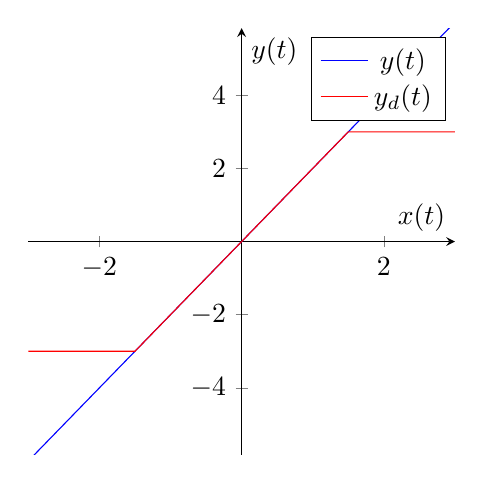
\begin{tikzpicture}
	\begin{axis}[
		xmin=-3, xmax=3,
		height=7cm,
		width=7cm,
		axis x line=center,
		axis y line=center,
                ylabel=$y(t)$,
		xlabel=$x(t)$
	]
		
	\addplot[mark=none,color=blue] {2*x};
	\addlegendentry{$y(t)$}

	\addplot[mark=none,color=red] coordinates {
		(-100,-3)
		(-1.5,-3)
		(1.5,3)
		(100,3)
	};
	\addlegendentry{$y_d(t)$}
	\end{axis}
\end{tikzpicture}
\caption{The system function of a linear amplifier $y(t)$ and a clipping amplifier system $y_d(t)$.}
\label{dist_effect}
\end{marginfigure}

A simple model of a distorted guitar amplifier system would be the
following clipping amplifier system, which is specified as follows:
\begin{equation}
y_d(t) = \left\{
  \begin{array}{rcr}
    -\beta & \mathrm{when} & \alpha x(t)<-\beta \\
    \alpha x(t) & \mathrm{when} & |\alpha x(t)| \le \beta \\
    \beta & \mathrm{when} & \alpha x(t)>\beta 
\end{array}
\right.
\label{clipamp}
\end{equation}
This is a very approximative model of an overdriven guitar
amplifier. This type of a system is often encountered in guitar music from the 50s and onwards. I'm sure that once you later implement this in practice, you'll recognize the sound that this system makes.

What does this system do? It amplifies the signal, but only up to a certain point. Beyond a certain absolute value of the input, the output maintains a constant positive or negative value.  This type of a behavior is also sometimes called clipping, and the effect is
also sometimes called distortion, as the input signal amplitude is not linearly scaled, but it is rather distorted.

\begin{marginfigure}
  \begin{center}
    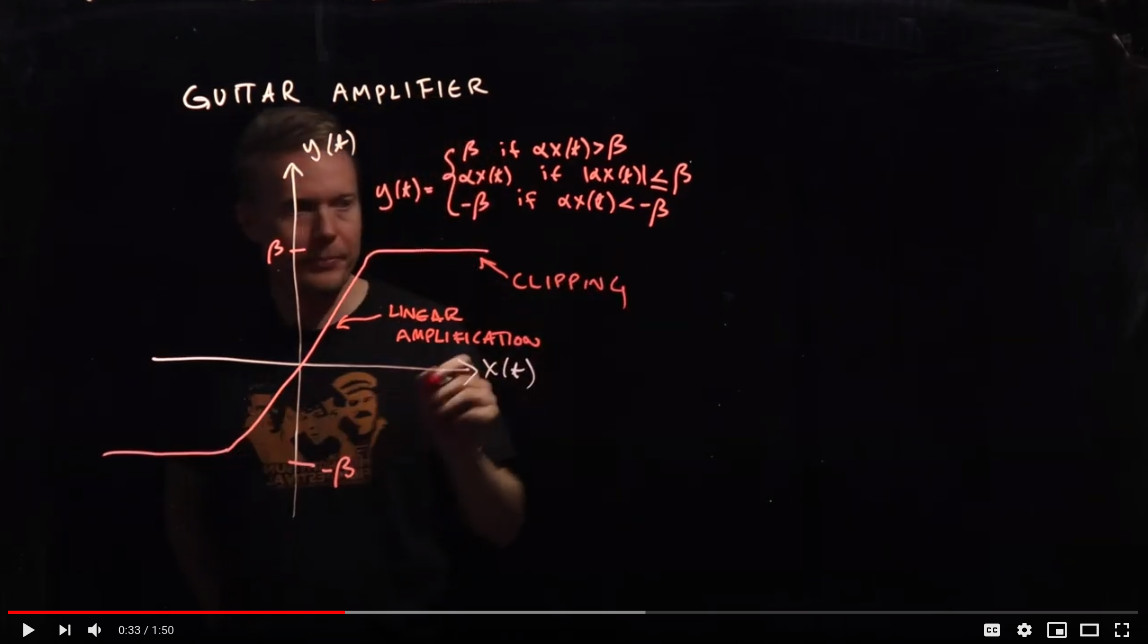
\includegraphics[width=\textwidth]{ch04/figures/ampvid.jpg}
  \end{center}
  \caption{A video discussing an overdriven guitar amplifier can be found here: \url{https://youtu.be/I30Mn_-yYF8}.}
\end{marginfigure}
Many real world amplifier systems have this type saturation behaviour. What this often means in practice is that the system is linear when the input absolute amplitude is less than some critical value, but beyond this, linearity no longer holds.

Figure \ref{dist_effect} illustrates what $y_d(t)$ would look like as a function of $x(t)$. It is compared with a normal amplifier system $y(t)=\alpha x(t)$, which does not clip.

\if 0
\begin{center}
\includegraphics[width=0.68\textwidth]{ch01_guitar_amp/clipamp.png}
\end{center}
\fi

\newpage
\section{Exercises: Signals and Systems}
\begin{enumerate}

\item Consider the following signal $V(t)$, which describes the electric potential of a circuit as a function of time. The instantaneous power flowing through this circuit is given by the following equation:
\begin{equation*}
    P(t)=R^{-1}[V(t)]^2.
\end{equation*}
It is possible to consider the function $R^{-1}[\cdot]^2$ that converts electric potential into power as a system in signal processing terminology.
\begin{enumerate}[a)]
\item Is this system linear?
\item Is this system time invariant?
\end{enumerate}
Prove your result.

\item A discrete-time system is defined as:
\begin{equation}
  y[n]= \frac{1}{5}\sum_{k=0}^{4} x[n-k].
\end{equation}
  \begin{enumerate}[a)]
  \item Explain in words what this system does to the input signal $x[n]$.
  \item Is this system linear?
  \item Is this system time-invariant?
  \end{enumerate}
Use the tests for linearity and time-invariance to justify your result. 

\item A time scaling system adjusts the scaling of the independent variable: $y(t) = x(\alpha t)$,
when $x(t)$ is the signal fed into the system and $y(t)$ is the output.

\begin{enumerate}[a)]
\item What is the effect on the signal when $0<\alpha<1$?
\item What about $\alpha>1$?
\item Is this system linear?
\item time-invariant?
\end{enumerate}

\item Prove that the time derivative operator $y(t) = \mathcal{T}\{x(t)\} = \frac{d}{dt} x(t)$
is a linear time-invariant system.

\item The guitar amplifier system given in Equation \ref{clipamp} is not a linear system. Prove this. Hint: you can use proof by example, by finding a case where the requirement of linearity is not met. 

\item Is the guitar amplifier system given in Equation \ref{clipamp} a time-invariant system? Prove your result by using the formal test for time-invariance.

\item The code in Listing \ref{lst:audio} implements a linear amplifier system for an audio signal:
\begin{equation}
y(t) = \alpha x(t)
\end{equation}
where the input signal is $x(t)$, the output signal is $y(t)$, and the amplification is $\alpha$. You can find the code and audio file on Github.
\lstinputlisting[language=Python,caption={\texttt{003\_guitar/amplifier.py}},label=lst:audio]{ch04/code/amplifier.py}
Run this code and verify that the audio signal stored in
file \verb|guitar_amp.wav| is amplified. You will need to do this by inspecting a before and after amplification plot of the audio signal, as the example code will normalize the amplitude of the signal before storing it to file.

You can use this script as a basis for experimenting with audio signal processing later on during this course.

\item Change the code in Listing \ref{lst:audio} is such a way that it implements a clipping amplifier as shown in Equation: \ref{clipamp}. Figure out suitable values for $\alpha$ and $\beta$ that make the guitar sound distorted.

\end{enumerate}

 \ifSpExerciseSol
 \newpage
\section{Suggested solutions: Signals and Systems}
\begin{enumerate}
\item

\begin{enumerate}[a)]
\item To check linearity of a system, we check Equation \ref{def:linear_sys}:
\begin{align*}
    \mathcal{T}\{c_{1}x_{1}(t)+c_{2}x_{2}(t)\}&=R^{-1}[c_{1}x_{1}(t)+c_{2}x_{2}(t)], \\
    c_{1}\mathcal{T}\{x_{1}(t)\}+c_{2}\mathcal{T}\{x_{2}(t)\} &=c_{1}R^{-1}[V_{1}(t)]^{2} + c_{2}R^{-1}[V_{2}(t)]^{2},
\end{align*}
these are not equal, so the system is not a linear system. 

\item To check time-invariance for this system, verify Equation \ref{def:timeinv}:
\begin{align*}
    \mathcal{T}\{\mathcal{D}(V(t))\}&=\mathcal{T}\{V(t-\tau)\}=R^{-1}[V(t-\tau)]^{2}, \\
    \mathcal{D}\{\mathcal{T}\{V(t)\}\}&=\mathcal{D}\{R^{-1}[V(t)]^{2}\}=R^{-1}[V(t-\tau)]^{2}.
\end{align*}
Here we get that the outputs are equal, hence the system is time-invariant. 
\end{enumerate}

\item
Consider the discrete-time system defined as:
$$y[n]=\frac{1}{5}\sum_{k=0}^{4}x[n-k].$$

\item[a)]
This system averages the past four values of $x[n]$, including $x[n]$ itself. 

\item[b)] Have that:
\begin{align*}
    \mathcal{T}\{c_{1}x_{1}[n]+c_{2}x_{2}[n]\} &= \frac{1}{5}\sum_{m=0}^{4}[c_{1}x_{1}[n-m]+c_{2}x_{2}[n-m]], \\
    c_{1}\mathcal{T}\{x_{1}[n]\}+c_{2}\mathcal{T}\{x_{2}[n]\}&=c_{1}\frac{1}{5}\sum_{j=0}^{4}x_{1}[n-j]+c_{2}\frac{1}{5}\sum_{k=0}^{4}x_{2}[n-k]
    =\frac{1}{5}\sum_{m=0}^{4}[c_{1}x_{1}[n-m]+c_{2}x_{2}[n-m]].
\end{align*}
In the last step the two sums were combined into one and the index was renamed to $k$. 
From this we can see that the output are equal, so the system is linear. 

\item[c)] To check time-invariance we calculate:
\begin{align*}
    \mathcal{T}\{\mathcal{D}\{x[n]\}\}&=\mathcal{T}\{x[n-\tau]\}=\frac{1}{5}\sum_{k=0}^{4}x[(n-\tau)-k], \\
    \mathcal{D}\{\mathcal{T}\{x[n]\}\}&=\mathcal{D}\left\{\frac{1}{5}\sum_{k=0}^{4}x[n-k]\right\}=\frac{1}{5}\sum_{k=0}^{4}x[(n-k)-\tau].
\end{align*}
These are equal upon rearranging the parenthesis, hence $\mathcal{T}\{\cdot\}$ is time-invariant. 

\item Consider a time-scaling system of the form $y(t)=x(\alpha t)$, where $x(t)$ is the input signal to the system. 

\begin{enumerate}[a)]
\item If $0<\alpha<1$, the output signal gets stretched, becoming wider. In effect, it reduces the frequency of the original signal. 
To see this compare $\sin(t)$ with $\sin(0.5t)$ as an example. 

\item If $\alpha>1$, the original frequencies are increased by a factor of $\alpha$, giving more oscillations in the signal. 
Again, compare $\sin(t)$ with $\sin(2t)$ as an example.

\item Let's check if the system is linear. Have that:
\begin{align*}
    \mathcal{T}\{c_{1}x_{1}(t)+c_{2}x_{2}(t)\}&= c_{1}x_{1}(\alpha t) + c_{2}x_{2}(\alpha t), \\
    c_{1}\mathcal{T}\{x_{1}(t)\}+c_{2}\mathcal{T}\{x_{2}(t)\}&=c_{1}x_{1}(\alpha t)+c_{2}x_{2}(\alpha t),
\end{align*}
so the system is linear as these are equal.

\item Checking time-invariance:
\begin{align*}
    \mathcal{T}\{\mathcal{D}\{x(t)\}\}&=\mathcal{T}\{x(t-\tau)\}=x(\alpha(t-\tau)), \\
    \mathcal{D}\{\mathcal{T}\{x(t)\}\}&=\mathcal{D}\{x(\alpha t)\}=x(\alpha(t-\tau)).
\end{align*}
The system is time-invariant as these satisfy Equation \ref{def:timeinv}.
\end{enumerate}

\item Consider the derivative as a system $\mathcal{T}\{x(t)\}=\frac{d}{dt}x(t)$. 
This system is time-invariant and linear. It is linear since:
\begin{align*}
    \mathcal{T}\{c_{1}x_{1}(t)+c_{2}x_{2}(t)\}&=c_{1}\frac{d}{dt}x_{1}(t) + c_{2}\frac{d}{dt}x_{2}(t), \\
    c_{1}\mathcal{T}\{x_{1}(t)\}+c_{2}\mathcal{T}\{x_{2}(t)\}&=c_{1}\frac{d}{dt}x_{1}(t) + c_{2}\frac{d}{dt}x_{2}(t),
\end{align*}
are equal, which follows from the linearity of the differential operator.

For time-invariance, we check the condition in Equation \ref{def:timeinv}:
\begin{align*}
    \mathcal{T}\{\mathcal{D}\{x(t)\}\}&=\mathcal{T}\{x(t-\tau)\}=\frac{d}{dt}x(t-\tau), \\
    \mathcal{D}\{\mathcal{T}\{x(t)\}\}&=\mathcal{D}\left\{\frac{d}{dt}x(t)\right\}=\frac{d}{dt}x(t-\tau).
\end{align*}
Showing that Equation \ref{def:timeinv} holds, hence the system is time-invariant. 

\item The guitar amplifier is a system of the form:
$$y(t)=\begin{cases}
    -\beta, \quad \hspace{0.4cm} \alpha x(t)<-\beta,  \\
    \alpha x(t), \quad |\alpha x(t)|\le \beta, \\
    \beta, \quad \hspace{0.7cm}\alpha x(t)>\beta.
\end{cases}$$
The system is not linear. To show this, find a counter example. The linearity should hold for all signals $x(t)$. 
In particular, consider two signals for which $\alpha x_{1}(t)=\beta$ and $\alpha x_{2}=\beta$. 
For these signals we get:
$$\mathcal{T}\{\alpha x_{1}(t)\}+\mathcal{T}\{\alpha x_{2}(t)\}=\beta+\beta=2\beta,$$
while:
$$\mathcal{T}\{\alpha x_{1}(t)+\alpha x_{2}(t)\}=\mathcal{T}\{\beta+\beta\}=\mathcal{T}\{2\beta\}=\beta,$$
as $2\beta > \beta$ by the last condition, hence we get $\mathcal{T}\{2\beta\}=\beta$. 
Thus, we get a contradiction in that $2\beta=\beta$ for all $\beta$, hence the system is non-linear. 

\item For the guitar amplifier of the form:
\begin{equation*}
y_d(t) = \left\{
  \begin{array}{rcr}
    -\beta & \mathrm{when} & \alpha x(t)<-\beta, \\
    \alpha x(t) & \mathrm{when} & |\alpha x(t)| \le \beta, \\
    \beta & \mathrm{when} & \alpha x(t)>\beta.
\end{array}
\right.
\end{equation*}
Have that:
\begin{align*}
    \mathcal{T}\{\mathcal{D}\{x(t)\}\}&=\mathcal{T}\{x(t-\tau)\}=\begin{cases}
        -\beta, \quad \text{for}\ \alpha x(t-\tau)<-\beta,\\
        \alpha x(t-\tau), \quad \text{for}\ |\alpha x(t-\tau)|\le \beta,\\
        \beta, \quad \text{for}\ \alpha x(t-\tau)>\beta.
    \end{cases} \\
    \mathcal{D}\{\mathcal{T}\{x(t)\}\}&=\mathcal{D}\left\{\begin{cases}
        -\beta, \quad \text{for}\ \alpha x(t)<-\beta,\\
        \alpha x(t), \quad \text{for}\ |\alpha x(t)|\le \beta,\\
        \beta, \quad \text{for}\ \alpha x(t)>\beta.
    \end{cases}\right\}=\begin{cases}
        -\beta, \quad \text{for}\ \alpha x(t-\tau)<-\beta,\\
        \alpha x(t-\tau), \quad \text{for}\ |\alpha x(t-\tau)|\le \beta,\\
        \beta, \quad \text{for}\ \alpha x(t-\tau)>\beta,
    \end{cases} \\ 
\end{align*}
so the system is time-invariant. 

\item Running Listing \ref{lst:audio} and looking at the resulting plot, one can see that the signal has been amplified. 
\lstinputlisting[language=Python,caption={Solution for Exercise 4.7},label=ex4.7,linerange={0-44}]{ch04/code/ex4.7.py}
The output from this system is shown below. 
\begin{figure}
\centering
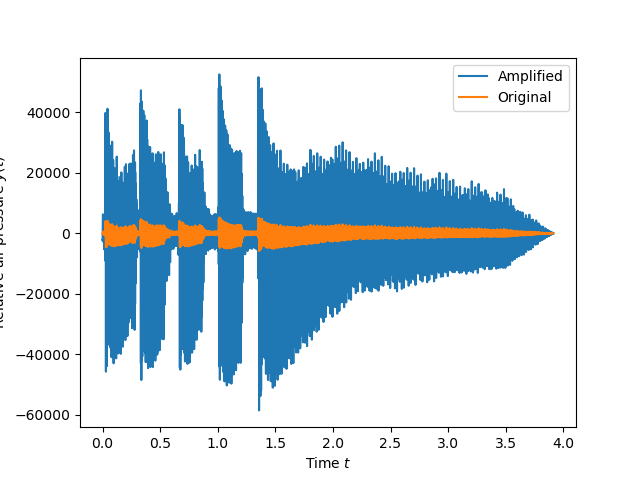
\includegraphics[scale=0.9]{ch04/figures/ex7_plot.png}
\end{figure}

\item Running Listing \ref{ex4.8} applies a distortion effect to the signal. 
\lstinputlisting[language=Python,caption={Solution for Exercise 4.8},label=ex4.8,linerange={0-47}]{ch04/code/ex4.8.py}

\end{enumerate}
 \fi
\fi

\ifSpElSig
\chapter{Elementary Signals}
%
% Continuous-time signals
% Commonly encountered special functions
% 
% - Dirac delta
% - Unit-step function
% - 
%
\newthought{There are two important elementary signals} which you will encounter throughout signal processing: the \emph{\index{unit impulse}{unit impulse}} $\delta(t)$ and the \emph{\index{unit step}{unit step}} function $u(t)$. Both of these functions have continuous-time and discrete-time counterparts.

\newthought{The unit impulse function $\delta(t)$} is a special distribution function\footnote{The unit impulse function is also known as the \emph{\index{Dirac delta function}{Dirac delta function}}, after physicist Paul Dirac, who used this function for modeling the distribution of electrical point-charges (e.g., electrons and protons)}, which is infinitely narrow, non-zero valued only at $t=0$. And when you integrate over this function, the result will be 1.

It is possible to define $\delta(t)$ in several different ways as a limit of functions with a well defined area and width $\sigma$. I'll use the Gaussian density function:
\begin{equation}
\delta_\sigma(t) = \frac{1}{\sqrt{2\pi \sigma^2}}e^{-\frac{t^2}{2\sigma^2}}\,\,.
\end{equation}
The Gaussian density function is shown in Figure \ref{fig:gauss_dens} for two different standard deviations $\sigma_1$ and $\sigma_2$. The smaller the value of $\sigma$, the more narrow the function is.

\begin{marginfigure}
\begin{center}
        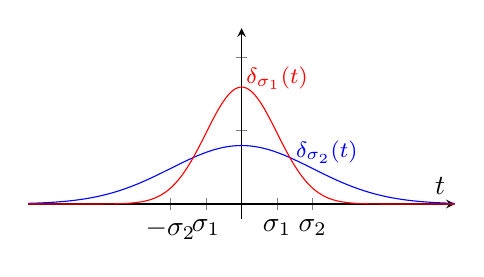
\begin{tikzpicture} \begin{axis}[width=7cm,height=4cm,ymin=-0.1,xmin=-3,ymax=1.2,xmax=3,
        yticklabels={,,}, xtick={-1,-0.5,0,0.5,1},
        xticklabels={$-\sigma_2$,$\sigma_1$,0,$\sigma_1$,$\sigma_2$},
        xlabel=$t$, axis lines = center]

%\addplot +[dirac] coordinates {(1,1.4)};
%\node at (axis cs:1.2,0.85) [below, font={\footnotesize}]{$\delta(t-t_0)$};

\node at (axis cs:1.2,0.5) [below, font={\footnotesize},color=blue]{$\delta_{\sigma_2}(t)$};
\addplot[samples=400,mark=none,color=blue]{(1/sqrt(2*3.14))*exp(-x^2/2.0)};

\node at (axis cs:0.5,1.0) [below, font={\footnotesize},color=red]{$\delta_{\sigma_1}(t)$};
\addplot[samples=400,mark=none,color=red]{(1/sqrt(2*3.14*0.25))*exp(-x^2/(2.0*0.25))};

  
\end{axis}
\end{tikzpicture}
\end{center}
\caption{A Gaussian density function becomes a unit impulse $\delta(t)$
when the width parameter approaches zero $\sigma \rightarrow 0$.}
\label{fig:gauss_dens}
\end{marginfigure}
\pgfplotsset{
    dirac/.style={
        mark=triangle*,
        mark options={scale=2},
        ycomb,
        scatter,
        visualization depends on={y/abs(y)-1 \as \sign},
        scatter/@pre marker code/.code={\scope[rotate=90*\sign,yshift=-2pt]}
    }
}
\begin{marginfigure}[0cm]
\begin{center}
        \begin{tikzpicture}
        \begin{axis}[width=7cm,height=4cm,ymin=0,xmin=-0.5,ymax=1.1,xmax=1.5,         
        yticklabels={,,},
        xtick={1},
        xticklabels={$\tau$},
        xlabel=$t$, axis lines = center]

\addplot +[dirac] coordinates {(1,1)};
\node at (axis cs:0.68,1) [below, font={\footnotesize}]{$\delta(t-\tau)$};

\end{axis}
\end{tikzpicture}
\end{center}

\caption{A unit impulse is typically depicted with a vertical arrow. A unit impulse $\delta(t-\tau)$ is centered at $t=\tau$. This is the only value of $t$ where the unit impulse is non-zero.}
\label{fig:uparrow}
\end{marginfigure}

As a result of how the function is defined, an integral over
$\delta_{\sigma}(t)$ is always unity. This is perhaps not a surprise
as this function is used in statistics as a probability density
function:
\begin{equation}
\int_{-\infty}^{\infty}\delta_\sigma(t)dt = 1 \,\,.
\end{equation}
The Dirac delta function $\delta(t)$ can be thought of as the limit when the standard deviation of this distribution approaches zero:
\begin{equation}
\lim_{\sigma\rightarrow 0}  \int_{-\infty}^{\infty} \delta_\sigma(t) dt = \int_{-\infty}^{\infty} \delta(t) dt = 1
\end{equation}
It is hopefully not difficult to convince yourself that the integral
evaluates to unity even as $\sigma \rightarrow 0$. But what does the
function $\delta(t)$ look like? First of all, it is infinitely narrow, with only one non-zero value at zero:
\begin{equation}
\delta(t) = \left\{ \begin{array}{ccc}
\infty & \mathrm{when} & t=0\\
0 &  \mathrm{when} & t \ne 0
\end{array}\right.
\end{equation}
When plotting this function, it is customary to utilize an up arrow, as shown in Figure \ref{fig:uparrow}. The figure also demonstrates how it is possible to shift the location of the peak by subtracting a constant $\tau$ from the argument of the function.

\begin{marginfigure}[0cm]
\begin{center}
        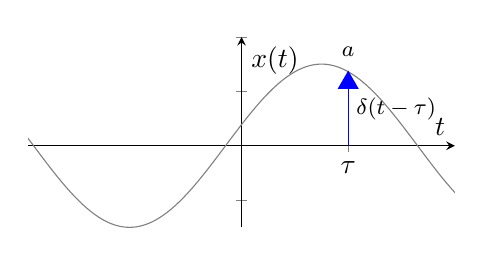
\begin{tikzpicture}
          \begin{axis}[width=7cm,height=4cm,ymin=-1.5,xmin=-2,ymax=2,xmax=2,         yticklabels={,,},
              xtick={1.0},
                      xticklabels={$\tau$},
%        xticklabels={,,},
        ylabel=$x(t)$,
    xlabel=$t$, axis lines = center]

\addplot +[dirac] coordinates {(1,1.36)};
\node at (axis cs:1.45,1.05) [below, font={\footnotesize}]{$\delta(t-\tau)$};
%\node at (axis cs:0.5,1.8) [below, font={\footnotesize}]{$x(t)$};

\node at (axis cs:1.0,2.0) [below, font={\footnotesize}]{$a$};

%\addplot[samples=400,mark=none,color=gray]{0.1*x*x*x-0.7*x*x + x + 1};
\addplot[samples=400,mark=none,color=gray]{1.5*sin(100*x+15)};
  
\end{axis}
        \end{tikzpicture}
\end{center}
\caption{The unit impulse ``selects'' the value of a continuous-time signal $x(\tau)=a$.}
\end{marginfigure}

\begin{marginfigure}
\begin{center}
        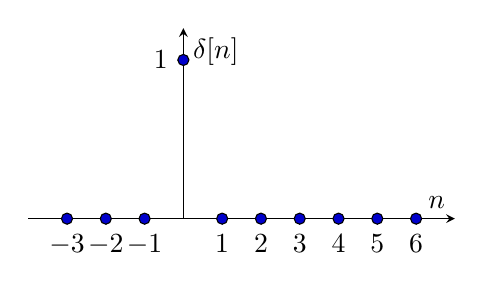
\begin{tikzpicture}
        \begin{axis}[width=7cm,height=4cm,ymin=0,xmin=-4,ymax=1.2,xmax=7,
        xtick={-3,-2,-1,0,1,2,3,4,5,6},
        ytick={0,1,2,3},
        ylabel={$\delta[n]$},
    xlabel={$n$}, axis lines = center]
   \addplot+[ycomb,color=black] plot coordinates {(-3,0) (-2,0) (-1,0) (0,1) (1,0) (2,0) (3,0) (4,0) (5,0) (6,0)};
\end{axis}
        \end{tikzpicture}
\end{center}
\caption{The discrete-time unit impulse.}
\label{fig:udensdisc}
\end{marginfigure}

The main application of the unit impulse function in signal processing is selecting or ``sampling'' a value of a signal. This is also sometimes referred to as the \emph{\index{sifting}{sifting}} property. Consider a function $x(t)$ which has the value $x(\tau) = a$. If we integrate over the function $x(t)\delta(t-\tau)$, we obtain:
\begin{equation}
\int_{-\infty}^{\infty}x(t)\delta(t-\tau) dt = x(\tau) = a\,\,.
\end{equation}
This type of integral will often appear when relating a continuous-time theory to a discrete-time theory. If you are still having a difficult time convincing yourself why the integral above results in the value it does, try thinking about it through the limit:
\begin{equation}
\lim_{\sigma\rightarrow 0}\int_{-\infty}^{\infty}x(t)\delta_{\sigma}(t-\tau) dt = x(\tau) = a\,\,.
\end{equation}
The Dirac delta function is only used in this course inside an integral, so that dealing with a singularity ($\infty$) is avoided.

\if 0
\begin{equation}
    \lim_{\sigma \rightarrow 0} \delta_{\sigma}(t) = \delta(t)\,\,,
\end{equation}
where the uniform density function $\delta_{\sigma}(t)$ is defined as:
\begin{equation}
\delta_{\sigma}(t) =\left\{ \begin{array}{cl}
\sigma^{-1}, & -\frac{1}{2}\sigma < t < \frac{1}{2}\sigma \\
0, & \mathrm{otherwise}. \end{array}
\right.\,\,.
\end{equation}
This function is identical to the probability density function of a
uniformly distributed random variable. The function
$\delta_{\sigma}(t)$ is depicted for two different values of $\sigma$
in Figure \ref{fig:udens}. It is a rectangle with width $\sigma$ on
the t-axis and an amplitude of $1/\sigma$:
\begin{marginfigure}
\begin{center}
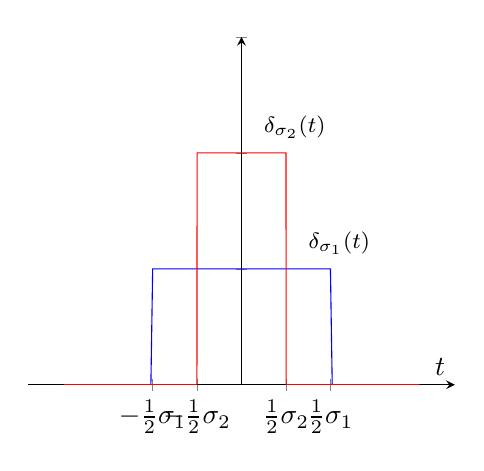
\begin{tikzpicture}
        \begin{axis}[width=7cm,height=6cm,ymin=0,xmin=-1.2,ymax=3.0,xmax=1.2,         yticklabels={,,},
        xtick={-0.5,-0.25,0.25,0.5},
        xticklabels={$-\frac{1}{2}\sigma_1$,$-\frac{1}{2}\sigma_2$,$\frac{1}{2}\sigma_2$,$\frac{1}{2}\sigma_1$},
    xlabel=$t$, axis lines = center]
\addplot[color=blue] plot coordinates {(-1,0) (-0.51,0.0) (-0.5,1.0)(0.5,1.0) (0.51,0.0) (1,0)};
\addplot[color=red] plot coordinates {(-1,0) (-0.251,0.0) (-0.25,2.0)(0.25,2.0) (0.251,0.0) (1,0)};

\node at (axis cs:0.55,1.4) [below, font={\footnotesize}]{$\delta_{\sigma_1}(t)$};

\node at (axis cs:0.3,2.4) [below, font={\footnotesize}]{$\delta_{\sigma_2}(t)$};
\end{axis}
\end{tikzpicture}
\end{center}
\caption{A rectangular pulse signal becomes a unit impulse when the width parameter $\sigma_1 \rightarrow 0$ approaches zero.}
\label{fig:udens}
\end{marginfigure}
\fi

%\newthought{The unit impulse can also be defined as an infinitely narrow Gaussian density function}:

\newthought{The discrete-time unit impulse $\delta[n]$} is defined as:
\begin{equation}
\delta[n] = \left\{\begin{array}{cl}
1 &~~~ n = 0 \\
0 &~~~ n \ne 0 \\
\end{array}
\right.\,\,.
\end{equation}
The discrete-time unit impulse signal is shown in
Figure \ref{fig:udensdisc}. In most cases, the discrete-time unit
impulse serves a similar function as its continuous-time equivalent.

%\newpage
%\subsection{Unit step}

\tikzstyle{int}=[draw, minimum size=2em]
\tikzstyle{init} = [pin edge={to-,thin,black}]
\begin{marginfigure}[-3cm]
\begin{center}

        \begin{tikzpicture}
        \begin{axis}[width=7cm,height=4cm,ymin=0,xmin=-2,ymax=1.3,xmax=2, 
                ytick={0,1},
                xtick={0},                
        yticklabels={0,1},
        xticklabels={0},
        ylabel=$u(t)$,
        xlabel=$t$,        
        axis y line=middle, axis x line=bottom]


\addplot[color=blue] plot coordinates {(-3,0) (0.00001,0) (0.0,1.0) (10,1.0) };
\addplot+[only marks,mark=o,color=blue] plot coordinates {(0,0) (0.0,1)};


%\addplot[color=red] plot coordinates {(-3,0) (0.99,0) (1.0,1.0) (10,1.0) };



%\addplot[color=red] plot coordinates {(-1,0) (-0.251,0.0) (-0.25,2.0)(0.25,2.0) (0.251,0.0) (1,0)};

%\node at (axis cs:1.0,1.0) [below, font={\footnotesize}]{$u(t-\tau)$};

\end{axis}
\end{tikzpicture}
\end{center}
\caption{The unit step function $u(t)$ shown in blue transitions from 0 to 1 at the origin.}
\end{marginfigure}


\newthought{The unit step function} can be defined as
follows\footnote{This function is also called the
  \index{Heaviside-function}{Heaviside-function}, after Oliver
  Heaviside who used this function to model signals used in
  telecommunications.}:
\begin{equation}
u(t) = \left\{\begin{array}{cl}
0 &~~~ t < 0 \\
1 &~~~ t \ge 0 \\
\end{array}
\right. \,\,.
\end{equation}
It is a step-like function, which abruptly transitions to 1 at
zero. The following figure depicts the unit step function. Notice
that there is a discontinuity at $t=0$. %There are different variants
%of the unit step function that treat this discontinuity differently.

The unit step function can be used to create a rectangular function of a
certain length. Here are two ways that this can be done:
\begin{align*}
\mathrm{rect}(t,L) &= u(t)-u(t-L)\\
&= u(t) u(L-t) \,\,.
\end{align*}
Figure \ref{fig:rect_fun} shows a plot of the rectangular
function. This type of a function appears e.g., when dealing with
ideal filters that only select spectral components that lie within a
specific band of frequencies.
\begin{marginfigure}[-5cm]
\begin{center}
        \begin{tikzpicture}
        \begin{axis}[width=7cm,height=4cm,ymin=0,xmin=-1,ymax=1.3,xmax=2, 
                ytick={0,1},
        yticklabels={0,1},
        xtick={0,1},
        xticklabels={0,$L$},
        ylabel=$u(t)-u(t-L)$,
    xlabel=$t$, 
        axis y line=middle, axis x line=bottom]

\addplot[color=blue] plot coordinates {(-3,0) (0.00001,0) (0.0,1.0) (1.0,1) (1.0,0) (10,0.0) };
%\addplot+[only marks,mark=o,color=blue] plot coordinates {(0,0) (0.0,1)};
%\addplot[color=red] plot coordinates {(-1,0) (-0.251,0.0) (-0.25,2.0)(0.25,2.0) (0.251,0.0) (1,0)};
\end{axis}
\end{tikzpicture}
\end{center}
\caption{A rectangular function that is obtained using a unit step function $u(t)-u(t-L)$.}
\label{fig:rect_fun}
\end{marginfigure}

\if 0
\newthought{It is possible to relate the unit step and the unit impulse functions}.  The unit step function can be thought of as an integral over the unit impulse over the interval $[-\infty,t]$:
\begin{equation}
u(t) = \int_{-\infty}^{t} \delta(\tau) d\tau \,\,.
\end{equation}
The above suggests that we can relate the derivative of the unit step
function to the unit impulse, which is true. 

Because the unit-step function is also a special function, which has a
discontinuity, we need to study the time-derivative by investigating
the limit of a differentiable function.  Consider the following
cumulative distribution function:
\begin{equation}
u_{\Delta}(t) = \left\{\begin{array}{cl}
0, & t < 0 \\
\frac{1}{\Delta}t, & 0 \le t < \Delta \\
1, & t \ge \Delta.
\end{array}
\right\} \,\,.
\end{equation}

\begin{marginfigure}
\begin{center}
        \begin{tikzpicture}
        \begin{axis}[width=7cm,height=6cm,ymin=0,xmin=-0.5,ymax=1.3,xmax=2, 
                     ytick={0,1},
                     yticklabels={0,1},
                     xtick={0,0.5},
                     xticklabels={0,$\sigma$},
                     axis y line=middle,
                     axis x line=bottom,
                     xlabel=$t$]

\addplot[color=blue] plot coordinates {(-3,0) (0,0.0) (0.5,1.0) (5,1.0) };
%\addplot[color=red] plot coordinates {(-1,0) (-0.251,0.0) (-0.25,2.0)(0.25,2.0) (0.251,0.0) (1,0)};

\node at (axis cs:0.2,1.0) [below, font={\footnotesize}]{$u_{\sigma}(t)$};

\end{axis}
\end{tikzpicture}
\end{center}
\caption{Imagine that the unit step function jumps from $0$ to $1$ in time $\Delta t = \sigma$, and as $\sigma \rightarrow 0$, the jump becomes a vertical line.}
\end{marginfigure}
The unit step function in this case is:
\begin{equation}
u(t) = \lim_{\sigma \rightarrow 0}  u_{\sigma}(t) \,\,.
\end{equation}
The derivative of $u_{\sigma}(t)$ is defined piecewise as:
\begin{equation}
\delta_{\sigma}(t) = \frac{d}{dt}u_{\sigma}(t) =\left\{
\begin{array}{cl}
0, & t<0\\
\frac{1}{\sigma}, & 0\le t < \sigma\\
0, & \mathrm{otherwise}
\end{array}
\right\} \,\,.
\end{equation}
At the limit $\sigma\rightarrow 0$, the derivative becomes the Dirac-delta:
\begin{equation}
\lim_{\sigma \rightarrow 0 } \frac{d}{dt}u_{\sigma}(t) = \lim_{\sigma \rightarrow 0 }\delta_{\sigma}(t) = \delta(t) \,\,. 
\end{equation}
We can thus treat $u(t)$ as a cumulative distribution function of a
random variable that only has a non-zero probability density at
$t=0$. With this definition, it is possible to relate the unit impulse
with the unit step function:
\begin{equation}
\boxed{
\delta(t) = \frac{d}{dt}u(t)
} \,\,.
\end{equation}
\fi

\newthought{The discrete-time unit step $u[n]$ function} is defined as:
\begin{equation}
u[n] = \left\{\begin{array}{cl}
0 &~~~ n < 0 \\
1 &~~~ n \ge 0 \\
\end{array}
\right.\,\,.
\end{equation}
The discrete-time unit step function is shown in Figure \ref{fig:dt_ustep}.

\begin{marginfigure}[0cm]
\begin{center}
        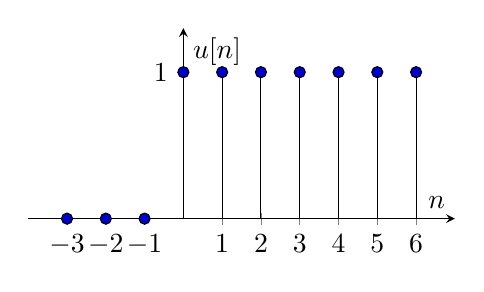
\begin{tikzpicture}
        \begin{axis}[width=7cm,height=4cm,ymin=0,xmin=-4,ymax=1.3,xmax=7,
        xtick={-3,-2,-1,0,1,2,3,4,5,6},
        ytick={0,1,2,3},
        ylabel={$u[n]$},
    xlabel={$n$}, axis lines = center]
   \addplot+[ycomb,color=black] plot coordinates {(-3,0) (-2,0) (-1,0) (0,1) (1,1) (2,1) (3,1) (4,1) (5,1) (6,1)};
\end{axis}
        \end{tikzpicture}
\end{center}
\caption{A discrete-time unit step function.}
\label{fig:dt_ustep}
\end{marginfigure}




\newpage
\section{Exercises: Elementary Signals}

The following exercises cover typical integrals with elementary signals, which you'll encounter in signal processing.

\begin{enumerate}
\item Simplify the following integrals:
  \begin{enumerate}[a)]
    \item
  \begin{equation*}
    \int_{-\infty}^{\infty} \delta(t)e^{i\omega t} dt = ?
  \end{equation*}
      \item

  \begin{equation*}
    \int_{-\infty}^{\infty} \delta(t-\tau)e^{i\omega t} dt = ?
    \end{equation*}
      \item
  \begin{equation*}
    \int_{-\infty}^{\infty} \delta(\omega)e^{-i\omega t} d\omega = ?
    \end{equation*}
      \item
  \begin{equation*}
    \int_{-\infty}^{\infty} \delta(\omega-\omega_0)e^{-i\omega t} d\omega = ?
  \end{equation*}
  \end{enumerate}
\item Show that the integral:
\begin{equation*}
    \int_{-\infty}^{\infty} [u(t+L)-u(t-L)]e^{i\omega t}dt
\end{equation*}
evaluates to:
\begin{equation*}
    \alpha (e^{i\omega L} - e^{-i\omega L})
\end{equation*}
What is $\alpha$?

\item Consider the following integral
\begin{equation*}
    \int_{-\infty}^{\infty}\sin(t-c)\delta(t)dt.
\end{equation*}
For which value of $c$ do we have
\begin{equation*}
    \int_{-\infty}^{\infty}\sin(t-c)\delta(t)dt=0?
\end{equation*}

\item Evaluate the integral
\begin{equation*}
    \int_{-\infty}^{\infty}u(t)u(L-t)\cos(2\pi\omega t)dt.
\end{equation*}



\end{enumerate}

 \ifSpExerciseSol
 \newpage
\section{Suggested solutions: Elementary Signals}

\begin{enumerate}
\item By definition and known properties for the Dirac delta function, we have
$$\int_{-\infty}^{\infty}x(t)\delta(t-\tau)dt=x(\tau).$$

\item[a)]
Using the above we get
$$\int_{-\infty}^{\infty}\delta(t)e^{i\omega t}dt=e^{i\omega\cdot 0}=\underline{\underline{1}}.$$

\item[b)]
Similarly we get
$$\int_{-\infty}^{\infty}\delta(t-\tau)e^{i\omega t}dt=\underline{\underline{e^{i\omega\tau}}}.$$

\item[c)]
If the variable is $\omega$, we have
$$\int_{-\infty}^{\infty}\delta(\omega)e^{-i\omega t}d\omega=\underline{\underline{1}},$$
by the same reasoning as a). 

\item[d)]
$$\int_{-\infty}^{\infty}\delta(\omega-\omega_{0})e^{-i\omega t}d\omega=\underline{\underline{e^{-i\omega_{0}t}}}.$$

\item Consider the integral
$$\int_{-\infty}^{\infty}[u(t+L)-u(t-L)]e^{i\omega t}dt.$$
This corresponds to a rectangular function with height $1$ and width $2L$ centered around $0$. Thus, the integral can be simplified to
$$\int_{-\infty}^{\infty}[u(t+L)-u(t-L)]e^{i\omega t}dt=\int_{-L}^{L}[u(t+L)-u(t-L)]e^{i\omega t}dt.$$
The function $u(t+L)-u(t-L)\equiv 1$ on the interval $[-L,L]$, hence
$$\int_{-L}^{L}[u(t+L)-u(t-L)]e^{i\omega t}dt=\int_{-L}^{L}e^{i\omega t}dt=\left[\frac{1}{i\omega}e^{i\omega t}\right]_{-L}^{L}=\frac{1}{i\omega}(e^{i\omega L}-e^{-i\omega L}).$$
Therefore, $\alpha=\frac{1}{i\omega}$.

\item Using the properties of the Dirac delta function we have
$$\int_{-\infty}^{\infty}\sin(t-c)\delta(t)dt=\sin(0-c)=\sin(-c)=-\sin(c).$$
This evaluates to $0$ for $c=\pi n$ where $n\in\mathbb{Z}$. Thus, $c$ has to be $c=\pi n$.

\item The function $u(t)u(L-t)$ corresponds to a rectangular function of length $L$ and is $0$ whenever $t<0$ and $t>L$ and $1$ if $0<t<L$, therefore the integral can be written as
$$\int_{-\infty}^{\infty}u(t)u(L-t)\cos(2\pi\omega t)dt=\int_{0}^{L}\cos(2\pi\omega t)dt=\frac{1}{2\pi\omega}\left[\sin(2\pi\omega t)\right]_{t=0}^{t=L}=\frac{1}{2\pi\omega}\sin(2\pi\omega L).$$


\end{enumerate}
 \fi
\fi

\ifSpSin
\chapter{Sinusoidal Signals}
\newthought{A \index{complex sinusoidal signal}{complex sinusoidal signal} is the elementary building block of the Fourier decomposition of a signal}. This signal is fully determined by three parameters:
\index{amplitude}{amplitude} $A \in \mathbb{R}_{\ge 0}$, \index{phase}{phase} $\phi \in \mathbb{R}$ (rad), and
\index{angular frequency}{angular frequency} $\omega \in \mathbb{R}$ (rad/s).
\begin{equation}
\boxed{
z(t) = A e^{i(\omega t + \phi)} = A e^{i\phi} e^{i\omega t} = X e^{i\omega t}.
}
\end{equation}
It is possible to combine phase and amplitude as one complex constant $X = Ae^{i\phi} \in \mathbb{C}$. This constant contains information about the amplitude and phase of the signal. $X$ is often referred to as a \emph{\index{phasor}{phasor}}.

\begin{marginfigure}
\begin{center}
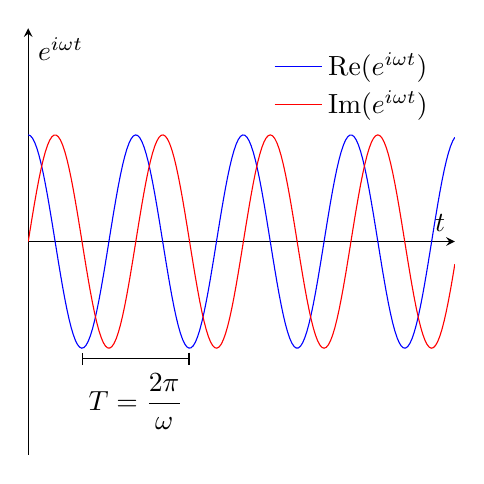
\begin{tikzpicture}
	\begin{axis}[domain=0:(2*6.23),
        width=7cm,
        height=7cm,
        ticks=none,
        axis lines = center,
        ymax=2,
        ymin=-2,
        samples=200,
        legend pos=north east,
        legend style={draw=none},
        xlabel={$t$},
        ylabel={$e^{i\omega t}$}]
    \addplot[blue] {cos(2*deg(x))};
    \addplot[red] {sin(2*deg(x))};

    \node at (axis cs:3.14,-1.5) {$\displaystyle{T=\frac{2\pi}{\omega}}$};   
    \addplot [dimen] plot coordinates {(1.57,-1.1) (4.71,-1.1)};
    
    \legend{$\mathrm{Re}(e^{i\omega t})$,$\mathrm{Im}(e^{i\omega t})$}
    \end{axis}
\end{tikzpicture}
\end{center}
\caption{A complex sinusoidal signal is the basic building block (basis function) in a Fourier decomposition of a signal. The fundamental period $T=2\pi/\omega$
of this signal is also shown.}
\label{fig:complex_sinusoid}
\end{marginfigure}

\begin{marginfigure}
\begin{center}
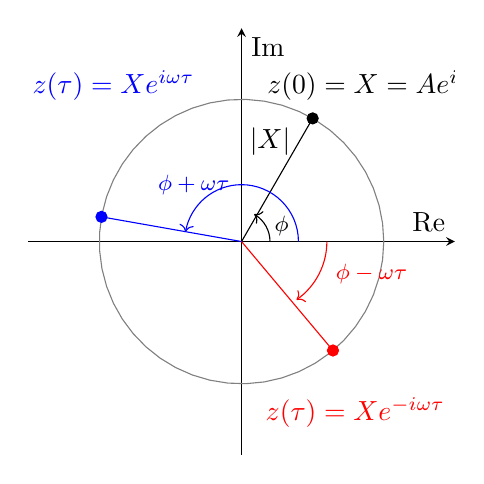
\begin{tikzpicture}
	\begin{axis}[axis equal, disabledatascaling,
    ymin=-1.5,xmin=-1.5,ymax=1.5,xmax=1.5, ticks=none,
    xlabel=$\mathrm{Re}$, ylabel=$\mathrm{Im}$, axis lines = center,
    width=7cm, height=7cm] \addplot
    [gray,domain=0:2*pi,samples=50]({cos(deg(x))},{sin(deg(x))});
    
    \addplot [black, mark = *] coordinates {( {cos(60)}, {sin(60)} )} {};   
     \addplot [black] coordinates { (0,0) ( {cos(60)}, {sin(60)} ) };

    \addplot [blue, mark = *] coordinates {( {cos(170)}, {sin(170)} )} {};   
     \addplot [blue] coordinates { (0,0) ( {cos(170)}, {sin(170)} ) };

   \addplot [red, mark = *] coordinates {( {cos(-50)}, {sin(-50)} )} {};   
     \addplot [red] coordinates { (0,0) ( {cos(-50)}, {sin(-50)} ) };

  \draw[draw=black, ->] (axis cs:0.2,0) arc [radius=0.4cm,start angle=0,end angle=60]
  node[midway,right,inner sep=3pt,font={\footnotesize}]{$\phi$};

%  \draw[draw=blue] (axis cs:1,0) arc [radius=0.5cm,start angle=60,end angle=120]
%  
\draw [blue, ->] (axis cs:0.4,0.0) arc [radius=0.4,start angle=0,end angle=170]
node[midway,left,inner sep=6pt,font={\footnotesize}]{$\phi+\omega \tau$};

\draw [red, ->] (axis cs:0.6,0.0) arc [radius=0.5,start angle=0,end angle=-55]
node[midway,right,inner sep=6pt,font={\footnotesize}]{$\phi-\omega \tau$};

 \node at (axis cs:0.9,1.1) {$z(0)=X=Ae^{i\phi}$};

 \node at (axis cs:0.2,0.7) {$|X|$};

 \node[blue] at (axis cs:-0.9,1.1) {$z(\tau)=X e^{i\omega \tau}$};
 \node[red] at (axis cs:0.8,-1.2) {$z(\tau)=X e^{-i\omega \tau}$};
\end{axis}
\end{tikzpicture}
\end{center}
\caption{A complex sinusoidal signal on the complex plane can be seen as a point moving around a circle. For positive frequencies, the point rotates around the circle in counterclockwise direction. For negative frequencies, the rotation is clockwise.}
\label{fig:rotating_phasor}
\end{marginfigure}

Using Euler's formula, we can express the \index{complex sinusoidal signal}{complex sinusoidal signal} as a function of \index{$\cos$}{$\cos$} and \index{$\sin$}{$\sin$}:
\begin{equation}
Ae^{i(\omega t + \phi)}= A[\cos(\omega t + \phi) + i \sin(\omega t + \phi)].
\end{equation}
With this formulation, it is apparent that the real and imaginary components are identical sinusoidal signals, which are 90 degrees out of phase with each other, because we know that $\cos(\theta)
= \sin(\theta + \pi/2)$. Figure \ref{fig:complex_sinusoid} shows an example of a complex sinusoidal signal.

You can also think of a complex sinusoidal signal as a point on the complex plane, which rotates around in a circle around the origin. This is sometimes referred to as the \emph{rotating phasor}. The radius of the circle is the amplitude of the signal $A=|X|$. At $t=0$, the point is at a phase angle of $\phi$. This phase angle as a function of time is given by $\phi + \omega t$ and determines the position of the point on the circle at a given time. If $\omega>0$, then the point moves counterclockwise around the circle when the value of $t$ increases. If $\omega < 0$, then the point moves
in the clockwise direction around the circle as the the value of $t$ increases. Figure \ref{fig:rotating_phasor} depicts this concept.

This might at first seem like an unnecessarily complicated way to express a sinusoidal signal, but this representation often simplifies the mathematics. For example, it is in most cases much easier to algebraically work with the function $\frac{1}{2}(e^{i\phi}e^{i\omega
t}+e^{-i\phi}e^{-i\omega t})$ than it is with $\cos(\omega t + \phi)$, even though they are the same thing.

You'll also see later on, that a complex sinusoidal signal is
an \emph{\index{eigenfunction}{eigenfunction}} for any linear
time-invariant operator. It allows us to characterize the properties of a linear time-invariant system just by simply investigating what effect the system has on a complex sinusoidal signal. If we spend the effort to learn how to use a complex sinusoidal signal, then we'll know everything there is to know about linear time-invariant systems!

\newthought{Real valued sinusoidal signals can be related to complex sinusoidal signals}. Using the inverse Euler relationship, we can express a real valued sinusoidal signal of some amplitude, angular frequency, and phase. By taking the real or imaginary part of a complex sinusoidal signal, we obtain a cosine or sine signal.

Using the earlier definition of a complex sinusoidal signal, we find that:
\begin{align}
\Re{z(t)} &= \frac{1}{2}\left[X e^{i\omega t} + X^* e^{-i\omega t}\right] = A\cos(\omega t + \phi) \label{eq:resignal} \\
\Im{z(t)} &= \frac{1}{2i}\left[X e^{i\omega t} - X^* e^{-i\omega t}\right] = A\sin(\omega t + \phi) \label{eq:imsignal}
\end{align}
This tells us that a real valued sinusoidal signal with angular frequency $\omega$ is a sum of a positive and negative frequency complex sinusoidal signal with angular frequencies $\pm\omega$. Note that the sign of the phase angles of the two complex sinusoidal signals are also $\pm\phi$.

\newthought{Angular frequency $\omega$} of a complex sinusoidal signal determines how many radians the phase of the signal advances per unit of time. If the unit of time is seconds, the angular frequency has units of \emph{radians per second} (rad/s).

It is possible to relate angular frequency to frequency $f$ in units of cycles per time unit, i.e., how many times does the point whose position is indicated by the complex sinusoidal signal rotate around the circle per unit of time:
\begin{equation}
\boxed{\omega = 2\pi f}
\end{equation}
If the unit of time is seconds, then the unit of frequency $f$ is hertz (Hz or 1/s). Sometimes \emph{cycles per second} is indicated as the unit for frequency. 

I will try to consistently use the name \emph{angular frequency} and symbol $\omega$ when referring to a frequency that is in units of radians per unit of $t$. I will use the name \emph{\index{frequency}{frequency}} and the symbol $f$ when referring to the frequency that is in units of cycles
per unit of $t$. In some cases, when I am talking about frequency in general and it does not matter what the units are, I will drop the word angular and just talk about frequency.

It is unfortunate that these two competing units exist. It
occasionally causes confusion even for people who have worked with signals for many years!  It is not unusual to find a factor of $2\pi$ missing or unnecessarily added in a textbook that is discussing the frequency of a signal.

Throughout these lecture notes, we will most of the time call the independent variable $t$ of a one dimensional signal time and assign it units of seconds. However, the physical units of $t$ do not necessarily have to be seconds, and $t$ does not have to denote time.

For example, if the units of $t$ were e.g., distance in meters, then we would have an angular frequency $\omega$ that is in units of radians per meter, and frequency $f$ that is in units of cycles per meter. In physics, a spatial frequency is typically called a \emph{\index{wavenumber}{wavenumber}}. It is customary to use the symbol $k$ for angular wavenumber and the Greek letter $\nu$ for linear wavenumber. These types of spatial frequencies are often encountered when dealing with propagating waves. There is an example at the end of this chapter on this topic.

\newthought{Complex and real valued sinusoidal signals} are periodic. The definition of a \index{periodic function}{periodic function} requires that the function repeats after a certain time period $T$ for all values of $t$:
\begin{equation}
\boxed{z(t) = z(t+ n T).}
\end{equation}
where $n \in \mathbb{Z}$ and $T \in \mathbb{R}_{>0}$.  

The smallest possible positive non-zero value of $T$ is called the \emph{\index{fundamental period}{fundamental period}} of the function. 

In the case of complex sinusoidal signals, the definition of periodicity yields:
\begin{align}
Ae^{i (\omega t + \phi)}= Ae^{i (\omega (t+T) + \phi)} = Ae^{i (\omega t+ \omega T + \phi)}
\end{align}
By definition, we know that a complex sinusoidal signal is
$2\pi$-periodic, in other words
\begin{equation}
Ae^{i\theta}=Ae^{i(\theta+2\pi k)}
\end{equation}
for $k\in\mathbb{Z}$. By setting $\theta = \omega t +\phi$, this implies that $\omega T = 2\pi k$.

In order to look for the smallest value of $T$, we inspect the case where $k=1$, from which it follows that the fundamental period is:
\begin{equation}
\boxed{T = \frac{2\pi}{\omega} = \frac{1}{f}.}
\end{equation}
The fundamental period for a complex sinusoidal signal is shown in Figure \ref{fig:complex_sinusoid}.

\newthought{Multiple complex sinusoidal signals with the same frequency but possibly different phases and amplitudes can be added together to form one complex sinusoidal signal}. This is sometimes referred to as the \emph{\index{phasor summation}{phasor summation}}\sidenote{The signal $A e^{i\phi}e^{i\omega t}$ is called a phasor if $A$, $\phi$, and $\omega$ have no time dependence.} property.

Let us assume that we have $N$ complex sinusoidal signals. Each one of these signals has the same angular frequency $\omega$ but different phases $\phi_n$ and amplitudes $A_n$. If we add these together, we get one complex sinusoidal signal with an amplitude $A$ and phase $\phi$:
\begin{equation}
\sum_{n=1}^N A_n e^{i(\omega t + \phi_n)} = A e^{i (\omega t + \phi)}
\end{equation}
This is relatively easy to see. Let's define $X_n = A_n e^{i\phi_n}$, which allows us to rewrite the sum in the following form:
\begin{align}
\sum_{n=1}^N A_n e^{i(\omega t + \phi_n)} &= \sum_{n=1}^N X_n e^{i\omega t} \\
&= \underbrace{\left(\sum_{n=1}^N X_n\right)}_{X} e^{i\omega t} \\
&= X e^{i\omega t}\\
&= |X| e^{i\angle X} e^{i\omega t}\\
&= A e^{i \phi} e^{i\omega t}
\label{eq:sum_sinusoids}
\end{align}
Here $X=\sum_n X_n$ is just a sum of constant valued complex numbers that contain information about the phases and amplitudes of the individual complex sinusoids.

\newthought{Multiplying two complex sinusoidal signals together is equivalent to a shift in frequency and phase}.
Consider two complex sinusoidal signals with angular frequencies $\omega_1$ and $\omega_2$, and phase angles $\phi_1$ and $\phi_2$. For the sake of simplicity, we'll assume that both signals are unit amplitude:
\begin{align}
z_1(t) &=  e^{i(\omega_1 t + \phi_1)}\\
z_2(t) &=  e^{i(\omega_2 t + \phi_2)}
\end{align}
Multiplying together these two signals $z_3(t) = z_1(t)z_2(t)$ we get:
\begin{equation}
\boxed{e^{i(\omega_3 t + \phi_3)}  = e^{i[(\omega_1 + \omega_2) t + (\phi_1+\phi_2)]}}
\label{eq:freqmix}
\end{equation}
The resulting signal $z_3(t)$ is a complex sinusoid, at a new frequency: $\omega_3 = \omega_1 + \omega_2$ and phase $\phi_3=\phi_1+\phi_2$.

This property is one of the elementary operations in signal
processing. For example, we'll use multiplication of two complex sinusoidals signals later on as part of the proof of the Shannon-Nyquist sampling theorem.

The frequency shift property is also widely used in radio engineering and telecommunications to shift high frequency signals to lower frequencies and vice versa. This operation is called downconversion or upconversion in radio engineering terminology.

\newthought{It is possible to extend the concept of a complex sinusoidal signal into multiple dimensions}. For example, a \index{two dimensional complex sinusoidal
signal}{two dimensional complex sinusoidal
signal} would be of the form:
\begin{equation}
z(x,y) = A e^{i\phi} e^{i k x} e^{i \ell y}.
\end{equation}
Here $k$ and $\ell$ are the angular frequencies in the $x$ and $y$ directions.

In the last example\sidenote{I couldn't resist using this nice example, even though this course is about 1d signals.} of this chapter, we'll show how to use a two-dimensional complex sinusoidal signal to derive the plane wave solution of electromagnetic waves propagating in free space from Maxwell's equations.

\newthought{A time-shift is equivalent to a phase shift for a complex sinusoidal signal}.
Let's investigate a time-shift system, which shifts time by a constant $\tau$:
\begin{equation}
y(t) = \mathcal{T}\{x(t)\} = x(t-\tau),
\end{equation}
which means that the output signal at time $t$ is the same as the input signal at time $t-\tau$. One could also say that the output signal is delayed by a time constant $\tau$.

\pgfplotsset{
    dirac/.style={
        mark=triangle*,
        mark options={scale=2},
        ycomb,
        scatter,
        visualization depends on={y/abs(y)-1 \as \sign},
        scatter/@pre marker code/.code={\scope[rotate=90*\sign,yshift=-2pt]}
    }
}
\begin{marginfigure}[-2cm]
\begin{center}
\begin{tikzpicture}
\begin{axis}[width=7cm,height=4cm,ymin=0,xmin=-0.5,ymax=1.1,xmax=1.5,         
        yticklabels={,,},
        xtick={0,1},
        xticklabels={$0$,$\tau$},
        xlabel=$t$,
        axis y line=middle, axis x line=bottom] 
%        , axis lines = center]
\addplot +[dirac,blue] coordinates {(1,1)};
\node at (axis cs:0.75,1) [below, blue, font={\footnotesize}]{$\delta(t-\tau)$};
\addplot +[dirac,red] coordinates {(0,1)};
\node at (axis cs:-0.15,1) [below, red, font={\footnotesize}]{$\delta(t)$};
\end{axis}
\end{tikzpicture}
\end{center}
\caption{Time-shifted unit impulse. The time-shift system $y(t)=x(t-\tau)$ will delay the input signal by $\tau$.}
\label{fig:uparrow2}
\end{marginfigure}

For example, if $x(t)=\delta(t)$, then the location of the only non-zero valued peak in the input signal will be at $t=0$. If we delay the signal by $\tau$, then $y(t)=\delta(t-\tau)$ and the peak will now occur at $t=\tau$.

What does the time-delay system do to a complex sinusoidal signal? If the input signal is $x(t) = e^{i(\omega t + \phi)}$, the output becomes:
\begin{align}
y(t) = \mathcal{T}\{e^{i(\omega t + \phi)}\} &= e^{i[\omega (t-\tau) + \phi]}\\
&=  e^{i(\omega t + \phi - \omega \tau)}\\
&=  e^{-i\omega \tau}x(t)
\end{align}
The output of the time-shift system for a complex sinusoidal signal is
the input signal multiplied by $e^{-i\omega \tau}$. In other words,
phase shifted by $-\omega \tau$ radians. There is a linear dependence
of phase shift with frequency as shown in
Figure \ref{fig:timeshift_phase}.

\begin{marginfigure}
\begin{center}
\begin{tikzpicture}
	\begin{axis}[domain=(-10):(10),samples=200, legend
    style={draw=none,at={(.99,.1)},anchor=south east},
    xlabel={$\omega$},
    ylabel={$-\omega \tau$},
    axis x line=center,
    axis y line=middle,
    ytick={0,1.5708,3.14159,4.7123889,6.23},
    yticklabels={$0$,$\frac{\pi}{2}$,$\pi$,$\frac{3\pi}{2}$,$2\pi$},
    width=6cm,
    height=6cm,
    ]

\addplot[blue] {-0.5*x};
%\legend{Phase shift $\theta=\omega \tau$}
\end{axis}
\end{tikzpicture}
\end{center}
\caption{Phase shift introduced to a complex sinusoidal signal by a time-shift system. The phase shift caused by a constant time shift is linearly dependent on angular frequency.}
\label{fig:timeshift_phase}
\end{marginfigure}

Because of the $2\pi$-periodicity of the complex sinusoidal signal,
the phase shift introduced by a certain time delay is not
unique. There are infinitely many time shifts that can cause a certain
phase shift at a fixed frequency.

Let's say that a complex sinusoidal signal is phase shifted by phase
$\theta$. Due to the $2\pi$ periodicity, we have to consider all
values $\theta + 2\pi k$ with $k\in\mathbb{Z}$. If we attribute this
phase shift only to a time-delay, then the following relationship holds
\begin{equation}
e^{i (\theta+2\pi k)} = e^{-i \omega \tau}.
\end{equation}
This means that all of the time delays that could have caused a phase shift $\theta$ are:
\begin{equation}
\tau = -\omega^{-1}(\theta+2\pi k).
\end{equation}
This problem is sometimes called phase-time ambiguity.

Sometimes it is possible to solve this ambiguity by making the assumption that the true value of the time-shift is within a certain interval $\tau_{\mathrm{min}} < \tau < \tau_{\mathrm{max}}$ and find a unique solution for $\tau$.

Another possible solution to the phase-time ambiguity is to measure the rate-of-change of the phase as a function of frequency:
\begin{equation}
\frac{d\theta}{d\omega} = -\tau.
\end{equation}
This type of a measurement is used by devices called network analyzers for measuring the length of a cable. This principle is also used in the radio astronomical method called very long baseline interferometry (VLBI) to determine the relative time delay between a point-like radio emission source and two different radio telescopes.

\begin{marginfigure}
\begin{center}
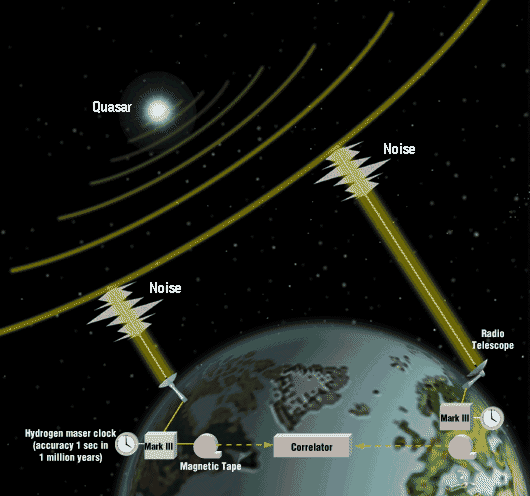
\includegraphics[width=\textwidth]{ch06/figures/vlbi.png}
\end{center}
\caption{In radio astronomy, the relative time delay between two Earth-based radio telescopes and a point like radio emission source is determining the rate of change of the relative phase as a function of frequency. Figure: NASA GFSC.}
\label{fig:vlbi_concept}
\end{marginfigure}



\section{Example: Very long baseline interferometry}
A point-like radio star emits a signal across a broad range of frequencies. This means that we can observe the signal originating from the radio star with multiple angular frequencies $\omega$. We can denote the signal originating from the star at a certain frequency with:
\begin{equation}
z(t,\omega) = A(\omega) e^{i\phi(\omega)} e^{i\omega t}
\end{equation}
Here $A(\omega) \in \mathbb{R}_{\ge 0}$ is the amplitude and $\phi(\omega)$ is the phase of the signal at angular frequency $\omega$. Because the signal is generated by an enormous collection of charged particles (primarily electrons) in an accelerating motion, the amplitudes and phases are random variables.

If we measure the signal originating from the radio star at two different places with a radio telescope simultaneously, the time of arrival of the signal between the two telescopes will differ by $\tau$ due to geometry (see Figure \ref{fig:vlbi_concept}). It is this value of $\tau$ that is often of interest, when e.g., estimating the orientation of Earth relative to the stars. 

Let's denote the signal received with telescope 1 with $z_1$ and the signal received with telescope 2 with $z_2$:
\begin{align}
z_1(t,\omega) &= A(\omega) e^{i\phi(\omega)} e^{i\omega t} \\
z_2(t,\omega) &= A(\omega) e^{i\phi(\omega)} e^{i\omega (t-\tau)}
\end{align}
We'll assume that $z_1$ is the same signal as $z_2$ with only one exception, the signal $z_2$ is delayed by time constant $\tau$ due to the receiver being further away from the source of the signal\sidenote{For radio signals, we need the radio source to be in the Fraunhofer far-field in order for this to be valid.}.

In order to determine the value $\tau$, we can use the following operation:
\begin{equation}
z_1(t,\omega)z_2^*(t,\omega) = |A(\omega)|^2 e^{i\omega \tau} 
\end{equation}
The random phase $\phi(\omega)$ cancels out with this operation, as well as the oscillating term $\omega t$. The phase of this cross-product only depends on frequency and time shift $\tau$:
\begin{equation}
\angle z_1(t,\omega)z_2^*(t,\omega) = \theta(\omega)= \omega \tau
\end{equation}
If we measure the cross-product $z_1(t,\omega)z_2^*(t,\omega)$ across a sufficiently wide range of frequencies, we can estimate $\tau$ using:
\begin{equation}
\frac{d\theta}{d\omega}= \tau
\end{equation}
This is a very simplified description of how the very long baseline interferometry technique used in radio astronomy and geodesy allows us to precisely measure the relative difference in time of arrival of a signal originating from a point-like radio source when measured with two different radio receivers.

\if 0
\section{Python example: plotting sinusoidal signals}

The following example will get you started with Python and signal
processing. It is a sort of a \index{Hello World}{Hello World}, which plots a sinusoid.
\begin{lstlisting}[language=Python]
import numpy as n
import matplotlib.pyplot as plt

# time vector (1000 samples per second) one second duration
t=n.arange(1000)/1000.0
# create a 10 Hz sinusoidal signal with amplitude 10
x=10.0*n.cos(2.0*n.pi*10.0*t)
# create a 10 Hz sinusoidal signal with amplitude 5, 
# time shifted by 0.02 s
xd=5.0*n.cos(2.0*n.pi*10.0*(t+0.02))

plt.plot(t,x,label="$x(2\pi 10 t)$")
plt.plot(t,xd,label="$x(2\pi 10(t+0.02))$")

plt.legend()
plt.show()
\end{lstlisting}
\fi

\section{Python example: shifting in frequency}

The following Python example demonstrates in practice
Equation \ref{eq:freqmix} which tells us that when multiplying two complex sinusoidal signals together, the resulting signal will have a frequency corresponding to the sum of the two frequencies of the multiplied signals.

\lstinputlisting[language=Python,caption={\texttt{005\_mixing/mixing.py}},label=lst:mixing_ex]{ch06/code/mixing.py}

\section{Example: Electromagnetic waves}
\label{waveeq}

This example will show that complex sinusoidal signals are a useful mathematical tool also for solving differential equations by deriving a plane wave solution of \index{electromagnetic waves}{electromagnetic waves} from \index{Maxwell's equations}{Maxwell's equations}.

Don't worry if you are not familiar with these equations. I mainly want you to pay attention to how the differential equation is solved for a plane wave using a \index{two-dimensional complex sinusoidal signal}{two-dimensional complex sinusoidal signal} $\vec{E}(x,t)=\hat{y}E_0 e^{i k x}e^{i\omega t}$. Because the exponential function is easy to differentiate, it is easy to apply this type of a function for solving differential equations.

Assuming that there are no currents ($\vec{J}=0$) or space charges ($\rho=0$), \index{Maxwell's equations}{Maxwell's equations} are as follows:
\begin{align}
\nabla \cdot \vec{E} &= 0 \\
\nabla \cdot \vec{B} &= 0 \\
\nabla \cross \vec{E} &= -\frac{\partial \vec{B}}{\partial t} \label{eq:faraday}\\
\nabla \cross \vec{B} &= \epsilon_0 \mu_0 \frac{\partial \vec{E}}{\partial t} \label{eq:maxwell}
\end{align}
If we curl Faraday's law, we get:
\begin{align}
\nabla \cross (\nabla \cross \vec{E}) &= -\frac{\partial }{\partial t}\nabla \cross \vec{B}
\end{align}
If we then use the vector identity
$\nabla \cross (\nabla \cross \vec{E}) = \nabla(\nabla \cdot \vec{E}) - \nabla^2 \vec{E}$ and include Gauss' law for electric field $\nabla \cdot \vec{E} = 0$ in the case when there are no charges, we get
\begin{align}
\nabla^2 \vec{E} &= \frac{\partial }{\partial t}\nabla \cross \vec{B}
\end{align}
If we now insert insert Maxwell-Ampere's law (Equation \ref{eq:maxwell}) into Faraday's
law (Equation \ref{eq:faraday}), we get:
\begin{align}
\frac{\partial^2 \vec{E}}{\partial t^2} - \frac{1}{\mu_0 \epsilon_0} \nabla^2 \vec{E} &= 0.
\end{align}
This type of equation is called a \index{wave equation}{wave equation}. You can derive the same equation also for the magnetic field, but we are not going to do that here.

Now let us assume that a solution to the wave equation is of the form:
\begin{equation}
\vec{E}(x,t)= E_0 \hat{y} e^{-i k x}e^{i\omega t}
\label{efieldplanewave}
\end{equation}
Here $E_0 \in \mathbb{C}$ is a complex number that determines the amplitude and phase of the electric field. The term $\hat{y}$ is a unit vector in the y-axis direction. In other words, a plane wave, where the electric field in the y-z plane is constant valued. The electric field only changes as a function of position in the $x$-axis as a function of time $t$.

\begin{figure}
\begin{center}
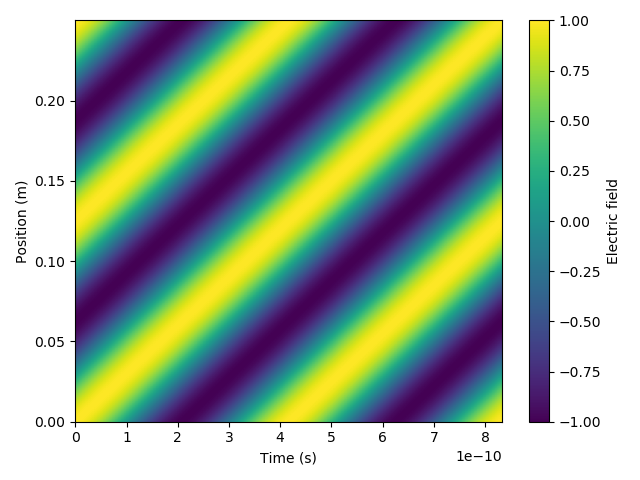
\includegraphics[width=\textwidth]{ch06/figures/em_plane_wave.png}
\end{center}
\caption{A plane wave solution to Maxwell's equations, describing propagation of electromagnetic waves in space and time. The script that produced this plot is \texttt{007\_2dwave/em\_plane\_wave.py}. }
\label{fig:planewave}
\end{figure}

It is easy to differentiate a complex exponential function twice in space and time. Remember that the \index{Laplacian operator}{Laplacian operator}, which is a linear system, is defined as:
\begin{equation}
\nabla^2 = \frac{\partial^2}{\partial x^2} + \frac{\partial^2}{\partial y^2} +\frac{\partial^2}{\partial z^2} 
\end{equation}
Because the electric field is constant in the y-z plane, only the second derivative in the x-direction remains. Using the two dimensional plane wave formulation of Equation \ref{efieldplanewave}, we can see that
\begin{align}
\frac{\partial ^2 \vec{E}}{\partial t^2} &= -\omega^2 \vec{E}(x,t) \\
\nabla^2 \vec{E} &= -k^2 \vec{E}(x,t).
\end{align}
And therefore, the wave equation becomes:
\begin{align}
\frac{\partial^2 \vec{E}}{\partial t^2} - \frac{1}{\mu_0 \epsilon_0} \nabla^2 \vec{E} &= 0 \\
(c^2k^2-\omega^2) \vec{E}(x,t) &= 0 \label{eq:disp_relation}
\end{align}
I've taken the liberty of changing the constant $c =
(\mu_0\epsilon_0)^{-1/2}$ for reasons that will become apparent soon. The constant $\mu_0$ is permeability of free space, and $\epsilon_0$ is permittivity of free space. The value of $c \approx 3\cdot 10^{8}$ m/s.

In order for the two dimensional complex sinusoidal signal to be consistent with Maxwell's equations, either $E(x,t)=0$ or $c^2k^2-\omega^2 = 0$. The trivial solution $E(x,t)=0$ is not very interesting, as there would be no electric field. The latter describes a solution with a non-zero electric field, as long as the following relationship:
\begin{equation}
k = \pm \frac{\omega}{c}
\end{equation}
is satisfied. This means that the following two-dimensional signal is a solution to the Maxwell's equations:
\begin{align}
\vec{E}(x,t) &= E_0 \hat{y} e^{-i (\omega/c) x} e^{i\omega t} \\
             &= E_0 \hat{y} e^{-i 2\pi \lambda^{-1} x} e^{i 2\pi f t} 
\end{align}
Here, I've used the relation $2\pi f = \omega$. I've also used the wavelength of the electromagnetic wave, which is $\lambda = c/f$. In other words, we have used a two dimensional complex sinusoidal signal and the Maxwell's equations to describe how electromagnetic waves propagate in space and time.

I am showing the real part of the plane wave solution in
Figure \ref{fig:planewave}. In this case, the frequency is chosen to
be $f=2.4$ GHz, which is the frequency typically used by microwave
ovens and wireless internet (which you are probably using right
now). Try to figure out what is the velocity that a region of constant
phase propagates in the positive x-axis direction at.




\newpage
\section{Exercises: Sinusoidal Signals}

Hint: You can often write a Python program to verify your result if you are not sure it is correct!

\begin{enumerate}

\item You may have heard somebody say that noise cancelling headphones
  rely on playing an audio signal where each spectral component of the
  signal is perfectly ``out of phase'' with the input signal. Consider
  a noise source that is sinusoidal and described by the following
  equation:
\begin{equation}
x_{\mathrm{noise}}(t) = \cos(\omega t + \phi).
\end{equation}
Your noise cancelling system can generate a signal
$x_{\mathrm{cancel}}(t)$ with the same amplitude and frequency, but a different phase:
\begin{equation}
x_{\mathrm{cancel}}(t) = \cos(\omega t + \phi_c)
\end{equation}
What value of $\phi_c$ results in perfect cancellation
\begin{equation}
  x_{\mathrm{cancel}}(t) + x_{\mathrm{noise}}(t) = 0?
\end{equation}

\item Prove that:
\begin{equation}
A\cos(\omega t + \phi) = a\cos(\omega t) + b\sin(\omega t). 
\end{equation}
How is $A$ and $\phi$ related with $a$ and $b$? Do this by converting the cosine and sine signals to complex sinusoidal signals (Equations \ref{eq:resignal} and \ref{eq:imsignal}). Use the phasor summation property found in Equation \ref{eq:sum_sinusoids}.

The representation of the form $a\cos(\omega t) + b\sin(\omega t)$ is often preferred over $A\cos(\omega t + \phi)$ when estimating the phase and amplitude of a real valued sinusoidal signal from noisy measurements, because we get a set of linear equations with two unknown constants $a$ and $b$.

\item Consider the following signal, which consists of two sinusoidal signals multiplied with one another:
\begin{equation}
x(t) = \cos(\omega_1 t)\sin(\omega_2 t).
\end{equation}
Show that it is possible to express this signal in the form:
\begin{equation}
x(t) = a \sin (\omega_3 t) + b \sin(\omega_4 t).
\end{equation}
What is the value of $a$, $b$, $\omega_3$, and $\omega_4$?


\item The electromagnetic wave example demonstrated that a two-dimensional complex sinusoidal signal of the form:
\begin{equation}
    \vec{E}(x,t) = \hat{y}E_0 e^{i k x} e^{i \omega t}
\end{equation}
is a solution to the Maxwell's equation in free space.

You task is to show that a real-valued solution $\mathrm{Re}\{\vec{E}(x,t)\}$ with $\vec{E}(x,t)\ne 0$ is also a solution to the wave equation, so that we know that it is possible to have solutions with a real valued electric field. In other words, show that Equation \ref{eq:disp_relation} holds also in this case.
\if 0
  \begin{equation}
    \mathrm{Re}\{\vec{E}(x,t)\} = \frac{1}{2}\hat{y}\left(E_0 e^{i (\omega/c) x} e^{i \omega t} + E_0^* e^{-i (\omega/c) x} e^{-i \omega t}\right)
  \end{equation}
  also satisfies Maxwell's equation. Hint: You need to verify that
  Equation \ref{eq:disp_relation} holds.
\fi
  \begin{marginfigure}[0cm]
\begin{center}
  \includegraphics[width=\textwidth]{ch06/figures/prism.png}
\end{center}
\caption{Light can be seen as a superposition of electromagnetic waves with different amplitudes, phases, and frequencies. This can be easily visualized in practice with the help of a prism or a diffraction grating.}
\label{fig:prism_ex}
\end{marginfigure}

\item This is a follow-up question to the previous one. Let's say that we had an arbitrary number of solutions to the wave equation with different angular frequencies $\omega_n$ and phasors $E_n$:
\begin{equation}
    \vec{E}(x,t) = \hat{y}\sum_n E_n e^{i (\omega_n/c) x} e^{i \omega_n t}
\end{equation}
Would this still satisfy the Maxwell's equations (i.e., the wave equation)? Can electromagnetic waves be composed of a superposition of two dimensional plane waves of different frequencies (wavelengths, or colors), which each individually satisfy the wave equation?


\item Copy the example program in Listing \ref{lst:mixing_ex} that performs mixing and run it. The example shows how to shift a complex exponential signal with a certain frequency to another frequency. Modify the script in such a way that the resulting complex exponential signal \verb|z_shifted| has a frequency of 42 Hz. Use the plot to verify that the frequency of the signal is approximately 42 Hz.


\item Go back to the guitar amplifier program
  \texttt{003\_guitar/amplifier.py}. We will now add one more
  effect. We'll modify the program so that it implements a modulation effect.

\begin{itemize}
\item[a)] Multiply the clean guitar signal with a 5 Hz sinusoidal signal. Plot the signal.
\begin{lstlisting}[language=Python]
# multiply with sinusoid
x_mod=x*n.cos(2.0*n.pi*time_vec*5.0)
# plot result
plt.plot(time_vec,x_mod)
plt.show()
\end{lstlisting}
\item[b)] Write the output into an audio file and play the
  result. What does the output sound like? 
\begin{lstlisting}[language=Python]
# write compressed output to wav file. 
sio.write("guitar_leslie.wav",sample_rate,x_mod)
\end{lstlisting}

\item[c)] Change the frequency of the modulating sinusoid from 5 Hz to 2.5 Hz. Predict what the audio will sound like. Play the resulting audio to confirm your hypothesis.

\end{itemize}
If you want to reflect on what is going on here, think of the original
audio signal $x(t)$ as something that consists of a sum of sinusoidal
signal components\sidenote{We'll introduce this properly later on}
\begin{equation}
    x(t) = \sum_{n} A_n \cos(\omega_n t + \phi_n)
\end{equation}
When multiplying this signal with a sinusoidal signal of frequency $\omega$, we get a modulated audio signal $y(t)$:
\begin{align}
y(t) &= x(t) \cos(\omega t)\\
  y(t) &= \left[\sum_{n} A_n \cos(\omega_n t + \phi_n)\right] \cos(\omega t).
\end{align}
Each spectral component of signal $x(t)$ gets the same treatment as you already investigated in Exercise 3.

\end{enumerate}

 \ifSpExerciseSol
 % Author: Jørn Olav Jensen

\newpage
\section{Suggested solutions: Sinusoidal Signals}
\begin{enumerate}
  % Exercise 1
  \item If $x_{\text{noise}}(t)=\cos(\omega t+\phi)$ and $x_{\text{cancel}}(t)=\cos(\omega t+\phi_{c})$ and:
        \[ x_{\text{noise}}(t)+x_{\text{cancel}}(t)=0, \]
        then we must have:
        \[ \cos(\omega t+\phi)+\cos(\omega t+\phi_{c})=0, \]
        for all $t$. The phase doesn't depend on $t$, so it is the same for every $t\in\mathbb{R}$, in particular for $t=0$ so:
        \begin{align*}
          \cos(\phi)  & =-\cos(\phi_{c}),     \\
          \cos(\phi)  & =\cos(\pi -\phi_{c}), \\
          \phi+2\pi k & =\pi-\phi_{c}+2\pi l,
        \end{align*}
        for $k,l\in\mathbb{Z}$, which gives $\phi_{c}=\pi-\phi+2\pi(l-k)=\pi-\phi+2\pi m$,
        where $m\in\mathbb{Z}$. Take $m=0$ to obtain a simple solution, which gives $\phi_{c}=\pi -\phi$.
        Hence, the canceling signal must be of the form:
        \[ x_{\text{cancel}}(t)=\cos(\omega t+(\pi-\phi)). \]
        A simple test program to verify this is shown in Listing \ref{cancel}
        with an arbitrary choice of $\omega$, $\phi$ and $m$.
        If the code is run, two signals of opposite amplitude are shown,
        which cancel out when added, as hoped.
        \lstinputlisting[language=Python, caption={Noise canceling signal}, label=cancel, linerange={0-25}]{ch06/code/ex6.1.py}

  % Exercise 2
  \item Have that:
        \[ a\cos(\omega t)+b\sin(\omega t)=\frac{a}{2}(e^{i\omega t}+e^{-i\omega t})+\frac{b}{2i}(e^{i\omega t}-e^{-i\omega t}), \]
        or written out:
        \[ a\cos(\omega t)+b\sin(\omega t)=\frac{a}{2}e^{i\omega t}+\frac{a}{2}e^{-i\omega t}+\frac{b}{2i}e^{i\omega t}-\frac{b}{2i}e^{-i\omega t}. \]
        Using the phasor summation property we have:
        \[ X = \sum_{n}X_{n} = \frac{a}{2}+\frac{b}{2i}=\frac{1}{2}(a-bi), \]
        and
        \[ Y = \sum_{m}Y_{m} = \frac{a}{2}-\frac{b}{2i}=\frac{1}{2}(a+bi). \]
        Then we have that:
        \begin{align*}
          |X| & =\sqrt{\frac{1}{4}(a^{2}+b^{2})}=\frac{1}{2}\sqrt{a^{2}+b^{2}}, \\
          |Y| & =\sqrt{\frac{1}{4}(a^{2}+b^{2})}=\frac{1}{2}\sqrt{a^{2}+b^{2}},
        \end{align*}
        and
        \begin{align*}
          \angle X & =\arctan\left(\frac{-b}{a}\right)=\phi, \\
          \angle Y & =\arctan\left(\frac{b}{a}\right).
        \end{align*}
        Then the whole expression can be rewritten as:
        \begin{align*}
          a\cos(\omega t)+b\sin(\omega t) & =\frac{1}{2}\sqrt{a^{2}+b^{2}}e^{i\phi}e^{i\omega t}+\frac{1}{2}\sqrt{a^{2}+b^{2}}e^{-i\phi}e^{-i\omega t}, \\
                                          & =\frac{1}{2}\sqrt{a^{2}+b^{2}}e^{i(\omega t+\phi)}+\frac{1}{2}\sqrt{a^{2}+b^{2}}e^{-i(\omega t+\phi)},      \\
                                          & =\sqrt{a^{2}+b^{2}}\left[\frac{1}{2}\left(e^{i(\omega t+\phi)}+e^{-i(\omega t+\phi)}\right)\right],         \\
                                          & =\sqrt{a^{2}+b^{2}}\cos(\omega t+\phi),                                                                     \\
                                          & =A\cos(\omega t+\phi).
        \end{align*}
        Here $A=\sqrt{a^{2}+b^{2}}$ and $\phi=-\arctan(b/a)$, where $\arctan(b/a)$
        should give the angle corresponding to which quadrant the point $(a,b)$ lies in the $xy$-plane.

  % Exercise 3
  \item Consider the signal:
        \[ x(t) = \cos(\omega_{1}t)\sin(\omega_{2}t), \]
        which we can write as:
        \[ x(t) = \frac{1}{2}(e^{i\omega_{1}t}+e^{-i\omega_{1} t})\frac{1}{2i}(e^{i\omega_{2}t}-e^{-i\omega_{2}t})=\frac{1}{4i}[e^{i(\omega_{1}+\omega_{2})t}-e^{i(\omega_{1}-\omega_{2})t}+e^{i(-\omega_{1}+\omega_{2})t}-e^{i(-\omega_{1}-\omega_{2})t}]. \]
        Collecting terms we get:
        \begin{align*}
          x(t) & =\frac{1}{4i}[e^{i(\omega_{1}+\omega_{2})t}-e^{-i(\omega_{1}+\omega_{2})t}]+\frac{1}{4i}[e^{i(-\omega_{1}+\omega_{2})t}-e^{-i(-\omega_{1}+\omega_{2})t}], \\
               & =\frac{1}{2}\sin((\omega_{1}+\omega_{2})t)+\frac{1}{2}\sin((\omega_{2}-\omega_{1})t).
        \end{align*}
        This yields the values $a=1/2$ and $b=1/2$, while $\omega_{3}=\omega_{1}+\omega_{2}$ and $\omega_{4}=\omega_{2}-\omega_{1}$.

  % Exercise 4
  \item The plane wave:
        \[ E(x,t) = E_{0}e^{i(kx+\omega t)}\partial_{y} \]
        is a solution to the wave equation. Consider the real part $\Re\{E(x,t)\}$:
        \[ \Re\{E(x,t)\} = \frac{1}{2}[E(x,t)+E^{*}(x,t)]=\frac{1}{2}E_{0}(e^{i(kx+\omega t)}+e^{-i(kx+\omega t)})\partial_{y}=E_{0}\cos(kx+\omega t)\partial_{y}. \]
        Recall that the wave equation is:
        \[ \partial_{t}^{2}E-\frac{1}{\mu_{0}\epsilon_{0}}\nabla^{2}E=0, \]
        which gives:
        \[ -\omega^{2}E_{0}\cos(kx+\omega t)\partial_{y}+\frac{1}{\mu_{0}\epsilon_{0}}k^{2}E_{0}\cos(kx+\omega t)\partial_{y}=E_{0}\left(\frac{1}{\mu_{0}\epsilon_{0}}k^{2}-\omega^{2}\right)\cos(kx+\omega t)\partial_{y}=0, \]
        since $k^{2}c^{2}-\omega^{2}=0$, as $c=\sqrt{1/\mu_0\epsilon_0}$. In conclusion, the signal:
        \[ \Re\{E(x,t)\} = E_{0}\cos(kx+\omega t)\partial_{y}, \]
        is a solution to the wave equation.

  % Exercise 5
  \item If we have an arbitrary number of solutions to the wave equation, each with different
        phasors $E_{n}$ and different angular frequencies $\omega_{n}$. Then a superposition:
        \[ E(x,t) = \sum_{n}E_{n}e^{i(\omega_{n}/c)x}e^{i\omega_{n}t}\partial_{y}, \]
        is also a solution. This follows by the linearity of the wave equation.

  % Exercise 6
  \item The code from the notes has been modified such that the output signal has a frequency of approximately 42.0 Hz.
        \lstinputlisting[language=Python, caption={Adding frequencies}, label=sig42, linerange={0-33}]{ch06/code/ex6.6.py}
        Running the code in Listing \ref{sig42} yields the following output:
        \begin{figure}[h!]
          \centering
          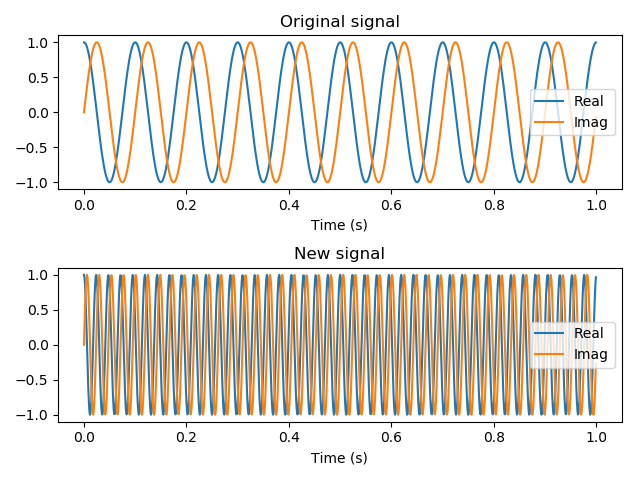
\includegraphics[scale=1.0]{ch06/figures/ex6a.png}
          \caption{Signal with 42 Hz frequency}
        \end{figure}

  % Exercise 7
  \item The following code is a modification that multiplies the signal with a periodic 5.0 Hz signal:
        \begin{itemize}
          % Exercise 7a)
          \item[a)] Listing \ref{sig42_mod} provides a suggested solution.
                \lstinputlisting[language=Python, caption={Modifying signals}, label=sig42_mod, linerange={0-23}]{ch06/code/ex6.7a.py}
                Running Listing \ref{sig42_mod} produces Figure \ref{fig:ex6b}.
                \begin{figure}[h!]
                  \centering
                  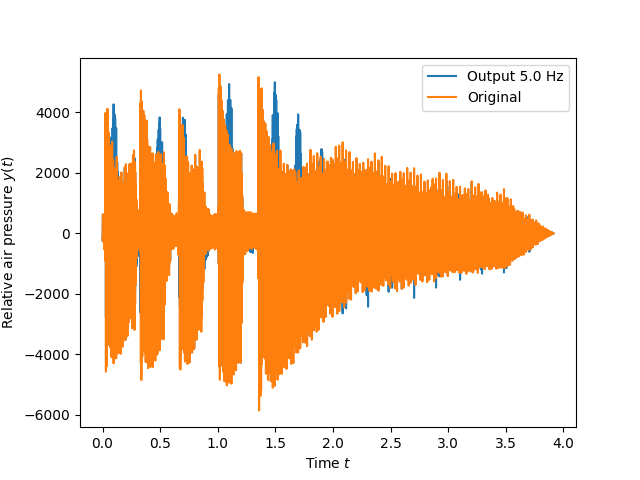
\includegraphics[width=12.5cm, height=9.5cm]{ch06/figures/ex6b.png}
                  \caption{Original and modified guitar signal}
                  \label{fig:ex6b}
                \end{figure}

          % Exercise 7b)
          \item[b)]
                Adding the following code to Listing \ref{sig42_mod} will save the result as an audio file.
\begin{lstlisting}[language=Python, caption=Saving an audiofile, label=save_audio]
out = 0.9*out/np.max(np.abs(out)) 
    
# Multiply the signals.
out2 = x*n.cos(2.0*n.pi*time_vec*2.5)
    
# Write compressed output to wav file.
sio.write("guitar_leslie.wav", sample_rate, np.array(out, dtype=np.float32))
\end{lstlisting}
                Listening to the audio file, we hear that the guitar sound has a wavy oscillating effect.

          % Exercise 7c)
          \item[c)]
                Based on the previous task, the result of multiplying with a 2.5 Hz signal will result in 
                the same effect, but the oscillation will be slower. After testing this 
                by running Listing \ref{save_audio} this is exactly what happens.
        \end{itemize}

\end{enumerate}

 \fi
\fi

\ifSpdB
\section{The Decibel Scale}
If you do enough signal processing, you will eventually encounter the
\index{decibel}{decibel} scale\sidenote{The decibel scale is widely used in
engineering. The ``bel'' part is named after the inventor of the
telephone, Alexander Graham Bell. Why the unit is bel instead of bell
is not known to me.}, which is a logarithmic scale used for numerical
quantities that denote \emph{power}. This scale is defined as
\begin{equation}
\boxed{
P_{\mathrm{dB}} = 10 \log_{10}(P/P_0),
}
\end{equation}
where $P_0$ is a reference power level that a power $P$ is compared
against. This reference power level $P_0$ is usually something
physically meaningful, such as 1 watt of power, or the smallest
audible signal power that a human can discern.

When a quantity is expressed in the decibel scale, it is typically
prefixed with the abbreviation ``dB''. The main reason why the decibel
scale is useful is that it is logarithmic. This makes it easy to
numerically or visually represent a quantity that has a
large \emph{\index{dynamic range}{dynamic range}}. The dynamic range
means the ratio of the largest and smallest value of a quantity that
is meaningful for investigating that quantity.
\begin{margintable}
\begin{center}
\begin{tabular}{c|c}
dB & linear \\
\hline
\hline
0 & 1 \\
3 & $\approx$2 \\
6 & $\approx$4 \\
9 & $\approx$8 \\
-3 & $\approx$1/2 \\
-6 & $\approx$1/4 \\
-9 & $\approx$1/8 \\
-40 & 0.0001 \\
-30 & 0.001 \\
-20 & 0.01 \\
-10 & 0.1 \\
0 & 1 \\
10 & 10 \\
20 & 100 \\
30 & 1000 \\
40 & 10000 
\end{tabular}
\end{center}
\caption{Here is a table of commonly encountered decibel values in linear scale.}
\end{margintable}


Here are some examples of dynamic range. Humans are very good at
perceiving a relative difference in a quantity only if it has a small
dynamic range. It is very easy to judge that an apple costing \$2 is
twice as expensive as an apple costing \$1. It is not very easy for us
to perceive the relative difference in the weight of a grain of sand
(0.000004 kg) and the weight of Earth (5972000000000000000000000
kg). The first example has a small dynamic range, and the second
example has a large dynamic range.

If you are a scientifically thinking person, you will have probably
already counted the number of zeros in the weight of a grain of sand
and the weight of Earth, so you can mentally express these numbers in
the form $4 \cdot 10^{-6}$~kg and $5.972 \cdot 10^{24}$~kg. What you
are doing is actually converting the numbers into a logarithmic form,
where the exponents (-6 and 24) tell you the order of magnitude of
these numbers. And now by subtracting -6 from 24, you can tell that
the Earth's weight corresponds to approximately $10^{30}$ grains of
sand. This is essentially the idea behind the decibel scale, too. 


\newthought{Here's an example of using decibels in radio engineering}. Let us assume
that the electric potential of a sinusoidal signal is $A=0.316$ volts,
with the signal represented as:
\begin{equation}
U(t) = A \sin(t).
\label{eq:dbmsignal}
\end{equation}
Let us assume that this signal is terminated by a $R=50$ $\Omega$
load. This means that the average power fed into the load is:
\begin{equation}
P = \frac{A^2}{2\pi R}\int_0^{2\pi} \sin^2(t) dt = \frac{A^2}{2 R} \approx 10^{-3}~\mathrm{watts}.
\end{equation}
We arrived at this using Kirchoff's circuital laws $U=RI$ and $P=UI$,
integrating over one cycle of the time harmonic signal, and assuming
that the frequency of the signal is fairly small.

\begin{marginfigure}
\begin{circuitikz}
%\draw (0,0) to[sinusoidal voltage source=$U(t)=A\sin(t)$] (0,4) -- (4,4) to[R=$50~\Omega$] (4,0) -- (0,0);
\draw (0,0) to[sinusoidal voltage source] (0,4) -- (4,4) to[R=$50~\Omega$] (4,0) -- (0,0);
\end{circuitikz}
%\caption{Simple circuit.}
\end{marginfigure}

A typical reference power level in radio engineering is one milliwatt
of power, or $P_0 = 10^{-3}$ watts. In this case, the
acronym \index{dBm}{dBm} is typically used to denote the signal in
decibel scale, relative to one milliwatt. In this scale, our example
signal given in Equation \ref{eq:dbmsignal} with an amplitude of
$A=0.316$ volts would correspond to 0 dBm of power. The EISCAT
incoherent scatter radar, transmitting 1 MW of power, would be 90 dBm
in this scale.





\fi

\ifSpFourierSer
\chapter{Fourier Series}
This chapter will introduce the \emph{\index{Fourier series}{Fourier series}}, which is used to express a periodic signal as a sum of sinusoidal signals. 
We will explore the following topics:
\begin{itemize}
\item Signals as a sum of sinusoids.
\item Periodic signals, \emph{\index{fundamental frequency}{fundamental frequency}}, and \emph{\index{fundamental period}{fundamental period}}.
\item Expressing a periodic function as a sum of complex sinusoidal signals (Fourier series \index{synthesis}{synthesis}).
\item Determining the phase and amplitude of each Fourier series coefficient (Fourier series \index{analysis}{analysis}).
\item Derivation of the continuous-time Fourier transform.
\end{itemize}

\begin{marginfigure}
\begin{center}
        \begin{tikzpicture}
        \begin{axis}[
        width=7cm,
        height=6cm,
        ymin=-.8,
        xmin=-3,
        ymax=1.8,
        xmax=3,
        yticklabels={,,},
        xtick={-2,-1.5,-1,-0.5,0,0.5,1.0,1.5,2},
        xticklabels={,,},
 %       legend pos=outer north east,
        xlabel=$\omega$,
        ylabel=$\hat{x}(\omega)$,
        axis lines = middle]
   % real
%   \addplot +[dirac,blue] coordinates {(1,1)};
   \addplot+[dirac,color=blue,mark options={blue}] plot coordinates {(-2,0.5) (0.5,1.4) (2.5,0.6)};
%   \addlegendentry{$\mathrm{Re}\{c_k\}$};
   % imag
%   \addplot+[ycomb,color=red,mark=*,mark options={red}] plot coordinates {(0.5,-0.5) (1.0,-1.0) (1.5,1.3) (2,-0.1)};
%   \addlegendentry{$\mathrm{Im}\{c_k\}$};

%  \addplot+[ycomb] plot coordinates {(-0.5,1) (-1.0,0.8) (-1.5,1.3) (-2,0.5)};
%   \addplot+[ycomb,color=brown] plot coordinates {(0.0, 1.4)};
    
   \node at (axis cs:-2.0,0.5) [above, font={\footnotesize}]{$c_1$};
   \node at (axis cs:0.5,1.4) [above, font={\footnotesize}]{$c_2$};
   \node at (axis cs:2.5,0.6) [above, font={\footnotesize}]{$c_N$};

   \node at (axis cs:-2,-.4) [below]{$\omega_1$};
   \node at (axis cs:0.5,-.4) [below]{$\omega_2$};
   \node at (axis cs:2.5,-.4) [below]{$\omega_N$};

   \node at (axis cs:1.5,1.0) [below]{$\cdots$};


\end{axis}
\end{tikzpicture}
\end{center}
\caption{A spectral representation of a signal consisting of $N$ complex sinusoidal signals. It is not a coincidence that I'm using the same arrow symbol here that I used earlier when introducing the Dirac delta function.}
\label{fig:spec_rep}
\end{marginfigure}

\newthought{Here is a signal represented as a sum of complex sinusoidal signals}:
\begin{equation}
x(t) = \sum_{k=1}^N c_k e^{i\omega_k t} \,\,.
\label{eq:general_spectrum}
\end{equation}
The symbol $c_k = A_k e^{i\phi_k} \in \mathbb{C}$ is used for complex-valued constants that contain information about the 
amplitudes $A_k \in \mathbb{R}_{\ge 0}$ and phases $\phi_k \in \mathbb{R}$ of the complex exponential signals with angular frequencies $\omega_k \in \mathbb{R}$.

It is possible to plot the complex coefficients $c_k$ as a function of angular frequency $\omega$ as shown in Figure \ref{fig:spec_rep}, which depicts a function of the form:
\begin{equation}
\hat{x}(\omega) = \sum_{k=1}^N c_k \delta(\omega - \omega_k) \,\,.
\label{eq:freq_deltas}
\end{equation}
This is a spectral or frequency domain representation of the signal described in Equation \ref{eq:general_spectrum}. 
In this case, one can think of the spectrum as consisting of infinitely narrow spectral lines, each defined by complex constants $c_k$ that are located at angular frequencies $\omega_k$. 
We will derive Equation \ref{eq:freq_deltas} later when discussing the continuous-time Fourier transform.

\newthought{A spectral representation of a cosine signal} consists of two frequency components. One with a positive and one with a negative frequency. This is a direct consequence of Euler's formula. 

\begin{marginfigure}
\begin{center}
        \begin{tikzpicture}
        \begin{axis}[width=7cm,height=5cm,ymin=-1,xmin=-2,ymax=1.8,xmax=2,  yticklabels={,,},
        xtick={-1, 1.0},
        xticklabels={$\omega_{-1}$,$\omega_1$},
    xlabel=$\omega$, axis lines = center]
    % re
   \addplot+[ycomb,color=blue,mark=*,mark options={blue}] plot coordinates {(1,1)};
   % im
   \addplot+[ycomb,color=red,mark=*,mark options={red}] plot coordinates {(1,0.5)};
% re
\addplot+[ycomb,color=blue,mark=x,mark options={blue}] plot coordinates {(-1,1)};
% im
\addplot+[ycomb,color=red,mark=x,mark options={red}] plot coordinates {(-1,-0.5)};
        
    \node at (axis cs:1,1.1) [above, font={\footnotesize},mark=none]{$\frac{A}{2}e^{i\phi}$};
    \node at (axis cs:-1,1.1) [above, mark=none, font={\footnotesize}]{$\frac{A}{2}e^{-i\phi}$};
\end{axis}
        \end{tikzpicture}
\end{center}
\caption{A spectral representation of a cosine signal consists of two frequency components: $\frac{1}{2}Ae^{i\phi}e^{i\omega t}$ and $\frac{1}{2}Ae^{-i\phi}e^{-i\omega t}$. Here $A$ is a non-negative real-valued amplitude. Blue denotes the real and the red denotes the imaginary component of $c_k$.}
\label{fig:exspecsin}
\end{marginfigure}

Consider the following signal:
\begin{equation}
x(t)=A\cos(\omega t+\phi) \,\,,
\end{equation}
where $A\in \mathbb{R}_{\ge 0}$. We can use Euler's formula to obtain the spectral representation:
\begin{align}
x(t) & = \frac{A}{2}e^{i\phi}e^{i\omega t} + \frac{A}{2}e^{-i\phi}e^{-i\omega t} \\
     & = c_1 e^{i\omega_1 t} + c_{-1} e^{i\omega_{-1} t} \\
     & = \sum_{k\in\{-1,1\}} c_k e^{i\omega_k t} \,\,.
\end{align}
The second line is simply representing the first line in the format of Equation \ref{eq:general_spectrum}.

Note that there is symmetry within the frequency components. The pairing of frequencies exists as $\omega_{1}=-\omega_{-1}$. 
The complex constants are also conjugate symmetric $c_{-1} = c_{1}^*$. We'll later on see that this type of conjugate symmetry exists for the frequency components of all real-valued signals.

\newthought{A Fourier series is a spectral representation of a signal where each frequency is a multiple of some common base frequency $\omega$}:
\begin{equation}
x(t) = \sum_{k=1}^N c_k e^{i \omega_k t} = \sum_{k=1}^N c_k e^{i \ell_k \omega t} \,\,.
\label{eq:fourier_series_0}
\end{equation}
Here $\ell_k \in \mathbb{Z}$ is integer valued. If we compare Equation \ref{eq:fourier_series_0} with the first definition of a spectral representation in Equation \ref{eq:general_spectrum}, we can see that all angular frequencies are integer multiples of a positive valued angular base frequency $\omega \in \mathbb{R}_{\ge 0}$:
\begin{equation}
\omega_k = \ell_k\omega \,\,.
\label{eq:integer_multiple}
\end{equation}
The largest possible value $\omega$ for a set of frequencies $\{\omega_1,\omega_2,\cdots,\omega_N\}$ is called the \emph{\index{fundamental angular frequency}{fundamental angular frequency}} of the signal.

The \emph{\index{fundamental period}{fundamental period}} $T$ of the signal is related with the fundamental angular frequency $\omega$ as follows:
\begin{equation}
\boxed{
T = \frac{2\pi}{\omega}
} \,\,.
\label{eq:fundamental_period}
\end{equation}

The definition of periodicity for a function is that the following condition is satisfied:
\begin{equation}
\boxed{
x(t) = x(t+T)
} \,\,.
\end{equation}
It is relatively easy to show that periodicity follows from the definition of the Fourier series, by inspecting the periodicity of each frequency component separately:
\begin{equation}
c_k e^{i \ell_k \omega t} = c_k e^{i \ell_k \omega (t+T)} = c_k e^{i (\ell_k \omega t+ 2\pi \ell_k )} = c_k e^{i \ell_k \omega t} \,\,.
\end{equation}
We have used the definition of $T$ in Equation \ref{eq:fundamental_period}. Because all frequency components are periodic signals with period $T$, it follows that the sum of all frequency components is periodic as well.

\begin{marginfigure}[0cm]
\begin{center}
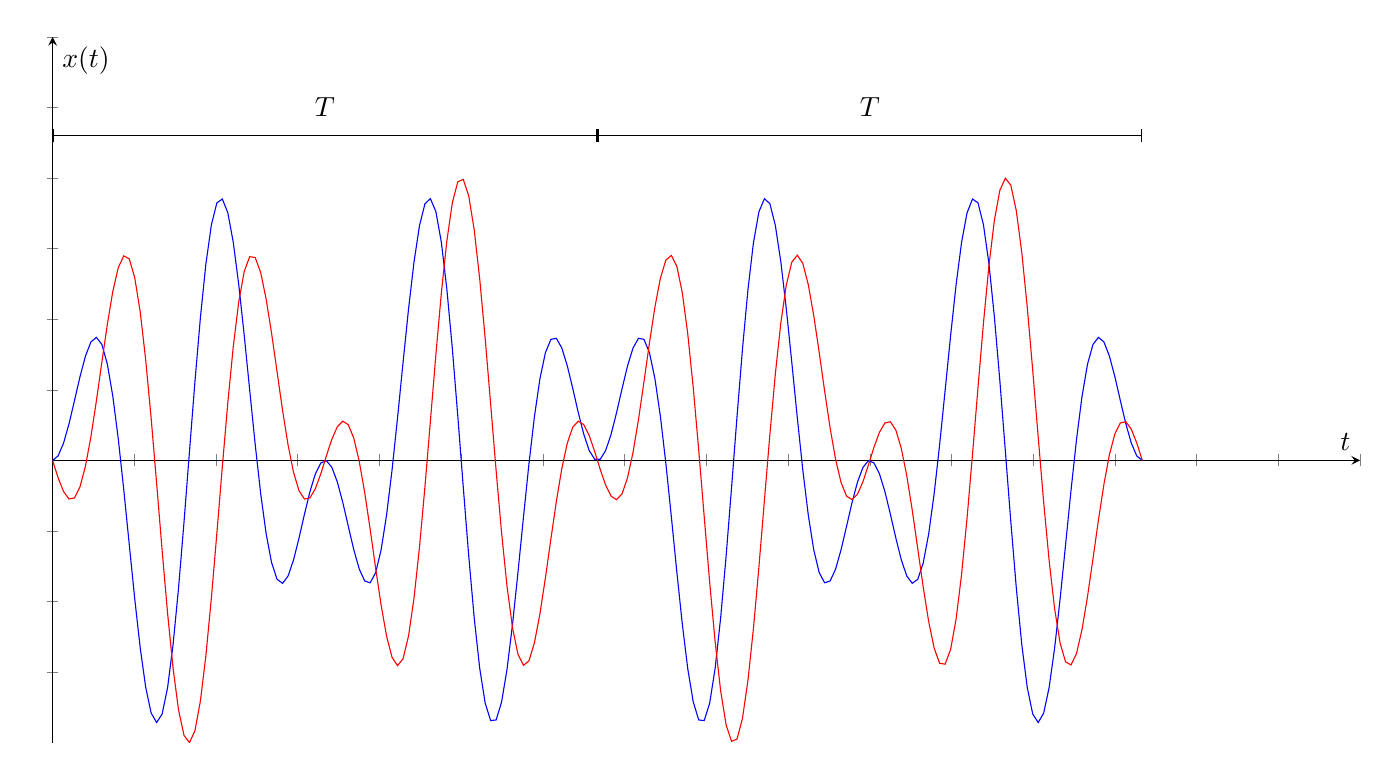
\begin{tikzpicture}
% \begin{pgfinterruptboundingbox}
\begin{axis}[width=1.5\textwidth, height=30em,
%	title={Discrete-time signal},
	axis x line=center,
	axis y line=middle,
        xmax=0.8,
        xlabel=$t$,
        xticklabels={,,},
        yticklabels={,,},
        ymax=3.0,
        ylabel=$x(t)$]

\addplot[domain=-0:0.666666667,samples=200,color=blue] {cos( deg(2*3.1415*9*x))-
                                              cos( deg(2*3.1415*15*x))};
\addplot[domain=-0:0.666666667,samples=200,color=red] {sin( deg(2*3.1415*9*x))-
                                                  sin( deg(2*3.1415*15*x))};

\node at (axis cs:0.16666667,2.5) {$\displaystyle{T}$};   
\addplot [dimen] plot coordinates {(0,2.3) (0.33333,2.3)};
\node at (axis cs:0.33333333+0.16666667,2.5) {$\displaystyle{T}$};   
\addplot [dimen] plot coordinates {(0.33333,2.3) (0.6666667,2.3)};

\end{axis}
%\end{pgfinterruptboundingbox}
%\draw[use as bounding box] ([xshift=0cm,yshift=0cm]current axis.south west) 
%    rectangle ([xshift=0cm,yshift=0cm]current axis.north east);
\end{tikzpicture}
\end{center}
\caption{Periodic function $e^{i 2\pi 9t} - e^{i 2\pi 15t}$. Blue denotes the real and red denotes the imaginary component of the signal.}
\label{fig:ex_periodic}
\end{marginfigure}

A consequence of Equation \ref{eq:integer_multiple} is that the ratios of all pairs of angular frequencies $\omega_k$ and $\omega_{\ell}$ 
in Equation \ref{eq:general_spectrum} need to be rational numbers. In other words, it must be possible to express them in the following form
\begin{equation}
\frac{\omega_k}{\omega_{\ell}} = \frac{n}{m} \in \mathbb{Q} \,\,
\end{equation}
in order for the signal to be periodic. Here $n$ and $m$ are arbitrary integers and $k$ and $\ell$ are all unique combinations of the frequency indices. 
If the ratio of two real numbers $\omega_1,\omega_2\in\mathbb{R}$ is a rational number $\omega_1/\omega_2 \in \mathbb{Q}$, the numbers $\omega_1$ and 
$\omega_2$ are called \emph{\index{commensurable}{commensurable}.} All angular frequencies for a Fourier series need to be commensurable relative to one another in order for the signal to be periodic.

How does one determine the fundamental frequency $\omega$? It is possible to apply \emph{\index{Euclid's algorithm}{Euclid's algorithm}}\footnote{Note that this is sometimes referred to as the \emph{greatest common divisor}, but this is only defined for
integers.} $\omega$ for the set of frequencies $\omega_k$. This algorithm will only produce a result in a finite number of steps if the set of numbers $\{\omega_k\}$ are commensurable, so it cannot be easily used as a test of periodicity.

\newthought{Here is an example}. Let us assume that a signal is defined as 
\begin{equation}
x(t) = c_1 e^{i \omega_1 t} + c_2 e^{i \omega_2 t} = e^{i 2\pi 9t}
- e^{i 2\pi 15t} \,\,.
\end{equation}
Is this signal periodic? If so, what is its fundamental frequency $\omega$ and fundamental period $T$?

In order for this signal to be periodic, $\omega_1$ and $\omega_2$ must be commensurable. In other words, $\omega_1/\omega_2 \in \mathbb{Q}$. This is the case, as it is clear that $\omega_1/\omega_2 = 3/5$ is a rational number.

This signal has two unique angular frequencies: $\omega_1 = 2\pi 9$ and $\omega_2 = 2\pi 15$. Let's use Euclid's algorithm\sidenote{The general principle behind the algorithm is that if $\omega_1 = \omega \ell_1$ and $\omega_2=\omega \ell_2$ with $\ell_1$ and $\ell_2$ integers, then $\omega_1 - \omega_2 = \omega(\ell_1-\ell_2)$ is still divisible with $\omega$.} on these two numbers to determine the fundamental angular frequency $\omega$. We start with the two numbers: $(2\pi 9, 2\pi15)$. We then subtract the smallest number from the largest number $2\pi 15 - 2\pi 9 = 2\pi 6$ and replace the larger number with the remainder: $(2\pi 9, 2\pi 6)$. We repeat this process until both numbers are the same. All of the iterations are shown below:
\begin{align*}
(2\pi 15, 2\pi 9) &\\
(2\pi 15-2\pi 9, 2\pi 9) &= (2\pi 6, 2\pi 9) \\
(2\pi 6, 2\pi 9-2\pi 6) &= (2\pi 6, 2\pi 3) \\
(2\pi 6-2\pi 3, 2\pi 3) &= (2\pi 3, 2\pi 3).
\end{align*}
And we thus find that the fundamental frequency is $\omega=2\pi 3$ and, using Equation \ref{eq:fundamental_period}, we find that $T = 1/3$.

\begin{marginfigure}[1cm]
\begin{center}
  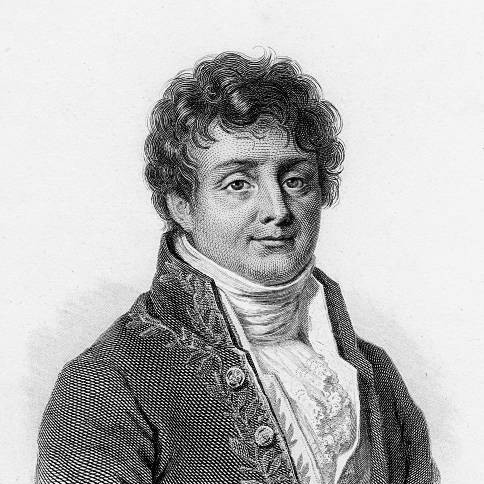
\includegraphics[width=\textwidth]{ch01/figures/fourier_head.jpg}
\end{center}
\caption{Jean-Baptiste Joseph Fourier}
\label{fig:joe_fourier2}
\end{marginfigure}

\newthought{The Fourier series is a spectral representation of a periodic function} and is defined as 
\begin{equation}
\boxed{
x_N(t) = \sum_{k=-N}^{N} c_k e^{i \frac{2\pi}{T} k t}
\label{eq:synthesis_eq}
} \,\,.
\end{equation}
The fundamental period of a periodic signal is related to the fundamental angular frequency as follows: $T=2\pi/\omega$. 
We can turn this around and express the fundamental angular frequency as a function of the fundamental period $\omega=2\pi/T$, as we have done above.


%\footnote{The Fourier series converges to a wide range of integrable periodic functions when $N\rightarrow \infty$. However, it is out of the scope of these lecture notes to discuss when the series converges and when it doesn't.}

This Fourier series is named after Jean-Baptiste Joseph Fourier (1768–1830). He introduced this representation for the purpose of solving the heat equation with periodic boundary conditions using a series of sinusoidal characteristic solutions. Perhaps the most revolutionary outcome of his study was that a wide range of functions can be represented as a sum of elementary sinusoidal functions.

Given a set of Fourier series coefficients $c_k$, we can synthesize a signal $x_N(t)$. This procedure is called \emph{\index{synthesis}{synthesis}}. 
This formula shown in Equation \ref{eq:synthesis_eq} is also called the Fourier series synthesis equation.

The inverse operation, determining coefficients $c_k \in \mathbb{C}$ from a certain periodic signal $x(t)$, is called \emph{\index{analysis}{analysis}}. 
We'll slowly work our way to this formula.

We will not study the convergence of the Fourier series, which means investigating if $\lim_{N\rightarrow \infty} x_N(t) = x(t)$. This is outside the scope of this course.

\newthought{In order to find the analysis formula, we'll first need to introduce the concept of basis functions and an inner product}. 
A Fourier series basis function is defined as $\psi_k(t)=e^{i\frac{2\pi}{T} k t}$. We can use this to write the Fourier series in the following form:
\begin{equation}
x_N(t) = \sum_{k=-N}^{N} c_k e^{i \frac{2\pi}{T} k t} = \sum_{k=-N}^{N} c_k \psi_k(t) \,\,.
\end{equation}
The terms $\psi_k(t)$ can be seen as a set of orthogonal basis functions for a periodic function with a period $T$. What does it mean that basis functions $\psi_k(t)$ are orthogonal? We'll first need to define an inner product.


%The set of basis function
%$\{\psi_k(t)\}_{k=-\infty}^{\infty}$ forms a vector space.\footnote{In mathematics, we would talk about a Hilbert space
%in this context. We have tried to avoid going into too much detail about
%this topic here.}


%\sidenote{If you are familiar with what a Hilbert space is, then you'll recognize this. Don't worry if you've never even heard of a Hilbert space though.}

For periodic functions $a(t)$ and $b(t)$ with period $T$, an inner product is defined as:
\begin{equation}
\langle a(t), b(t) \rangle = \int_{t_0}^{t_0+T} a(t) b^*(t) dt = \int_T a(t) b^*(t) dt \,\,,
\label{eq:inner_product_def}
\end{equation}
where $t_0$ is an arbitrary value of time, and $T$ is the fundamental period of the signal. 
Because of the periodicity of the signals, we can evaluate the integral at any offset $t_0$ we wish to. 
The right-hand side is just an alternative way to denote the equation in the middle, i.e., that we integrate over one period of the periodic function. 

When taking the inner product between two basis functions, we obtain:
\begin{align}
\langle \psi_\ell(t), \psi_k(t) \rangle &= \int_T \psi_\ell(t) \psi_k^*(t) dt\\
&= \int_T e^{i\frac{2\pi}{T}(\ell-k) t} dt \,\,.
\end{align}
Let's break this down into two cases. First let's look at $\ell=k$. We know that $e^{i(2\pi t/T)(\ell-\ell)}=e^{i \cdot 0} = 1$. It is easy to see that:
\begin{align}
\langle \psi_\ell(t), \psi_\ell(t) \rangle &= \int_{0}^T dt \\
&= T \,\,.
\end{align}
I've arbitrarily chosen to use $t_0=0$ when evaluating the integral (see the definition of the inner product in Equation \ref{eq:inner_product_def}). I would have obtained the same result with any value of $t_0$. 

Let's look at the other case where $\ell \ne k$. This means that the frequencies of the complex sinusoidal signals are different. We know that $\ell - k$ is a non-zero integer. Evaluating the inner product in this case gives us:
\begin{align}
\langle \psi_\ell(t), \psi_k(t) \rangle &= \int_0^T  e^{i\frac{2\pi}{T}t(\ell-k)} dt\\
&= \left.\frac{T}{2\pi i (\ell-k)} e^{i\frac{2\pi}{T}t(\ell-k)} \right\vert_{t=0}^{T} \\
&= \frac{T}{2\pi i (\ell-k)}\left( e^{i\frac{2\pi}{T}T(\ell-k)} - e^{i\frac{2\pi}{T}0(\ell-k)} \right)\\
&= \frac{T}{2\pi i (\ell-k)}( 1 - 1 ) \\
&= 0 \,\,.
\end{align}
We can combine these two results conveniently as:
\begin{align}
\langle \psi_\ell(t), \psi_k(t) \rangle = T\delta_{\ell,k} \,\,.
\end{align}
The integral thus evaluates to $T$ when $\ell=k$ and zero otherwise. We have used the Kronecker delta function $\delta_{k,\ell}$ for convenience. It is defined as:
\begin{equation}
\delta_{k,\ell} = \left\{
  \begin{array}{rcr}
    1 & \mathrm{when} & \ell=k \\
    0 & \mathrm{when} & \ell \ne k \\
  \end{array}\right.\,\,.
%\right\} 
\end{equation}
We now have what we need to introduce the analysis formula.

\newthought{The Fourier series analysis formula is defined as}:
\begin{equation}
\boxed{
c_k = \frac{1}{T}\langle x(t), \psi_k(t) \rangle = \frac{1}{T}\int_T x(t) \psi_k^*(t) dt = \frac{1}{T}\int_T x(t) e^{-i \frac{2\pi}{T} k t} dt
} \,\,.
\end{equation}
This formula can be used to determine what the Fourier series coefficients are for a periodic function $x(t)$. The proof for the analysis formula relies on the orthogonality of basis functions. We'll make the assumption that there exists a Fourier series representation for the signal $x(t)$ in the form of an infinite sum and that this sum converges uniformly\sidenote{The mathematician A.N. Kolmogorov pointed out in his 1923 paper several examples of functions for which the Fourier series diverges. The topic Fourier series convergence is beyond the scope of this course. \cite{kolmogoroff1923serie}}:
\begin{equation}
x(t) = \sum_{\ell=-\infty}^{\infty} c_{\ell} e^{i\frac{2\pi}{T}\ell t} \,\,.
\end{equation}
If this is the case, then the inner product, i.e., the analysis
equation, has the following result:
\begin{align}
\frac{1}{T}\langle x(t), \psi_k(t) \rangle &= \frac{1}{T}\int_T \left(\sum_{\ell=-\infty}^{\infty} c_\ell e^{i\frac{2\pi}{T}\ell t}\right) e^{-i\frac{2\pi}{T}k t}dt\\
&=\frac{1}{T}\sum_{\ell=-\infty}^{\infty} \int_T c_{\ell} e^{i\frac{2\pi}{T}\ell t} e^{-i\frac{2\pi}{T}kt}dt \\
  &= \frac{1}{T}\sum_{\ell=-\infty}^{\infty}c_{\ell} \int_T e^{i\frac{2\pi}{T}(\ell-k)t}dt \\
  &= \frac{1}{T}\sum_{\ell=-\infty}^{\infty}c_{\ell} T \delta_{\ell,k}\\
  &= c_k \,\,.
\end{align}
This proves that we can go back and forth between the Fourier synthesis and analysis formula, as long as there exists a Fourier series representation that converges uniformly for the periodic signal $x(t)$.

\newthought{We now have the synthesis and analysis formulas for a Fourier series}. The synthesis formula allows us to obtain the time domain representation of a periodic signal using Fourier coefficients:
\begin{equation}
\boxed{
x_N(t) = \sum_{k=-N}^{N} c_k e^{i \frac{2\pi}{T}kt}
} \,\,.
\end{equation}
The inverse operation, i.e., obtaining the Fourier coefficients $c_k$ from a periodic function $x(t)$, is as follows:
\begin{equation}
\boxed{
c_k = \frac{1}{T} \int_T x(t) e^{-i \frac{2\pi}{T}kt} dt
} \,\,.
\end{equation}

\newthought{What about real-valued signals?} We can use Euler's formula to look at the real part of the Fourier series synthesis formula. I'll assume again that $x(t)$ is a periodic function that can be represented using an infinite sum of complex sinusoidal signals:
\begin{equation}
x(t) = \sum_{\ell = -\infty}^{\infty} c_{\ell} e^{i\frac{2\pi}{T}\ell t}.
\end{equation}
The real part of the signal $x(t)$ is:
\begin{align}
\mathrm{Re}\{x(t)\} &= \frac{1}{2} (x(t) + x^*(t)) \\
&= \frac{1}{2}\sum_{\ell=-\infty}^{\infty} c_{\ell} e^{i\frac{2\pi}{T}\ell t} + \frac{1}{2}\sum_{\ell=-\infty}^{\infty} c^*_{\ell} e^{-i\frac{2\pi}{T}\ell t} \\
&= \frac{1}{2}(c_0 + c_0^*) + \frac{1}{2}\sum_{\ell=1}^{\infty}[ (c_{\ell} + c^*_{-\ell}) e^{i\frac{2\pi}{T}\ell t} + (c^*_{\ell} + c_{-\ell}) e^{-i\frac{2\pi}{T}\ell t}]\\
&= A_0 + \sum_{\ell=1}^{\infty} A_\ell \cos\left(\frac{2\pi}{T}\ell t+\phi_\ell\right) \,\,.
\label{eq:real_fourier_series}
\end{align}
For the last part, I've introduced new variables: $A_0= \frac{1}{2}(c_0 + c_0^*) \in \mathbb{R}$, $A_\ell = |c_{\ell} +c^*_{-\ell}|\in \mathbb{R}_{\ge 0}$ and $\phi_\ell = \angle (c_{\ell} + c^*_{-\ell}) \in \mathbb{R}$. 

When analyzing Fourier series coefficients for a real-valued function, you will find that they come in conjugate symmetric pairs, 
which will allow you to write the Fourier series synthesis equation in the form shown on the last line of Equation \ref{eq:real_fourier_series}. 
Also, the Fourier series synthesis equation is sometimes introduced in this form in older texts.

\newthought{The zero frequency or the direct current (DC) frequency component $c_0$} often has a special meaning. In the case of real-valued signals, 
this is the only frequency component that does not have a positive and negative frequency conjugate symmetric pairing. The DC component also has the meaning that it is the mean value of the signal:
\begin{equation}
c_0 = \frac{1}{T} \int_{T} x(t) dt \,\,.
\end{equation}

\newthought{A partial sum Fourier series can be used to approximate a periodic signal}. This is especially useful, if one knows that the signal is band-limited, 
and one knows \emph{a priori} that higher order terms (high frequency components) are not present in the signal, or they have such low magnitudes that they are not significant. 

A partial sum synthesis formula only uses a subset of the Fourier coefficients:
\begin{equation}
x_S(t) = \sum_{k \in S} c_k e^{i 2\pi kt/T} \,\,,
\end{equation}
where $S$ is a set of Fourier series coefficient indices.

\begin{marginfigure}
\begin{center}
\begin{tikzpicture}
\pgfmathdeclarefunction{p}{1}{%
  \pgfmathparse{(and(mod(#1,2)>0, mod(#1,2)<1))}%
} \begin{axis}[
width=7cm,
axis lines = center,
ymax=1.5,
ymin=0,
xmax=3.5,
xmin=-3.5,
legend pos=outer north east,
yticklabels={,,},
xticklabels={,,},
xlabel={$t$},
ylabel={$x(t)$}
]
    
    \addplot+[ycomb,color=blue,mark=triangle*,mark options={blue}] plot coordinates {
    (-3,1)
    (-2,1)
    (-1,1)
    (-0,1)
    (1,1)
    (2,1)
    (3,1)
};

\node at (axis cs:1.5,1.15) {$\displaystyle{T}$};   
\addplot [dimen] plot coordinates {(1,1.1) (2,1.1)};

\end{axis}
\end{tikzpicture}
\end{center}
\caption{The Dirac comb signal, an infinitely long train of unit impulses spaced apart by $T$. The Dirac comb is a periodic function with a fundamental period $T$. 
The Dirac comb is used to model sampling values of a continuous-time signal spaced evenly apart to provide an idealized model for discretizing a continuous-time signal.}
\label{fig:dirac_comb_plot2}
\end{marginfigure}

A partial sum approximation of this type is often used in audio, image, and video compression, which rely on storing only a small subset of Fourier series coefficients, which typically have the largest magnitudes, leaving out the frequency components with small magnitudes.

\newthought{Example: Let's represent the so called Dirac comb using a Fourier series}.
The Dirac comb is a signal that consists of a train of unit impulse functions spaced $T$ apart from one another. It is defined as:
\begin{equation}
x(t) = \sum_{k=-\infty}^{\infty} \delta(t - k T) \,\,.
\end{equation}
This signal is shown in Figure \ref{fig:dirac_comb_plot2}. We'll encounter this signal when introducing the model for discretizing a continuous-time signal. 

The fundamental period for this signal is $T$. Therefore, one would expect that we can form a Fourier series representation of this signal. What are the values of the coefficients $c_k$? Let's find out using the analysis formula.

We'll evaluate the analysis integral formula from $t=-T/2$ to $t=T/2$, as this is convenient in the case of this signal. The analysis formula evaluates to:
\begin{align}
c_k &= \langle x(t),\psi_k(t) \rangle = \frac{1}{T} \int_{-T/2}^{T/2} \delta(t) e^{-i\frac{2\pi}{T}kt} dt \\
&= \frac{1}{T}\label{eq:dirac_comb_coeff} \,\,.
\end{align}
The signal can thus be represented as the following Fourier series:
\begin{equation}
x_N(t) = \frac{1}{T}\sum_{k=-N}^{N} e^{i\frac{2\pi}{T}kt} \,\,. 
\end{equation}
Take a look at Figure \ref{fig:fs_fig0}. This is an approximation of the Dirac comb $x_7(t)$ using 15 frequency components. 
I hope it is not too difficult for you to convince yourself that as we increase the value of $N$, the spikes will become sharper and sharper.

\begin{marginfigure}[-8cm]
\begin{center}
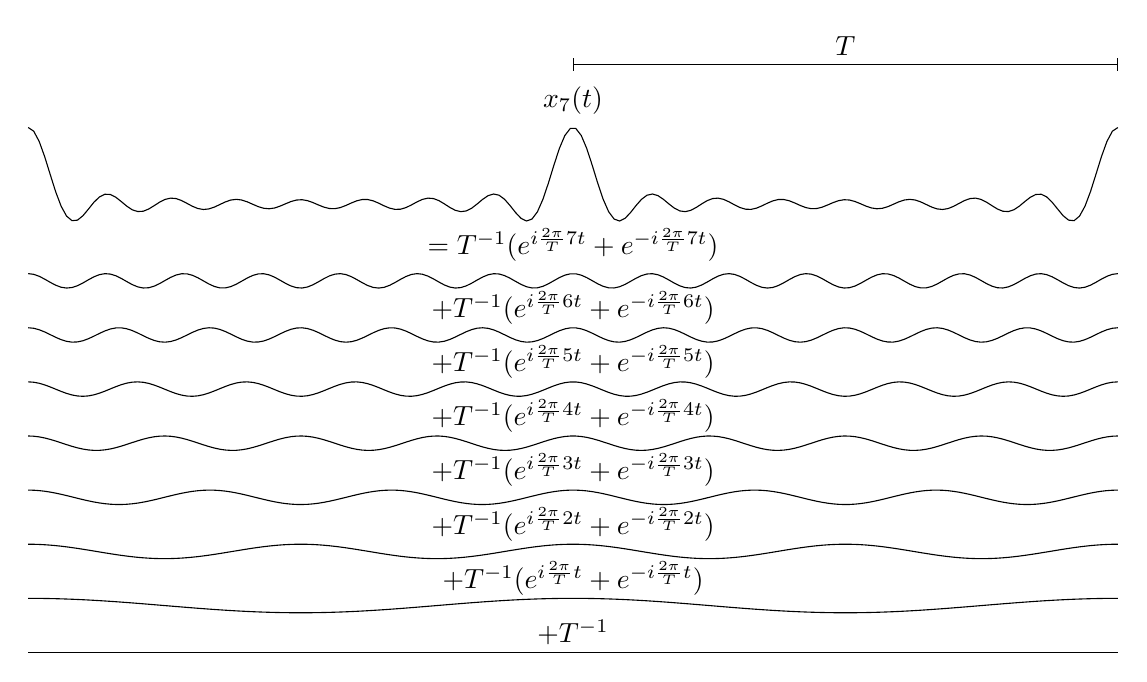
\begin{tikzpicture}
% \begin{pgfinterruptboundingbox}
\begin{axis}[width=1.5\textwidth, height=30em,
%	title={Discrete-time signal},
	axis x line=none,
	axis y line=none
]
\addplot[domain=-100:100,samples=200] {27+
                                       cos( deg(2*3.1415*0.01*x))+
                                       cos( deg(2*3.1415*0.01*2*x) )+
                                       cos( deg(2*3.1415*0.01*3*x) )+
                                       cos( deg(2*3.1415*0.01*4*x) )+
                                       cos( deg(2*3.1415*0.01*5*x) )+
                                       cos( deg(2*3.1415*0.01*6*x) )+
                                       cos( deg(2*3.1415*0.01*7*x) )+
                                       cos( deg(2*3.1415*0.01*8*x) ) };

\node at (axis cs:50.0,44) {$\displaystyle{T}$};   
\addplot [dimen] plot coordinates {(0,42) (100,42)};

\node at (axis cs:0,38) {$x_{7}(t)$};

\node at (axis cs:0,22) {$= T^{-1} (e^{i\frac{2\pi }{T}7t} + e^{-i\frac{2\pi }{T}7t})$};
\node at (axis cs:0,15) {$+ T^{-1} (e^{i\frac{2\pi }{T}6t} + e^{-i\frac{2\pi }{T}6t})$};
\node at (axis cs:0,9) {$+ T^{-1}(e^{i\frac{2\pi }{T}5t} + e^{-i\frac{2\pi }{T}5t})$};
\node at (axis cs:0,3) {$+ T^{-1}(e^{i\frac{2\pi }{T}4t} + e^{-i\frac{2\pi }{T}4t})$};
\node at (axis cs:0,-3) {$+ T^{-1}(e^{i\frac{2\pi }{T}3t} + e^{-i\frac{2\pi }{T}3t})$};
\node at (axis cs:0,-9) {$+ T^{-1}(e^{i\frac{2\pi }{T}2t} + e^{-i\frac{2\pi }{T}2t})$};
\node at (axis cs:0,-15) {$+ T^{-1}(e^{i\frac{2\pi }{T}t} + e^{-i\frac{2\pi }{T}t})$};
\node at (axis cs:0,-21) {$+ T^{-1}$};

\addplot[domain=-100:100,samples=200] {-24+0.8*cos( deg(2*3.1415*0.0*x) ) };
\addplot[domain=-100:100,samples=200] {-18+0.8*cos( deg(2*3.1415*0.01*x) ) };
\addplot[domain=-100:100,samples=200] {-12+0.8*cos( deg(2*3.1415*0.01*2*x) ) };
\addplot[domain=-100:100,samples=200] {-6+0.8*cos( deg(2*3.1415*0.01*3*x) ) };
\addplot[domain=-100:100,samples=200] {0+0.8*cos( deg(2*3.1415*0.01*4*x) ) };
\addplot[domain=-100:100,samples=200] {6+0.8*cos( deg(2*3.1415*0.01*5*x) ) };
\addplot[domain=-100:100,samples=200] {12+0.8*cos( deg(2*3.1415*0.01*6*x) ) };
\addplot[domain=-100:100,samples=200] {18+0.8*cos( deg(2*3.1415*0.01*7*x) ) };

\end{axis}
%\end{pgfinterruptboundingbox}
%\draw[use as bounding box] ([xshift=0cm,yshift=0cm]current axis.south west) 
%    rectangle ([xshift=0cm,yshift=0cm]current axis.north east);
\end{tikzpicture}
\end{center}
\caption{A Fourier series representation $x_{7}(t)=\frac{1}{T}\sum_{k=-7}^{7} e^{i\frac{2\pi}{T}k t}$ of a Dirac comb signal $x(t)=\sum_{k=-\infty}^{\infty}\delta(t-k T)$
with a period $T$. Two periods of the signal are shown. The Fourier series representation of the signal is made using seven sinusoidal signals.}
\label{fig:fs_fig0}
\end{marginfigure}

You may also be able to convince yourself that this signal is real-valued, by investigating the pairing of positive and negative frequency terms:
\begin{align}
x_N(t) &= \frac{1}{T}\sum_{k=-N}^{N} e^{i\frac{2\pi}{T}kt}\\
&= \frac{1}{T} + \frac{1}{T} \sum_{k=1}^{N} (e^{i\frac{2\pi}{T}kt}+e^{-i\frac{2\pi}{T}kt})\\
&= \frac{1}{T} + \frac{2}{T} \sum_{k=1}^{N} \cos\left( \frac{2\pi}{T}kt \right ) \,\,.
\end{align}
This is how the positive and negative frequency terms are organized in Figure \ref{fig:fs_fig0}. For real-valued Fourier series representations, this sort of grouping of positive and negative frequency coefficients always occurs.


\newthought{Example: Fourier series representation for a square wave}. A square wave is a
classic example of a periodic function that can be evaluated using a Fourier series. This type of signal is often used, e.g., in the pulse width modulation scheme of adjusting mean power flowing through a circuit. 
This type of on-off pulsing scheme is also used in avalanche rescue beacons used to radiolocate victims buried under snow. The rectangular function is shown in Figure \ref{fig:square_wave_example}. 
A measurement of power emitted by an avalanche rescue beacon as a function of time is shown in Figure \ref{fig:avibeacon}.

\begin{marginfigure}
\begin{center}
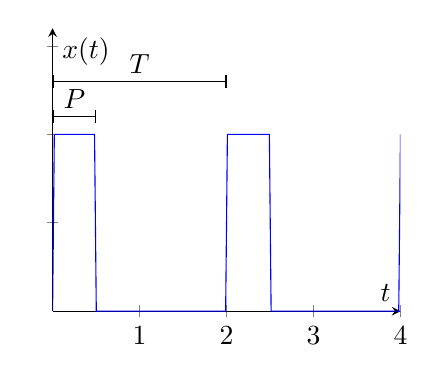
\begin{tikzpicture}
\pgfmathdeclarefunction{p}{1}{%
  \pgfmathparse{(and(mod(#1,2)<0.5,and(mod(#1,2)>0, mod(#1,2)<1)))}%
}
	\begin{axis}[
        width=6cm,
        domain=0:(4),
        samples=200,
        axis lines =center,
        ymax=1.6,
        yticklabels={,,},
        legend pos=outer north east ,xlabel={$t$},ylabel={$x(t)$}]
    \addplot[blue] {p(x)};

\node at (axis cs:0.25,1.2) {$\displaystyle{P}$};   
\addplot [dimen] plot coordinates {(0,1.1) (0.5,1.1)};

\node at (axis cs:1,1.4) {$\displaystyle{T}$};   
\addplot [dimen] plot coordinates {(0,1.3) (2,1.3)};


%    \legend{$\mathrm{Re}(e^{j2t})$,$\mathrm{Im}(e^{j2t})$}
    \end{axis}
\end{tikzpicture}
\end{center}
\caption{A classic example of a commonly encountered periodic function, the square wave signal. This type of signal is encountered, e.g., with pulse width modulation in electrical engineering.}
\label{fig:square_wave_example}
\end{marginfigure}


\begin{marginfigure}
\begin{center}
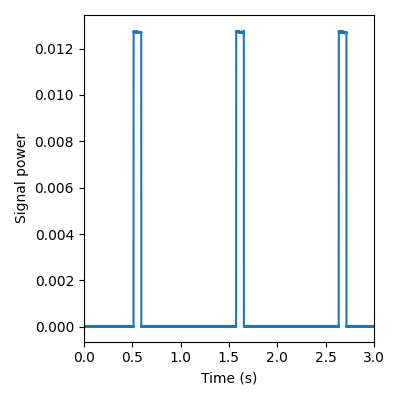
\includegraphics[width=\textwidth]{ch07/figures/avibeacon.png}
\end{center}
\caption{A measurement of power as a function of time transmitted by an avalanche rescue locator beacon. Approximately a 0.1 second pulse is emitted every second.}
\label{fig:avibeacon}
\end{marginfigure}

Consider a general square wave signal with period $T$, pulse length $P$ and amplitude $1$. Between $0\le t < T$, this signal is mathematically described with:
\begin{equation}
x(t) = \left\{ \begin{array}{ccl}
1 & \mathrm{when} & 0 \le t < P \\
0 & \mathrm{otherwise} & 
\end{array}
\right. \,\,.
\end{equation}
By analytically evaluating the Fourier series analysis integral one has:
\begin{equation}
c_k = \frac{1}{T}\int_0^T x(t) e^{-i 2\pi k t/T} dt \,\,,
\end{equation}
we can obtain an equation for coefficients $c_k$. In the case of $k=0$, the integral evaluates to:
\begin{align}
c_0 & = \frac{1}{T}\int_0^{T} x(t) e^{i\cdot 0}dt\\
    & = \frac{1}{T}\int_0^{P}  dt \\
    & = \frac{P}{T} \,\,.\label{eq:pulsecoeff0}
\end{align}
For other values of $k\ne 0$:
\begin{align}
c_k & = \frac{1}{T}\int_0^{T} x(t) e^{-i\frac{2\pi}{T} t k}dt\\
 & =  \frac{1}{T}\int_0^{P}  e^{-i\frac{2\pi}{T} t k}dt \\
 & = \left.-\frac{1 }{2i \pi k}e^{-i\frac{2\pi}{T}  t k}\right\vert_{t=0}^{P} \\
 & = -\frac{1}{2i\pi k}\left(e^{-i\frac{2\pi}{T}  k P} - 1\right)\\
 & = \frac{1}{2i\pi k}e^{-i\frac{\pi}{T}  k P}\left(e^{i \frac{\pi}{T} kP} - e^{-i \frac{\pi}{T} kP} \right)\\
& =  \frac{1}{\pi k}e^{-i\frac{\pi}{T}  k P}\sin\left(\frac{\pi}{T} kP\right) \,\,.\label{eq:pulsecoeff1}
\end{align}
We have used: the inverse Euler's formula for the $\sin(\cdot)$ signal, the fact that $e^{-i\frac{\pi}{T} k P}e^{i\frac{\pi}{T} k P}=1$, and that $\sin(-\theta)=-\sin(\theta)$. 

\begin{marginfigure}
\begin{center}
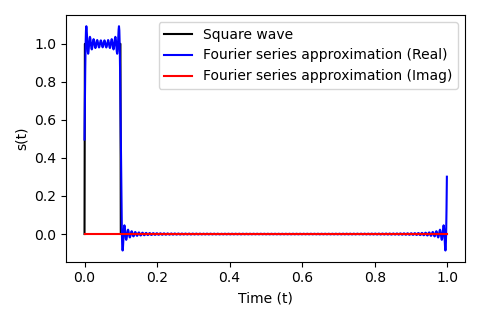
\includegraphics[width=\textwidth]{code/009_square_wave/square_wave.png}
\end{center}
\caption{Fourier series approximation of a square wave evaluated with the Python script \texttt{009\_square\_wave/square\_wave.py}.}
\label{fig:square_wave_python}
\end{marginfigure}

Now we can evaluate the synthesis formula to form a Fourier series approximation of this function:
\begin{align}
x_N(t) & = c_0 + \sum_{k=1}^{N} c_k e^{i\frac{2\pi}{T}kt} + c_{-k} e^{-i\frac{2\pi}{T}kt} \\
   & = \frac{P}{T} + \sum_{k=1}^{N} \frac{\sin\left(\frac{\pi}{T} kP\right)}{\pi k}  \left(e^{-i\frac{\pi}{T}kP}e^{i\frac{2\pi}{T}kt} + e^{i\frac{\pi}{T}kP}e^{-i\frac{2\pi}{T}kt}\right) \\
   & = \frac{P}{T} + \sum_{k=1}^{N} \frac{2\sin\left(\frac{\pi}{T} kP\right)}{\pi k} \cos\left( \frac{2\pi}{T}kt-\frac{\pi}{T}kP\right) \,\,.
\end{align}
Let's see what this function looks like. I've written a little Python
program to visualize the Fourier series approximation of this
function. The Python code is found in
Listing \ref{lst:fourier_square_code}. The output of this program is shown in Figure \ref{fig:square_wave_python}.

\lstinputlisting[language=Python,caption={\texttt{009\_square\_wave/square\_wave.py}},label=lst:fourier_square_code]{code/009_square_wave/square_wave.py}

\if 0
\begin{center}
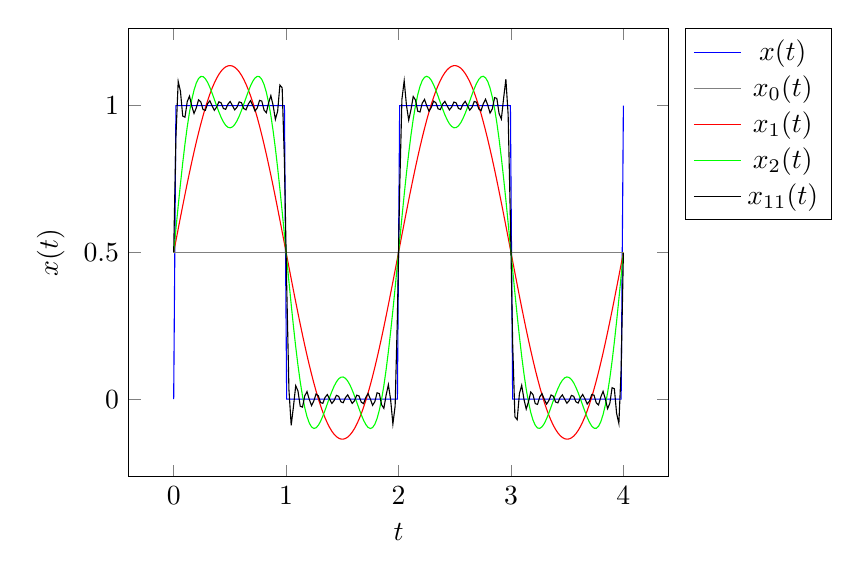
\begin{tikzpicture}
\pgfmathdeclarefunction{p}{1}{%
  \pgfmathparse{(and(mod(#1,2)>0, mod(#1,2)<1))}%
}
	\begin{axis}[domain=0:(4),samples=200, legend pos=outer north east ,xlabel={$t$},ylabel={$x(t)$}]
    \addplot[blue] {p(x)};
    \addplot[gray] {0.5}; % k=0
    \addplot[red] {0.5 + (2.0/3.1415)*cos(deg(3.1415*x - 1.571))}; % k=1
    \addplot[green] {0.5 + (2.0/3.1415)*cos(deg(3.1415*x - 1.571)) + (2.0/(3.1415*3))*cos(deg(3.1415*3*x - 1.571))}; % k=2
  %  \addplot[orange] {0.5 + (2.0/3.1415)*cos(deg(3.1415*x - 1.571)) + (2.0/(3.1415*3))*cos(deg(3.1415*3*x - 1.571)) + (2.0/(3.1415*5))*cos(deg(3.1415*5*x - 1.571))}; % k=5
    \addplot[black] {0.5 + (2.0/3.1415)*cos(deg(3.1415*x - 1.571))
                     + (2.0/(3.1415*3))*cos(deg(3.1415*3*x - 1.571)) 
                     + (2.0/(3.1415*5))*cos(deg(3.1415*5*x - 1.571))
                     + (2.0/(3.1415*7))*cos(deg(3.1415*7*x - 1.571))
                     + (2.0/(3.1415*9))*cos(deg(3.1415*9*x - 1.571))
                     + (2.0/(3.1415*11))*cos(deg(3.1415*11*x - 1.571))
                     + (2.0/(3.1415*13))*cos(deg(3.1415*13*x - 1.571))
                     + (2.0/(3.1415*15))*cos(deg(3.1415*15*x - 1.571))
                     + (2.0/(3.1415*17))*cos(deg(3.1415*17*x - 1.571))
                     + (2.0/(3.1415*19))*cos(deg(3.1415*19*x - 1.571))
                     + (2.0/(3.1415*21))*cos(deg(3.1415*21*x - 1.571))};
%%                     + (2.0/(3.1415*23))*cos(deg(3.1415*23*x - 1.571))
%                     + (2.0/(3.1415*25))*cos(deg(3.1415*25*x - 1.571))
%                     + (2.0/(3.1415*27))*cos(deg(3.1415*27*x - 1.571))
%                     + (2.0/(3.1415*29))*cos(deg(3.1415*29*x - 1.571))
%                     + (2.0/(3.1415*31))*cos(deg(3.1415*31*x - 1.571))
%                     + (2.0/(3.1415*33))*cos(deg(3.1415*33*x - 1.571))
%                     + (2.0/(3.1415*35))*cos(deg(3.1415*35*x - 1.571))
%                     + (2.0/(3.1415*37))*cos(deg(3.1415*37*x - 1.571)) 
%                     + (2.0/(3.1415*39))*cos(deg(3.1415*39*x - 1.571)) 
%                     + (2.0/(3.1415*41))*cos(deg(3.1415*41*x - 1.571)) 
%                     + (2.0/(3.1415*43))*cos(deg(3.1415*43*x - 1.571)) 
%                     + (2.0/(3.1415*45))*cos(deg(3.1415*45*x - 1.571)) 
%                     + (2.0/(3.1415*47))*cos(deg(3.1415*47*x - 1.571)) 
%                     + (2.0/(3.1415*49))*cos(deg(3.1415*49*x - 1.571)) 
%                     + (2.0/(3.1415*51))*cos(deg(3.1415*51*x - 1.571)) 
%                     + (2.0/(3.1415*53))*cos(deg(3.1415*53*x - 1.571)) 
%                     + (2.0/(3.1415*55))*cos(deg(3.1415*55*x - 1.571))};

    \legend{$x(t)$,$x_0(t)$,$x_1(t)$,$x_2(t)$,$x_{11}(t)$}
    \end{axis}
\end{tikzpicture}
\end{center}
\fi

\newthought{The time derivative operator $\frac{d}{dt}$ has a very simple form for a Fourier series representation of a signal}.

We know that a Fourier series is a sum of complex sinusoidal signals. We also know that it is easy to differentiate this signal:
\begin{equation}
\frac{d}{d t} c e^{i\omega t}=i\omega c e^{i\omega t}\,\,,
\end{equation}
where $c \in \mathbb{C}$ is a complex constant.

It is also relatively easy to see that the $n$th time derivative is:
\begin{equation}
\frac{d^n}{dt^n}ce^{i\omega t} = (i\omega)^n c e^{i\omega t} \,\,.
\end{equation}
Thus, if $x(t)$ has a Fourier series representation
\begin{equation}
x(t) = \sum_{k=-\infty}^{\infty} c_k e^{i\frac{2\pi}{T}kt}\,\,,
\end{equation}
then the $n$th time derivative has the following Fourier series representation:
\begin{align}
\frac{d^n}{dt^n} x(t) &= \sum_{k=-\infty}^{\infty} i^n \left(\frac{2\pi k}{T}\right)^n c_k e^{i\frac{2\pi}{T}kt}\\
&= \sum_{k=-\infty}^{\infty} c^{(n)}_k e^{i\frac{2\pi}{T}kt} \,\,.
\end{align}
It is still a Fourier series, but with each Fourier coefficient modified in the following way:
\begin{equation}
c_k^{(n)} := i^n \left(\frac{2\pi k}{T}\right)^n c_k \,\,.
\label{eq:moddiff}
\end{equation}

Differentiation can be seen as a filtering operation on the signal. A filter is something that modifies the amplitude and phase of the Fourier series coefficients in some way. 
For example, a low-pass filtering operation would reduce the amplitudes of high frequency coefficients relative to the amplitudes of the low frequency coefficients. 
After a low-pass filtering operation, the ratio of low frequency coefficient amplitudes to the high frequency coefficient amplitudes would be increased. A high pass filter on the other hand would do the opposite.

One thing to ask yourself is how does differentiation adjust the amplitude of each Fourier coefficient? When taking the $n$th time derivative, what happens to the complex amplitudes at low angular frequencies ($|2\pi k/T| < 1$)? What about high angular frequencies ($|2\pi k/T| > 1$)? Hint, inspect how the coefficients defined in Equation \ref{eq:moddiff} are scaled.

The answer is that the magnitude of the low frequency Fourier coefficients are attenuated, and high frequency ones are amplified. The DC component is completely removed as $2\pi k/T = 0$ for $k=0$. 
Differentiation can therefore be viewed as a \emph{high-pass filtering} operation.

\newthought{The time shift operation $x(t-\tau)$ applied to a Fourier series representation} is also pretty handy. 
Let's recall how a time shift affects a complex sinusoidal signal:
\begin{equation}
x(t) = c e^{i\omega t} \,\,.
\end{equation}
If we apply a delay by $\tau$ to this signal $y(t) = x(t-\tau)$, we obtain:
\begin{align}
y(t)  = c e^{i\omega (t-\tau)} =  e^{-i\omega \tau} c e^{i\omega t} = e^{-i\omega \tau} x(t) \,\,.
\end{align}
This means that a time delay by $\tau$ corresponds to a phase shift by $-\omega\tau$ for a complex sinusoidal signal. We can apply this to a Fourier series, which is a sum of complex sinusoidal signals.

If the Fourier series representation of a signal is:
\begin{equation}
x(t) = \sum_{k=-\infty}^{\infty} c_k e^{i\frac{2\pi}{T}kt} \,\,,
\end{equation}
then the Fourier series representation of a time shifted signal is:
\begin{align}
x(t-\tau) & = \sum_{k=-\infty}^{\infty} \left(c_k e^{-i \frac{2\pi \tau}{T} k}\right) e^{i\frac{2\pi}{T}kt}\label{eq:time_shift_phasor}\\
          &=  \sum_{k=-\infty}^{\infty} c'_k e^{i\frac{2\pi}{T}kt}
\end{align}
where $c'_k$ is rotated on the complex plane in the clockwise direction by an angle of $2\pi k\tau/T$ with respect to $c_k$.

This means that if you know the Fourier series representation of a signal, you can easily modify the complex amplitude $c_k$ of each Fourier coefficient to obtain the coefficients of the time shifted signal.

\newthought{What if a signal is not periodic, can we still form a spectral representation for a signal?} Yes, we can. This investigation leads to the \emph{\index{continuous-time Fourier transform}{continuous-time Fourier transform}}.

Let's derive the continuous-time Fourier transform from the Fourier series. Pretty much all we'll need to do is to study what happens when the fundamental period of the signal approaches infinity: $T\rightarrow \infty$.  We'll arrive with the result that introduces the Fourier transform, and the inverse Fourier transform, introducing, for the first time, this general spectral representation for continuous-time signals.

We start the derivation of the continuous-time Fourier transform with the definition of a Fourier series for a function with period $T$. We'll denote by $\Delta \omega$ the spacing between frequency components. The term $\Delta \omega$ also denotes the fundamental angular frequency of the periodic signal:
\begin{align}
x_{T}(t) &= \sum_{k=-\infty}^{\infty} c_k e^{ik\Delta \omega t}  \,\,.
\end{align}
We can now add the definition of $c_k$ corresponding to the $k$th Fourier series coefficient using the synthesis equation:
\begin{align}
x_{T}(t) &= \sum_{k=-\infty}^{\infty} \left[\frac{1}{T}\int_{-T/2}^{T/2} x_{T}(t) e^{-ik\Delta \omega t} dt\right]  e^{ik\Delta \omega t}  \,\,.
\end{align}
We then note that $1/T = \Delta \omega/2\pi$. This is the relationship between the fundamental period of the signal and the fundamental angular frequency that we discussed in the beginning of this chapter.

We now obtain:
\begin{align}
x_{T}(t) &= \frac{1}{2\pi}\sum_{k=-\infty}^{\infty} \left[\int_{-T/2}^{T/2} x_{T}(t) e^{-ik\Delta \omega t} dt\right]  e^{ik\Delta \omega t} \Delta \omega\\
&= \frac{1}{2\pi}\sum_{k=-\infty}^{\infty} \hat{x}_{T}(k\Delta\omega)  e^{ik\Delta \omega t} \Delta \omega \,\,.
\end{align}
In this form, the equation is a Riemann sum approximation of an integral of a continuous function $\hat{x}_{T}(\omega)e^{-i\omega t}$.
\begin{figure}
\begin{center}
        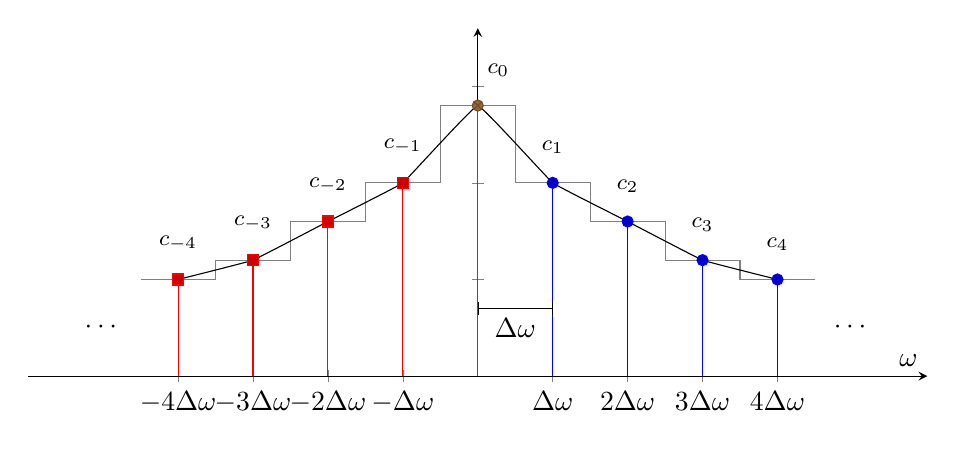
\begin{tikzpicture}
        \begin{axis}[width=13cm,height=6cm,ymin=-0,xmin=-3,ymax=1.8,xmax=3,  yticklabels={,,},
        xtick={-2,-1.5,-1,-0.5,0,0.5,1.0,1.5,2},
        xticklabels={$-4\Delta \omega$,$-3\Delta \omega$,$-2\Delta \omega$,$-\Delta \omega$,$0$,$\Delta \omega$,$2\Delta \omega$,$3\Delta \omega$,$4\Delta \omega$},
    xlabel=$\omega$, axis lines = center]
    
   \addplot+[ycomb] plot coordinates {(0.5,1) (1.0,0.8) (1.5,0.6) (2,0.5)};
    \addplot+[ycomb] plot coordinates {(-0.5,1) (-1.0,0.8) (-1.5,0.6) (-2,0.5)};
   \addplot+[ycomb] plot coordinates {(0.0, 1.4)};
    \node at (axis cs:-2.5,0.25) {$\cdots$};   
    \node at (axis cs:2.5,0.25) {$\cdots$};   
    \node at (axis cs:0.25,0.25) {$\Delta \omega$};   
    
       
%    \addplot [dimen] plot coordinates {(0.0,0.35) (0.5,0.35)};
%    \addplot  plot coordinates {(0.0,0.35) (0.5,0.35)};
       \addplot[dimen]  plot coordinates {(0.0,0.35) (0.5,0.35)};    
          \addplot[mark=none,color=gray] plot coordinates {(-2.25,0.5) (-1.75,0.5) (-1.75,0.6) (-1.25,0.6) (-1.25,0.8) (-.75,0.8) (-.75,1) (-.25,1) (-.25,1.4) (.25,1.4) (.25,1) (.75,1) (.75,0.8) (1.25,0.8) (1.25,0.6) (1.75,0.6) (1.75,0.5) (2.25,0.5)} ;

            \addplot[mark=none,color=black] plot [smooth,tension=0.1] coordinates {(-2.,0.5) (-1.5,0.6) (-1,0.8) (-.5,1) (0,1.4) (.5,1.) (1,0.8) (1.5,0.6) (2,0.5) } ;

    \node at (axis cs:0.0,1.5) [above right, font={\footnotesize}]{$c_0$};
    \node at (axis cs:0.5,1.1) [above, font={\footnotesize}]{$c_1$};
    \node at (axis cs:1.0,0.9) [above, font={\footnotesize}]{$c_2$};
    \node at (axis cs:1.5,0.7) [above, font={\footnotesize}]{$c_3$};
    \node at (axis cs:2.0,0.6) [above, font={\footnotesize}]{$c_4$};

    \node at (axis cs:-0.5,1.1) [above, font={\footnotesize}]{$c_{-1}$};
    \node at (axis cs:-1.0,0.9) [above, font={\footnotesize}]{$c_{-2}$};
    \node at (axis cs:-1.5,0.7) [above, font={\footnotesize}]{$c_{-3}$};
    \node at (axis cs:-2.0,0.6) [above, font={\footnotesize}]{$c_{-4}$};
\end{axis}
        \end{tikzpicture}
\end{center}
\caption{A depiction of how the Fourier series can be seen as a Riemann sum approximation of an integral of a continuous function.}
\end{figure}

We now inspect the case where $T\rightarrow \infty$. When the period of the function $x_{T}(t)$ approaches infinity, 
we drop the subscript $T$ in the notation and denote it with $x(t)$. The Riemann sum then approaches the following integral equation ($\Delta\omega \rightarrow d\omega$, $k\Delta\omega \rightarrow \omega$):
\begin{align}
\lim_{T\rightarrow \infty} x_{T}(t)  &= \lim_{T\rightarrow \infty}\frac{1}{2\pi} \sum_{k=-\infty}^{\infty} \hat{x}_{T}(k\Delta \omega) e^{ik\Delta \omega t}\Delta\omega \\
&=\frac{1}{2\pi}\int_{-\infty}^{\infty} \left[\int_{-\infty}^{\infty} x(t) e^{-i\omega t} dt\right] e^{i\omega t}d\omega\\
&= \frac{1}{2\pi} \int_{-\infty}^{\infty} \hat{x}(\omega) e^{i\omega t}d\omega\\
&= x(t) \,\,.
\end{align}
This integral is known as the inverse Fourier transform. It allows us to go from a continuous function $\hat{x}(\omega)$, 
which is the continuous spectral representation of the signal, to the time domain signal $x(t)$.

The innermost integral that allows us to obtain $\hat{x}(\omega)$ from the continuous-time signal $x(t)$ is:
\begin{align}
\hat{x}(\omega)  &= \int_{-\infty}^{\infty} x(t) e^{-i\omega t} dt \,\,.
\end{align}
This is the forward Fourier transform.

\newthought{The forward Fourier transform} is defined as:

\begin{equation}
\boxed{
\hat{x}(\omega) = \int_{-\infty}^{\infty} x(t) e^{-i\omega t}dt
} \,\,.
\end{equation}

\newthought{The inverse Fourier transform} is defined as:

\begin{equation}
\boxed{
x(t) = \frac{1}{2\pi}\int_{-\infty}^{\infty} \hat{x}(\omega) e^{i\omega t}d\omega
} \,\,.
\end{equation}
Just as the Fourier series, the continuous-time Fourier transform is in most practical cases invertible.

We'll use the following notation to indicate Fourier transform pairs:
\begin{equation}
\boxed{
x(t) \xleftrightarrow{\mathcal{F}} \hat{x}(\omega)
} \,\,.
\end{equation}
We'll return to the Fourier transform later. We'll even show that the Fourier series is a special case of the Fourier transform!

\section{The spectrum of an audio signal}

The Python program in Listing \ref{lst:audio_spec} shows how to use the Fast Fourier Transform (FFT) command in Python to analyze an audio signal for its spectral contents. The output of this program is shown in Figure \ref{fig:audio_spec}.

The FFT algorithm is used to evaluate a discrete-time Fourier transform. This operation is mathematically defined as follows:
\begin{equation}
c[k] = \sum_{t=0}^{N-1} x[t] e^{-i\frac{2\pi}{N}kt} \,\,.
\end{equation}
Here $c[k]$ is the complex amplitude corresponding to a spectral component with angular frequency $\omega_k = 2\pi k/(T_s N)$, where $T_s=1/f_s$ is the sample-spacing, which is the inverse of the sample-rate of the signal.

You can think of an FFT as a discrete-time equivalent of the Fourier series analysis equation, which finds the Fourier series coefficients for a periodic discrete-time signal. We will cover the discrete Fourier transform and discrete-time signals in more detail later on, I just wanted to already expose you to the FFT algorithm at this point.

\lstinputlisting[language=Python,caption={\texttt{013\_audio\_spec/audio\_spec.py}},label=lst:audio_spec]{code/013_audio_spec/audio_spec.py}

\begin{figure}
\begin{center}
%\includegraphics[width=0.67\textwidth]{ch03/guitar_str.png}
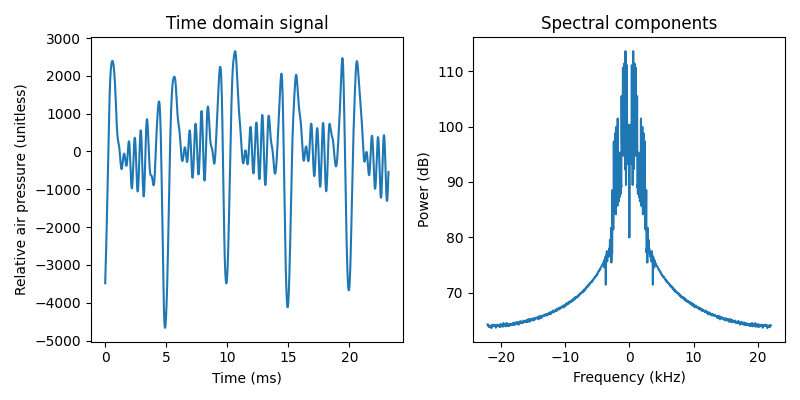
\includegraphics[width=\textwidth]{code/013_audio_spec/audio_spec.png}
\end{center}
\caption{The spectral components of an audio signal (guitar string plucked). Left: time domain signal $x(t)$, Right: The magnitude of the spectral components in decibel scale: $10\log_{10}(|c_k|^2)$.}
\label{fig:audio_spec}
\end{figure}

\newpage
\section{Exercises: Fourier Series}

\begin{enumerate}
\item A signal is defined as:
\begin{equation}
    x(t) = 7 \sin(3 \pi t + 0.2\pi) + 3 \cos(7 \pi t + 0.5\pi)  
\end{equation}
The independent variable $t$ is in units of seconds. 
\begin{enumerate}[a)]
    \item Express this signal in the form of Equation \ref{eq:general_spectrum}. What are the values of the coefficients $c_k \in \mathbb{C}$ and angular frequencies $\omega_k \in \mathbb{R}$?
    \item The coefficients $c_{k}$, satisfy $c_{-k}=c_{k}^{*}$, why?
    \item Show that this signal is periodic by showing that the frequencies of the individual frequency components are commensurable.
    \item Use Euclid's algorithm to find the fundamental angular frequency $\omega$. What is the fundamental frequency in units of hertz and rad/s?
    \item What is the fundamental period $T$ of this signal in seconds?
    \item We delay the signal $x(t)$ by 0.5 seconds $y(t) = x(t-\frac{1}{2})$. Write $y(t)$ in the following format:
\begin{equation}
    y(t) = 7 \sin(3\pi t + \phi_0) + 3 \cos(7\pi t + \phi_1)
\end{equation}
What are the values $\phi_0$ and $\phi_1$?
\item We create a new signal $z(t) = x(t) + e^{i \sqrt{2} t + 13}$. Why is the signal $z(t)$ no longer periodic with a finite period? Is the signal $z(t)$ real valued?
\end{enumerate}

\item A signal is defined as:
  \begin{equation}
    x(t) = e^{-i (6\pi  t + 0.3)}  + 4e^{i (60\pi  t + 0.42)} + 4e^{-i (60\pi t + 0.42)}  + e^{i (6\pi t + 0.3)} 
  \end{equation}
  The independent variable $t$ is in units of seconds. 
  \begin{enumerate}[a)]
%  \item Make a plot of the frequency components of the signal, similar to the one in Figure \ref{fig:exspecsin}.
  \item Why is this signal real valued?
    \item Is this signal periodic? If so, what is the fundamental angular frequency $\omega$ and the fundamental period $T$?
   \end{enumerate}


\item The Fourier series coefficients for a pulsed signal $x(t)$ with
  a fundamental period $T=1$ is described as:
  \begin{equation}
    c_k = \left\{\begin{array}{ccc}
    \frac{1}{10} & \mathrm{when} & k=0 \\
    \frac{1}{\pi k}e^{-i\frac{\pi}{10}  k }\sin\left(\frac{\pi}{10} k  \right) & \mathrm{otherwise}
    \end{array}
    \right.
  \end{equation}
  See Equations \ref{eq:pulsecoeff0} and \ref{eq:pulsecoeff1} for the derivation of the Fourier coefficients.
  \begin{enumerate}[a)]
  \item Plot the partial sum $x_N(t)$ of the Fourier series using $N=101$. You can use Listing \ref{lst:fourier_square_code} to help you out.
  \item What are the Fourier series coefficients for a signal delayed in time by $0.2$ seconds. Plot the partial sum to verify.
  \item What are the Fourier series coefficients for $y(t)=\frac{d}{dt}x(t)$? Make a plot to verify.
  \end{enumerate}
  
\end{enumerate}


\if 0
\section{Programming Exercise 1}

\begin{itemize}
\item[a)] 
Using Equation \ref{eq:dirac_comb_coeff}, implement a program that
calculates a partial sum approximation of a Dirac comb with
period of $T=0.5$ seconds. Use $N=50$ as the number of complex
exponential signals to include in the partial sum. Evaluate the signal
from t=0 to t=4 seconds at 10 kHz sample rate. Here's some partial
code, which almost does the job.
\begin{lstlisting}[language=Python,numbers=none]
# define the sample rate (Hz)
sample_rate=10000.0
# create time array 0 to 4 seconds
t=n.arange(4.0*sample_rate)/sample_rate
# initialize empty vector to hold Fourier series
sig=n.zeros(len(t),dtype=n.complex64)
N=50
for k in range(-N,N):
    sig+=...# complete this line
    
plt.plot(sig.real)
plt.plot(sig.imag)
plt.show()
\end{lstlisting}

\item[b)] Delay the signal by 0.1 seconds by applying an adjustment to the complex coefficients $c_k$. Use Equation \ref{eq:time_shift_phasor}. Plot the non-delayed and delayed signals in the same plot and verify that the signal is delayed by the right amount.
\end{itemize}


\fi

 \ifSpExerciseSol
 \newpage
\section{Suggested solutions: Fourier Series}

\begin{enumerate}
\item Let $x(t)$ be the signal 
$$x(t)=7\sin(3\pi t+0.2\pi)+3\cos(7\pi t+0.5\pi).$$

\begin{enumerate}[a)]
\item Have that
\begin{align*}
    \sin\theta&=\frac{1}{2i}(e^{i\theta}-e^{-i\theta}), \\
    \cos\theta&=\frac{1}{2}(e^{i\theta}+e^{-i\theta}).
\end{align*}
This gives
\begin{align*}
    x(t)&=\frac{7}{2i}(e^{i(3\pi t+0.2\pi)}-e^{-i(3\pi t+0.2\pi)})+ \frac{3}{2}(e^{i(7\pi t+0.5\pi)}+e^{-i(7\pi t+0.5\pi)}), \\
    &=\left(\frac{7}{2i}e^{i0.2\pi}\right)e^{i3\pi t}-\left(\frac{7}{2i}e^{-i0.2\pi}\right)e^{-i3\pi t} + \left(\frac{3}{2}e^{i0.5\pi}\right)e^{i7\pi t}+\left(\frac{3}{2}e^{-i0.5\pi}\right)e^{-i7\pi t},
\end{align*}
giving
$$c_{k}=\left(\frac{3}{2}e^{-i0.5\pi},-\frac{7}{2i}e^{-i0.2\pi},\frac{7}{2i}e^{i0.2\pi},\frac{3}{2}e^{i0.5\pi}\right)$$
for which the corresponding angular frequencies are
$$\omega_{k}=(-7\pi,-3\pi,3\pi,7\pi).$$

\item For any real signal, the Fourier coefficients satisfy $c_{-k}=c_{k}^{*}$ and $x(t)$ is real. 

\item The signal is periodic if $\omega_{i}/\omega_{j}\in\mathbb{Q}$ for every pair $i,j\in \{-7,-3,3,7\}$ with $i\neq j$. In this case every $\omega_{i}$ is an integer multiply of $\pi$, so every ratio is a rational number as all the $\pi$s cancel.

\item Using Euclid's algorithm we have:
\begin{align*}
    &(3\pi,7\pi) \\
    &(3\pi,7\pi-3\pi) \\
    &(3\pi,4\pi) \\
    &(3\pi,4\pi-3\pi) \\
    &(3\pi,\pi) \\
    &(3\pi-\pi,\pi) \\
    &(2\pi,\pi) \\
    &(2\pi-\pi,\pi) \\
    &(\pi,\pi)
\end{align*}
Hence the fundamental angular frequency is $\omega=\pi\ \text{rad/s}$. In units of hertz, we have that $\omega=2\pi f$, so
$$f=\frac{\omega}{2\pi}=\frac{\pi}{2\pi}=\frac{1}{2}.$$
Thus, the fundamental frequency is $f=1/2\ \text{Hz}$. 

\item If the fundamental angular frequency is $\omega=\pi$, then the fundamental period is related by $T=2\pi/\omega$, hence
$$T=\frac{2\pi}{\omega}=\frac{2\pi}{\pi}=2\ \text{seconds}.$$

\item Define a new signal $y(t)=x(t-\frac{1}{2})$. That is, we delay the signal $x(t)$ by $\frac{1}{2}$. We get
$$y(t)=7\sin(3\pi \left(t-\frac{1}{2}\right)+0.2\pi)+3\cos(7\pi \left(t-\frac{1}{2}\right)+0.5\pi).$$
Simplifying gives
$$y(t)=7\sin(3\pi t-1.3\pi)+3\cos(7\pi t-3\pi).$$
Hence $\phi_{0}=-1.3\pi$ and $\phi_{1}=-3\pi$. 

\item Define another signal $z(t)=x(t)+e^{i\sqrt{2}+13}$. This new signal is not commensurable since we have a factor of $\sqrt{2}$, the signal is also not real-valued since we don't have a corresponding complex conjugate pair. 
\end{enumerate}

\item Let $x(t)$ be a signal defined as
$$x(t)=e^{-i(6\pi t+0.3)}+4e^{i(60\pi t+0.42)}+4e^{-i(60\pi t+0.42)}+e^{i(6\pi t+0.3)},$$
where $t$ is measured in seconds. 
\begin{enumerate}[a)]
\item This signal is real-valued since we have two pairs, each with the same frequency, but different signs. Thus, the signal can be written as a real signal for which it takes the following form:
$$x(t)=8\cos(60\pi t+0.42)+2\cos(6\pi t+0.3).$$
\item In this case, we have the angular frequencies of $\omega_{1}=60\pi$ and $\omega_{2}=6\pi$ for which $\omega_{1}/\omega_{2}=60\pi/6\pi=10$. We get a rational number, so the signal is periodic. 
\item To find the fundamental angular frequency, we use Euclid's algorithm. This gives
\begin{align*}
    &(60\pi,6\pi) \\
    &(54\pi,6\pi) \\
    &(48\pi,6\pi) \\
    &(42\pi,6\pi) \\
    &(36\pi,6\pi) \\
    &(30\pi,6\pi) \\
    &(24\pi,6\pi) \\
    &(18\pi,6\pi) \\
    &(12\pi,6\pi) \\
    &(6\pi,6\pi) \\
\end{align*}
therefore the fundamental angular frequency is $6\pi$ in units of radians per second. 

\item The fundamental period is
$$T=\frac{2\pi}{\omega}=\frac{2\pi}{6\pi}=\frac{1}{3},$$
hence $T=\frac{1}{3}$ in units of seconds.
\end{enumerate}


\item Let the Fourier series coefficients of a periodic signal $x(t)$ with fundamental period $T=1$ be 
$$c_{k}=\begin{cases}
    \frac{1}{10}, \hspace{2.3cm}\quad k=0, \\
    \frac{1}{\pi k}e^{-i\frac{\pi}{10}k}\sin(\frac{\pi}{10}k),\quad \text{otherwise}.
\end{cases}$$

\begin{enumerate}[a)]
\item Using Python, we can implement a simple program for the partial sum with $N=101$. Listing \ref{code:7.3a} shows a way. 
\begin{lstlisting}[language=Python, caption=Suggested solution to a),label=code:7.3a]
import numpy as n
import matplotlib.pyplot as plt

T = 1

sample_rate = 1000.0
t = n.arange(int(sample_rate*T))/sample_rate

xn = n.zeros(len(t),dtype=n.complex64)

N = 101

def ck(k):
    if k == 0:
        return 1/10
    else:
        return 1/(n.pi*k)*n.exp(-1j*n.pi*k/10)*n.sin(n.pi*k/10)

for i in range(-N,N+1):
    xn += ck(i)*n.exp(1j*2*n.pi*i*t/T)

plt.plot(t,xn.real,color="blue")
plt.plot(t,xn.imag,color="red")
plt.xlabel("Time (t)")
plt.ylabel("$x_{N}(t)$")
plt.show()
\end{lstlisting}

\item The Fourier coefficients of a delayed signal are related to the undelayed signal by $c_{k}'=e^{-i\frac{2\pi k\tau}{T}}c_{k}$. 
The script in Listing \ref{code:7.3a} can be modified to account for delay. The delayed version is shown in Listing \ref{code:7.3b}
\begin{lstlisting}[language=Python, caption=Suggested solution to b),label=code:7.3b]
import numpy as n
import matplotlib.pyplot as plt

T = 1
tau = 0.2 # delay

sample_rate = 1000.0
t = n.arange(int(sample_rate*T))/sample_rate

xn = n.zeros(len(t),dtype=n.complex64)

N = 101

def ck(k):
    if k == 0:
        return 1/10
    else:
        return 1/(n.pi*k)*n.exp(-1j*n.pi*k/10)*n.sin(n.pi*k/10)

for i in range(-N,N+1):
    xn += ck(i)*n.exp(1j*2*n.pi*i*(t-tau)/T)

plt.plot(t,xn.real,color="blue")
plt.plot(t,xn.imag,color="red")
plt.xlabel("Time (t)")
plt.ylabel("$x_{N}(t)$")
plt.show()
\end{lstlisting}

\item Define $y(t)=\frac{d}{dt}x(t)$. If $c_{k}$ are the Fourier coefficients for $x(t)$, then the Fourier coefficients for $y(t)$ is
$$d_{k}(t)=i \frac{2\pi k}{T}c_{k}.$$
Using Python we have Listing \ref{code:7.3c}.
\begin{lstlisting}[language=Python, caption=Suggested solution to c),label=code:7.3c]
import numpy as n
import matplotlib.pyplot as plt

T = 1
tau = 0.0 # delay

sample_rate = 1000.0
t = n.arange(int(sample_rate*T))/sample_rate

xn = n.zeros(len(t),dtype=n.complex64)

N = 101

def ck(k):
    if k == 0:
        return 1/10
    else:
        return 1/(n.pi*k)*n.exp(-1j*n.pi*k/10)*n.sin(n.pi*k/10)

for i in range(-N,N+1):
    xn += (1j*2*n.pi*i/T)*ck(i)*n.exp(1j*2*n.pi*i*(t-tau)/T)

plt.plot(t,xn.real,color="blue")
plt.plot(t,xn.imag,color="red")
plt.xlabel("Time (t)")
plt.ylabel("$y_{N}(t)$")
plt.show()
\end{lstlisting}
\end{enumerate}







\end{enumerate}
 \fi
\newpage
\section{Audio Compression Example [Optional]}
In this application example, I'll show you how to estimate the
spectral components of an audio signal and how this can be used for
audio compression. I won't go very deep into either of these
topics. The main idea is to expose you to these concepts.

\newthought{Example: audio compression algorithms often use a sparse spectral
representation of an audio signal}.  The sounds produced by musical
instruments when playing a single note are often good examples of
periodic signals that occur in our daily life. Of course, real signals
are typically not exactly periodic, but for short intervals this
approximation is good.

A good example of this is the signal shown in
Figure \ref{fig:audio_spec}, which depicts the sound signal (instantaneous
relative air pressure at the microphone) emitted by a guitar when one
string is plucked.

A Fourier series approximation of an audio signal is often used in
audio compression, as it is often possible to approximate an audio
signal relatively accurately with relatively few non-zero Fourier
series coefficients. This is the basic idea behind the MP3 audio
compression algorithm\sidenote[][0em]{Yes, there is more to it. Note, that
real world compression algorithms use a lot more tricks, such as
psychoacoustics -- not storing spectral components that humans cannot
hear very well in music. These are outside the scope of this basic
course on signal processing though. However, it is already possible to
achieve significant compression just using the simple idea of
representing the signal only using the $N$ largest amplitude spectral
components. I would wager that most of the compression is achieved
with the sparse spectral representation.}.

The Python code in Listing \ref{lst:audio_compression} demonstrates
audio compression in practice. Understanding the program may require
you to be somewhat familiar with analyzing what computer programs
do. If you are just starting with programming, feel free to skip going
through this program example.

The audio compression example program relies on the discrete Fourier
transform (FFT), which we haven't covered yet. Just think of
the \verb|numpy.fft.fft| operation as the analysis step of the Fourier
series, which gives you the phase and amplitude of each frequency
component $c_k$. We'll cover the discrete Fourier transform in more
detail at a later part of this course.

\lstinputlisting[language=Python,caption={\texttt{010\_audio\_compression/audio\_compression.py}},label=lst:audio_compression]{code/010_audio_compression/audio_compression.py}

The algorithm discards weak spectral components of the signal and
stores the strong ones. This can result in significant savings in
storage space. In this example, the amount of storage required is only
5\% of the original audio signal!


\newpage
\section{Image Compression Example}
\newthought{The Fourier series can be generalized to two-dimensional
  signals $I:\mathbb{R}^2 \rightarrow \mathbb{C}$}. The two
dimensional Fourier series is often used in image processing and image
compression.

The Fourier series representation for a two dimensional periodic
function with period $T_x$ in the $x$ direction and $T_y$ in the $y$
direction is:
\begin{equation}
I(x,y) = \sum_{n,m \in \mathbb{Z}} c_{n,m} e^{i \frac{2\pi}{T_x}nx} e^{i \frac{2\pi}{T_y}my} \,\,.
\end{equation}
The analysis procedure to obtain the coefficients $c_{n,m}\in \mathbb{C}$ is:
\begin{equation}
c_{n,m} = \frac{1}{T_x T_y}\int_{0}^{T_x}\int_0^{T_y} I(x,y) e^{-i \frac{2\pi}{T_x}nx} e^{-i \frac{2\pi}{T_y}my}dx dy \,\,.
\label{eq:2d_analysis}
\end{equation}
Many of the familiar results for 1d signals, such as the time shifting
property, or differentiation, can be extended to 2d or higher
dimensional periodic functions. 
%All of the results regarding differentiation and ``time shifting'' can
%be generalized to multiple dimensions. For example, time shift in two
%dimensions $I(x+\tau_x,y+\tau_y)$ is equivalent to translation in $x$
%and $y$, and this operation can be applied directly on the constants
%$c_{n,m}$.


\newthought{In this programming example I'll briefly demonstrate to
  you the concept of spectral image compression}.  It is possible to
extend the idea of compression of a one dimensional signal, as
demonstrated in the audio compression example, by only storing strong
frequency components in 2D images. This is essentially the idea
behind the JPEG image compression algorithm.  The Python code in
Listing \ref{lst:image_compression} demonstrates image compression and
produces the image shown in Figure \ref{fig:image_compression}. The
program uses the 2D discrete-Fourier transform function,
\verb|numpy.fft.fft2|, to calculate the phases and amplitudes of the
spectral components, $c_{n,m}$, of the image. It then uses the 2D
inverse discrete Fourier transform to FFT synthesize an image from
only 5\% of the spectral components. The output of the image
compression example is shown in Figure \ref{fig:image_compression}. It
shows the original and compressed image that is formed using a sparse
Fourier series representation of the image. The magnitudes of the
spectral components for the compressed and original image are also
shown.

\begin{figure}
\begin{center}
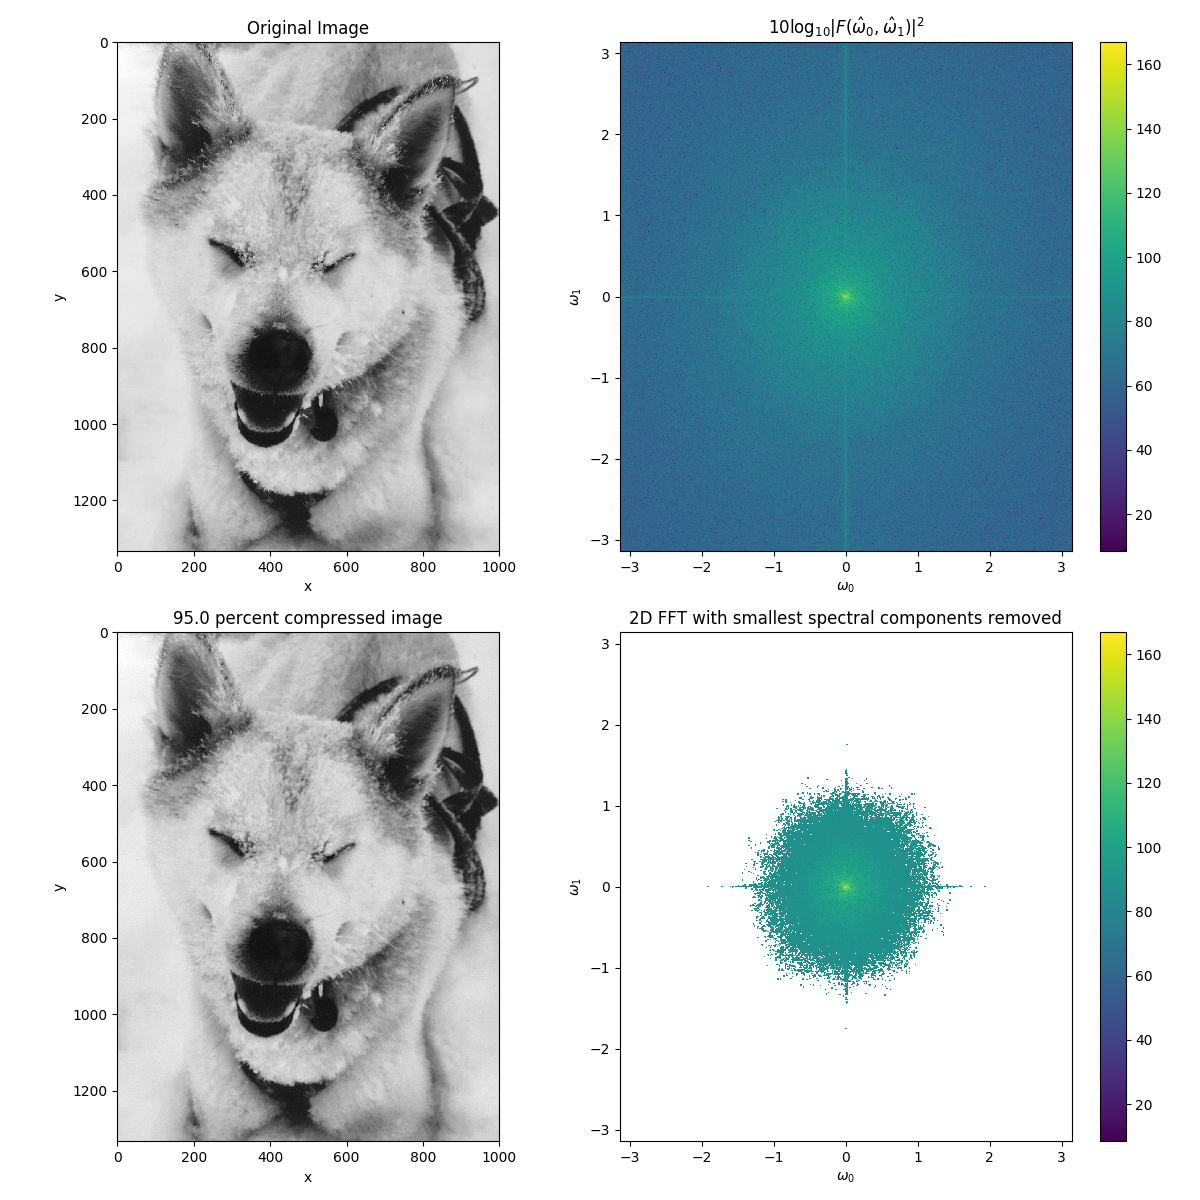
\includegraphics[width=0.93\textwidth]{Applications/figures/image_compression.png}
\end{center}
\caption{Image compression example. Top left: original image, Top
  right, the magnitude squared of the spectral components in dB
  scale. Bottom left: compressed image formed using only 5\% of the
  strongest spectral components. Bottom right: the spectral magnitude
  squared of the spectral components used to form the image on the
  bottom left.}
\label{fig:image_compression}
\end{figure}

The same words of warning that I gave with the audio compression
example apply to this program example. If you are only beginning with
Python, you may have a hard time with understanding this program. For now, you can think of the 2D FFT and inverse FFT as an analysis and synthesis step for a 2D
periodic function. But don't let a warning or lack of experience
prevent you from exploring!

\lstinputlisting[language=Python,caption={\texttt{011\_image\_compression/image\_compression.py}},label=lst:image_compression]{code/011_image_compression/image_compression.py}

%Equation \ref{eq:dirac_comb_coeff} provides the formula for the phase and amplitude of each spectral component of a Dirac comb signal. What does this result tell you about how power is distributed over frequency?

%\item Using Section \ref{dirac_section}, implement a program that calculates a partial sum approximation of a Dirac delta train with period $T=0.5$ seconds. Use $N=50$ as the number of complex exponential signals to include in the partial sum. Evaluate the signal from t=0 to t=4 seconds at 10 kHz sample rate. Here's some partial code, which almost does the job. 
%\begin{lstlisting}[language=Python,numbers=none]
%# determine sample rate (Hz) sample_rate=10000.0 # create time array 0
%to 4 seconds t=n.arange(4.0*sample_rate)/sample_rate # initialize
%empty vector to hold Fourier series
%sig=n.zeros(len(t),dtype=n.complex) N=50 for k in range(-N,N): sig+=
%...
%    
%plt.plot(sig.real)
%plt.show()
%\end{lstlisting}
%\item[b)] Delay the signal by 0.1 seconds by applying a phasor term to the Fourier series coefficients, with the help of Section \ref{delay_section}. Plot the undelayed and delayed signals in the same plot and verify that the signal is delayed by the right amount.
%\end{itemize}

%\if
\newpage
\section{Variable star lightcurve fitting}
\newthought{Example: The study of astronomical light curves of variable stars is an example of a practical application of the Fourier series}.

Variable stars called Cepheids, have intensities $I(t)$ that varies
periodically as a function of time. An example of a light curve is
shown in Figure \ref{fig:cepheid_lightcurve}. Such variable stars
pulsate in luminosity in a regularly repeating manner. The repeating
luminosity waveform is often very non-sinusoidal, necessitating a
Fourier series analysis.

\begin{marginfigure}
\begin{center}
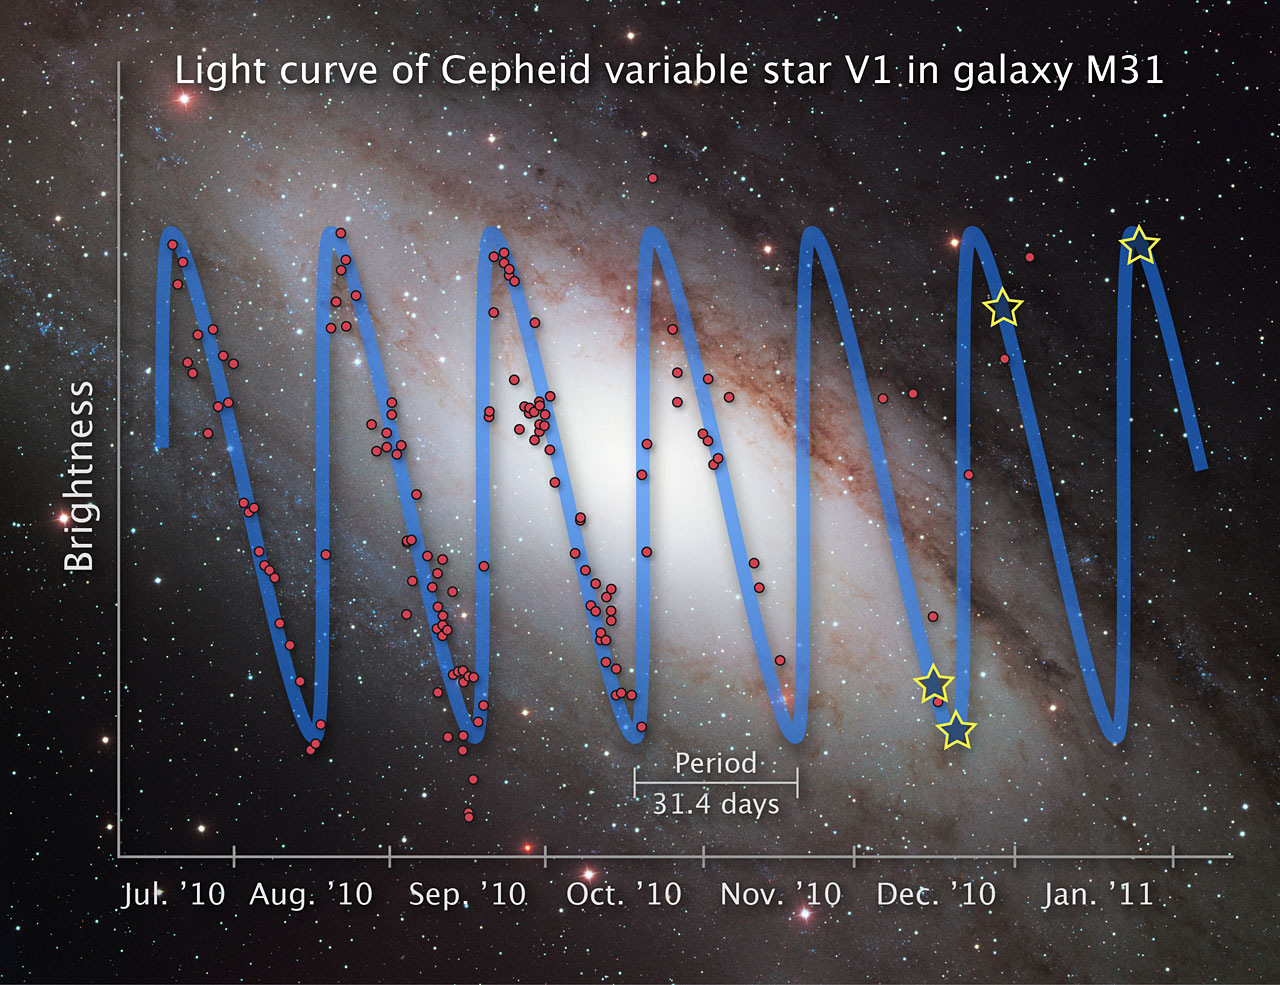
\includegraphics[width=\textwidth]{Applications/figures/ceph.jpg}
\end{center}
\caption{Measurements of the intensity of a variable star (red) and a Fourier series model of the intensity of the star as a function of time (blue). Illustration Credit: NASA, ESA and Z. Levay (STScI). Science Credit: NASA, ESA, the Hubble Heritage Team (STScI/AURA) and the American Association of Variable Star Observers.}
\label{fig:cepheid_lightcurve}
\end{marginfigure}

Measurements of the intensity of a Cepheid variable star are made at
periods of time when telescope time is available and astronomical
seeing allows observations to be made. The time spacing between
measurements is therefore by no means regular.

When analyzing the periodic waveform of this star, a search is made to
determine the period $T$ of the intensity waveform, and the Fourier
series coefficients $c_k$. This is done by using an exhaustive search
for plausible values of $T$. The model function is a Fourier series
synthesis equation:
\begin{equation}
I_N(t) = \sum_{k=-N}^N c_k e^{i\frac{2\pi}{T}kt} \,\,.
\end{equation}
The relationship between absolute brightness and the pulsation
frequency (fundamental frequency) is thought to be relatively
stable. This makes these types of variable stars useful for measuring
the astronomical distances.


The Fourier series can be used to express periodic functions. One real
life use case is estimating the functional form for a periodic star,
which varies in brightness periodically. In this exercise, we will
determine the Fourier series coefficients for brightness observations
of a real Cepheid star. We will then plot the Fourier series for the
periodic light curve of this star.

To estimate the periodic waveform for a Cepheid variable star
brightness measurements $m(t)$, we will use something called the
maximum likelihood method, which estimates the Fourier series
coefficients.  This involves expressing the Fourier series as a matrix
vector operation:
\begin{align}
m &= A x\\
\begin{bmatrix}
m(t_0)\\
m(t_1)\\
m(t_2)\\
\vdots \\
m(t_{M})
\end{bmatrix} &=
\begin{bmatrix}
e^{i\frac{2\pi}{T} k_0 t_0} & e^{i\frac{2\pi}{T} k_1 t_0} & \hdots & e^{i\frac{2\pi}{T} k_N t_0} \\
e^{i\frac{2\pi}{T} k_0 t_1} & e^{i\frac{2\pi}{T} k_1 t_1} & \hdots & e^{i\frac{2\pi}{T} k_N t_1} \\
\vdots & \vdots & \ddots & \vdots \\
e^{i\frac{2\pi}{T} k_0 t_M} & e^{i\frac{2\pi}{T} k_1 t_M} & \hdots & e^{i\frac{2\pi}{T} k_N t_M} 
\end{bmatrix} 
\begin{bmatrix}
c_0 \\
c_1 \\
c_2 \\
\vdots \\
c_N
\end{bmatrix}  \,\,.
\end{align}
Here $c_k$ is a Fourier series coefficient and $T$ is the fundamental
period. Because there are discrete measurements, the measurement
function is only known at discrete points $m(t_{\ell})$. In order to
estimate the Fourier series coefficients, we use the linear
least-squares estimator:
\begin{equation}
\hat{x} = (A^H A)^{-1}A^H m \,\,.
\end{equation}
The vector $\hat{x}$ will now contain the most probable Fourier series
coefficients that explain the measurements $m(t_{\ell})$ of the
periodic function.

Because this course does not deal with statistics, we have implemented
the code that figures out the Fourier series coefficients that fit the
measurements. Your task is to edit the code below, and to evaluate the
Fourier series model, given the coefficients $c_k$, which are in the
array variable named \verb|c_k|. Code is shown in Listing
\ref{lst:variable_star}, which already does most of the work. Complete
the last for-loop, and you should get the following plot:
\begin{center}
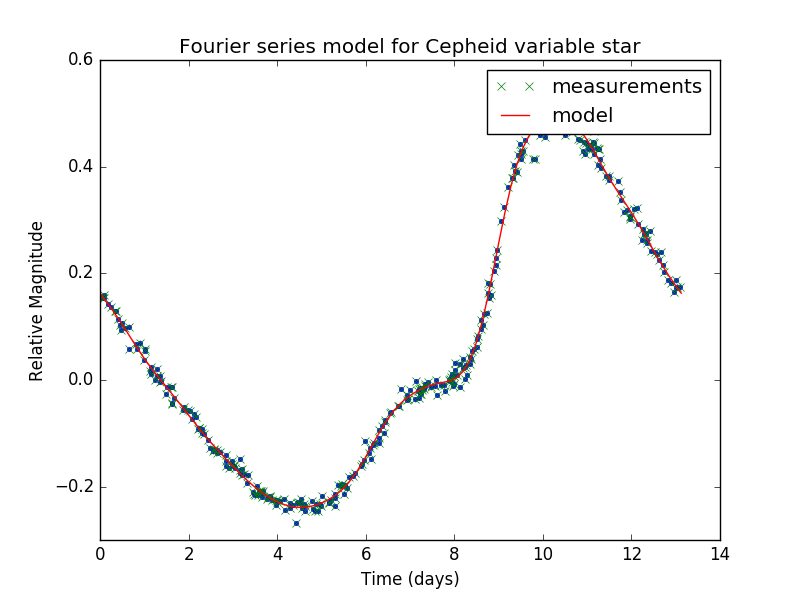
\includegraphics[width=0.92\textwidth]{Applications/figures/ceph.png}
\end{center}

\lstinputlisting[language=Python,caption={\texttt{012\_variable\_star/variable\_star.py}},label=lst:variable_star]{code/012_variable_star/variable_star.py}



\fi

\ifSpProgA
\chapter{Programming Assignment 1}

Perform the following tasks. Write a report describing your results,
which is \textbf{at most two pages long}. The report is free form, but
it must be delivered in PDF format. Include your code and plots in the
report. The report should be delivered by the deadline to the
following location using your candidate ID number:
\url{http://kaira.uit.no/juha/upload/}

The Dirac comb is a periodic signal, which is defined as follows:
\begin{equation}
x(t) = \sum_{k=-\infty}^{\infty} \delta(t - k T)
\end{equation}
The signal is shown in Figure \ref{fig:dirac_comb_plot}.

\begin{marginfigure}
\begin{center}
\begin{tikzpicture}
\pgfmathdeclarefunction{p}{1}{%
  \pgfmathparse{(and(mod(#1,2)>0, mod(#1,2)<1))}%
} \begin{axis}[
width=7cm,
axis lines = center,
ymax=1.5,
ymin=0,
xmax=3.5,
xmin=-3.5,
legend pos=outer north east,
yticklabels={,,},
xticklabels={,,},
xlabel={$t$},
ylabel={$x(t)$}
]
    
    \addplot+[ycomb,color=blue,mark=triangle*,mark options={blue}] plot coordinates {
    (-3,1)
    (-2,1)
    (-1,1)
    (-0,1)
    (1,1)
    (2,1)
    (3,1)
};

\node at (axis cs:1.5,1.15) {$\displaystyle{T}$};   
\addplot [dimen] plot coordinates {(1,1.1) (2,1.1)};

    \end{axis}
\end{tikzpicture}
\end{center}
\caption{The Dirac comb signal with period $T$.}
\label{fig:dirac_comb_plot}
\end{marginfigure}


\begin{itemize}
\item[a)] Implement a program that calculates a partial sum
  approximation
  \begin{equation}
    x_N(t) = \sum_{k=-N}^{N} c_k e^{i \frac{2\pi}{T}kt}
    \label{eq:fs_pt1_eq}
\end{equation}
  of a Dirac comb with a fundamental period of $T=0.55$ seconds. Use
  $N=50$ in Equation \ref{eq:fs_pt1_eq} to define the number of
  complex exponential signals to include in the sum. Evaluate the
  signal from $t=0$ to $t=4$ seconds at 10 kHz sample rate.

  Here's some partial code, which almost does the
  job, but has several things wrong.
\begin{lstlisting}[language=Python, numbers=none]
import matplotlib.pyplot as plt
import numpy as np
# Define the sample rate (Hz).
sample_rate = 10000.0
# Create time array 0 to 1 seconds.
t = np.arange(1.0*sample_rate)/sample_rate
# Initialize empty vector to hold Fourier series.
sig = np.zeros(len(t), dtype=np.complex64)
N = 10
# Add together complex sinusoids multiplied with Fourier series coefficients.
for k in range(-N, N):
    print(k)
    sig += ... # Complete this line.
    
plt.plot(t, sig.real)
plt.plot(t, sig.imag)
plt.xlabel("Time (s)")
plt.show()
\end{lstlisting}
If implemented correctly, the Fourier series should be real-valued. 
The imaginary part should only deviate from zero by only a
very small number due to numerical errors in finite precision
accuracy of floating point numbers.
  
\item[b)] Figure out what modification you need to make to the Fourier series coefficients $c_k$ in order to delay the signal by 0.2 seconds.

\item[c)] Plot and verify that the coefficients obtained in b) produce the correct delay.


\end{itemize}

\fi

\ifSpFourierTra
\chapter{Fourier Transform}
This chapter discusses the continuous-time Fourier transform. We'll cover the following topics:
\begin{itemize}
    \item Important Fourier transform pairs
    \item Plancherel's theorem and Parseval's theorem 
    \item Convolution theorem
    \item Impulse response and frequency response of LTI systems
    \item Fourier transform of a time shifted signal
\end{itemize}

\noindent The \emph{\index{forward Fourier transform}{forward Fourier transform}} is defined as:
\begin{equation}
\boxed{
\hat{x}(\omega) = \int_{-\infty}^{\infty} x(t) e^{-i\omega t}dt}
\end{equation}
and the \emph{\index{inverse Fourier transform}{inverse Fourier transform}} is defined as:
\begin{equation}
\boxed{
x(t) = \frac{1}{2\pi}\int_{-\infty}^{\infty} \hat{x}(\omega) e^{i\omega t}d\omega\,\,.
}
\end{equation}
We'll use the following notation to indicate Fourier transform pairs:
\begin{equation}
\boxed{x(t) \xleftrightarrow{\mathcal{F}} \hat{x}(\omega)\,\,.}
\end{equation}
The left denotes the \emph{\index{time domain}{time domain}} representation of the signal and the right-hand side denotes the \emph{\index{frequency domain}{frequency domain}} representation of the same signal. 
I've used a hat to signify that the symbol $\hat{x}(\omega)$ is a frequency domain representation of a signal.

The existence or non-existence of a Fourier transform or an inverse Fourier transform is rarely something that is encountered in signal processing applications. Exploring this topic rigorously is outside the scope of this course.

\section{Selected Fourier transforms}
It is impossible to exhaustively cover all the possible Fourier transform pairs here. We'll only give examples of commonly encountered Fourier transforms and provide solution strategies for using these as basic building blocks to evaluate the Fourier transform for more complicated signals. Refer to a formula book\sidenote{The wikipedia article also contains a nice table of Fourier transform pairs:\url{https://en.wikipedia.org/wiki/Fourier_transform}.}\cite{kammler2007first} for a more complete table of Fourier transform pairs.

\subsection{Linear combination}
The Fourier transform of a linear combination of signals in time domain is related to a linear combination of Fourier transforms in frequency domain:
\begin{equation}
\boxed{
y(t)=c_1 x_1(t)  + c_2 x_2(t) \xleftrightarrow{\mathcal{F}} \hat{y}(\omega) = c_1\hat{x}_1(\omega)+c_2\hat{x}_2(\omega)\,\,.
}
\end{equation}
This can be shown as follows:
\begin{align}
\hat{y}(\omega) &= \int_{-\infty}^{\infty} [c_1 x_1(t)+c_2 x_2(t)] e^{-i\omega t} dt \\
&= c_1\int_{-\infty}^{\infty} x_1(t) e^{-i\omega t} dt + c_2\int_{-\infty}^{\infty} x_2(t) e^{-i\omega t} dt \\ 
&=  c_1\hat{x}_1(\omega)+c_2\hat{x}_2(\omega)\qed\,\,.
\end{align}
This may seem trivial, but keep this property in mind, as it can be used to Fourier transform more complicated signals that are a superposition of simple individual signals.

\subsection{Fourier transform of $\delta(t+\tau)$}

\begin{marginfigure}
\begin{center}
        \begin{tikzpicture}
        \begin{axis}[width=6cm,height=4cm,ymin=0,xmin=0,ymax=1.1,xmax=2,         
        yticklabels={,,},
        xtick={1},
        ytick={0},
        xticklabels={$-\tau$},
        xlabel=$t$,
        ylabel={$x(t)=\delta(t+\tau)$}, 
        axis lines = center]

\addplot +[dirac] coordinates {(1,0.8)};
%\node at (axis cs:1.25,1) [below, font={\footnotesize}]{$\delta(t+\tau)$};

\end{axis}
        \end{tikzpicture}

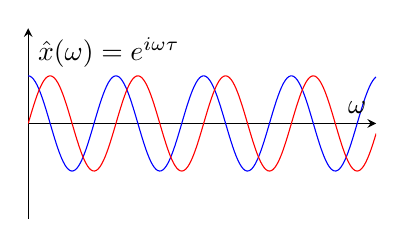
\begin{tikzpicture}
	\begin{axis}[domain=0:(2*6.23),
        width=6cm,
        height=4cm,
        ticks=none,
        axis lines = center,
        ymax=2,
        ymin=-2,
        samples=200,
        legend pos=north east,
        legend style={draw=none},
        xlabel={$\omega$},
        ylabel={$\hat{x}(\omega)=e^{i\omega \tau}$}]
    \addplot[blue] {cos(2*deg(x))};
    \addplot[red] {sin(2*deg(x))};
%    \node at (axis cs:3.14,-1.5) {$\displaystyle{T=\frac{2\pi}{\omega}}$};   
%    \addplot [dimen] plot coordinates {(1.57,-1.1) (4.71,-1.1)};   
%    \legend{$\mathrm{Re}(e^{i\omega t})$,$\mathrm{Im}(e^{i\omega t})$}
    \end{axis}
\end{tikzpicture}
\end{center}
\caption{Unit impulse signal $\delta(t+\tau)$ is non-zero only when $t=-\tau$. In frequency domain, the Fourier transform is a complex sinusoidal signal with $\omega$ the independent variable.}
\end{marginfigure}


The time shifted unit impulse signal is a complex sinusoidal signal in frequency domain:
\begin{equation}
\boxed{
  x(t)=\delta(t+\tau) \xleftrightarrow{\mathcal{F}} \hat{x}(\omega) = e^{i\omega \tau}\,\,.
  \label{eq:fttss}
}
\end{equation}
This is also relatively easy to show:
\begin{align}
\hat{x}(\omega) &= \int_{-\infty}^{\infty} x(t) e^{-i\omega t} dt \\
&= \int_{-\infty}^{\infty} \delta(t+\tau) e^{-i\omega t} dt \\
&= e^{i\omega \tau} \qed\,\,.
\end{align}

\subsection{Fourier transform of $e^{i\omega_0 t}$}


\begin{marginfigure}
\begin{center}

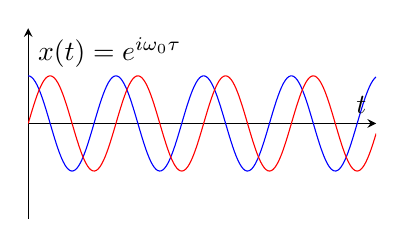
\begin{tikzpicture}
\begin{axis}[domain=0:(2*6.23),
        width=6cm,
        height=4cm,
        ticks=none,
        axis lines = center,
        ymax=2,
        ymin=-2,
        samples=200,
        legend pos=north east,
        legend style={draw=none},
        xlabel={$t$},
        ylabel={$x(t) =e^{i\omega_0 \tau}$}]
    \addplot[blue] {cos(2*deg(x))};
    \addplot[red] {sin(2*deg(x))};
    \end{axis}
\end{tikzpicture}

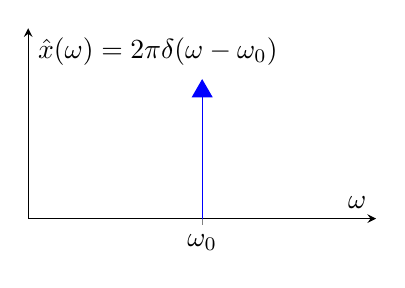
\begin{tikzpicture}
        \begin{axis}[width=6cm,height=4cm,ymin=0,xmin=0,ymax=1.1,xmax=2,         
        yticklabels={,,},
        xtick={1},
        ytick={0},
        xticklabels={$\omega_0$},
        xlabel=$\omega$,
        ylabel={$\hat{x}(\omega)=2\pi \delta(\omega-\omega_0)$}, 
        axis lines = center]

\addplot +[dirac] coordinates {(1,0.8)};
\end{axis}
\end{tikzpicture}
\end{center}
\caption{A complex sinusoidal signal of frequency $\omega_0$ is a unit impulse signal $\delta(\omega-\omega_0)$ in frequency domain.}
\end{marginfigure}

The converse of the previous is a complex sinusoidal signal $e^{i\omega_0 t}$ with frequency $\omega_0$. This has the following Fourier transform pair:
\begin{equation}
\boxed{
x(t) = e^{i\omega_0 t} \xleftrightarrow{\mathcal{F}} \hat{x}(\omega) = 2\pi \delta(\omega-\omega_0)\,\,.
}
\end{equation}
We show this by inverse Fourier transforming $\hat{x}(\omega)$:
\begin{align}
x(t) &= \frac{1}{2\pi}\int_{-\infty}^{\infty} \hat{x}(\omega) e^{i\omega t} d\omega \\
 &= \frac{1}{2\pi}\int_{-\infty}^{\infty} 2\pi \delta(\omega-\omega_0)e^{i\omega t} d\omega \\
 &= e^{i\omega_0 t}\qed\,\,.
\end{align}

\subsection{Rectangular function}
One often encountered Fourier transform pair is that of the rectangular function\footnote{Also often called the boxcar function.} of length $T$:
\begin{equation}
\boxed{
x(t)=u\left(t+\frac{T}{2}\right) - u\left(t-\frac{T}{2}\right) \xleftrightarrow{\mathcal{F}} \hat{x}(\omega) = \frac{1}{i\omega}(e^{i\omega \frac{T}{2}} - e^{-i\omega \frac{T}{2}})\,\,.
}
\end{equation}

This can be derived as follows:
\begin{align}
\hat{x}(\omega) &= \int_{-\infty}^{\infty} \left[u\left(t+\frac{T}{2}\right) - u\left(t-\frac{T}{2}\right)\right] e^{-i\omega t}dt \\
&= \int_{-T/2}^{T/2} e^{-i\omega t}dt\\
&=  \left.-\frac{e^{-i\omega t}}{i\omega} \right|_{t=-T/2}^{T/2}\\
&= \frac{e^{i\omega \frac{T}{2}}- e^{-i\omega \frac{T}{2}}}{i\omega}\,\,.
\end{align}
We can use Euler $\sin(x) = \frac{1}{2i} (e^{i x} - e^{-ix})$ to express this as follows:

\begin{marginfigure}
\begin{center}

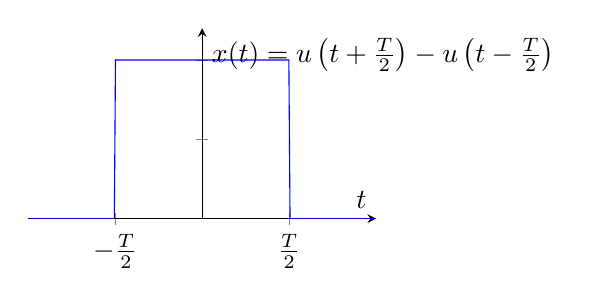
\begin{tikzpicture}
	\begin{axis}[domain=(-1):(1),samples=300,
        width=6cm,
        height=4cm,
    ymin=0,ymax=1.2,
        xlabel={$t$},
        ylabel={$x(t)=u\left(t+\frac{T}{2}\right) - u\left(t-\frac{T}{2}\right)$},
        axis x line=center, 
        axis y line=center, 
        yticklabels={,,,}, 
        xtick={-0.5,0.5},
        xticklabels={$-\frac{T}{2}$,$\frac{T}{2}$}
    ]

    \addplot[blue] {(x>-0.5)*(x<0.5)};
\end{axis}
\end{tikzpicture}

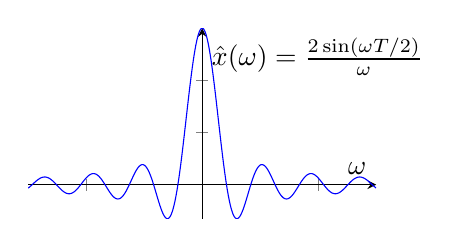
\begin{tikzpicture}
	\begin{axis}[domain=(-15):(15),samples=300,
        width=6cm,
        height=4cm,        
        xlabel={$\omega$},
        ylabel={$\hat{x}(\omega)=\frac{2\sin(\omega T/2)}{\omega}$},
        axis x line=center, 
        axis y line=center, 
        yticklabels={,,,}, 
        xticklabels={,,,}
    ]
    \addplot[blue] {2*sin(0.5*3*deg(x))/x};
\end{axis}
\end{tikzpicture}
\end{center}
\caption{The Fourier transform of a boxcar function.}
\end{marginfigure}

\begin{equation}
\boxed{
\hat{x}(\omega) = \frac{2\sin(\omega \frac{T}{2})}{\omega}\,\,.
}
\end{equation}
The function $\mathrm{sinc}(\omega)=\sin(\pi\omega)/(\pi\omega)$ is often used to express this function. This is convenient, as numerical implementations (such as \verb|numpy.sinc|) of the function deal with the special case when $\omega=0$, which can be investigated using L'H\^{o}pital's rule:
\begin{equation}
\lim_{\omega \rightarrow c} \frac{f(\omega)}{g(\omega)} = \lim_{\omega \rightarrow c} \frac{f'(\omega)}{g'(\omega)}\,\,.
\end{equation}
Which in this case is:
\begin{equation}
\lim_{\omega \rightarrow 0} \frac{2\sin(\omega T/2)}{\omega} = \lim_{\omega \rightarrow 0} T\cos(\omega T/2 ) = T\,\,.
\end{equation}
We'll be using L'H\^{o}pital's rule elsewhere in signal processing to resolve similar situations.

\subsection{Sinc function}
A related Fourier transform pair is the one where the frequency domain representation is a rectangular function. This is used, e.g., when calculating ideal filters. 
This result is also used in Shannon's sampling theorem to obtain an ideal reconstruction filter for band limited signals that only have spectral components in the band
$|\omega| < \omega_b$.
\begin{equation}
\boxed{
x(t) = \frac{\sin(\omega_b t)}{\pi t} \xleftrightarrow{\mathcal{F}} \hat{x}(\omega) = u(\omega+\omega_b) - u(\omega-\omega_b)\,\,.
}
\label{eq:ft:sinc}
\end{equation}
This relationship can be shown by inverse Fourier transforming $\hat{x}(\omega)$:
\begin{align}
x(t) &= \frac{1}{2\pi}\int_{-\infty}^{\infty} \left[u(\omega+\omega_b) - u(\omega-\omega_b)\right] e^{i\omega t}d\omega \\
 &= \frac{1}{2\pi}\int_{-\omega_b}^{\omega_b} e^{i\omega t}d\omega \\
 &= \frac{1}{2\pi}\left.\frac{e^{i\omega t}}{it}\right|_{\omega=-\omega_b}^{\omega_b} \\
 &= \frac{e^{i t \omega_b} - e^{-i t \omega_b} }{ 2\pi i t} \\
 &= \frac{\sin(\omega_b t)}{\pi t}\qed\,\,.
\end{align}
Fourier transforming the sinc-function is not as trivial.

\begin{marginfigure}
\begin{center}
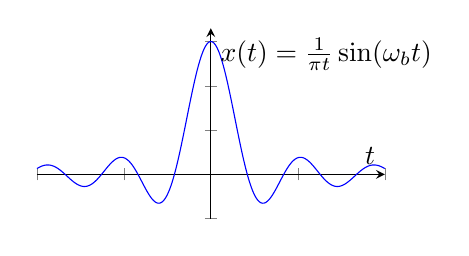
\begin{tikzpicture}
	\begin{axis}[
        width=6cm,
        height=4cm,
        domain=(-10):(10),
        samples=300,
        ymin=-1,
        ymax=3.3,
        xlabel={$t$},
        ylabel={$x(t)=\frac{1}{\pi t}\sin(\omega_b t)$},
        axis x line=center, 
        axis y line=center, 
        yticklabels={,,,}, 
        xticklabels={,,,}
    ]
    \addplot[blue] {2*sin(0.5*3*deg(x))/x};
\end{axis}
\end{tikzpicture}

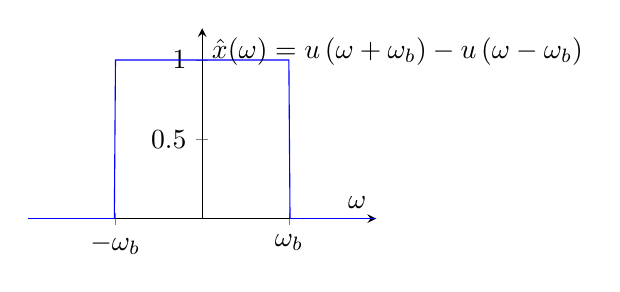
\begin{tikzpicture}
	\begin{axis}[
        width=6cm,
        height=4cm,
        domain=(-1):(1),
        samples=300,
        ymin=0,
        ymax=1.2,
        xlabel={$\omega$},
        ylabel={$\hat{x}(\omega) = u\left(\omega+\omega_b\right) - u\left(\omega-\omega_b\right)$},
        axis x line=center, 
        axis y line=center, 
        xtick={-0.5,0.5},
        xticklabels={$-\omega_b$,$\omega_b$}
    ]
    \addplot[blue] {(x>-0.5)*(x<0.5)};
\end{axis}
\end{tikzpicture}
\end{center}
\caption{A sinc function in time domain is a boxcar function in frequency domain.}
\end{marginfigure}

\subsection{Gaussian}
The Fourier transform of a Gaussian density function is another Gaussian density function:
\begin{equation}
\boxed{x(t) = e^{-\alpha t^2} \xleftrightarrow{\mathcal{F}} \sqrt{\frac{\pi}{\alpha}} e^{-\frac{\omega^2}{4\alpha}}\,\,.}
\end{equation} 
Note that the width of the time domain Gaussian is inversely proportional to the width of the frequency domain Gaussian.

If we rewrite the above into a form which resembles a Gaussian density function normalized to unity at zero, with a width parameter $\sigma_t$ and $\sigma_\omega$ for the time domain and frequency domain width, we get:
% 4*a = 1/2s**2.0
\begin{equation}
x(t) \propto e^{-\frac{t^2}{2\sigma_t^2}} \xleftrightarrow{\mathcal{F}} \hat{x}(\omega) \propto e^{-\frac{\omega^2}{2\sigma_\omega^2}}\,\,,
\end{equation}
which implies that:
\begin{equation}
\frac{1}{\sigma_t} = \sigma_\omega\,\,.
\end{equation}%$\alpha=(1/2)*s_t^2$
This is a very nice demonstration of the inverse relationship between the width of a signal in time domain and frequency domain. 
When we discuss filters later on, we'll use this to show that the length of a filter in time domain is inversely proportional to the spectral resolution (width of the filter response).

\begin{marginfigure}
\begin{center}
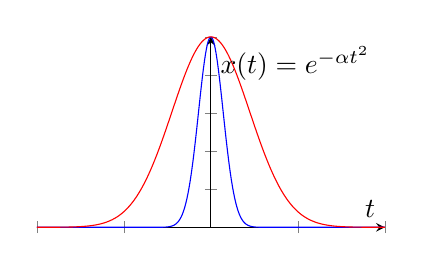
\begin{tikzpicture}
	\begin{axis}[
        width=6cm,
        height=4cm,
        domain=(-10):(10),
        samples=300,
        xlabel={$t$},
        ylabel={$x(t)=e^{-\alpha t^2}$},
        axis x line=center, 
        axis y line=center, 
        yticklabels={,,,}, 
        xticklabels={,,,}
    ]
    \addplot[blue] {exp(-x*x)};
        \addplot[red] {exp(-0.1*x*x)};

\end{axis}
\end{tikzpicture}

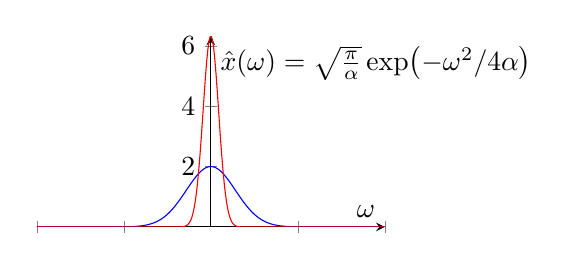
\begin{tikzpicture}
	\begin{axis}[
        width=6cm,
        height=4cm,
        domain=(-10):(10),
        samples=300,
        xlabel={$\omega$},
        ylabel={$\hat{x}(\omega) = \sqrt{\frac{\pi}{\alpha}}\exp(-\omega^2/4\alpha)$},
        axis x line=center, 
        axis y line=center, 
        xticklabels={,,,}
    ]
    \addplot[blue] { sqrt(4)*exp(-x*x/4)) };
        \addplot[red] { sqrt(4/0.1)*exp(-x*x/(4*0.1))) };
\end{axis}
\end{tikzpicture}
\end{center}
\caption{The Fourier transform of a Gaussian density function is another Gaussian density function. The width of the frequency domain and time domain density functions are inversely proportional.}
\label{fig:gaussftf}
\end{marginfigure}

This Fourier transform pair can be derived as follows:
\begin{align}
\hat{x}(\omega) &= \int_{-\infty}^{\infty} e^{-\alpha t^2} e^{-i\omega t} dt \\
&= \int_{-\infty}^{\infty} e^{-\alpha t^2 - i\omega t} dt\,\,.
\end{align}
We perform a little trick and multiply with $1=e^{c^2\omega^2}e^{-c^2\omega^2}$ using a procedure called completing the square, so that we can get to a variable substitution that allows us to easily integrate the function inside the integral:
\begin{align}
\hat{x}(\omega) &= e^{c^2 \omega^2}\int_{-\infty}^{\infty} e^{-\alpha t^2 -i\omega t - c^2 \omega^2} dt\,\,.
\end{align}
We now substitute a variable $\alpha'=\sqrt{\alpha}$. We then need to find a constant $c$ so that:
\begin{equation}
-t^2\alpha'^2 - i\omega t - c^2 \omega^2 = -(t \alpha' + c\omega)^2\,\,.
\end{equation}
We find that $c=\frac{i}{2\alpha'}$.% t**2a**2 + 2*t*a*c*o + c**2*o**2, c = i/(2a)
\begin{equation}
\hat{x}(\omega) = e^{-\frac{\omega^2}{4\alpha}} \int_{-\infty}^{\infty} e^{-\left(t\alpha' + \frac{i}{2\alpha'}\omega\right)^2} dt\,\,.
\end{equation}
Now we perform a variable substitution: $u=t\alpha' + \frac{i}{2\alpha'}\omega$, which gives us: $\frac{1}{\alpha'}du = dt$. 

We now need to refer to a table of integrals to obtain a solution to the integral:
\begin{align}
\int_{-\infty}^{\infty} e^{-u^2} du &= \sqrt{\pi}
\end{align}
and thus
\begin{align}
\hat{x}(\omega) &= \frac{1}{\sqrt{\alpha}}e^{-\frac{\omega^2}{4\alpha}} \int_{-\infty}^{\infty} e^{-u^2} du\\
&=\sqrt{\frac{\pi}{\alpha}} e^{-\frac{\omega^2}{4\alpha}}\,\,.
\end{align}
The plots in Figure \ref{fig:gaussftf} show the time domain and frequency domain Fourier transform pairs for two different values of $\alpha$, which demonstrates the inverse relationship between the width of the function in time and frequency domain.

\subsection{Exponentially decaying signal $x(t) = e^{-\beta t}u(t)$}

\begin{marginfigure}
\begin{center}
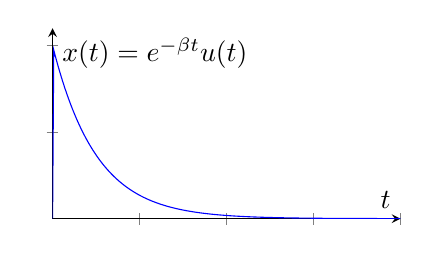
\begin{tikzpicture}
	\begin{axis}[domain=(0):(4),samples=300,
                width=6cm,
        height=4cm,
    ymin=0,ymax=1.1,
        xlabel={$t$},
        ylabel={$x(t)=e^{-\beta t} u(t)$},
        axis x line=center, 
        axis y line=center, 
        yticklabels={,,,}, 
        xticklabels={,,,}
    ]
    \addplot[blue] {(x>0)*exp(-2*x)};
\end{axis}
\end{tikzpicture}

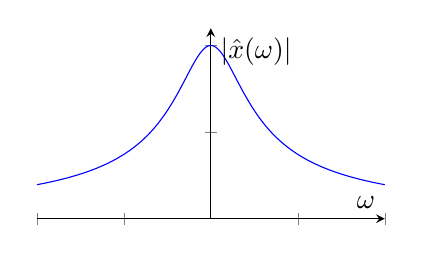
\begin{tikzpicture}
	\begin{axis}[domain=(-10):(10),samples=300,
        width=6cm,
        height=4cm,
    ymin=0,ymax=1.1,
        xlabel={$\omega$},
        ylabel={$|\hat{x}(\omega)|$},
        axis x line=center, 
        axis y line=center, 
        yticklabels={,,,}, 
        xticklabels={,,,}
    ]
    \addplot[blue] {abs(2/sqrt(4+x*x))};
\end{axis}
\end{tikzpicture}

\end{center}
\caption{The Fourier transform of an exponentially decaying signal.}
\end{marginfigure}

When $\beta \in \mathbb{R}_{>0}$ the signal $e^{-\beta t} u(t)$ decays exponentially. 
This type of signal is often encountered in electrical circuits (e.g., a low pass filter) and in control systems:
\begin{equation}
\boxed{x(t)=e^{-\beta t} u(t) \xleftrightarrow{\mathcal{F}} \hat{x}(\omega)=\frac{1}{\beta + i\omega}\,\,.}
\end{equation}
This can be derived as follows:
\begin{align}
\hat{x}(\omega) &= \int_{-\infty}^{\infty} e^{-\beta t} u(t) e^{-i\omega t}dt \\
&= \int_{0}^{\infty} e^{-(\beta+i\omega) t} dt \\
&= \left. -\frac{1}{\beta + i\omega} e^{-(\beta + i\omega)t} \right|_{t=0}^{\infty}\\
&= \frac{1}{\beta + i\omega}\,\,.
\end{align}
The above requires that $\beta \in \mathbb{R}_{> 0}$.

\subsection{Real-valued signals}
There is a special conjugate symmetry for signals that are real-valued either in time domain or frequency domain. 

If the time domain signal is real-valued, then the frequency domain representation is conjugate symmetric.
\begin{equation}
\boxed{
x(t) \in \mathbb{R} \xleftrightarrow{\mathcal{F}} \hat{x}(-\omega)=\hat{x}^*(\omega)\,\,.
}
\end{equation}
The same also applies the other way around. If the spectral representation is real-valued, then the time domain representation is conjugate symmetric:
\begin{equation}
\boxed{
x(-t)=x^*(t) \xleftrightarrow{\mathcal{F}} \hat{x}(\omega) \in \mathbb{R}\,\,.
}
\end{equation}
This can be shown as follows:
\begin{proof}
\begin{align}
\hat{x}^*(\omega) &= \left(\int_{-\infty}^{\infty} x(t) e^{-i\omega t}dt\right)^* \\
 &= \int_{-\infty}^{\infty} x^*(t) e^{i\omega t}dt \\
 &= \int_{-\infty}^{\infty} x(t) e^{i\omega t}dt \\
 &= \hat{x}(-\omega)\,\,.
\end{align}
\end{proof}
Because $x(t)\in\mathbb{R}$, we have that $x^*(t)=x(t)$. A similar proof exists for the real-valued spectral representation. 
% This same property exists for all the spectral representations.

\subsection{Fourier series}
A Fourier series can be used to represent a periodic function as a sum of frequency components. Because we know that the Fourier transform of $e^{i\omega' t}$ is $2\pi\delta(\omega-\omega')$, we can easily determine the Fourier transform of an arbitrary periodic function by using its Fourier series:
\begin{equation}
\boxed{
x(t) = \sum_{k=-\infty}^{\infty} c_k e^{i k \omega_0 t} \xleftrightarrow{\mathcal{F}} \hat{x}(\omega) = 2\pi \sum_{k=-\infty}^{\infty}  c_k \delta(\omega-k\omega_0)\,\,.\label{eq:fsftgen}
}
\end{equation}
The derivation is as follows:
\begin{align}
\hat{x}(\omega) &= \int_{-\infty}^{\infty} \sum_{k=-\infty}^{\infty} c_k e^{ik\omega_0 t} e^{-i\omega t} dt\\
&= \sum_{k=-\infty}^{\infty} c_k\int_{-\infty}^{\infty} e^{ik\omega_0 t}e^{-i\omega t}dt\\
&= 2\pi\sum_{k=-\infty}^{\infty}  c_k \delta(\omega - k\omega_0)\,\,.
\end{align}
This is simply the continuous-frequency representation of Fourier series spectral components. 
A periodic function has non-zero spectral components only at frequencies that are multiples of $\omega_0$. 
\begin{marginfigure}
\begin{center}
        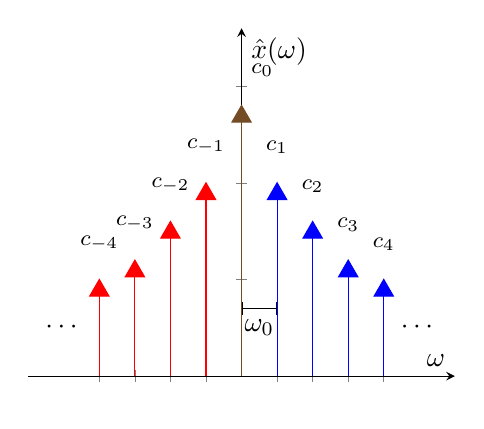
\begin{tikzpicture}
        \begin{axis}[width=7cm,
        height=6cm,
        ymin=-0,
        xmin=-3,
        ymax=1.8,
        xmax=3,
        yticklabels={,,},
        xtick={-2,-1.5,-1,-0.5,0,0.5,1.0,1.5,2},
        xticklabels={,,},%$-4 \omega_0$,$-3\omega_0$,$-2 \omega_0$,$-\omega_0$,$0$,$ \omega_0$,$2 \omega_0$,$3 \omega_0$,$4 \omega_0$},
    xlabel=$\omega$,
    ylabel=$\hat{x}(\omega)$,
    axis lines = center]
    
   \addplot+[dirac] plot coordinates {(0.5,1) (1.0,0.8) (1.5,0.6) (2,0.5)};
    \addplot+[dirac] plot coordinates {(-0.5,1) (-1.0,0.8) (-1.5,0.6) (-2,0.5)};
   \addplot+[dirac] plot coordinates {(0.0, 1.4)};
    \node at (axis cs:-2.5,0.25) {$\cdots$};   
    \node at (axis cs:2.5,0.25) {$\cdots$};   
    \node at (axis cs:0.25,0.25) {$\omega_0$};   
    
       
    \addplot [dimen] plot coordinates {(0.0,0.35) (0.5,0.35)};

    \node at (axis cs:0.0,1.5) [above right, font={\footnotesize}]{$c_0$};
    \node at (axis cs:0.5,1.1) [above, font={\footnotesize}]{$c_1$};
    \node at (axis cs:1.0,0.9) [above, font={\footnotesize}]{$c_2$};
    \node at (axis cs:1.5,0.7) [above, font={\footnotesize}]{$c_3$};
    \node at (axis cs:2.0,0.6) [above, font={\footnotesize}]{$c_4$};

    \node at (axis cs:-0.5,1.1) [above, font={\footnotesize}]{$c_{-1}$};
    \node at (axis cs:-1.0,0.9) [above, font={\footnotesize}]{$c_{-2}$};
    \node at (axis cs:-1.5,0.7) [above, font={\footnotesize}]{$c_{-3}$};
    \node at (axis cs:-2.0,0.6) [above, font={\footnotesize}]{$c_{-4}$};
\end{axis}
        \end{tikzpicture}
\end{center}
\caption{The Fourier transform of a Fourier series. The spectral representation is a set of spectral lines spaced apart by $\omega_0$, the fundamental angular frequency of the periodic signal. 
A set of spectral lines spaced apart by a constant value is a spectral signature of a time-periodic signal.}
\end{marginfigure}

\begin{marginfigure}
\begin{center}
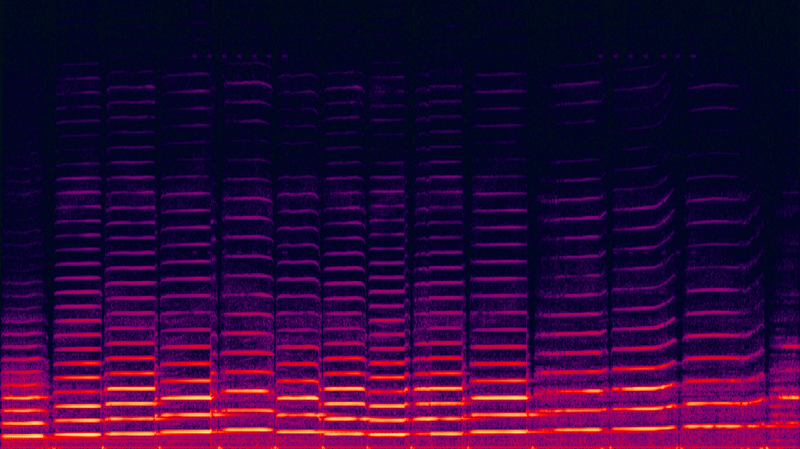
\includegraphics[width=\textwidth]{ch08/figures/real_spectrum.png}
\end{center}
\caption{A time-frequency-power image of a violin being played. The x-axis represents time and the y-axis represents frequency. 
Only positive frequencies are shown. At any given moment, a violin is playing approximately a time-periodic signal (a single note).  The spectrum is a forest of spectral lines spaced apart by the fundamental angular frequency of the signal.  Credits: Wikipedia.}
\end{marginfigure}

The inverse Fourier transform of the spectrum $\hat{x}(\omega)$ is:
\begin{align}
x(t) &= \frac{1}{2\pi}\int_{-\infty}^{\infty} \hat{x}(\omega)e^{i\omega t} d\omega \\
&= \sum_{k=-\infty}^{\infty} c_k \int_{-\infty}^{\infty} \delta(\omega - k\omega_0) e^{i\omega t} d\omega \\
&= \sum_{k=-\infty}^{\infty} c_k e^{ik\omega_0 t}\,\,.
\end{align}
The fact that the continuous-time Fourier transform and the Fourier series are related in this way shouldn't be too surprising, 
as we earlier derived the Fourier transform from the Fourier series representation for a periodic function with an infinitely long fundamental period.

\subsection{Time scaling system}
Let's look at a time scaling system:
\begin{equation}
y(t) = x(at)\,\,.
\end{equation}
What effect does this system have on the frequency domain representation of this signal?

We assume that a signal $x(t)$ has a Fourier transform:
\begin{align}
x(t) \xleftrightarrow{\mathcal{F}} \hat{x}(\omega)\,\,.
\end{align}
If we scale the time parameter $x(at)$, then the spectral representation is scaled inversely in frequency:
\begin{align}
\boxed{
  y(t) = x(at) \xleftrightarrow{\mathcal{F}} \hat{y}(\omega) = \frac{1}{|a|}\hat{x}\left(\frac{\omega}{a}\right)\,\,.
  \label{eq:timescale_ft_pair}
}
\end{align}
What does scaling in time mean?
\begin{itemize}
\item compressing a signal in time with $|a|>1$ will stretch the signal in frequency.
\item stretching a signal in time with $|a|<1$ will compress the signal in frequency. 
\end{itemize}
\begin{proof}
The proof is as follows. Let's investigate the case where $a > 0$ and Fourier transform $y(t)$:
\begin{align}
\hat{y}(\omega) &= \int_{-\infty}^{\infty} y(t) e^{-i\omega t}dt\\
                &= \int_{-\infty}^{\infty} x(at) e^{-i\omega t}dt\,\,.
\end{align}
We do a variable substitution $t'=at$, from which it follows that $dt=\frac{1}{a}dt'$ and 
\begin{align}
\hat{y}(\omega) &= \frac{1}{a}\int_{-\infty}^{\infty} x(t') e^{-i\frac{\omega}{a} t' }dt'\\
 &= \frac{1}{a}\hat{x}\left(\frac{\omega}{a} \right)\,\,.
\end{align}
\end{proof}


%If $a\rightarrow 0$, the $x(at) \rightarrow c$ approaches a constant and $\frac{1}{a}\hat{x}(i\frac{\omega}{a})$ approaches a Dirac-delta $c\delta(\omega)$.

%If $a\rightarrow \infty$, then $x(at)$ is compressed in time and the function $\hat{x}(\omega) \rightarrow $




\subsection{Plancherel's theorem}

Plancherel's theorem states that for any two signals $f(t)$ and $g(t)$ with Fourier transforms $\hat{F}(\omega)$ and $\hat{G}(\omega)$ the following integral is satisfied:
\begin{equation}
\boxed{
\int_{-\infty}^{\infty} f(t) g^*(t) dt = \frac{1}{2\pi} \int_{-\infty}^{\infty}  \hat{F}(\omega)\hat{G}^*(\omega) d\omega\,\,.
}
\label{eq:ft_plancherel_theorem}
\end{equation}
This is useful, as we can relate the amount of signal power in time domain to the total amount of power in frequency domain. This theorem has many applications in, e.g., the 
theory of random processes, radio astronomical signal processing, and radar signal processing.


\begin{proof}
The proof is as follows. Consider first the following signal, which is represented using the Dirac delta function in frequency domain:
\begin{equation}
\hat{x}(\omega) = \delta(\omega-\omega')\,\,.
\end{equation}
This has a time domain-representation, which is obtained using the inverse Fourier transform:
\begin{align}
x(t) &= \frac{1}{2\pi} \int_{-\infty}^{\infty} \delta(\omega-\omega')e^{i\omega t}d\omega \\
     &= \frac{1}{2\pi} e^{i\omega' t}\,\,.
\end{align}
Let us now consider the Fourier transform representations for these two signals:
\begin{align}
f(t) &= \frac{1}{2\pi} \int_{-\infty}^{\infty} F(\omega) e^{i\omega t}d\omega \\
g(t) &= \frac{1}{2\pi} \int_{-\infty}^{\infty} G(\omega') e^{i\omega' t}d\omega'\,\,.
\end{align}
If we multiply the Fourier representations of these two and integrate over time:
\begin{align}
\int_{-\infty}^{\infty} f(t)g^*(t)dt &= \frac{1}{(2\pi)^2} \int_{-\infty}^{\infty}  \left[\int_{-\infty}^{\infty} F(\omega) e^{i\omega t}d\omega \right] \left[ \int_{-\infty}^{\infty} G^*(\omega') e^{-i\omega' t}d\omega' \right]dt\\
&= \frac{1}{(2\pi)^2} \int_{-\infty}^{\infty} F(\omega) \int_{-\infty}^{\infty} G^*(\omega') \int_{-\infty}^{\infty} e^{i(\omega-\omega')t}dt d\omega' d\omega\\
&=\frac{1}{2\pi} \int_{-\infty}^{\infty} F(\omega) \int_{-\infty}^{\infty} G^*(\omega') \delta(\omega-\omega') d\omega' d\omega \\
&=\frac{1}{2\pi} \int_{-\infty}^{\infty} F(\omega) G^*(\omega)  d\omega \,\,.
\end{align}
\end{proof}
The key to this proof is that:
\begin{align}
\int_{-\infty}^{\infty} e^{i(\omega-\omega')t}dt &= \int_{-\infty}^{\infty} e^{-i\omega' t} e^{i\omega t} dt = 2\pi \delta(\omega - \omega')\,\,.
\end{align}


\newthought{Parseval's theorem} is simply a corollary of Plancherel's theorem. If we state that $f(t)=g(t)=x(t)$, then Plancherel's theorem becomes:
\begin{equation}
\boxed{
\int_{-\infty}^{\infty} |x(t)|^2 dt = \frac{1}{2\pi} \int_{-\infty}^{\infty} | \hat{x}(\omega)|^2 d\omega\,\,.
}
\end{equation}
In physics this means that the total energy of the signal in time domain and frequency domain is equivalent, up to a predefined fixed scaling constant. 


\subsection{Convolution theorem}
The convolution theorem states that a convolution operation in time domain is a multiplication operation in frequency domain. A convolution sum of signals $x_1(t)$ and $x_2(t)$ is defined as:
\begin{equation}
\boxed{
x_1(t)*x_2(t) := \int_{-\infty}^{\infty} x_1(\tau) x_2(t-\tau)d\tau\,\,.
}
\end{equation}
The star symbol ($*$) is often used in shorthand to express this operation.

An often used property in signal processing is that convolution in time domain is multiplication in frequency domain.
\begin{equation}
\boxed{
y(t) =
x_1(t)*x_2(t) \xleftrightarrow{\mathcal{F}} \hat{y}(\omega)=\hat{x}_1(\omega)\hat{x}_2(\omega)\,\,.
}
\end{equation}



\begin{proof}
\begin{align}
\hat{y}(\omega) &= \int_{-\infty}^{\infty} y(t) e^{-i\omega t} dt \\
                 &= \int_{-\infty}^{\infty} \left( \int_{-\infty}^{\infty} x_1(\tau) x_2(t-\tau) d\tau \right) e^{-i\omega t} dt \\
                 &= \int_{-\infty}^{\infty}   x_1(\tau) \left( \int_{-\infty}^{\infty} x_2(t-\tau) e^{-i\omega t} dt \right) d\tau \,\,.
\end{align}
Next, we perform substitution of variables $m=t-\tau$. From this, it follows that $t=m+\tau$ and $dm=dt$. After substitution, we get:
\begin{align}
\hat{y}(\omega)&= \int_{-\infty}^{\infty}   x_1(\tau) \left( \int_{-\infty}^{\infty} x_2(m) e^{-i\omega m} dm \right) e^{-i\omega \tau} d\tau  \\
                &= \hat{x}_2(\omega) \int_{-\infty}^{\infty}   x_1(\tau)  e^{-i\omega \tau} d\tau  \\
                &= \hat{x}_1(\omega)\hat{x}_2(\omega)\,\,.
\end{align}
\end{proof}
\newthought{The converse of the previous is that multiplication in time domain corresponds to convolution in frequency domain}:
\begin{equation}
\boxed{
y(t) = x_1(t)x_2(t) \xleftrightarrow{\mathcal{F}} \hat{y}(\omega) = \frac{1}{2\pi}\hat{x}_1(\omega) * \hat{x}_2(\omega)\,\,.
}
\end{equation}
\begin{proof}
We start by Fourier transforming $x_1(t)x_2(t)$:
\begin{align}
\hat{y}(\omega) &= \int_{-\infty}^{\infty} x_1(t) x_2(t) e^{-i\omega t} dt \,\,.
\end{align}
We then substitute $x_2(t)$ with its Fourier transform:
\begin{align}
x_2(t) = \frac{1}{2\pi}\int_{-\infty}^{\infty} \hat{x}_2(\omega') e^{i\omega' t}d\omega'\,\,,
\end{align}
which gives us:
\begin{align}
\hat{y}(\omega) &= \int_{-\infty}^{\infty} x_1(t) \left(\frac{1}{2\pi}\int_{-\infty}^{\infty} \hat{x}_2(\omega') e^{i\omega' t} d\omega' \right) e^{-i\omega t} dt\,\,.
\end{align}
We then swap the order of integration and combine all terms with $t$ inside the innermost integral:
\begin{align}
\hat{y}(\omega)   &= \frac{1}{2\pi} \int_{-\infty}^{\infty} \hat{x}_2(\omega')  \left(\int_{-\infty}^{\infty}  x_1(t) e^{i\omega' t} e^{-i\omega t} dt  \right) d\omega'  \\
    &= \frac{1}{2\pi} \int_{-\infty}^{\infty} \hat{x}_2(\omega')  \left(\int_{-\infty}^{\infty}  x_1(t) e^{-{i(\omega-\omega')t}} dt  \right) d\omega'  \\
    &= \frac{1}{2\pi} \int_{-\infty}^{\infty} \hat{x}_2(\omega')  \hat{x}_1\left(\omega-\omega'\right) d\omega'  \\
    &= \frac{1}{2\pi}\hat{x}_1(\omega )  *\hat{x}_2(\omega)\,\,.
\end{align}
\end{proof}
This property is also very useful. We will use it next to inspect the spectrum of an amplitude modulated signal. This property will also be used when deriving Shannon's sampling theorem.

\section{Time shifted signal}
Assuming that the Fourier transform of $x(t)$ is $\hat{x}(\omega)$, the Fourier transform of a \index{time shifted signal} time shifted signal can be obtained using the following formula:
\begin{equation}
\boxed{y(t) = x(t-t_0) \xleftrightarrow{\mathcal{F}} \hat{y}(\omega)= e^{-i\omega t_0}\hat{x}(\omega)\,\,.}
\label{eq:ft:timeshift}
\end{equation}
\begin{proof}
Left as an exercise.
\end{proof}

\subsection{Alternative definitions and notation}
There are several notations and slightly different definitions of a Fourier transform that one may encounter in the literature. 
These mainly vary in how the frequency parameter of the spectral representation is scaled and what symbols are used to denote frequency and the imaginary number. 
The underlying mathematical concepts are the same. 

The spectral representation is sometimes written with an explicit function parameter $i\omega$ instead of $\omega$. Sometimes the hat-notation is not used:
\begin{equation}
\hat{x}(\omega) = \hat{x}(i\omega) = x(\omega)\,\,.
\end{equation}
Commonly used symbols for frequency include $\omega$, $\nu$, $\xi$, $\lambda$, $k$, $l$, and $f$. Also, as usual, the imaginary number $i=\sqrt{-1}$ is sometimes denoted with $j$.

The most common alternative form is the one where the frequency parameter is given scaled to units of cycles per unit of $t$:
\begin{equation}
f = \frac{\omega}{2\pi}\,\,.
\end{equation}
If $t$ is in units of time in seconds, then the units of $f$ would be $1/s$ or hertz. With this frequency parameterization, the transform is unitary (it is norm preserving):
\begin{align}
\hat{x}_1(f) &=  \int_{-\infty}^{\infty} x(t) e^{-i 2\pi f  t}d t\\
x(t) &= \int_{-\infty}^{\infty} \hat{x}_1(f) e^{i 2\pi f t} d f\,\,.
\end{align}
Another commonly used definition for the Fourier transform is one where the forward and reverse transform are scaled symmetrically:
\begin{align}
\hat{x}_2(\omega) &= \frac{1}{\sqrt{2\pi}} \int_{-\infty}^{\infty} x(t) e^{-i\omega t}dt \label{eq:ft_alt_form}\\
x(t) &= \frac{1}{\sqrt{2\pi}} \int_{-\infty}^{\infty} \hat{x}_2(\omega) e^{i\omega t}d\omega\,\,.
\end{align}
Sometimes, the sign convention for the forward and reverse transform is changed:
\begin{align}
\hat{x}_3(\omega) &=  \int_{-\infty}^{\infty} x(t) e^{i\omega t}dt\\
x(t) &= \frac{1}{2\pi} \int_{-\infty}^{\infty} \hat{x}_3(\omega) e^{-i\omega t}d\omega\,\,.
\end{align}
All of these alternative Fourier transform definitions have the same general properties, but the exact equations can differ in scaling constants or in sign of the frequencies. 
For example, if we were to define the Fourier transform as in equation \ref{eq:ft_alt_form}, the Fourier transform of $x(t)=\delta(t+\tau)$ would be $\hat{x}(\omega)=\frac{1}{\sqrt{2\pi}}e^{i\omega \tau}$, 
which is slightly different from the result we obtained in Equation \ref{eq:fttss}.

\if 0
The Laplace transform:
\begin{equation}
  F(s) = \int_{-\infty}^{\infty} f(t) e^{-st} dt
\end{equation}
is related to the Fourier transform. When $s=i\omega$, the above integral evaluates to the Fourier transform. We will not discuss this transform further in this course, but it is useful to 
\fi

\newpage
\section*{Exercises: Fourier Transform}
\begin{enumerate}
\item A rectangular signal is defined as:
\begin{equation}
    x(t) = u\left(t+1\right)-u\left(t-1\right)
\end{equation}
\begin{enumerate}[a)]
\item Sketch a plot of $x(t)$. How long is the rectangular pulse $x(t)$?
\item This signal is scaled in time as follows $y(t) = x(2t)$. Sketch a plot of the signal $y(t)$. How long is the rectangular pulse $y(t)$?
\item Evaluate the Fourier transforms of these functions: $\hat{x}(\omega)=\mathcal{F}\{x(t)\}$ and $\hat{y}(\omega)=\mathcal{F}\{y(t)\}$ using the definition of the Fourier transform.
\item How wide are the sinc functions $\hat{x}(\omega)$ and $\hat{y}(\omega)$? You can use e.g., the spacing between the first zero crossings of the sinc function as a measure of width. Does this agree with Equation \ref{eq:timescale_ft_pair}?
\end{enumerate}

\item Find the Fourier transforms of these signals:
\begin{enumerate}[a)]
\item $x(t)=\delta(t+2)+\delta(t)+\delta(t-2)$ \\Hint: linearity and time shift properties
\item $x(t)=\frac{\sin(100\pi [t-2])}{\pi (t-2)}$ \\Hint: time shift property
\item $x(t)=e^{-t}u(t) - e^{-t} u(t-4)$ \\Hint: look at the derivation for the Fourier transform of $e^{-\beta t} u(t)$
\end{enumerate}
Note that there are more than one way to solve the Fourier transforms!

\item Find the inverse Fourier transform for the following:
\begin{enumerate}[a)]
\item $\hat{x}(\omega)= 2 + \cos(\omega)$
\item $\hat{x}(\omega) = \frac{1}{1+i\omega} - \frac{1}{2+i\omega}$
\item $\hat{x}(\omega) = i \delta(\omega - 100\pi) - i\delta(\omega + 100\pi)$.
\end{enumerate}
  
\item Use known Fourier transform pairs together with the properties of the Fourier transform to complete the following Fourier transform pairs:
  \begin{enumerate}[a)]
  \item $x(t) = u(t+3)u(3-t) \xleftrightarrow{\mathcal{F}} \hat{x} = ?$
  \item $x(t) = \sin(4\pi t) \sin(50 \pi t)  \xleftrightarrow{\mathcal{F}} \hat{x} = ?$
  \item $x(t) = \frac{\sin(4\pi t)}{\pi t} \sin(50 \pi t)  \xleftrightarrow{\mathcal{F}} \hat{x} = ?$
  \item $x(t) = ?  \xleftrightarrow{\mathcal{F}} \hat{x} = \cos^2(\omega)$    
  \end{enumerate}


\item Let $\hat{x}(\omega)$ be the Fourier transform of $x(t)$. Prove that if $y(t)=x(t-\tau)$, then $\hat{y}(\omega)=e^{-i\tau}\hat{x}(\omega)$. 
  
  
  
  
\end{enumerate}

 \ifSpExerciseSol
 \newpage
\section{Suggested solutions: Fourier Transform}
\begin{enumerate}

\item
\begin{enumerate}[a)]
\item If:
$$x(t)=\delta(t+2)+\delta(t)+\delta(t-2),$$
then by linearity we have that:
$$\hat{x}(\omega)=\mathcal{F}\{x(t)\}=\mathcal{F}\{\delta(t+2)\}+\mathcal{F}\{\delta(t)\}+\mathcal{F}\{\delta(t-2)\},$$
now, by using time shift properties we get:
$$\hat{x}(\omega)=\mathcal{F}\{x(t)\}=\underline{\underline{e^{2i\omega}+1+e^{-2i\omega}}},$$
by Equation \ref{eq:fttss}.

\item Can rewrite the signal using the sinc function as:
$$x(t)=\frac{\sin(100\pi(t-2))}{\pi(t-2)}=100\text{sinc}(100(t-2)).$$
Then by Equation \ref{eq:ft:timeshift} and Equation \ref{eq:ft:sinc} the Fourier transform is:
$$\hat{x}(\omega)=100e^{-2i\omega}\mathcal{F}\{\text{sinc}100t\}=100e^{-2i\omega} \frac{1}{100}[u(\omega+100\pi)-u(\omega-100\pi)],$$
giving:
$$\hat{x}(\omega)=\underline{\underline{e^{-2i\omega}[u(\omega+100\pi)-u(\omega-100\pi)]}}.$$

\item Take:
$$x(t)=e^{-t}u(t)-e^{-t}u(t-4),$$
then by linearity, the Fourier transform is:
$$\hat{x}(\omega)=\mathcal{F}\{x(t)\}=\mathcal{F}\{e^{-t}u(t)\}-\mathcal{F}\{e^{-t}u(t-4)\}.$$
The last term can be computed as follows:
$$\mathcal{F}\{e^{-t}u(t-4)\} = \int_{-\infty}^{\infty}e^{-t}u(t-4)e^{-i\omega t}dt=\int_{4}^{\infty}e^{-t}e^{-i\omega t}dt=\int_{4}^{\infty}e^{-(1+\omega i)t}dt,$$
which gives:
$$\mathcal{F}\{e^{-t}u(t-4)\} = \left[-\frac{1}{1+i\omega}e^{-(1+i\omega)t}\right]_{4}^{\infty}=\frac{1}{1+i\omega}e^{-4(1+i\omega)}.$$
The first term is easily found as it is an exponential decay with $\beta=1$, giving:
$$\hat{x}(\omega)=\frac{1}{1+i\omega}-e^{-4(1+i\omega)}\frac{1}{1+i\omega}=\underline{\underline{\frac{1}{1+i\omega}\left(1-e^{-4(1+i\omega)}\right)}}.$$
\end{enumerate}

\item
\begin{enumerate}[a)]
\item Let $\hat{x}(\omega)=2+\cos\omega$, then the inverse Fourier transform is:
\begin{align*}
    x(t)&=\mathcal{F}^{-1}\{\hat{x}(\omega)\}=\mathcal{F}^{-1}\{2\}+\mathcal{F}^{-1}\{\cos\omega\}, \\
    &=2\delta(t)+\frac{1}{2}(\mathcal{F}^{-1}\{e^{i\omega}\}+\mathcal{F}^{-1}\{e^{-i\omega}\}), \\ 
    &=\underline{\underline{2\delta(t)+\frac{1}{2}(\delta(t+1)+\delta(t-1))}},
\end{align*}
as $\mathcal{F}^{-1}\{e^{i\omega\tau}\}=\delta(t+\tau)$.

\item For $\hat{x}(\omega)=\frac{1}{1+i\omega}-\frac{1}{2+i\omega}$, then the inverse Fourier transform is:
\begin{align*}
    x(t)&=\mathcal{F}^{-1}\{\hat{x}(\omega)\}=\mathcal{F}^{-1}\left\{\frac{1}{1+i\omega}\right\}-\mathcal{F}^{-1}\left\{\frac{1}{2+i\omega}\right\}, \\
    &=\underline{\underline{e^{-t}u(t)-e^{-2t}u(t)}},
\end{align*}
as $\mathcal{F}\{e^{-\beta t}u(t)\}=\frac{1}{\beta+i\omega}$. 

\item Let $\hat{x}(\omega)=i\delta(\omega-100\pi)-i\delta(\omega+100\pi)$, then the inverse Fourier transform is:
\begin{align*}
    x(t)&=\mathcal{F}^{-1}\{\hat{x}(\omega)\}=i\mathcal{F}^{-1}\{\delta(\omega-100\pi)\}-i\mathcal{F}^{-1}\{\delta(\omega+100\pi)\}, \\
    &=\frac{i}{2\pi}e^{100\pi it}-\frac{i}{2\pi}e^{-100\pi it}, \\
    &=\frac{1}{2\pi}(e^{i\pi/2}e^{100\pi i t}+e^{-i\pi/2}e^{-100\pi i t}), \\
    &=\underline{\underline{\frac{1}{\pi}\cos\left(100\pi t+\frac{\pi}{2}\right)}}.
\end{align*}
\end{enumerate}

\item   
\begin{enumerate}[a)]
\item Let $x(t)=u(t+3)u(3-t)$, then $x(t)$ is a rectangular function with corners at $t=\pm 3$ and height $1$. Therefore, we have:
$$\hat{x}(\omega)=\mathcal{F}\{x(t)\}=\int_{-\infty}^{\infty}u(t+3)u(3-t)e^{-i\omega t}dt=\int_{-3}^{3}e^{-i\omega t}dt=\left[\frac{1}{-i\omega}e^{-i\omega t}\right]_{t=-3}^{3}.$$
Evaluating this yields:
$$\hat{x}(\omega)=-\frac{1}{i\omega}(e^{-3i\omega}-e^{3i\omega})=\frac{1}{i\omega}(e^{3i\omega}-e^{-3i\omega})=\underline{\underline{\frac{2\sin(3\omega)}{\omega}}}.$$

\item Consider the signal $x(t)$ given as:
$$x(t)=\sin(4\pi t)\sin(50\pi t),$$
then:
\begin{align*}
    \sin(4\pi t)&=\frac{1}{2i}(e^{4\pi i t}-e^{-4\pi it}), \\
    \sin(50\pi t)&=\frac{1}{2i}(e^{50\pi it}-e^{-50\pi it}),
\end{align*}
which gives:
$$x(t)=\frac{1}{2i}\left(e^{4\pi it}-e^{-4\pi it}\right)\frac{1}{2i}\left(e^{50\pi it}-e^{-50\pi it}\right)=-\frac{1}{4}\left(e^{i54\pi t}-e^{-i46\pi t}-e^{i46\pi t}+e^{-i54\pi t}\right),$$
Next, we evaluate the transform:
$$\hat{x}(\omega)=\int_{-\infty}^{\infty}x(t)e^{-i\omega t}dt=-\frac{1}{4}\int_{-\infty}^{\infty}\left(e^{i54\pi t}-e^{-i46\pi t}-e^{i46\pi t}+e^{-i54\pi t}\right)e^{-i\omega t}dt,$$
and obtain:
$$\hat{x}(\omega)=\underline{\underline{-\frac{\pi}{2}[\delta(\omega-54\pi)-\delta(\omega+46\pi)-\delta(\omega-46\pi)+\delta(\omega+54\pi)]}}.$$

\item Let:
$$x(t)=\frac{\sin(4\pi t)}{\pi t}\sin(50\pi t),$$
then, to compute the Fourier transform we apply the convolution theorem, have that:
\begin{align*}
    \mathcal{F}\left\{\frac{\sin(4\pi t)}{\pi t}\right\}&=[u(\omega+4\pi)-u(\omega-4\pi)]=\hat{x}_{1}(\omega), \\
    \mathcal{F}\left\{\sin(50\pi t)\right\}&=-i\pi[\delta(\omega-50\pi)-\delta(\omega+50\pi)]=\hat{x}_{2}(\omega),
\end{align*}
then in frequency domain we get:
\begin{align*}
\hat{x}_{1}(\omega)*\hat{x}_{2}(\omega)&=\frac{1}{2\pi}\int_{-\infty}^{\infty}\hat{x}_{1}(\tau)\hat{x}_{2}(\omega-\tau)d\tau, \\
&=\frac{1}{2\pi}\int_{-\infty}^{\infty}[u(\tau+4\pi)-u(\tau-4\pi)][-\pi i(\delta(\omega-\tau-50\pi)-\delta(\omega-\tau+50\pi))]d\tau, \\
&=\frac{1}{2i}\int_{-\infty}^{\infty}[u(\tau+4\pi)-u(\tau-4\pi)][\delta((\omega-50\pi)-\tau)-\delta((\omega+50\pi)-\tau)]d\tau,
\end{align*}
The integral consists of four terms, these being:
\begin{align*}
    \int_{-\infty}^{\infty}u(\tau+4\pi)\delta(\omega-50\pi-\tau)d\tau&=u(\omega-50\pi+4\pi)=u(\omega-46\pi), \\
    \int_{-\infty}^{\infty}u(\tau+4\pi)\delta(\omega+50\pi-\tau)d\tau&=u(\omega+50\pi+4\pi)=u(\omega+54\pi), \\
    \int_{-\infty}^{\infty}u(\tau-4\pi)\delta(\omega-50\pi-\tau)d\tau&=u(\omega-50\pi-4\pi)=u(\omega-54\pi), \\
    \int_{-\infty}^{\infty}u(\tau-4\pi)\delta(\omega+50\pi-\tau)d\tau&=u(\omega+50\pi-4\pi)=u(\omega+46\pi),
\end{align*}
combining all these we get:
$$\hat{x}(\omega)=\underline{\underline{\frac{1}{2i}[u(\omega-46\pi)-u(\omega+54\pi)-u(\omega-54\pi)+u(\omega+46\pi)]}}.$$

\item If $\hat{x}(\omega)=\cos^{2}(\omega)$, then we find $x(t)$ by using the inverse Fourier transform:
$$x(t)=\frac{1}{2\pi}\int_{-\infty}^{\infty}\cos^{2}(\omega)e^{i\omega t}d\omega.$$
Firstly, we rewrite our function as:
$$\cos^{2}(\omega)=\left(\frac{1}{2}\left(e^{i\omega}+e^{-i\omega}\right)\right)^{2}=\frac{1}{4}\left(e^{2i\omega }+e^{-2i\omega}+2\right),$$
Substituting this we obtain:
$$x(t)=\frac{1}{2\pi}\int_{-\infty}^{\infty}\frac{1}{4}\left(e^{2i\omega }+e^{-2i\omega}+2\right)e^{i\omega t}d\omega=\underline{\underline{\frac{1}{8\pi}[\delta(t+2)+2\delta(t)+\delta(t-2)]}}.$$
\end{enumerate}

\item Let $\hat{x}(\omega)$ be the Fourier transform of $x(t)$. Define $y(t)=x(t-\tau)$, then the Fourier transform of $y(t)$ is by definition:
$$\hat{y}(\omega)=\int_{-\infty}^{\infty}y(t)e^{-i\omega t}dt=\int_{-\infty}^{\infty}x(t-\tau)e^{-i\omega t}dt.$$
Let $u=t-\tau$, then $du=dt$, thus:
$$\hat{y}(\omega)=\int_{-\infty}^{\infty}x(u)e^{-i\omega(u+\tau)}du=e^{-i\omega\tau}\int_{-\infty}^{\infty}x(u)e^{-i\omega u}du=e^{-i\omega\tau}\hat{x}(\omega),$$
as $\hat{x}(\omega)=\int_{-\infty}^{\infty}x(t)e^{-i\omega t}dt$. 




\end{enumerate}
 \fi
\newpage
\section{Amplitude modulated radio}

\begin{marginfigure}
\begin{center}
\begin{circuitikz}
%\path (2,0) node[above=2pt](ac) {$c(t)=\cos(\omega_c t)$} to [sV] node[pos=0,inner sep=0pt](b){} (2,2);

\draw (2,1) node[above=2pt](b) {$c(t)=\cos(\omega_c t)$}; %to [sV] node[pos=0,inner sep=0pt](b){} (2,2);

\draw (5,3) node[scale=0.8](out){$y(t)=x(t)c(t)$};

\draw (0,3) node[scale=0.8](buf){$x(t)$};

\path (2,2) to [sV,color=white,name=M1] node [midway,above=0.1cm]{Mixer}(2,4);
\mixer{M1}
\draw[ar] (b)--(M1);
\draw[ar] (buf)--(M1);
\draw[ar] (M1)--(out);
\end{circuitikz}
\end{center}
\caption{A simple block diagram representation of an AM radio signal generator system,
which multiplies an audio signal $x(t)$ with a carrier wave $c(t)=\cos(\omega_c t)$.}
\label{fig:am_radio_tx}
\end{marginfigure}

One application of the convolution theorem is explaining how amplitude
modulated (AM) radio works. This is a nice and simple example, but it
also demonstrates a more abstract concept of up- and downconversion of
signals, which is used e.g., in radio hardware\footnote{This same
principle is used by nearly all radio devices, such as the radios
found in your smartphone. The only difference is that the signal
$x(t)$ does not represent an audio waveform, but a scheme that encodes
digital information into a 1d waveform.}.

Upconversion means that a signal is shifted in frequency up to a
higher frequency range. Downconversion means the opposite of that.

The underlying principle behind amplitude modulation is very
simple. An audio signal $x(t)$ is multiplied\footnote{In the early
days of radio, this multiplication was implemented using vacuum
tubes. It can also be implemented using a transistor or a diode
circuit. Nowadays, it is more and more common to modulate signals with
digital signal processing. Mathematically, the operation is the same
for all cases.} with a carrier signal $c(t)=\cos(\omega_c t)$, which
is a high frequency sinusoidal signal:
\begin{align}
y(t) &= x(t)c(t) \\
     &= x(t)\cos(\omega_c t)\,\,.
\end{align}
This is depicted in the block diagram shown in Figure \ref{fig:am_radio_tx}.

Here $\omega_c=2\pi f_c$ is the carrier angular frequency. A typical
carrier frequency $f_c$ for AM terrestrial radio transmissions is
$f_c \in [0.1,30]$ MHz.

These types of radio transmissions that provide global radio
broadcasts still exist. Because signals bounce between the Earth's
ionosphere and ground in this frequency range, signals transmitted
from one location in the world can in optimal conditions travel to the
other side of the Earth.

We'll now study what the spectrum $\hat{y}(\omega)$ of signal $y(t)$
looks like. The key to understanding what $\hat{y}(\omega)$ looks like
is that the spectrum of the signal $x(t)$ is band-limited. This means
that $\hat{x}(\omega) = 0$ when $|\omega|
> \omega_{\mathrm{max}}$. For example, in the case of audio, we know
that there are no audible spectral components at frequencies above 20
kHz. Therefore, in order to transfer an audio signal, we do not need
to include higher frequency components.

In Figure \ref{fig:am_spectra0}, the magnitude spectrum of the real-valued audio
signal $|\hat{x}(\omega)|$ is shown with a red line. The plot
represents a magnitude spectrum for an arbitrary real-valued signal
that occupies angular frequencies between
$\pm \omega_{\mathrm{max}}$. Because the audio signal is real-valued
$x(t)\in \mathbb{R}$, the magnitude spectrum is symmetric around the
y-axis.
\begin{figure}
\begin{center}
\pgfplotsset{
    dirac/.style={
        mark=triangle*,
        mark options={scale=2},
        ycomb,
        scatter,
        visualization depends on={y/abs(y)-1 \as \sign},
        scatter/@pre marker code/.code={\scope[rotate=90*\sign,yshift=-2pt]}
    }
}
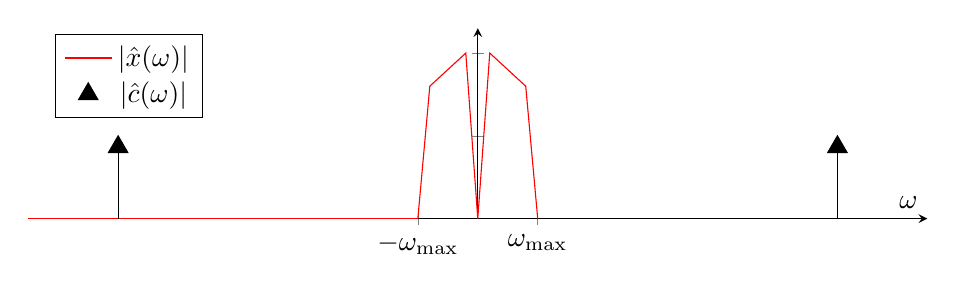
\begin{tikzpicture}
	\begin{axis}[
        width=13cm,
        height=4cm,
        ymin=0,
        ymax=2.3,
    	xmin=-7.5,
        xmax=7.5,
        xlabel={$\omega$},
%        ylabel={$\hat{x}(\omega)$},
        axis x line=center, 
        axis y line=center, 
        yticklabels={,,,},
        xtick={-1,1},
        legend pos=north west,
        xticklabels={$-\omega_{\mathrm{max}}$,$\omega_{\mathrm{max}}$}
    ]
    \addplot[mark=none,color=red] plot coordinates {(-10,0.0) (-1,0) (-0.8,2*0.8) (-0.2,2*1) (0,0) (0.2,2*1) (0.8,2*0.8) (1,0) } ;
\addplot +[dirac,color=black] coordinates {(-6,1.0) (6,1.0)};

%\addplot[mark=none,color=blue] plot coordinates {(-10,0.0) (-7,0) (-6.8,0.8) (-6.2,1) (-6,0) (-5.8,1) (-5.2,0.8) (-5,0) (5,0) (5.2,0.8) (5.8,1) (6,0) (6.2,1) (6.8,0.8) (7,0) (10,0)  } ;
\addlegendentry{$|\hat{x}(\omega)|$}
\addlegendentry{$|\hat{c}(\omega)|$}

%\addlegendentry{$|\hat{Y}(i\omega)|$}
\end{axis}
\end{tikzpicture}
\end{center}
\caption{A spectral representation of signals $x(t)$ and $c(t)$.}
\label{fig:am_spectra0}
\end{figure}
The spectrum of the signal $c(t)$ can be determined by first representing the 
signal as a sum of two complex sinusoids (using Euler's formula):
\begin{equation}
c(t) = \cos(\omega_c t) = \frac{1}{2}e^{i\omega_c t} + \frac{1}{2} e^{-i\omega_c t}\,\,.
\end{equation}
We know that the spectrum of a complex sinusoid is a frequency shifted
Dirac-delta, and hence, the Fourier transform of $c(t)$ is
\begin{equation}
\hat{c}(\omega) = \pi\delta(\omega - \omega_c) + \pi\delta(\omega + \omega_c)\,\,.
\end{equation}
We also know from the convolution theorem, that multiplying two
signals in time domain results in convolution in frequency domain:
\begin{equation}
y(t) = x(t) c(t) \xleftrightarrow{\mathcal{F}} \hat{y}(\omega) = \frac{1}{2\pi}\hat{x}(\omega) * \hat{c}(\omega)\,\,.
\end{equation}
We can now inspect what the spectrum $\hat{y}(\omega)$ looks like by
evaluating the convolution:
\begin{align}
\hat{y}(\omega) & = \frac{1}{2\pi}\int_{-\infty}^{\infty} \hat{x}(\omega') \hat{c}(\omega - \omega') d\omega' \\
  &= \frac{1}{2} \int_{-\infty}^{\infty} \hat{x}(\omega')\left[ \delta(\omega - \omega_c - \omega') + \delta(\omega + \omega_c - \omega') \right] d\omega' \\
   &= \frac{1}{2}\hat{x}(\omega-\omega_c) + \frac{1}{2}\hat{x}(\omega+\omega_c)\,\,.
\end{align}
In this convolution, the Dirac delta functions act as frequency
shifters, which shift the function $\hat{x}(\omega)$ up and down in
frequency by $\omega_c$.

Figure \ref{fig:am_spectra1} shows a plot of the spectrum of the original signal $x(t)$, and the
upconverted signal $y(t)$.
\begin{figure}
\begin{center}
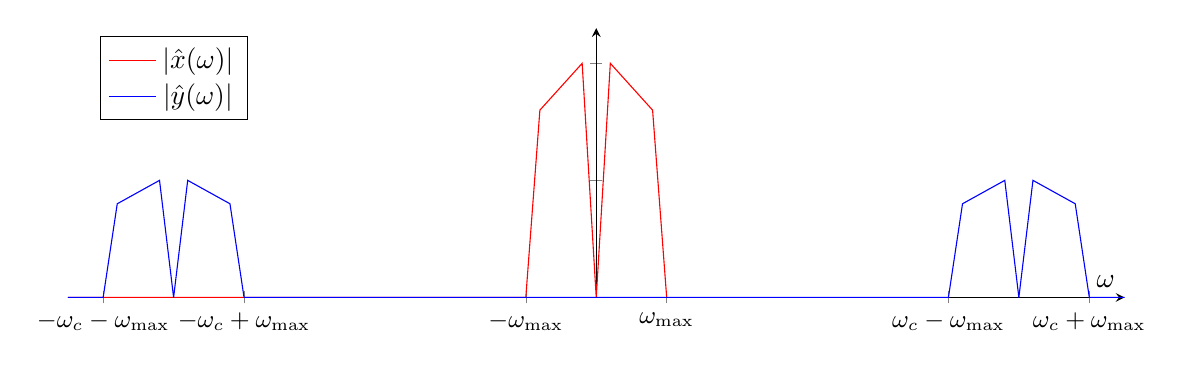
\begin{tikzpicture}
	\begin{axis}[
        width=15cm,height=5cm,ymin=0,ymax=2.3,
    	xmin=-7.5,xmax=7.5,
        xlabel={$\omega$},
%        ylabel={$\hat{Y}(i\omega)$},
        axis x line=center, 
        axis y line=center, 
        yticklabels={,,,},
        ticklabel style = {font=\small},
        xtick={-7,-5,-1,1,5,7},
                legend pos=north west,
        xticklabels={$-\omega_c-\omega_{\mathrm{max}}$,$-\omega_c+\omega_{\mathrm{max}}$,$-\omega_{\mathrm{max}}$,$\omega_{\mathrm{max}}$,$\omega_c-\omega_{\mathrm{max}}$,$ \omega_c+\omega_{\mathrm{max}}$}
    ]
    \addplot[mark=none,color=red] plot coordinates {(-10,0.0) (-1,0) (-0.8,2*0.8) (-0.2,2*1) (0,0) (0.2,2*1) (0.8,2*0.8) (1,0) } ;

\addplot[mark=none,color=blue] plot coordinates {(-10,0.0) (-7,0) (-6.8,0.8) (-6.2,1) (-6,0) (-5.8,1) (-5.2,0.8) (-5,0) (5,0) (5.2,0.8) (5.8,1) (6,0) (6.2,1) (6.8,0.8) (7,0) (10,0)  } ;

\addlegendentry{$|\hat{x}(\omega)|$}
\addlegendentry{$|\hat{y}(\omega)|$}
\end{axis}
\end{tikzpicture}
\end{center}
\caption{The spectrum of the amplitude modulated signal consists of two
copies of the spectrum of the original signal, shifted up and down by
$\omega_c$ in frequency and scaled by $\frac{1}{2}$ in amplitude.}
\label{fig:am_spectra1}
\end{figure}

\newthought{In order to reconstruct the audio signal $x(t)$ from the modulated
signal $y(t)$}, the signal is first multiplied with the carrier
signal:
\begin{equation}
w(t) = y(t)c(t)\,\,.
\end{equation}

This operation again is a frequency shift, just like in the modulation
step. We can again use the convolution theorem to
obtain the spectrum of the intermediate signal $w(t)$:

\begin{marginfigure}[-1.5cm]
\begin{center}
\begin{circuitikz}
%\path (2,0) node[above=2pt]() {$c(t)=\cos(\omega_c t)$} to[sV]node[pos=0,inner sep=0pt](b){} (2,2);

\draw (-2,0) node[](c) {$c(t)=\cos(\omega_c t)$};% to[sV]node[pos=0,inner sep=0pt](b){} (2,2);

\draw (0,-1) node[scale=0.8](bp) {};

\draw (0,-4) node[scale=0.8](out) {$v(t)$};

\draw (0,2) node[scale=0.8](buf){$y(t)=x(t)\cos(\omega_c t)$};

\draw (0.5,-1) node {$w(t)$};

\draw (-0.45,0) node(mixin0){};
\draw (0,0.45) node(mixin1){};

\draw (0,-0.45) node(mixout){};
\draw (0,-1.6) node(bpin){};
\draw (0,-2.4) node(bpout){};

%\path (0,1) to [sV,color=white,name=bp] node[pos=0,inner sep=0pt](d){} node[above left=0.8cm and 0.0cm]{LPF} (0,2);
%\draw (0,2) node(lpf);
%\path (0,0) to [sV,color=white,name=M1] node[midway,above=0.1cm]{Mixer}(0,0);
\draw (0,0) node[inner sep=0pt,color=white] (M1){};
\mixer{M1}
\draw (0,-2) node[sV](bp){};
\LPF{bp}{0}
%\draw[ar] (b)--(M1);
\draw[ar] (c)--(mixin0);
\draw[ar] (buf)--(mixin1);
\draw[ar] (mixout)--(bpin);
\draw[ar] (bpout)--(out);
\end{circuitikz}
\end{center}
\caption{Demodulation or conversion of a high frequency signal $y(t)$ into an audio signal $v(t)$.}
\label{fig:am_demod}
\end{marginfigure}

\begin{align}
\hat{w}(\omega) =& \frac{1}{2\pi} \hat{y}(\omega)*\hat{c}(\omega)\\
 =& \frac{1}{2}\hat{y}(\omega+\omega_c) + \frac{1}{2}\hat{y}(\omega-\omega_c) \\
                 =& \frac{1}{4}\left[\hat{x}(\omega+\omega_c+\omega_c) + \hat{x}(\omega-\omega_c+\omega_c)\right] \\
                 &+ \frac{1}{4}\left[\hat{x}(\omega+\omega_c-\omega_c) + \hat{x}(\omega-\omega_c-\omega_c)\right] \\
                 =& \frac{1}{4}\hat{x}(\omega - 2\omega_c)+ \frac{1}{4}\hat{x}(\omega + 2\omega_c) + \frac{1}{2}\hat{x}(\omega)\,\,.
\end{align}

There are now three copies of the spectrum $\hat{x}(\omega)$. One
centered at $\omega=0$ and two centered at twice the carrier frequency
$\omega=\pm 2\omega_c$ as shown in Figure \ref{fig:am_spectra_demod}.
\begin{figure}
\begin{center}
\begin{tikzpicture}
	\begin{axis}[width=15cm,height=5cm,ymin=0,ymax=3,
    	xmin=-11,xmax=11,
        xlabel={$\omega$},
        ylabel={$|\hat{w}(\omega)|$},
        axis x line=center, 
        axis y line=center, 
        yticklabels={,,,},
        xtick={-6,-1,1,6},
        xticklabels={$-2\omega_c$,$-\omega_{\mathrm{max}}$,$\omega_{\mathrm{max}}$,$2\omega_c$}
    ]
    \addplot[mark=none,color=blue] plot coordinates {(-10,0.0) (-1,0) (-0.8,2*0.8) (-0.2,2*1) (0,0) (0.2,2*1) (0.8,2*0.8) (1,0) } ;

\addplot[mark=none,color=blue] plot coordinates {(-10,0.0) (-7,0) (-6.8,0.8) (-6.2,1) (-6,0) (-5.8,1) (-5.2,0.8) (-5,0) (5,0) (5.2,0.8) (5.8,1) (6,0) (6.2,1) (6.8,0.8) (7,0) (10,0)  } ;


\addplot[mark=none,color=red] plot coordinates {(-10,0.0) (-2,0) (-2,2.2) (2,2.2) (2,0) (10,0) } ;

\node at (axis cs:3,1.5) [color=red]{$\mathcal{H}(\omega)$};

%\addlegendentry{$|\hat{w}(i\omega)|$}
\end{axis}
\end{tikzpicture}
\end{center}
\caption{Spectra of an AM demodulated signal.}
\label{fig:am_spectra_demod}
\end{figure}

We almost have what we need, but we need to get rid of the high
frequency components. This can be done with the help of a low-pass
filter:
\begin{equation}
\mathcal{H}(\omega) = \left\{ \begin{array}{cc}
2, & |\omega| \le \omega_{\mathrm{max}} \\
0, & \mathrm{otherwise}
\end{array}\right.\,\,.
\end{equation}
which also corrects the scale back to the original. The frequency
response of such a filter is shown in both Figure \ref{fig:am_spectra_demod} and \ref{fig:am_final_spectrum} with red. The output
signal spectrum is then:
\begin{align}
\hat{v}(\omega) &= \Hiw \hat{w}(\omega) \\
           &= \hat{x}(\omega)\,\,.
\end{align}
And therefore $v(t)=x(t)$. Multiplying with a cosine signal and
low-pass filtering has shifted the signal back to DC and allowed us to
reconstruct the original signal $x(t)$.


\begin{figure}
\begin{center}
\begin{tikzpicture}
	\begin{axis}[width=15cm,height=5cm,ymin=0,ymax=3,
    	xmin=-11,xmax=11,
        xlabel={$\omega$},
        ylabel={$\hat{v}(\omega)=\hat{x}(\omega)$},
        axis x line=center, 
        axis y line=center, 
        yticklabels={,,,},
        xtick={-1,1},
        xticklabels={$-\omega_{\mathrm{max}}$,$\omega_{\mathrm{max}}$}
    ]
    \addplot[mark=none,color=blue] plot coordinates {(-10,0.0) (-1,0) (-0.8,2*0.8) (-0.2,2*1) (0,0) (0.2,2*1) (0.8,2*0.8) (1,0) } ;

%\addplot[mark=none,color=blue] plot coordinates {(-10,0.0) (-7,0) (-6.8,0.8) (-6.2,1) (-6,0) (-5.8,1) (-5.2,0.8) (-5,0) (5,0) (5.2,0.8) (5.8,1) (6,0) (6.2,1) (6.8,0.8) (7,0) (10,0)  } ;


\addplot[mark=none,color=red] plot coordinates {(-10,0.0) (-2,0) (-2,2.2) (2,2.2) (2,0) (10,0) } ;
\node at (axis cs:3,1.5) [color=red]{$\mathcal{H}(\omega)$};

%\addlegendentry{$|\hat{W}(i\omega)|$}
\end{axis}
\end{tikzpicture}
\end{center}
\caption{The original signal spectrum $\hat{x}(\omega)$ reconstructed from the high frequency signal.}
\label{fig:am_final_spectrum}
\end{figure}
\newpage
\section{RC-circuit [Optional]}
Consider the following electrical circuit:
\begin{center}
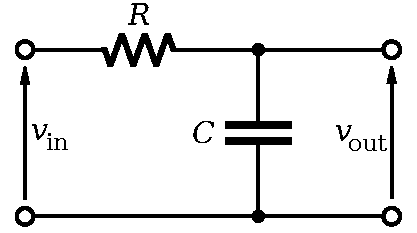
\includegraphics[width=0.5\textwidth]{Applications/figures/rc.pdf}
\end{center}
This is a very simple analogue filter implemented using a resistor and
a capacitor. This type of circuit is often used in, e.g., audio
electronics to remove high-pitched signals.

This system can be modeled as a linear time-invariant system. In this
case, $v_{\mathrm{in}}(t) = x(t)$ and $v_{\mathrm{out}}(t) =
y(t)$. This system has the following impulse response:
\begin{equation}
h(t) = \frac{1}{RC} e^{-\frac{1}{RC}t}u(t) = \alpha e^{-\alpha t} u(t)
\end{equation}
where the real valued constant $\alpha > 0$. 

In order to determine the frequency response, we evaluate the Fourier 
transform of the impulse response:
\begin{align}
\Hiw &= \int_{-\infty}^{\infty} \alpha e^{-\alpha t} u(t) e^{-i\omega t}dt \\
     &= \alpha \int_{0}^{\infty} e^{-(\alpha+i\omega) t} dt \\
     &= \alpha \left. \frac{e^{-(\alpha+i\omega)t}}{-(\alpha+i\omega)}\right\rvert_{t=0}^{\infty} \\
     &= \frac{\alpha}{\alpha + i\omega}\,\,.
\end{align}
In order to find the magnitude response, we'll need to establish that
\begin{equation}
  \mathcal{H}^*(\omega) = \frac{\alpha}{\alpha - i\omega}\,\,,
\end{equation}
which is relatively easy to show\footnote{For example using: \begin{equation*}\frac{\alpha}{\alpha + i \omega} = \frac{\alpha(\alpha - i\omega)}{\alpha^2 + \omega^2} = \frac{\alpha^2}{\alpha^2 + \omega^2} - i\frac{\alpha\omega}{\alpha^2 + \omega^2}\end{equation*}}.

The magnitude response is then:
\begin{align}
|\Hiw| &= \sqrt{\Hiw\mathcal{H}^*(\omega)}\\
       &= \frac{\alpha}{\sqrt{\alpha^2 + \omega^2}}\,\,.
\end{align}
The phase response is\footnote{recall that $\tan^{-1}(-x) = -\tan^{-1}(x)$}:
\begin{align}
\angle \Hiw &= \tan^{-1}{\frac{\mathrm{Im}(\Hiw)}{\mathrm{Re}(\Hiw)}} \\
            &= - \tan^{-1}{\frac{\omega}{\alpha}}\,\,.
\end{align}
The magnitude and phase responses are plotted below:
\begin{center}
\begin{minipage}{.49\textwidth}
\begin{tikzpicture}
	\begin{axis}[domain=(-150):(150),samples=200,ymax=1.2,
        xlabel={$\omega$},
        ylabel={$|\Hiw|$},
        axis x line=center, 
        axis y line=middle,
        ytick={0.707,1.0},
        yticklabels={$\frac{1}{\sqrt{2}}$,$1$},
        xtick={-40,40},
        xticklabels={$-\alpha$,$\alpha$}
    ]
        \addplot [dashed,black] coordinates { (-40,0.0) (-40,0.707) };
        \addplot [dashed,black] coordinates { (40,0.0) (40,0.707) };
        \addplot [dashed,black] coordinates { (-40,0.707) (40,0.707) };
        
	\addplot[blue] {40/sqrt(x*x+40*40)};
    \end{axis}
\end{tikzpicture}
\end{minipage}
\begin{minipage}{.49\textwidth}
\begin{tikzpicture}
	\begin{axis}[domain=(-150):(150),samples=200,ymin=-100,ymax=100,
        xlabel={$\omega$},
        ylabel={$\angle \Hiw$},
        axis x line=center, 
        axis y line=middle, 
        ytick={-90,-45,45,90},
        yticklabels={$-\frac{\pi}{2}$,$-\frac{\pi}{4}$,$\frac{\pi}{4}$,$\frac{\pi}{2}$},    
        xtick={-40,40},
        xticklabels={$-\alpha$,$\alpha$}    
    ]
    \addplot[blue] {-atan(x/40.0)};
    \addplot[dashed,blue] {-180*x/40.0/3.14};
\addplot [dashed,black] coordinates { (-40,0.0) (-40,45) };
        \addplot [dashed,black] coordinates { (40,0.0) (40,-45) };
        \addplot [dashed,black] coordinates { (-40,45) (0,45) };
        \addplot [dashed,black] coordinates { (40,-45) (0,-45) };

\end{axis}
\end{tikzpicture}
\end{minipage}
\end{center}
Note that the ``half-power'' point, where $|\Hiw|^2=\frac{1}{2}$
corresponds to $\omega = \pm \alpha$. This half power width of a
filter is often referred to as the full width half maximum (FWHM). At
this ``half-power'' point, the phase is $- \tan^{-1}(\pm 1)
= \mp \frac{\pi}{4}$. For our example filter, the output power has
dropped to half when the frequency is:
\begin{equation}
\omega = 2\pi f = \frac{1}{RC}
\end{equation}
or 
\begin{equation}
f = \frac{1}{2\pi RC}\,\,.
\end{equation}
For example, if $R=1$ k$\Omega$ and $C=100$ pF, the cutoff frequency
of the filter is 1.6 MHz.

When looking at the Taylor series expansion of the phase around zero,
recalling that
\begin{equation}
\frac{d}{d\omega}\tan^{-1}(-\omega/\alpha) = \frac{\alpha}{\omega^2 + \alpha^2}\,\,,
\end{equation}
we get
\begin{equation}
\angle\Hiw \approx -\frac{1}{\alpha}\omega = -RC \omega\,\,.
\end{equation}
This is shown as a dashed blue line in the figure above. 

If we compare this with the equation for delay of a sinusoid
$x(t)=Ae^{i\omega t}$, which we can derive from
\begin{equation}
x(t-t_0) = Ae^{i\omega(t-t_0)} = Ae^{i\omega t} e^{-i\omega t_0} = Ae^{i\omega t} e^{i\varphi} 
\end{equation}
to be $-\omega t_0 = -RC\omega$, we see that the filter corresponds to
approximately a $t_0 = RC$ second time delay. This approximation is
valid for low values of $|\omega| < \frac{1}{2}\alpha$. In the case of
$R=1$ k$\Omega$ and $C=100$ pF, the time delay is approximately: 0.1
$\mu$s.




\fi

\ifSpDT
\chapter{Discrete-time Signals}
\begin{marginfigure}
  \begin{center}
    \begin{tikzpicture}
      \begin{axis}[domain=-2*3.1415:2*3.1415,
        width=7cm,height=5cm,ymin=-2.5,xmin=0,ymax=2.5,xmax=6,
        ytick={-1,1},
        yticklabels={,,},
        xticklabels={,,},
        ylabel={$x(t),{\color{blue}x[n]}$},
        xlabel=$t$, axis lines = center]
        \addplot+[ycomb,samples=15] {-0.5+sin(deg(x))+0.5*sin(2*deg(0.5*x)-0.0)+0.7*sin(3*deg(x)-0.6)+0.3*sin(4*deg(x)+1.6)};
        \addplot[samples=200]{-0.5+sin(deg(x))+0.5*sin(2*deg(0.5*x)-0.0)+0.7*sin(3*deg(x)-0.6)+0.3*sin(4*deg(x)+1.6)};
        \node at (axis cs:0.9+0.45,1.1) [above, font={\footnotesize}]{$T_s$};
        \addplot [dimen,black]plot coordinates {(0.9,1.1) (2.0*0.9,1.1)};
      \end{axis}\
    \end{tikzpicture}
  \end{center}
  \caption{A continuous-time signal $x(t)$, and a discrete-time signal
    $x[n]$. Sample-spacing $T_s$ is related to sample-rate as follows:
    $T_s = 1/f_s$.}

\end{marginfigure}
In this chapter, we introduce discrete-time signals. These are the
type of signals that are used for digital signal processing. We'll
cover the following topics:
\begin{itemize}
  \item Discretization
  \item Aliasing
  \item Oversampling and undersampling
  \item Reconstruction
  \item Shannon-Nyquist sampling theorem
\end{itemize}
We'll need to know about complex sinusoidal signals and the frequency
domain representation of signals (the Fourier transform).

\section{Sampling}
\begin{marginfigure}
  \tikzstyle{int}=[draw, minimum size=2em]
  \tikzstyle{init} = [pin edge={to-,thin,black}]
  \begin{center}
    %  \resizebox{\columnwidth}{!}{%
    \begin{tikzpicture}[every text node part/.style={align=center},node distance=3cm,auto,>=latex']
      \node [int] (a) {C-to-D \\ $T_s$};
      \node (b) [left of=a,node distance=2cm, coordinate] {a};
      %    \node (c) [below=a,node distance=3cm] {a};

      %\node [int, pin={[init]above:$p_0$}] (c) [right of=a] {$\frac{1}{s}$};
      \node [coordinate] (end) [right of=a, node distance=3cm]{};
      \path[->] (b) edge node {$x(t)$} (a);
      %\path[->] (a) edge node {$v$} (c);
      \draw[->] (a) edge node {$x[n]=x(nT_s)$} (end) ;
    \end{tikzpicture}
    % }
  \end{center}
  \caption{An ideal continuous-time to Discrete-time (C-to-D) converter.}
\end{marginfigure}


A continuous-time signal can be converted into a discrete-time signal
by sampling it. This can be idealized as a system that performs the following operation:
\begin{equation}
  \boxed{
    x[n] = x(n T_s)
  }\,\,.
\end{equation}
In this process, a continuous function $x(t) \in \mathbb{C}$ is converted into an ordered 
sequence of numbers $x[n] \in \mathbb{C}$, where $n\in\mathbb{Z}$ indicates the order of the numbers.

The reason why we consider complex-valued signals in addition to real-valued signals is 
that there are many applications where the signals are naturally complex-valued. 
Radio signal processing is one example.

The \index{sample-spacing}{sample-spacing} $T_s$ determines how densely samples of the 
continuous-time signal are taken. Sample-spacing is related with the \index{sample-rate}{sample-rate} 
or \index{sampling-rate}{sampling-rate} $f_s$ as follows:
\begin{equation}
  \boxed{
    f_s = \frac{1}{T_s}
  }\,\,.
\end{equation}
Sample-rate typically is given in units of samples per second or hertz, but other units are also used in various applications.
For example, the resolution of a digital image is often given in units of dots per inch (DPI).

\if 0 You can think of sampling as a convolution operation between a
  time-shifted unit impulse $\delta(t-nT_s)$ and the continuous-time
  signal $x(t)$:
  \begin{align}
    x[n] & = \int_{-\infty}^{\infty} x(\tau) \delta(n T_s - \tau)  d\tau \\
         & = x(n T_s)\,\,.
  \end{align}
\fi

\subsection{Sampling a complex sinusoidal signal}
In order to understand sampling, you need to understand how sampling affects a complex sinusoidal signal:
\begin{equation}
  x(t)=A e^{i\phi} e^{i\omega_0 t}\,\,.
\end{equation}
Because we can use the Fourier transform to represent signals as a superposition of complex 
sinusoidal signals, knowledge of what happens to a fixed frequency signal will tell us how 
discretization affect signals more generally.

\begin{marginfigure}
  \begin{center}
    \begin{tikzpicture}
      \begin{axis}[width=7cm,height=6cm,ymin=0,xmin=-3,ymax=1.5,xmax=3,  yticklabels={,,},
          xtick={1.0},
          ylabel={$\hat{x}(\omega)$},
          xticklabels={$\omega_0$},
          xlabel=$\omega$, axis lines = center]

        \addplot + [ycomb] plot coordinates {(1,1)};
        \node at (axis cs:1,1.1) [above, font={\footnotesize}]{$Ae^{i\phi}$};
      \end{axis}
    \end{tikzpicture}
  \end{center}
\end{marginfigure}

So what happens to a complex sinusoidal signal when we sample it?
\begin{align}
  x[n] & =x(nT_s)                                \\
       & =A e^{i\phi} e^{i\omega_0 n T_s }       \\
       & =A e^{i\phi} e^{i\hat{\omega}_0 n}\,\,.
\end{align}
What happens is that we get a discrete-time complex sinusoidal signal. This signal has a special type of frequency:
\begin{equation}
  \boxed{
    \hat{\omega}_0 = \omega_0 T_s
  }\,\,.
\end{equation}

The angular frequency $\hat{\omega}_0$ is called a \emph{\index{discrete-time angular frequency}{discrete-time angular frequency}}.
It indicates how many \emph{\index{radians per sample}{radians per sample}} the phase of 
the complex sinusoidal signal advances. With a discrete-time signal, time is only 
implied from the sample spacing that was used to discretize the signal, which is 
why no time unit is attached to $\hat{\omega}_0$. There's a hat on $\hat{\omega}_0$ 
to signify that this is not the same kind of frequency as the continuous-time angular 
frequency $\omega$, which has units of radians per second.

Figure \ref{fig:rotating_dt_phasor} shows an example of how the values of the discrete-time complex 
sinusoidal signal behave with increasing sample index, obtaining values on a circle of 
radius $A$ in the complex plane. The amount of angle per sample that the signal advances for
each sample on the circle is given by the discrete-time angular frequency $\hat{\omega}_0$.

\begin{marginfigure}
  \begin{center}
    \begin{tikzpicture}
      \pgfmathsetmacro{\PHI}{38}
      \pgfmathsetmacro{\OM}{64}
      \begin{axis}[axis equal, disabledatascaling,
          ymin=-1.5,xmin=-1.5,ymax=1.5,xmax=1.5, ticks=none,
          xlabel=$\mathrm{Re}$, ylabel=$\mathrm{Im}$, axis lines = center,
          width=7cm, height=7cm]
        % unit circle
        \addplot [gray,domain=0:2*pi,samples=50]({cos(deg(x))},{sin(deg(x))});
        % first sample
        \addplot [black, mark = *] coordinates {( {cos(\PHI)}, {sin(\PHI)} )} {};
        \addplot [black] coordinates { (0,0) ( {cos(\PHI)}, {sin(\PHI)} ) };

        % second sample
        \addplot [black, mark = *] coordinates {( {cos(\OM+\PHI)}, {sin(\OM+\PHI)} )} {};
        \addplot [black] coordinates { (0,0) ( {cos(\OM+\PHI)}, {sin(\OM+\PHI)} ) };

        % third sample
        \addplot [black, mark = *] coordinates {( {cos(2*\OM+\PHI)}, {sin(2*\OM+\PHI)} )} {};
        \addplot [black] coordinates { (0,0) ( {cos(2*\OM+\PHI)}, {sin(2*\OM+\PHI)} ) };

        % third sample
        \addplot [black, mark = *] coordinates {( {cos(3*\OM+\PHI)}, {sin(3*\OM+\PHI)} )} {};
        \addplot [black] coordinates { (0,0) ( {cos(3*\OM+\PHI)}, {sin(3*\OM+\PHI)} ) };

        \node at (axis cs:{1.2*cos(\PHI)},{1.2*sin(\PHI)}) {$x[0]$};
        \node at (axis cs:{1.2*cos(\OM+\PHI)},{1.2*sin(1*\OM+\PHI)}) {$x[1]$};
        \node at (axis cs:{1.2*cos(2*\OM+\PHI)},{1.2*sin(2*\OM+\PHI)}) {$x[2]$};
        \node at (axis cs:{1.2*cos(3*\OM+\PHI8)},{1.2*sin(3*\OM+\PHI)}) {$x[3]$};


        \addplot [red,domain=0:(pi*\PHI/180),samples=50]({0.3*cos(deg(x))},{0.3*sin(deg(x))});
        \node at (axis cs:{0.5*cos(\PHI/2.0)},{0.4*sin(\PHI/2.0)}) {$\phi$};

        \addplot [blue,domain=(pi*\PHI/180):(pi*(\PHI+\OM)/180),samples=50]({0.3*cos(deg(x))},{0.3*sin(deg(x))});
        \node at (axis cs:{0.5*cos((\PHI+\PHI+\OM)/2)},{0.4*sin((\PHI+\PHI+\OM)/2)}) {$\hat{\omega}_0$};

        \addplot [blue,domain=(pi*(\PHI+\OM)/180):(pi*(\PHI+2*\OM)/180),samples=50]({0.3*cos(deg(x))},{0.3*sin(deg(x))});
        \node at (axis cs:{0.5*cos((\PHI+\OM + \PHI+2*\OM)/2)},{0.4*sin((\PHI+\OM + \PHI+2*\OM)/2)}) {$\hat{\omega}_0$};

        \addplot [blue,domain=(pi*(\PHI+2*\OM)/180):(pi*(\PHI+3*\OM)/180),samples=50]({0.3*cos(deg(x))},{0.3*sin(deg(x))});
        \node at (axis cs:{0.5*cos((\PHI+2*\OM + \PHI+3*\OM)/2)},{0.4*sin((\PHI+2*\OM + \PHI+3*\OM)/2)}) {$\hat{\omega}_0$};

      \end{axis}
    \end{tikzpicture}
  \end{center}
  \caption{A discretized complex sinusoidal signal $x[n] = A e^{i\phi}e^{i\hat{\omega}_0n}$ 
  with phase increments of $\hat{\omega}_0$ radians per sample. The initial phase for sample $n=0$ is given by $\phi$.}
  \label{fig:rotating_dt_phasor}
\end{marginfigure}

\subsection{Frequency aliases}
What happens if $\hat{\omega}$ gets larger? What if it is so large that the phasor rotates 
around the circle on the complex plane one or more times every sample? 
This phenomenon is called aliasing.

Here's a more formal way of defining aliasing. The complex sinusoidal
signal $e^{i\hat{\omega}_0 n}$ is not unique. There are infinitely
many possible frequency increments that result in the same signal:
\begin{align}
  x[n] & =Ae^{i\phi} e^{i(\hat{\omega}_0 + 2\pi k) n} \\
       & =Ae^{i\phi} e^{i \hat{\omega}_0  n}
\end{align}
where $k\in\mathbb{Z}$. What this means is that we can select any one
of the discrete-time angular frequencies:
\begin{equation}
  \boxed{
    \hat{\omega}_k = \hat{\omega}_0 + 2\pi k
  }\,\,.
\end{equation}
and our discrete-time complex sinusoidal signal will be
identical. There is no way of telling just from the signal itself what
the true discrete-time angular frequency is. Frequencies
$\hat{\omega}_k$ are called \emph{\index{aliases}{aliases}}. There are
infinitely many such aliases.

\begin{marginfigure}[5cm]
  \begin{center}
    \begin{tikzpicture}
      \begin{axis}[
          width=7cm,
          height=6cm,
          ymin=0,
          xmin=-4,
          ymax=1.2,
          xmax=4,
          yticklabels={,,},
          xtick={-3.6,-1.6, .4, 2.4},
          xticklabels={$f_0-2 f_s $,$f_0- f_s$,$f_0$,$f_0+f_s$},
          xlabel=$f$,
          ylabel=$\hat{x}(f)$,
          axis lines = center]
        \addplot+[ycomb] plot coordinates {((-3.6,1) (-1.6,1) (0.4,1) (2.4,1)};
      \end{axis}
    \end{tikzpicture}
  \end{center}
  \caption{Each one of these signals $Ae^{i\phi}e^{i2\pi (f_0 + k f_s)t}$
  would result in the same discrete-time complex sinusoidal signal
  when discretized with sample-rate $f_s$. Note that we're showing the
  spectrum with continuous-time frequency in units of hertz (cycles
  per second) instead of radians per second.}
\end{marginfigure}

What continuous-time frequencies do these aliases correspond to? We
can work this out by looking at the continuous-time signal of
frequency $\omega_0$:
\begin{equation}
  x(t) = A e^{i\phi} e^{i\omega_0 t}\,\,.
\end{equation}
When discretized, each of the following signals are identical:
\begin{align}
  x[n] & =A e^{i\phi} e^{i \omega_0 T_s n }                \\
       & = A e^{i\phi} e^{i(\omega_0 T_s + 2\pi k) n }     \\
       & = A e^{i\phi} e^{i(\omega_0 + 2\pi k/T_s) T_s n } \\
       & = A e^{i\phi} e^{i(\omega_0 + 2\pi k f_s) T_s n } \\
       & = A e^{i\phi} e^{i \omega_k T_s n } \,\,.
\end{align}
We've used the relationship between sample-rate $f_s=1/T_s$ and sample
spacing here. The aliases map to continuous-time angular frequency as
follows:
\begin{equation}
  \boxed{
    \omega_k = \omega_0 + 2\pi k f_s
  }\,\,
\end{equation}

Any one of these continuous-time angular frequencies $\omega_k$ would
result in an identical discrete-time complex sinusoidal signal when
discretized with sample-rate $f_s$. Dividing by
$2\pi$, we get the aliasing behavior in units of hertz (samples per
second)\footnote{remember that angular frequency (radians per second)
  and frequency (cycles per second) are related as follows $\omega = 2\pi
    f$.}:
\begin{equation}
  \boxed{
    f_k = f_0 + k f_s
  }\,\,.
\end{equation}
The phenomena of aliasing is problematic. We cannot uniquely distinguish
a discrete-time complex sinusoidal signal $x[n]=Ae^{i\hat{\omega}n}$
which continuous-time signal it corresponds to. Conversely,
there are infinitely many continuous-time sinusoidal signals
$x(t)=Ae^{i\omega t}$ that will result in the same discrete-time
signal. In order to rule out the wrong solutions, we need a priori
information about the spectral occupancy of the continuous-time
signal.

\begin{marginfigure}
  \begin{center}
    \begin{tikzpicture}
      \begin{axis}[domain=-6:6,
          width=7cm,height=6cm,ymin=-1.2,xmin=-4,ymax=1.4,xmax=4,
          ytick={-1,1},
          yticklabels={$-A$, $A$},
          xlabel=$t$, axis lines = center]
        \addplot+[ycomb,samples=15,color=blue]{cos(deg(2.0*3.1415*1.35*x+3.14/4))};
        \addplot+[ycomb,samples=15,color=red]{sin(deg(2.0*3.1415*1.35*x+3.14/4))};

        \addplot[samples=400,blue]{cos(deg(2.0*3.1415*1.35*x+3.14/4))};
        \addplot[samples=400,red]{sin(deg(2.0*3.1415*1.35*x+3.14/4))};
        %            \addplot[samples=400,color=red]{cos(deg(2.0*3.1415*0.18333333333333335*x+3.14/4))};
        %           \addplot[samples=400,color=green]{cos(deg(2.0*3.1415*0.9833333333333334*x-3.14/4))};


        \node  at (axis cs:0.9+0.45,1.1) [above, font={\footnotesize}]{$T_s$};
        \addplot [dimen,black]plot coordinates {(0.9,1.1) (2.0*0.9,1.1)};
      \end{axis}

    \end{tikzpicture}
    \begin{tikzpicture}
      \begin{axis}[domain=-6:6,
          width=7cm,height=6cm,ymin=-1.2,xmin=-4,ymax=1.4,xmax=4,
          ytick={-1,1},
          yticklabels={$-A$, $A$},
          xlabel=$t$, axis lines = center]
        %            \addplot[samples=400,blue]{cos(deg(2.0*3.1415*1.35*x+3.14/4))};
        \addplot+[ycomb,samples=15,color=blue]{cos(deg(2.0*3.1415*0.18333333333333335*x+3.14/4))};
        \addplot+[ycomb,samples=15,color=red]{sin(deg(2.0*3.1415*0.18333333333333335*x+3.14/4))};
        \addplot[samples=400,color=blue]{cos(deg(2.0*3.1415*0.18333333333333335*x+3.14/4))};
        \addplot[samples=400,color=red]{sin(deg(2.0*3.1415*0.18333333333333335*x+3.14/4))};
        %            \addplot[samples=400,color=green]{cos(deg(2.0*3.1415*0.9833333333333334*x-3.14/4))};


        \node  at (axis cs:0.9+0.45,1.1) [above, font={\footnotesize}]{$T_s$};
        \addplot [dimen,black]plot coordinates {(0.9,1.1) (2.0*0.9,1.1)};
        %\addplot[color=black] plot coordinates {(0.9,1.1) (2.0*0.9,1.1)};
      \end{axis}
    \end{tikzpicture}
  \end{center}
  \caption{Two different complex sinusoidal signals that result in the same discrete-time signal.}
\end{marginfigure}

Solving the problem of aliasing, by ensuring that there is a uniquely one-to-one mapping 
between continuous-time and discrete-time frequencies for all the spectral components 
of a signal, leads to the Shannon-Nyquist sampling theorem, which is introduced at the end of this chapter.

\subsection{Real-valued signals}
The concept of aliasing of complex sinusoidal signals allows us to inspect aliasing of 
real-valued sinusoidal signals, which come in pairs of positive and negative frequency 
spectral components. Understanding aliasing for real-valued signals is slightly more 
complicated than understanding complex-valued signals, because of the symmetric 
pairing of the positive and negative frequency components.

The Fourier transform of a real-valued signal $x(t)\in\mathbb{R}$ is conjugate symmetric
\begin{equation}
  \hat{x}(\omega) = \hat{x}^*(-\omega)\,\,.
\end{equation}
This means that real-valued signals are composed of conjugate
symmetric pairs of positive and negative frequency spectral
components:
\begin{equation}
  A \cos(\omega t + \phi) = \frac{A}{2}(e^{i\phi}e^{i\omega t} + e^{-i\phi}e^{-i\omega t})\,\,.
\end{equation}
In order to understand how aliasing affects real-valued signals, we
need to investigate how pairs of positive and negative frequency spectral components are affected.
\begin{marginfigure}
  \begin{center}
    \begin{tikzpicture}
      \begin{axis}[width=7cm,height=6cm,ymin=0,xmin=-2,ymax=1.5,xmax=2,  yticklabels={,,},
          xtick={-1, 1.0},
          xticklabels={$-\omega_0$,$\omega_0$},
          ylabel=$\hat{x}(\omega)$,
          xlabel=$\omega$,
          axis lines = center]

        \addplot+[ycomb] plot coordinates {(1,1)};
        \addplot+[ycomb] plot coordinates {(-1,1)};

        \node at (axis cs:1,1.1) [above, font={\footnotesize}]{$\frac{A}{2}e^{i\phi}$};
        \node at (axis cs:-1,1.1) [above, font={\footnotesize}]{$\frac{A}{2}e^{-i\phi}$};
      \end{axis}
    \end{tikzpicture}
  \end{center}
  \caption{A real-valued signal consists of a positive and negative frequency spectral component, 
  which are conjugate symmetric.}
\end{marginfigure}
A conjugate symmetric pairing of positive and negative frequencies means that there is no 
distinction between a positive and a negative frequency signal\footnote{For complex 
sinusoidal signals $e^{-i \omega t}$ and $e^{i \omega t}$ are two unique signals.}.
For example, let's say we have a signal with angular frequency $\omega = -0.1$:
\begin{equation}
  A \cos(-0.1 t + \phi) = \frac{A}{2}(e^{i\phi}e^{-i0.1  t} + e^{-i\phi}e^{i0.1 t})\,\,.
\end{equation}
This is the same thing as a cosine signal with frequency $0.1$, but a sign flipped phase:
\begin{align}
  \frac{A}{2}(e^{-i\phi}e^{i 0.1 t} + e^{i\phi}e^{-i 0.1 t}) & = A \cos(0.1 t - \phi)       \\
                                                             & = A \cos(-0.1 t + \phi)\,\,.
\end{align}
This means that you can always represent a real-valued sinusoidal signal using only 
positive valued frequencies, but it does not apply for complex-valued signals.

In the case of real-valued signals, the frequency alias corresponding to a negative 
frequency is called a \emph{\index{folded alias}{folded alias}}. For complex sinusoidal 
signals, a folded alias does not exist, as positive and negative frequency 
components are not necessarily paired.

\subsection{Example: Sinusoidal signal with $f_0=1$ Hz and $f_s=10$ Hz}
\begin{marginfigure}
  \begin{center}
    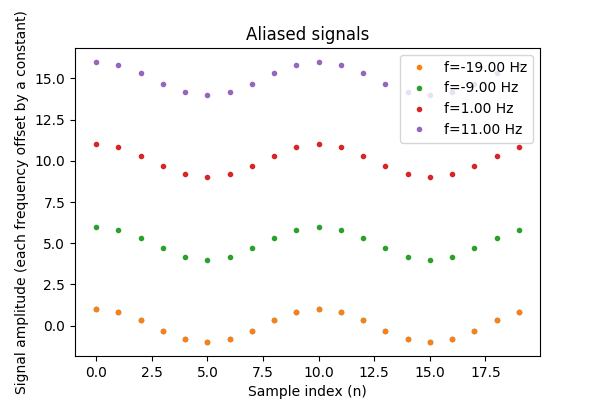
\includegraphics[width=\textwidth]{code/014_sampling/aliased_signals.png}
  \end{center}
  \caption{Example of signal aliasing for $f_0\in \{-19,-9,1,11,21\}$
    Hz and $f_s=10$ Hz. All signals alias identically. Python code:
    \texttt{014\_sampling/aliasing\_example.py}.}
\end{marginfigure}

Consider the following sinusoidal signal with a frequency of $f_0 =1$ Hz and phase $\phi$:
\begin{align}
  x(t) & =A\cos(2\pi f_0 t + \phi)  \\
  x(t) & =A\cos(2\pi t + \phi)\,\,.
\end{align}
When discretized with a sample-rate $f_s=10$ Hz or $T_s=1/f_s = 0.1$ s this becomes:
\begin{align}
  x[n] & =x(nT_s)                     \\
       & =A\cos(2\pi n T_s + \phi),   \\
       & =A\cos(0.2\pi n + \phi)\,\,.
\end{align}
The discrete-time angular frequency is $\hat{\omega}_0 = 0.2\pi$. 
For any $k\in\mathbb{Z}$ this signal is identical to:
\begin{align}
  x[n] & =A\cos([0.2\pi + 2\pi k] n + \phi)\,\,.
\end{align}
In discrete-time angular frequencies (radians per sample), the aliases are:
\begin{align}
  \hat{\omega}_k & = (0.2\pi+2\pi k)                                   \\
                 & =\ldots,-3.8\pi,-1.8\pi,0.2\pi,2.2\pi,4.2\pi,\ldots
\end{align}
In continuous-time frequency (Hz), the aliases would be:
\begin{align}
  f_k & =f_0 + f_s k                     \\
      & =\ldots,-19,-9,1,11,21,31,\ldots
\end{align}
In other words, a discretized cosine signal produced from any of the frequencies $f_k$ 
would be identical to a 1 Hz signal, when using 10 Hz sample rate. The negative solutions 
are called folded aliases, which can be interpreted as cosine signals with positive 
frequencies $9,19,\cdots$ but with a sign flipped phase.

\begin{figure}
  \begin{center}
    \begin{tikzpicture}
      \begin{axis}[
          domain=-6:6,
          width=12cm,
          height=6cm,
          ymin=-1.2,
          xmin=-4,
          ymax=1.4,
          xmax=4,
          ytick={-1,1},
          yticklabels={$-A$, $A$},
          xlabel=$t$,
          axis lines = center]
        \addplot[samples=400,blue]{cos(deg(2.0*3.1415*1.35*x+3.14/4))};
        \addplot+[ycomb,samples=15,color=red]{cos(deg(2.0*3.1415*1.35*x+3.14/4))};
        \addplot[samples=400,color=red]{cos(deg(2.0*3.1415*0.18333333333333335*x+3.14/4))};
        \addplot[samples=400,color=green]{cos(deg(2.0*3.1415*0.9833333333333334*x-3.14/4))};

        \node at (axis cs:0.9+0.45,1.1) [above, font={\footnotesize}]{$T_s$};
        \addplot[dimen,color=black] plot coordinates {(0.9,1.1) (2.0*0.9,1.1)};
      \end{axis}
    \end{tikzpicture}
  \end{center}
  \caption{The following figure illustrates what the continuous-time and discrete-time signals 
  look like. They are all identical in discrete-time, because the continuous-time signals 
  intersect at the sampling points. The red line shows $\omega_0 = 0.2\pi f_s$ (1 Hz), 
  the green line shows $\omega_1 = -1.8\pi f_s$ (-9 Hz), and the blue line shows $\omega_2=2.2\pi f_s$ (11 Hz).
  One can also see the phase-flip on the negative frequency folded alias, shown in green.
  The blue and red continuous-time signals are both sampled at identical phases, but the green not.}
\end{figure}

Figure \ref{fig:dt_spec_ex} shows part of the discrete-frequency
spectrum where there are three aliases of the cosine signal. There are infinitely many aliases, but only three are shown here.
It is customary to call the region of the spectrum where $|\hat{\omega}| < \pi$ or $|f| < f_s/2$, the \emph{principal spectrum}.
This region of the spectrums contains the smallest discrete-time angular frequency aliases.
\begin{figure}
  \begin{center}
    \begin{tikzpicture}
      \begin{axis}[width=12cm,height=6cm,ymin=0,xmin=-4,ymax=1.5,xmax=4,  yticklabels={,,},
          xtick={-2,-1,1,2},
          xticklabels={$-2\pi$,$-\pi$,$\pi$,$2\pi$},
          xlabel=$\hat{\omega}$, axis lines = center]

        \addplot[ycomb,color=blue,mark=*,mark color=blue] plot coordinates {(2.2,1)};
        \addplot[ycomb,color=green,mark=*,mark color=green] plot coordinates { (1.8,1)};
        \addplot[ycomb,color=red,mark=*,mark color=red] plot coordinates { (0.2,1)};

        \addplot[ycomb,color=blue,mark=x,mark color=blue] plot coordinates {(-2.2,1)};

        \addplot[ycomb,color=green,mark=x,mark color=green] plot coordinates {(-1.8,1)};

        \addplot[ycomb,color=red,mark=x,mark color=red] plot coordinates {(-0.2,1)};

        \node at (axis cs:0.2,1.1) [below, rotate=90, font={\footnotesize}]{Alias};
        \node at (axis cs:-0.2,1.1) [above, rotate=90, font={\footnotesize}]{Alias};
        \node at (axis cs:1.8,1.1) [below, rotate=90, font={\footnotesize}]{Folded Alias};
        \node at (axis cs:-1.8,1.1) [above, rotate=90, font={\footnotesize}]{Folded Alias};

        \node at (axis cs:2.2,1.1) [below, rotate=90, font={\footnotesize}]{Alias};
        \node at (axis cs:-2.2,1.1) [above, rotate=90, font={\footnotesize}]{Alias};

        \draw [gray, thick] (axis cs:-1,0.0) rectangle (axis cs:1,1.4);
      \end{axis}
      \begin{axis}[
          width=12cm,
          height=6cm,
          ymin=0,
          xmin=-4,
          ymax=1.5,
          xmax=4,
          yticklabels={,,},
          xlabel={},
          xtick={-2,-1,1,2},
          xticklabels={$-f_s$,$-\frac{f_s}{2}$,$\frac{f_s}{2}$,$f_s$},
          axis x line*=top]

      \end{axis}
    \end{tikzpicture}
  \end{center}
  \caption{Spectral aliases of the components plotted as a function of
    discrete-time angular frequency $\hat{\omega}$ (radians per
    sample). The pairing of positive and negative frequencies indicates
    that this signal is real-valued, and that the $\hat{\omega}_{-1} =
      -1.8\pi$ alias corresponds to a cosine signal with a positive
    discrete-time angular frequency of $1.8\pi$ and a flipped
    phase. Frequency in units of hertz is shown on the top axis.}
  \label{fig:dt_spec_ex}
\end{figure}

How could we be able to determine which one of the frequencies $f_k$ is the true sinusoidal 
frequency component represented by the discrete-time signal? We can only do this if we know 
that the continuous-time frequencies of the spectral components of the signal lie within a certain range.

For example, if we knew that there are no spectral components with frequencies higher than 5 
Hz present in the continuous-time signal ($|f| < 5$) Hz, then we could determine that the discrete-time 
signal is due to a 1 Hz continuous-time signal, because this is the only possible mapping between a 
discrete-time frequency and a continuous-time frequency.

\subsection{Principal spectrum}
The \emph{\index{principal spectrum}{principal spectrum}} (also called normalized angular frequency) 
is the range of discrete-time angular frequencies between:
\begin{equation}
  \boxed{-\pi < \hat{\omega} < \pi}\,\,.
\end{equation}
It is the region for the lowest frequency discrete-time angular frequency representation for 
discrete-time spectral components that the signal consists of. 
Unaliased continuous-time frequencies between
\begin{equation}
  -f_s/2 < f < f_s/2
\end{equation}
in units of hertz are mapped to this range of discrete-time angular frequencies.

By finding a suitable value for $k$, it is possible to find an alias of any discrete-time angular frequency $\hat{\omega}$,
which lands in the range $-\pi< \hat{\omega}+2\pi k < \pi$. This is called the \emph{\index{principal alias}{principal alias}}.
Every spectral component of a signal has an alias in the principal spectrum.

\newthought{For example}, consider a signal of frequency $f=123$ Hz:
\begin{equation}
  x(t) =\cos( 2\pi f t) = \frac{1}{2}(e^{i 2\pi f t}+e^{-i 2\pi f t})\,\,,
\end{equation}
which is sampled using a sample-rate of $f_s=100$. The discrete-time angular frequency is 
$\hat{\omega} = \pm 2\pi \cdot 123 \cdot\frac{1}{100} = \pm 2.46\pi$. 
This is outside the principal spectrum. If we shift this by $\mp 2\pi$, we obtain principal aliases:
$\hat{\omega} = \pm 0.46 \pi$.

\subsection{Folding}
Figure \ref{fig:ti_folding} shows an illustration by Texas Instruments, 
which nicely describes the concept of folding of spectral components.

\begin{marginfigure}[-4cm]
  \begin{center}
    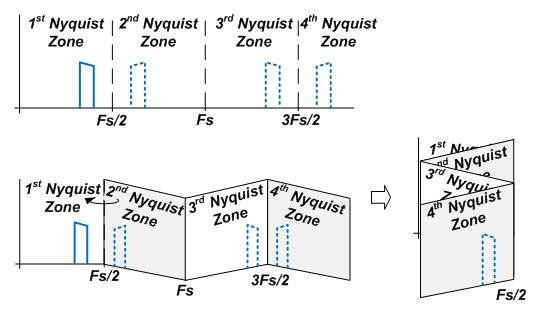
\includegraphics[width=\textwidth]{ch09/figures/folding.JPG}
  \end{center}
  \caption{Folding.}
  \label{fig:ti_folding}
\end{marginfigure}

Folding implies that at frequencies between $[f_s/2+k f_s,f_s + kf_s]$ with $k=0,1,2,\ldots$, 
the order of the spectral components are flipped. Note that this only occurs if the signal is real-valued,
as folding relies on a pairing of positive and negative frequency spectral components.

\newthought{The following example demonstrates folding using three real-valued sinusoidal signals}. 
Let us consider three sinusoidal signals:
\begin{align}
  x_1(t) & = A\cos(2\pi f_0 t), \\
  x_2(t) & = A\cos(2\pi f_1 t), \\
  x_3(t) & = A\cos(2\pi f_2 t),
\end{align}
with frequencies:
\begin{align}
  f_0 & = 0.1 f_s,     \\
  f_1 & = 0.2 f_s,     \\
  f_2 & = 0.3 f_s\,\,.
\end{align}
When we discretize these signals, we obtain:
\begin{align}
  x_0[n] & = A\cos(2\pi f_0 n/f_s) = A\cos(0.2\pi n), \\
  x_1[n] & = A\cos(2\pi f_1 n/f_s) = A\cos(0.4\pi n), \\
  x_2[n] & = A\cos(2\pi f_2 n/f_s) = A\cos(0.6\pi n).
\end{align}
These signals have spectral components with discrete-time angular frequencies 
within the principal spectrum:
\begin{align}
  \hat{\omega}_0 & =\pm 0.2\pi, \\
  \hat{\omega}_1 & =\pm 0.4\pi, \\
  \hat{\omega}_2 & =\pm 0.6\pi.
\end{align}
If we now take three more sinusoidal signals, with frequencies:
\begin{align}
  f_3 & = 0.7 f_s, \\
  f_4 & = 0.8 f_s, \\
  f_5 & = 0.9 f_s.
\end{align}
When discretized we obtain the following principal aliases:
\begin{align}
  x_3[n] & = A\cos(2\pi f_3 n/f_s) = A\cos(1.4\pi n) = A\cos(-0.6\pi n),     \\
  x_4[n] & = A\cos(2\pi f_4 n/f_s) = A\cos(1.6\pi n) = A\cos(-0.4\pi n),     \\
  x_5[n] & = A\cos(2\pi f_5 n/f_s) = A\cos(1.8\pi n) = A\cos(-0.2\pi n)\,\,.
\end{align}
The frequencies $f_3$, $f_4$, and $f_5$ have the following aliases within the principal spectrum:
\begin{align}
  \hat{\omega}_3 & =\mp 0.6\pi      \\
  \hat{\omega}_4 & =\mp 0.4\pi      \\
  \hat{\omega}_5 & =\mp 0.2\pi\,\,.
\end{align}
If we inspect the ordering of the frequencies, we can see that $|f_0|<|f_1|<|f_2|$. 
This agrees with $|\hat{\omega}_0|<|\hat{\omega}_1|<|\hat{\omega}_2|$.
However, when we compare the ordering $|f_3|<|f_4|<|f_5|$, we can see that the order 
is reversed with respect to $|\hat{\omega}_5|<|\hat{\omega}_4|<|\hat{\omega}_3|$. This is due to folding.

\begin{marginfigure}
  \begin{center}
    \begin{tikzpicture}
      \begin{axis}[domain=-6:6,
          width=7cm,height=6cm,ymin=-1.2,xmin=-4,ymax=1.4,xmax=4,
          ytick={-1,1},
          legend pos=north east,
          yticklabels={$-A$, $A$},
          xlabel=$t$, axis lines = center]
        \addplot[samples=400]{cos(deg(2.0*3.1415*0.18333333333333335*x))};
        \addplot+[ycomb,samples=15]{cos(deg(2.0*3.1415*0.18333333333333335*x))};
        \node at (axis cs:0.45,1.1) [above, font={\footnotesize}]{$T_s$};
        \addplot[dimen] plot coordinates {(0.9,1.1) (2.0*0.9,1.1)};
        \legend{Signal,Samples}
      \end{axis}
    \end{tikzpicture}

    \begin{tikzpicture}
      \begin{axis}[width=7cm,height=6cm,ymin=0,xmin=-4,ymax=1.5,xmax=4,  yticklabels={,,},
          xtick={-2,-1,1,2},
          xticklabels={$-2\pi$,$-\pi$,$\pi$,$2\pi$},
          xlabel=$\hat{\omega}$, axis lines = center]

        \addplot[ycomb,color=blue,mark=*,mark color=blue] plot coordinates {(0.2,1)};
        \addplot[ycomb,color=skyblue1,mark=*,mark color=skyblue] plot coordinates { (-1.8,1)};
        \addplot[ycomb,color=skyblue1,mark=*,mark color=skyblue] plot coordinates { (2.2,1)};

        \addplot[ycomb,color=red,mark=*,mark color=red] plot coordinates {(-0.2,1)};

        \addplot[ycomb,color=scarletred1,mark=*,mark color=scarletred1] plot coordinates {(1.8,1)};

        \addplot[ycomb,color=scarletred1,mark=*,mark color=scarletred1] plot coordinates {(-2.2,1)};

        \node at (axis cs:0.2,1.1) [below, rotate=90, font={\footnotesize}]{True};
        \node at (axis cs:-0.2,1.1) [above, rotate=90, font={\footnotesize}]{True};
        \node at (axis cs:1.8,1.1) [below, rotate=90, font={\footnotesize}]{Alias};
        \node at (axis cs:-1.8,1.1) [above, rotate=90, font={\footnotesize}]{Alias};

        \node at (axis cs:2.2,1.1) [below, rotate=90, font={\footnotesize}]{Alias};
        \node at (axis cs:-2.2,1.1) [above, rotate=90, font={\footnotesize}]{Alias};

        \draw [gray, thick] (axis cs:-1,0.0) rectangle (axis cs:1,1.4);
      \end{axis}
    \end{tikzpicture}
  \end{center}
  \caption{Oversampling $f_s > 2 f_0$.}
  \label{fig:oversampling}
\end{marginfigure}

% The figure below illustrates this case
\begin{marginfigure}
  \begin{center}
    \begin{tikzpicture}
      \begin{axis}[domain=-6:6,
          width=7cm,height=6cm,ymin=-1.2,xmin=-4,ymax=1.4,xmax=4,
          ytick={-1,1},
          yticklabels={$-A$, $A$},
          xlabel=$t$, axis lines = center]
        \addplot[samples=400]{cos(deg(2.0*3.1415*1.35*x+3.14/2))};
        \addplot+[ycomb,samples=15]{cos(deg(2.0*3.1415*1.35*x+3.14/2))};
        \addplot[samples=400,color=blue]{cos(deg(2.0*3.1415*0.18333333333333335*x+3.14/2))};
        \node at (axis cs:0.9+0.45,1.1) [above, font={\footnotesize}]{$T_s$};
        \addplot[color=black] plot coordinates {(0.9,1.1) (2.0*0.9,1.1)};
        \legend{Signal,Samples,Low frequency alias}
      \end{axis}
    \end{tikzpicture}
    %\end{center}
    %The discrete-frequency spectrum of the signal is shown below:
    %\begin{center}
    \begin{tikzpicture}
      \begin{axis}[width=7cm,height=6cm,ymin=0,xmin=-4,ymax=1.5,xmax=4,  yticklabels={,,},
          xtick={-2,-1,1,2},
          xticklabels={$-2\pi$,$-\pi$,$\pi$,$2\pi$},
          xlabel=$\hat{\omega}$, axis lines = center]

        \addplot[ycomb,color=blue,mark=*,mark color=blue] plot coordinates {(2.2,1)};
        \addplot[ycomb,color=skyblue1,mark=*,mark color=skyblue] plot coordinates { (-1.8,1)};
        \addplot[ycomb,color=skyblue1,mark=*,mark color=skyblue] plot coordinates { (0.2,1)};

        \addplot[ycomb,color=red,mark=*,mark color=red] plot coordinates {(-2.2,1)};

        \addplot[ycomb,color=scarletred1,mark=*,mark color=scarletred1] plot coordinates {(1.8,1)};

        \addplot[ycomb,color=scarletred1,mark=*,mark color=scarletred1] plot coordinates {(-0.2,1)};

        \node at (axis cs:0.2,1.1) [below, rotate=90, font={\footnotesize}]{Alias};
        \node at (axis cs:-0.2,1.1) [above, rotate=90, font={\footnotesize}]{Alias};
        \node at (axis cs:1.8,1.1) [below, rotate=90, font={\footnotesize}]{Alias};
        \node at (axis cs:-1.8,1.1) [above, rotate=90, font={\footnotesize}]{Alias};

        \node at (axis cs:2.2,1.1) [below, rotate=90, font={\footnotesize}]{True};
        \node at (axis cs:-2.2,1.1) [above, rotate=90, font={\footnotesize}]{True};

        \draw [gray, thick] (axis cs:-1,0.0) rectangle (axis cs:1,1.4);
        %   \node at (axis cs:-0.4,1.1) [above, font={\footnotesize}]{$\frac{A}{2}e^{i\phi}$};
        %  \node at (axis cs:2.4,1.1) [above, font={\footnotesize}]{$\frac{A}{2}e^{-i\phi}$};
        % \node at (axis cs:-2.4,1.1) [above, font={\footnotesize}]{$\frac{A}{2}e^{i\phi}$};
      \end{axis}
    \end{tikzpicture}
  \end{center}
  \caption{Undersampling $f_s < f_0$. When the sample rate is smaller than the frequency of the 
  sinusoid there is less than one sample per sinusoid cycle. The discrete-time frequency 
  $\hat{\omega}>2\pi$ and a low-frequency alias of the high frequency sinusoid exists 
  in the principal spectrum.}
  \label{fig:undersampling}
\end{marginfigure}

\subsection{Nyquist oversampling criterion}
Let us assume that our continuous-time signal has non-zero spectral components with 
frequencies only within the range $|f|<\frac{1}{2}f_s$. This means that it has a 
Fourier transform representation of the form:
\begin{equation}
  x(t) = \frac{1}{2\pi}\int_{-\pi f_s}^{\pi f_s} \hat{x}(\omega)
  e^{i\omega t}d\omega\,\,.
\end{equation}
When such a signal is discretized, all the discrete-time spectral components of the 
signal land on the principal spectrum between $-\pi <\hat{\omega} < \pi$.

The band limited nature of the continuous-time signal also guarantees that no high frequency 
components will have low frequency aliases in the principal spectrum.
In this case, one can be certain that there is a one-to-one mapping between discrete-time 
frequency and continuous-time frequency. And therefore, no information is lost when discretizing the signal. 
In this case, the signal is said to be \emph{\index{oversampled}{oversampled}}.

To avoid aliasing of spectral component frequencies $f>f_s/2$ into the principal spectrum, 
the sample rate $f_s$ has to be at least twice the frequency of the highest frequency 
component of the signal:
\begin{equation}
  \boxed{
    f_s > 2f_{\mathrm{max}}
  }\,\,.
\end{equation}
It can be also expressed as
\begin{equation}
  \boxed{
    f_{\mathrm{max}}<\frac{1}{2}f_s
  }\,\,.
\end{equation}
This is called the \emph{\index{Nyquist oversampling}{Nyquist oversampling}} criterion. 
It is a special case of the more general Shannon-Nyquist sampling theorem.
If this criterion is not satisfied, then the signal is said to be \emph{undersampled}.

When deriving the Shannon-Nyquist sampling theorem, we will see that it is in some cases 
possible to retain information even when the signal is undersampled. 
Undersampling is a technique that is often used for sampling radio signals.

\newthought{For example}, the Nyquist frequency $f_{\mathrm{max}}$ of a real-valued 
signal sampled at $f_s=44.1$ kHz is $f_{\mathrm{max}}=22.05$ kHz. 
The sample rate 44.1 kHz is often used when digitizing audio, because audio signals 
within the human hearing range are between $0<f<20$ kHz and signals conveying audio 
signals only contain spectral components within this range.

\subsection{Nyquist zones}
\begin{marginfigure}
  \begin{center}
    \begin{tikzpicture}
      \begin{axis}[width=7cm,height=6cm,ymin=0,xmin=-4,ymax=1.8,xmax=4,  yticklabels={,,},
          xtick={-3,-2,-1,0,1,2,3},
          xticklabels={$-3\pi$,$-2\pi$,$-\pi$,0,$\pi$,$2\pi$,$3\pi$},
          xlabel=$\hat{\omega}$, axis lines = center]
        \addplot+[ycomb,black] plot coordinates {(0.4,1) (2.4,1) (-1.6,1) (-3.6,1)};
        \addplot+[ycomb,red] plot coordinates {(-0.4,1) (1.6,1) (-2.4,1) (3.6,1)};
        \legend{$\frac{A}{2}e^{i\hat{\omega}_{0}}$,$\frac{A}{2}e^{-i\hat{\omega}_{0}}$};
        \draw [gray, thick] (axis cs:0,0.0) rectangle (axis cs:1,1.2);
        \draw [gray, thick] (axis cs:1,0.0) rectangle (axis cs:2,1.2);
        \draw [gray, thick] (axis cs:2,0.0) rectangle (axis cs:3,1.2);
        \draw [gray, thick] (axis cs:3,0.0) rectangle (axis cs:4,1.2);
        \draw [gray, thick] (axis cs:4,0.0) rectangle (axis cs:5,1.2);
        \draw [gray, thick] (axis cs:-1,0.0) rectangle (axis cs:0,1.2);
        \draw [gray, thick] (axis cs:-2,0.0) rectangle (axis cs:-1,1.2);
        \draw [gray, thick] (axis cs:-3,0.0) rectangle (axis cs:-2,1.2);
        \draw [gray, thick] (axis cs:-4,0.0) rectangle (axis cs:-3,1.2);
        \draw [gray, thick] (axis cs:-5,0.0) rectangle (axis cs:-4,1.2);
        \node at (axis cs:0.5,1.05) [above, font={\footnotesize}]{$N_0$};
        \node at (axis cs:1.5,1.05) [above, font={\footnotesize}]{$N_1$};
        \node at (axis cs:2.5,1.05) [above, font={\footnotesize}]{$N_2$};
        \node at (axis cs:3.5,1.05) [above, font={\footnotesize}]{$N_3$};
        \node at (axis cs:4.5,1.05) [above, font={\footnotesize}]{$N_4$};
        \node at (axis cs:-0.5,1.05) [above, font={\footnotesize}]{$N_0$};
        \node at (axis cs:-1.5,1.05) [above, font={\footnotesize}]{$N_1$};
        \node at (axis cs:-2.5,1.05) [above, font={\footnotesize}]{$N_2$};
        \node at (axis cs:-3.5,1.05) [above, font={\footnotesize}]{$N_3$};
        \node at (axis cs:-4.5,1.05) [above, font={\footnotesize}]{$N_4$};
      \end{axis}
    \end{tikzpicture}
  \end{center}
  \caption{Nyquist zones.}
  \label{fig:nyq_zones}
\end{marginfigure}

If spectral components of a real-valued continuous-time signal are only located 
between $k f_s/2\le|f|<(k+1)f_s/2$ for only one value of $k$ and if there are no 
non-zero spectral components elsewhere, then one can still recover the 
continuous-time signal from the discrete-time representation of the signal,
using the a priori information that the signals are within this range of frequencies. 
This is the more general sampling criterion for real-valued signals.

These regions, which are shown in Figure \ref{fig:nyq_zones}, are called Nyquist zones. 
In each of these cases, all the low frequency aliases of the signal will be confined
with the principal spectrum $\pm \pi$. Because no signals from outside the specific 
Nyquist zone are present, there is no chance of two continuous-time spectral
components mapping to the same normalized angular frequency within the principal spectrum.

\begin{marginfigure}
  \begin{center}
    \begin{tikzpicture}
      \begin{axis}[domain=-6:6,
          width=7cm,height=6cm,ymin=-1.2,xmin=-4,ymax=1.4,xmax=4,
          ytick={-1,1},
          yticklabels={$-A$, $A$},
          xlabel=$t$, axis lines = center]
        \addplot[samples=400]{cos(deg(2.0*3.1415*0.7*x+0.3))};
        \addplot+[ycomb,samples=15]{cos(deg(2.0*3.1415*0.7*x+0.3))};
        \addplot[samples=400,color=blue]{cos(deg(2.0*3.1415*0.4666666666666667*x-0.3))};
        \node at (axis cs:0.9+0.45,1.1) [above, font={\footnotesize}]{$T_s$};
        \addplot plot coordinates {(0.9,1.1) (2.0*0.9,1.1)};
        \legend{Signal,Samples,Low frequency alias}
      \end{axis}
    \end{tikzpicture}
  \end{center}

  \begin{center}
    \begin{tikzpicture}
      \begin{axis}[width=7cm,height=6cm,ymin=0,xmin=-4,ymax=1.5,xmax=4,  yticklabels={,,},
          xtick={-2,-1,1,2},
          xticklabels={$-2\pi$,$-\pi$,$\pi$,$2\pi$},
          xlabel=$\hat{\omega}$, axis lines = center]

        \addplot[ycomb,color=blue,mark=*,mark color=blue] plot coordinates {((-1.8,1)};
        \addplot[ycomb,color=skyblue1,mark=*,mark color=skyblue] plot coordinates { (2.2,1)};
        \addplot[ycomb,color=skyblue1,mark=*,mark color=skyblue] plot coordinates { (0.2,1)};

        \addplot[ycomb,color=red,mark=*,mark color=red] plot coordinates {(1.8,1)};

        \addplot[ycomb,color=scarletred1,mark=*,mark color=scarletred1] plot coordinates {(-2.2,1)};

        \addplot[ycomb,color=scarletred1,mark=*,mark color=scarletred1] plot coordinates {(-0.2,1)};

        \node at (axis cs:0.2,1.1) [below, rotate=90, font={\footnotesize}]{Alias};
        \node at (axis cs:-0.2,1.1) [above, rotate=90, font={\footnotesize}]{Alias};
        \node at (axis cs:1.8,1.1) [below, rotate=90, font={\footnotesize}]{True};
        \node at (axis cs:-1.8,1.1) [above, rotate=90, font={\footnotesize}]{True};

        \node at (axis cs:2.2,1.1) [below, rotate=90, font={\footnotesize}]{Alias};
        \node at (axis cs:-2.2,1.1) [above, rotate=90, font={\footnotesize}]{Alias};

        \draw [gray, thick] (axis cs:-1,0.0) rectangle (axis cs:1,1.4);
        %   \node at (axis cs:-0.4,1.1) [above, font={\footnotesize}]{$\frac{A}{2}e^{i\phi}$};
        %  \node at (axis cs:2.4,1.1) [above, font={\footnotesize}]{$\frac{A}{2}e^{-i\phi}$};
        % \node at (axis cs:-2.4,1.1) [above, font={\footnotesize}]{$\frac{A}{2}e^{i\phi}$};
      \end{axis}
    \end{tikzpicture}
  \end{center}
  \caption{Folded undersampling $f_{0} < f_s < 2 f_0$, There are between 1 and 2 samples for each cycle of the continuous-time sinusoid. The low frequency alias is phase flipped.}
  \label{fig:folded_undersampling}
\end{marginfigure}

When $k=0$, this case is called an \emph{oversampled} signal. This is the special case that 
the Nyquist oversampling criterion applies to. When $k = 1$, the signal sampling is 
called \emph{folded undersampled} signal. In this case, the aliased signal 
in the principal spectrum is flipped in frequency and phase relative to the 
continuous-time spectrum. When $k=2$, the signal is \emph{undersampled}. 
These different cases are shown in Figures \ref{fig:oversampling}, 
\ref{fig:folded_undersampling}, and \ref{fig:undersampling}.

There are many cases, especially with modern software defined radios, 
where undersampling or folded undersampling at Nyquist zones $k>0$ are used. 
This violates the simple $f_s > 0.5 f_{\mathrm{max}}$ Nyquist oversampling criterion, 
but is still perfectly fine, as long as the original continuous-time signal has 
spectral components confined within a Nyquist zone.


\subsection{Complex-valued signals}
For complex-valued signals, the \emph{principal spectrum} is the same as it is for 
real-valued signals. In discrete-time angular frequency it is $-\pi<\hat{\omega}<\pi$ and 
in continuous-time frequency $-\frac{1}{2}f_s<f<\frac{1}{2}f_s$. However, because there 
are no conjugate symmetric negative frequency pairs, both negative and positive frequencies 
can be used in this frequency band. Therefore, the effective bandwidth is twice that of 
real-valued signals sampled at the sample rate $f_s$, as both positive and negative 
frequency components can be used independently to encode information.

To ensure a one-to-one relationship between the discrete-time signal and the 
continuous-time signal, the sample rate $f_s$ has to be at least the difference 
between the largest and smallest frequency component
\begin{equation}
  \boxed{
  f_s > f_{\mathrm{max}}-f_{\mathrm{min}}
  }\,\,.
\end{equation}
if the frequency domain representation of the complex-valued signal is within a 
continuous range of frequencies between $f_{\mathrm{min}}$ and $f_{\mathrm{max}}$. 
This avoids having two continuous-time spectral components with different frequencies 
aliasing onto the same discrete-time frequency within the principal 
spectrum\sidenote{The most general sampling criterion involves investigating 
the relationship between the frequency domain representation of the 
continuous-time signal and the frequency domain representation of the 
discretized signal, which we will discuss later when deriving the Shannon sampling theorem.}.
This is another form of the Shannon-Nyquist sampling criterion, 
which applies only to complex-valued signals.

Figure \ref{fig:complex_aliasing} below illustrates aliasing with complex sinusoidal signals. 
Here, a complex sinusoidal signal with frequency $1.2\frac{f_s}{2}$ that is sampled with 
frequency $f_s$ aliases to $-0.8\frac{f_s}{2}$ in the principal spectrum.

\begin{marginfigure}
  \begin{center}
    \begin{tikzpicture}
      \begin{axis}[width=7cm,height=6cm,ymin=0,xmin=-2,ymax=1.5,xmax=2,  yticklabels={,,},
          xtick={-1,1},
          xticklabels={$-\pi$,$\pi$},
          xlabel=$\hat{\omega}$, axis lines = center]
        \addplot+[ycomb] plot coordinates {((-0.8,1) (1.2,1)};
        %    \addplot+[ycomb] plot coordinates {(-1.2,1) (0.8,1)};
        \node at (axis cs:1.2,0.7) [below, rotate=90, font={\footnotesize}]{$f=1.2\frac{f_s}{2}, \hat{\omega}=1.2\pi$};
        \node at (axis cs:-0.8,0.7) [below, rotate=90, font={\footnotesize}]{$f=-0.8\frac{f_s}{2}, \hat{\omega}=-0.8\pi$};
        \draw [gray, thick] (axis cs:-1,0.0) rectangle (axis cs:1,1.4);

        %   \node at (axis cs:-0.4,1.1) [above, font={\footnotesize}]{$\frac{A}{2}e^{i\phi}$};
        %  \node at (axis cs:2.4,1.1) [above, font={\footnotesize}]{$\frac{A}{2}e^{-i\phi}$};
        % \node at (axis cs:-2.4,1.1) [above, font={\footnotesize}]{$\frac{A}{2}e^{i\phi}$};
      \end{axis}
    \end{tikzpicture}
  \end{center}
  \caption{Aliasing of a complex sinusoidal spectral component into the principal spectrum. No conjugate symmetric negative frequency spectral components complicate the aliasing of the signal into the principal spectrum.}
  \label{fig:complex_aliasing}
\end{marginfigure}

\newthought{An example of aliasing of two complex sinusoidal signals} is shown below. 
If a continuous-time signal consists of two complex sinusoidal signals:
\begin{equation}
  z(t)=a_1 e^{i 2\pi f_1 t} + a_2 e^{i 2\pi f_2 t}\,\,,
\end{equation}
with frequencies $f_1= 1.2 f_s/2$ and $f_2=0.8 f_s/2$.

When this signal is sampled with a sample-rate of $f_s$, the Nyquist oversampling criterion 
for real-valued signals is violated, because $f_1 > f_s/2$.
However, this is a complex-valued signal, and we only need $f_{\mathrm{max}} - f_{\mathrm{min}} < f_s$ 
to hold in the more general case for complex-valued signals.

This condition is not violated. To see that everything is fine, we
translate both of the sinusoidal signals into the principal spectrum:
\begin{align}
  z[n] & = a_1 e^{i 1.2\pi n }+ a_2 e^{i 0.8\pi n }       \\
       & = a_1 e^{-i 0.8\pi n }+ a_2 e^{i 0.8\pi n }\,\,.
\end{align}
We see that the signals land at $\hat{\omega} = \pm 0.8\pi$ in the
principal spectrum. The two spectral components are distinct, and if we have sufficient information 
about the lowest and highest frequency component of the signal 
(i.e., we know $f_{\mathrm{min}}$ and $f_{\mathrm{max}}$), 
we can still perfectly reconstruct the signal.

\if 0
  For example, if we knew that $f_{\mathrm{min}} = 0$ and $f_{\mathrm{max}} = f_s$, 
  we would know that all spectral components with discrete-time angular frequencies in 
  the principal spectrum between $-\pi$ and $0$ would correspond to continuous-time frequencies 
  between $f_s/2$ and $f_s$. Similarly, we would know that all spectral components with 
  discrete-time angular frequencies between 0 and $\pi$ in the principal spectrum would be 
  mapped to continuous-time frequencies between 0 and $f_s/2$.
\fi

\subsection{2D aliasing}
Consider a two-dimensional signal $I(x,y) \in \mathbb{R}$, which is discretized as follows:

\begin{equation}
  I[n,m]=I(n T_x, m T_y)\,\,.
\end{equation}
Here $T_x$ and $T_y$ are sample spacing in the $x$ and $y$ direction, and $n$, and $m$ are sample 
indices in the two dimensions.

A 2D signal has a spectral representation, which is given by 2D complex exponential signals:
\begin{equation}
  I(x,y) = \frac{1}{(2\pi)^{2}} \int_{-\infty}^{\infty} \int_{-\infty}^{\infty} \hat{I}(\omega_1,\omega_2) e^{i(\omega_1 x + \omega_2 y)} d\omega_1 d\omega_2\,\,.
\end{equation}
\begin{marginfigure}
  \begin{center}
    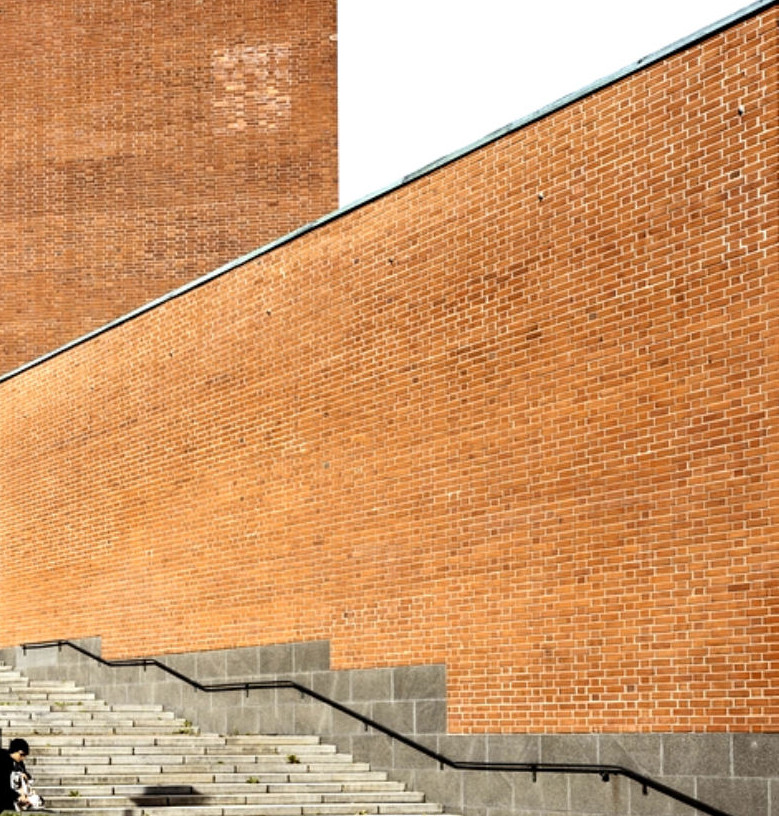
\includegraphics[width=\textwidth]{ch09/figures/briko.jpg}
    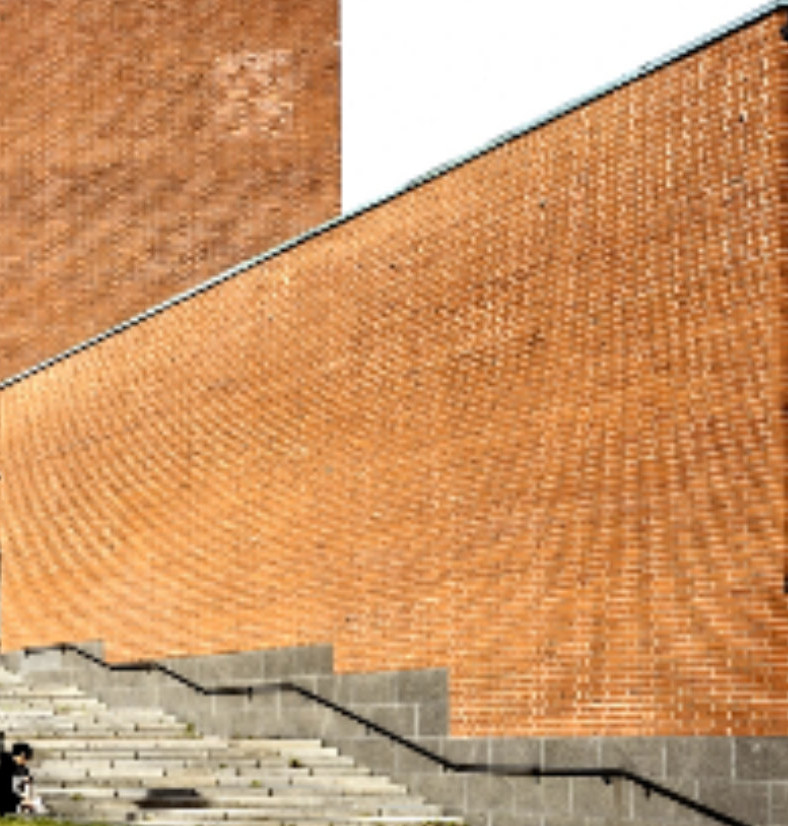
\includegraphics[width=\textwidth]{ch09/figures/brickd.jpg}
  \end{center}
  \caption{Example of aliasing behavior in a 2D image. Above: original, Below: aliased. When scaling an image (reducing its size),
    it is important to apply an anti-aliasing filter that removes high frequency spectral components from the
    high resolution image before it is scaled down to a lower resolution. Otherwise, there is a risk that 
    high frequency periodic structures
    will appear as low frequency structures in the scaled image, as shown in the lower image.
    Anti-aliasing filtering is a standard feature of most image processing libraries, and one rarely 
    sees the type of aliasing shown in the bottom figure in practice.}
  \label{fig:brick_alias}
\end{marginfigure}
To study aliasing behavior in 2D, it is sufficient to study aliasing effects on individual spectral components:
\begin{equation}
  z(x,y) = a e^{i (\omega_1 x + \omega_2 y) }\,\,,
\end{equation}
When discretizing the 2D complex exponential spectral component, one can obtain aliasing behavior 
when sampling through $2\pi$-periodicity:
\begin{align}
  z[n,m] & = a e^{i(\omega_1 T_x n + \omega_2 T_y m ) }                                \\
         & =a e^{i([\omega_1 T_x + 2\pi k]n + [\omega_2 T_y + 2\pi \ell]m)}            \\
         & =a e^{i([\hat{\omega}_1 + 2\pi k]n + [\hat{\omega}_{2} + 2\pi \ell]m)}\,\,.
\end{align}
Here $k,l \in \mathbb{Z}$.

Figure \ref{fig:brick_alias} demonstrates aliasing in 2D. This is
discretized in such a way that the high spatial frequency brick
pattern on the side of the building becomes undersampled, and a low
frequency alias is seen.


\subsection{Reconstruction}
\begin{marginfigure}
  \tikzstyle{int}=[draw, minimum size=2em]
  \tikzstyle{init} = [pin edge={to-,thin,black}]
  \begin{center}
    %  \resizebox{\columnwidth}{!}{%
    \begin{tikzpicture}[every text node part/.style={align=center},node distance=3cm,auto,>=latex']
      \node [int] (a) {D-to-C \\ $T_s$};
      \node (b) [left of=a,node distance=2cm, coordinate] {a};
      %    \node (c) [below=a,node distance=3cm] {a};

      %\node [int, pin={[init]above:$p_0$}] (c) [right of=a] {$\frac{1}{s}$};
      \node [coordinate] (end) [right of=a, node distance=3cm]{};
      \path[->] (b) edge node {$x[n]$} (a);
      \draw[->] (a) edge node {$x(t)$} (end) ;
    \end{tikzpicture}
    % }
  \end{center}
  \caption{A Discrete-time to Continuous-time (D-to-C) converter.}
\end{marginfigure}

Reconstruction involves transforming a discrete-time signal into a continuous-time signal. 
This type of operation is done, e.g., when
translating an audio signal into air pressure variations to create sound.

In order to convert a discrete-time signal into a continuous-time signal, some form 
of interpolation is needed in order to fill in the space between the samples. 
This is the function of a reconstruction filter, or a discrete-time to continuous-time (D-to-C) system:
\begin{equation}
  x(t) = \mathcal{R}\{x[n]\}\,\,.
\end{equation}
The ingredients that are needed to reconstruct the signal are the samples $x[n]$, information about the
sampling rate $T_s=1/f_s$, and information about the Nyquist zone that the signal is within.

This is equivalent to knowing the true values of the discrete-time frequencies $\hat{\omega}$ of all the discretized spectral
components, i.e., being able to rule out all the aliases using a priori knowledge of the frequency band that the signal lies in.

There are several ways to perform this reconstruction. If the analytical form of the signal is 
known, as in the case of a sinusoid, the signal can be generated analytically based on the 
phase and amplitude of the signal. In other cases, some form of interpolation is needed.

\subsection{Interpolation filters}
In this section, we'll only cover reconstruction of oversampled signals\footnote{It is possible to derive interpolation filters
  for reconstruction of undersampled signals in the same way, but this is beyond the scope of this course.} that satisfy
the Nyquist-Shannon sampling criterion $f_s > 2f_{\mathrm{max}}$, i.e., 
the spectral components of the signal are between $-f_s/2 < f < f_s/2$.

We can convert a discrete-time signal into a continuous-time signal using an interpolation filter of the form:
\begin{equation}
  x(t) = \sum_{n=-\infty}^{\infty} x[n]p(t-nT_s)\,\,.
\end{equation}
Theoretically, this interpolation filter can use the discrete-time samples to obtain the continuous-time reconstruction.
\begin{marginfigure}
  \begin{center}
    \begin{tikzpicture}
      \begin{axis}[domain=-5:5,
          width=7cm,height=7cm,ymin=-1.2,xmin=-4,ymax=2.4,xmax=4,
          ytick={-1,1},
          yticklabels={$-A$, $A$},
          xlabel=$t$, axis lines = center]
        \addplot[samples=400]{cos(deg(2.0*3.1415*0.2*x))};
        \addplot+[ycomb,samples=11]{cos(deg(2.0*3.1415*0.2*x))};
        \addplot[mark=none,color=gray] plot coordinates {(-4.5,0.30901699) (-3.5,0.30901699) (-3.5,-0.80901699) (-2.5,-0.80901699) (-2.5,-0.80901699) (-1.5,-0.80901699) (-1.5,0.30901699) (-0.5,0.30901699) (-0.5,1.) (0.5,1.) (0.5,0.30901699) (1.5,0.30901699) (1.5,-0.80901699) (2.5,-0.80901699) (2.5,-0.80901699) (3.5,-0.80901699)  (3.5,0.30901699) (4.5,0.30901699)};

        \addplot[mark=none,color=blue] plot coordinates {(-0.5,0.0) (-0.5,1.0) (0.5,1.0) (0.5,0)};                             %  \addplot[samples=100,domain=-0.5:0.5,color=blue]{1};

        \legend{Original signal,Samples, Reconstruction, $p(t)$}
      \end{axis}
    \end{tikzpicture}
  \end{center}
  \caption{Zero-order hold interpolation.}
  \label{fig:z-o-hold}
\end{marginfigure}

\newthought{The zero-order hold filter} is the simplest interpolation filter. 
It obtains a constant value for the duration of a sample.
The filter in this case has the following mathematical definition:
\begin{equation}
  p(t) = \left\{
  \begin{array}{rcr}
    1 & \mathrm{when}      & -\frac{T_s}{2} < t \le \frac{T_s}{2} \\
    0 & \mathrm{otherwise} &                                      \\
  \end{array}
  \right\} \,\,.
\end{equation}
The generated continuous-time signal looks like the one shown in Figure \ref{fig:z-o-hold}.

\begin{marginfigure}
  \begin{center}
    \begin{tikzpicture}
      \begin{axis}[domain=-5:5,
          width=7cm,height=7cm,ymin=-1.2,xmin=-4,ymax=2.4,xmax=4,
          ytick={-1,1},
          yticklabels={$-A$, $A$},
          xlabel=$t$, axis lines = center]
        \addplot[samples=400]{cos(deg(2.0*3.1415*0.2*x))};
        \addplot+[ycomb,samples=11]{cos(deg(2.0*3.1415*0.2*x))};
        \addplot[mark=none,color=gray] plot coordinates {(-4,0.30901699) (-3,-0.80901699) (-2,-0.80901699) (-1,0.30901699) (0.0,1.)  (1,0.30901699) (2,-0.80901699) (3,-0.80901699) (4,0.30901699) };
        \addplot[samples=100,domain=-1:1,color=blue]{1-abs(x)};

        \legend{Original signal,Samples, Reconstruction, $p(t)$}
      \end{axis}
    \end{tikzpicture}
  \end{center}
  \caption{Linear interpolation filter.}
  \label{fig:lin_int_filter}
\end{marginfigure}

The zero-order hold filter only needs one sample at a time. However, the continuous-time signal has large steps.
The zero-order hold filter approaches the continuous-time signal only when $T_s\rightarrow 0$ -- i.e., 
when the sample rate is infinitely large.

\newthought{A Linear interpolation filter} is defined as follows:
\begin{equation}
  p(t) = \left\{
  \begin{array}{rcr}
    1-\frac{|t|}{T_s} & \mathrm{when}      & -T_s < t < T_s \\
    0                 & \mathrm{otherwise} &                \\
  \end{array}
  \right\} \,\,.
\end{equation}
It applies a linear interpolation between two consecutive samples. The generated continuous-time signal 
is depicted in Figure \ref{fig:lin_int_filter}.

\newthought{The ideal reconstruction filter} is based on the
Shannon-Nyquist sampling theorem. It guarantees theoretically that a continuous-time real-valued signal 
can be perfectly reconstructed from discrete-time samples for
signals occupying the band $-f_s/2 < f < f_s/2$, if $f_s > 2f_{\mathrm{max}}$.
Here $f_{\mathrm{max}}$ is the maximum frequency component within the signal. We'll prove this 
theorem at the end of this chapter.

In order to reconstruct the signal perfectly in a mathematical sense, an ideal 
reconstruction filter must be used.
Something approximately resembling a truncated or tapered version of an ideal reconstruction filter is 
typically used in real world applications.

The form of this ideal reconstruction filter can be derived from the inverse Fourier transform of a 
rectangular shaped window that in frequency domain is an ideal low pass filter:
\begin{equation}
  P(\omega) = \left\{
  \begin{array}{rcr}
    T_s & \mathrm{when}      & |\omega| \le \pi f_s \\
    0   & \mathrm{otherwise} &                      \\
  \end{array}
  \right. \,\,.
\end{equation}
\begin{marginfigure}
  \begin{center}
    \begin{tikzpicture}
      \begin{axis}[domain=-5:5,
          width=7cm,height=7cm,ymin=-1.2,xmin=-4,ymax=2.4,xmax=4,
          ytick={-1,1},
          yticklabels={$-A$, $A$},
          xlabel=$t$, axis lines = center]
        \addplot[samples=400]{cos(deg(2.0*3.1415*0.2*x))};
        \addplot+[ycomb,samples=11]{cos(deg(2.0*3.1415*0.2*x))};
        \addplot[samples=400,mark=none,color=gray]{cos(deg(2.0*3.1415*0.2*x))};
        \addplot[samples=100,domain=-4:4,color=blue]{sin(deg((3.14)*(x+0.0000001)))/(3.14*(x+0.000001))};

        \legend{Original signal,Samples, Reconstruction,$p(t)$}
      \end{axis}
    \end{tikzpicture}
  \end{center}
  \caption{Ideal reconstruction filter.}
\end{marginfigure}
Here $P(\omega)$ is the Fourier transform of the reconstruction
filter, $\omega$ is angular frequency. The resulting ``ideal''
reconstruction filter is:
\begin{align}
  p(t) & =\frac{1}{2\pi}\int_{-\infty}^{\infty} P(\omega)e^{i\omega t}d\omega \\
       & = \frac{T_s}{\pi t}\sin\left(\frac{\pi}{T_s}t\right)\,\,.
\end{align}
This filter is infinitely long, which implies that all samples need to be used in order for the 
reconstructed signal to be mathematically perfect.

\if 0
  Similar reconstruction filters exists for other Nyquist zones, which allow perfect 
  reconstruction of undersampled signals, which satisfy the Shannon-Nyquist sampling criterion. 
  Such filters use ideal reconstruction filters that can be derived from idealized band-pass filters:
  \begin{equation}
    P(\omega) = \left\{
    \begin{array}{rcr}
      T_s & \mathrm{when}      & k\omega_s/2 \le |\omega| < (k+1)\omega_s/2 \\
      0   & \mathrm{otherwise} &                                            \\
    \end{array}
    \right\} \,\,.
  \end{equation}
  Here $k$ specifies the Nyquist zone for which the signal is to be reconstructed in.
\fi

\section{Shannon's sampling theorem}
\begin{marginfigure}
  \begin{center}
    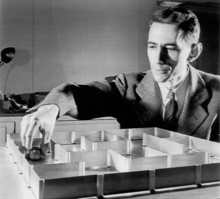
\includegraphics[width=\textwidth]{ch09/figures/shannon_mouse.png}
  \end{center}
  \caption{Claude Elwood Shannon. Photo: Bell Labs.}
\end{marginfigure}

Shannon's sampling theorem is a fundamental theorem in information theory and signal 
processing\sidenote{This theorem was discovered by Edmund Whittaker 33 years before Claude Shannon, 
and thus sometimes the sampling theory is called the Whittaker-Shannon sampling theorem.\cite{whittaker1915xviii,shannon1948mathematical}}. 
It relates the sample-rate of a discrete-time signal to the bandwidth of a continuous-time signal in frequency domain.
The full form of the theory is not just: ``use a sample-rate that is at least twice as large as the largest 
frequency component in the continuous-time signal''. There are other solutions, which also guarantee that no 
information about the signal is lost.
The most general way to investigate if information is lost when discretizing a signal is to explore 
the relationship between the Fourier transform of the signal, and the Fourier transform of the discretized signal.

We will assume that information is contained in the shape of the signal $x(t)$. 
This signal is assumed to be band-limited in frequency domain.
This means that the spectrum is zero valued outside a certain range of frequencies: 
$\hat{x}(\omega) = 0$ when $\omega < \omega_{\mathrm{min}}$ or $\omega > \omega_{\mathrm{max}}$.

Is it possible to form a discrete-time signal $x[n]$ from $x(t)$ in such a way that $x[n]$ contains sufficient information to
allow us to perfectly reconstruct $x(t)$? In other words, can we perfectly reconstruct a continuous-time signal $x(t)$ from
its discrete-time representation? This is the question that Shannon studied, and his sampling theorem provides an answer to.

\subsection{Sampling}
\begin{marginfigure}[3cm]
  \begin{center}
    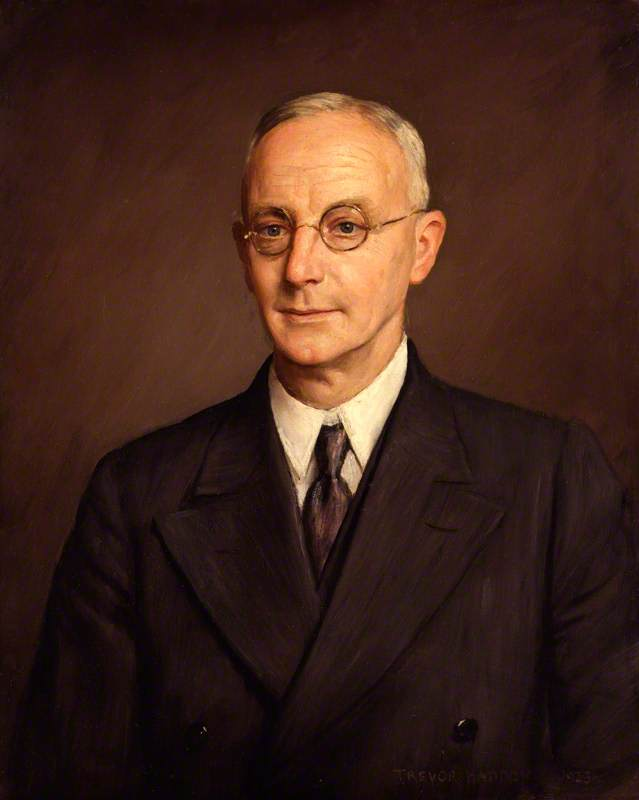
\includegraphics[width=\textwidth]{ch09/figures/whittaker.jpg}
  \end{center}
  \caption{Sir Eduard Whittaker. Photo: National Portrait Gallery.}
\end{marginfigure}

In the idealized case, sampling of a signal is selection of samples from a continuous-time signal:
\begin{equation}
  x[n] = x(nT_s)
\end{equation}
where $T_s$ is the sample spacing. This is the inverse of the sample-rate $T_s = f_s^{-1}$. 
We can express this sampling process using the Dirac delta function, 
where a delayed Dirac delta ``samples'' the value of the signal $x(t)$ at time $nT_s$:
\begin{equation}
  x[n] = \int_{-\infty}^{\infty}x(t)\delta(t-nT_s)dt = x(nT_s).
\end{equation}
We can use a train of Dirac delta functions (Dirac comb)
\begin{equation}
  s(t) = \sum_{n=-\infty}^{\infty}\delta(t-nT_s),
\end{equation}
to represent the sampled signal in continuous-time:
\begin{align}
  x_s(t) & = x(t) s(t)                                     \\
         & = x(t) \sum_{n=-\infty}^{\infty} \delta(t-nT_s) \\
         & = \sum_{n=-\infty}^{\infty} x[n]\delta(t-nT_s)
\end{align}
The sampled signal $x_s(t)$ is a continuous-time signal, which has the same information 
content as the array of samples $x[n]$. This means that $x_s(t)$ can be formed just by 
knowledge of the discrete-time signal $x[n]$.

\subsection{Fourier series representation for Dirac comb}
The Dirac comb
\begin{equation}
  s(t) = \sum_{k=-\infty}^{\infty} \delta(t-kT_s),
\end{equation}
is a periodic function with period $T_s$. Therefore, it is possible to express it as a Fourier series:
\begin{equation}
  s(t) = \sum_{k=-\infty}^{\infty} c_k e^{i\frac{2\pi}{T_s}kt}.
\end{equation}
The coefficients of the Fourier series can be obtained using the Fourier series synthesis equation, 
by integrating over one period of the function:
\begin{align}
  c_k & = \frac{1}{T_s}\int_{-T_s/2}^{T_s/2} \left[\sum_{n=-\infty}^{\infty} \delta(t-nT_s) \right] e^{-i\frac{2\pi}{T_s}kt}dt \\
      & =\frac{1}{T_s}\int_{-T_s/2}^{T_s/2} \delta(t)  e^{-i\frac{2\pi}{T_s}kt}dt                                              \\
      & =\frac{1}{T_s}e^{-i\cdot 0}                                                                                            \\
      & =\frac{1}{T_s}
\end{align}
We also note that $2\pi/T_s = \omega_s$, which is the sample-rate expressed as an angular frequency. 
The Fourier series representation of the Dirac-comb is therefore:
\begin{equation}
  s(t) = \frac{1}{T_s}\sum_{k=-\infty}^{\infty} e^{i k \omega_s t}.
\end{equation}
This Fourier series representation can now be substituted to represent the sampling operation as:
\begin{align}
  x_s(t) & = x(t)s(t)                                                                     \\
         & = x(t)  \left(\frac{1}{T_s}\sum_{k=-\infty}^{\infty} e^{i k \omega_s t}\right)
\end{align}

\subsection{Spectral representation of $x_s(t)$ and $x(t)$}
We then Fourier transform $x_s(t)$ to study the relationship between the sample-rate and 
the bandwidth of the signal.
We use the property that multiplication in time domain is convolution in frequency domain. 
The Fourier transform of $x(t)$ is $\hat{x}(\omega)$.
The Fourier transform of $s(t)$ is $\hat{s}(\omega)$. We also make use of the fact that the 
Fourier transform of $e^{i k \omega_s t}$ is $2\pi\delta(\omega-k\omega_s)$:
\begin{align}
  \hat{x}_s(\omega) & = \frac{1}{2\pi}  \hat{x}(\omega)*\hat{s}(\omega)\label{eq:xs_spec}                                                                                            \\
                    & = \frac{1}{2\pi}\int_{-\infty}^{\infty}\hat{x}(\omega') \hat{s}(\omega-\omega')d\omega'                                                                        \\
                    & = \frac{1}{2\pi} \int_{-\infty}^{\infty} \hat{x}(\omega')\left(\frac{1}{T_s}\sum_{k=-\infty}^{\infty} 2\pi \delta(\omega- k\omega_s - \omega')\right) d\omega' \\
                    & = \frac{1}{T_s} \sum_{k=-\infty}^{\infty}\int_{-\infty}^{\infty} \hat{x}(\omega')\delta(\omega - k\omega_s - \omega') d\omega'                                 \\
                    & = \frac{1}{T_s} \sum_{k=-\infty}^{\infty} \hat{x}(\omega-k\omega_s).
\end{align}
In other words, the Fourier transform of the sampled function $x_s(t)$ is infinitely 
many copies of $\hat{x}(\omega)$, each shifted by $k\omega_s$ and scaled in 
amplitude by $\frac{1}{T_s}$.

We illustrate this using the following two figures. The first one depicts the magnitude 
spectrum of the original continuous-time signal $x(t)$:
\begin{center}
  \begin{tikzpicture}
    \begin{axis}[width=15cm,height=5cm,ymin=0,ymax=3,
        xmin=-11,xmax=11,
        xlabel={$\omega$},
        ylabel={$|\hat{x}(\omega)|$},
        axis x line=center,
        axis y line=center,
        yticklabels={,,,},
        xtick={-6,-3,3,6},
        xticklabels={$-\omega_s$,$-\omega_s/2$,$\omega_s/2$,$\omega_s$}
      ]
      \addplot[mark=none,color=blue] plot coordinates {(-10,0.0) (-1,0) (-0.8,2*0.8) (-0.2,2*1) (0,0) (0.2,2*1) (0.8,2*0.8) (1,0)  (7,0)};

    \end{axis}
  \end{tikzpicture}
\end{center}
The sampled signal $x_s(t)$ has a periodic spectrum $\hat{x}_s(\omega)
  = \hat{x}_s(\omega+k\omega_s)$, which has a period $\omega_s$:
\begin{center}
  \begin{tikzpicture}
    \begin{axis}[width=15cm,height=5cm,ymin=0,ymax=3,
        xmin=-11,xmax=11,
        xlabel={$\omega$},
        ylabel={$|\hat{x}_s(\omega)|$},
        axis x line=center,
        axis y line=center,
        yticklabels={,,,},
        xtick={-6,-3,3,6},
        xticklabels={$-\omega_s$,$-\omega_s/2$,$\omega_s/2$,$\omega_s$}
      ]
      \addplot[mark=none,color=blue] plot coordinates {(-10,0.0) (-7,0) (-6.8,2*0.8) (-6.2,2*1) (-6,0) (-5.8,2*1) (-5.2,2*0.8) (-5,0) (-1,0) (-0.8,2*0.8) (-0.2,2*1) (0,0) (0.2,2*1) (0.8,2*0.8) (1,0)  (5,0) (5.2,2*0.8) (5.8,2*1) (6,0) (6.2,2*1) (6.8,2*0.8) (7,0)};
      \draw node at (axis cs:-9,0.5) {$\cdots$};
      \draw node at (axis cs:9,0.5) {$\cdots$};
    \end{axis}
  \end{tikzpicture}
\end{center}
This probably already provides some idea of what the sample-rate should be, in order to 
avoid losing information. The most straightforward answer is that if the spectrum of the 
original signal $\hat{x}(\omega)$ is confined within the limits of $\pm \omega_s/2$, 
then no overlap between the different copies of $\hat{x}(\omega)$ occurs.

There are other solutions that avoid aliasing for real-valued signals. The original 
signal $\hat{x}(\omega)$ might also be confined in frequency to one of 
the intervals $n \omega_s/2 \le |\omega| < (n+1)\omega_s/2$ with $n\in\mathbb{Z}$.
This property is widely used when sampling radio signals that are at a much higher 
frequency than the sample rate. This type of sampling strategy is called undersampling.

\subsection{Aliasing}
If the different copies of $\hat{x}(\omega)$ in $\hat{x}_s(\omega)$ overlap, then 
aliasing occurs. For example, if the spectrum of $\hat{x}(\omega)$ extends over the 
limits $\pm \omega_s/2$, then there are regions where $\hat{x}_s(\omega)$ is occupied 
by two or more spectral components of $\hat{x}(\omega)$ at the same time.

If the frequency extent of the original signal $\hat{x}(\omega)$ is larger than $\omega_s$, 
then aliasing occurs as shown below:
\begin{center}
  \begin{tikzpicture}
    \begin{axis}[width=15cm,height=5cm,ymin=0,ymax=3,
        xmin=-11,xmax=11,
        xlabel={$\omega$},
        ylabel={},
        axis x line=center,
        axis y line=center,
        yticklabels={,,,},
        xtick={-6,-3,3,6},
        xticklabels={$-\omega_s$,$-\omega_s/2$,$\omega_s/2$,$\omega_s$}
      ]
      \addplot[mark=none,color=blue] plot coordinates {(-10,0.0) (-9.5,0) (-6.8,2*0.8) (-6.2,2*1) (-6,0) (-5.8,2*1) (-5.2,2*0.8) (-2.5,0) (-3.5,0) (-0.8,2*0.8) (-0.2,2*1) (0,0) (0.2,2*1) (0.8,2*0.8) (3.5,0)  (2.5,0) (5.2,2*0.8) (5.8,2*1) (6,0) (6.2,2*1) (6.8,2*0.8) (9.5,0) (10,0) } ;
      \addlegendentry{$\hat{s}(\omega + k\omega_s)$}
      \addplot[mark=none,color=red] plot coordinates {(-9.5,0.5775) (-8.5,0.5775) (-6.8,2*0.8) (-6.2,2*1) (-6,0) (-5.8,2*1) (-5.2,2*0.8) (-3.5,0.5775) (-2.5,0.5775) (-0.8,2*0.8) (-0.2,2*1) (0,0) (0.2,2*1) (0.8,2*0.8) (2.5,0.5775)  (3.5,0.5775) (5.2,2*0.8) (5.8,2*1) (6,0) (6.2,2*1) (6.8,2*0.8) (8.5,0.5775) (9.5,0.5775)};
      \addlegendentry{$\hat{x}_s(\omega)$}
      \draw node at (axis cs:-10,0.5) {$\cdots$};
      \draw node at (axis cs:10,0.5) {$\cdots$};

      %    \addplot[mark=none,color=blue] plot coordinates {(-10,0.0) (-7,0) (-6.8,2*0.8) (-6.2,2*1) (-6,0) (-5.8,2*1) (-5.2,2*0.8) (-5,0) (-1,0) (-0.8,2*0.8) (-0.2,2*1) (0,0) (0.2,2*1) (0.8,2*0.8) (1,0)  (5,0) (5.2,2*0.8) (5.8,2*1) (6,0) (6.2,2*1) (6.8,2*0.8) (7,0) } ;
    \end{axis}
  \end{tikzpicture}
\end{center}
In this case, positive and negative frequency components of the original spectrum $\hat{x}_s(\omega)$ 
overlap and are added together when $|\omega| > \omega_s/2$,
making it impossible to determine what the original value of $\hat{x}(\omega)$ is within the overlapping region.

\subsection{Complex-valued signal}
For a complex-valued signal $x(t)\in \mathbb{C}$, a sufficient condition for avoiding $\hat{x}(\omega)$ 
overlapping with itself in $\hat{x}_s(\omega)$ (aliasing) is that $\omega_s > \omega_{\mathrm{max}}-\omega_{\mathrm{min}}$.

Aliasing with complex signals is illustrated with the following plots. Consider a signal, which spans 
between frequencies $0.11\omega_s$ and $1.1\omega_s$.
In this case, the signal crosses $\omega_s/2$, which violates aliasing rules for real-valued signals. 
However, $\omega_s > \omega_{\mathrm{max}}-\omega_{\mathrm{min}}$.
\begin{center}
  \begin{tikzpicture}
    \begin{axis}[width=15cm,height=5cm,ymin=0,ymax=3,
        xmin=-11,xmax=11,
        xlabel={$\omega$},
        ylabel={$\hat{x}(\omega)\in \mathbb{C}$},
        axis x line=center,
        axis y line=center,
        yticklabels={,,,},
        xtick={-6,-3,3,6},
        xticklabels={$-\omega_s$,$-\omega_s/2$,$\omega_s/2$,$\omega_s$}
      ]
      \addplot[mark=none,color=blue] plot coordinates {(-10,0) (1.2,0) (2,0.5) (6,1) (7,0) (10,0) } ;

    \end{axis}
  \end{tikzpicture}
\end{center}
The spectrum of the sampled signal $x_s(t)$ has a periodic spectrum
$\hat{x}_s(\omega) = \hat{x}_s(\omega+k\omega_s)$. Notice that there
is no overlap between the copies of the spectrum:
\begin{center}
  \begin{tikzpicture}
    \begin{axis}[width=15cm,height=5cm,ymin=0,ymax=3,
        xmin=-11,xmax=11,
        xlabel={$\omega$},
        ylabel={$|\hat{x}_s(\omega)|$},
        axis x line=center,
        axis y line=center,
        yticklabels={,,,},
        xtick={-6,-3,3,6},
        xticklabels={$-\omega_s$,$-\omega_s/2$,$\omega_s/2$,$\omega_s$}
      ]
      \addplot[mark=none,color=blue] plot coordinates {(-10,0) (1.2,0) (2,0.5) (6,1) (7,0) (10,0) } ;
      \addplot[mark=none,color=blue] plot coordinates {(-10,0) (1.2+6,0) (2+6,0.5) (6+6,1) (7+6,0) (10+6,0) } ;

      \addplot[mark=none,color=blue] plot coordinates {(-10,0) (1.2-6,0) (2-6,0.5) (6-6,1) (7-6,0) (10-6,0) } ;
      \addplot[mark=none,color=blue] plot coordinates {(-10-12,0) (1.2-12,0) (2-12,0.5) (6-12,1) (7-12,0) (10-12,0) } ;

      \draw node at (axis cs:-9,0.5) {$\cdots$};
      \draw node at (axis cs:9,0.5) {$\cdots$};

      %    \addplot[mark=none,color=blue] plot coordinates {(-10,0.0) (-7,0) (-6.8,2*0.8) (-6.2,2*1) (-6,0) (-5.8,2*1) (-5.2,2*0.8) (-5,0) (-1,0) (-0.8,2*0.8) (-0.2,2*1) (0,0) (0.2,2*1) (0.8,2*0.8) (1,0)  (5,0) (5.2,2*0.8) (5.8,2*1) (6,0) (6.2,2*1) (6.8,2*0.8) (7,0) } ;
    \end{axis}
  \end{tikzpicture}
\end{center}
This means that the values of $\hat{x}_s(\omega)$ between, e.g., $0.11\omega_s$ and $1.1\omega_s$ fully 
determine the frequency domain representation of the original signal $\hat{x}(\omega)$.

\subsection{Sampling criteria}
The Shannon-Nyquist sampling theorem requires that it should be possible to reconstruct $\hat{x}(\omega)$ from
$\hat{x}_s(\omega)$. The commonly described criterion that requires the sample-rate to be higher than twice the 
largest frequency component of the signal:
\begin{equation}
  f_s > 2 f_\mathrm{max}
\end{equation}
is just one possible solution, which assumes that the spectral components within the 
original signal $\hat{x}(\omega)$ are confined to $|f| < f_s/2$. As we discussed above, 
complex-valued signals and under sampled signals result in different sampling criteria.

\subsection{Reconstruction}
This reconstruction strategy only applies to a real-valued signal $x(t) \in \mathbb{R}$ 
within the principal spectrum.
It should be easy to determine how to create a reconstruction filter for, e.g., a 
complex-valued signal occupying the band $\omega \in [\omega_{\mathrm{min}},\omega_{\mathrm{max}}]$ 
after following this derivation.

In order to reconstruct signal $x(t)$ from $x[n]$, we first form $x_s(t)$ using $x[n]$:
\begin{equation}
  x_s(t) = \sum_{n=-\infty}^{\infty} x[n]\delta(t-n T_s)
\end{equation}
We then use an ideal low-pass filter specified in frequency domain as:
\begin{equation}
  \Hiw = \left\{ \begin{array}{cc}
    T_s & |\omega| \le \frac{\omega_s}{2} \\
    0   & \mathrm{otherwise}
  \end{array}
  \right.
\end{equation}
When we apply this filter $\hat{x}_s(\omega)$ to reconstruct $\hat{x}(\omega)$:
\begin{align}
  \Hiw \hat{x}_s(\omega) & = \Hiw\frac{1}{T_s} \sum_{k=-\infty}^{\infty} \hat{x} (\omega-k\omega_s) \\
                         & = \hat{x}(\omega) \qed
\end{align}
This operation is shown in the Figure below:
\begin{center}
  \begin{tikzpicture}
    \begin{axis}[width=15cm,height=5cm,ymin=0,ymax=3,
        xmin=-11,xmax=11,
        xlabel={$\omega$},
        ylabel={$|\hat{x}_s(\omega)|$},
        axis x line=center,
        axis y line=center,
        yticklabels={,,,},
        xtick={-6,-3,3,6},
        xticklabels={$-\omega_s$,$-\omega_s/2$,$\omega_s/2$,$\omega_s$}
      ]
      \addplot[mark=none,color=blue] plot coordinates {(-10,0.0) (-9.0,0) (-6.8,2*0.8) (-6.2,2*1) (-6,0) (-5.8,2*1) (-5.2,2*0.8) (-3,0) (-3,0) (-0.8,2*0.8) (-0.2,2*1) (0,0) (0.2,2*1) (0.8,2*0.8) (3,0)  (3,0) (5.2,2*0.8) (5.8,2*1) (6,0) (6.2,2*1) (6.8,2*0.8) (9,0) (10,0) } ;
      \draw node at (axis cs:-10,0.5) {$\cdots$};
      \draw node at (axis cs:10,0.5) {$\cdots$};
      \draw node at (axis cs:3.5,2.5) {$\Hiw$};
      \addplot[mark=none,color=red] plot coordinates {(-10,0.0) (-3,0) (-3,2.2) (3,2.2) (3,0) (10,0) } ;

      %    \addplot[mark=none,color=blue] plot coordinates {(-10,0.0) (-7,0) (-6.8,2*0.8) (-6.2,2*1) (-6,0) (-5.8,2*1) (-5.2,2*0.8) (-5,0) (-1,0) (-0.8,2*0.8) (-0.2,2*1) (0,0) (0.2,2*1) (0.8,2*0.8) (1,0)  (5,0) (5.2,2*0.8) (5.8,2*1) (6,0) (6.2,2*1) (6.8,2*0.8) (7,0) } ;
    \end{axis}
  \end{tikzpicture}
  \begin{tikzpicture}
    \begin{axis}[width=15cm,height=5cm,ymin=0,ymax=3,
        xmin=-11,xmax=11,
        xlabel={$\omega$},
        ylabel={$|\hat{x}(\omega)|$},
        axis x line=center,
        axis y line=center,
        yticklabels={,,,},
        xtick={-6,-3,3,6},
        xticklabels={$-\omega_s$,$-\omega_s/2$,$\omega_s/2$,$\omega_s$}
      ]
      \addplot[mark=none,color=blue] plot coordinates {(-10,0.0)  (-3,0) (-0.8,2*0.8) (-0.2,2*1) (0,0) (0.2,2*1) (0.8,2*0.8) (3,0)   (10,0) } ;

      ;
    \end{axis}
  \end{tikzpicture}
\end{center}
This is in essence the proof of Shannon's sampling theorem. To obtain $x(t)$, 
one can use an inverse Fourier transform:
\begin{equation}
  x(t) = \frac{1}{2\pi}\int_{-\infty}^{\infty} \hat{x}(\omega) e^{i\omega t}d\omega.
\end{equation}
If $\hat{x}_s(\omega)$ contains overlapping copies of $\hat{x}(\omega)$, then the original 
spectrum $\hat{x}(\omega)$, and therefore the original signal $x(t)$, cannot be reconstructed.

For a comple- valued signal, we would need to apply an ideal band-pass filter, which only 
retains signals between $\omega_{\mathrm{min}}$ and
$\omega_{\mathrm{max}}$, instead of the ideal low-pass filter. The same applies to an undersampled signal.

\subsection{Ideal reconstruction filter}
Recall, from the beginning of this course, that we introduced the ideal reconstruction filter without deriving it. 
Now we can derive it. It is the inverse Fourier transform of the ideal low-pass filter
\begin{equation}
  \Hiw = \left\{ \begin{array}{cc}
    T_s & |\omega| \le \frac{\omega_s}{2} \\
    0   & \mathrm{otherwise}
  \end{array}
  \right.
\end{equation}
which is
\begin{align}
  h(t) & = \frac{1}{2\pi}\int_{-\infty}^{\infty} \Hiw e^{i\omega t}d\omega                             \\
       & = \frac{1}{2\pi} \int_{-\omega_s/2}^{\omega_s/2} T_s e^{i\omega t}d\omega                     \\
       & = \frac{T_s}{2 \pi}\left. \frac{e^{i\omega t}}{it} \right|_{\omega=-\omega_s/2}^{\omega_s/2}  \\
       & = \frac{T_s}{2 t \pi i}\left( e^{i\frac{\omega_s}{2} t}  - e^{-i\frac{\omega_s}{2} t} \right) \\
       & = \frac{T_s}{\pi t} \sin(\frac{\omega_s}{2}t)                                                 
\end{align}
Keeping in mind that $\omega_s/2 = \pi/T_s$ we obtain the familiar result:
\begin{equation}
  \boxed{
    h(t) = \frac{T_s}{\pi t}\sin(\frac{\pi}{T_s}t)
  }
\end{equation}
When applying this reconstruction filter in time domain, one convolves the sampled signal to obtain the 
reconstructed continuous-time signal:
\begin{align}
  x(t) & = h(t)*x_s(t)                                                                                            \\
       & = \int_{-\infty}^{\infty} x_s(\tau)h(t-\tau)d\tau                                                        \\
       & = \int_{-\infty}^{\infty}\left( \sum_{n=-\infty}^{\infty} x[n] \delta(\tau-n T_s)\right) h(t-\tau) d\tau \\
       & = \sum_{n=-\infty}^{\infty} x[n] \int_{-\infty}^{\infty} \delta(\tau-nT_s) h(t-\tau)d\tau                \\
       & = \sum_{n=-\infty}^{\infty} x[n] \frac{\sin(\frac{\pi}{T_s}(t-n T_s))}{\frac{\pi}{T_s}(t-nT_s)}.
\end{align}
This reconstruction formula now perfectly reproduces $x(t)$ from
samples $x[n]$, provided that $\omega_s \ge 2\omega_{\mathrm{max}}$.

For an undersampled real-valued signal, or a complex-valued band limited signal, the ideal reconstruction 
filter would be different. In this case, it would correspond to the impulse response of an ideal band-pass filter.

\newpage
\section{Exercises: Discrete-time Signals}

\begin{enumerate}
  % Exercise 1
  \item The signal $x(t) = A e^{i\omega_0 t}$ is discretized using an idealized continuous-to-discrete 
        time converter $x[n]=x(n T_s)=Ae^{i\hat{\omega}_{k}n}$. Here $A=1$ and $\omega_0=2\pi 10042$ 
        radians per second. The sample rate is $f_s=100$ samples per second and $T_s=1/f_s$.
        \begin{enumerate}[a)]
          % Exercise 1a)
          \item What are all the possible values of $\hat{\omega}_k$ that result in an identical 
                discrete-time signal $x[n]$. Use normalized angular frequency with units of 
                radians per sample. The possible values $\hat{\omega}_k$ are called 
                frequency aliases. Here $k\in \mathbb{Z}$ is an integer index to the 
                different solutions.
          % Exercise 1b)
          \item What are the principal aliases in normalized angular frequency with units 
                radians per sample? Principal aliases are values of $\hat{\omega}_k$ that 
                lie in the interval $-\pi < \hat{\omega}_k < \pi$.
          % Exercise 1c)
          \item Draw the spectrum of this signal with normalized angular frequency in units of 
                radians per sample on the horizontal axis. Use the range $-3\pi < \hat{\omega} < 3\pi$. 
                How many frequency components are there?
          % Exercise 1d)
          \item There are infinitely many continuous-time signals $x_k(t)=A e^{i\omega_k t}$ 
                that will result in the same $x[n]$. What are all the possible continuous-time 
                angular frequencies $\omega_k$? What is the smallest possible absolute value of $|\omega_k|$?
          % Exercise 1e)
          \item What is the smallest possible sample-rate $f_s$ at which the signal $x(t)$ can be sampled at, 
                while still retaining enough information to allow the signal to be reconstructed?
        \end{enumerate}

  % Exercise 2
  \item Given the discrete-time sinusoid $y_1[n] = 2 \cos(0.67 \pi n) + \cos(0.33 \pi n)$.
        \begin{enumerate}[a)]
          % Exercise 2a)
          \item Draw the spectrum for $y_1[n]$. Show aliases in the normalized angular 
                frequency range $-3\pi < \hat{\omega} < 3\pi$ (radians per sample). 
                Label the principal spectrum showing the phase, amplitude and normalized 
                angular frequency of each frequency component.
          % Exercise 2b)
          \item Show how the spectrum changes if the signal changes to 
                $y_2[n] = 2 \cos(2.67 \pi n) + \cos(0.33 \pi n)$. 
                Use the same frequency range as in a).
        \end{enumerate}

  % Exercise 3
  \item If you've ever seen an old western movie with a stagecoach wheel seemingly 
        rotating in the wrong direction, this exercise will help you understand how 
        this optical illusion occurs. You have done a video recording of a disc with a 
        red mark on the rim. The disc started a clockwise rotation with slowly 
        increasing rotational speed $0 \le v_{rot} \le 2880$ rotations per minute (rpm). 
        The sampling rate of your camera was $f_s = 24$ frames per second (fps). 
        Assume that each frame is captured instantaneously, i.e., the exposure time is 
        infinitely short. On the recording, you can see that the red spot seems to 
        rotate differently for certain speeds and speed ranges.
        \begin{enumerate}[a)]
          % Exercise 3a)
          \item At what rotational speed (in rpm) does the red spot appear to be standing still?
          % Exercise 3b)
          \item Around a certain speed, the red spot appears to start to rotate 
                counter-clockwise, and for what speed range will this phenomenon occur?
          % Exercise 3c)
          \item Do you know another word for the counter-clockwise behavior?
          % Exercise 3d)
          \item What behavior does the red spot have beyond the speed found in a)?
        \end{enumerate}

  % Exercise 4
  \item The absolute values of the frequency domain representation of a signal is 
        shown in the figure below. We know that $\omega_{0}<\omega_{1}$ and:
        \begin{equation}
          |\hat{x}(\omega)| = \left\{\begin{array}{ccc}
            0  & \mathrm{when}      & \omega \ge \omega_1 \\
            0  & \mathrm{when}      & \omega \le \omega_0 \\
            >0 & \mathrm{otherwise} &
          \end{array}\right.,
        \end{equation}
        \begin{center}
          \begin{tikzpicture}
            \begin{axis}[width=15cm, height=4cm, ymin=0, ymax=2,
                xmin=-11,xmax=11,
                xlabel={$\omega$},
                ylabel={$|\hat{x}(\omega)|$},
                axis x line=center,
                axis y line=center,
                yticklabels={,,,},
                xtick={1.2,7},
                xticklabels={$\omega_0$,$\omega_1$}
              ]
              \addplot[mark=none,color=blue] plot coordinates {(-10,0) (1.2,0) (2,0.5) (6,1) (7,0) (10,0)};

            \end{axis}
          \end{tikzpicture}
        \end{center}
        \begin{enumerate}[a)]
          % Exercise 4a)
          \item $x(t)=(2\pi)^{-1}\int_{-\infty}^{\infty}\hat{x}(\omega)e^{i\omega t}d\omega$. 
                Why is $x(t)$ not a real-valued signal?
          % Exercise 4b)
          \item What is the minimum sample-rate (in units of samples per second) required 
                to retain all information about the signal?
          % Exercise 4c)
          \item Sketch a plot of $|\hat{x}_s(\omega)|$ for the sample rate you found 
                in b). $\hat{x}_s(\omega)$ is defined in Equation \ref{eq:xs_spec}. 
                Why don't the frequency shifted copies of $|\hat{x}(\omega)|$ overlap?
          % Exercise 4d)
          \item What reconstruction filter would be needed in order to perfectly 
                reconstruct $x(t)$ from the discretized signal $x[n]$, 
                using the sample-rate that you found?
        \end{enumerate}

  % Exercise 5
  \item The absolute values of the frequency domain representation of a signal is shown 
        in the figure below. We know that $\hat{x}(\omega)=\hat{x}^*(-\omega)$ and that:
        \begin{equation}
          |\hat{x}(\omega)| = \left\{\begin{array}{ccc}
            >0 & \mathrm{when}      & \omega_0 <|\omega| < \omega_1 \\
            0  & \mathrm{otherwise} &
          \end{array}\right.,
        \end{equation}
        We also know that $\omega_0 = 2\pi 30$ and $\omega_1 = 2\pi40$ (radians per second). 
        This signal is undersampled using a sample-rate of $f_s=20$ hertz (samples per second).
        \begin{center}
          \begin{tikzpicture}
            \begin{axis}[width=15cm,height=4cm,ymin=0,ymax=2,
                xmin=-50,xmax=50,
                xlabel={$\omega$},
                ylabel={$|\hat{x}(\omega)|$},
                axis x line=center,
                axis y line=center,
                yticklabels={,,,},
                xtick={-40,-30,30,40},
                xticklabels={$-\omega_1$,$-\omega_0$,$\omega_0$,$\omega_1$}
              ]
              \addplot[mark=none,color=blue] plot coordinates {(-50,0) (-40,0) (-32,1) (-30,0) (30,0) (32,1) (40,0) (50,0)};

            \end{axis}
          \end{tikzpicture}
        \end{center}
        \begin{enumerate}[a)]
          % Exercise 5a)
          \item $x(t)=(2\pi)^{-1}\int_{-\infty}^{\infty}\hat{x}(\omega)e^{i\omega t}d\omega$. 
                Is the signal $x(t)$ a real-valued signal?
          % Exercise 5b)
          \item Sketch a plot of $|\hat{x}_s(\omega)|$. Recall that $\hat{x}_s(\omega)$ is 
                defined in Equation \ref{eq:xs_spec}. Why don't the frequency shifted 
                copies of $|\hat{x}(\omega)|$ overlap?
          % Exercise 5c)
          \item The sample rate $f_s=20$ hertz is sufficient for retaining all information 
                about $x(t)$. Why?
          % Exercise 5d)
          \item What is the frequency domain definition of the perfect reconstruction filter that 
                reproduces the original continuous-time signal $x(t)$ from a sampled signal $x[n]$?
        \end{enumerate}

\end{enumerate}

 \ifSpExerciseSol
 \newpage
\section{Suggested solutions: Discrete-time Signals}
\begin{enumerate}
\item The signal $x(t)=Ae^{i\omega_{0}t}$ is discretized using an ideal continuous-to-discrete time converter $x[n]=x(nT_{s})=Ae^{i\hat{\omega}_{k}n}$. Let $A=1$ and $\omega_{0}=2\pi 10042$ rad/s. Let the sample rate be $f_{s}=100$ samples per second and $T_{s}=1/f_{s}$.

\begin{enumerate}[a)]
\item Have $\hat{\omega}_{0}=\omega_{0}T_{s}$ and $\hat{\omega}_{k}$ is
$$\hat{\omega}_{k}=\hat{\omega}_{0}+2\pi k=\omega_{0}\frac{1}{f_{s}}+2\pi k=\frac{5021}{25}\pi+2\pi k$$
for $k\in\mathbb{Z}$. 

\item The principal aliases lie in $-\pi<\hat{\omega}_{k}<\pi$. Pick a $k\in\mathbb{Z}$ such that $-\pi<\hat{\omega}_{k}<\pi$. For instance, $k=100$ works:
$$-\pi < \frac{5021}{25}\pi-2\pi 100 < \pi,$$
giving a value of $\hat{\omega}\approx2.6389\ \text{rad/sample}$. 

\item To draw the spectrum for $x(t)$ we can use the code in Listing \ref{plotcode1}.

\begin{lstlisting}[language=Python, caption=Spectrum of $x(t)$,label=plotcode1]
import numpy as n
import matplotlib.pyplot as plt

fs = 100 # sample-rate in Hz
om0 = 2*n.pi*fs

om = n.linspace(-3*n.pi,3*n.pi,num=1000)
plt.vlines(om0+2*n.pi*(-99),ymin=0,ymax=1,color="red")
plt.vlines(om0+2*n.pi*(-100),ymin=0,ymax=1,color="red")
plt.vlines(om0+2*n.pi*(-101),ymin=0,ymax=1,color="red")
plt.xlabel("$\hat{\omega}$")
plt.ylabel("$\hat{x}(\omega)$")
plt.grid(True)
plt.show()
\end{lstlisting}
The spectrum $\hat{x}(\omega)$ is shown in Figure \ref{spectrum_plot}. 
\begin{marginfigure}[1cm]
    \centering
    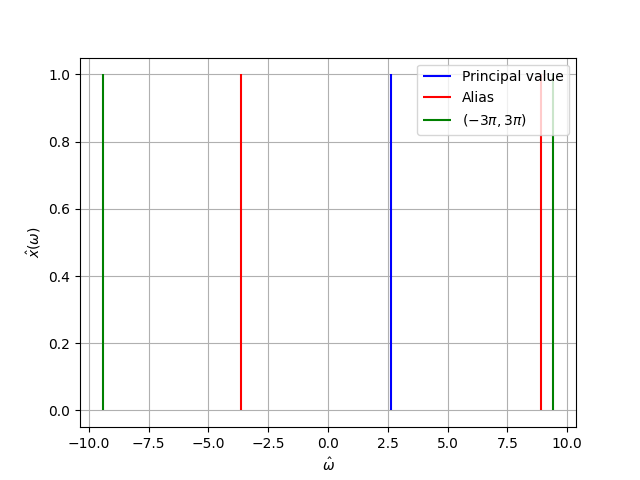
\includegraphics[width=\textwidth]{ch09/figures/spectrum_plot.png}
    \caption{Spectrum of $x(t)$, we see 3 spectral components in the range $(-3\pi,3\pi)$}
    \label{spectrum_plot}
\end{marginfigure}

\item The possible angular frequencies that result in the same discritization is found by
$$\omega_{k}=\omega_{0}+2\pi kf_{s}.$$
Choosing different values for $k$ and search for a value that satisfy the requirement of being the smallest $|\omega_{k}|$ is found to be $k=-100$. This value gives $\omega_{k}=2\pi42$. 

\item Here the signal is complex, so the signal can be sampled at $f_{s}>f_{\text{max}}-f_{\text{min}}=\frac{\omega_{0}}{2\pi}$ by the Shannon which correspond to $f_{s}>10042$ Hz. 
\end{enumerate}

\item Given the continuous-time sinusoid $y_1[n] = 2 \cos(0.67 \pi n) + \cos(0.33 \pi n)$.
  \begin{enumerate}[a)]
    \item Using Euler's formula to first rewrite $y_{1}[n]$ on polar form:\\
    	\[y_1[n] = e^{i0.67\pi n} + e^{-i0.67\pi n} + \frac{1}{2}e^{i0.33\pi n} + \frac{1}{2}e^{-i0.33\pi n}\]
    	and then plot the spectrum (Figure \ref{fig:ex1}):\\
		\begin{marginfigure}
		  \begin{center}
			\begin{tikzpicture}
			  \begin{axis}[
			    width=7cm,height=6cm,ymin=0,ymax=1.3,xmin=-3.1,xmax=3.2,  
			    ytick={0.5,1}, yticklabels={,$1$}, 
			    xtick={-3,...,3},
			    xticklabels={$-3\pi$,$-2\pi$,$-\pi$,$0$,$\pi$,$2\pi$,$3\pi$}, 
			    ylabel={$y[n]$}, 
			    xlabel={$\hat{\omega}$}, axis lines = center]
			    
				\addplot+[ycomb,mark=*,mark color=skyblue1, solid,
						color=skyblue1] plot coordinates {(-2.6,1)(2.6,1)};
			  	\node at (axis cs:-2.67,1)[above,
			  				font={\footnotesize}]{$e^{-i2.67\pi}$};
			  	\node at (axis cs:2.67,1)[below,
			  				font={\footnotesize}]{$e^{i2.67\pi}$};
			  	
				\addplot+[ycomb,mark=*,mark color=scarletred1, solid,
						color=scarletred1] plot coordinates {(-2.33,0.5)(2.33,0.5)};
			  	\node at (axis cs:-2.33,0.5)[above,
			  				font={\footnotesize}]{$\frac{1}{2}e^{-i2.33\pi}$};
			  	\node at (axis cs:2.33,0.5)[below,
			  				font={\footnotesize}]{$\frac{1}{2}e^{i2.33\pi}$};
			  	
				\addplot+[ycomb,mark=*,mark color=scarletred1, solid,
						color=scarletred1] plot coordinates {(-1.67,0.5)(1.67,0.5)};
			  	\node at (axis cs:-1.67,0.5)[below,
			  				font={\footnotesize}]{$\frac{1}{2}e^{-i1.67\pi}$};
			  	\node at (axis cs:1.67,0.5)[above,
			  				font={\footnotesize}]{$\frac{1}{2}e^{i1.67\pi}$};
			  	
				\addplot+[ycomb,mark=*,mark color=skyblue1, solid,
						color=skyblue1] plot coordinates {(-1.33,1)(1.33,1)};
			  	\node at (axis cs:-1.33,1)[below,
			  				font={\footnotesize}]{$e^{-i0.33\pi}$};
			  	\node at (axis cs:1.33,1)[above,
			  				font={\footnotesize}]{$e^{i0.33\pi}$};
			  	
			  	\addplot+[ycomb,mark=*,mark color=blue, solid,
						color=blue] plot coordinates {(-0.67,1)(0.67,1)};
			  	\node at (axis cs:-0.67,1)[above,
			  				font={\footnotesize}]{$e^{-i0.67\pi}$};
			  	\node at (axis cs:0.67,1)[below,
			  				font={\footnotesize}]{$e^{i0.67\pi}$};
			  	
				\addplot+[ycomb,mark=*,mark color=red, solid,
						color=red] plot coordinates {(-0.33,0.5)(0.33,0.5)};
			  	\node at (axis cs:-0.33,0.5)[above,
			  				font={\footnotesize}]{$\frac{1}{2}e^{-i0.33\pi}$};
			  	\node at (axis cs:0.33,0.5)[below,
			  				font={\footnotesize}]{$\frac{1}{2}e^{i0.33\pi}$};
			  	
			  \end{axis}
			\end{tikzpicture}
		  \end{center}
		\caption{Spectrum for 1.a): \\ $y_1[n] = 2 \cos(0.67 \pi n) + \cos(0.33 \pi n)$ \\ Shown only frequency components from principal up to 2nd alias.}
		\label{fig:ex1}
		\end{marginfigure}
    
    \item For the changed signal $y_2[n] = 2 \cos(2.67 \pi n) + \cos(0.33 \pi n)$, the spectrum will stay unchanged because $\cos(2.67 \pi n) = \cos(0.67 \pi n)$.
  \end{enumerate}
  
\item A sampling rate of 24 fps equals 1440 frames per minute.
\begin{enumerate}[a)]
    \item When the disc speed equals the camera's sampling rate at 1440 rpm, the red spot will be recorded at the same position for every frame, and thus appears to be standing still.
    \item When the disc speed gets larger than the Shannon-Nyquist sampling theorem, $v_{rot} > f_s / 2 > 720$ rpm, aliasing starts to occur. Within the speed range of $720 < v_{rot} < 1440$ rpm, the phase of the alias has the opposite sign than the phase of the real rotation, and so the red spot seems to rotate counter-clockwise with decreasing speed as $v_{rot}$ increases.
    \item Aliasing in the interval with opposite phase sign is called \emph{folding}.
    \item When $1440 < v_{rot} < 2880$, there is no folding, and the corresponding alias of the red spot will have speed $0 < v_{rot} < 1440$ rpm.
\end{enumerate}

\item Let $x(t)=(2\pi)^{-1}\int_{-\infty}^{\infty}\hat{x}(\omega)e^{i\omega t}d\omega$.

\begin{enumerate}[a)]
\item By the definition of $|\hat{x}(\omega)|$ and the Figure we see that there is no pairing for the frequencies, meaning that $\hat{x}^{*}(\omega)\neq \hat{x}(-\omega)$, so $x(t)$ can't be real.

\item For complex signals, we must sample at a rate that satisfy $f_{s}>f_{\text{max}}-f_{\text{min}}=\frac{1}{2\pi}(\omega_{1}-\omega_{0})$ in units of Hz. 

\item By the Shannon–sampling theorem the sample-rate $f_{s}$ from above is sufficient to retain all the information regarding the signal, thus the spectrum has no overlap. This is reflected in the drawing of $|\hat{x}_{s}(\omega)|$ where the copies are shown in red.

\begin{center}
\begin{tikzpicture}
\begin{axis}[width=15cm,height=4cm,ymin=0,ymax=2,
    	xmin=-11,xmax=11,
        xlabel={$\omega$},
        ylabel={$|\hat{x}_{s}(\omega)|$},
        axis x line=center, 
        axis y line=center, 
        yticklabels={,,,},
        xtick={1.2,7},
        xticklabels={$\omega_0$,$\omega_1$}
    ]
    \addplot[mark=none,color=red] plot coordinates {(-4.2,0) (7.0,0) (7.8,0.5) (11.8,1) (12.8,0) (15.8,0)};
    \addplot[mark=none,color=blue] plot coordinates {(-10,0) (1.2,0) (2,0.5) (6,1) (7,0) (10,0)};
    \addplot[mark=none,color=red] plot coordinates {(-15.8,0) (-4.6,0) (-3.8,0.5) (0.2,1) (1.2,0) (4.2,0)};
    \addplot[mark=none,color=red] plot coordinates {(-21.6,0) (-10.4,0) (-9.6,0.5) (-5.6,1) (-4.6,0) (-1.6,0)};
    \addplot[mark=none,color=red] plot coordinates {(-27.4,0) (-16.2,0) (-15.4,0.5) (-11.4,1) (-10.4,0) (-7.4,0)};
\end{axis}
\end{tikzpicture}
\end{center}

\item In this case, the reconstruction filter would be an ideal band-pass filter of the form
$$\mathcal{H}(\omega)=\begin{cases}
    T_{s}, \quad \omega_{1}\le\omega\le\omega_{2}, \\
    0, \quad \hspace{0.1cm}\text{otherwise}.
\end{cases}$$
Have $x_{s}(t)$ as
$$x_{s}(t)=\sum_{n=-\infty}^{\infty}x[n]\delta(t-nT_{s}),$$
from the samples. To reconstruct the signal, simply multiply $\hat{x}(\omega)$ by the reconstruction filter in frequency domain. The frequency domain representation of $x_{s}(t)$ was shown to be
$$\hat{x}_{s}(\omega)=\frac{1}{T_{s}}\sum_{n=-\infty}^{\infty}\hat{x}(\omega-n\omega_{s}).$$
Where $\omega_{s}=2\pi f_{s}$. Thus, multiplying in frequency domain yields
$$\mathcal{H}(\omega)\hat{x}_{s}(\omega)=T_{s}\frac{1}{T_{s}}\sum_{n=-\infty}^{\infty}\hat{x}(\omega-n\omega_{s})=\hat{x}(\omega),$$
here the sum is killed by $\mathcal{H}(\omega)$ as it is $0$ outside of $\omega_{1}\le\omega\le\omega_{2}$. Hence, we retain all the information necessary to reconstruct the signal as 
$$x(t)=(2\pi)^{-1}\int_{-\infty}^{\infty}\hat{x}(\omega)e^{i\omega t}d\omega.$$
\end{enumerate}



\item As before, let $x(t)=(2\pi)^{-1}\int_{-\infty}^{\infty}\hat{x}(\omega)e^{i\omega t}d\omega$ and
$$|\hat{x}(\omega)|=\begin{cases}
    > 0 \quad    \text{when} \quad \omega_{0}<|\omega|<\omega_{1},\\
    0, \quad     \text{otherwise},
\end{cases}$$
with $\omega_{0}=2\pi30$ and $\omega_{1}=2\pi40$ radians per second. Here we use a sample rate of $f_{s}=20$ Hz or $\omega_{s}=2\pi 20$ radians per sample. 

\begin{enumerate}[a)]
\item We know that $\hat{x}(\omega)=\hat{x}^{*}(-\omega)$, so the signal is real-valued. 

\item Draw $|\hat{x}_{s}(\omega)|$ with the different aliases shown in red:
\begin{center}
\begin{tikzpicture}
	\begin{axis}[width=15cm,height=4cm,ymin=0,ymax=2,
    	xmin=-50,xmax=50,
        xlabel={$\omega$},
        ylabel={$|\hat{x}_{s}(\omega)|$},
        axis x line=center, 
        axis y line=center, 
        yticklabels={,,,},
        xtick={-40,-30,30,40},
        xticklabels={$-\omega_1$,$-\omega_0$,$\omega_0$,$\omega_1$}
    ]
    \addplot[mark=none,color=blue] plot coordinates {(-50,0) (-40,0) (-32,1) (-30,0) (30,0) (32,1) (40,0) (50,0)};
    \addplot[mark=none,color=red] plot coordinates {(10,0) (12,1) (20,0) (30,0)};
    \addplot[mark=none,color=red] plot coordinates {(-10,0) (-8,1) (0,0) (10,0)};
    \addplot[mark=none,color=red] plot coordinates {(-30,0) (-28,1) (-20,0) (-10,0)};
    \addplot[mark=none,color=red] plot coordinates {(-50,0) (-48,1) (-40,0) (-30,0)};
    \addplot[mark=none,color=red] plot coordinates {(-30,0) (-20,0) (-12,1) (-10,0)};
    \addplot[mark=none,color=red] plot coordinates {(-10,0) (0,0) (8,1) (10,0)};
    \addplot[mark=none,color=red] plot coordinates {(10,0) (20,0) (28,1) (30,0)};
    \addplot[mark=none,color=red] plot coordinates {(30,0) (40,0) (48,1) (50,0)};
\end{axis}
\end{tikzpicture}
\end{center}

\item The condition $f_{s}>2f_{\text{max}}$ is violated in this case. 
This condition applies to real signals but assumes the frequencies fall in the principal spectrum of $|f|<f_{s}/2$ which is not the case here. 
However, the sample rate satisfy
$$n\frac{\omega_{s}}{2}\le|\omega|\le(n+1)\frac{\omega_{s}}{2}$$
or
$$n2\pi 10\le|\omega|\le (n+1)2\pi10$$
which is satisfied for $n=3$, as this gives
$$2\pi 30\le |\omega|\le 2\pi 40$$
this bounds the spectrum and avoids aliasing, hence this is sufficient to retain all the information in the signal. 

\item Define a filter $\mathcal{H}(\omega)$ as an ideal band-pass filter
$$\mathcal{H}(\omega)=\begin{cases}
    T_{s}, \quad \omega_{0}\le|\omega|\le\omega_{1}, \\
    0, \quad \hspace{0.1cm}\text{otherwise}.
\end{cases}$$
then 
$$\mathcal{H}(\omega)\hat{x}_{s}(\omega)=T_{s}\frac{1}{T_{s}}\sum_{k=-\infty}^{\infty}\hat{x}(\omega-k\omega_{s})=\hat{x}(\omega).$$
Due to $\mathcal{H}(\omega)$ being $0$ outside $\omega_{0}\le|\omega|\le\omega_{1}$ the sum goes away giving back the original frequency representation of the signal. 
Note that the absolute value is needed here to get both the positive and negative frequencies as the signal is real, then applying the Fourier transform to this signal yields the original signal $x(t)$. 
\end{enumerate}

















\end{enumerate}

 \fi
\fi

\ifSpLTI
\chapter{Linear Time-invariant Systems}
\index{Linear time-invariant systems}{Linear time-invariant systems}
(LTI) are an important class of systems that can be analyzed easily in frequency domain. An LTI system is equivalent to \emph{\index{convolution}{convolution}} of the \emph{impulse response} of the system. 
The focus of this chapter is to learn more about what these concepts are. 

\section{Example: Running average filter}
Here's an example of a discrete-time system that you might use to smooth a noisy signal:
\begin{equation}
  y[n] = \frac{1}{15}\sum_{k=-7}^{7} x[n-k]\,\,.
  \label{eq:running_mean}
\end{equation}
What does this system do? It averages together 15 neighboring values of input signal $x[n]$. Figure \ref{fig:avg_filter} shows a demonstration of this system in action. 
The blue line indicates a noisy input signal $x[n]$, and the orange line depicts the output $y[n]$ of the running mean filter given in Equation \ref{eq:running_mean}. 
As you might expect, the output of the system is a smoother version of the input signal.
\begin{figure}
  \begin{center}
    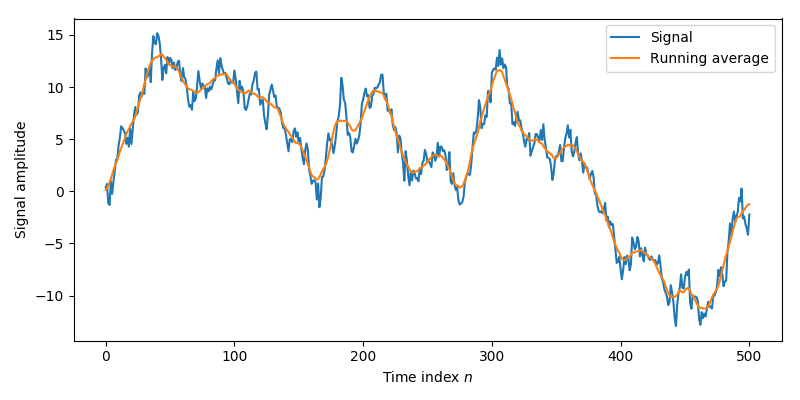
\includegraphics[width=\textwidth]{code/016_smoothing/smoothing.png}
  \end{center}
  \caption{A running average filter is often used to smooth a noisy
    signal. You can find the Python code used to produce this example
    in \texttt{016\_smoothing/smoothing.py}.}
  \label{fig:avg_filter}
\end{figure}

\section{Finite impulse response filter}
\begin{marginfigure}

\begin{center}
  \begin{tikzpicture}[node distance=3cm,auto,>=latex']
    \node [int] (a) {LTI};
    \node (b) [left of=a, coordinate] {a};
%    \node (c) [below=a,node distance=3cm] {a};

%\node [int, pin={[init]above:$p_0$}] (c) [right of=a] {$\frac{1}{s}$};
    \node [coordinate] (end) [right of=a]{};
    \path[->] (b) edge node {$x[n]$} (a);
    \path[->] (b) edge node [below]{$\delta[n]$} (a);

%\path[->] (a) edge node {$v$} (c);
    \draw[->] (a) edge node {$y[n]$} (end) ;
    \draw[->] (a) edge node [below]{$h[n]$} (end) ;

\end{tikzpicture}
\end{center}
\caption{Discrete-time LTI systems are characterized by an impulse response $h[n]$, which is the response of the LTI system to a unit impulse signal.}
\end{marginfigure}

The previous system shown in Equation \ref{eq:running_mean} is a special case of a more general type of discrete-time LTI system, 
known as a Finite Impulse Response (FIR) filter. This type of signal is often used in digital signal processing. 
An FIR filter is defined as follows:
\begin{equation}
  \boxed{
    y[n] = \sum_{k=-M}^{N} b_k x[n-k]\,\,.
  }
  \label{eq:fir_filter}
\end{equation}
The coefficients $b_k \in \mathbb{C}$ here are constant valued coefficients. As the name implies, there is a finite number of non-zero coefficients $b_k$. 
In the case of the running average filter in Equation \ref{eq:running_mean}, there would be 15 coefficients, which are all $b_k=1/15$.

\section{General discrete-time LTI system}
What if we allow there to be infinitely many coefficients for the system given in Equation \ref{eq:fir_filter}? We get the following:
\begin{equation}
    y[n] = \sum_{k=-\infty}^{\infty} b_k x[n-k] = \sum_{k=-\infty}^{\infty} b[k] x[n-k]\,\,.
\end{equation}
This turns out to be the general representation for arbitrary discrete-time LTI systems! In this case, it makes sense to think of the infinitely many coefficients $b_k$ as a signal $b[k]$.

For discrete-time LTI systems in general, the output of a system is given by a discrete-time convolution sum of the input signal $x[n]$ with an impulse response $h[n]$:

\begin{marginfigure}
  \begin{center}
          \begin{tikzpicture}
          \begin{axis}[width=7cm,height=4cm,ymin=0,xmin=-10,ymax=0.1,xmax=12,
         xtick={-10,-7,0,7,10},
              ytick={0,1,2,3},
              ytick={0,0.0667},
              yticklabel={,,},
          ylabel={$h[n]$},
      xlabel={$n$}, axis lines = center]
     \addplot+[ycomb,color=black] plot coordinates {(-10,0)(-9,0)(-8,0)(-7,0.0667)(-6,0.0667)(-5,0.0667)(-4,0.0667)(-3,0.0667)(-2,0.0667)(-1,0.0667)(0,0.0667)(1,0.0667)(2,0.0667)(3,0.0667)(4,0.0667)(5,0.0667)(6,0.0667)(7,0.0667)(8,0)(9,0)(10,0)};
  \end{axis}
  \end{tikzpicture}
  \end{center}
  \caption{The impulse response of the 15 point running mean filter described in Equation \ref{eq:running_mean}.}
\end{marginfigure}

\begin{equation}
  \boxed{
    y[n] = \mathcal{T}\{x[n]\}=\sum_{k=-\infty}^{\infty} h[k] x[n-k]\,\,.
  }
  \label{eq:conv_dlti}
\end{equation}
The impulse response is defined as follows:
\begin{equation}
  \boxed{
    h[n] = \mathcal{T}\{\delta[n]\}\,\,.
  \label{eq:conv_ireq}    
    }
\end{equation}
It is hopefully easy to see that Equation \ref{eq:conv_dlti} is valid for all LTI systems. %This was already briefly discussed earlier in the chapter on Fourier transforms.

A linear system $\mathcal{T}\{\cdot\}$\footnote{If linearity applies for two input signals $\mathcal{T}\{\alpha_1 s_1[n] + \alpha_2 s_2[n]\} = \alpha_1 \mathcal{T}\{s_1[n]\}+\alpha_2 \mathcal{T}\{s_2[n]\}$, it also applies for linear combinations of three or more signals.} must by definition satisfy the following relation:
\begin{equation}
  \mathcal{T}\left\{\sum_{k=-\infty}^{\infty} \alpha_k s_k[n]\right\} = \sum_{k=-\infty}^{\infty} \alpha_k \mathcal{T}\{s_k[n]\}\,\,.
  \label{eq:linearity_gen}
\end{equation}
Here $\alpha_k \in \mathbb{C}$ are arbitrary constants and $s_k[n]$ are arbitrary signals.

Time-invariance of $\mathcal{T}\{\cdot\}$, on the other hand, implies that for any time shift $k$ in the input, the output is correspondingly time shifted. 
This is valid for any input signal $x[n]$:
\begin{equation}
y[n-k] = \mathcal{T}\{x[n-k]\}\,\,,
\end{equation}
if 
\begin{equation}
y[n]=\mathcal{T}\{x[n]\}\,\,.
\end{equation}
It is possible to represent any signal $x[n]$ with the help of time-shifted unit impulse signals\sidenote{Recall that the discrete-time unit impulse is defined as: 
\begin{equation}
\delta[n] = \left\{
  \begin{array}{rcr}
    1 & \mathrm{when} & n=0 \\
    0 & \mathrm{otherwise} & \\
  \end{array}
\right.\,\,.
\end{equation}

It is the discrete-time equivalent of a Dirac delta function. The unit impulse is shown in Figure \ref{fig:dt_unit_impulse}.
}:
\begin{equation}
  x[n] = \sum_{k=-\infty}^{\infty} x[k]\delta[n-k]\,\,.
\end{equation}
Linearity implies that:
\begin{equation}
\mathcal{T}\{x[n]\} = \mathcal{T}\left\{\sum_{k=-\infty}^{\infty}x[k]\delta[n-k]\right\} = \sum_{k=-\infty}^{\infty}x[k] \mathcal{T}\{\delta[n-k]\}\,\,.
\end{equation}
\if 0
\begin{marginfigure}
\begin{center}
    \begin{tikzpicture}
      \begin{axis}[width=7cm,height=4cm,ymin=0,xmin=-10,ymax=0.1,xmax=12,
                   xtick={-10,-7,0,7,10},
                  ytick={0,1,2,3},
             ytick={0,0.0667},
             yticklabel={,,},
             ylabel={$h[n]$},
             xlabel={$n$}, axis lines = center]
        \addplot+[ycomb,color=black] plot coordinates {(-10,0)(-9,0)(-8,0)(-7,0.0667)(-6,0.0667)(-5,0.0667)(-4,0.0667)(-3,0.0667)(-2,0.0667)(-1,0.0667)(0,0.0667)(1,0.0667)(2,0.0667)(3,0.0667)(4,0.0667)(5,0.0667)(6,0.0667)(7,0.0667)(8,0)(9,0)(10,0)};
      \end{axis}
     \end{tikzpicture}
\end{center}
\caption{The impulse response of the 15 point running mean filter described in Equation \ref{eq:running_mean}.}
\end{marginfigure}
\fi
\noindent The equation above is the same as Equation \ref{eq:linearity_gen} with $s_k[n] = \delta[n-k]$ and $\alpha_k=x[k]$.  Due to time-invariance,
we can relate the impulse response $h[n]$ delayed by $k$ to the term
on the right-hand side above. If a unit impulse fed into the system is
\begin{equation}
h[n] = \mathcal{T}\{\delta[n]\},
\end{equation}
\begin{marginfigure}
  \begin{center}
    \begin{tikzpicture}
      \begin{axis}[width=7cm,height=4cm,ymin=0,xmin=-4,ymax=1.2,xmax=7,
                   xtick={-3,-2,-1,0,1,2,3,4,5,6},
                   ytick={0,1,2,3},
                   ylabel={$\delta[n]$},
                   xlabel={$n$}, axis lines = center]
          \addplot+[ycomb,color=black] plot coordinates {(-3,0) (-2,0) (-1,0) (0,1) (1,0) (2,0) (3,0) (4,0) (5,0) (6,0)};
      \end{axis}
     \end{tikzpicture}
     \begin{tikzpicture}
        \begin{axis}[width=7cm,height=4cm,ymin=0,xmin=-4,ymax=1.2,xmax=7,
          xtick={3},
          xticklabels={$n_0$},
          ytick={0,1,2,3},
          ylabel={$\delta[n-n_0]$},
          xlabel={$n$}, axis lines = center]
          \addplot+[ycomb,color=black] plot coordinates {(-3,0) (-2,0) (-1,0) (0,0) (1,0) (2,0) (3,1) (4,0) (5,0) (6,0)};
        \end{axis}
      \end{tikzpicture}
  \end{center}
  \caption{Discrete-time unit impulse signal $\delta[n]$ and a time-shifted version $\delta[n-n_0]$ centered at $n=n_0$.}
  \label{fig:dt_unit_impulse}
\end{marginfigure}
then a time-shifted unit impulse corresponds to a time-shifted output:
\begin{equation}
h[n-k] = \mathcal{T}\{\delta[n-k]\}\,\,.
\end{equation}
Therefore, the output of an LTI system for an arbitrary input signal
$x[n]$ can be expressed using the impulse response $h[n]$ as follows:
\begin{equation}
  y[n] = \sum_{k=-\infty}^{\infty} x[k]h[n-k].
  \label{eq:convolution_intro}
\end{equation}
This type of equation is known as a discrete-time convolution sum. We have now shown that any discrete-time LTI system can be represented with such a convolution sum. 
Note that Equation \ref{eq:convolution_intro} isn't quite yet the same as Equation \ref{eq:conv_dlti}. We will later show that the convolution sum is commutative, i.e., that:
\begin{equation}
 \sum_{k=-\infty}^{\infty} x[k]h[n-k] = \sum_{k=-\infty}^{\infty} h[k]x[n-k].
\end{equation}
Which completes the proof.

\subsection{Example: Impulse response of an FIR filter}
An FIR filter (Equation \ref{eq:fir_filter}) has the following impulse response:
\begin{equation}
h[n] = \sum_{k=-M}^{N} b_k \delta[n-k]\,\,.
\end{equation}
The signal $h[n]$ contains the values of the filter coefficients $h[n]=b_n$. Since there are a finite number of coefficients $b_k$, the impulse response $h[n]$ 
has non-zero values only in a finite range of samples. This is also where the name ``finite impulse response'' comes from.
\begin{marginfigure}
\begin{center}
  \begin{tikzpicture}[node distance=2cm,auto,>=latex']
    \node [int] (a) {FIR filter ($b_k$)};
    \node (b) [left of=a, coordinate] {a};
%    \node (c) [below=a,node distance=3cm] {a};

%\node [int, pin={[init]above:$p_0$}] (c) [right of=a] {$\frac{1}{s}$};
    \node [coordinate] (end) [right of=a]{};
    \path[->] (b) edge node {$\delta[n]$} (a);
    %\path[->] (a) edge node {$v$} (c);
    \draw[->] (a) edge node {$h[n]$} (end) ;
\end{tikzpicture}
\end{center}
\caption{The impulse response of an FIR filter is a signal that contains the coefficients. For a finite number of coefficients $b_k$, the length of 
the non-zero portion of the impulse response is finite, and hence the name FIR.}
\end{marginfigure}


\section{Impulse response}
Linear time-invariant (LTI) systems are fully characterized by an \index{impulse response} impulse response $h(t)$. 
This impulse response is obtained by feeding a unit impulse into the LTI system:
\begin{equation}
\boxed{
h(t) = \mathcal{T}\{\delta(t)\}\,\,.
}
\end{equation}
Using an impulse response, it is possible to represent the output of any LTI system as a convolution between the impulse response and the input signal.
\begin{equation}
\boxed{
y(t) = \mathcal{T}\{x(t)\} = h(t)*x(t) = \int_{-\infty}^{\infty} h(\tau)x(t-\tau)d\tau\,\,.
}
\end{equation}
Let's prove this. We'll first need to represent an arbitrary signal as a sum of unit impulses:
\begin{equation}
x(t)  = \int_{-\infty}^{\infty} x(\tau) \delta(t-\tau) d\tau\,\,.
\end{equation}
One way to think of this integral is that the unit impulse $\delta(t-\tau)$ ``selects'' the value of $x(\tau)$ where $\tau=t$. 
Another way to think of this is that the Dirac delta functions form a set of basis functions for representing the signal $x(t)$.

\tikzstyle{int}=[draw, minimum size=2em]
\tikzstyle{init} = [pin edge={to-,thin,black}]

\begin{marginfigure}
\begin{center}

  \begin{tikzpicture}[node distance=3cm,auto,>=latex']

    \node [int] (a) [align=center]{LTI };
    \node (b) [left of=a, coordinate] {a};
%    \node (c) [below=a,node distance=3cm] {a};

%\node [int, pin={[init]above:$p_0$}] (c) [right of=a] {$\frac{1}{s}$};
    \node [coordinate] (end) [right of=a]{};
    \path[->] (b) edge node {$\delta(t)$} (a);
  %  \path[->] (b) edge node [below]{$\delta(t)$} (a);

%\path[->] (a) edge node {$v$} (c);
    \draw[->] (a) edge node {$h(t)$} (end) ;
 %   \draw[->] (a) edge node [below]{$h(t)$} (end) ;

\end{tikzpicture}

\end{center}
\caption{A linear time-invariant system is characterized by an impulse response.}
\end{marginfigure}

You may recall that linearity of the system $\mathcal{T}\{\cdot\}$ implies that:
\begin{equation}
\mathcal{T}\{c_1 \delta(t-\tau_1) + c_2 \delta(t-\tau_2)\} = c_1 \mathcal{T}\{\delta(t-\tau_1)\}+ c_2 \mathcal{T}\{\delta(t-\tau_2)\}\,\,.
\end{equation}
Here I've used $\delta(t-\tau_1)$ and $\delta(t-\tau_2)$ as two different input signals. The terms $c_1,c_2\in \mathbb{C}$ are arbitrary complex-valued constants.

Linearity must therefore also apply for the linear combination of an arbitrary number of inputs:
\begin{equation}
\mathcal{T}\left\{\sum_n x_n \delta(t-\tau_n)\right\} = \sum_n x_n \mathcal{T}\{\delta(t-\tau_n)\}\,\,.
\end{equation}
Linearity can be extended even further into a continuous linear combination:
\begin{equation}
\mathcal{T}\left\{\int_{-\infty}^{\infty} x(\tau)\delta(t-\tau)d\tau\right\} = \int_{-\infty}^{\infty} x(\tau) \mathcal{T}\{\delta(t-\tau)\} d\tau\,\,.
\end{equation}
We can simplify the right-hand side and get:
\begin{equation}
\int_{-\infty}^{\infty} x(\tau) \mathcal{T}\{\delta(t-\tau)\} d\tau = \mathcal{T}\left\{x(t)\right\}\,\,.
\end{equation}
In order to simplify the left-hand side, we have to rely on the property of \emph{time-invariance}. That is:
\begin{equation}
h(t) = \mathcal{T}\{\delta(t)\} \Rightarrow h(t-\tau) = \mathcal{T}\{\delta(t-\tau)\}\,\,.
\end{equation}
This now completes our proof:
\begin{equation}
y(t)=\int_{-\infty}^{\infty} x(\tau) h(t-\tau) d\tau = \mathcal{T}\left\{x(t)\right\}\qed\,\,.
\end{equation}
The output of a linear time-invariant system $y(t)=\mathcal{T}\{x(t)\}$ is a convolution of the system's 
impulse response $h(t)=\mathcal{T}\{\delta(t)\}$ with the input signal $x(t)$ fed into the system.

\section{Convolution}

A convolution operation is defined for both continuous-time and
discrete-time signals. As we just saw, a convolution operation can be
interpreted as an LTI system applied to a signal.

The continuous-time convolution is defined as an integral:
\begin{equation}
\boxed{
  a(t)*b(t) = \int_{-\infty}^{\infty}a(\tau)b(t-\tau)d\tau\,\,.
}
\end{equation}
The discrete-time convolution is defined as a sum:
\begin{equation}
\boxed{
  a[n]*b[n] = \sum_{k=-\infty}^{\infty}a[k]b[n-k]\,\,.
}
\end{equation}

\section{Properties of a convolution}
The properties of the convolution operation are shown in Table \ref{con:table}. The same properties also exist for the continuous-time convolution
operation. 
\begin{table}
    \centering
    \caption{Table of convolution properties}
    \label{con:table}
    \begin{tabular}{|c|c|}
    \hline
    Property     & Equation \\ \hline
    identity     & $x[n]*\delta[n]=x[n]$ \\ \hline
    commutative  & $a[n] * b[n] = b[n] * a[n]$ \\ \hline
    associative  & $(a[n]*b[n]) * c[n] = a[n] * ( b[n] * c[n])$ \\ \hline
    distributive & $a[n]*(b[n]+c[n]) = a[n]*b[n] + a[n]*c[n]$ \\ \hline
    \end{tabular}
\end{table}

The proof of the identity property is clear, and the commutative property is left as an exercise. The associative property takes a bit more work, and the proof is as follows: 
\begin{proof}
Using the definition of the convolution operation twice:
\begin{align}
(a[n]*b[n])*c[n] &= \sum_{k}\underbrace{\left(\sum_\ell a[\ell]b[k-\ell]\right)}_{a[k]*b[k]} c[n-k] \\
                 &= \sum_{k}\sum_\ell a[\ell]b[k-\ell]c[n-k]
\end{align}
For the other ordering:
\begin{align}
a[n]*(b[n]*c[n]) &= \sum_{\ell} a[\ell] \Big(\underbrace{\sum_m b[m]c[(n-m)}_{b[n]*c[n]}-\ell]\Big)\\
                 &= \sum_{\ell} \sum_m a[\ell] b[m]c[(n-m)-\ell]\,\,.
\end{align}
If we now substitute: $m=k-\ell$, then $n-m-\ell=n-k$, which gives
\begin{align}
a[n]*(b[n]*c[n]) &= \sum_{k} \underbrace{\left(\sum_{\ell} a[\ell] b[k-\ell]\right)}_{a[k]*b[k]} c[n-k]\,\,,
\end{align}
which is the same as $(a[n]*b[n])*c[n]$, which completes the proof.
\end{proof}

\begin{marginfigure}
\begin{center}
  \begin{tikzpicture}[node distance=3cm,auto,>=latex']

    \node [int] (a) {LTI $(h_1[n])$};
    \node [above of=a, node distance=1cm] (in) {$x[n]$};
    \node [int, below of=a, node distance=1cm] (b) {LTI $(h_2[n])$};
    \node [below of=b, node distance=1cm] (out) {$y[n]$};
    \path[->] (a) -> (b);
    \draw[->] (a) -> (b);
    \path[->] (in) -> (a);
    \draw[->] (in) -> (a);
    \path[->] (b) -> (out);
    \draw[->] (b) -> (out);
    
    \node [int, right of=a,node distance=2cm] (a3) {LTI $(h_3[n])$};
    \node [above of=a3, node distance=1cm] (in3) {$x[n]$};
    \node [below of=a3, node distance=1cm] (out3) {$y[n]$};
    \path[->] (in3) -> (a3);
    \draw[->] (in3) -> (a3);
    \path[->] (a3) -> (out3);
    \draw[->] (a3) -> (out3);
    
\end{tikzpicture}
\end{center}
\caption{A consequence of the associative property of convolution is
  that two LTI systems characterized with $h_1[n]$ and $h_2[n]$ can be
  combined as a single LTI system with impulse response
  $h_3[n]=h_1[n]*h_2[n]$.}
\label{fig:cascade_lti1}
\end{marginfigure}

A consequence of the associative property is that if we have two LTI
systems that are applied to an input signal $x[n]$ in series, we can
come up with a single LTI system that is equivalent to two \index{chained 
LTI system} chained LTI systems:
\begin{equation}
  y[n] = (x[n]*h_1[n])*h_2[n] = x[n]*h_3[n]\,\,.
\end{equation}
Here $h_3[n]=h_1[n]*h_2[n]$. This is depicted in Figure
\ref{fig:cascade_lti1}. This property can be extended to an arbitrary
number of systems that are connected together in series.

\subsection{Distributive}

\begin{marginfigure}

\begin{center}
  \begin{tikzpicture}[node distance=3cm,auto,>=latex']

    \node [draw,shape=circle](p) {$+$};
    \node [int, above left of=p,node distance=1.5cm] (a1) {LTI $(h[n])$};
    \node [int, above right of=p,node distance=1.5cm] (a2) {LTI $(h[n])$};
    \node [above of=a1,node distance=1cm] (i1) {$x_1[n]$};
    \node [above of=a2,node distance=1cm] (i2) {$x_2[n]$};
    \node [below of=p,node distance=1cm] (o1) {$y[n]$};

    \path[->] (i1) -> (a1);
    \draw[->] (i1) -> (a1);
    \path[->] (i2) -> (a2);
    \draw[->] (i2) -> (a2);
    
    \path[->] (a1) -> (p);
    \draw[->] (a1) -> (p);
    \path[->] (a2) -> (p);
    \draw[->] (a2) -> (p);
    \path[->] (p) -> (o1);
    \draw[->] (p) -> (o1);
    
    
    \node [int, right of=a2,node distance=2cm] (a3) {LTI $(h[n])$};
    \node [above of=a3, node distance=1cm] (in3) {$x_1[n]+x_2[n]$};
    \node [below of=a3, node distance=1cm] (out3) {$y[n]$};
    \path[->] (in3) -> (a3);
    \draw[->] (in3) -> (a3);
    \path[->] (a3) -> (out3);
    \draw[->] (a3) -> (out3);
    
\end{tikzpicture}
\end{center}
\caption{A consequence of the distributive property is linearity.}
\label{fig:sum_lti}
\end{marginfigure}

The convolution is distributive:
\begin{equation}
a[n]*(b[n]+c[n]) = a[n]*b[n] + a[n]*c[n]\,\,.
\end{equation}

\begin{proof}
\begin{align}
a[n]*(b[n]+c[n]) & = \sum_{k=-\infty}^{\infty} a[k](b[n-k]+c[n-k]) \\
 & = \sum_{k=-\infty}^{\infty} a[k]b[n-k]+ \sum_{k=-\infty}^{\infty} a[k]c[n-k]\,\,.
\end{align}
\end{proof}

An example application of this property is shown in Figure
\ref{fig:sum_lti}. Signals $x_1[n]$ and $x_2[n]$ fed into an identical
LTI systems separately and then added together is equivalent to the
sum of the signals fed into a single LTI system.


\section{Example: Convolution animations}

Animations of the convolution operation for various example systems
can be found here: \url{http://kaira.uit.no/juha/fir_animation/}. The
code for creating such animations can be obtained from GitHub:
\url{https://github.com/jvierine/signal_processing/tree/master/017_fir_animation}.




\section{Applications of convolution}

This chapter only scratches the practical and theoretical uses of
convolution and linear time-invariant systems. I'll use two examples
to illustrate the application of a one-dimensional convolution
equation. Be aware that these are by no means the only types of
situations where you will encounter a convolution. Chances are quite
high that a signal processing system you can think of is an LTI
system, or can be approximated as one. Convolution can be found
everywhere!

\subsection{Example: Radar and sonar equation}

\begin{marginfigure}
\begin{center}
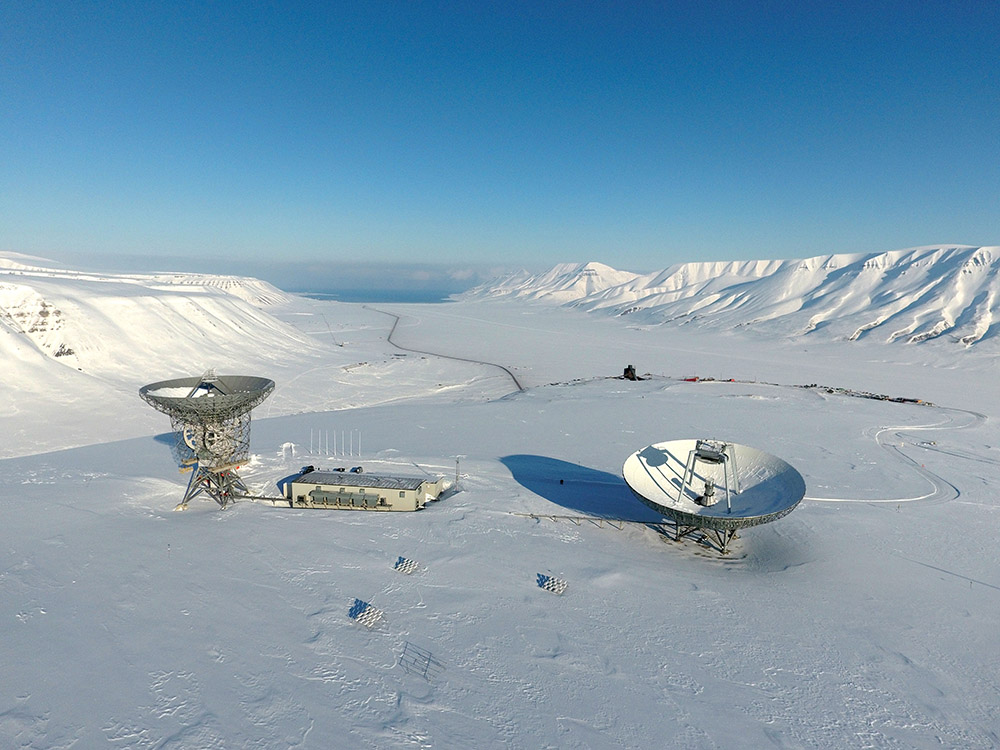
\includegraphics[width=\textwidth]{Applications/figures/svalbard.jpg}
\end{center}
\caption{EISCAT Svalbard Radar. The radar echo from the D-region of the ionosphere can be modeled using the equation shown in Equation \ref{eq:convolution_radar}. Photo: Craig Heinselman}
\label{fig:eiscat_svalbard}
\end{marginfigure}
The convolution equation is often used to model radar and sonar
measurements. In this case, the impulse response signal $h[n]$
represents the signal that is scattered as a function of distance. The
signal $x[n]$ represents what a radar or sonar transmits. The signal
received by a radar or sonar receiver $m[n]$ is then modeled as:
\begin{align}
m[n] &=  h[n]*x[n]\\
     &= \sum_{r=0}^{M} h[r] x[n-r]. \label{eq:convolution_radar}\,\,.
\end{align}
In this case, the index $r \in \mathbb{N}$ represents round-trip
propagation time between the transmitter and the receiver. The larger
the distance between the transmitter and the receiver, the larger the
delay. Assuming that the sample rate is $f_s$ in units of hertz or
($\frac{1}{\mathrm{s}}$), and the group velocity of the transmitter
wave $v_g$ ($\frac{\mathrm{m}}{\mathrm{s}}$), the round-trip range is given by:
\begin{equation}
R = \frac{v_g r}{2 f_s}\,\,.
\end{equation}
In the case of radar, the group velocity for electromagnetic waves is
$v_g \approx 3 \cdot 10^8$ ($\frac{\mathrm{m}}{\mathrm{s}}$). For sonar, it is the speed of
acoustic waves within the medium. In the case of air, this is
$v_g \approx 343$ ($\frac{\mathrm{m}}{\mathrm{s}}$).

To see how the convolution equation is the radar equation, we can use
an illustration, as shown in Figure \ref{fig:range_time_diagram}.
\begin{figure}
\begin{center}
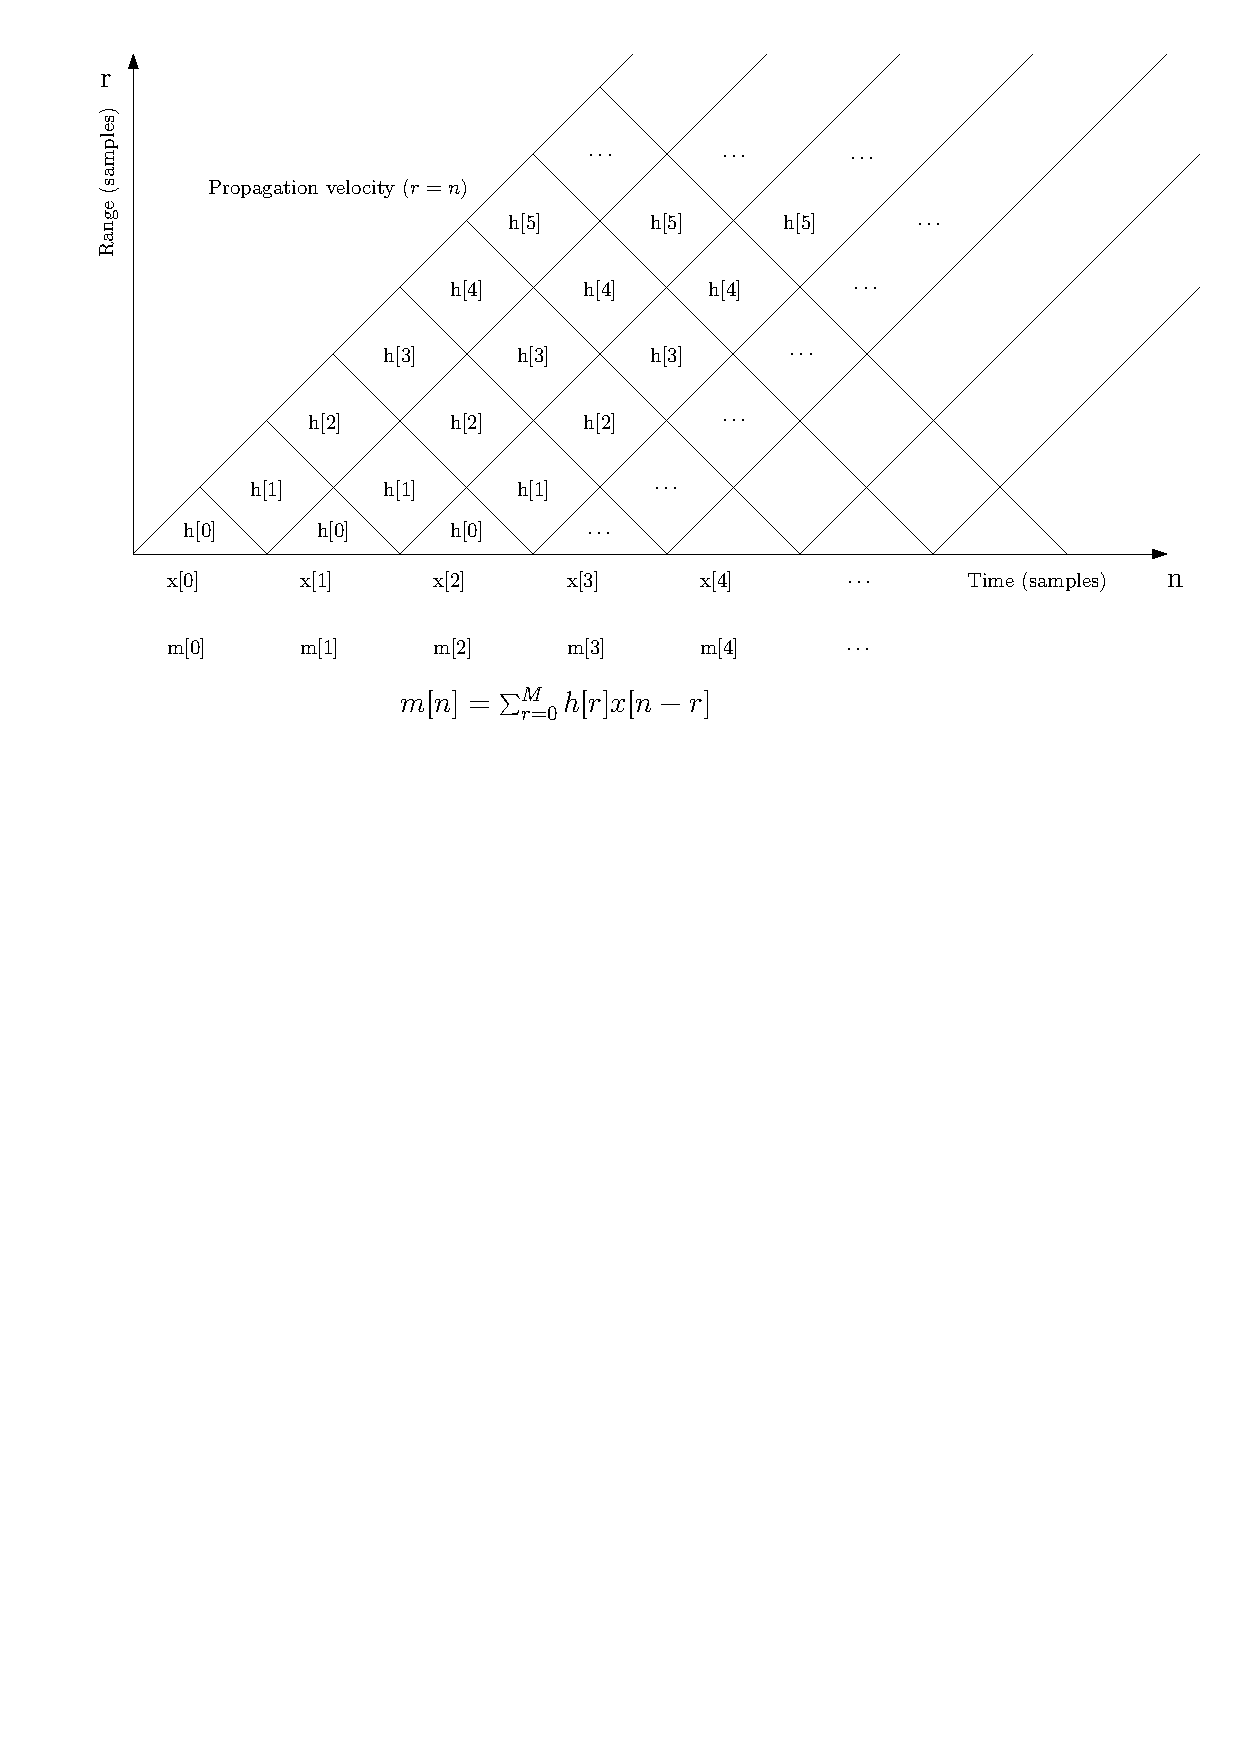
\includegraphics[width=\textwidth]{Applications/figures/rd.pdf}
\end{center}
\caption{A range-time diagram depicting the relationship between a transmitted signal and a scattered signal.}
\label{fig:range_time_diagram}
\end{figure}

If the probing signal is a unit impulse $x[n]=\delta[n]$ (a very short
radar pulse), then the measurement directly provides the scattering
amplitude as a function of range:
\begin{align}
m[n] = \sum_{r=0}^M h[r]\delta[n-r] = h[r]\,\,.
\end{align}
This type of radar is called a pulsed radar. In terms of radar
signal processing, this is the easiest case, as no signal processing
is needed! A radar measurement in this case is equivalent to measuring
the ``impulse response'' of the region that the radar is probing.

Here is a fascinating example of a blind child that has learned to
click his tongue (emitting a $\delta[n]$-like impulse sound) to probe the
acoustic scattering of his
surroundings \url{https://www.youtube.com/watch?v=fnH7AIwhpik}. While
this may seem like a superhuman feat, this is not unlike measuring the
distance between yourself and a mountain side by shouting ``echo''
very loudly and counting how long it takes for you to hear a strong
echo. I am sure that many of you have done this already.

\begin{marginfigure}
\begin{center}
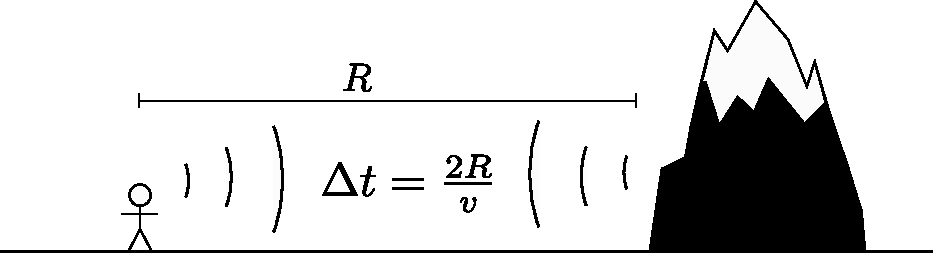
\includegraphics[width=\textwidth]{Applications/figures/mountain_echo.pdf}
\end{center}
\caption{The acoustics of a space are determined by acoustic waves
scattered from various obstacles at various propagation delays. This
can be quite precisely modeled using a convolution, assuming that
nothing is moving.}
\end{marginfigure}

If the transmitted waveform $x[n]$ is more complicated than a unit
impulse, the measurements need to be filtered in some way to
reconstruct the scattered signal as a function of range $h[n]$. This
is achieved by designing a filter $\lambda[n]$, which has the
following property $\lambda[n]*x[n] \approx \delta[n]$. After applying
the filter $\lambda[n]$ to the measured signal, one obtains the echo
as a function of range:
\begin{align}
\lambda[n]*m[n] = \lambda[n]*h[n]*x[n] = (\lambda[n]*x[n])*h[n]\approx h[n]\,\,. 
\end{align}
Design of pairs of signals $x[n]$ and filters $\lambda[n]$ is a topic
of radar signal processing. An example of a good pairing of a radar
transmit signal and a receiver filter is shown in the following convolution animation:
\url{http://kaira.uit.no/juha/fir_animation/ex12.gif}.
This is the so-called 13-bit Barker code and the inverse filter that
corresponds to it. The convolution of these two signals is the unit
impulse.
\section{Example: Reverb effect}
\label{reverb_section}

Convolution is encountered when modeling the acoustics of a room or a
space in audio signal processing. The basic underlying principle is
the same as for radar and sonar.

A sound source $x[n]$ is reflected or scattered from different
surfaces within the room at various delays $r$. Each delay $r$
corresponds to the round-trip propagation delay of the acoustic
signal. This is what creates the ``sound'' of a room. This is also
what is the cause for an acoustic ``echo'' from a mountain side that
you may have experienced in real life!

How much signal is scattered from range $r$ is determined by the impulse
response $h[r]$. The resulting signal is a convolution $m[n] = h[n]*
x[n]$. In this case, performing the convolution results in a reverb
effect in acoustic signal processing. 

By accurately modeling the impulse response of a room or a large
concert hall with an impulse response $h[n]$, it is possible to modify
an audio signal $x[n]$ to sound like it was played in that space.

\begin{marginfigure}
\begin{center}
\includegraphics[width=\textwidth]{Applications/figures/reverb.pdf}
\end{center}
\caption{An impulse response that models the acoustics of a large space, with echoes at up to 3 seconds time delay.}
\label{fig:room_model}
\end{marginfigure}


One way to characterize $h[n]$ for a room is to simply measure it. One
emits a very short discrete unit impulse $\delta[n]$ using a high
quality speaker, and then measures the echoes for this pulse to
obtain:
\begin{equation}
h[n] = \sum_{r=0}^M h[r]\delta[n-r]\,\,.
\end{equation}
Another possibility is to model the impulse response $h[n]$ by making
assumptions about the delays of the reflecting surfaces in a room or
space.

The following snippet of code demonstrates modeling of the acoustics
of a room using a modeled impulse response for a room.

\lstinputlisting[language=Python,caption={\texttt{018\_reverb/reverb.py}},label=lst:exercise_reverb]{code/018_reverb/reverb.py}
\newpage
\section{Exercises: Linear Time-invariant Systems}
\begin{enumerate}

\item Prove that the convolution operation is commutative. That is, show that $a[n]*b[n]=b[n]*a[n]$. In addition, show that this holds true for the continuous-time convolution operation. 

\item A running average system is defined as:
  \begin{equation}
    y[n] = \mathcal{T}\{x[n]\} = \frac{1}{L}\sum_{k=0}^{L-1} x[n-k]
  \end{equation}

  \begin{enumerate}[a)]
    \item Show that the running average system is a linear time
      invariant system using the test for linearity and time
      invariance.
    \item What is the impulse response $h[n] =
      \mathcal{T}\{\delta[n]\}$ of the running average system?
    \item How many non-zero values does the impulse response $h[n]$ have?
    \item We feed a discrete-time complex sinusoidal signal
      $x[n]=e^{i\hat{\omega}_0 n}$ into the system. Show that the
      output is of the form $y[n]=A e^{i\phi} e^{i\hat{\omega}_0 n}$,
      in other words, a discrete-time complex sinusoidal signal with
      the same frequency as the input signal.
      \item Continue with task d). Let us assume that
        $L=4$. What is the amplitude of the output signal $A$ when we
        have a normalized angular frequency of:
        \begin{enumerate}
        \item $\hat{\omega}_0 = 0$ radians per sample?
        \item $\hat{\omega}_0 = \pi$ radians per sample?
        \item $\hat{\omega}_0 = 0.5\pi$ radians per sample?          
        \end{enumerate}
      
    \item Show that system $y_2[n]=\mathcal{T}\{ \mathcal{T}\{x[n]\} \}$ is also an LTI system.
    \item What is the impulse response $h_2[n]=\mathcal{T}\{\mathcal{T}\{\delta[n]\}\}$? Sketch a plot of the non-zero values $h_2[n]$.
  \end{enumerate}
  
  \item Obtain the demonstration code that implements a reverb effect
    using a convolution operation:
    \begin{equation}
      y[n]=h[n]*x[n],
      \end{equation}
    where $x[n]$ is the input signal, $h[n]$ is the impulse response
    of a room, and $y[n]$ is the output signal with the reverb
    effect. Download \verb|7na.wav| from the course GitHub examples,
    \url{https://github.com/jvierine/signal_processing/tree/master/018_reverb}
    or alternatively use your own audio file.

\begin{enumerate}[a)]

\item Run the example code and verify that the filtered signal indeed sounds like it
is played in a large room by playing \verb|7na.wav| and the file \verb|reverb.wav|
produced by the script.

\item Find the part in the code where a convolution between the audio
  signal and the impulse response is evaluated. Plot the impulse
  response of the FIR filter applied to the input signal.

\item Figure out how to increase and reduce the amount of reverb, i.e.,
to make it sound like the audio signal is played in a large or small
room with many surfaces that reflect sound waves. What does the
impulse response for a large room and a small room look like?

\item Now try to create an impulse response of an echo from a distance
  of 1000 meters using the following impulse response
  $h[n]=\delta[n]+0.5\delta[n-n_0]$. Assuming that the propagation velocity of
  sound is 343 $\frac{\mathrm{m}}{\mathrm{s}}$, determine a suitable value for $n_0$.

\item Implement several length running average filters to
  the audio signal (e.g., Equation \ref{eq:running_mean}), which
  average together 4, 8, 16, and 100 samples. Can you detect
  with your ear what happens to the low and high frequency components
  of the signal as a result of the operation?
\end{enumerate}


\end{enumerate}
 \ifSpExerciseSol
 \newpage
\section{Suggested solutions: Linear Time-invariant Systems}
\begin{enumerate}

\item Claim: $a[n]*b[n]=b[n]*a[n]$.
\begin{proof}
By definition, the convolution of two discrete-time signals is defined as:
\begin{align*}
    a[n]*b[n]&=\sum_{k=-\infty}^{\infty} a[k]b[n-k].
\end{align*}
Change variables by setting $l=n-k$, so that $k=n-l$, then:
\begin{align*}
    a[n]*b[n]&=\sum_{l=-\infty}^{\infty}a[n-l]b[l]=\sum_{l=-\infty}^{\infty}b[l]a[n-l].
\end{align*}
The last sum is the definition of $b[n]*a[n]$, just with the sum index named $l$, hence $a[n]*b[n]=b[n]*a[n]$. 
\end{proof}
The same approach can be used to prove the commutativity of the continuous-time convolution. Again, substitution of variables, but with integrals. Here is the proof:
\begin{proof}
\begin{align*}
    a(t)*b(t) &= \int_{-\infty}^{\infty}a(\tau)b(t-\tau)d\tau, \\
              &= -\int_{\infty}^{-\infty}a(t-u)b(u)du, \\
              &= \int_{-\infty}^{\infty}b(u)a(t-u)du, \\
              &= b(t) * a(t),
\end{align*}
\end{proof}
where $u=t-\tau$, giving $du=-d\tau$. Note that the minus sign is used to swap the limits. 

\item Consider the running average system, defined as:
$$y[n]=\mathcal{T}\{x[n]\}=\frac{1}{L}\sum_{k=0}^{L-1}x[n-k].$$

\begin{enumerate}[a)]
\item Consider two discrete-time signals $x_{1}[n]$ and $x_{2}[n]$ with arbitrary constants $c_{1},c_{2}$, then:
\begin{align*}
    \mathcal{T}\{c_{1}x_{1}[n]+c_{2}x_{2}[n]\}&=\frac{1}{L}\sum_{j=0}^{L-1}[c_{1}x_{1}[n-j]+c_{2}x_{2}[n-j]], \\
    c_{1}\mathcal{T}\{x_{1}[n]\}+c_{2}\mathcal{T}\{x_{2}[n]\}&=c_{1}\frac{1}{L}\sum_{k=0}^{L-1}x_{1}[n-k]+c_{2}\frac{1}{L}\sum_{l=0}^{L-1}x_{1}[n-l],
\end{align*}
which are equal. 

For time-invariance we have:
\begin{align*}
    \mathcal{T}\{\mathcal{D}\{x[n]\}\}&=\mathcal{T}\{x[n-\tau]\}=\frac{1}{L}\sum_{k=0}^{L-1}x[n-\tau-k], \\
    \mathcal{D}\{\mathcal{T}\{x[n]\}\}&=\mathcal{D}\left\{\frac{1}{L}\sum_{k=0}^{L-1}x[n-k]\right\}=\frac{1}{L}\sum_{k=0}^{L-1}x[n-\tau-k],
\end{align*}
both are equal, so the system is time-invariant. 

\item The impulse response can be determined by $h[n]=\mathcal{T}\{\delta[n]\}$, doing this yields:
$$h[n]=\frac{1}{L}\sum_{k=0}^{L-1}\delta[n-k].$$
The impulse response function is then:
$$h[n]=\begin{cases}
    \frac{1}{L}, \quad n=0,\hdots,L-1, \\
    0, \quad \text{otherwise}.
\end{cases}$$

\item The impulse response has $L$ nonzero values, all of them being $1/L$. 

\item Let $x[n]=e^{i\hat{\omega}_{0}n}$, then if we feed this into our system we get:
$$y[n]=\frac{1}{L}\sum_{k=0}^{L-1}e^{i\hat{\omega}_{0}(n-k)}=\frac{1}{L}e^{i\hat{\omega}_{0}n}\sum_{k=0}^{L-1}e^{-i\hat{\omega}_{0}k}=\frac{1}{L}e^{i\hat{\omega}_{0}n}\left(\frac{1-(e^{-i\hat{\omega}_{0}})^{L}}{1-e^{-i\hat{\omega}_{0}}}\right).$$
The output signal is of the form $Ae^{i\phi}e^{i\hat{\omega}_{0}n}$ as $y[n]$ is then:
$$y[n]=\frac{1}{L}\frac{1-e^{-i\hat{\omega}_{0}L}}{1-e^{-i\hat{\omega}_{0}}}e^{i\hat{\omega}_{0}n}=\frac{1}{L}\frac{1-e^{-i\hat{\omega}_{0}L}}{1-e^{-i\hat{\omega}_{0}}}e^{i\hat{\omega}_{0}n}.$$

\item Take $L=4$, then:
$$y[n]=\frac{1}{4}\frac{1-e^{-i\hat{4\omega}_{0}}}{1-e^{-i\hat{\omega}_{0}}}x[n].$$
Next, consider the cases of input frequencies:
\begin{align*}
    \hat{\omega}&=0,\\
    \hat{\omega}&=\pi,\\
    \hat{\omega}&=0.5\pi,
\end{align*}
in these cases the amplitude of the output is:
\begin{align*}
    A&=\lim_{\hat{\omega}\to 0}\frac{1}{4}\frac{1-e^{-4i\hat{\omega}_{0}}}{1-e^{-i\hat{\omega}_{0}}}=\lim_{\hat{\omega}\to 0}\frac{1}{4}\frac{4ie^{-4i\hat{\omega}_{0}}}{ie^{-i\hat{\omega}_{0}}}=1, \\
    A&=\frac{1}{4}\frac{1-e^{-4i\pi}}{1-e^{-i\pi}}=0,\\
    A&=\frac{1}{4}\frac{1-e^{-4i\pi/2}}{1-e^{-i\pi/2}}=0.
\end{align*}

\item The system $y[n]=\mathcal{T}\{x[n]\}$ is an LTI system and can be written as $y[n]=h[n]*x[n]$, where $h[n]$ is the impulse response function as defined above. 
Then the system can be described as:
$$y_{2}[n]=\mathcal{T}\{\mathcal{T}\{x[n]\}\}=\mathcal{T}\{h[n]*x[n]\}=h[n]*(h[n]*x[n])=(h[n]*h[n])*x[n].$$
We've used associativity of convolution in the final step. Then the system can be described as $y_{2}[n]=h_{2}[n]*x[n]$, 
where $h_{2}[n]=h[n]*h[n]$. Hence, $y_{2}[n]$ is an LTI system, as all LTI system are fully determined by convolution with an impulse response. 

\item Have that $h_{2}[n]=\mathcal{T}\{\mathcal{T}\{\delta[n]\}\}=h[n]*h[n]$, so:
$$h_{2}[n]=\sum_{k=-\infty}^{\infty} h[k]h[n-k]=h[0]h[n]+h[1]h[n-1]+h[2]h[n-2]+h[3]h[n-3]+h[4]h[n-4].$$
Terms with $n<0$ are dropped as these will be $0$ due to $h[n]=0$ for $n<0$. Let's evaluate the values of $h_{2}[n]$ with $L=4$:
\begin{align*}
    h_{2}[0]&=h[0]h[0]+h[1]h[-1]+h[2]h[-2]+h[3]h[-3]+h[4]h[-4] = \frac{1}{L^{2}}, \\
    h_{2}[1]&=h[0]h[1]+h[1]h[0]+h[2]h[-1]+h[3]h[-2]+h[4][-3] =\frac{2}{L^{2}}, \\
    h_{2}[2]&=h[0]h[2]+h[1]h[1]+h[2]h[0]+h[3]h[-1]+h[4]h[-2] = \frac{3}{L^{2}}, \\
    h_{2}[3]&=h[0]h[3]+h[1]h[2]+h[2]h[1]+h[3]h[0]+h[4]h[-1] = \frac{4}{L^{2}}, \\
    h_{2}[4]&=h[0]h[4]+h[1]h[3]+h[2]h[2]+h[3]h[1]+h[4]h[0] = \frac{3}{L^{2}}, \\
    h_{2}[5]&=h[0]h[5]+h[1]h[4]+h[2]h[3]+h[3]h[2]+h[4]h[1] = \frac{2}{L^{2}}, \\
    h_{2}[6]&=h[0]h[6]+h[1]h[5]+h[2]h[4]+h[3]h[3]+h[4]h[2] = \frac{1}{L^{2}},
\end{align*}
while the rest are $0$. Thus:
$$h_{2}[n]=\begin{cases}
    \frac{1}{16}, \quad n=0,6,\\
    \frac{2}{16}, \quad n=1,5,\\
    \frac{3}{16}, \quad n=2,4,\\
    \frac{4}{16}, \quad n=3,\\
    0, \quad \text{otherwise}.
\end{cases}$$

To draw the impulse response function, we write a little program to do it. 
The program is shown in Listing \ref{code12_1}. The impulse response is $0$ for all values of $n$ not shown. 
\lstinputlisting[language=Python, caption=Simple convolution,label=code12_1]{ch10/code/ex10_2g.py}
The output of the program is shown in Figure \ref{h2}.

\begin{marginfigure}
    \includegraphics[width=7.5cm,height=6.5cm]{ch10/figures/h2.png}
    \caption{Impulse response for $y_{2}[n]$}
    \label{h2}
\end{marginfigure}
\end{enumerate}

\item Consider the reverb model as shown in Listing \ref{reverb:solution}.
\begin{enumerate}[a)]
    \item By running \verb|reverb.py| and listening to \verb|reverb.wav|, one can 
    hear the reverb effect having been applied to the audio-signal.
    
    \item Running the code yields the figure shown in Figure \ref{reverb:audio}.
    \begin{marginfigure}
    \includegraphics[width=7.5cm,height=7.0cm]{ch10/figures/reverb_impulse.png}
    \caption{Impulse response for the reverb LTI system}
    \label{reverb:audio}
    \end{marginfigure}
    
    \item By changing the \verb|room_length_std| and number of \verb|n_walls| one can get the 
    effect of a small room or a large one. If one increases \verb|room_length_std| the 
    room would be bigger as the echo have to travel further. The impulse response is similar, 
    but the impulse response for a larger room has more peaks at higher times. 
    
    \item To determine $n_{0}$, first consider the time it takes the echo to travel 
    1000 meters and then return. Have that $s=vt$, so $t=s/v$, assuming that 
    the speed is constant throughout. This means that, to travel back and forth takes:
    $$t=\frac{2s}{v}$$
    seconds. The total time in a discrete-time signal is $t=n_{0}T_{s}$, therefore:
    $$n_{0}=\frac{2s}{vT_{s}}=\frac{2sf_{s}}{v},$$
    where $f_{s}$ is the sample length, $s$ is the distance to the surface to scatter 
    from and $v$ is the speed of sound in the corresponding medium. Thus, for an 
    audio-signal sampled at $44100$ Hz, the delay index should be:
    $$n_{0}=\frac{2sf_s}{v}=\frac{(2)(1000\ \text{m})(44100)\ \text{Hz}}{343\ \text{m/s}}\approx257142.85,$$
    or $n_{0}=257143$ to round to the nearest integer. Implementing this with the \verb|reverb.py| 
    script can be accomplished by setting \verb|room_length_std| as 1000, 
    then \verb|n_walls| as 1, \verb|c_sound| as 343 and \verb|sr| as 44100.
    
    \item The average running filter can be implemented by setting the impulse 
    response as $h[n]=\frac{1}{M}\sum_k \delta[n-k]$. The effect on the audio is 
    that the high frequencies are reduced, as expected since the average running filter is a low-pass filter. 

    \lstinputlisting[language=Python,caption=Solution for exercise 3,label=reverb:solution]{ch10/code/ex10_3.py}

\end{enumerate}
\end{enumerate}
 \fi
\fi

\ifSpFResp
\chapter{Frequency Response}
In this chapter, we will investigate the response of an LTI system to
a complex sinusoidal input. This investigation leads to the concept
of \emph{\index{frequency response}{frequency response}} of an LTI
system. The frequency response allows you to determine how an LTI
system modifies each frequency component of a signal fed into the
system.

\begin{marginfigure}
    \tikzstyle{int}=[draw, minimum size=2em]
    \tikzstyle{init} = [pin edge={to-,thin,black}]
    \begin{center}

        \begin{tikzpicture}[every text node part/.style={align=center},node distance=3cm,auto,>=latex']
            %    \node [int] (a) {C-to-D \\ $T_s$};
            %  \begin{tikzpicture}[node distance=3cm,auto,>=latex']
            \node [int] (a) {LTI \\ $h(t)$};
            \node (b) [left of=a, coordinate] {a};
            \node [coordinate] (end) [right of=a]{};
            \path[->] (b) edge node {$x(t)=A e^{i \phi} e^{i \omega t}$} (a);
            \draw[->] (a) edge node {$y(t)=\mathcal{H}(\omega) x(t) $} (end) ;
        \end{tikzpicture}
    \end{center}
    \caption{The frequency response of a continuous-time LTI system is obtained
        by investigating what the system does to a complex sinusoidal signal.}
\end{marginfigure}

Every LTI system $\mathcal{T}\{\cdot\}$ can be expressed as a
convolution of an input signal $x(t)$ with the impulse response $h(t)=\mathcal{T}\{\delta(t)\}$
of the LTI system:
\begin{align}
    y(t) & = \mathcal{T}\{x(t)\}                                  \\
         & = x(t)*h(t)                                            \\
         & =\int_{-\infty}^{\infty} h(\tau) x(t-\tau) d\tau \,\,.
\end{align}
If we feed a complex sinusoidal signal $x(t)=Ae^{i\phi}e^{i\omega t}$
to an LTI system, we get\sidenote{
An \emph{\index{eigenfunction}{eigenfunction}} $x(t)$ of an operator
$\mathcal{T}\{\cdot\}$ is defined as a function that has the following property:
\begin{equation}
    \mathcal{T}\{x(t)\} = \lambda x(t) \,\,,
\end{equation}
where $\lambda \in \mathbb{C}$ is a constant. This means that applying
an operator on an eigenfunction of that operator is equivalent to
multiplication of this eigenfunction by a constant.

%This, combined with the fact that we can  is
%mathematically a very useful property, as it provides a powerful for
%studying what an operator does.

The derivation leading up to Equation \ref{eq:eig_ct} shows
that complex sinusoidal signals $x(t)=Ae^{i\phi}e^{i \omega t}$ are
eigenfunctions of LTI systems. The same property also applies
to discrete-time LTI systems and discrete-time complex sinusoidal signals.
}:
\begin{align}
    y(t) & = \int_{-\infty}^{\infty} h(\tau)x(t-\tau) d\tau                                                                                                        \\
         & = \int_{-\infty}^{\infty} h(\tau) A e^{i\phi} e^{i\omega(t-\tau)}  d\tau                                                                                \\
         & = \int_{-\infty}^{\infty}h(\tau) e^{-i \omega \tau} A e^{i\phi} e^{i \omega t } d\tau                                                                   \\
         & = \underbrace{\left(\int_{-\infty}^{\infty} h(\tau) e^{-i \omega \tau} d\tau\right)}_{\Hew} \underbrace{\left(A e^{i\phi} e^{i \omega t}\right)}_{x(t)} \\
         & = \Hew x(t) \,\,. \label{eq:eig_ct}
\end{align}
The output of the system is the input signal, multiplied by a complex
function $\Hew \in \mathbb{C}$, which depends on the angular frequency
$\omega$ of the input signal. The term $\Hew$ is called the frequency
response of the LTI system:
\begin{equation}
    \boxed{
        \Hew = \int_{-\infty}^{\infty} h(\tau) e^{-i \omega \tau} d\tau
    } \,\,.
    \label{eq:fresp_ct}
\end{equation}
From the definition, we can see that it is the same thing as a Fourier
transform of the impulse response $h(t)$.

\section{Arbitrary signals}

Let's consider an arbitrary continuous-time signal that is represented
as a sum\footnote{You can think of the inverse Fourier transform as stating
    that the signal $x(t)$ consists of a linear combination of infinitely many
    complex sinusoidal signals.} of complex sinusoidal signals using the inverse Fourier transform:
\begin{equation}
    x(t)  = \frac{1}{2\pi} \int_{-\infty}^{\infty} \hat{x}(\omega) e^{i \omega t} d\omega \,\,.
\end{equation}
Here $\hat{x}(\omega)$ is the Fourier transform of $x(t)$ -- it
represents the complex amplitude of spectral components of the signal
as a function of angular frequency $\omega$.

The convolution theorem\footnote{the convolution theorem was discussed
    in the continuous-time Fourier transform chapter} states that
convolution in time domain is multiplication in frequency domain:
\begin{equation}
    \boxed{
        y(t) = h(t)*x(t) \xleftrightarrow{\mathcal{F}} \hat{y}(\omega)=\mathcal{H}(\omega)\hat{x}(\omega)
    } \,\,.
\end{equation}
The frequency response therefore tells us how each frequency component
of the input signal is modified by the LTI system. Therefore, we can
view an LTI system as a filter. How each frequency component of the input
signal is modified, is determined by the Fourier transform of the impulse
response of the LTI system, which we will call \index{frequency response}
frequency response $\Hiw$.


\if 0
    This means that the signal fed through an LTI system has the following spectral representation:
    \begin{align}
        y(t) & = \frac{1}{2\pi} \int_{-\infty}^{\infty} \hat{y}(\omega) e^{i \omega t} d\omega                          \\
             & = \frac{1}{2\pi} \int_{-\infty}^{\infty} \mathcal{H}(\omega)\hat{x}(\omega) e^{i \omega t} d\omega \,\,.
    \end{align}
    This means that the LTI system modifies the frequency domain representation
    $\hat{x}(\omega)$ in such a way that the new representation is given by:
    \begin{equation}
        \boxed{
            \hat{y}(\omega) = \mathcal{H}(\omega)\hat{x}(\omega)
        } \,\,.
    \end{equation}
\fi


\section{Discrete-time frequency response}

A discrete-time LTI system $\mathcal{T}\{\cdot\}$ is also described by
a convolution of the input signal with the impulse response $h[n]$ of
the LTI system:
\begin{marginfigure}[-5cm]
    \tikzstyle{int}=[draw, minimum size=2em]
    \tikzstyle{init} = [pin edge={to-,thin,black}]
    \begin{center}
        \begin{tikzpicture}[every text node part/.style={align=center},node distance=3cm,auto,>=latex']
            %\begin{tikzpicture}[node distance=3cm,auto,>=latex']
            \node [int] (a) {LTI \\ $h[n]$};
            \node (b) [left of=a, coordinate] {a};
            %    \node (c) [below=a,node distance=3cm] {a};

            %\node [int, pin={[init]above:$p_0$}] (c) [right of=a] {$\frac{1}{s}$};
            \node [coordinate] (end) [right of=a]{};
            \path[->] (b) edge node {$A e^{i \phi} e^{i\hat{\omega} n}$} (a);
            %\path[->] (a) edge node {$v$} (c);
            \draw[->] (a) edge node {$\mathcal{H}(\hat{\omega})A e^{i \phi} e^{i\hat{\omega} n}$} (end) ;
        \end{tikzpicture}
    \end{center}
    \caption{The frequency response of a discrete-time LTI system is obtained by
        investigating what the system does to a complex sinusoidal signal.}
\end{marginfigure}
\begin{align}
    y[n] & = \mathcal{T}\{x[n]\}                         \\
         & =x[n]*h[n]                                    \\
         & = \sum_{k=-\infty}^{\infty} h[k] x[n-k] \,\,.
\end{align}
When inspecting the case where the input is a complex sinusoidal
signal $x[n]=Ae^{i\phi}e^{i\hat{\omega}n}$, with a normalized angular
frequency $\hat{\omega}$ and phase $\phi$, we get\sidenote[][-3cm]{The
    normalized angular frequency is defined as $\hat{\omega}=\omega T_s$
    (radians per sample), where $T_s$ (seconds) is the sample spacing, and
    $\omega$ is the continuous-time angular frequency (radians per
    second). Remember that it is possible to convert normalized angular
    frequency to frequency in units of cycles per second using the formula
    $\omega=2\pi f$. Which results in $f = \hat{\omega} f_s / 2\pi$, where
    the sample-rate is $f_s=1/T_s$. For example. this means that
    $\hat{\omega}=\pi$ corresponds to a frequency $f=f_s/2$.}:
\begin{align}
    y[n] & = \sum_{k} h[k]x[n-k]                                                                                                               \\
         & = \sum_{k} h[k] A e^{i\phi} e^{i\hat{\omega}(n-k)}                                                                                  \\
         & = \sum_{k} h[k] e^{-i\hat{\omega}k} A e^{i\phi} e^{i\hat{\omega}n}                                                                  \\
         & = \underbrace{\left(\sum_{k} h[k] e^{-i\hat{\omega}k}\right)}_{\He} \underbrace{\left(A e^{i\phi} e^{i\hat{\omega}n}\right)}_{x[n]} \\
         & = \He x[n] \,\,. \label{eq:eig_dt}
\end{align}
Here the complex-valued function $\He \in \mathbb{C}$, denotes
the \emph{discrete-time frequency response}, which is defined as:
\begin{equation}
    \boxed{
    \He = \sum_{k=-\infty}^{\infty} h[k]e^{-i\hat{\omega}k}
    } \,\, _.
    \label{eq:dt_fr}
\end{equation}
We'll later on show that this is a Fourier transform,
the \emph{discrete-time Fourier transform} of a discrete-time signal
$h[n]$. %All of the properties of a discrete-time Fourier transform
%also apply to $\He$.

%In this chapter, we'll mostly focus on the frequency response of
%discrete-time systems, but we will occasionally describe connections
%to continuous-time systems.


%\newpage
\begin{marginfigure}
    \begin{center}
        \begin{tikzpicture}
            \begin{axis}[axis equal, ymin=-0.5,xmin=-0.5,ymax=1.8,xmax=1.8,  ticks=none,
                    xlabel=$\mathrm{Re}$,
                    ylabel=$\mathrm{Im}$, axis lines = center, width=7cm, height=7cm]

                \addplot [gray,domain=0:2*pi,samples=50]({1.5*cos(deg(x))},{1.5*sin(deg(x))});

                \addplot [black, mark = *] coordinates {( {1.5*cos(45)}, {1.5*sin(45)} )} {};
                %   \addplot [black, mark = *] coordinates {( {1.5*cos(-60)}, {1.5*sin(-60)} )} {};   

                \addplot [black] coordinates { (0,0) ( {1.5*cos(45)}, {1.5*sin(45)} ) };

                \addplot [dashed,black] coordinates { ({1.5*cos(45)},0) ( {1.5*cos(45)}, {1.5*sin(45)} ) };

                \addplot [dashed,black] coordinates { (0,{1.5*sin(45)}) ( {1.5*cos(45)}, {1.5*sin(45)} ) };

                \draw[draw=black] (axis cs:0.2,0) arc [radius={transformdirectionx(0.2)},start angle=0,end angle=45]
                node[midway,right,inner sep=3pt,font={\footnotesize}]{$\angle \He$};

                \node at (axis cs:0.55,1.06) [above, font={\footnotesize}]{$\mathrm{Re}\{\He\}$};

                \node at (axis cs:1.1,0.65) [right, font={\footnotesize}]{$\mathrm{Im}\{\He\}$};

                \node at (axis cs:1.2,1.2) {$\He$};

                \node at (axis cs:0.5,0.5) [above,rotate=45,font={\footnotesize}]{$|\He|$};
            \end{axis}
        \end{tikzpicture}
    \end{center}
    \caption{The frequency response is complex-valued, and it represents a phase
        shift $\angle \He$ and a magnitude scaling $|\He|$ introduced by the LTI
        system to a complex sinusoidal signal of normalized angular frequency $\hat{\omega}$.}
    \label{fig:polar_he}
\end{marginfigure}


\section{Magnitude and phase response}
The frequency response $\He \in \mathbb{C}$ is a complex-valued
function. It can be expressed in either Cartesian or polar form
using Euler's formula:
\begin{equation}
    \He = \mathrm{Re}\left\{\He \right\} + i\mathrm{Im}\left\{\He \right\} = \left|\He\right|e^{i \angle \He } \,\,.
\end{equation}
This is shown in Figure \ref{fig:polar_he}.


When an LTI system is applied to a complex sinusoidal signal
$x[n]=Ae^{i\phi}e^{i\hat{\omega}n}$, the effect is scaling the
absolute value and shifting the phase of this signal:
\begin{align}
    y[n] & = x[n]*h[n]                                                                                        \\
         & = \He A e^{i\phi}e^{i\hat{\omega}n}                                                                \\
         & = \underbrace{(A|\He|)}_{A'}\underbrace{e^{i(\phi + \angle \He)}}_{e^{i\phi'}} e^{i\hat{\omega} n} \\
         & = A' e^{i\phi'} e^{i\hat{\omega} n} \,\,.
\end{align}
\begin{marginfigure}
    \begin{center}
        \begin{tikzpicture}
            \begin{axis}[width=6cm,height=4cm,domain=(-3.14):(3.14),samples=200, xmin=-4,xmax=4, ymin=0,ymax=1.2,
                    legend style={draw=none,at={(.99,.1)},anchor=south east},
                    xlabel={$\hat{\omega}$},
                    ylabel={$|\He|$},
                    axis x line=center,
                    axis y line=middle,
                    xtick={-3.14,0,3.14},
                    xticklabels={$-\pi$,0,$\pi$}
                ]
                \addplot[blue] {0.75+0.25*cos(deg(x))};
            \end{axis}
        \end{tikzpicture}
        \begin{tikzpicture}
            \begin{axis}[width=6cm,height=4cm,domain=(-3.14):(3.14),samples=200, xmin=-4,xmax=4, ymin=-3.3,ymax=3.3,
                    legend style={draw=none,at={(.99,.1)},anchor=south east},
                    xlabel={$\hat{\omega}$},
                    ylabel={$\angle \He$},
                    axis x line=center,
                    axis y line=middle,
                    xtick={-3.14,0,3.14},
                    xticklabels={$-\pi$,0,$\pi$}
                ]
                \addplot[blue] {-x};
            \end{axis}
        \end{tikzpicture}
    \end{center}
    \caption{An example frequency response. Top: The magnitude response of
        the LTI system $|\He|$. Bottom: The phase response of the system $\angle \He$.}
    \label{fig:he_example_lpf}
\end{marginfigure}

The output signal is still a complex sinusoidal signal with the same
frequency, but the amplitude $A$ is scaled by a factor of $|\He|$, and the
phase is shifted by a factor $\angle \He$. The magnitude of the
frequency response $|\He|$ is called the \emph{\index{magnitude
        response}{magnitude response}}:
\begin{equation}
    \boxed{
        |\He|=\sqrt{\Re\{\He\}^2+\Im\{\He\}^2}
    } \,\,,
\end{equation}
and the phase $\angle \He$ is called
the \emph{\index{phase response}{phase response}}
\begin{equation}
    \boxed{
        \angle \He = \tan^{-1}\left(\frac{\Im\{\He\}}{\Re\{\He\}}\right)
    } \,\,.
\end{equation}
of the LTI system.

Figure \ref{fig:he_example_lpf} shows an example frequency response
for a low-pass filter, which reduces the absolute value of complex
sinusoidal signals with high frequencies near
$\hat{\omega}=\pm \pi$. The filter also introduces a phase shift,
which is described by a linear slope. We'll later see that a linear
slope means that the system applies a time-shift to the input signal.

%\newpage
\section{Example: Low-pass filter}

Let's find the frequency response of the finite impulse response (FIR)
filter, which has an impulse response defined as:
\begin{equation}
    h[n] = \left\{\begin{array}{cc}
        1 & n=0                \\
        2 & n=1                \\
        1 & n=2                \\
        0 & \mathrm{otherwise}
    \end{array} \,\,.
    \right.
\end{equation}
\begin{marginfigure}
    \begin{center}
        \begin{tikzpicture}
            \begin{axis}[width=6cm,height=4cm,ymin=0,ymax=2.5,xmin=-2,xmax=10,
                    xlabel={$n$}, ylabel={$h[n]$}, axis lines = center]

                \addplot+[ycomb] plot coordinates {(-2,0) (-1,0) (0,1) (1,2) (2,1) (3,0) (4,0) (5,0)};
            \end{axis}
        \end{tikzpicture}
    \end{center}
    \caption{The impulse response $h[n]$ of a discrete-time low-pass filter.}
    \label{fig:lp_ex}
\end{marginfigure}
\noindent Another way we can specify the impulse response is as a sum of unit impulses:
\begin{equation}
    h[n] = \delta[n] + 2\delta[n-1] + \delta[n-2]
\end{equation}
The impulse response of the filter is shown in Figure \ref{fig:lp_ex}.

The frequency response can be determined using Equation \ref{eq:dt_fr}:
\begin{align}
    \He & = \sum_{k=0}^{2} h[k] e^{-i\hat{\omega}k}                                     \\
        & = h[0]e^{-i\hat{\omega}0} + h[1]e^{-i\hat{\omega}1} + h[2]e^{-i\hat{\omega}2} \\
        & = 1 + 2 e^{-i\hat{\omega}} + e^{-i2\hat{\omega}} \,\,.
\end{align}
\begin{marginfigure}
    \begin{center}
        \begin{tikzpicture}
            \begin{axis}[width=6cm,height=4cm,domain=(-3.14):(3.14),samples=200, xmin=-4,xmax=4, ymin=0,ymax=5,
                    legend style={draw=none,at={(.99,.1)},anchor=south east},
                    xlabel={$\hat{\omega}$},
                    ylabel={$|\He|$},
                    axis x line=center,
                    axis y line=middle,
                    xtick={-3.14,0,3.14},
                    xticklabels={$-\pi$,0,$\pi$}
                ]
                \addplot[blue] {2+2*cos(deg(x))};
            \end{axis}
        \end{tikzpicture}
        \begin{tikzpicture}
            \begin{axis}[width=6cm,height=4cm,domain=(-3.14):(3.14),samples=200, xmin=-4,xmax=4, ymin=-3.3,ymax=3.3,
                    legend style={draw=none,at={(.99,.1)},anchor=south east},
                    xlabel={$\hat{\omega}$},
                    ylabel={$\angle \He$},
                    axis x line=center,
                    axis y line=middle,
                    xtick={-3.14,0,3.14},
                    xticklabels={$-\pi$,0,$\pi$}
                ]
                \addplot[blue] {-x};
            \end{axis}
        \end{tikzpicture}
    \end{center}
    \caption{Magnitude and phase response of low pass filter $\{h[n]\}_{n=0}^{2} = \{1,2,1\}$.}
    \label{fig:lp_mr_fr}
\end{marginfigure}
\noindent We can tidy this up a bit by multiplying the equation with
$1=e^{-i\hat{\omega}}e^{i\hat{\omega}}$ so that we get a conjugate
symmetric pairing of complex exponential functions, which allows us to
represent $\He$ conveniently in polar form:
\begin{align}
    \He & =  e^{-i\hat{\omega}}\left(e^{i\hat{\omega}} + 2 + e^{-i\hat{\omega}}\right)                                        \\
        & = \underbrace{[2+2\cos(\hat{\omega})]}_{\mathrm{magnitude}}\underbrace{e^{-i\hat{\omega}}}_{\mathrm{phase}} \,\, _.
\end{align}
The magnitude response is $|\He|=2+2\cos(\hat{\omega})$ and the phase
response is $\angle \He = -\hat{\omega}$. These are shown in
Figure \ref{fig:lp_mr_fr}.

Based on the magnitude response, we can see that the filter is
a \emph{low-pass filter}. It reduces the magnitude of high frequency
spectral components of the input signal. At frequency
$\hat{\omega}=\pm\pi$, the output signal is completely attenuated, as
$|\mathcal{H}(\pm \pi)|=0$.

The phase response has a linear slope $\angle \He =
    -\hat{\omega}$. This implies that the output signal is delayed
relative to the input by a constant value. Recall that a delay to a
complex sinusoidal signal $x[n]=A e^{i\phi} e^{i\hat{\omega}n} $ is:
\begin{equation}
    x[n-n_0] = A e^{i\phi} e^{i\hat{\omega} (n-n_0)} = e^{-i\hat{\omega}n_0}x[n] \,\,.
\end{equation}
This means that a delay by one sample $n_0=1$ will correspond to the phase
response of $\angle \He = -\hat{\omega}$.


\section{Example: High-pass filter}
\begin{marginfigure}
    \begin{center}
        \begin{tikzpicture}
            \begin{axis}[width=6cm,height=6cm,ymin=-1.5,ymax=1.5,xmin=-2,xmax=10,
                    xlabel={$n$}, ylabel={$h[n]$}, axis lines = center]

                \addplot+[ycomb] plot coordinates {(-2,0) (-1,0) (0,1) (1,-1) (2,0) (3,0) (4,0) (5,0)};
            \end{axis}
        \end{tikzpicture}
    \end{center}
    \caption{The impulse response of a high-pass filter $h[n]=\delta[n]-\delta[n-1]$.}
    \label{fig:first_diff}
\end{marginfigure}

A first difference system is defined as follows:
\begin{align}
    y[n] & = x[n] - x[n-1] \,\,.
\end{align}
This is equivalent to a FIR filter with an impulse response $h[n]=\delta[n]-\delta[n-1]$.
This is shown in Figure \ref{fig:first_diff}.

Using Equation \ref{eq:dt_fr}, we obtain the frequency response:
\begin{align}
    \He & = \sum_k h[k] e^{-i\hat{\omega}k} \\
        & = 1 -  e^{-i\hat{\omega}} \,\,.
\end{align}
\begin{marginfigure}
    \begin{center}
        \begin{tikzpicture}
            \begin{axis}[width=7cm,height=3cm,domain=(-3.14):(3.14),samples=200, xmin=-4,xmax=4, ymin=0,ymax=2.5,
                    legend style={draw=none,at={(.99,.1)},anchor=south east},
                    xlabel={$\hat{\omega}$},
                    ylabel={$|\He|$},
                    axis x line=center,
                    axis y line=middle,
                    xtick={-3.14,0,3.14},
                    xticklabels={$-\pi$,0,$\pi$}
                ]
                \addplot[blue] {2*abs(sin(deg(x/2)))};
            \end{axis}
        \end{tikzpicture}

        \begin{tikzpicture}
            \begin{axis}[width=7cm,height=3cm,domain=(-3.14):(3.14),samples=200, xmin=-4,xmax=4, ymin=-2,ymax=2,
                    legend style={draw=none,at={(.99,.1)},anchor=south east},
                    xlabel={$\hat{\omega}$},
                    ylabel={$\angle \He$},
                    axis x line=center,
                    axis y line=middle,
                    xtick={-3.14,0,3.14},
                    xticklabels={$-\pi$,0,$\pi$},
                    ytick={-1.507,1.507},
                    yticklabels={$-\frac{\pi}{2}$,$\frac{\pi}{2}$}
                ]
                \addplot[blue] {rad(atan(sin(deg(x))/(1-cos(deg(x)))))};

            \end{axis}
        \end{tikzpicture}
    \end{center}
    \caption{Top: The magnitude response of the high-pass filter. Bottom: The phase response of the same filter.}
    \label{fig:hp_filter_ex}
\end{marginfigure}
If we multiply this with $1=e^{-i\frac{\hat{\omega}}{2}}e^{i\frac{\hat{\omega}}{2}}$, we obtain:
\begin{equation}
    \He = e^{-i\frac{\hat{\omega}}{2}}\left(e^{i\frac{\hat{\omega}}{2}}-e^{-i\frac{\hat{\omega}}{2}}\right) \,\,.
\end{equation}
We know that $\frac{1}{2i}(e^{i\alpha} - e^{-i\alpha}) = \sin(\alpha)$, therefore:
\begin{equation}
    \He = e^{-i\frac{\hat{\omega}}{2}} 2i \sin(\frac{\hat{\omega}}{2}) \,\,.
\end{equation}
We also know that $i=e^{i\frac{\pi}{2}}$, so
\begin{equation}
    \He = 2\sin(\frac{\hat{\omega}}{2}) e^{-i\frac{1}{2}(\hat{\omega}-\pi)} \,\,.
\end{equation}
In order to inspect the magnitude and phase response, we need to
obtain the frequency response in the following form:
\begin{equation}
    \He =|\He |e^{i\angle \He} \,\,.
\end{equation}


\noindent We can do this using a phase shift by $\pi$ to flip the phase $-1 = e^{-i\pi}$.
This allows us to take into account the fact that $\sin(\hat{\omega}/2)$ is negative
when $-\pi < \hat{\omega} < 0$. The frequency response can now be written as:
\begin{equation}
    \He = \left\{
    \begin{array}{llr}
        2\left|\sin\left(\frac{\hat{\omega}}{2}\right)\right|
        e^{-i\frac{1}{2}(\hat{\omega}-\pi)} & \mathrm{when} & 0
        < \hat{\omega} < \pi                                       \\
        2\left|\sin\left(\frac{\hat{\omega}}{2}\right)\right|
        e^{-i\frac{1}{2}(\hat{\omega}+\pi)} & \mathrm{when} & -\pi
        < \hat{\omega} \le 0\end{array} \,\, _.
    \right.
\end{equation}
The magnitude response is thus:
\begin{equation}
    |\He|=2\left|\sin\left(\frac{\hat{\omega}}{2}\right)\right| \,\, _,
\end{equation}
and the phase response is:
\begin{equation}
    \angle \He = \left\{
    \begin{array}{lcr}
        -\frac{1}{2}\hat{\omega} + \frac{\pi}{2} & \mathrm{when} & 0 < \hat{\omega} < \pi    \\
        -\frac{1}{2}\hat{\omega} - \frac{\pi}{2} & \mathrm{when} & -\pi < \hat{\omega} \le 0 \\
    \end{array} \,\, _.
    \right.
\end{equation}
The magnitude and phase response is shown in
Figure \ref{fig:hp_filter_ex}. It completely removes the zero-frequency
component of the signal, and reduces the amplitudes of low frequency
spectral components. High frequency spectral components of the input
signal will be amplified. For input signal spectral components with
frequencies at $\hat{\omega}=\pm \pi$, the filter output signal
spectral components will have twice the original magnitude.

\begin{marginfigure}
    \begin{center}
        \begin{tikzpicture}
            \begin{axis}[width=6cm,height=6cm,ymin=-1.5,ymax=1.5,xmin=-4,xmax=4,
                    xlabel={$n$}, ylabel={$h[n]$}, axis lines = center]

                \addplot+[ycomb] plot coordinates {(-3,0) (-2,0) (-1,0.5) (0,0) (1,-0.5) (2,0) (3,0) (3,0)};
            \end{axis}
        \end{tikzpicture}
    \end{center}
    \caption{The impulse response of a simple band-pass filter.}
    \label{fig:example0_bpf_h}
\end{marginfigure}

This type of filter is called a \emph{\index{high-pass
        filter}{high-pass filter}}, as it attenuates low frequency spectral
components relative to high frequency spectral components.

\section{Example: band-pass filter}

Let's now investigate the frequency response of the following filter:
\begin{align}
    y[n] & = 0.5 x[n+1] - 0.5 x[n-1] \,\,.
\end{align}
The impulse response  $h[n]=0.5\delta[n+1]-0.5\delta[n-1]$ of this system is
shown in Figure \ref{fig:example0_bpf_h}.

\begin{marginfigure}
    \begin{center}
        \includegraphics[width=\textwidth]{code/019_frequency_response/bpf_fresp.png}
    \end{center}
    \caption{The frequency response of the band-pass filter $h[n]=0.5\delta[n+1]-0.5\delta[n-1]$.
        Top: the magnitude response. Bottom: The phase response.}
    \label{fig:example_bpf_fresp}
\end{marginfigure}

Using Equation \ref{eq:dt_fr}, we obtain the frequency response:
\begin{align}
    \He & = \sum_k h[k] e^{-i\hat{\omega}k}               \\
        & = 0.5e^{i\hat{\omega}} -  0.5e^{-i\hat{\omega}} \\
        & = i \sin(\hat{\omega}) \,\,.
\end{align}
If we wanted to investigate this analytically, we could use the type
of analysis that did in the previous example. We'll write a little
Python script instead to plot the magnitude and phase response.
This is shown in Listing \ref{lst:freq_resp_ex}.

The plot produced is shown in Figure \ref{fig:example_bpf_fresp}. From
the magnitude response plot, we can see that this filter reduces the
magnitudes of high and low frequency spectral components of the input
signal near $\hat{\omega}=0$ and $\hat{\omega}=\pm \pi$. However, the
spectral components with frequencies near
$\hat{\omega}=\pm \frac{\pi}{2}$ are unchanged in magnitude. The phase
response is flat, except for a discontinuity at 0, where
the phase switches from $-\frac{\pi}{2}$ to $\frac{\pi}{2}$ to account
for the sign of the $\sin$ function.

This type of filter that only lets through spectral components of
the signal within a range of frequencies is called a \emph{\index{band-pass
        filter}{band-pass
        filter}}.

\lstinputlisting[language=Python, caption={\texttt{019\_frequency\_response/example\_bpf.py}}, label=lst:freq_resp_ex]{code/019_frequency_response/example_bpf.py}

\section{Example: Delay filter}

A delay system is defined as:
\begin{marginfigure}
    \begin{center}
        \begin{tikzpicture}
            \begin{axis}[width=6cm,height=3cm,ymin=0,ymax=1.5,xmin=-2,xmax=10,
                    xtick={3},
                    xticklabels={$n_0$},
                    xlabel={$n$}, ylabel={$h[n]$}, axis lines = center]

                \addplot+[ycomb] plot coordinates {(-2,0) (-1,0) (0,0) (1,0) (2,0) (3,1) (4,0) (5,0)};
            \end{axis}
        \end{tikzpicture}
    \end{center}
    \caption{The impulse response of a time-shift system.}
    \label{fig:shift_imp_resp}
\end{marginfigure}
\begin{marginfigure}
    \begin{center}
        \begin{tikzpicture}
            \begin{axis}[width=6cm,height=3cm,domain=(-3.14):(3.14),samples=200, xmin=-4,xmax=4, ymin=0,ymax=2,
                    legend style={draw=none,at={(.99,.1)},anchor=south east},
                    xlabel={$\hat{\omega}$},
                    ylabel={$|\He|$},
                    axis x line=center,
                    axis y line=middle,
                    xtick={-3.14,0,3.14},
                    xticklabels={$-\pi$,0,$\pi$}
                ]
                \addplot[blue] {1};
            \end{axis}
        \end{tikzpicture}
        \begin{tikzpicture}
            \begin{axis}[width=6cm, height=3cm,domain=(-3.14):(3.14),samples=200, xmin=-4,xmax=4, ymin=-8,ymax=8,
                    legend style={draw=none,at={(.99,.1)},anchor=south east},
                    xlabel={$\hat{\omega}$},
                    ylabel={$\angle \He$},
                    axis x line=center,
                    axis y line=middle,
                    xtick={-3.14,0,3.14},
                    xticklabels={$-\pi$,0,$\pi$},
                    ytick={-6.28,6.28},
                    yticklabels={$-n_0\pi$,$n_0\pi$}
                ]
                \addplot[blue] {-2*x};
                \addplot [dashed,blue] coordinates { (-3.14,0) ( -3.14, 6.28 ) };
                \addplot [dashed,blue] coordinates { (-3.14,6.28) ( -1.5, 6.28 ) };
                \addplot [dashed,blue] coordinates { (0,{-2*3.14}) ( 3.14, {-2*3.14} ) };
            \end{axis}
        \end{tikzpicture}
    \end{center}
    \caption{The frequency response of a time-delay filter.}
    \label{fig:shift_freq_resp}
\end{marginfigure}

\begin{equation}
    y[n] = x[n-n_0] \,\,.
\end{equation}
This has a unit impulse $h[n]=\delta[n-n_0]$ (shown in
Figure \ref{fig:shift_imp_resp}). Using Equation \ref{eq:dt_fr}, we
obtain the following frequency response:
\begin{align}
    \He & = \sum_k h[k] e^{-i\hat{\omega}k}          \\
        & = \sum_k \delta[k-n_0] e^{-i\hat{\omega}k} \\
        & = e^{-i\hat{\omega}n_0} \,\,.
\end{align}

The magnitude response is $|\He|=1$ and the phase response is
$\angle \He = -\hat{\omega}n_0$. This is shown in
Figure \ref{fig:shift_freq_resp}. This filter does not modify the
magnitude of any spectral components. However, it applies a phase
shift to spectral components, which results in a time delay.


This may seem trivial now, but the frequency domain representation for
a time-shift will later be useful; when defining more advanced,
fractional sample, time-shift filters for discrete-time signals. In
this case, $n_0 \in \mathbb{R}$ is not an integer. We'll need to
define the inverse discrete-time Fourier transform in order to derive
the filter impulse response in this case.


\section{Example: Continuous-time low-pass filter}


\begin{marginfigure}
    \begin{center}

        \begin{tikzpicture}
            \begin{axis}[domain=(-1):(1),samples=300,
                    width=6cm,
                    height=4cm,
                    ymin=0,ymax=1.5,
                    xlabel={$t$},
                    ylabel={$h(t)$},
                    axis x line=center,
                    axis y line=center,
                    ytick={0,1},
                    yticklabels={0,$\frac{1}{T}$},
                    xtick={-0.5,0.5},
                    xticklabels={$-\frac{T}{2}$,$\frac{T}{2}$}
                ]

                \addplot[blue] {(x>-0.5)*(x<0.5)};
            \end{axis}
        \end{tikzpicture}

        \begin{tikzpicture}

            \begin{axis}[
                    domain=(-10):(10),
                    samples=300,
                    width=6cm,
                    xmin=-13,
                    xmax=13,
                    height=4cm,
                    xlabel={$\omega$},
                    ylabel={$|\mathcal{H}(\omega)|$},
                    axis x line=center,
                    axis y line=center,
                    yticklabels={,,,},
                    tick label style={font=\tiny},
                    xtick={-2.0,2.0},
                    xticklabels={$-\frac{2\pi}{T}$,$\frac{2\pi}{T}$}
                ]
                \addplot[blue] {abs(2*sin(0.5*3*deg(x))/x)};
            \end{axis}
        \end{tikzpicture}
        \\
        \begin{tikzpicture}
            \begin{axis}[
                    domain=(-10):(10),
                    samples=300,
                    width=6cm,
                    xmin=-13,
                    xmax=13,
                    height=4cm,
                    xlabel={$\omega$},
                    ylabel={$\angle \mathcal{H}(\omega)|$},
                    axis x line=center,
                    axis y line=center,
                    ytick={0,3.14},
                    tick label style={font=\tiny},
                    yticklabels={0,$\pi$},
                    xtick={-2.0,2.0},
                    xticklabels={$-\frac{2\pi}{T}$,$\frac{2\pi}{T}$},
                    ymax=4,
                    ymin=0
                ]
                \addplot[blue] {(-1*sign(sin(0.5*3*deg(x))/x)+1.0)*3.14/2.0};
            \end{axis}
        \end{tikzpicture}

    \end{center}
    \caption{Top: the impulse response of an averaging filter. Middle:
        The magnitude response. Bottom: The phase response.}
    \label{fig:sinc_lp}
\end{marginfigure}

Consider a continuous-time LTI system, which uniformly averages the
input signal around a region of length $T$:
\begin{equation}
    y(t) = \frac{1}{T}\int_{-\frac{T}{2}}^{\frac{T}{2}} x(t-\tau)d\tau \,\,.
\end{equation}
This has the following an impulse response:
\begin{equation}
    h(t)=\frac{1}{T}[u(t+T/2)-u(t-T/2)] \,\,.
    \label{eq:rect_fun}
\end{equation}
This is the familiar rectangular function. Using
Equation \ref{eq:fresp_ct}, we obtain the following frequency
response\footnote{See the Fourier transform chapter for derivation of
    Equation \ref{eq:rect_fun_ft}.}:
\begin{equation}
    \mathcal{H}(\omega)=\frac{2\sin(\omega T/2)}{\omega T} \,\, _.
    \label{eq:rect_fun_ft}
\end{equation}
Note that this is a continuous-time frequency response. Our frequency
variable is angular frequency (radians per second). The frequency
response is a sinc-function, as shown in
Figure \ref{fig:sinc_lp}. This is a low-pass filter, as this filter
reduces the magnitude of spectral components of the input signal
$x(t)$ with higher frequencies.


\section{Example: Time symmetric running average filter}

Let's now look at a discrete-time version of the previous
continuous-time filter, the time symmetric running average
system. This system averages $M=2N+1$ values of the input signal
$x[n]$:
\begin{equation}
    y[n] = \frac{1}{M} \sum_{k=-N}^{N} x[n-k] \,\, _.
\end{equation}

\begin{marginfigure}
    \begin{center}
        \begin{tikzpicture}
            \begin{axis}[width=8cm,height=4cm,ymin=-0.2,ymax=1.5,xmin=-6,xmax=6,
                    ytick={0,1}, yticklabels={0,$\frac{1}{M}$},
                    xtick={-3,-2,-1,0,1,2,3},
                    xticklabels={$-N$,$-N+1$,$\cdots$,$0$,$\cdots$,$N-1$,$N$},
                    tick label style={font=\tiny},
                    xlabel={$n$}, ylabel={$h[n]$}, axis lines = center]
                \addplot+[ycomb] plot coordinates {(-5,0) (-4,0) (-3,1) (-2,1) (-1,1) (0,1) (1,1)  (2,1) (3,1) (4,0) (5,0)};
            \end{axis}
        \end{tikzpicture}
    \end{center}
    \caption{The impulse response of a discrete-time running average filter.}
    \label{fig:rmf_ir}
\end{marginfigure}

We can easily see that this is an LTI system with an impulse response:
\begin{equation}
    h[n] = \frac{1}{M}\sum_{k=-N}^{N}\delta[n-k] \,\, _.
\end{equation}
The impulse response $h[n]$ of the system is shown in
Figure \ref{fig:rmf_ir}. This type of filter is often used to smooth
noisy signals. It will also later on play an important role in
determining the frequency response of a discrete Fourier transform.

Using Equation \ref{eq:dt_fr}, we can find the frequency response of this filter:
\begin{equation}
    \He = \sum_{k=-N}^N \frac{1}{M} e^{-i\hat{\omega}k} \,\, _.
\end{equation}
Let's set $c=1/M$, $\alpha=e^{i\hat{\omega}}$, and $S=\He$. By doing
some algebraic manipulations, we can find a closed form solution:
\begin{align}
    S           & = c \alpha^{-N} + c \alpha^{-N+1} + \cdots+ c +\cdots + c \alpha^{N-1} + c\alpha^N     \\
    \alpha S    & = c \alpha^{-N+1} + c \alpha^{-N+2} + \cdots+ c +\cdots + c \alpha^{N} + c\alpha^{N+1} \\
    S-\alpha S  & = c\alpha^{-N} - c\alpha^{N+1}                                                         \\
    S(1-\alpha) & = c(\alpha^{-N}-\alpha^{N+1})                                                          \\
    S           & = c \frac{\alpha^{-N} - \alpha^{N+1}}{1-\alpha} \,\, _.
    \label{eq:gs_sol_form}
\end{align}
This is known as the closed form solution to a \emph{\index{geometric
        series}{geometric series}}. When substituting back the values of $c$,
$\alpha$, and $S$ we obtain:
\begin{equation}
    \He = \frac{1}{M} \frac{e^{-i\hat{\omega}N}-e^{i \hat{\omega}(N+1)}}{1-e^{i\hat{\omega}}} \,\, _.
\end{equation}

We can once again use the trick of multiplying the complex
exponentials with $1=e^{i\hat{\omega}/2}e^{-i\hat{\omega}/2}$ on the
numerator and denominator. This allows us to create conjugate pairings
of complex exponentials:
\begin{align}
    \He & = \frac{1}{M} \frac{e^{-i\hat{\omega}N}-e^{i \hat{\omega}(N+1)}}{1-e^{i\hat{\omega}}}                                                                                                          \\
        & = \frac{1}{M} \frac{(e^{-i\hat{\omega}N}-e^{i \hat{\omega}(N+1)})[e^{i\hat{\omega}/2}e^{-i\hat{\omega}/2}] }{(1-e^{i\hat{\omega}})[e^{i\hat{\omega}/2}e^{-i\hat{\omega}/2}] }                  \\
        & = \frac{1}{M} \frac{\cancel{e^{i\hat{\omega}/2}}}{\cancel{e^{i\hat{\omega}/2}}} \frac{  (e^{-i\hat{\omega}(N+1/2)}-e^{i \hat{\omega}(N+1/2)}) }{(e^{-i\hat{\omega}/2} -e^{i\hat{\omega}/2} ) } \\
        & = \frac{1}{M} \frac{ e^{-i\hat{\omega}(N+1/2)}-e^{i \hat{\omega}(N+1/2)} }{e^{-i\hat{\omega}/2} -e^{i\hat{\omega}/2}  } \,\, _,
\end{align}
\begin{marginfigure}
    \begin{center}
        \begin{tikzpicture}
            \begin{axis}[width=7cm,
                    height=4cm,
                    domain=(-3.14):(3.14),
                    samples=200,
                    xmin=-4,
                    xmax=4,
                    ymin=-0.5,
                    ymax=1.2,
                    legend style={draw=none,at={(.99,.1)},anchor=south east},
                    xlabel={$\hat{\omega}$},
                    ylabel={$D_{7}(\hat{\omega})$},
                    axis x line=center,
                    axis y line=middle,
                    ytick={0,1},
                    xtick={-3.14,-0.897,0,0.897,3.14},
                    xticklabels={$-\pi$,$-\hat{\omega}_0$,0,$\hat{\omega}_0$,$\pi$}
                ]
                \addplot[blue] {sin(deg(x*(3+0.50000001)))/(7*sin(1e-6+deg(x/2.0)))};
            \end{axis}
        \end{tikzpicture}

        \begin{tikzpicture}
            \begin{axis}[width=7cm,
                    height=4cm,
                    domain=(-3.14):(3.14),
                    samples=200,
                    xmin=-4,
                    xmax=4,
                    ymin=-0.5,
                    ymax=1.2,
                    legend style={draw=none,at={(.99,.1)},anchor=south east},
                    xlabel={$\hat{\omega}$},
                    ylabel={$D_{21}(\hat{\omega})$},
                    axis x line=center,
                    axis y line=middle,
                    ytick={0,1},
                    xtick={-3.14,0,3.14},
                    xticklabels={$-\pi$,0,$\pi$}
                ]
                \addplot[blue] {sin(deg(x*(10+0.50000001)))/(21*sin(1e-6+deg(x/2.0)))};
            \end{axis}
        \end{tikzpicture}

    \end{center}
    \caption{The Dirichlet kernel $D_{7}(\hat{\omega})$ and $D_{21}(\hat{\omega})$. The first zero-crossings $\pm\hat{\omega}_0$ are
        depicted for $D_{7}(\hat{\omega})$, which indicate the bandwidth of the filter.}
    \label{fig:dir_kernel}
\end{marginfigure}

\noindent which then allows us to use $\sin(\theta)=\frac{1}{2i}(e^{i\theta}-e^{-i\theta})$
to relate the symmetric pairs to $\sin$ functions:
\begin{align}
    \He & = \frac{1}{M} \frac{\cancel{-2i}}{\cancel{-2i}} \frac{ \sin(\hat{\omega} (N+1/2)) }{\sin(\hat{\omega}/2)} = D_{M}(\hat{\omega}) \,\,.
\end{align}
The function $D_M(\hat{\omega})$ is defined as (recall that $M=2N+1$):
\begin{equation}
    \boxed{
        D_M(\hat{\omega}) = \frac{1}{M}\frac{ \sin(\hat{\omega}M/2) }{\sin(\hat{\omega}/2)}
    }\label{eq:dirikereq} \,\, _.
\end{equation}
It is sometimes referred to as the \emph{\index{periodic
        sinc}{periodic sinc}} function, and sometimes as
the \emph{\index{Dirichlet kernel}{Dirichlet kernel}}\footnote{Note that there
    are several conflicting definitions of the Dirichlet kernel. I am
    using the one consistent with the Scipy
    implementation \texttt{scipy.special.diric(x,n)}.}.

Equation \ref{eq:dirikereq} may at first appear problematic at
$\hat{\omega}=0$, which results in $D_M(0)=0/0$.
This can be resolved using L'H\^opital's rule:
\begin{equation}
    \lim_{x\rightarrow c} \frac{f(x)}{g(x)} = \lim_{x\rightarrow c} \frac{f'(x)}{g'(x)} \,\, _.
\end{equation}
From this it follows that:
\begin{equation}
    D_M(0) = 1 \,\,.
\end{equation}
Figure \ref{fig:dir_kernel} shows a plot of the Dirichlet kernel for
$M=7$ and $M=21$, which shows that the width of the main lobe becomes
more narrow as $M$ is increased. The location of the first
zero-crossing of $D_M(\hat{\omega}_0)=0$ is at
$\hat{\omega}_0=2\pi/M$. This is a demonstration
of \emph{\index{time-frequency ambiguity}{time-frequency ambiguity}},
i.e., the inverse relationship between the width of a signal in time
domain and frequency domain.

\begin{marginfigure}
    \begin{center}
        \begin{tikzpicture}
            \begin{axis}[width=7cm,
                height=4cm,
                domain=(-15):(15),
                samples=600,
                xmin=-16,
                xmax=16,
                ymin=-0.5,
                ymax=1.4,
                legend style={draw=none,at={(.99,.1)},anchor=south east},
                xlabel={$\hat{\omega}$},
                ylabel={$|D_{21}(\hat{\omega})|$},
                axis x line=center,
                axis y line=middle,
                ytick={0,1},
                tick label style={font=\tiny},
                xtick={-12.56,-9.42,-6.38,-3.14,0,3.14,6.28,9.42,12.56},
                xticklabels={$-4\pi$,$-3\pi$,$-2\pi$,$-\pi$,0,$\pi$,$2\pi$,$3\pi$,$4\pi$}
                ]
                \addplot[blue] {abs(sin(deg(x*(10+0.50000001)))/(21*sin(1e-6+deg(x/2.0))))};
            \end{axis}
        \end{tikzpicture}
    \end{center}
    \caption{The Dirichlet kernel is $2\pi$-periodic, which is a general property of discrete-time frequency responses.}
    \label{fig:dir_kernel2}
\end{marginfigure}

It can be shown that the Dirichlet kernel also arises from the Fourier
series representation of a Dirac comb signal with period $2\pi$:
\begin{equation}
    D'(\hat{\omega}) = \sum_{k=-\infty}^{\infty} \delta(\hat{\omega}-2\pi k) \,\,,
    \label{eq:dirac_comb_dirichlet}
\end{equation}
which has the following Fourier series representation using $M=2N+1$ terms:
\begin{equation}
    D'_M(\hat{\omega}) = \frac{1}{2\pi}\sum_{k=-N}^{N} e^{i \hat{\omega} k} = \frac{1}{2\pi}\frac{ \sin(\hat{\omega}M/2) }{\sin(\hat{\omega}/2)} \,\,.
    \label{eq:dirichlet2}
\end{equation}
Note that $D'_M(\hat{\omega})$ and $D_M(\hat{\omega})$ are up to a
constant the same. The proof of Equation \ref{eq:dirichlet2} is
essentially the same as the derivation of the running mean filter
frequency response shown above\footnote{The Fourier series
    representation for a Dirac comb signal was discussed in the Fourier
    series chapter.}. As $N\rightarrow \infty$, the location of the first
zero crossing approaches $\hat{\omega}=0$. This means that the
bandwidth of the filter approaches zero and passes through only
signals with frequencies $\hat{\omega}=2\pi k$.

\begin{marginfigure}
    \begin{center}
        \includegraphics[width=\textwidth]{code/019_frequency_response/dirichlet21.png}
    \end{center}
    \caption{The output of the program in Listing \ref{lst:dirichlet}, which shows the magnitude and phase response of the 21-point running average filter. As one can see of the plot, the two methods have equivalent magnitude response.}
    \label{fig:output_dirichlet}
\end{marginfigure}

From Equation \ref{eq:dirac_comb_dirichlet} it is easy to see that the Dirichlet kernel is $2\pi$-periodic.
This is a general property that
applies to the frequency response of any discrete-time LTI system,
and is due to dicretization of the signal.

There is a short Python program in Listing \ref{lst:dirichlet}, which
can be used to plot the magnitude and phase response of the running
average filter. The output of this program is shown in
Figure \ref{fig:output_dirichlet}.


\lstinputlisting[language=Python, caption={\texttt{019\_frequency\_response/dirichlet.py}}, label=lst:dirichlet]{code/019_frequency_response/dirichlet.py}

\newpage
\section{Exercises: Frequency Response}

\begin{enumerate}

\item The impulse response of an LTI system is defined as:
\begin{equation}
    h(t) = \frac{42\sin(\omega_c t)}{\pi t}.
    \label{eq:ir_42rect}
\end{equation}
The input to the LTI system is a periodic signal with a fundamental period $T=1$:
\begin{equation}
    x(t) = \sum_{n=-\infty}^{\infty}\delta(t-n).
\end{equation}
When the signal $x(t)$ is fed into an LTI system, the output signal is given by a convolution of the input signal with the output signal:
\begin{equation}
    y(t) = \int_{-\infty}^{\infty} h(t-\tau)x(\tau) d\tau.
\end{equation}
\begin{enumerate}[a)]
\item Determine the Fourier transform $\hat{x}(\omega)$ of the input signal. Plot $\hat{x}(\omega)$ over the range of angular frequencies $-7\pi < \omega < 7\pi$. Hint: It might help if you start by expressing the signal $x(t)$ using a Fourier series representation first, and then apply Equation \ref{eq:fsftgen}.
\item Determine the frequency response $\mathcal{H}(\omega)$ of the LTI system. In other words, Fourier transform the impulse response signal given in Equation \ref{eq:ir_42rect}. It should be a fairly simple function. Make a plot of $|\mathcal{H}(\omega)|$ on the same graph as $\hat{x}(\omega)$ using $\omega_c = 5\pi$.
\item Use your plot in b) to determine $y(t)$, the output of the LTI system characterized using $h(t)$ when $\omega_c=5.5\pi$. Hint: use property that convolution in time domain is multiplication in frequency domain.
\item What values of $\omega_c$ will result in a non-zero constant output $y(t)=c$. What is the constant $c$?
\end{enumerate}

\item A running average filter is defined as:
  \begin{equation}
    y[n] = \frac{1}{M} \sum_{k=0}^{M-1} x[n-k].
    \label{eq:racausal}
  \end{equation}
  This filter only depends on the current and past values of the input, and can thus be implemented in a real-time system. Assume that $M$ is an odd number.
  \begin{enumerate}[a)]
  \item What is the impulse response $h_M[n]$ of the system described in Equation \ref{eq:racausal}?
  \item What is the frequency response $\mathcal{H}_M(\hat{\omega})$ of the system described in Equation \ref{eq:racausal}?
  \item What is the frequency response $\mathcal{H}_{\tau}(\hat{\omega})$ of a time-shift system $h_{\tau}[n]=\delta[n-\tau]$?
  \item I recommend that you do this task on a computer. Plot the squared magnitude response $|\mathcal{H}_M(\hat{\omega})|^2$ between $-\pi < \hat{\omega} < \pi$. Assume that $M=11$. Compare this with a plot of the squared magnitude response of the time-symmetric running average filter $|D_M(\hat{\omega})|^2$ of the same length. It is defined in Equation \ref{eq:dirikereq}. They should be the same. If you are not sure why, carry on with the next tasks.
  \item Show that the frequency response $\mathcal{H}_M(\hat{\omega})$
     be obtained by multiplying the frequency response of the time symmetric running average filter given in Equation
    \ref{eq:dirikereq} with the frequency response of the time shift system with a suitable value of $\tau$:
    \begin{equation}
      \mathcal{H}_M(\hat{\omega}) =
    D_{M}(\hat{\omega})\mathcal{H}_{\tau}(\hat{\omega})?
    \end{equation}
    Hint: Look at the derivation of $D_M(\hat{\omega})$.
    \item Explain why $|\mathcal{H}_M(\hat{\omega})|^2=|\mathcal{D}_M(\hat{\omega})|^2$. Hint: $|z|^2 = z z^*$.
  \end{enumerate}

\begin{marginfigure}
\begin{center}
        \begin{tikzpicture}
        \begin{axis}[width=6cm,height=6cm,ymin=-2.5,ymax=2.5,xmin=-4,xmax=4,
    xlabel={$n$}, ylabel={$h[n]$}, axis lines = center]
    
   \addplot+[ycomb] plot coordinates {(-3,0) (-2,0) (-1,1) (0,-2) (1,1) (2,0) (3,0) (3,0)};
        \end{axis}
        \end{tikzpicture}
\end{center}
\caption{The impulse response of a second order derivative estimator filter with $T_s=1$.}
\label{fig:exer_laplac}
\end{marginfigure}


\item It is possible to numerically estimate the second time
  derivative of a discretized signal using an FIR filter with the
  following filter coefficients:
  \begin{equation}h[n]= T_s^{-2}\delta[n+1] -2
    T_s^{-2}\delta[n] + T_s^{-2}\delta[n-1]
    \label{eq:fir_diff_filter}
    \end{equation}
  where $T_s$ is the sample spacing. This can be motivated by the following definition of a second time-derivative:
  \begin{equation}
    \frac{d^2x}{dt^2} = \lim_{T_s \rightarrow 0} \frac{x(t+T_s)-2x(t)+x(t-T_s)}{T_s^2}
  \end{equation}
  which is numerically evaluated with a finite difference $T_s$.

 If a signal of the form $x[n]=A e^{i\phi}e^{i\hat{\omega} n }$ is fed into the FIR filter described by an impulse response $h[n]$,
  the output signal will be of the form $y[n]=A' e^{i \phi'} e^{i \hat{\omega}n}$.
  Here $A,A'\in \mathbb{R}_{\ge 0}$ and $\hat{\omega},\phi,\phi' \in \mathbb{R}$.

  
  \begin{enumerate}[a)]
  \item Show that the frequency response of this filter is
    \begin{equation}
      \mathcal{H}(\hat{\omega}) = \frac{2}{T_s^{2}}[\cos(\hat{\omega})-1]
    \end{equation}
  \item Make a plot of the magnitude response $|\mathcal{H}(\hat{\omega})|$ between normalized angular frequencies $-\pi < \hat{\omega} < \pi$ (radians per sample).
  \item What is the phase response $\angle \mathcal{H}(\hat{\omega})$ of this system?
    
  \item Is this filter a high-pass or a low-pass filter? 
  \item What is $A'$ when $\hat{\omega}=0$?
  \item What is $A'$ and $\phi'$ when $\hat{\omega}=\pi/2$ and $\hat{\omega}=\pi$?
  \item Show that for continuous-time signals, the second
    time-derivative operation $\mathcal{T}\{x(t)\} =
    \frac{d^2}{dt^2}x(t)$ has a frequency response of the form
    $\mathcal{H}(\omega)=-\omega^2$.

  \item A plot of the continuous-time frequency response found in g) and the discrete-time frequency response found in a) is shown in Figure \ref{fig:ct_dt_laplacian}. The sample spacing is assumed to be $T_s=1$. With this sample spacing, both $\omega$ and $\hat{\omega}$ will have the same scale ($\omega = 1$ rad/s will correspond to $\hat{\omega}=1$ rad/sample). What does the plot tell you about how well the FIR filter in Equation \ref{eq:fir_diff_filter} approximates the second time derivative operation for continuous-time complex sinusoidal signals as a function of frequency?
\end{enumerate}


\begin{marginfigure}[-5cm]
\begin{center}
\begin{tikzpicture}
	\begin{axis}[width=7cm,
        height=6cm,
        domain=(0):(3.14),
        samples=200,
        xmin=0,
        xmax=4,
        ymin=-15.0,
        ymax=3,
    legend style={draw=none,at={(.99,.1)},anchor=south east},
        xlabel={$\hat{\omega}$ and $\omega$},
	    ylabel={},
        axis x line=center, 
    axis y line=middle,
    xtick={0,3.14},
    xticklabels={0,$\pi$}
%    legend pos=south east
    ]
          \addplot[blue] {-x*x};
          \addlegendentry{$\mathcal{H}(\omega)=-\omega^2$};
          \addplot[red] {2*(cos(deg(x))-1)};
          \addlegendentry{$\mathcal{H}(\hat{\omega})=2(\cos(\hat{\omega})-1)$};
    \end{axis}
\end{tikzpicture}
\end{center}
\caption{The frequency response of a continuous-time second time-derivative operation and a numerical estimator of the second time-derivative in discrete-time.}
\label{fig:ct_dt_laplacian}
\end{marginfigure}
\vspace{3cm}


\end{enumerate}

 \ifSpExerciseSol
 \newpage
\section{Suggested solutions: Frequency Response}

\begin{enumerate}
\item The impulse response for an LTI system is:
$$h(t)=\frac{42\sin(\omega_{c}t)}{\pi t}.$$
Let the input to the LTI system be a periodic signal with period $T=1$ of the form:
$$x(t)=\sum_{n=-\infty}^{\infty}\delta(t-n).$$

\begin{enumerate}[a)]
\item Given $x(t)$ we find the Fourier transform as follows, firstly, we know that the Dirac comb can be expressed as a Fourier series of:
$$x(t)=\frac{1}{T}\sum_{n=-\infty}^{\infty}e^{i\frac{2\pi nt}{T}}.$$
In this case, we have $T=1$, hence:
$$x(t)=\sum_{n=-\infty}^{\infty}e^{i2\pi nt}.$$
Thus, the Fourier series coefficients are $c_{k}=1$ for all $k\in\mathbb{Z}$. Then the Fourier transform is:
$$\hat{x}(\omega)=2\pi\sum_{n=-\infty}^{\infty}\delta(\omega-2\pi n).$$
A plot of the spectrum for $\hat{x}(\omega)$ is shown in Figure \ref{diractrain} in red.

\begin{marginfigure}[1cm]
    \includegraphics[height=7.5cm,width=7.0cm]{ch11/figures/diractrain.png}
    \caption{Spectrum for the Dirac comb between $-7\pi<\omega<7\pi$.}
    \label{diractrain}
\end{marginfigure}

\item The frequency response function is defined by:
$$\mathcal{H}(\omega)=\mathcal{F}\{h(t)\}=\int_{-\infty}^{\infty}\frac{42\sin(\omega_{c}t)}{\pi t}e^{-i\omega t}dt=42[u(\omega+\omega_{c})-u(\omega-\omega_{c})].$$
Figure \ref{diractrain} shows the frequency response in green.


\item The output of the LTI system can be found by convolution in time domain, that is $y(t)=h(t)*x(t)$, thus, 
in frequency domain we have multiplication by the convolution theorem. By Figure \ref{diractrain} the frequencies 
inside $(-5.5\pi,5.5\pi)$ remain after multiplication, but the frequencies outside $(-5.5\pi,5.5\pi)$ gets mapped to $0$. 

\item If $y(t)=c$ then $\hat{y}(\omega)=2\pi c\delta(\omega)$ so the frequency response must be such that:
$$2\pi c\delta(\omega)=\hat{x}(\omega)\mathcal{H}(\omega)=2\pi\sum_{n=-\infty}^{\infty}\delta(\omega-2\pi n)42[u(\omega+\omega_{c})-u(\omega-\omega_{c})]=2\pi42\delta(\omega),$$
the only way for this to work is that $|\omega_{c}|\le\pi$ giving $c=42$. 
\end{enumerate}

\item A running average filter is defined as:
$$y[n]=\frac{1}{M}\sum_{k=0}^{M-1}x[n-k].$$
We'll assume that $M$ is an odd number. 

\begin{enumerate}[a)]
\item The impulse response function is obtained by feeding a Dirac delta function into the LTI system, so if $y[n]=\mathcal{T}\{x[n]\}$, 
then $h[n]=\mathcal{T}\{\delta[n]\}$. Doing this, we find that:
$$h[n]=\frac{1}{M}\sum_{k=0}^{M-1}\delta[n-k].$$

\item The frequency response is the DTFT of $h[n]$, which gives:
\begin{align*}
    \mathcal{H}(\hat{\omega})&=\sum_{k=0}^{M-1}\frac{1}{M}e^{-i\hat{\omega}k}=\frac{1}{M}\frac{1-e^{-i\hat{\omega}M}}{(1-e^{-i\hat{\omega}})}
    =\frac{1}{M}\left(\frac{e^{-i\hat{\omega}M/2}(e^{i\hat{\omega}M/2}-e^{-i\hat{\omega}M/2})}{e^{-i\hat{\omega}/2}(e^{i\hat{\omega}/2}-e^{-i\hat{\omega}/2})}\right), \\
    &=\underbrace{\frac{1}{M}\frac{\sin(\hat{\omega}M/2)}{\sin(\hat{\omega}/2)}}_{D_{M}(\hat{\omega})}e^{-i\hat{\omega}(M-1)/2}.
\end{align*}
The sum, is evaluated using known formulas for geometric sums. 

\item If we have a system with impulse response $h_{\tau}[n]=\delta[n-\tau]$, then the frequency response is:
$$\mathcal{H}_{\tau}(\hat{\omega})=\sum_{k=-\infty}^{\infty}h[k]e^{-i\hat{\omega}k}=\sum_{k=-\infty}^{\infty}\delta[k-\tau]e^{-i\hat{\omega}k}=e^{-i\hat{\omega}\tau}.$$

\item The following code can be used to make the plot shown in Figure \ref{freq_responses}:
\lstinputlisting[language=Python, caption=Plotting the frequency response code,label=code14_2]{ch11/code/ex11_2.py}

As expected, the functions are identical. 
\begin{marginfigure}
    \includegraphics[height=7.0cm,width=7.5cm]{ch11/figures/frequency_responses.png}
    \caption{Comparison of frequency responses}
    \label{freq_responses}
\end{marginfigure}

\item The frequency response function was derived in b), and it has the form:
$$\mathcal{H}(\hat{\omega})=D_{M}(\hat{\omega})\mathcal{H}_{\tau}(\hat{\omega}),$$
where $\mathcal{H}_{\tau}(\hat{\omega})$ is a time-shift system with $\tau=(M-1)/2$. 

\item Claim: $|\mathcal{H}(\hat{\omega})|^{2}=|D_{M}(\hat{\omega})|^{2}$.
\begin{proof}
A simple computation gives:
\begin{align*}
    |\mathcal{H}(\hat{\omega})|^{2}&=\mathcal{H}(\hat{\omega})\mathcal{H}^{*}(\hat{\omega})=(D_{M}(\hat{\omega})\mathcal{H}_{\tau}(\hat{\omega}))(D_{M}(\hat{\omega})\mathcal{H}_{\tau}(\hat{\omega}))^{*},\\
    &=|D_{M}(\hat{\omega})|^{2}\underbrace{e^{-i\hat{\omega}\tau}e^{i\hat{\omega}\tau}}_{1}=|D_{M}(\hat{\omega})|^{2},
\end{align*}
as claimed. 
\end{proof}
In conclusion, both running average filters produce the same magnitude response, but one of them induces a time-shift while the other doesn't. 
\end{enumerate}

\item Consider an FIR filter approximation to the second derivative of the form:
$$h[n]=T_{s}^{-2}\delta[n+1]-2T_{s}^{-2}\delta[n]+T_{s}^{-2}\delta[n-1].$$

\begin{enumerate}[a)]
\item The frequency response can be found by the DTFT (Equation \ref{eq:fresp_ct}) as:
$$\mathcal{H}(\hat{\omega})=\sum_{k=-\infty}^{\infty}h[k]e^{-i\hat{\omega}k},$$
for this LTI system, we get:
$$\mathcal{H}(\hat{\omega})=T_{s}^{-2}e^{i\hat{\omega}}-2T_{s}^{-2}+T_{s}^{-2}e^{-i\hat{\omega}}=-2T_{s}^{-2}+T_{s}^{-2}2\cos(\hat{\omega})=\frac{2}{T_{s}^{2}}(\cos(\hat{\omega})-1).$$

\item The code shown in Listing \ref{code13_1} can be used to plot the spectral response. 
\lstinputlisting[language=Python, caption=Frequency response for finite difference,label=code13_1]{ex11_3.py}

Output of the code is shown in Figure \ref{spec_rep}.
\begin{marginfigure}
    \includegraphics[width=7.0cm,height=6.5cm]{ch11/figures/freq13.png}
    \caption{Output of Listing \ref{code13_1}}
    \label{spec_rep}
\end{marginfigure}

\item In this case, the frequency response function is real, so the phase response is $0$. Meaning, there is no delay applied to the signal by this filter.

\item By looking at the plot of $|H(\hat{\omega})|$, we see that the filter is a high-pass filter, as the frequencies around $0$ are greatly reduced. 

\item Inspecting the plot, we see that for $\hat{\omega}=0$, the amplitude of the output signal will be $A'=0$. The reason is that in frequency domain we have:
$$\hat{y}(\hat{\omega})=\mathcal{H}(\hat{\omega})\hat{x}(\hat{\omega}).$$

\item The phase is not changed by the filter, so $\phi'=\phi$. For $\hat{\omega}=\pi/2$ the amplitude is doubled, so $A'=2A$, while for $\hat{\omega}=\pi$ the amplitude is scaled by $4$, giving $A'=4A$. 
This can be seen from the plot in Figure \ref{spec_rep} or by inserting the values into the frequency response function. 

\item The system $y(t)=\mathcal{T}\{x(t)\}=\frac{d^{2}}{dt^{2}}x(t)$ is a continuous-time LTI system, so:
$$y(t)=\mathcal{H}(\omega)x(t).$$
In particular, if we take $x(t)=Ae^{i\phi}e^{i\omega t}$, then:
$$y(t)=\frac{d^{2}}{dt^{2}}(Ae^{i\phi}e^{i\omega t})=Ae^{i\phi}(i\omega)^{2}e^{i\omega t}=-Ae^{i\phi}\omega^{2}e^{i\omega t}=-\omega^{2}(Ae^{i\phi}e^{i\omega t})=\mathcal{H}(\omega)x(t),$$
thus $\mathcal{H}(\omega)=-\omega^{2}$. 

\item Comparing the plots, we conclude that the approximation is only good for small angular frequencies in the range $0<\omega<\pi/2$. 
\end{enumerate}

\end{enumerate}



 \fi
\fi

\ifSpProgB
\chapter{Programming Assignment 2}

\begin{marginfigure}[5cm]
  \begin{center}
    \includegraphics[width=\textwidth]{Assignments/figures/bat.jpg}
  \end{center}
  \caption{Bats use chirp-like ultrasound signals to sense their surroundings. Image: David Dennis.}
  \label{fig:bat_image}
\end{marginfigure}

This programming assignment deals with deconvolution of transmit
signals for an \emph{acoustic sounder} or a \emph{sonar}. A sonar is
a device that measures the amplitude of sound waves that are scattered
from objects at different propagation distances between the acoustic
wave transmitter and receiver. These devices are used, e.g., in cars to
assist with parking, in ships to measure the water depth, and for
non-invasive medical examinations. Sonars are also closely related
with radars, as they share many of the same signal processing
concepts. The main difference is that radars use electromagnetic waves
instead of acoustic waves.

In order to implement a simple sonar, I have used a loudspeaker and a
microphone connected to a sound card to transmit and receive acoustic
signals. The sampling rate of the audio recording is $f_s=44.1\cdot
10^3$ hertz, which results in a sample-spacing of $T_s=2.2676\cdot
10^{-5}$ s. The loudspeaker and the microphone are spaced apart by
approximately 30 cm.
 
If we ignore measurement errors, the acoustic signal can be modeled using
a discrete-time convolution equation:
\begin{equation}
  m[n] = \sum_{r=0}^{R-1} h[r]x[n-r] = h[n] * x[n]
\end{equation}
In this equation $m[n]$ is the signal measured with a microphone,
$x[n]$ is the signal transmitted by the loudspeaker, and $h[n]$ is
the amplitude of the scattered signal as a function of range. The
signal $h[n]$ is also the impulse response of the space that the sonar
is measuring. The convolution equation can be motivated with a
range-time diagram that models the propagation of acoustic signals as
a function of range and time. Such a diagram is shown in Figure
\ref{fig:range_time_diagram_ex}.

\begin{figure}
\begin{center}
\includegraphics[width=\textwidth]{Applications/figures/rd.pdf}
\end{center}
\caption{A range-time diagram depicting the relationship between a transmitted signal and a scattered signal.}
\label{fig:range_time_diagram_ex}
\end{figure}

Modern sonars often use long waveforms in order to compress more
energy into the transmitted pulse without increasing the amount of
peak power. Longer waveforms also make it easier to separate multiple
different transmitters from one another, reducing interference. 

One of the main objectives of a sonar measurement is to recover the impulse
response $h[n]$ from measurements $m[n]$. This is trivial when the
transmit pulse is a unit impulse $x[n]=A\delta[n]$. With longer
transmit signals, we need to deconvolve the transmitted signal. This
is typically achieved by convolving the received signal $m[n]$ with a deconvolution filter $\lambda[n]$:
\begin{equation}
  \lambda[n]*m[n] = \lambda[n] * x[n] * h[n].
\end{equation}
The deconvolution filter needs to have the following property\sidenote{One way to determine $\lambda[n]$ is to solve for it in frequency domain, but this is beyond the scope of this exercise.}:
\begin{equation}
  \lambda[n]*x[n] \approx A\delta[n],
\end{equation}
where $A$ is a constant. In the case of chirp-like signals, an often used deconvolution filter is the time reversed chirp signal:
\begin{equation}
  \lambda[n] = x[-n + n_0],
\end{equation}
where $n_0$ is a suitable time shift. 

For this assignment, I have used an amplitude tapered chirp-like
waveform with a linearly increasing frequency of the following form:
\begin{equation}
  x[n] = \left\{
\begin{array}{ccc}
  \sin^2\left(\frac{\pi n}{N}\right) \sin(2\pi \beta T_s^2 n^2) & \mathrm{when} & 0 \le n < N\\
  0 & \mathrm{otherwise} & 
  \end{array}\right.
\end{equation}
Here $N$ is the integer length of the chirp pulse in samples and
$\beta = \frac{1}{2 N T_s}f_{\mathrm{max}}$ is the chirp-rate, which
determines how fast the instantaneous frequency of the signal
increases as a function of time, with $f_{\mathrm{max}}$ the maximum
frequency used of the chirp (in hertz) at the end of the transmit
pulse. Figure \ref{fig:tx_pulse_chirp} shows this waveform with
$N=1000$ and $\beta = 486202.5\ \text{s}^{-2}$.

\begin{marginfigure}
  \begin{center}
    \includegraphics[width=\textwidth]{Assignments/figures/chirp_tx.png}
  \end{center}
  \caption{The chirp transmit pulse signal $x[n]$ used for this exercise.
    In this case, the pulse is $N=1000$ samples long, sweeping in frequency between 0 and 22.05 kHz.}
  \label{fig:tx_pulse_chirp}
\end{marginfigure}

You will need to download two data files for this task:
\begin{itemize}
  \item \url{http://kaira.uit.no/juha/chirp.bin}
  \item \url{http://kaira.uit.no/juha/sonar_meas.bin}
\end{itemize}
The first one contains the transmitted chirp waveform $x[n]$ and the second one
contains a microphone recording during a sonar experiment $m[n]$. Note that
if you do not want to use the provided recordings, feel free to use
your own sonar setup. You will need a microphone and a loudspeaker, and
some software that will transmit the chirp waveform in a loop. You can
also borrow my equipment in order to make your own measurements.

You can read these signals into a
computer as follows:
\begin{lstlisting}[language=Python,numbers=none]
import numpy as n
import matplotlib.pyplot as plt

# read chirp waveform
chirp=n.fromfile("chirp.bin",dtype=n.float32)
# read microphone recording 
m=n.fromfile("sonar_meas.bin",dtype=n.float32)

plt.plot(chirp)
plt.xlabel("Time (samples)")
plt.ylabel("Transmitted signal $x[n]$")
plt.show()

# plot the first three interpulse periods 
plt.plot(m[0:30000])
plt.xlabel("Time (samples)")
plt.ylabel("Received signal $m[n]$")
plt.show()
\end{lstlisting}
These acoustic pulses are transmitted every $M=10000$ samples. This
means that the sonar is repeating a measurement of $h[n]$ every
$10000$ samples and the transmitted signal actually looks like this:
\begin{equation}
  \epsilon[n] = \sum_{k=0}^{N_p-1} x[n - Mk]
\end{equation}
In this task, you should treat each segment of 10000 samples as an
independent sonar measurement, which will allow you to study how the
impulse response evolves over time. You can do this as follows:
\begin{lstlisting}[language=Python,numbers=none]
import numpy as n
import matplotlib.pyplot as plt

m=n.fromfile("sonar_meas.bin",dtype=n.float32)

interpulse_period=10000
N_ipps = int(n.floor(len(m)/interpulse_period))
for i in range(N_ipps):
    echoes = m[(i*interpulse_period):(i*interpulse_period+interpulse_period)]
    plt.plot(echoes)
    plt.show()
\end{lstlisting}
%In this listing I have also added a hint for you on how you can
%implement the deconvolution operation $A h[n] \approx
%\lambda[n]*m[n]$ for each interpulse period consisting of 10000 samples.

For this assignment, you are to perform the following tasks. Write a
short report describing what you did and what results you got. The
report is otherwise free form, as long as it is in PDF format. Include
your code and plots in the report. 

You will find a lot of help for this task in the lecture notes that
discusses LTI systems, convolution and frequency response. You may
help each other on Perusall. It is fine to give hints, but please try
not to give away the \emph{exact solution}.

\begin{enumerate}[a)]
\item How many meters of distance\sidenote{I mean total distance, \emph{not half the total distance}, which is often used in sonar and radar to take into account the fact that the wave has to travel to the target and back.} does an acoustic pulse travel during one sample duration $T_s = f_s^{-1}$? Assume sound speed in a typical lecture room at UiT (343 m/s).

  \item How long is the transmitted pulse read from file \verb|chirp.bin| in seconds?  

  \item How long is the measurement in seconds? You can figure this out by looking at the length of the signal \verb|sonar_meas.bin| and using the known sample-rate of $44.1 \cdot 10^3$ samples per second.
    
  \item How many transmit pulses are contained in the measurement? One
    pulse is transmitted every 10000 samples.
    
 \item Why does the deconvolution filter $\lambda[n]$ need to have the
  property: $\lambda[n]*x[n] \approx A\delta[n]$, where $A$ is a
  constant?
   
 \item Evaluate the autocorrelation function of the transmitted signal
   $c[n]=x[n]*x[-n]$. Use the signal that you read from
   \verb|chirp.bin|. You can time-reverse a signal in Python using
   \verb|deconvolution_filter = x[::-1]|. Make a plot of $c[n]$
   zooming into the portion of the signal that has significantly
   non-zero values.

 \item How close is $c[n]$ in your opinion to a scaled unit
   impulse $A\delta[n]$? How will deviations from the unit impulse
   affect deconvolution quality when using $\lambda[n]=x[-n]$ as a
   deconvolution filter?

 \item Make a plot of the scattered power as a function of time and
   range. Use one pulse for each column of the array that you are
   plotting.  You should get something similar to the plot in Figure
   \ref{fig:ex_rti_plot}. Use decibel scale for power. Use time in
   seconds on the x-axis and total propagation distance in meters on
   the y-axis. Total propagation distance means the total travelled
   distance between the loudspeaker and the microphone. You can use,
   e.g., the \verb|pcolormesh| command from Python's Matplotlib to
   make this plot.

  \begin{figure}
  \begin{center}
    \includegraphics[width=\textwidth]{Assignments/figures/sonar_rti.png}
  \end{center}
  \caption{An example range-time intensity plot showing how much power
    in decibel scale is scattered back from the surroundings of the
    sonar system. The distance between the microphone and the
    loudspeaker is about 30 cm, which can be seen as a constant
    horizontal line at the propagation distance. The plot also shows an
    acoustic scatterer that is first moving away and then moving back
    towards the transmitter.}
  \label{fig:ex_rti_plot}
\end{figure}

\end{enumerate}

\fi

\ifSpDTFT
\chapter{Discrete-time Fourier Transform (DTFT)}
The equation for frequency response of a discrete-time linear
time-invariant system (Equation \ref{eq:dt_fr}) is also known as the
\emph{\index{Discrete-Time Fourier Transform}{Discrete-Time Fourier Transform}} (DTFT).
We can obtain a DTFT for an arbitrary discrete-time signal $x[n]$ as
follows\sidenote{Hat on top of $\hat{x}$ to signify that it is a
frequency domain representation of signal $x[n]$, and a hat on top of
$\hat{\omega}$ to signify that the frequency has units of radians per
sample.}:
\begin{equation}
\boxed{
\hat{x}(\hat{\omega}) = \sum_{n=-\infty}^{\infty} x[n] e^{-i\hat{\omega} n}\,\,.
}
\label{eq:dtft_eq}
\end{equation}
Here $\hat{x}(\hat{\omega})$ is the DTFT of a discrete-time signal
$x[n]$. We'll use the following notation for denoting DTFT pairs:
\begin{equation}
\boxed{
x[n] \xleftrightarrow{\mathcal{F}} \hat{x}(\hat{\omega})
}
\end{equation}
like we did in the Fourier transform chapter. The left-hand side
denotes the time domain representation, and the right-hand side
denotes the frequency domain representation.

Let's show that Equation \ref{eq:dtft_eq} is a special case of the
continuous-time Fourier transform for discretized signals. Remember
that the formula for discretizing a continuous-time signal is:
\begin{equation}
x[n] = x(nT_s)\,\,.%\int_{-\infty}^{\infty} \delta(t-n T_s) x(t) dt.
\end{equation}
Here $T_s$ is the sample spacing, which is related to sample-rate
$f_s=1/T_s$. The continuous-time representation of the discretized
signal is defined as:
\begin{equation}
x_d(t) = \sum_{n=-\infty}^{\infty} x[n] \delta(t-n T_s) \,\,.
\end{equation}
You might recall this from the derivation of the Whittaker-Shannon
sampling theorem. Figure \ref{fig:dirac_disc} depicts a
continuous-time signal and the continuous-time representation of the
discretized signal $x_d(t)$, which is a sequence of unit impulses
multiplied by the value of each discrete-time signal sample $x[n]$ at
the position in time where it was sampled.
\begin{marginfigure}[-3cm]
\begin{center}
        \begin{tikzpicture}
          \begin{axis}[domain=-2*3.1415:2*3.1415,
              width=7cm,height=5cm,ymin=-2.5,xmin=0,ymax=2.5,xmax=6,
              ytick={-1,1},
              yticklabels={,,},
              xticklabels={,,},
              ylabel={$x(t),{\color{blue}x_d(t)}$},
              xlabel=$t$, axis lines = center]
            \addplot+[dirac,samples=15] {-0.5+sin(deg(x))+0.5*sin(2*deg(0.5*x)-0.0)+0.7*sin(3*deg(x)-0.6)+0.3*sin(4*deg(x)+1.6)};
            \addplot[samples=200]{-0.5+sin(deg(x))+0.5*sin(2*deg(0.5*x)-0.0)+0.7*sin(3*deg(x)-0.6)+0.3*sin(4*deg(x)+1.6)};
            \node at (axis cs:0.9+0.45,1.1) [above, font={\footnotesize}]{$T_s$};            
            \addplot [dimen,black]plot coordinates {(0.9,1.1) (2.0*0.9,1.1)};

%\addplot +[dirac] coordinates {(1,1)};
\end{axis}
        \end{tikzpicture}
\end{center}
\caption{A continuous-time signal $x(t)$ and a continuous-time representation of a discretized signal $x_d(t)$. Sample-spacing $T_s$ is related to sample-rate as follows: $T_s = 1/f_s$.}
\label{fig:dirac_disc}
\end{marginfigure}

The Fourier transform of $x_d(t)$ is
\begin{equation}
\hat{x}_d(\omega) = \int_{-\infty}^{\infty} x_d(t) e^{-i\omega t}dt\,\,.
\label{ctft}
\end{equation}
This can be simplified as follows:
\begin{align}
\hat{x}_d(\omega)&=\int_{-\infty}^{\infty} \left(\sum_{n=-\infty}^{\infty} \delta(t- nT_s) x[n]\right) e^{-i\omega t}dt \\
&=\sum_{n=-\infty}^{\infty} \int_{-\infty}^{\infty} \delta(t-nT_s) x[n] e^{-i\omega t}dt \\
&= \sum_{n=-\infty}^{\infty} x[n] e^{- i \omega n T_s}\label{eq:dtftd1}\,\,.
\end{align}
If we substitute $\hat{\omega}=\omega T_s$, we get\sidenote{This also implies that $\hat{x}(\hat{\omega})
= \hat{x}_d(\hat{\omega}/T_s)$}:
\begin{equation}
\hat{x}(\hat{\omega}) = \sum_{n=-\infty}^{\infty} x[n] e^{- i \hat{\omega} n}\qed\,\,.
\end{equation}
This shows that the discrete-time
Fourier transform is a special case of the continuous-time Fourier
transform for discretized signals, and that $\hat{x}(\hat{\omega})$ is
the frequency domain representation of the discrete-time signal
$x[n]$.

The fact that the discrete-time Fourier transform is a Fourier
transform means that all the properties of a Fourier transform also
apply to the discrete-time Fourier transform. However, there are some
special properties of the discrete-time Fourier transform, which we
will go through.

\section{Periodicity}

The DTFT $\hat{x}(\hat{\omega})$ is a $2\pi$-periodic function:
\begin{equation}
\boxed{
\hat{x}(\hat{\omega})=\hat{x}(\hat{\omega}+2\pi k)
}
\end{equation}
with $k \in \mathbb{Z}$. This is relatively easy to show:
\begin{align}
\hat{x}(\hat{\omega}+2\pi k) &= \sum_{n=-\infty}^{\infty} x[n]e^{-i(\hat{\omega}+2\pi k)n}\\
& = \sum_{n=-\infty}^{\infty} x[n]e^{-i\hat{\omega}n} \underbrace{e^{-i 2\pi nk}}_{=1} \\
& = \hat{x}(\hat{\omega})\qed\,\,. 
\end{align}

\begin{marginfigure}[-6cm]
\begin{center}
\begin{tikzpicture}
	\begin{axis}[width=7cm,
        domain=(-3*3.14):(3*3.14),
        samples=400,
        xmin=-12,
        xmax=12,
        ymin=-0.5,
        ymax=1.2,
    legend style={draw=none,at={(.99,.1)},anchor=south east},
        xlabel={$\hat{\omega}$},
	    ylabel={$|D_{21}(\hat{\omega})|$},
        axis x line=center, 
    axis y line=middle,
        ytick={0,1},
    xtick={-6.28,-3.14,0,3.14,6.28},
    xticklabels={$-2\pi$,$-\pi$,0,$\pi$,$2\pi$}    
    ]
    \addplot[blue] {abs(sin(deg(x*(10+0.50000001)))/(21*sin(1e-6+deg(x/2.0))))};
    \end{axis}
\end{tikzpicture}
\begin{tikzpicture}
	\begin{axis}[width=7cm,
        domain=(-3*3.14):(3*3.14),
        samples=400,
        xmin=-12,
        xmax=12,
        ymin=-0.5,
        ymax=1.2,
    legend style={draw=none,at={(.99,.1)},anchor=south east},
        xlabel={$f$},
	    ylabel={$|D_{21}(f)|$},
        axis x line=center, 
    axis y line=middle,
            yticklabels={,,},
    xtick={-6.28,-3.14,0,3.14,6.28},
    xticklabels={$-f_s$,$-f_s/2$,0,$f_s/2$,$f_s$}    
    ]
    \addplot[blue] {abs(sin(deg(x*(10+0.50000001)))/(21*sin(1e-6+deg(x/2.0))))};
    \end{axis}
\end{tikzpicture}
\end{center}
\caption{A discrete-time Fourier transform is $2\pi$-periodic in frequency domain. The top figure shows the magnitude response of the running average filter $|D_{21}(\hat{\omega})|$ with frequency in units of radians per sample on the x-axis. Bottom: The same as the above, but with x-axis with frequency in units of cycles per second. The sampling-rate $f=\pm f_s/2$ corresponds to $\hat{\omega}=\pm \pi$.}
\label{fig:dir_kernelp}
\end{marginfigure}

The periodicity property is the same one that we encountered when
investigating aliasing of complex sinusoidal discrete-time signals,
which are essentially frequency components of a discrete-time
signal. Figure \ref{fig:dir_kernelp} shows one example of a
discrete-time Fourier transform, the Dirichlet kernel that we
encountered when investigating the frequency response of a running average filter. 

\section{Inverse transform}
The reverse operation is the inverse discrete-time Fourier transform,
which is defined as:
\begin{equation}
\boxed{
x[n] = \frac{1}{2\pi}\int_{-\pi}^{\pi} \hat{x}(\hat{\omega})e^{i\hat{\omega}n} d\hat{\omega}\,\,.
\label{eq:idtft_def}
}
\end{equation}
This allows transforming a discrete-time frequency domain
representation $\hat{x}(\hat{\omega})$ to a discrete-time signal $x[n]$.

It is quite easy to show that this inverse formula recovers $x[n]$ for
a DTFT $\hat{x}(\hat{\omega})$ that is defined as\sidenote{The inverse
transform is nearly the same as the Fourier series analysis equation
with $x[n]$ being the Fourier series coefficients and $\hat{x}(\hat{\omega})$ being a $2\pi$-periodic function.}:
\begin{equation}
\hat{x}(\hat{\omega}) = \sum_{n=-\infty}^{\infty} x[n] e^{-i\hat{\omega} n}\,\,,
\end{equation}
we can recover $x[n]$ using the inverse transform formula:
\begin{align}
\mathcal{F}^{-1}\left\{\hat{x}(\hat{\omega})\right\} &=\frac{1}{2\pi}\int_{-\pi}^{\pi} \hat{x}(\hat{\omega})e^{i\hat{\omega}n} d\hat{\omega} \\
     &=\frac{1}{2\pi}\int_{-\pi}^{\pi} \left[\sum_{m=-\infty}^{\infty} x[m]e^{-i\hat{\omega}m} \right] e^{i\hat{\omega}n} d\hat{\omega}\\
     &=\frac{1}{2\pi}\sum_{m=-\infty}^{\infty} \int_{-\pi}^{\pi} x[m]e^{i\hat{\omega}(n-m)} d\hat{\omega}\\
     &=\frac{1}{2\pi}\sum_{m=-\infty}^{\infty} 2\pi \delta[m-n] x[m]\\
     &=x[n]\qed
\end{align}
Here $\mathcal{F}^{-1}\{\cdot\}$ refers to the inverse DTFT.

We now have an inverse and forward discrete-time Fourier transform pair:
\begin{equation}
  \boxed{
    x[n] = \frac{1}{2\pi}\int_{-\pi}^{\pi} \hat{x}(\hat{\omega})e^{i\hat{\omega}n} d\hat{\omega} \xleftrightarrow{\mathcal{F}} 
    \hat{x}(\hat{\omega}) = \sum_{n=-\infty}^{\infty} x[n] e^{-i\hat{\omega}n}\,\,.
    }
\end{equation}
We'll now list several discrete-time Fourier transform pairs. Note
that many of these have in fact already been discussed in the chapter
for the continuous-time Fourier transform.

\if 0
\section{Frequency response for a real valued impulse response}

The frequency response of a real-valued impulse-response
$h[n]\in \mathbb{R}$ is conjugate symmetric
\begin{equation}
\boxed{
\He^* = \mathcal{H}(-\hat{\omega})\,\,.
}
\label{eq:conj_symmetry_lti}
\end{equation}
We can quite easily prove this:
\begin{align}
\He^* &= \left(\sum_k h[k] e^{-i\hat{\omega}k}\right)^* \\
        &= \sum_k h[k]^* e^{i\hat{\omega}k} \\
        &= \sum_k h[k] e^{i\hat{\omega}k} \\
        &= \mathcal{H}(-\hat{\omega})\,\,.
\end{align}
This follows from two facts: $(e^{i\phi})^* = e^{-i\phi}$ and $h[n]^*
= h[n]$.

We have already shown in the Fourier transform chapter that conjugate
symmetry is a more general property of the Fourier transform of real
valued signals. This is just a special case of this more general
property that is applied to discrete-time signals.

A corollary Equation \ref{eq:conj_symmetry_lti} of this is that the
magnitude response of an LTI system with a real valued impulse
response is always symmetric around zero:
\begin{equation}
\boxed{
|\He| = |\mathcal{H}(-\hat{\omega})|\,\,.
}
\end{equation}

\subsection{Example: real valued cosine and real valued impulse response}

Let's investigate the output of an LTI system with a real valued
impulse response $h[n]\in\mathbb{R}$ when the input signal is a real
valued cosine signal
\begin{equation}
x[n] = A\cos(\hat{\omega} n + \phi)\,\,.
\end{equation}
Using Euler's formula, we can express the input signal as a sum of a
positive and negative frequency complex sinusoidal signal:
\begin{equation}
x[n] = A \cos(\hat{\omega} n + \phi) = \frac{A}{2}e^{i\phi}e^{i\hat{\omega} n} + \frac{A}{2}e^{-i\phi}e^{-i\hat{\omega} n}\,\,.
\end{equation}
In this case, the output of the LTI system is:
\begin{align}
y[n] &= h[n]*x[n]\\
&= \sum_{k} h[k]x[n-k]\\
&= \sum_{k} h[k] \left( \frac{A}{2}e^{i\phi}e^{i\hat{\omega} (n-k)} + \frac{A}{2}e^{-i\phi}e^{-i\hat{\omega} (n-k)} \right)\\
 &= \left(\sum_{k} h[k] e^{-i\hat{\omega} k}\right) \frac{A}{2}e^{i\phi}e^{i\hat{\omega} n} + \left(\sum_{k} h[k] e^{i\hat{\omega} k}\right) \frac{A}{2}e^{-i\phi} e^{-i\hat{\omega} n}\\
 &= \mathcal{H}(\hat{\omega}) \frac{A}{2}e^{i\phi}e^{i\hat{\omega} n} + \mathcal{H}(-\hat{\omega}) \frac{A}{2}e^{-i\phi}e^{-i\hat{\omega} n}\,\,.
 \end{align} 
In this case, the impulse response is real valued $h[n]\in \mathbb{R}$, and thus:
\begin{equation}
\mathcal{H}(-\hat{\omega}) = \mathcal{H}(\hat{\omega})^*\,\,.
\end{equation}
This means that we can write the output signal as a sum:
\begin{align}
y[n] &= \He \frac{A}{2}e^{i\phi}e^{i\hat{\omega} n} +  \He^*\frac{A}{2}e^{-i\phi} e^{-i\hat{\omega} n}\,\,.
\end{align}
Which means that the spectral components are conjugate symmetric. The output of the real valued sinusoidal signal is then:
\begin{align}
y[n] &= |\He|\frac{A}{2} e^{i(\phi + \angle \He)}e^{i\hat{\omega} n} + |\He|\frac{A}{2}e^{-i(\phi + \angle \He)} e^{-i\hat{\omega} n} \\
 & = |\He| A \cos(\hat{\omega} n + \phi + \angle \He)\,\,.
\end{align}
The output signal is a cosine signal with the same frequency as the
input signals. The amplitude is scaled with the magnitude response
$|\He|$ and the phase is shifted by $\angle \He$.

\fi




\usetikzlibrary{arrows.meta, positioning, quotes}
\begin{marginfigure}
 \begin{center}
 \begin{tikzpicture}[
    node distance=5mm and 20mm,
    box/.style = {draw, minimum height=12mm, align=center},
    sy+/.style = {yshift= 2mm}, 
    sy-/.style = {yshift=-2mm},
    every edge quotes/.style = {align=center}
                        ]    
\node (n1) [box]             {$h[n]$\\Time domain};                        
\node (n2) [box,right=of n1] {$\He$\\Frequency domain};
%
\draw[thick,-Triangle]  
    ([sy+] n1.east) to [above] ([sy+] n2.west);
\draw[thick,-Triangle, dashed]  
    ([sy-] n2.west) -- ([sy-] n1.east);
    \end{tikzpicture}
\end{center}
\caption{The frequency response $\He$ of an LTI system is the Fourier transform of the impulse response $h[n]$.}
\end{marginfigure}

\section{Frequency response}

The frequency response of a discrete-time LTI system (shown earlier in Equation \ref{eq:dt_fr}) 
\begin{equation}
\He = \sum_{k=-\infty}^{\infty} h[k] e^{-i\hat{\omega} k}
\end{equation}
is a discrete-time Fourier transform of the impulse response
$h[n]$. This means that all the properties of a discrete-time Fourier
transform will apply also to a frequency response. Using our short
hand notation, we can define this as a DTFT pair:
\begin{equation}
\boxed{
h[n] \xleftrightarrow{\mathcal{F}} \He\,\,.
}
\end{equation}
The inverse DTFT formula will come in handy when e.g., defining LTI
systems based on their frequency response characteristics, and then
obtaining the impulse response using the inverse transform. This leads
to e.g., ideal filters, ideal frequency selective filters, and
arbitrary time shift filters. These are LTI systems that would be
difficult or impossible to derive in time domain.

\section{Time-shifted unit impulse}

DTFT for unit impulse is:
\begin{equation}
\boxed{
x[n] = \delta[n-n_0] \xleftrightarrow{\mathcal{F}} \hat{x}(\hat{\omega}) = e^{-i\hat{\omega}n_0}\,\,.
}
\end{equation}
The proof is trivial. 

\section{Frequency shift $e^{i\hat{\omega}_0n}x[n]$}

A shift in frequency domain corresponds to multiplication
by a complex exponential signal in time domain.  If
\begin{equation}
x[n] \xleftrightarrow{\mathcal{F}} \hat{x}(\hat{\omega})\,\,,
\end{equation}
then
\begin{equation}
\boxed{
e^{i\hat{\omega}_0 n}x[n] \xleftrightarrow{\mathcal{F}} \hat{x}(\hat{\omega}-\hat{\omega}_0)\,\,.
}
\end{equation}
The proof is as follows. If we multiply the signal $x[n]$ with a
complex exponential signal with frequency $\hat{\omega}_0$ we obtain a
new signal $y[n]$:
\begin{equation}
y[n] = e^{i\hat{\omega}_0 n}x[n]\,\,. 
\end{equation}
If we DTFT this, we obtain:
\begin{align}
\hat{y}(\hat{\omega})&=\sum_{k=-\infty}^{\infty} e^{i\hat{\omega}_0 k}x[k]e^{-i\hat{\omega}k} \\
&=\sum_{k=-\infty}^{\infty} x[k] e^{-i(\hat{\omega}-\hat{\omega}_0)k} = \hat{x}(\hat{\omega}-\hat{\omega}_0)\qed\,\,.
\end{align}
Multiplying a time domain signal by a complex sinusoid with frequency
$\hat{\omega}_0$ results in a frequency shift of the signal in
frequency domain.

This property is useful for creating a filter with a specific center
frequency. This property can also be used to shift the center
frequency of a signal in frequency domain, e.g., in digital up or
downconversion systems that are found in digital radios.

\section{Convolution theorem}
An often used theorem of signal processing is the convolution theorem. It
states that convolution in time domain is multiplication in frequency
domain. This is also applies to discrete-time Fourier transforms.
\begin{equation}
\boxed{
a[n] = b[n]*c[n] \xleftrightarrow{\mathcal{F}} \hat{a}(\hat{\omega}) = \hat{b}(\hat{\omega})\hat{c}(\hat{\omega})\,\,.
}
\end{equation}
The proof is identical to the proof shown in the chapter on Fourier transforms.

\begin{marginfigure}

\begin{center}
  \begin{tikzpicture}[node distance=3cm,auto,>=latex']

    \node [int] (a) {LTI $(h_1[n])$};
    \node [above of=a, node distance=1cm] (in) {$x[n]$};
    \node [int, below of=a, node distance=1cm] (b) {LTI $(h_2[n])$};
    \node [below of=b, node distance=1cm] (out) {$y[n]$};
    \path[->] (a) -> (b);
    \draw[->] (a) -> (b);
    \path[->] (in) -> (a);
    \draw[->] (in) -> (a);
    \path[->] (b) -> (out);
    \draw[->] (b) -> (out);
    
    \node [int, right of=a,node distance=2cm] (a3) {LTI $(h_3[n])$};
    \node [above of=a3, node distance=1cm] (in3) {$x[n]$};
    \node [below of=a3, node distance=1cm] (out3) {$y[n]$};
    \path[->] (in3) -> (a3);
    \draw[->] (in3) -> (a3);
    \path[->] (a3) -> (out3);
    \draw[->] (a3) -> (out3);
    
\end{tikzpicture}
\end{center}
\caption{A consequence of the associative property of convolution is
  that two LTI systems characterized with $h_1[n]$ and $h_2[n]$ can be
  combined as a single LTI system with impulse response
  $h_3[n]=h_1[n]*h_2[n]$. The convolution theorem allows us to
  investigate the combined frequency response of the system using the following formula:
  $\mathcal{H}_3(\hat{\omega})=\mathcal{H}_1(\hat{\omega})\mathcal{H}_2(\hat{\omega})$.}
\label{fig:cascade_lti}
\end{marginfigure}


\subsection{Example: cascaded filters}

A consequence of the convolution theorem is that we can analyze the
combined effect of a cascaded system, simply by multiplying together
the frequency responses.

Let's assume that a signal is first convolved with a filter that has
an impulse response $h_1[n]$ and then with a filter that has an
impulse response $h_2[n]$:
\begin{align}
  y[n] &= h_2[n]*(h_1[n]*x[n])\\
  &= (h_1[n]*h_2[n])*x[n]\\
  &= h_3[n]*x[n]\,\,.
\end{align}
The combined frequency response $\mathcal{H}_3(\hat{\omega})$ of the
cascaded system is $\mathcal{H}_1(\hat{\omega})\mathcal{H}_2(\hat{\omega})$:
\begin{equation}
  \boxed{
    h_3[n]=h_1[n]*h_2[n] \xleftrightarrow{\mathcal{F}} \mathcal{H}_3(\hat{\omega}) = \mathcal{H}_1(\hat{\omega})\mathcal{H}_2(\hat{\omega})
    }
\end{equation}
where $\mathcal{H}_1(\hat{\omega})$ and $\mathcal{H}_2(\hat{\omega})$
are the frequency responses corresponding to impulse responses
$h_1[n]$ and $h_2[n]$.

\if 0
\subsection*{Proof}
Consider the convolution of two signals $a[n]$ and $b[n]$:
\begin{align}
Y(e^{i\hat{\omega}}) = a[n]*b[n] = \sum_k a[k] b[n-k]\,\,.
\end{align}
The discrete-time Fourier transform of these signals is:
\begin{align}
Y(e^{i\hat{\omega}}) &= \sum_n (a[n]*b[n]) e^{-i\hat{\omega}n}\\
     &= \sum_n \left(\sum_k a[k]b[n-k]\right) e^{-i\hat{\omega}n}\\
     &= \sum_k a[k] \left(\sum_n b[n-k] e^{-i\hat{\omega}n}\right)\,\,.
\end{align}
If we now do a variable substitution: $n-k=\ell$, we obtain:
\begin{align}
Y(e^{i\hat{\omega}}) &= \sum_k a[k] \left(\sum_\ell b[\ell] e^{-i\hat{\omega}(\ell+k)}\right)\\
     &= \left(\sum_k a[k] e^{-i\hat{\omega}k}\right) \left(\sum_\ell b[\ell] e^{-i\hat{\omega}\ell}\right)\\
     &= A(e^{i\hat{\omega}})B(e^{i\hat{\omega}})\,\,.
\end{align}
This means that convolution is equivalent to multiplication in frequency domain. 

\subsection*{Alternate proof}

A convolution is defined as:
\begin{align}
    y[n] &= a[n] * b[n]\\
    &= \sum_k a[k] b[n-k]\,\,.
\end{align}
Now we know that $a[n]$ and $b[n]$ have a discrete-time Fourier transform representation:
\begin{align}
    A(e^{i\hat{\omega}}) &= \sum_k a[k] e^{-i\hat{\omega}k}\\
    B(e^{i\hat{\omega}}) &= \sum_k b[k] e^{-i\hat{\omega}k}\,\,.
\end{align}
and inverse discrete-time Fourier transforms:
\begin{align}
    a[n] &= \frac{1}{2\pi}\int_{-\pi}^{\pi}A(e^{i\hat{\omega}})e^{i\hat{\omega}n}d\hat{\omega}\\
    b[n] &= \frac{1}{2\pi}\int_{-\pi}^{\pi}B(e^{i\hat{\omega}})e^{i\hat{\omega}n}d\hat{\omega}\,\,.
\end{align}
If we insert $b[n]$ as a function of $B(e^{i\hat{\omega}})$ into the convolution equation, we get
\begin{align}
    y[n] &= \sum_k a[k]\frac{1}{2\pi}\int_{-\pi}^{\pi}B(e^{i\hat{\omega}})e^{i\hat{\omega}(n-k)}d\hat{\omega}\\
     &= \frac{1}{2\pi}\int_{-\pi}^{\pi}\left(\sum_k a[k] e^{-i\hat{\omega}k} \right)B(e^{i\hat{\omega}})e^{i\hat{\omega}n}d\hat{\omega}\\
 &= \frac{1}{2\pi}\int_{-\pi}^{\pi}A(e^{i\hat{\omega}})B(e^{i\hat{\omega}})e^{i\hat{\omega}n}d\hat{\omega}\,\,.
\end{align}
We can again see that convolution is multiplication in frequency domain.
\fi 



\newpage

\section{Exercises: Discrete-time Fourier Transform (DTFT)}

\begin{marginfigure}
  \begin{center}
    \begin{tikzpicture}[node distance=3cm,auto,>=latex']

      \node [int] (a) {LTI $(h_1[n])$};
      \node [above of=a, node distance=1cm] (in) {$x[n]$};
      \node [int, below of=a, node distance=1cm] (b) {LTI $(h_2[n])$};
      \node [int, below of=b, node distance=1cm] (c) {LTI $(h_3[n])$};
      \node [below of=c, node distance=1cm] (out) {$y[n]$};
      \path[->] (a) -> (b);
      \draw[->] (a) -> (b);
      \path[->] (in) -> (a);
      \draw[->] (in) -> (a);
      \path[->] (b) -> (c);
      \draw[->] (b) -> (c);
      \path[->] (c) -> (out);
      \draw[->] (c) -> (out);

      \node [int, right of=a,node distance=2cm] (a3) {LTI $(h_4[n])$};
      \node [above of=a3, node distance=1cm] (in3) {$x[n]$};
      \node [below of=a3, node distance=1cm] (out3) {$y[n]$};
      \path[->] (in3) -> (a3);
      \draw[->] (in3) -> (a3);
      \path[->] (a3) -> (out3);
      \draw[->] (a3) -> (out3);

    \end{tikzpicture}
  \end{center}
  \caption{A cascade of LTI systems defined by impulse responses $h_1[n]$, $h_2[n]$, and $h_3[n]$ is equivalent to a single LTI system defined by an impulse response $h_4[n]$.}
  \label{fig:cascade_lti_ex}
\end{marginfigure}

\begin{enumerate}
  % Exercise 1
  \item Show that if $x[n] \in \mathbb{R}$, then $\hat{x}(\hat{\omega}) = \hat{x}^*(-\hat{\omega})$.

  % Exercise 2
  \item Show that if $\hat{x}(\hat{\omega}) \in \mathbb{R}$, then $x[n]=x^*[-n]$.

  % Exercise 3
  \item Show that $\mathcal{F}^{-1}\{42 i\}=42i\delta[n]$ using Equation \ref{eq:idtft_def}. 
        Here $\mathcal{F}^{-1}$ is the inverse discrete-time Fourier transform.

  % Exercise 4
  \item Consider three systems: $\mathcal{T}_1\{x[n]\} = x[n]-x[n-1]$,  $\mathcal{T}_2\{x[n]\} = x[n]+x[n-2]$, and
        $\mathcal{T}_3\{x[n]\} = x[n-1]+x[n-2]$.
        \begin{enumerate}[a)]
          % Exercise 4a)
          \item What are the impulse responses for these three LTI systems: $h_1[n]=\mathcal{T}_1\{\delta[n]\}$, $h_2[n]=\mathcal{T}_2\{\delta[n]\}$, and ,  $h_3[n]=\mathcal{T}_3\{\delta[n]\}$?
          % Exercise 4b)
          \item Show that the frequency response of the system $y[n]=\mathcal{T}_1\{\mathcal{T}_2\{\mathcal{T}_3\{x[n]\}\}\}$ is $e^{-i\hat{\omega}}-e^{-5i\hat{\omega}}$.
        \end{enumerate}

  % Exercise 5
  \item Inverse DTFT the following functions:
        \begin{enumerate}[a)]
          % Exercise 5a)
          \item $\hat{x}(\hat{\omega})=1-2e^{3i\hat{\omega}}$
          % Exercise 5b)
          \item $\hat{x}(\hat{\omega})=2e^{-3i\hat{\omega}}\cos(\hat{\omega})$
          % Exercise 5c)
          \item $\hat{x}(\hat{\omega})=e^{-42i\hat{\omega}} \frac{\sin(10.5 \hat{\omega})}{\sin(\hat{\omega}/2)}$.\\
          Hint: Look at the derivation for the Dirichlet kernel.
        \end{enumerate}

\end{enumerate}


 \ifSpExerciseSol
 \newpage
\section{Suggested solutions: Discrete-time Fourier Transform (DTFT)}
\begin{enumerate}
\item Suppose $x[n]$ is a real discrete-time signal, then by definition
$$\hat{x}(\hat{\omega})=\sum_{n=-\infty}^{\infty}x[n]e^{-i\hat{\omega}n}.$$
Apply complex conjugation to obtain
$$\hat{x}^{*}(\hat{\omega})=\sum_{n=-\infty}^{\infty}(x[n]e^{-i\hat{\omega}n})^{*}=\sum_{n=-\infty}^{\infty}x[n]^{*}e^{i\hat{\omega}n}.$$
Since $x[n]$ is real we obtain $x^{*}[n]=x[n]$. Then evaluating at $\hat{x}^{*}(-\hat{\omega})$ is
$$\hat{x}^{*}(-\hat{\omega})=\sum_{n=-\infty}^{\infty}x[n]e^{-i\hat{\omega}n}$$
which is equal to $\hat{x}(\hat{\omega})$. 

\item Suppose $\hat{x}(\hat{\omega})$ is a real signal, then consider
$$x[n]=\frac{1}{2\pi}\int_{-\pi}^{\pi}\hat{x}(\hat{\omega})e^{i\hat{\omega}n}d\hat{\omega},$$
thus
$$\hat{x}^{*}[n]=\frac{1}{2\pi}\int_{-\pi}^{\pi}(\hat{x}(\hat{\omega})e^{i\hat{\omega}n})^{*}d\hat{\omega}=\frac{1}{2\pi}\int_{-\pi}^{\pi}\hat{x}(\hat{\omega})^{*}e^{-i\hat{\omega}n}d\hat{\omega}$$
and since $\hat{x}(\hat{\omega})$ is real we obtain $\hat{x}^{*}(\hat{\omega})=\hat{x}(\hat{\omega})$, then evaluating $\hat{x}^{*}[n]$ at $-n$ gives
$$\hat{x}^{*}[-n]=\frac{1}{2\pi}\int_{-\pi}^{\pi}\hat{x}(\hat{\omega})e^{i\hat{\omega}n}d\hat{\omega},$$
which is equal to $x[n]$. 

\item Let $\hat{x}(\hat{\omega})=1$, then the inverse discrete-time Fourier transform is
$$x[n]=\frac{1}{2\pi}\int_{-\pi}^{\pi}\hat{x}(\hat{\omega})e^{i\hat{\omega}n}d\hat{\omega}=\frac{1}{2\pi}\int_{-\pi}^{\pi}e^{i\hat{\omega}n}d\hat{\omega}=\frac{1}{2\pi}\left[\frac{1}{in}e^{i\hat{\omega}n}\right]_{-\pi}^{\pi}$$
which gives
$$x[n]=\frac{1}{2\pi in}(e^{i\pi n}-e^{-i\pi n})=\frac{1}{\pi n}\sin(\pi n).$$
If $n\neq 0$, then this is $0$. If $n=0$ we get, using L'Hôpitals rule
$$\lim_{n\to 0}\frac{\sin(\pi n)}{\pi n}=1.$$
Hence this corresponds to a Dirac-delta $\delta[n]$, so by linearity we get $42i\delta[n]$. 

\item Consider three systems
\begin{align*}
    \mathcal{T}_{1}\{x[n]\}&=x[n]-x[n-1], \\
    \mathcal{T}_{2}\{x[n]\}&=x[n]+x[n-2], \\
    \mathcal{T}_{3}\{x[n]\}&=x[n-1]+x[n-2].
\end{align*}

\begin{enumerate}[a)]
\item The impulse responses are given as $h_{i}[n]=\mathcal{T}_{i}\{\delta[n]\}$ for $i=1,2,3$. We get
\begin{align*}
    h_{1}[n]&=\delta[n]-\delta[n-1], \\
    h_{2}[n]&=\delta[n]+\delta[n-2], \\
    h_{3}[n]&=\delta[n-1]+\delta[n-2].
\end{align*}

\item In time domain we have 
$$y[n]=\mathcal{T}_{1}\{\mathcal{T}_{2}\{\mathcal{T}_{3}\{x[n]\}\}\}$$
which can be written as
$$y[n]=h[n]*x[n]$$
since this an LTI system, where 
$$h[n]=h_{1}[n]*h_{2}[n]*h_{3}[n].$$
In frequency domain, we have
$$\mathcal{H}(\hat{\omega})=\mathcal{H}_{1}(\hat{\omega})\mathcal{H}_{2}(\hat{\omega})\mathcal{H}_{3}(\hat{\omega}).$$
Each $\mathcal{H}_{1}$ is found by the discrete-time Fourier transform:
\begin{align*}
    \mathcal{H}_{1}(\hat{\omega})&=1-e^{-i\hat{\omega}}, \\
    \mathcal{H}_{2}(\hat{\omega})&=1+e^{-2i\hat{\omega}}, \\
    \mathcal{H}_{3}(\hat{\omega})&=e^{-i\hat{\omega}}+e^{-2i\hat{\omega}}.
\end{align*}
Then
$$\mathcal{H}(\hat{\omega})=(1-e^{-i\hat{\omega}})(1+e^{-2i\hat{\omega}})(e^{-i\hat{\omega}}+e^{-2i\hat{\omega}})=e^{-i\hat{\omega}}-e^{-5i\hat{\omega}},$$
as we wanted to show. 
\end{enumerate}

\item

\begin{enumerate}[a)]
\item If $\hat{x}(\hat{\omega})=1-2e^{3i\hat{\omega}}$, then the IDTFT is
$$x[n]=\delta[n]-2\delta[n+3].$$

\item If $\hat{x}(\hat{\omega})=2e^{-3i\hat{\omega}}\cos(\hat{\omega})$ then by rewriting the function as follows
$$\hat{x}(\hat{\omega})=2e^{-3i\hat{\omega}}\frac{1}{2}(e^{i\hat{\omega}}+e^{-i\hat{\omega}})=e^{-3i\hat{\omega}}(e^{i\hat{\omega}}+e^{-i\hat{\omega}})=e^{-2i\hat{\omega}}+e^{-4i\hat{\omega}},$$
which gives that
$$x[n]=\delta[n-2]+\delta[n-4].$$

\item For the function $\hat{x}(\hat{\omega})=e^{-i42\hat{\omega}}\frac{\sin(10.5\hat{\omega})}{\sin(\hat{\omega}/2)}$, we notice that $\frac{\sin(10.5\hat{\omega})}{\sin(\hat{\omega}/2)}$ is a Dirichlet kernel with $L=21$. Therefore, it can be rewritten as
$$\frac{\sin(10.5\hat{\omega})}{\sin(\hat{\omega}/2)}=\sum_{k=0}^{20}e^{-i\hat{\omega}k},$$
giving
$$\hat{x}(\hat{\omega})=e^{-i42\hat{\omega}}\sum_{k=0}^{20}e^{-i\hat{\omega}k}=\sum_{k=0}^{20}e^{-i\hat{\omega}(k+42)}=\sum_{k=42}^{62}e^{-i\hat{\omega}k}.$$
The IDTFT is then
$$x[n]=\frac{1}{2\pi}\int_{-\pi}^{\pi}\sum_{k=42}^{62}e^{-i\hat{\omega}k}e^{i\hat{\omega}n}d\hat{\omega} =\sum_{k=42}^{62}\delta[n-k].$$
\end{enumerate}









\end{enumerate}
 \fi
\fi

\ifSpFilters
\chapter{Ideal and Tapered Filters}
The inverse discrete-time Fourier transform can be used for filter
design purposes. It is possible to specify a filter in frequency
domain $\mathcal{H}(\hat{\omega})$, and then use an inverse Fourier
transform to obtain the impulse response $h[n]$ of the filter with
these properties. However, this often leads to filters that are
infinitely long and therefore impossible to realize. In practice, the
issue of infinitely long filters can be overcome by truncating
the impulse response into one that has a finite length.

This chapter will only discuss ideal and tapered windows in the
context of discrete-time signals. We will first go through several
important ideal filters and derive their impulse responses. We will
then discuss various strategies for truncating and tapering these
into finite length filters.

\section{Ideal filters}

It is possible to specify a filter in frequency domain. In many cases,
one knows what sort of frequency response is needed. The basic recipe
is to inverse DTFT the desired frequency response to obtain a time
domain impulse response. In this section, we'll go through some basic
ideal filters.

\subsection{Example: Ideal low-pass filter}

An ideal low-pass filter has the following spectral response:
\begin{equation}
  \mathcal{H}_{\mathrm{LP}}(\hat{\omega}) = \left\{ \begin{array}{cc}
    1 & |\hat{\omega}| < \hat{\omega}_0           \\
    0 & \hat{\omega_0} \le |\hat{\omega}| \le \pi
  \end{array}\right.\,\,.
\end{equation}
\begin{marginfigure}
  \begin{center}
    \begin{tikzpicture}
      \begin{axis}[width=7cm,height=6cm,ymin=0,xmin=-2.5,ymax=1.2,xmax=2.5,  yticklabels={,,},
          xtick={-2,-1,1,2},
          xticklabels={$-\pi$,$-\omega_0$,$\omega_0$,$\pi$},
          ylabel={$\He$},
          xlabel=$\hat{\omega}$, axis lines = center]

        \addplot[mark=none,color=blue] coordinates {
            (-2,0)
            (-1,0)
            (-1,1)
            (1,1)
            (1,0)
            (2,0)
          };

        %\draw [gray, thick] (axis cs:-1,0.0) rectangle (axis cs:1,1.4);
        %   \node at (axis cs:-0.4,1.1) [above, font={\footnotesize}]{$\mathcal{H}_{\mathrm{LP}}(e^{i\hat{\omega}})$};
      \end{axis}
    \end{tikzpicture}
  \end{center}
  \caption{The frequency response of an ideal low pass filter, which filters out signals with normalized frequencies larger than $|\hat{\omega}|>\hat{\omega}_0$}
\end{marginfigure}
In order to determine the filter coefficients, one needs to inverse DTFT the frequency response:
\begin{align}
  h[n] & =\frac{1}{2\pi}\int_{-\pi}^{\pi}\mathcal{H}_{\mathrm{LP}}(\hat{\omega}) e^{i\hat{\omega}n} d\hat{\omega} \\
       & = \frac{1}{2\pi}\int_{-\hat{\omega}_0}^{\hat{\omega}_0} e^{i\hat{\omega}n}d\hat{\omega}                  \\
       & = \frac{1}{2\pi} \left.\frac{e^{i\hat{\omega}n}}{i n}\right\vert_{-\hat{\omega}_0}^{\hat{\omega}_0}      \\
       & =\frac{1}{\pi n}\frac{1}{2i}(e^{i\hat{\omega}_0 n} - e^{-i\hat{\omega}_0n})                              \\
       & = \frac{\sin(\hat{\omega}_0 n)}{\pi n}\,\,.
\end{align}
The impulse response for this ideal filter is infinitely long, but it
is damped by a factor of $1/n$. There is also an indeterminate value
at $n=0$, which can be determined using L'H\^opital's rule.
\begin{marginfigure}
  \begin{center}
    \begin{tikzpicture}
      \begin{axis}[domain=-15:15,
          width=7cm,
          ymin=-0.2,
          ymax=0.6,
          height=6cm,
          xmax=16,
          xmin=-16,
          %                       xtick={-2,2},
          %                      xticklabels={$-n_0$,$n_0$},
          yticklabels={,,},
          xlabel=$n$,
          ylabel={$h[n]$},
          axis lines = center]
        \addplot+[ycomb,samples=31]{sin(0.4*3.14*deg(x+0.01))/(3.14*(x+0.01)) };
      \end{axis}
    \end{tikzpicture}
  \end{center}
  \caption{The impulse response of an ideal low-pass filter.}
  \label{fig:ideal_lp_ir}
\end{marginfigure}
\begin{align}
  \lim_{x\rightarrow c} \frac{f(x)}{g(x)}                   & = \lim_{x\rightarrow c} \frac{f'(x)}{g'(x)}                             \\
  \lim_{n\rightarrow 0} \frac{\sin(\hat{\omega}_0n)}{\pi n} & = \lim_{n\rightarrow 0} \frac{\hat{\omega}_0\cos(\hat{\omega}_0n)}{\pi} \\
                                                            & = \frac{\hat{\omega}_0}{\pi} \,\,.
\end{align}
Therefore, the ideal low-pass filter is defined as:
\begin{equation}
  \boxed{
    h[n]=\frac{\sin(\hat{\omega}_0 n)}{\pi n}  \xleftrightarrow{\mathcal{F}} \He = u(\hat{\omega}+\hat{\omega}_0)-u(\hat{\omega}-\hat{\omega}_0)\,\,.
  }
\end{equation}
The impulse response for an ideal low-pass filter with $\hat{\omega}_0
  = 0.4\pi$ is shown in Figure \ref{fig:ideal_lp_ir}.

The function $\sin(\pi x)/\pi x$ is often referenced to as the $\mathrm{sinc}$-function:
\begin{equation}
  \mathrm{sinc}(\theta) = \frac{\sin(\pi\theta)}{\pi \theta}\,\,.
\end{equation}
Sometimes it is useful to express the ideal low-pass using a sinc
function, as numerical implementations of this function take into
account the limiting behavior at $\hat{\omega}=0$ automatically.


\subsection{Example: Ideal high-pass filter}

An ideal high-pass filter with a cutoff at $\hat{\omega}_0$ is defined as:
\begin{equation}
  \mathcal{H}_{\mathrm{HP}}(\hat{\omega}) = \left\{ \begin{array}{cc}
    0 & |\hat{\omega}| < \hat{\omega}_0     \\
    1 & \omega_0 \le |\hat{\omega}| \le \pi
  \end{array}\right.\,\,.
\end{equation}
\begin{marginfigure}
  \begin{center}
    \begin{tikzpicture}
      \begin{axis}[width=7cm,height=6cm,ymin=0,xmin=-2.5,ymax=1.5,xmax=2.5,  yticklabels={,,},
          xtick={-2,-1,1,2},
          xticklabels={$-\pi$,$-\omega_0$,$\omega_0$,$\pi$},
          ylabel=$\He$,
          xlabel=$\hat{\omega}$, axis lines = center]

        %\draw [gray, thick] (axis cs:-1,0.0) rectangle (axis cs:1,1.4);

        \addplot[mark=none,color=blue] coordinates {
            (-2,1)
            (-1,1)
            (-1,0)
            (1,0)
            (1,1)
            (2,1)
          };
        %   \node at (axis cs:-0.4,1.1) [above, font={\footnotesize}]{$\mathcal{H}_{\mathrm{HP}}(e^{i\hat{\omega}})$};
      \end{axis}
    \end{tikzpicture}
  \end{center}
  \caption{The frequency response of an ideal high-pass filter.}
\end{marginfigure}
To obtain the time domain impulse response $h[n]$, we perform an
inverse DTFT, much in the same way as we did for the ideal low pass
filter:
\begin{align}
  h[n] & = \frac{1}{2\pi}\int_{-\pi}^{\pi} \mathcal{H}_{\mathrm{HP}}(\hat{\omega}) e^{i\hat{\omega}n} d\hat{\omega}                                     \\
       & =\frac{1}{2\pi}\left[\int_{-\pi}^{-\omega_0} e^{i\hat{\omega}n} d\hat{\omega} + \int_{\omega_0}^{\pi} e^{i\hat{\omega}n} d\hat{\omega} \right] \\
       & =\frac{1}{2\pi ni}\left[ e^{-i\hat{\omega}_0 n} - e^{-i\pi n} + e^{i\pi n} - e^{i\hat{\omega}_0 n} \right]                                     \\
       & =\frac{1}{\pi n}\left[\sin(\pi n) - \sin(\hat{\omega}_0  n) \right]\,\,.
\end{align}
Here we need to be careful when $n=0$. While $\sin(\pi n)/\pi n = 0$ when $n\ne 0$, when $n=0$, using L'H\^opital's rule, we get:
\begin{equation}
  \lim_{n\rightarrow 0} \frac{\sin(\pi n)}{\pi n} = 1\,\,.
\end{equation}
Therefore, the impulse response of the ideal high-pass filter is:
\begin{equation}
  \boxed{
  h[n]=\delta[n] - \frac{\sin(\hat{\omega}_0 n)}{\pi n} \xleftrightarrow{\mathcal{F}} \He = 1-[u(\hat{\omega}+\omega_0)-u(\hat{\omega}-\omega_0)]
  }
\end{equation}
which is another way of saying all but the ideally low pass filtered
signal.

\begin{marginfigure}
  \begin{center}
    \begin{tikzpicture}
      \begin{axis}[width=7cm,height=6cm,ymin=0,xmin=-2.5,ymax=1.5,xmax=2.5,  yticklabels={,,},
          xtick={-2,-1.5,-0.5,0.5,1.5,2},
          xticklabels={$-\pi$,$-\omega_1$,$-\omega_0$,$\omega_0$,$\omega_1$,$\pi$},
          ylabel=$\He$,
          xlabel=$\hat{\omega}$, axis lines = center]

        \addplot[mark=none,color=blue] coordinates {
            (-2,0)
            (-1.5,0)
            (-1.5,1)
            (-0.5,1)
            (-0.5,0)
            (0.5,0)
            (0.5,1)
            (1.5,1)
            (1.5,0)
            (2,0)
          };
        %   \node at (axis cs:-0.4,1.1) [above, font={\footnotesize}]{$\mathcal{H}_{\mathrm{BP}}(e^{i\hat{\omega}})$};
      \end{axis}
    \end{tikzpicture}
  \end{center}
  \caption{The frequency response of an ideal band-pass filter.}
  \label{fig:ideal_bp_fr}
\end{marginfigure}

\subsection{Example: Ideal band-pass filter}
An ideal band-pass filter has a non-zero frequency response only on a
narrow frequency range (passband). For a real-valued passband
filter, one needs to include the positive and negative frequency passbands.
The specification for an ideal band-pass filter that
only lets through real-valued signals with frequencies between $\omega_0$ and
$\omega_1$ is:
\begin{equation}
  \mathcal{H}_{\mathrm{BP}}(\hat{\omega}) = \left\{ \begin{array}{cc}
    1 & \hat{\omega}_0 < |\hat{\omega}| < \hat{\omega}_1 \\
    0 & \mathrm{otherwise}
  \end{array}\right.\,\,.
\end{equation}
The frequency response is shown in Figure \ref{fig:ideal_bp_fr}.

This has the impulse response given by:
\begin{align}
  h[n] & = \frac{1}{2\pi}\int_{-\pi}^{\pi} \mathcal{H}_{\mathrm{BP}}(\hat{\omega}) e^{i\hat{\omega}n} d\hat{\omega}                                                                       \\
       & =\frac{1}{2\pi}\left[\int_{-\hat{\omega}_1}^{-\hat{\omega}_0} e^{i\hat{\omega}n} d\hat{\omega} + \int_{\hat{\omega}_0}^{\hat{\omega}_1} e^{i\hat{\omega}n} d\hat{\omega} \right] \\
       & =\frac{1}{2\pi ni}\left[ e^{-i\hat{\omega}_0 n} - e^{-i\omega_1 n} + e^{i\omega_1 n} - e^{i\hat{\omega}_0 n} \right]                                                             \\
       & = \frac{\sin(\hat{\omega}_1 n)}{\pi n}-\frac{\sin(\hat{\omega}_0 n)}{\pi n}\,\,.
\end{align}
Again, using L'H\^opital's rule, we obtain the behavior at $n=0$:
\begin{equation}
  h[0]=(\hat{\omega}_1 - \hat{\omega}_0)/\pi\,\,.
\end{equation}

Similarly, it is possible to determine the impulse response for
an ideal band-stop filter, which has zero response between $\omega_0$
and $\omega_1$, but lets through signals at all other frequencies. We
leave this as an exercise to the reader.

\subsection{Example: Ideal point frequency filter}
\label{pointfreq}

A filter, which is selective to only one frequency $\hat{\omega}_0$:
\begin{equation}
  \boxed{
    h[n]=\frac{1}{2\pi} e^{i\hat{\omega}_0 n} \xleftrightarrow{\mathcal{F}} \He = \delta(\hat{\omega}-\hat{\omega}_0)\,\,.
  }
\end{equation}
Here $\delta(x)$ is the Dirac delta function. The impulse response of
such a filter can be obtained using the IDTFT (for $|\omega_{0}|<\pi$:
\begin{align}
  h[n] & =\frac{1}{2\pi}\int_{-\pi}^{\pi} \delta(\hat{\omega}-\hat{\omega}_0) e^{i\hat{\omega}n} d\hat{\omega} \\
       & = \frac{1}{2\pi} e^{i\hat{\omega}_0 n}\,\,.
\end{align}
This filter is constant in magnitude, i.e., $|h[n]|=(2\pi)^{-1}$, and
infinitely long. The filter is a complex sinusoid, with frequency
matched to the signal frequency $\hat{\omega}_0$.

\subsection{Example: Real-valued point frequency filter}

The real-valued single frequency filter is actually a filter that
lets through two frequencies. The positive and negative frequency
component $\hat{\omega}_0$ and $-\hat{\omega}_0$.
\begin{equation}
  \boxed{
    h[n] = \frac{1}{\pi}\cos(\hat{\omega}_0 n)  \xleftrightarrow{\mathcal{F}}  \He = \delta(\hat{\omega}-\hat{\omega}_0) + \delta(\hat{\omega}+\hat{\omega}_0)\,\,.
  }
\end{equation}
\begin{proof}
  \begin{align}
    h[n] & =\frac{1}{2\pi}\int_{-\pi}^{\pi} \delta(\hat{\omega}-\hat{\omega}_0) e^{i\hat{\omega}n} d\hat{\omega} + \frac{1}{2\pi}\int_{-\pi}^{\pi} \delta(\hat{\omega}+\hat{\omega}_0) e^{i\hat{\omega}n} d\hat{\omega} \\
         & = \frac{1}{2\pi} (e^{i\hat{\omega}_0 n}+e^{-i\hat{\omega}_0 n})                                                                                                                                              \\
         & = \frac{1}{\pi}\cos(\hat{\omega}_0 n)\,\,.
  \end{align}
\end{proof}
The ideal point-frequency impulse response will be later revisited
when dealing with discrete Fourier transforms as filter banks.

\section{Fractional sample delay}
An important elementary filter is the time-shift filter, which has an impulse response
\begin{equation}
  h[n] = \delta[n-n_0]\,\,.
\end{equation}
\begin{marginfigure}
  \begin{center}
    \begin{tikzpicture}
      \begin{axis}[width=7cm,domain=(-10:10), samples=21, xmin=-15,xmax=15, ymin=-0.5,ymax=1.2,
          legend style={draw=none,at={(.99,.1)},anchor=south east},
          xlabel={$n$},
          ylabel={$h[n]$},
          axis x line=center,
          axis y line=middle,
        ]
        \addplot+[ycomb,blue] {sin(deg(3.14*(x-0.5)))/(3.14*(x-0.5))};
      \end{axis}
    \end{tikzpicture}
  \end{center}
  \caption{Fractional sample delay filter impulse response $h[n]$, which delays the signal by half a sample. This filter is infinitely long.}
  \label{fig:frac_samp_delay_ex}
\end{marginfigure}

This filter delays the signal by $n_0$ samples. We already determined earlier that time-delay
is equivalent to a linear phase slope in
frequency domain:
\begin{align}
  \mathcal{H}(\hat{\omega}) & = \sum_{n=-\infty}^{\infty}\delta[n-n_0]e^{-i\hat{\omega}n} \\
                            & =e^{-i\hat{\omega}n_0}\,\,.
\end{align}
We can now use this to derive the impulse response of a fractional sample delay filter,
which delays the signal by a real-valued number of samples $n_0 \in \mathbb{R}$:
\begin{equation}
  \boxed{
    h[n] =\frac{\sin(\pi[n-n_0])}{\pi(n-n_0)} \xleftrightarrow{\mathcal{F}} \He = e^{-i\hat{\omega}n_0}\,\,.
  }
\end{equation}
For the proof, we need to evaluate the inverse DTFT of the frequency domain specification of a time-shift
$\mathcal{H}(\hat{\omega})=e^{-i\hat{\omega}n_0}$:
\begin{align}
  x[n] & = \frac{1}{2\pi}\int_{-\pi}^{\pi} e^{-i\hat{\omega}n_0} e^{i\hat{\omega}n}d\hat{\omega}               \\
       & = \frac{1}{2\pi}\int_{-\pi}^{\pi}  e^{i\hat{\omega}(n-n_0)}d\hat{\omega}                              \\
       & =\left.\frac{1}{2\pi} \frac{e^{i\hat{\omega}(n-n_0)}}{i(n-n_0)}\right \vert_{\hat{\omega}=-\pi}^{\pi} \\
       & = \frac{1}{\pi(n-n_0)}\frac{1}{2i}(e^{i\pi(n-n_0)}-e^{-i\pi(n-n_0)})                                  \\
       & = \frac{\sin(\pi[n-n_0])}{\pi[n-n_0]}\,\,.
\end{align}
Figure \ref{fig:frac_samp_delay_ex} shows the impulse response of a
filter that delays a signal by $n_0=0.5$, that is by half a sample. It
would be difficult to define this filter in time domain, but
relatively straightforward using the frequency domain specification,
which is inverse discrete Fourier transformed into time domain to obtain
an impulse response.

It can be shown that for integer values $n_0 \in \mathbb{Z}$, the
impulse response simplifies to
\begin{equation}
  \frac{\sin(\pi[n-n_0])}{\pi(n-n_0)}=\delta[n-n_0]\,\,,
\end{equation}
but this would be easy to define already in time domain.


\section{Tapered ideal filters}

Ideal filters for discrete-time signals, as discussed in the
discrete-time Fourier transform chapter, are impossible to
realize. This is because ideal filters require an infinitely long
impulse response $h[n]$.

In practical applications, finite length filters have to be used.
One method for designing filters is to take these infinitely
long ideal filters and truncate these to get a filter with finite length.
Approximating an ideal filter with an FIR filter can be accomplished by using \emph{\index{window functions}{window
    functions}} or \emph{\index{tapering windows}{tapering windows}}.
A window function is a function that is 0 outside an interval,
so the effect of multiplying with a window function is that the window
function truncates the filter, making it finite.

If $h[n]$ is an ideal filter centered at $n=0$, a windowed version of
this filter is obtained by multiplying the ideal filter with a window
function $w(n)$ of length $N$:
\begin{equation}
  h_{w}[n] = w(n)h[n-N/2],
  \label{eq:windowed_filter}
\end{equation}
After this, the non-zero amplitude portion of the impulse response
$h_{w}[n]$ is finite length and the filter $h_w[n]$ is a finite impulse
response filter that can be applied in practice to a signal.

\begin{marginfigure}
  \begin{center}
    \begin{tikzpicture}
      \begin{axis}[domain=-5:15,samples=21,
          width=7cm,
          ymax=1.2,
          ymin=-0.2,
          height=6cm,
          xmax=16,
          xmin=-6,
          %                       xtick={-2,2},
          %                       xticklabels={$-n_0$,$n_0$},
          yticklabels={,,},
          xlabel=$n$,
          ylabel={$w_R(n)$},
          axis lines = center]
        \addplot+[only marks,red,mark options={red}]{ 1*(x>=0)*(x<=10) };
        \addplot[red,domain=-5:15,samples=201]{ 1*(x>=0)*(x<10) };
      \end{axis}
    \end{tikzpicture}
    \begin{tikzpicture}
      \begin{axis}[domain=-5:15,samples=21,
          width=7cm,
          ymax=1.2,
          ymin=-0.2,
          height=6cm,
          xmax=16,
          xmin=-6,
          %                       xtick={-2,2},
          %                       xticklabels={$-n_0$,$n_0$},
          yticklabels={,,},
          xlabel=$n$,
          ylabel={$w_H(n)$},
          axis lines = center]
        %\addplot+[ycomb]{ (0.54+0.46*cos(deg(2.0*3.14*(x-4)/9.0)))*(x>=0)*(x<9) };
        \addplot+[only marks,red,mark options={red}]{ sin(deg(3.14*x/10))*sin(deg(3.14*x/10))*(x>=0)*(x<10) };
        \addplot[red,domain=-5:15,samples=201]{ sin(deg(3.14*x/10))*sin(deg(3.14*x/10))*(x>=0)*(x<10) };
      \end{axis}
    \end{tikzpicture}
  \end{center}
  \caption{Top: Rectangular window. Bottom: Hann window. In both cases, the length of the window function is $N=10$.}
  \label{fig:window_functions}
\end{marginfigure}

There are two main effects that you need to be aware of when using
Equation \ref{eq:windowed_filter} to create a truncated finite length
filter. Firstly, there is a time delay of $N/2$ introduced by the
windowing operation. This results in a time shift when applying this
filter. Secondly, due to time-frequency ambiguity, this type of
practical filter will have finite spectral resolution. It is
impossible to achieve a perfectly sharp filter cutoff using a
practical filters.

\section{Rectangular window}

The most basic type of window function is the rectangular window. If
the length of the filter is $N$, the window function evaluates to:
\begin{equation}
  w_{R}[n] =\left\{ \begin{array}{cc}
    1 & 0 \le n \le N-1     \\
    0 & \mathrm{otherwise}.
  \end{array}
  \right.
\end{equation}
This window function just selects $N$ central points of an infinitely
long impulse response $h[n]$.  The top panel of Figure
\ref{fig:window_functions} shows a rectangular window function.


\section{Tapered window}

The window function can also be tapered in such a way that the
amplitude of the window is smoothly reduced to zero near the edges of
the window. This results in better rejection of out of band signals,
at the expense of slightly broadening sharp frequency domain
features.

One example of a good tapered window function is the Hann window. A
Hann window of length $N$ is defined as:
\begin{equation}
  w_{H}[n] =\left\{ \begin{array}{cc}
    \sin^2(\pi n/N) & 0 \le n \le N-1     \\
    0               & \mathrm{otherwise}.
  \end{array}
  \right.
  \label{eq:hann_window_def}
\end{equation}
A Hann window is shown on the bottom panel of Figure
\ref{fig:window_functions}.

A selection of commonly used window function implementations can be
found in the \verb|scipy.signal| module. This includes an
implementation of the Hann window function\sidenote{The Wikipedia page
  on Window functions \url{https://en.wikipedia.org/wiki/Window_function}
  contains a relatively comprehensive visual catalog of the frequency
  responses of different tapering window functions.}.


\section{Example: Frequency selective filter}

\begin{marginfigure}
  \begin{center}
    \begin{tikzpicture}
      \begin{axis}[domain=-5:25,samples=31,
          width=7cm,
          ymax=1.3,
          ymin=-1.2,
          height=6cm,
          xmax=27,
          xmin=-7,
          %                       xtick={-2,2},
          %                       xticklabels={$-n_0$,$n_0$},
          yticklabels={,,},
          xlabel=$n$,
          ylabel={$h_{R,\hat{\omega}_0}[n]$},
          axis lines = center]
        \addplot+[ycomb]{ cos(deg(2.0*0.3*(x-21.0/2.0)))*(x>=0)*(x<22) };
        \addplot[red]{ (x>=0)*(x<=21) };
      \end{axis}
    \end{tikzpicture}
    \begin{tikzpicture}
      \begin{axis}[domain=-5:25,samples=31,
          width=7cm,
          ymax=1.3,
          ymin=-1.2,
          height=6cm,
          xmax=27,
          xmin=-7,
          %                       xtick={-2,2},
          %                       xticklabels={$-n_0$,$n_0$},
          yticklabels={,,},
          xlabel=$n$,
          ylabel={$h_{H,\hat{\omega}_0}[n]$},
          axis lines = center]
        \addplot+[ycomb]{ cos(deg(2.0*0.3*(x-22.0/2)))*sin(deg(3.14*x/22))*sin(deg(3.14*x/22))*(x>=0)*(x<22) };
        \addplot[red]{ sin(deg(3.14*x/22))*sin(deg(3.14*x/22))*(x>=0)*(x<22) };
      \end{axis}
    \end{tikzpicture}

  \end{center}
  \caption{Top: Frequency selective filter impulse response using a rectangular window. Bottom: Frequency selective
    filter impulse response using a Hann window. In both cases, the length of the window function is $N=22$.
    The window functions $w(n)$ are shown in red, and the filter impulse response in blue.}
  \label{fig:window_functions2}
\end{marginfigure}


The ideal point-frequency filter for a real-valued signal with frequency
$\hat{\omega}_0$ was shown in the discrete-time Fourier transform
chapter to be:
\begin{equation}
  h[n] = \cos(\hat{\omega}_0 n)
\end{equation}
This is an infinitely long filter, and therefore it is not possible to
implement this filter in practice. The windowed version of this filter
of length $N$ in the case of a rectangular window function would be:
\begin{equation}
  h_{R,\hat{\omega}_0}[n] =\left\{ \begin{array}{cc}
    \cos(\hat{\omega}_0 (n-N/2)). & 0 \le n \le N-1     \\
    0                             & \mathrm{otherwise}.
  \end{array}
  \right.
\end{equation}
and using the Hann window:
\begin{equation}
  h_{H,\hat{\omega}_0}[n] =\left\{ \begin{array}{cc}
    \sin^2(\pi n/N)\cos(\hat{\omega}_0 (n-N/2)) & 0\le n \le N-1      \\
    0                                           & \mathrm{otherwise}.
  \end{array}
  \right.
\end{equation}
The Python code in Listing \ref{lst:frequency_selective} shows an
implementation of a frequency selective filter using a rectangular and
Hann window. The plot produced is shown in Figure
\ref{fig:frequency_selective}.

The key difference between the rectangular windowed and the Hann
windowed filter is the rejection of signals outside the frequencies that
we are trying to filter. A rectangular filter has significantly worse
rejection of out-of-band frequencies compared to the Hann windowed
filter. This is why usually tapered window functions are used.

\begin{figure}
  \begin{center}
    \includegraphics[width=\textwidth]{code/022_window_functions/freq_filter.png}
  \end{center}
  \caption{The impulse response and magnitude response of a frequency selective filter,
    which selects real-valued signals with frequencies $f_0=1$ kHz.
    Top: The impulse response of the rectangular and Hann windowed impulse response.
    Bottom: the power response of the same filters.
    The Hann tapered filter has significantly better rejection of spectral
    components with frequencies outside $f_0=1e3$. However, the rectangular
    windowed filter has a slightly narrower main lobe near the 1 kHz frequency
    that the filter is designed to pass through.
    Due to time-frequency uncertainty, the filter has a finite width.}
  \label{fig:frequency_selective}
\end{figure}


\lstinputlisting[language=Python, caption={\texttt{022\_window\_functions/frequency\_selective.py}}, label=lst:frequency_selective]{code/022_window_functions/frequency_selective.py}

\section{Example: Low-pass filter}

In the discrete-time Fourier transform chapter, we derived the impulse response for an ideal low-pass filter:
\begin{equation}
  h[n] = \frac{\sin(\hat{\omega}_0 n)}{\pi n}.
\end{equation}
This is an infinitely long filter, so the only way to implement this
in practice is to use a windowed version of the ideal impulse
response:
\begin{equation}
  h_w[n] = w(n)\frac{\sin(\hat{\omega}_0 [n-N/2])}{\pi [n-N/2]}.
\end{equation}
The Python code in Listing \ref{lst:windowed_lpf} shows how this is
done in practice. The program evaluates the impulse response of a
Hann windowed ideal low-pass filter and shows the magnitude response
in dB scale. The output of this program is shown in Figure
\ref{fig:lpf_hann}. While this filter does not perfectly remove
spectral components with frequencies outside the passband, it does a
pretty decent job. For example, frequencies $\hat{\omega}=\pm \pi$ are
reduced in power by a factor larger than $10^{12}$.

\begin{figure}
  \begin{center}
    \includegraphics[width=\textwidth]{code/022_window_functions/windowed_lpf.png}
  \end{center}
  \caption{The impulse response and power response of a windowed
    low-pass filter. Top: the impulse response of the ideal filter is
    shown in blue, and the Hann windowed filter impulse response is
    shown in green. Bottom: the power response of the filter.}
  \label{fig:lpf_hann}
\end{figure}

\lstinputlisting[language=Python, caption={\texttt{022\_window\_functions/windowed\_lpf.py}}, label=lst:windowed_lpf]{code/022_window_functions/windowed_lpf.py}



\newpage
\section{Exercises: Ideal and Tapered Filters}

\begin{enumerate}
\item Define the ideal band-stop filter as: \footnote{that is $\mathcal{H}_{\mathrm{BS}}(\hat{\omega})=1 - \mathcal{H}_{\mathrm{BP}}(\hat{\omega})$.}
\begin{equation}
\mathcal{H}_{\mathrm{BS}}(\hat{\omega}) = \left\{ \begin{array}{cc}
0 & \hat{\omega}_0 < |\hat{\omega}| < \hat{\omega}_1 \\
1 & \mathrm{otherwise}
\end{array}\right.\,\,.
\end{equation}
Derive the impulse response for the band-stop filter.













\end{enumerate}
 \ifSpExerciseSol
 \newpage
\section{Suggested solutions: Ideal and Tapered Filters}

\begin{marginfigure}
\begin{center}
        \begin{tikzpicture}
        \begin{axis}[width=7cm,height=6cm,ymin=0,xmin=-3.0,ymax=1.5,xmax=3.0,  yticklabels={,,},
        xtick={-2.5,-1.5,-0.5,0.5,1.5,2.5},
        xticklabels={$-\pi$,$-\omega_1$,$-\omega_0$,$\omega_0$,$\omega_1$,$\pi$},
        ylabel=$\He$,
    xlabel=$\hat{\omega}$, axis lines = center]

\addplot[mark=none,color=blue] coordinates {
		(-2.5,1)
		(-1.5,1)
		(-1.5,0)
		(-0.5,0)
        (-0.5,1)
	    (0.5,1)
        (0.5,0)
        (1.5,0)
        (1.5,1)
        (2.5,1)
};
        \end{axis}
        \end{tikzpicture}
\end{center}
\caption{The frequency response of an ideal stop-pass filter.}
\label{fig:ideal_bs_fr}
\end{marginfigure}

\begin{enumerate}
\item Let the ideal band-stop filter be given as:
\begin{equation*}
\mathcal{H}_{\mathrm{BS}}(\hat{\omega}) = \left\{ \begin{array}{cc}
0 & \hat{\omega}_0 < |\hat{\omega}| < \hat{\omega}_1 \\
1 & \mathrm{otherwise}
\end{array}\right.\,\,.
\end{equation*}
The impulse response can then be computed using the inverse DTFT as follows (see Figure \ref{fig:ideal_bs_fr}):
\begin{align*}
    h[n]&=\frac{1}{2\pi}\int_{-\pi}^{\pi}\mathcal{H}_{\mathrm{BS}}(\hat{\omega})e^{i\hat{\omega}n}d\hat{\omega}, \\
    &=\frac{1}{2\pi}\int_{-\pi}^{-\hat{\omega}_{1}}e^{i\hat{\omega}n}d\hat{\omega} + \frac{1}{2\pi}\int_{-\hat{\omega}_{0}}^{\hat{\omega}_{0}}e^{i\hat{\omega}n}d\hat{\omega} + \frac{1}{2\pi}\int_{\hat{\omega}_{1}}^{\pi}e^{i\hat{\omega}n}d\hat{\omega}, \\
    &=\frac{1}{2\pi}\left[\frac{1}{in}e^{i\hat{\omega}n}\right]_{-\pi}^{-\hat{\omega}_{1}} + \frac{1}{2\pi}\left[\frac{1}{in}e^{i\hat{\omega}n}\right]_{-\hat{\omega}_{0}}^{\hat{\omega}_{0}} + \frac{1}{2\pi}\left[\frac{1}{in}e^{i\hat{\omega}n}\right]_{\hat{\omega}_{1}}^{\pi}, \\
    &=\frac{1}{2in\pi}\left(e^{-i\hat{\omega}_{1}n}-e^{-i\pi n}\right) + \frac{1}{2in\pi}\left(e^{i\hat{\omega}_{0}n}-e^{-i\hat{\omega}_{0}n}\right) + \frac{1}{2in\pi}\left(e^{i\pi n}-e^{i\hat{\omega}_{1}n}\right), \\
    &=\frac{1}{n\pi}\sin(\pi n) + \frac{1}{n\pi}\sin(\hat{\omega}_{0}n) - \frac{1}{n\pi}\sin(\hat{\omega}_{1}n), \\
    &=\delta[n] + \frac{\sin(\hat{\omega}_{0}n)}{n\pi} - \frac{\sin(\hat{\omega}_{1}n)}{n\pi}.
\end{align*}
As expected, the ideal stop-pass is just the opposite of an ideal band-pass filter. 



\end{enumerate}
 \fi
\fi

\ifSpUncertainty
\chapter{Time-frequency Uncertainty Principle}
A fundamental property of the Fourier transform is that the width of a
signal in time domain and in frequency domain are inversely related to
one another. This relationship is known as
the \emph{\index{time-frequency uncertainty principle}{time-frequency
uncertainty principle}}:
\begin{equation}
  \boxed{
  \Delta \omega \Delta t = \gamma 
    } \,\,.
     \label{eq:uncertainty}
\end{equation}
Here $\gamma \in \mathbb{R}$ is a real valued constant, which is
dependent on how the ``width'' of a signal is defined in the time and
frequency domain, $\Delta t$ is the width of the signal in
time domain, and $\Delta \omega$ is the width of the same signal in
frequency domain.

Time-frequency uncertainty is a general relationship that applies to
Fourier transform pairs. The units don't have to be time and frequency. One such uncertainty rule in quantum physics is
the \emph{\index{Heisenberg uncertainty principle}{Heisenberg
uncertainty principle}} which states that the width of the momentum
wave function is inversely proportional to the width of the position
wave function.

\begin{marginfigure}
\begin{center}
\begin{tikzpicture}
	\begin{axis}[
        width=4cm,
        height=4cm,
        domain=(-10):(10),
        samples=300,
        xlabel={$t$},
        ylabel={},
        ymax=1.4,
        ymin=0.0,
        axis y line=none,
        axis x line=center, 
%        axis y line=center, 
        yticklabels={,,,}, 
        xticklabels={,,,}
    ]
    \addplot[blue] {exp(-1.3*x*x)};
    %    \addplot[red] {exp(-0.08*x*x)};
    \node at (axis cs:0.0,1.2) [above]{$\Delta t$};
    \addplot [dimen,black] plot coordinates {(-1.2,1.2) (1.2,1.2)};

\end{axis}

  \coordinate (v1) at (3.0cm,1cm);
  \draw (v1) node[above] {$\xleftrightarrow{\mathcal{F}}$};

	\begin{axis}[
        width=4cm,
        xshift=3.0cm,
        height=4cm,
        domain=(-10):(10),
        samples=300,
        ymax=1.4,
        axis y line=none,        
        ymin=0.0,        
        xlabel={$\omega$},
        ylabel={},
        axis x line=center, 
%        axis y line=center, 
        xticklabels={,,,},
        yticklabels={,,,},        
    ]
    \addplot[blue] { exp(-0.08*x*x) };
    
    \node at (axis cs:0.0,1.2) [above]{$\Delta \omega$};
    \addplot [dimen,black] plot coordinates {(-4.5,1.2) (4.5,1.2)};

\end{axis}
\end{tikzpicture}


\begin{tikzpicture}
	\begin{axis}[
        width=4cm,
        height=4cm,
        domain=(-10):(10),
        samples=300,
        xlabel={$t$},
        ylabel={},
        ymax=1.4,
        ymin=0.0,
        axis y line=none,
        axis x line=center, 
%        axis y line=center, 
        yticklabels={,,,}, 
        xticklabels={,,,}
    ]
%    \addplot[blue] {exp(-1.3*x*x)};
    \addplot[blue] {exp(-0.08*x*x)};
    \node at (axis cs:0.0,1.2) [above]{$\Delta t$};
    \addplot [dimen,black] plot coordinates {(-4.5,1.2) (4.5,1.2)};    

\end{axis}

  \coordinate (v1) at (3.0cm,1cm);
  \draw (v1) node[above] {$\xleftrightarrow{\mathcal{F}}$};

	\begin{axis}[
        width=4cm,
        xshift=3.0cm,
        height=4cm,
        domain=(-10):(10),
        samples=300,
        ymax=1.4,
        axis y line=none,        
        ymin=0.0,        
        xlabel={$\omega$},
        ylabel={},
        axis x line=center, 
%        axis y line=center, 
        xticklabels={,,,},
        yticklabels={,,,},        
    ]
%    \addplot[blue] { exp(-0.08*x*x) };
    \addplot[blue] { exp(-1.3*x*x) };    
    
    \node at (axis cs:0.0,1.2) [above]{$\Delta \omega$};
    \addplot [dimen,black] plot coordinates {(-1.2,1.2) (1.2,1.2)};
 

\end{axis}
\end{tikzpicture}

\end{center}
\caption{Above: A narrow signal in time domain is a wide signal in frequency domain. 
Below: A wide signal in time domain is a narrow signal in frequency domain.}
\label{fig:example_uncertainty}
\end{marginfigure}

\section{Example: Gaussian signal}
Figure \ref{fig:example_uncertainty} shows a graphical representation
of what Equation \ref{eq:uncertainty} means using a Gaussian signal, which has the following Fourier transform pair:
\begin{equation}
x(t) = e^{-\alpha t^2} \xleftrightarrow{\mathcal{F}} \hat{x}(\omega) = \sqrt{\frac{\pi}{\alpha}} e^{-\frac{\omega^2}{4\alpha}} \,\,.
\end{equation}
If we define the width of a Gaussian to be $x(\Delta t)=x(0)e^{-1}$ in
time domain and $\hat{x}(\Delta \omega)=\hat{x}(0)e^{-1}$ in frequency
domain, we find that $\Delta t = \alpha^{-1/2}$ and $\Delta \omega
= 2\alpha^{1/2}$. In this case, our time-frequency uncertainty rule would be:
\begin{equation}
\Delta \omega \Delta t  = 2 \,\,.
\end{equation}
What this relation means in practice can be seen in
Figure \ref{fig:example_uncertainty}. A Gaussian signal that is narrow
in time domain is wide in frequency domain. Conversely, a signal that
is wide in time domain is narrow in frequency domain.


\section{Time scaling}

Recall the time scaling system from the chapter on Fourier transforms,
which adjusts the width of a signal using the constant $\alpha$:
\begin{equation}
y(t) = x(\alpha t) \,\,.
\end{equation}
The Fourier transform of a time scaled signal $\hat{y}(\omega)$ is
scaled inversely in frequency:
\begin{align}
\boxed{
y(t) = x(\alpha t) \xleftrightarrow{\mathcal{F}} \hat{y}(\omega) = \frac{1}{|\alpha|}\hat{x}\left(\frac{\omega}{\alpha}\right)
} \,\, _.
\end{align}
What does scaling in time mean?
\begin{itemize}
\item compressing a signal in time with $|\alpha|>1$ will stretch the signal in frequency.
\item stretching a signal in time with $|\alpha|<1$ will compress the signal in frequency. 
\end{itemize}

\begin{marginfigure}[-6cm]
  \begin{center}
    \includegraphics[width=\textwidth]{ch14/figures/video0.jpg}
  \end{center}
  \caption{A video deriving the diffraction limit from the Fourier transform relationship between an aperture diameter $D$ and the angular resolution $\Delta \phi$ \url{https://youtu.be/gKw46e4Ks4k}.}
\end{marginfigure}


\section{Example: Diffraction limit}


One example of the time-frequency uncertainty is the \emph{\index{diffraction limit}{diffraction limit}}
\begin{equation}
\Delta \varphi \Delta D=\lambda \,\,,
\end{equation}
which is encountered, e.g., in optics or in radio antenna theory. It
provides the theoretical limit for angular resolution $\Delta \varphi$
of an aperture with diameter $\Delta D$ that collects electromagnetic
waves. Here $\lambda$ is the wavelength of the electromagnetic waves
observed by the aperture. In this case, there is a Fourier transform
relationship between $\Delta \varphi$ and $\Delta D$. A derivation of
the diffraction limit using a basic Fourier transform pair was shown
in this video: \url{https://youtu.be/gKw46e4Ks4k}.



\begin{marginfigure}[-5cm]
\begin{center}
        \begin{tikzpicture}
        \begin{axis}[width=7cm,height=6cm,ymin=-0.5,xmin=-2.5,ymax=1.25,xmax=2.5,  yticklabels={,,},
        xtick={-2,-1,1,2},
         axis y line=none,
        xticklabels={$-\pi$,$-\hat{\omega}_0$,$\hat{\omega}_0$,$\pi$},
    xlabel=$\hat{\omega}$, axis lines = center]

\addplot[mark=none,color=blue] coordinates {
		(-2,0)
		(-1,0)
		(-1,1)
		(1,1)
        (1,0)
        (2,0)
	};

%\draw [gray, thick] (axis cs:-1,0.0) rectangle (axis cs:1,1.4);
   \node at (axis cs:0.7,1.05) [above, font={\footnotesize}]{$\mathcal{H}_{\mathrm{LP}}(\hat{\omega})$};


    \node at (axis cs:0.0,-.35) [above]{$\Delta \hat{\omega} = 2\hat{\omega}_0$};
    \addplot [dimen,black] plot coordinates {(-1,-.35) (1,-.35)};


\end{axis}
        \end{tikzpicture}
\end{center}
\caption{Ideal low-pass filter with cutoff $\hat{\omega}_0$ specified in discrete-time normalized angular frequency (radians per sample). 
The width of this filter in frequency domain is $\Delta \hat{\omega} = 2\hat{\omega}_0$.}
\label{fig:ideal_lpf}
\end{marginfigure}

\begin{marginfigure}
\begin{center}
        \begin{tikzpicture}
          \begin{axis}[domain=-7:7,
                       width=7cm,
                       ymax=0.7,
                       ymin=-0.4,
                       height=6cm,
                       xmax=9,
                       xmin=-9,
                       axis y line=none,       
                       xtick={-2,2},
                       xticklabels={$-n_0$,$n_0$},
                       yticklabels={,,},
                       xlabel=$n$, 
                       ylabel={$h[n]$},
                       axis lines = center]
            \addplot+[ycomb,opacity=0.3]{sin(0.5*3.14*deg(x))/(3.14*x) };

    \node at (axis cs:0.7,0.5) [above, font={\footnotesize}]{$h_{\mathrm{LP}}[n]$};
   
    \node at (axis cs:0.0,-.35) [above]{$\Delta n = 2 n_0 = 2\pi/\hat{\omega}_0$};
    \addplot [dimen,black] plot coordinates {(-2,-.35) (2,-.35)};

\end{axis}
        \end{tikzpicture}
\end{center}
\caption{The impulse response of an ideal discrete-time low-pass filter $h[n]$. The width of this filter in time domain is $\Delta n = 2\pi/\hat{\omega}_0$ (samples).}
\label{fig:lpf_impulse_resp_tf}
\end{marginfigure}

\section{Example: minimum length of a low-pass filter impulse response}

What is the minimum length required for a low-pass filter, in order to achieve a certain pass bandwidth?

Let's say that we wanted to low-pass filter a discrete-time signal
with a cutoff frequency $\hat{\omega}_0$. Figure \ref{fig:ideal_lpf}
shows the frequency response of an ideal low-pass filter. In this case,
$\Delta \hat{\omega} = 2\hat{\omega}_0$ is a measure of how wide the
filter is in frequency domain.

In the discrete-time Fourier transform chapter, we derived the impulse
response for the ideal low-pass filter to be:
\begin{equation}
h_{\mathrm{LP}}[n] = \frac{\sin(\hat{\omega}_0 n)}{\pi n} \,\, _.
\end{equation}
This impulse response is shown in
Figure \ref{fig:lpf_impulse_resp_tf}.

We'll define the time domain width using the approximate first zero
crossings of $h[n]$. This is denoted with $\pm n_0$ in
Figure \ref{fig:lpf_impulse_resp_tf}. We find that $n_0
= \pm \pi/\hat{\omega}_0$. Note that because this is a discrete-time
signal, there might not be an actual sample that is zero valued and
the value $n_0$ is the interpolated value where the impulse
response crosses zero. The total effective width of the filter in time
domain is then $\Delta n = 2\pi/\hat{\omega}_0$.

Now that we know the width in time and frequency domain, we can obtain
the product:
\begin{equation}
\Delta\hat{\omega}\Delta n = 4\pi \,\,.
\end{equation}
This is the time-frequency uncertainty principle applied to filter
design. This tells us that in order to make a low pass filter with
bandwidth $\Delta \hat{\omega}$, the impulse response of the filter
(the length of the FIR filter) needs to be at least $\Delta n \ge
4\pi/\Delta \hat{\omega}$ samples long.

Note that the value of this constant depends on the definition of the
width of the filter in time and frequency domain, and isn't
necessarily exactly $4\pi$. The only way to exhaustively characterize
the time and frequency domain properties of a signal is to investigate
the signal in time and frequency domain.

%Similar considerations apply to band pass filters, band-stop filters,
%and high-pass filters.

%Filters with sharp features in the frequency
%response of a filter can only be obtained with filters that have a
%long impulse response.

\if 0

\section{Example: Heisenberg uncertainty principle}

In quantum physics, the \emph{\index{Heisenberg uncertainty
principle}{Heisenberg uncertainty principle}} arises from the Fourier
transform relationship of momentum and position for a wave-packet that
describes a particle\footnote{Deriving this is outside the scope of
this course.}. It is defined as follows:
\begin{equation}
  \Delta x \Delta p \ge \frac{h}{4\pi} \,\, _,
  \label{eq:pos_mom}
\end{equation}
where $\Delta x$ is uncertainty in position, $\Delta p$ is uncertainty
in momentum $p$, and $h$ is the Planck's constant.

Using the Planck-Einstein relationship for photons moving at the speed
of light $c$, momentum is related to frequency as follows: $p=hf/c$,
where $f$ is frequency (cycles per second). Therefore:
\begin{equation}
  \Delta x \Delta f \ge \frac{c}{4\pi} \,\, _.
\end{equation}
In this case, the relation is between position uncertainty and
frequency uncertainty. 

\fi

\newpage
\section{Exercises: Time-frequency Uncertainty Principle}

\begin{marginfigure}
\begin{center}
\begin{tikzpicture}
	\begin{axis}[
          width=8cm,
          height=4cm,
          xmin=-0.2,
          xmax=1.2,
          xlabel={$t$},
          ylabel={$h(t)$},
          ymax=1.4,
          ymin=0.0,
          domain=-0.:1.2,
          samples=100,
          axis y line=none,
          axis x line=center, 
          xtick={0,1},
          xticklabels={$0$,$T$}
    ]
          \addplot[blue] {sin(deg(3.14*x))*sin(deg(3.14*x))*(x>0)*(x<1) };
          \node at (axis cs:0.5,1.1) [above, font={\footnotesize}, color=blue]{$h_1(t)$};
          
          \addplot[red] { (x>0)*(x<1) };
          \node at (axis cs:1.1,1.1) [above, font={\footnotesize}, color=red]{$h_2(t)$};          
        \end{axis}
\end{tikzpicture}
\end{center}
\caption{Two impulse responses: 1) a Hann window $h_1(t)$ of length $T$ (blue), and 2) a rectangular window $h_2(t)$ of length $T$ (red).}
\label{fig:hann_ct_ex}
\end{marginfigure}

\begin{marginfigure}
\begin{center}
\begin{tikzpicture}
	\begin{axis}[
          width=6cm,
          height=4cm,
          xmin=-32,
          xmax=32,
          xlabel={$\omega$},
          ylabel={$10\log_{10}(|\mathcal{H}|^2)$},
          ymax=0,
          ymin=-100,
          domain=-32.159:32.159,
          samples=200,
          axis y line=left,
          axis x line=bottom, 
          xtick={0,6.28,12.57,28.27},
          xticklabels={$0$,$\omega_2$,$\omega_1$,$9\pi$}
    ]
%          \addplot[blue] {sin(deg(3.14*x))*sin(deg(3.14*x))*(x>0)*(x<1) };
 %         \node at (axis cs:0.5,1.1) [above, font={\footnotesize}, color=blue]{$h_1(t)$};
          
          \addplot[red] { 10.0*log10(abs(2.0*sin(deg(0.5*(x+1e-6)))/(x+1e-6))^2) };
          \addplot[blue] { 10.0*log10(abs(  sin(deg(0.5*(x+1e-6)))/(x+1e-6) + 0.5*(1.0/( (2.0*3.1415) - x ))*sin(deg(3.1415 - 0.5*x)) + 0.5*(1.0/( (2.0*3.1415) + x ))*sin(deg(3.1415 + 0.5*x))        )^2) };          
%          \node at (axis cs:1.1,1.1) [above, font={\footnotesize}, color=red]{$h_2(t)$};          
        \end{axis}
\end{tikzpicture}
\end{center}
\caption{The magnitude responses for the Hann window (blue) and the rectangular window (red). In both cases, the length of the filter is $T=1$. Both are shown in decibel scale.}
\label{fig:hann_ct_ex_mr}
\end{marginfigure}

\begin{enumerate}
\item The Hann window in continuous-time is defined as:
  \begin{equation} h_1(t)= \left\{ \begin{array}{ccc} \sin^2(\pi t/T)
    & \mathrm{when} & 0 \le t \le T \\ 0 & \mathrm{otherwise}
    & \end{array} \right.  \label{eq:hann_h_def_ex} \end{equation}
    Let's define the time-domain width of this filter to be $T$. The
    Hann window is shown in Figure \ref{fig:hann_ct_ex}.

  By using $\sin(\theta) = \frac{1}{2i}(e^{i\theta} - e^{-i\theta})$, it is possible to show that the Fourier transform of the Hann window is:
  \begin{equation}
    \mathcal{H}_1(\omega) = \left[ \frac{\sin(\frac{T}{2}\omega)}{\omega} + \frac{1}{2}\frac{\sin(\pi-\frac{T}{2}\omega)}{\frac{2\pi}{T}-\omega} +  \frac{1}{2}\frac{\sin(\pi+\frac{T}{2}\omega)}{\frac{2\pi}{T}+\omega}  \right] e^{-i\frac{T}{2}\omega}
    \label{eq:hann_ft_result}
  \end{equation}

A rectangular window $h_2(t)$ of length $T$ is also shown in
      Figure \ref{fig:hann_ct_ex}. The Fourier transform of a
      rectangular window of length $T$
      is:
      \begin{equation}
      \mathcal{H}_2(\omega)= \frac{2\sin(\frac{T}{2}\omega)}{\omega}e^{-i \frac{T}{2}\omega}
      \end{equation}      
Both of these filters can be considered to be low pass filters. It is
impossible to unambiguously say that one of these has better frequency
domain properties. The rectangular window has a more narrow pass band
width in frequency domain, while the Hann window has significantly
better rejection of high frequency signals outside the pass
band. Which one you should use will depend on your application.

  \begin{enumerate}[a)]
    \item Show that Equation \ref{eq:hann_ft_result} is the Fourier transform of the signal in Equation \ref{eq:hann_h_def_ex}.
    
    \item The largest value (peak) of the Hann window $h_1(t)$ as
      shown in Figure \ref{fig:hann_ct_ex} is centered at time
      $\frac{T}{2}$. You can easily modify $\mathcal{H}_1(\omega)$ to
      obtain the frequency response of a Hann window, with the peak of
      the impulse response centered at $t=0$ in time. Show how this
      can be done.

    \item Study the magnitude responses for the two filters in decibel
        scale by writing a program to plot 
        $10 \log_{10}(|\mathcal{H}_1(\omega)|^2)$ and
        $10 \log_{10}(|\mathcal{H}_2(\omega)|^2)$. Use the frequency
        range $-10\pi < \omega < 10\pi$ and assume that $T=1$. 

      \item Define the widths of the two filters in frequency domain
        by inspecting the smallest value of $\omega$ for which
        $| \mathcal{H}(\omega)|=0$, i.e., the first null of the
        magnitude response. You can also use
        Figure \ref{fig:hann_ct_ex_mr} to help you out. In the case of
        $\mathcal{H}_2(\omega)$, the first null is at $\omega_2 =
        2\pi/T$ and the null-to-null width of the rectangular filter is
        thus $\Delta \omega_2 = 2\omega_2 = 4\pi/T$. From
        Figure \ref{fig:hann_ct_ex_mr}, it appears that the
        null-to-null width of the Hann filter in frequency domain is
        twice that of the rectangular window $\Delta \omega_1 =
        2\Delta \omega_2$. Show that this is the case\sidenote{Note that the width of the passband of a frequency symmetric low-pass filter in frequency domain is often given in terms of half-power width, not null-to-null width. In most cases, this needs to be numerically evaluated, so we haven't done this here. The half-power width is defined based on the following property:
        \begin{equation}
        |\mathcal{H}(\omega')|^2 = \frac{1}{2} |\mathcal{H}(0)|^2
        \end{equation}
        with the half-power width being $\Delta\omega_{1/2}=2\omega'$. }.
        

        \item How long do the two filters need (in seconds) to be in
        order to achieve a null-to-null pass bandwidth of
        $\Delta \omega = 2\pi$ rad/s?



\item Recall that if a complex sinusoidal signal
    \begin{equation}
    x(t) = e^{i\omega' t}
    \end{equation}
    is fed into an LTI system with impulse response $h(t)$, the output signal would be of the form:
    \begin{equation}
    y(t) = |\mathcal{H}(\omega')|e^{i\angle \mathcal{H}(\omega')}e^{i\omega' t}
    \end{equation}
    
    Assuming that $T=1$ s and $\omega'=9\pi$ rad/s, what would the
    amplitudes of the complex sinusoidal signals coming out of the 
    Hann and rectangular filters ($|\mathcal{H}_1(9\pi)|$ and
    $|\mathcal{H}_2(9\pi)|$) be? You don't necessarily need to obtain an
    exact number, you can look at Figure \ref{fig:hann_ct_ex_mr} and
    estimate it from there.

    \item While the rectangular filter has a more narrow filter width
    in frequency domain than a Hann window of the same length, the
    Hann window is in most cases significantly better when it comes to
    filtering out frequency components with frequencies outside
    the passband. Explain why by comparing the magnitude responses of
    the rectangular and Hann windows in decibel scale, shown in
    Figure \ref{fig:hann_ct_ex_mr}.
            

      
  \end{enumerate}


\item Consider the following function:
\begin{equation}
\Psi(x) = \frac{1}{\sqrt{2T}}[u(x + T) - u(x - T)].
\end{equation}
The function $|\Psi(x)|^{2}$ describes the probability density of
finding a particle at position $x$.

\begin{enumerate}[a)]
\item Show that:
\begin{align*}
\hat{\Psi}(k)&= \frac{1}{\sqrt{2\pi}}\int_{-\infty}^{\infty}\Psi(x)e^{-ik x}dx, \\
            &= \frac{1}{\sqrt{T\pi}}\frac{\sin(k T)}{k}.
\end{align*}
Here $\hat{\Psi}(k)$ is the unitary Fourier transform\sidenote[][-3cm]{The
unitary Fourier transform pair is defined
as:\begin{align*}
\hat{f}(\omega)&=\frac{1}{\sqrt{2\pi}}\int_{-\infty}^{\infty}
f(t) e^{-i\omega t}dt \\
f(t) &=\frac{1}{\sqrt{2\pi}}\int_{-\infty}^{\infty} \hat{f}(\omega)
e^{i\omega t}d\omega
\end{align*}
This version of the Fourier transform results in the following variant of Plancherel's theorem:
\begin{equation*}
\int_{-\infty}^{\infty} \hat{f}(\omega)\hat{g}^*(\omega) d\omega = \int_{-\infty}^{\infty} f(t)g^*(t) dt.
\end{equation*}
This theorem was derived in the Fourier transform chapter (see Equation \ref{eq:ft_plancherel_theorem}).

} of $\Psi(x)$. The function $|\hat{\Psi}(k)|^{2}$ is the probability
density function for the particle having the wavenumber $k$. If $x$
has units of meters, then $k$ has units of rad/m. In this case, the
particle momentum and wavenumber are related as follows:
$p = \hbar k$ with units of kg$\cdot$m$/$s.

\item Define the width of the wave functions $\Psi(x)$ and $\hat{\Psi}(k)$.
\footnote{A solution to the Schrödinger equation is called a wave function. If you aren't familiar with quantum mechanics, just think of it as an ordinary function.} We'll define the width of the wavefunctions in the following way:
$$\Delta x = \min\{x : |\Psi(x)|^{2}=0,x>0\},$$
and 
$$\Delta k = \min\{k : |\hat{\Psi}(k)|^{2}=0,k>0\},$$
or, in other words, $\Delta x$ and $\Delta k$ are the smallest positive values for which the functions $|\Psi(x)|^{2}$ and $|\hat{\Psi}(k)|^{2}$ are $0$. Determine $\Delta x$ and $\Delta k$ for the functions $\Psi(x)$ and $\hat{\Psi}(k)$ and come up with a relation between $\Delta x$ and $\Delta k$.

\item Sketch the functions $\Psi(x)$ and $\hat{\Psi}(k)$ and indicate $\Delta x$ and $\Delta k$ in your drawing. 

\item Show that:
$$\int_{-\infty}^{\infty} |\hat{\Psi}(k)|^{2}dk=1.$$ The meaning of this
integral is that we are 100\% certain that a particle will have a
a value of momentum in the range $-\infty<p<\infty$.

\item Now consider another wavefunction that describes the position of a particle:
\begin{equation}
\Psi(x) = \delta(x-x_0),
\label{eq:point_particle_pos}
\end{equation}
where $x_0$ is a constant and $x$ is the position of the particle. In
this case, you cannot say that one value of momentum or wavenumber is
more probable than another. Explain why, by calculating the
probability density of the particle wavenumber $|\hat{\Psi}(k)|^2$
corresponding to Equation \ref{eq:point_particle_pos}. Here
$\hat{\Psi}(k)$ is the unitary Fourier transform of $\Psi(x)$.

\end{enumerate}



\end{enumerate}

 \ifSpExerciseSol
 \newpage
\section{Suggested solutions: Time-frequency Uncertainty Principle}

\begin{enumerate}
\item The Hann window in continuous-time is defined as:
$$h_{1}(t)=\begin{cases}
    \sin^{2}(\pi t/T), \quad 0\le t\le T, \\
    0, \quad \text{otherwise}.
\end{cases}$$
Define the length of the Hann filter to be $T$ in time-domain. The Fourier transform of $h_{1}(t)$ can be shown to be:
$$\mathcal{H}_{1}(\omega)=\left[\frac{\sin(\frac{T}{2}\omega)}{\omega}+\frac{1}{2}\frac{\sin(\pi-\frac{T}{2}\omega)}{\frac{2\pi}{T}-\omega}+\frac{1}{2}\frac{\sin(\pi+\frac{T}{2}\omega)}{\frac{2\pi}{T}+\omega}\right]e^{-i\frac{T}{2}\omega}.$$
Let $h_{2}(t)$ denote the rectangular window of length $T$, for which the Fourier transform is:
$$\mathcal{H}_{2}(\omega)=\frac{2\sin(\frac{T}{2}\omega)}{\omega}e^{-i\frac{T}{2}\omega},$$
which also has length taken to be $T$. 

\begin{enumerate}[a)]
\item Using the Fourier transform we have:
\begin{align*}
    \mathcal{H}_{1}(\omega)&=\int_{-\infty}^{\infty}\sin^{2}(\pi t/T)e^{-i\omega t}dt=\frac{1}{(2i)^{2}}\int_{0}^{T}\left(e^{i \pi t/T}-e^{-i\pi t/T}\right)^{2}e^{-i\omega t}dt, \\
    &=-\frac{1}{4}\int_{0}^{T}\left[e^{-i(\omega -2\pi/T)t}-2e^{-i\omega t}+e^{-i(\omega + 2\pi/T)t}\right]dt. \\
\end{align*}
Last handle each term on its own, the first term is computed as:
\begin{align*}
    \int_{0}^{T}e^{-i(\omega-2\pi/T)t}dt&=\left[-\frac{1}{i(\omega-\frac{2\pi}{T})}e^{-i(\omega-2\pi/T)t}\right]_{0}^{T}=\frac{1}{i(\omega-\frac{2\pi}{T})}(1-e^{-i(\omega T-2\pi)}), \\
    &=\frac{1}{i(\omega-\frac{2\pi}{T})}(e^{i(\omega T/2-\pi)}-e^{-i(\omega T/2-\pi)})e^{-i(\omega T/2-\pi)}, \\
    &=\frac{2}{\omega-\frac{2\pi}{T}}\sin\left(\omega\frac{T}{2}-\pi\right)e^{-i\omega\frac{T}{2}}\overbrace{e^{i\pi}}^{-1}, \\
    &=-\frac{2}{\frac{2\pi}{T}-\omega}\sin\left(-\left(\pi-\omega\frac{T}{2}\right)\right)e^{-i\omega\frac{T}{2}}(-1), \\
    &=-\frac{2}{\frac{2\pi}{T}-\omega}\sin\left(\pi-\omega\frac{T}{2}\right)e^{-i\omega\frac{T}{2}},
\end{align*}
the last step uses $\sin(-\theta)=-\sin(\theta)$. The second term is:
\begin{align*}
    \int_{0}^{T}e^{-i\omega t}dt&=\left[-\frac{1}{i\omega}e^{-i\omega t}\right]_{0}^{T}=\frac{1}{i\omega}(1-e^{-i\omega T}), \\
    &=\frac{1}{i\omega}(e^{i\omega T/2}-e^{-i\omega T/2})e^{-i\omega T/2}=\frac{2}{\omega}\sin\left(\omega\frac{T }{2}\right)e^{-i\omega\frac{T}{2}},
\end{align*}
and finally, the same approach as the first gives:
\begin{align*}
    \int_{0}^{T}e^{-i(\omega+2\pi/T)t}dt&=\left[-\frac{1}{i(\omega+\frac{2\pi}{T})}e^{-i(\omega+2\pi/T)t}\right]_{0}^{T}=\frac{1}{i(\omega+\frac{2\pi}{T})}(1-e^{-i(\omega T + 2\pi)}), \\
    &=\frac{1}{i(\omega+\frac{2\pi}{T})}(e^{i(\omega T/2+\pi)}-e^{-i(\omega T/2+\pi)})e^{-i(\omega T/2+\pi)}, \\
    &=\frac{2}{\omega+\frac{2\pi}{T}}\sin\left(\omega\frac{T}{2}+\pi\right)e^{-i\omega\frac{T}{2}}\overbrace{e^{-i\pi}}^{-1}, \\
    &=-\frac{2}{\frac{2\pi}{T}+\omega}\sin\left(\pi+\omega\frac{T}{2}\right)e^{-i\omega\frac{T}{2}}.
\end{align*}
Putting everything together with the correct signs and factors we obtain:
$$\mathcal{H}_{1}(\omega)=\left[\frac{\sin\left(\omega\frac{T }{2}\right)}{\omega}+\frac{1}{2}\frac{\sin\left(\pi-\omega\frac{T}{2}\right)}{\frac{2\pi}{T}-\omega}+\frac{1}{2}\frac{\sin\left(\pi+\omega\frac{T}{2}\right)}{\frac{2\pi}{T}+\omega}\right]e^{-i\frac{T}{2}\omega}$$
as desired.

\item If the peak of the Hann window is at $t=T/2$, then we can shift the peak to be at $t=0$ as follows:
$$h(t)=h_{1}\left(t-\frac{T}{2}\right)=\sin^{2}\left(\frac{\pi}{T}\left(t-\frac{T}{2}\right)\right)=\sin^{2}\left(\frac{\pi}{T}t-\frac{\pi}{2}\right)=\cos^{2}\left(\frac{\pi}{T}t\right),$$
as $\sin\left(\theta-\frac{\pi}{2}\right)=-\cos(\theta)$. 

\item To plot the spectral responses, we can use Listing \ref{code14_1}.
\begin{lstlisting}[language=Python, caption=Filter spectral response,label=code14_1]

\end{lstlisting}

\lstinputlisting[language=Python, caption=Filter spectral response,label=code14_1]{ch14/code/ex14_1.py}

The magnitude response is shown in Figure \ref{ex:filters}. The Figure shows that the Hann window manages the 
rejection of frequencies out of the band-pass better than the rectangular window. 
\begin{marginfigure}
    \includegraphics[width=7.0cm,height=7.5cm]{ch14/figures/filters.png}
    \caption{Comparison of the spectral responses of two filters}
    \label{ex:filters}
\end{marginfigure}

\item By inspecting Figure \ref{fig:hann_ct_ex_mr} we conclude that the rectangular window (in red) 
has its first zero at $\omega=\omega_{2}$, while the Hann window (in blue) has the first zero at $\omega=\omega_{1}$. 
By investigating the plot it appears that $\omega_{1}=2\omega_{2}$, where $\omega_{2}=2\pi /T$ as given. 
The width of the rectangular window is then $\Delta\omega_{2}=2\omega_{2}=4\pi/T$, meaning that the 
width of the Hann window is $\Delta\omega_{1}=2\omega_{1}=2(4\pi/T)=2\Delta\omega_{2}=8\pi /T$. 

\item We've shown that:
\begin{align*}
    \Delta\omega_{1}&=4\pi/T, \\
    \Delta\omega_{2}&=8\pi/T,
\end{align*}
so the rectangular window needs to be $T=2$ seconds long, while the Hann window needs to be $T=4$ seconds long. 

\item By Figure \ref{fig:hann_ct_ex_mr}: the Hann window cuts the power to approximately $-60\ \text{dB}$, 
which is around $10^{-6}$, while the rectangular window only cuts around $-20\ \text{dB}$ which corresponds to $10^{-2}$, so not that much reduction. The Hann window does a far better job in reducing the edges than the rectangular window.

\item As discussed in f) the Hann window is much better at handling frequencies outside the band-pass. 
This can be seen from the plot of the power of the magnitude response. Thus, the Hann window can be used much more efficiently
 to reduce spectral leakage which in many cases can be a huge problem, so the trade-off when comparing filter width to spectral 
 leakage, reducing the leakage is preferred over reducing the filter width.


\end{enumerate}

\item Let $\Psi(x)$ be given as:
\begin{equation*}
\Psi(x) = \frac{1}{\sqrt{2T}}[u(x + T) - u(x - T)].
\end{equation*}

\begin{enumerate}[a)]
\item Using the unitary Fourier transform, we can directly compute it as:
\begin{align*}
    \phi(p) &= \frac{1}{\sqrt{2\pi}}\int_{-\infty}^{\infty}\Psi(x)e^{-ip x}dx, \\
            &= \frac{1}{\sqrt{2\pi}\sqrt{2T}}\int_{-\infty}^{\infty} [u(x+T) - u(x-T)]e^{-ip x}dx, \\
            &= \frac{1}{\sqrt{4\pi T}}\int_{-T}^{T}e^{-ip x}dx, \\
            &= \frac{1}{2ip\sqrt{\pi T}}[e^{ip T} - e^{-ip T}], \\
            &= \frac{1}{\sqrt{T\pi }}\frac{\sin(p T)}{p},
\end{align*}
where we've used that $\sin\theta = \frac{1}{2i}(e^{i\theta}-e^{-i\theta})$.

\item Have that:
\begin{align*}
    |\Psi(x)|^{2} &= \frac{1}{2T}[u(x+T) - u(x-T)], \\
    |\phi(p)|^{2} &= \frac{1}{T\pi}\frac{\sin^{2}(\omega T)}{\omega^{2}}.
\end{align*}
For $|\Psi(x)|^{2}$, we see that $\Delta x = T$ and for $|\psi(p)|^{2}$, we get $\Delta p =\pi/T$. The time-frequency uncertainty can then be expressed as
$$\Delta x\Delta p=(T)\left(\frac{\pi}{T}\right)=\pi.$$

\item The wave functions $\Psi(x)$ and $\phi(p)$ are shown in Figure \ref{x:wavefunction} and Figure \ref{p:wavefunction}, respectively. 
\begin{marginfigure}
\begin{tikzpicture}
	\begin{axis}[domain=(-1):(1),samples=300,
        width=6cm,
        height=4.5cm,
        ymin=0,ymax=1.2,
        xlabel={$x$},
        ylabel={$\Psi(x)=\frac{1}{\sqrt{2T}}[u\left(x+T\right) - u\left(x-T\right)$]},
        axis x line=center, 
        axis y line=center, 
        yticklabels={,,,}, 
        xtick={-0.5,0.5},
        xticklabels={$-T$,$T$}
    ]

    \addplot[blue] {(x>-0.5)*(x<0.5)};
\end{axis}
\end{tikzpicture}
\caption{The wave function $\Psi(x)$ in position space, with $\Delta x=T$.}
\label{x:wavefunction}
\end{marginfigure}

\begin{marginfigure}
\begin{tikzpicture}
\begin{axis}[domain=(-6):(6),samples=300,
        width=7cm,
        height=4.5cm,        
        xlabel={$p$},
        ylabel={$\phi(p)=\frac{1}{\sqrt{T\pi}}\frac{\sin(p T)}{p}$},
        axis x line=center, 
        axis y line=center, 
        yticklabels={,,,}, 
        xtick={-1.0,1.0},
        xticklabels={$-\frac{\pi}{T}$,$\frac{\pi}{T}$}
    ]
    \addplot[blue] {sin(deg(3.14 * x))/x};
\end{axis}
\end{tikzpicture}
\caption{The wave function $\phi(p)$ in momentum space, with $\Delta p=\frac{\pi}{T}$.}
\label{p:wavefunction}
\end{marginfigure}



\item By Parseval's theorem, we have, in the unitary case:
$$\int_{-\infty}^{\infty} |x(t)|^{2}dt=\int_{-\infty}^{\infty} |\hat{x}(\omega)|^{2}d\omega.$$
Using this, we get:
\begin{align*}
    \int_{-\infty}^{\infty}|\Psi(x)|^{2}dx&=\int_{-\infty}^{\infty}\frac{1}{2T}[u(x+T) - u(x-T)]dx, \\
            &= \frac{1}{2T}\int_{-T}^{T}dx=1,
\end{align*}
thus, by the unitary form of Parseval's theorem, we get:
$$\int_{-\infty}^{\infty}|\phi(p)|^{2}dp=\int_{-\infty}^{\infty}|\Psi(x)|^{2}dx=1.$$

\end{enumerate}



\end{enumerate}
 \fi
\fi

\ifSpDFT
\chapter{Discrete Fourier Transform}
In this chapter, we will introduce the \emph{\index{discrete Fourier
transform}{discrete Fourier transform}} (DFT). We will also briefly
discuss the \emph{\index{fast Fourier transform}{fast Fourier transform}} (FFT) algorithm, which is a very efficient numerical algorithm that can be used to evaluate a DFT.

The importance of the DFT and the FFT algorithm cannot be sufficiently
stressed. Its use is ubiquitous in modern signal processing. Much of
the technology that you use in your everyday life is dependent on this
algorithm. Whenever you are watching a video or displaying an image on
your computer screen, listening to digital music, or using a wireless
internet connection, you are with a high likelihood using technology
that relies on the DFT implemented using the FFT algorithm.
\begin{marginfigure}
\hrulefill \newline

\noindent \textbf{Fourier Series}\newline

\begin{equation*}
x(t)=\sum_{k=-\infty}^{\infty} c_k e^{i \frac{2\pi k}{T} t} 
\end{equation*} 
\begin{equation*}
c_k=\frac{1}{T}\int_{T} x(t) e^{-i \frac{2\pi k}{T}  t} dt
\end{equation*}
Periodic in time: \newline $x(t+T)=x(t)$\newline

\noindent \hrulefill
\newline
\noindent \textbf{Fourier Transform}
\newline
\begin{equation*}
x(t) = \frac{1}{2\pi}\int_{-\infty}^{\infty} \hat{x}(\omega) e^{i\omega t} d\omega
\end{equation*}
\begin{equation*}
\hat{x}(\omega) = \int_{-\infty}^{\infty} x(t) e^{-i\omega t} dt 
\end{equation*}
\newline
\noindent \hrulefill
\newline

\noindent \textbf{Discrete-time Fourier Transform}
\newline 
\begin{equation*}
x[n] = \frac{1}{2\pi} \int_{2\pi} \hat{x}(\hat{\omega}) e^{i\hat{\omega} n} d\hat{\omega}
\end{equation*} 
\begin{equation*}
\hat{x}(\hat{\omega}) = \sum_{n=-\infty}^{\infty} x[n] e^{-i\hat{\omega} n} 
\end{equation*} 
Periodic in frequency:\newline $\hat{x}(\hat{\omega}) = \hat{x}(\hat{\omega}+2\pi)$
\newline
\noindent \hrulefill

\noindent \textbf{Discrete Fourier Transform}
\newline 
\begin{equation*}
x[n] = \frac{1}{N}\sum_{k=0}^{N-1}\hat{x}[k] e^{i\frac{2\pi}{N}kn}
\end{equation*} 
\begin{equation*}
\hat{x}[k] = \sum_{n=0}^{N-1}x[n] e^{-i\frac{2\pi}{N}kn}
\end{equation*} \newline
Periodic in time and frequency: \newline$x[n+ N]=x[n]$\newline $\hat{x}[k+ N]=\hat{x}[k]$
\newline
\noindent \hrulefill

\caption{A summary of all the frequency domain representations of a signal covered so far in this course. The discrete Fourier transform will be covered in this chapter.}
\label{fig:summary_fourier}
\end{marginfigure}

The DFT is widely used in practical signal processing applications,
which are impossible to exhaustively list here. For example, the DFT
can be used:
\begin{itemize}
\item to approximate a Fourier transform
\item to approximate a discrete-time Fourier transform,
\item for spectral analysis of signals, 
\item to efficiently implement a convolution of two signals, 
\item in spectral  compression algorithms (e.g., the MP3 and JPEG sound and image formats),
\item to interpolate and re-sample signals,
\item for filtering signals,
\item for modulation and demodulation of radio signals in telecommunications, or
\item to solve differential equations (e.g., Poisson's equation).
\end{itemize}
This is just a small fraction of the applications of the DFT and the FFT algorithm.

\section{Derivation of the discrete Fourier transform}

The DFT is a frequency domain representation for \index{periodic
discrete-time signals}{periodic
discrete-time signals} $x[n]=x[n+N]$. Because the time domain signal is
discrete-time and periodic, it follows that the frequency domain
representation is also a periodic discretized signal
$\hat{x}[k]=\hat{x}[k+N]$. Let's see why.

\begin{marginfigure}
\begin{center}
        \begin{tikzpicture}
          \begin{axis}[
              width=7cm,height=5cm,ymin=-2.5,xmin=-4,ymax=5,xmax=6,
              xtick={-3,-1,1,2,3,4,5,6},
              xticklabels={$-3T_s$,$-T_s$,$T_s$,$2T_s$,$3T_s$,$4T_s$,$5T_s$},
              yticklabels={,,,},              
              ylabel={$x_d(t)$},
              xlabel=$t$, axis lines = center]
            \addplot+[dirac] plot coordinates { ( -3,3 ) ( -2,2 ) ( -1,1) ( 0,3 ) ( 1,2 ) ( 2,1) ( 3,3 ) ( 4,2 ) ( 5,1 )  };
%            \addplot[samples=200]{-0.5+sin(deg(x))+0.5*sin(2*deg(0.5*x)-0.0)+0.7*sin(3*deg(x)-0.6)+0.3*sin(4*deg(x)+1.6)};
            
%            \node at (axis cs:0,3.2) [above, font={\footnotesize}]{$x[0]$};
            \node at (axis cs:1,2.2) [above, blue, font={\footnotesize}]{$x[1]$};
            \node at (axis cs:2,1.2) [above, blue, font={\footnotesize}]{$x[2]$};                                    
            \node at (axis cs:-3,3.2) [above, blue, font={\footnotesize}]{$x[0]$};
            \node at (axis cs:-2,2.2) [above, blue, font={\footnotesize}]{$x[1]$};
            \node at (axis cs:-1,1.2) [above, blue, font={\footnotesize}]{$x[2]$};                                    
            \node at (axis cs:3,3.2) [above, blue, font={\footnotesize}]{$x[0]$};
            \node at (axis cs:4,2.2) [above, blue, font={\footnotesize}]{$x[1]$};
            \node at (axis cs:5,1.2) [above, blue, font={\footnotesize}]{$x[2]$};
            
            \node at (axis cs:4.5,3.7) [above, red, font={\footnotesize}]{$T_s$};
            \addplot [dimen,red]plot coordinates {(4.0,3.7) (5.0,3.7)};

            \addplot [dimen,red]plot coordinates {(0.0,-1.5) (3.0,-1.5)};
            \node at (axis cs:1.5,-1.5) [below, red, font={\footnotesize}]{$N T_s$};            


%\addplot +[dirac] coordinates {(1,1)};
\end{axis}
        \end{tikzpicture}
\end{center}
\caption{A continuous-time representation of a periodic discretized signal. In this example, the period of the 
discrete-time signal is $N=3$, which means that $x[n]=x[n+3]$. The sample-spacing is $T_s$, which implies that 
the period of this signal in continuous-time is $N T_s$.}
\label{fig:example_periodic_xd}
\end{marginfigure}

Consider the following continuous-time signal, which has a
period of $N T_s$:
\begin{equation}
x_d(t) = \sum_{p=-\infty}^{\infty} \sum_{n=0}^{N-1} x[n] \delta(t - n T_s - p N T_s ) \,\,.
\label{eq:dtft_time_per0}
\end{equation}
This is a continuous-time representation of a periodic discrete-time
signal $x[n]$ with period $N$, sampled with sample-spacing $T_s =
1/f_s$. Here $f_s$ is sample-rate. The index $p$ is used to create
infinitely many copies of the signal with time offsets of
$pNT_s$. I've made an example plot of this type of signal in
Figure \ref{fig:example_periodic_xd}. In the example $N=3$, which
means that $x_d(t)=x_d(t+3T_s)$.

Because this signal is periodic, we can use the Fourier series to
represent this signal as a sum of complex sinusoidal signals:
\begin{equation}
x_d(t) = \sum_{k=-\infty}^{\infty} c_k e^{i\frac{2\pi}{NT_s}kt}  = \sum_{k=-\infty}^{\infty} c_k e^{i \omega_k t} \,\,.
\end{equation}
We can use the Fourier series analysis formula to determine the coefficients $c_k$:
\begin{align}
c_k &= \frac{1}{N T_s} \int_{0}^{N T_S} x_d(t) e^{-i\frac{2\pi}{N T_s}kt}dt \\
   &= \frac{1}{N T_s} \int_{0}^{N T_S} \left(\sum_{p=-\infty}^{\infty} \sum_{n=0}^{N-1} x[n] \delta(t - n T_s - p N T_s ) \right) e^{-i\frac{2\pi}{N T_s}kt}dt \\
   &= \frac{1}{N T_s} \sum_{n=0}^{N-1} x[n] \int_{0}^{N T_S} \delta(t - n T_s)  e^{-i\frac{2\pi}{N T_s}kt}dt \\
   &=  \frac{1}{N T_s} \sum_{n=0}^{N-1} x[n]  e^{-i\frac{2\pi}{N T_s}k n T_s} \\
   &=  \frac{1}{N T_s} \sum_{n=0}^{N-1} x[n] e^{-i\frac{2\pi}{N}kn  }\\
   &=  \frac{1}{N T_s} \hat{x}[k] \,\, _.
\end{align}
The last term
\begin{equation}
\hat{x}[k] = \sum_{n=0}^{N-1} x[n] e^{-i\frac{2\pi}{N}kn  } \,\,,
\label{eq:dtft_fs_0}
\end{equation}
is the discrete Fourier transform. It is up to a constant $1/NT_s$, the
Fourier series coefficient that corresponds to the spectral component
with angular frequency
\begin{equation}
\boxed{
\omega_k = \frac{2\pi}{N T_s}k
} \,\,,
\end{equation}
in a Fourier series representation of $x_d(t)$. This equation can
be used to relate the $k$th spectral component to continuous-time
angular frequency.

\begin{marginfigure}
\begin{center}
        \begin{tikzpicture}
          \begin{axis}[
              width=7cm,height=5cm,ymin=-2.5,xmin=-4,ymax=5,xmax=6,
              xtick={-3,-1,1,3,5},
              xticklabels={$-3\Delta \omega$,$-\Delta \omega$,$\Delta \omega$,$3\Delta \omega$,$5\Delta \omega$},
              yticklabels={,,,},
              ymajorticks=false,
              ylabel={$\frac{N T_s}{2\pi} \hat{x}_d(\omega)$},
              xlabel=$\omega$, axis lines = center]
            \addplot+[dirac] plot coordinates { ( -3,3 ) ( -2,2 ) ( -1,1) ( 0,3 ) ( 1,2 ) ( 2,1) ( 3,3 ) ( 4,2 ) ( 5,1 )  };
%            \addplot[samples=200]{-0.5+sin(deg(x))+0.5*sin(2*deg(0.5*x)-0.0)+0.7*sin(3*deg(x)-0.6)+0.3*sin(4*deg(x)+1.6)};
            
%            \node at (axis cs:0,3.2) [above, font={\footnotesize}]{$x[0]$};
            \node at (axis cs:1,2.2) [above, blue, font={\footnotesize}]{$\hat{x}[1]$};
            \node at (axis cs:2,1.2) [above, blue, font={\footnotesize}]{$\hat{x}[2]$};                                    
            \node at (axis cs:-3,3.2) [above, blue, font={\footnotesize}]{$\hat{x}[0]$};
            \node at (axis cs:-2,2.2) [above, blue, font={\footnotesize}]{$\hat{x}[1]$};
            \node at (axis cs:-1,1.2) [above, blue, font={\footnotesize}]{$\hat{x}[2]$};                                    
            \node at (axis cs:3,3.2) [above, blue, font={\footnotesize}]{$\hat{x}[0]$};
            \node at (axis cs:4,2.2) [above, blue, font={\footnotesize}]{$\hat{x}[1]$};
            \node at (axis cs:5,1.2) [above, blue, font={\footnotesize}]{$\hat{x}[2]$};
            
            \node at (axis cs:4.5,3.7) [above, red, font={\footnotesize}]{$\Delta \omega$};
            \addplot [dimen,red]plot coordinates {(4.0,3.7) (5.0,3.7)};

            \addplot [dimen,red]plot coordinates {(0.0,-1.5) (3.0,-1.5)};
            \node at (axis cs:1.5,-1.5) [below, red, font={\footnotesize}]{$\omega_s$};            

%\addplot +[dirac] coordinates {(1,1)};
\end{axis}
        \end{tikzpicture}
\end{center}
\caption{The spectral representation of a periodic discretized signal $\hat{x}_d(\omega)=\hat{x}_d(\omega+\omega_s)$, multiplied by $N T_s/2\pi$. In this example, $N=3$. The frequency step between unit impulses is  $\Delta \omega = \frac{\omega_s}{N}$.}
\label{fig:example_periodic_fd}
\end{marginfigure}

By inspecting Equation \ref{eq:dtft_fs_0}, it is easy to see that
$\hat{x}[k]=\hat{x}[k+N]$. This means that the Fourier series
coefficients repeat every $N$ points.

We can Fourier transform $x_d(t)$ to obtain the frequency domain
representation:
\begin{align}
\hat{x}_d(\omega) &= \int_{-\infty}^{\infty} x_d(t) e^{-i\omega t}d\omega\\
                  &= \int_{-\infty}^{\infty} \left(\sum_{k=-\infty}^{\infty} c_k e^{i\omega_k t}\right) e^{-i\omega t} d\omega\\
                  &= \sum_{k=-\infty}^{\infty} c_k \int_{-\infty}^{\infty}  e^{i(\omega_k-\omega) t} d\omega\\
                  &= \frac{2\pi}{N T_s}\sum_{k=-\infty}^{\infty} \hat{x}[k] \delta\left(\omega_k-\omega\right)\\
                  &= \frac{2\pi}{N T_s}\sum_{p=-\infty}^{\infty} \sum_{k=0}^{N-1} \hat{x}[k] \delta\left(\omega_k-\omega - p \omega_s\right) \,\,.
\label{eq:dtft_freq_0}
\end{align}
In the last line, I have emphasized the fact that $\hat{x}[n]$ is a
periodic signal with period $N$. Periodicity of $\hat{x}[k]$ implies
that $\hat{x}_d(\omega)$ is also periodic $\hat{x}_d(\omega)
= \hat{x}_d(\omega+\omega_s)$ with period $\omega_s = 2\pi f_s$.

An example plot of $\hat{x}_d(\omega)$ scaled by $N T_s/2\pi$ is shown
in Figure \ref{fig:example_periodic_fd}. In this example $N=3$, which
means that $\hat{x}[k]=\hat{x}[k+3]$.

By comparing equations \ref{eq:dtft_freq_0}
and \ref{eq:dtft_time_per0}, we can see that both are similar
continuous-time representations of a periodic discrete signal. One is
a periodic discrete-time signal $x[n]=x[n+N]$ and the other is a
periodic discrete-frequency signal $\hat{x}[k]=\hat{x}[k+N]$. The
period of both signals is $N$.


\newpage 
\section{Discrete Fourier Transform}

The \index{discrete Fourier transform}{discrete Fourier transform} (DFT) is defined as:
\begin{equation}
\boxed{
\hat{x}[k] = \mathcal{F}_D\{x[n]\} =\sum_{n=0}^{N-1} x[n] e^{-i\frac{2\pi}{N} nk}
} \,\,.
\label{eq:dft_forward_eq}
\end{equation}
It is used to obtain the complex amplitude of the spectral components
for normalized angular frequencies\sidenote{
With Python, you can use the \texttt{numpy.fft.fftfreq} command to calculate the continuous-time frequency $f_k$ corresponding to each frequency component $\hat{x}[k]$.
}:
\begin{equation}
\boxed{
\hat{\omega}_k = \frac{2\pi}{N}k
} \,\,.
\end{equation}
We use the notation $\hat{x}[k]$ to denote the discrete nature of the
spectral representation.

The inverse operation, i.e., the operation that converts the frequency
domain representation $\hat{x}[k]$ into a time domain representation
$x[n]$ is the \index{inverse discrete Fourier transform}{inverse discrete Fourier transform} (IDFT), which is
defined as:
\begin{equation}
\boxed{
x[n] = \mathcal{F}_D^{-1}\{\hat{x}[k]\} = \frac{1}{N}\sum_{k=0}^{N-1} \hat{x}[k] e^{i\frac{2\pi}{N} nk}
} \,\,.
\end{equation}
The term $1/N$ is a required normalization constant, which is by
convention typically attached to the inverse transform.

We'll prove the reversibility of the transform
$x[n]=\mathcal{F}_D^{-1}\{\mathcal{F}_D\{x[n]\}\}$ by expressing the DFT
using orthogonal basis vectors $\bm{\psi}_k$.

\subsection{Orthogonal basis vectors}

\usetikzlibrary{calc,angles,quotes}
\usetikzlibrary{quotes,angles}
\begin{marginfigure}
\begin{center}
\begin{tikzpicture}
  \coordinate (v1) at (0,0);
  \coordinate (v2) at (0,2);
  \coordinate (v3) at (2,0);
  
  \coordinate (b0) at (0,0);
    \coordinate (b1) at (0.2,0);  
      \coordinate (b2) at (0.2,0.2);
        \coordinate (b3) at (0,0.2);
  
%  \coordinate (v3) at (0,2.5);
  % add coordinate at the extension of the line from v1 to v2
%  \coordinate (v2-2) at ($(v1)!1.2!(v2)$); 
  
  \draw[->] (v1) -- node[left] {$\bm{\psi}_{k}$} (v2);
  \draw[->] (v1) -- node[below] {$\bm{\psi}_{\ell}$} (v3);
%  \draw[->] (v1) -- node[left] {$\vec{c}$} (v3);

  % draw line and angle
  \draw [very thin] (b0) -- (b1) -- (b2) -- (b3)-- (b0);
  %   pic [draw,angle radius=2mm,angle eccentricity=1.7, "$\theta$" font=\scriptsize] {angle=v2-2--v2--v3};

\end{tikzpicture}
\end{center}
\caption{The discrete Fourier transform \index{basis vectors}{basis vectors} are orthogonal $\bm{\psi}_{k} \perp \bm{\psi}_{\ell}$ for all $\ell \ne k$. This implies that $\bm{\psi}_k^{H}\bm{\psi}_{\ell} = 0$ when $\ell \ne k$.}
\end{marginfigure}

Let's first define a phase constant $\phi=e^{-i\frac{2\pi}{N}}\in\mathbb{C}$, which implies that
\begin{equation}
\phi^{kn} = e^{-i\frac{2\pi}{N}kn} \,\,,
\end{equation}
we can use this to define basis vectors $\bm{\psi}_k \in \mathbb{C}^{N \times 1}$ as:
\begin{equation}
    \bm{\psi}_k  = \begin{bmatrix}
        \phi^{k\cdot0} &    \phi^{k\cdot1} &   \phi^{k\cdot2} & \cdots & \phi^{k\cdot(N-1)}
    \end{bmatrix}^T \,\,.
\end{equation}
All $N$ unique basis vectors orthogonal with one another, i.e., the inner product is:
\begin{align}
 \bm{\psi}_k^H \bm{\psi}_{\ell}   &= \sum_{n=0}^{N-1} e^{i\frac{2\pi}{N}(k-\ell)n} \\
 &= N \delta_{k,\ell} \,\,.
\end{align}
I've used the \index{Kronecker delta}{Kronecker delta} $\delta_{k,\ell}$ here, which is defined as:
\begin{equation}
\delta_{k,\ell}=\left\{
\begin{array}{cc}
1 & k=\ell \\
0 & k \ne \ell
\end{array}\right.  \,\, _.
\end{equation}
The proof is divided into two cases. First, when $k=\ell$:
\begin{align}
\bm{\psi}_k^H \bm{\psi}_{k} = \sum_{n=0}^{N-1}  e^{i\frac{2\pi}{N}(k-k)n} = \sum_{n=0}^{N-1} e^{0} = N \,\,.
\end{align}
and when $k\ne \ell$
\begin{align}
\bm{\psi}_k^H  \bm{\psi}_{\ell} = \sum_{n=0}^{N-1} e^{i\frac{2\pi}{N}n(k-\ell)} = S \,\,.
\end{align}
We can use a \index{geometric series}{geometric series} to solve for $S$:
\begin{align*}
S &= \alpha^0 + \cdots + \alpha^{N-1}\\
\alpha S &= \alpha^1 + \cdots + \alpha^{N}\\
S-\alpha S &= 1 - \alpha^N\\
S&= \frac{1-\alpha^N}{1-\alpha} \,\, _.
\end{align*}
With $\alpha = e^{i\frac{2\pi}{N}(k-\ell)}$, we obtain:
\begin{align}
\sum_{n=0}^{N-1} e^{i\frac{2\pi}{N}(k-\ell)n} &= \frac{1-1}{1-e^{i\frac{2\pi}{N}(k-\ell)}} = 0 \,\,.
\end{align}
This proves that the \index{discrete Fourier transform basis vectors}{discrete Fourier transform basis vectors} $\bm{\psi}_k$ are orthogonal.

\subsection{Reversibility of the transform}

Let's define a vector $\bm{\hat{x}}$ that contains the $N$ spectral
components $\hat{x}[k]$ obtained using a DFT:
\begin{equation}
\bm{\hat{x}}=\begin{bmatrix}
\hat{x}[0] & \hat{x}[1] & \hat{x}[2] & \cdots \hat{x}[N-1]
\end{bmatrix}^T \in \mathbb{C}^{N\times 1} \,\,.
\end{equation}
We also define a vector  $\bm{x}$, which contains the $N$ elements of the periodic signal $x[n]$:
\begin{equation}
\bm{x}=\begin{bmatrix}
x[0] & x[1] & x[2] & \cdots & x[N-1]
\end{bmatrix}^T \in \mathbb{C}^{N\times 1} \,\,.
\end{equation}
Finally, let's define a matrix $\bm{F}\in\mathbb{C}^{N\times N}$ by
stacking the $N$ basis vectors $\bm{\psi}_k$:
\begin{align*}
\bm{F} &= \begin{bmatrix}
\bm{\psi}_0^T \\
\bm{\psi}_1^T\\
\bm{\psi}_2^T\\
\vdots \\
\bm{\psi}_{N-1}^T
\end{bmatrix} = \begin{bmatrix}
\phi^{0\cdot0} & \phi^{0 \cdot 1} &  \phi^{0 \cdot 2} & \cdots & \phi^{0 \cdot (N-1)}\\
\phi^{1\cdot0} & \phi^{1 \cdot 1} &  \phi^{1 \cdot 2} & \cdots & \phi^{1 \cdot (N-1)}\\
\phi^{2\cdot0} & \phi^{2 \cdot 1} &  \phi^{2 \cdot 2} & \cdots & \phi^{2 \cdot (N-1)}\\
\vdots       &               &                 & \ddots & \vdots           \\
\phi^{(N-1)\cdot0} & \phi^{(N-1) \cdot 1} &  \phi^{(N-1) \cdot 2} & \cdots & \phi^{(N-1) \cdot (N-1)}\\
\end{bmatrix} \,\,.
\end{align*}
Using this matrix, we can express the forward and reverse discrete Fourier transforms as matrix-vector products:
\begin{align}
x[n] = \mathcal{F}_D^{-1}\{\hat{x}[k]\} &\xleftrightarrow{\mathcal{F}_D} \hat{x}[k] = \mathcal{F}_D\{x[n]\}\\
%x[n] = \frac{1}{N}\sum_{k=0}^{N-1} \hat{x}[k]e^{i\frac{2\pi}{N} nk}  &\xleftrightarrow{\mathcal{F}_D} \hat{x}[k] = \sum_{n=0}^{N-1} x[n]e^{-i\frac{2\pi}{N} nk}\\
\bm{x}=\frac{1}{N}\bm{F}^H\bm{\hat{x}} &\xleftrightarrow{\mathcal{F}_D} \bm{\hat{x}}=\bm{F} \bm{x} \,\,.
\end{align}
We can now prove \index{reversibility}{reversibility}. A combination of a forward and reverse transform $x[n]=\mathcal{F}_D^{-1}\{\mathcal{F}_D\{x[n]\}\}$ is equivalent to:
\begin{equation}
\bm{x} = \frac{1}{N}\bm{F}^H \bm{F} x \,\,.
\end{equation}
We can see that $\bm{F}^H \bm{F} = N\bm{I}$ is an identity matrix
multiplied with $N$:
\begin{align}
\bm{F}^H \bm{F} &= \begin{bmatrix}
\bm{\psi}_0^H \bm{\psi}_0 & \bm{\psi}_0^H \bm{\psi}_1 & \bm{\psi}_0^H \bm{\psi}_2 & \cdots & \bm{\psi}_0^H \bm{\psi}_{N-1}\\
\bm{\psi}_1^H \bm{\psi}_0 & \bm{\psi}_1^H \bm{\psi}_1 & \bm{\psi}_1^H \bm{\psi}_2 & \cdots & \bm{\psi}_1^H \bm{\psi}_{N-1}\\
\bm{\psi}_2^H \bm{\psi}_0 & \bm{\psi}_2^H \bm{\psi}_1 & \bm{\psi}_2^H \bm{\psi}_2 & \cdots & \bm{\psi}_2^H \bm{\psi}_{N-1}\\
\vdots                   &                           &                   &    \ddots      & \vdots \\
\bm{\psi}_{N-1}^H \bm{\psi}_0 & \bm{\psi}_{N-1}^H \bm{\psi}_1 & \bm{\psi}_{N-1}^H \bm{\psi}_2 & \cdots & \bm{\psi}_{N-1}^H \bm{\psi}_{N-1}\\
\end{bmatrix}=N\bm{I} \,\,.
\end{align}
This means that a combination of a forward and inverse transform results in the original discrete-time signal $\bm{x}$:
\begin{align}
\bm{x} &= \frac{1}{N}\bm{F}^H \bm{F} \bm{x}\\
       &= \bm{x} \qed \,\,.
\end{align}
This proves the reversibility of the transform.

\section{Example: Periodic unit impulse}

Let us consider a periodic discrete-time signal
$\{x[n]\}_{n=0}^{N-1}=\{1,0,0,0\}$ of length $N=4$. This signal is
periodic, so $x[n+N]=x[n]$. The signal is shown in Figure \ref{fig:simple_per_4_imp}.
\begin{marginfigure}
\begin{center}
        \begin{tikzpicture}
        \begin{axis}[width=7cm,height=6cm,ymin=0,xmin=-4,ymax=1.5,xmax=6,
        xtick={-3,-2,-1,0,1,2,3,4,5,6},
        ytick={0,1,2,3},
        ylabel={$x[n]$},
    xlabel={$n$}, axis lines = center]
   \addplot+[ycomb,color=black] plot coordinates { (0,1) (1,0) (2,0) (3,0)};
   \addplot+[ycomb,color=black] plot coordinates {(-4,1) (-3,0) (-2,0) (-1,0)  (4,1) (5,0) (6,0)};
\end{axis}
\end{tikzpicture}
        \begin{tikzpicture}
        \begin{axis}[width=7cm,height=6cm,ymin=0,xmin=-4,ymax=1.5,xmax=6,
        xtick={-3,-2,-1,0,1,2,3,4,5,6},
        ytick={0,1,2,3},
        ylabel={$\hat{x}[k]$},
    xlabel={$k$}, axis lines = center]
   \addplot+[ycomb,color=black] plot coordinates {(0,1) (1,1) (2,1) (3,1) };
   \addplot+[ycomb,color=black] plot coordinates {(-4,1) (-3,1) (-2,1) (-1,1)  (4,1) (5,1) (6,1)};
\end{axis}
        \end{tikzpicture}
\end{center}
\caption{A periodic unit impulse in time domain results in a constant valued frequency domain representation.}
\label{fig:simple_per_4_imp}
\end{marginfigure}

The DFT of this signal is:
\begin{align}
\hat{x}[k] &= \sum_{n=0}^{3} x[n] e^{-i\frac{2\pi}{4}kn}  \\
&= 1 \,\,.
\end{align}
The spectrum $\hat{x}[k]$ is plotted in the bottom half of Figure \ref{fig:simple_per_4_imp}.
If we now take the inverse DFT of signal $\hat{x}[k]$, we get:
\begin{align}
x[n] & = \frac{1}{4}\sum_{k=0}^{3} e^{i\frac{2\pi}{4}kn} \,\,.
\end{align}
For different values of $n$, we get:
\begin{align*}
x[0] &= \frac{1}{4}(e^{i\frac{2\pi}{4}0\cdot 0} + e^{i\frac{2\pi}{4}1\cdot 0} + e^{i\frac{2\pi}{4}2\cdot 0} + e^{i\frac{2\pi}{4}3\cdot 0})=\frac{1}{4}(1 + 1 + 1 + 1) = 1, \\
x[1] &= \frac{1}{4}(e^{i\frac{2\pi}{4}0\cdot 1} + e^{i\frac{2\pi}{4}1\cdot 1} + e^{i\frac{2\pi}{4}2\cdot 1} + e^{i\frac{2\pi}{4}3\cdot 1}) = \frac{1}{4}(1 + i - 1 - i) = 0, \\
x[2] &= \frac{1}{4}(e^{i\frac{2\pi}{4}0\cdot 2} + e^{i\frac{2\pi}{4}1\cdot 2} + e^{i\frac{2\pi}{4}2\cdot 2} + e^{i\frac{2\pi}{4}3\cdot 2}) = \frac{1}{4}(1 -1  + 1  -1) = 0, \\
x[3] &= \frac{1}{4}(e^{i\frac{2\pi}{4}0\cdot 3} + e^{i\frac{2\pi}{4}1\cdot 3} + e^{i\frac{2\pi}{4}2\cdot 3} + e^{i\frac{2\pi}{4}3\cdot 3}) = \frac{1}{4}(1 - i - 1 + i) = 0. 
\end{align*}
Which is the original signal $x[n]$. 

\if 0
\section{Example: $\hat{x}[k] = N\delta[k]$}

Let us consider a conversion of the example just shown before, where
$\{\hat{x}[k]\}_{k=0}^{N-1}=\{4,0,0,0\}$. The discrete Fourier
transform has length $N=4$. This corresponds to a signal with non-zero
spectral components only at DC (zero-frequency). The spectrum
$\hat{x}[k]$ is plotted below:
\begin{marginfigure}
\begin{center}
        \begin{tikzpicture}
        \begin{axis}[width=7cm,height=6cm,ymin=0,xmin=-4,ymax=1.5,xmax=6,
        xtick={-3,-2,-1,0,1,2,3,4,5,6},
        ytick={0,1,2,3},
        ylabel={$x[n]$},
    xlabel={$n$}, axis lines = center]
   \addplot+[ycomb,color=black] plot coordinates { (0,1) (1,1) (2,1) (3,1)};
   \addplot+[ycomb,color=black] plot coordinates {(-4,1) (-3,1) (-2,1) (-1,1)  (4,1) (5,1) (6,1)};
\end{axis}
\end{tikzpicture}

        \begin{tikzpicture}
        \begin{axis}[width=7cm,height=6cm,ymin=0,xmin=-4,ymax=5,xmax=6,
        xtick={-3,-2,-1,0,1,2,3,4,5,6},
        ytick={0,1,2,3},
        ylabel={$\hat{x}[k]$},
    xlabel={$k$}, axis lines = center]
   \addplot+[ycomb,color=black] plot coordinates {(0,4) (1,0) (2,0) (3,0) };
   \addplot+[ycomb,color=black] plot coordinates {(-4,4) (-3,0) (-2,0) (-1,0)  (4,4) (5,0) (6,0)};
\end{axis}
        \end{tikzpicture}

\end{center}
\caption{Example DFT.}
\end{marginfigure}

The IDFT of $\hat{x}[k]$ is:
\begin{align}
x[n] & = \frac{1}{4}\sum_{k=0}^{3}\hat{x}[k] e^{i\frac{2\pi}{4}kn}\\
     & = 1 \,\,.
\end{align}
This corresponds to a constant signal $\{x[n]\}_{n=0}^{3}=\{1,1,1,1\}$, which is shown below:

\fi




\section{Relationship to the discrete-time Fourier transform}

The DTFT of a discrete-time signal is:
\begin{equation}
\hat{x}(\hat{\omega}) = \sum_{n=-\infty}^{\infty} x[n] e^{-i\hat{\omega}n} \,\,.
\end{equation}
This is not a DFT, as $\hat{x}(\hat{\omega})$ is a continuous function
of $\hat{\omega}$, whereas $\hat{x}[k]$ is discrete in frequency.  

For a finite-length signal $x[n] = 0$ when $n>N-1$ and $x[n] = 0$ when
$n<0$, the discrete-time Fourier transform is:
\begin{equation}
\hat{x}(\hat{\omega}) = \sum_{n=0}^{N-1} x[n] e^{-i\hat{\omega}n} \,\,.
\end{equation}
Recall now the definition of the DFT:
\begin{align}
\hat{x}[k] & = \sum_{n=0}^{N-1} x[n] e^{-ik\frac{2\pi}{N}n}\\
   & = \hat{x}(\hat{\omega}_k) \,\,.
\end{align}
This means that the DFT is the DTFT evaluated at discrete points:
\begin{equation}
\boxed{
\hat{\omega}_k=\frac{2\pi}{N}k
} \,\,.
\end{equation}
The DFT can be seen as a special case of the DTFT. Note that nothing
about periodicity of signal $x[n]$ was assumed. We just assumed that
it was finite in length.

\section{Zero-padded DFT}

This immediately suggests a procedure for evaluating a DTFT
$\hat{x}(\hat{\omega})$ on $M$ evenly spaced frequencies
$\{0,\frac{2\pi}{M},\frac{4\pi}{M},\frac{6\pi}{M},\cdots,(M-1)\frac{2\pi}{M}\}$ using a DFT, where
$M>N$ is an integer larger than $N$, the length of the finite length
discrete-time signal $x[n]$.

We can do this with a \index{zero-padded DFT}{zero-padded DFT}. Zero padding means that we
define a zero-padded signal $x_{\mathrm{zp}}[n]$ of length $M$, which
has values
\begin{equation}
x_{\mathrm{zp}}[n]=\left\{ \begin{array}{cc}
x[n] & 0 \le n < N\\
0 & N \le n < M
\end{array}\right. \,\,.
\end{equation}
We then perform an $M$-point DFT:
\begin{equation}
  \boxed{
    \hat{x}_{\mathrm{zp}}[k] = \hat{x}(\hat{\omega}_k) = \sum_{n=0}^{M-1}x_{\mathrm{zp}}[n]e^{-i\frac{2\pi}{M}kn}
    } \,\,.
\end{equation}
This means that we can evaluate numerically the DTFT of a finite
length signal at $M$ evenly spaced points along the frequency axis. We
can select $M$ freely, to allow for arbitrary spacing of frequencies
at which the DTFT is evaluated.

\subsection{Example: Zero-padded DTFT estimate using DFT}

The Python code in Listing \ref{lst:dtft_estimate} demonstrates how to
estimate the DTFT of a signal using a DFT. In this example, we are
estimating the DTFT of the running average filter,
\begin{equation}
y[n]=\frac{1}{L}\sum_{k=0}^{L-1}x[n-k] \,\,,
\end{equation}
which is an FIR filter with filter coefficients:
\begin{equation}
h[n] = \frac{1}{L}\sum_{k=0}^{L-1}\delta[n-k] \,\, _.
\end{equation}
The filter has an analytic DTFT that was found to be:
\begin{equation}
\mathcal{H}(\hat{\omega}) = \frac{1}{L}\frac{1-e^{-i\hat{\omega}L}}{1-e^{-i\hat{\omega}}} \,\, _.
\end{equation}
The Python program will first calculate the DTFT of the filter $h[n]$
using the analytic formula. It will then calculate the values of the
DTFT at discrete points by using a zero-padded DFT (this is done using
the \verb|numpy.fft.fft| function). The output of the program is shown
in Figure \ref{fig:dtft_estimate}. The solid line shows the analytic
magnitude response, and the step plot shows the values estimated using
a DFT. By increasing the value of $N$, it is possible to increase the
number of points that are sampled.
\begin{marginfigure}
\begin{center}
\includegraphics[width=1.5\textwidth]{code/020_dtft_estimate/dtft_estimate.png}
\end{center}
\caption{An estimate of the discrete-time Fourier transform evaluated using a DFT.}
\label{fig:dtft_estimate}
\end{marginfigure}

\lstinputlisting[language=Python,caption={\texttt{020\_dtft\_estimate/dtft\_estimate.py}},label=lst:dtft_estimate]{code/020_dtft_estimate/dtft_estimate.py}

\section{Fast Fourier Transform}

In practical applications, one should rarely naively follow Equation
\ref{eq:dft_eq_2} to implement a DFT operation, because it is not a
very efficient way to numerically evaluate this operation for $N$
frequencies. There exists a much faster algorithm to calculate this
operation called the \index{Fast Fourier Transform}{Fast Fourier
  Transform} (FFT), which is mathematically equivalent to Equation
\ref{eq:dft_eq_2}. The algorithm is fast, because it subdivides a long
Fourier transform into shorter discrete Fourier transforms in a
tree-like fashion.

\begin{marginfigure}
\begin{center}
\includegraphics[width=\textwidth]{ch15/figures/butterfly.png}
\end{center}
\caption{The FFT speeds up the calculation by recursively subdividing a $N$ length vector in half until the length of a vector has length 2. Credit: Virens (Wikimedia).}
\end{marginfigure}

The DFT as implemented using the mathematical formula (here $\phi_N
= e^{-i\frac{2\pi}{N}}$):
\begin{equation}
  \hat{x}[k]=\sum_{n=0}^{N-1}x[n]\phi_N^{nk} \,\,,
  \label{eq:dft_eq_2}
\end{equation}
would require $\mathcal{O}(N^2)$ mathematical operations. The FFT
algorithm manages to perform mathematically the same operation by
using only $\mathcal{O}(N\log_2{N})$ operations\sidenote{This is big $\mathcal{O}$ notation from computer science, 
which is used to describe how the number of computations grows as a function of input size. $\mathcal{O}(N^2)$ means 
that when the input size grows by a factor of 10, the number of computations required will grow by a factor of 100.}.

The FFT algorithm makes use of the fact that you can divide a length
$N$ DFT into two length $N/2$ DFTs:
\begin{align}
\hat{x}[k] &= \sum_{n=0}^{N-1}x[n]\phi_N^{nk}\\
&=\sum_{n=0}^{N/2-1} x[2n]\phi_{N/2}^{nk} + \phi_{N}\sum_{n=0}^{N/2-1} x[2n+1]\phi_{N/2}^{nk} \,\,.
\end{align}
A simple implementation of the first line takes $N^2$ operations, as
there are $N$ operations are needed for each of the $N$
frequencies. The second line is mathematically equivalent to the first
line, but it takes only $N^2/2$ operations, as there are two sums that
have $N/2$ unique frequencies and sum over $N/2$ terms ($2N^2/4 =
N^2/2$ operations).

This subdivision of signals can be repeated until the length of each
DFT is 2. Each time the vectors are split in half, there is a
reduction by a factor of two in the number of operations that are
needed. A length $N$ signal can thus be split in half, approximately
$\log_2{N}$ times. Without going into further details, the end result
is a $N\log_2{N}$ computational complexity.%, where $\log_2{N}$ terms
%need to be added up for $N$ frequencies.

%, which
%means that the number of operations needed to compute a single
%frequency is proportional to $\log_2 N$. There are $N$ frequencies, so
%the resulting number of operations is proportional to $N\log_2
%N$. This is much faster than $N^2$ operations that are required, if
%the DFT formula is directly used.

\begin{marginfigure}
\begin{center}
\includegraphics[width=\textwidth]{ch15/figures/fftwlogo.png}
\end{center}
\caption{The FFTW is included in many programming environments. In many situations, it is the fastest implementation of the FFT algorithm.}
\end{marginfigure}
Because the DFT is such a widely used and important algorithm, much
effort has been spent to optimizing it. Every scientific computing
environment includes one or more implementations of the FFT
algorithm. One of the most popular libraries is FFTW. In Python, the
PyFFTW module provides access to this library. There also exist GPU
optimized libraries, such as CuFFT, which allows NVidia graphics
acceleration cards to be used to calculate FFTs. In Python, one can
also use the \verb|numpy.fft| and \verb|scipy.fftpack| modules,
although neither of them is as efficient numerically as PyFFTW.


\section{Convolution}

%\lstinputlisting[language=Python,caption={\texttt{021\_fft\_convolution/fft\_convolution.py}},label=lst:fft_convolution]{code/signal_processing/021_fft_convolution/fft_convolution.py}

A \index{periodic convolution}{periodic convolution} is defined as:
\begin{equation}
a[n] = \sum_{k=0}^{N-1} b[k]c[(n-k) \mod N] \,\,.
\end{equation}
In the case of DFT, multiplication in frequency domain is equivalent
to periodic convolution (denoted with symbol $\circledast$):
\begin{equation}
  \boxed{
    a[n] = b[n] \circledast c[n] \xleftrightarrow{\mathcal{F}_D} \hat{a}[k] = \hat{b}[k]\hat{c}[k]
    } \,\,.
\end{equation}

In order to implement a non-periodic convolution of two finite signals
of length $N$ and $M$, zero padding to length $N+M$ is needed. This
procedure is widely used to allow FFT to be used to compute a
convolution. The Scipy function \texttt{scipy.signal.fftconvolve} can
be used to convolve two signals using the FFT algorithm. It first
calculates $\hat{b}[k]$ and $\hat{c}[k]$, then multiplies them
together, and finally performs an inverse Fourier transform to obtain
the convolved signals. 

\begin{marginfigure}
\begin{center}
\includegraphics[width=\textwidth]{code/021_fft_convolution/central_limit.png}
\end{center}
\caption{Convolving a rectangular signal with itself over and over
  again will result in a Gaussian. See example: \texttt{021\_fft\_convolution/central\_limit.py}.}
\label{fig:fft_convolution2}
\end{marginfigure}

\subsection{Example: Convolution using zero-padded FFT}

The Python code in Listing \ref{lst:fft_convolution} provides an
example of how to implement a convolution in frequency domain using a
zero-padded FFT. Because the FFT algorithm is so efficient
numerically, it is often advantageous to implement the convolution
operation using FFT. Figure \ref{fig:fft_convolution} shows the output
of the Python script.
\lstinputlisting[language=Python,caption={\texttt{021\_fft\_convolution/fft\_convolution.py}},label=lst:fft_convolution]{code/021_fft_convolution/fft_convolution.py}


\section{Example: 2D FFT}

\begin{marginfigure}
\begin{center}
\includegraphics[width=\textwidth]{code/021_fft_convolution/convolution.png}
\end{center}
\caption{An example of a convolution of signals $a[n]$ and $b[n]$ evaluated using an FFT.}
\label{fig:fft_convolution}
\end{marginfigure}


There also exists higher dimensional discrete Fourier transforms. For example, the 2D DFT is defined as:
\begin{equation}
  \hat{x}[k,\ell] = \sum_{n=0}^{N-1}\sum_{m=0}^{N-1} x[n,m] e^{-i \frac{2\pi}{N}nk }e^{-i \frac{2\pi}{N}m\ell } \,\,.
\end{equation}
There exists a 2D FFT algorithm that implements this efficiently, and
it is often used in image processing and image compression. There was
an example of the use of a 2D FFT for image compression in the Fourier
series chapter.


\if 0
\subsection{Selected properties of DFT}

Many of the familiar properties of the Fourier transform and the
discrete-time Fourier transform also apply to discrete Fourier
transforms. However, there are subtle differences. The main difference
arises from periodicity of the time and frequency domain
representation of signals.
\begin{itemize}
\item Periodicity $x[n+N]=x[n]$ and $\hat{x}[k]=\hat{x}[k+N]$.
\item Linearity $\alpha_1 x_1[n] + \alpha_2x_2[n] \xleftrightarrow{\mathcal{F}_D} \alpha_1 \hat{x}_1[k] + \alpha_2 \hat{x}_2[k]$

\item Spectral symmetry for real-valued signals. If $x[n] \in \mathbb{R}$, $\hat{x}[k]=\hat{x}^*[N-k]$. This also implies that $\hat{x}[0]\in \mathbb{R}$.

\item Time symmetry for real-valued spectral representations. If $\hat{x}[k] \in \mathbb{R}$, $x[k]=x^*[N-k]$. This also implies that $x[0]\in \mathbb{R}$.

\item Time shift is linear frequency dependent phase shift in frequency domain:\\ $x[n-n_0]\xleftrightarrow{\mathcal{F}_D} e^{-i\frac{2\pi}{N}k n_0}\hat{x}[k]$
\item Linear time dependent phase shift in time domain is frequency shift in frequency domain:\\ $x[n]e^{i\frac{2\pi}{N}k_0 n} \xleftrightarrow{\mathcal{F}_D} \hat{x}[k-k_0]$
\item Periodic convolution
\begin{equation}
a[n]=b[n]\circledast c[b]\xleftrightarrow{\mathcal{F}_D} \hat{a}[k]=\hat{b}[k]\hat{c}[k]
\end{equation}
\end{itemize}
\fi 

\newpage
\section{Exercises: Discrete Fourier Transform}

\begin{enumerate}
\item Let $x(t)$ be some continuous-time signal that is sampled. The signal is discretized with a sampling rate of $f_{s}=17$ kHz, giving a discrete-time signal $x[n]$ of length $N$. We apply a discrete Fourier transform
\begin{equation}
\hat{x}[k] = \sum_{n=0}^{N-1} x[n] e^{-i\frac{2\pi}{N}kn}
\end{equation}
to the discrete-time signal $x[n]$, giving the signal
$\hat{x}[k]$. This allows us to represent the signal $x[n]$ as a sum of $N$
unique complex sinusoidal terms (spectral components):
\begin{equation}
x[n] = \frac{1}{N}\sum_{k=0}^{N-1} \hat{x}[k] e^{i\frac{2\pi}{N}kn}.
\end{equation}
Here $n$ and $k$ are integers.

\begin{enumerate}[a)]
    \item What are the $N$ frequencies of the complex sinusoids that make up signal $x[n]$ in units of radians per sample? What are these in units of hertz?
    
    \item When using a DFT for spectral analysis, the value of $N$ influences the spectral resolution, i.e., the spacing if frequencies of the spectral components that are used to represent the signal. What value of $N$ gives a frequency resolution of $0.1$ Hz when analyzing the signal $x[n]$ using a DFT?
\end{enumerate}

\item Show that $|\hat{x}[k]|=|\hat{x}[-k]|$ when $x[n] \in \mathbb{R}$. Here $\hat{x}[k]$ is the DFT of signal $x[n]$. Hint: investigate $\hat{x}^*[k]$.


\begin{marginfigure}
\includegraphics[width=7.0cm,height=6.8cm]{ch15/figures/ex152.png}
\caption{The magnitudes of six spectral components of the signal defined in Equation \ref{eq:ex15_2}}
\label{fig:ch15_ex15_2}
\end{marginfigure}

\item The code in Listing \ref{code:ex152} creates a discrete-time signal consisting of three sinusoidal signals:
\begin{equation}
x[n]=\cos(\hat{\omega}_0 n)+2\cos(\hat{\omega}_1 n)+3\cos(\hat{\omega}_2 n)
\label{eq:ex15_2}
\end{equation}
and calculates the magnitude spectrum $\hat{x}[k]$ of this signal. The spectrum is shown in Figure \ref{fig:ch15_ex15_2}.

\lstinputlisting[language=Python,caption=Create a signal consisting of three sinusoids and analyze the magnitude spectrum calculated using FFT.,label=code:ex152,linerange={1-2,4-14}]{ch15/code/ex15_2.py}

\begin{enumerate}[a)]
%<<<<<<< HEAD
    \item What are the numerical values of $\hat{\omega}_0$, $\hat{\omega}_1$, and $\hat{\omega}_2$ in units of radians per sample? Show that they correspond to frequencies $f_0=4000$, $f_1=1000$, and $f_0=2500$ in units of hertz.
    \item Show that signal $x[n]$ is periodic ($x[n]=x[n+N]$). Determine the fundamental period of this signal in samples and in units of seconds. 
    \item Modify the code so that the figure produced by the code, shown in Figure \ref{fig:ch15_ex15_2}, displays frequency on the horizontal axis units of hertz. Make sure that you plot both the positive and negative frequency components of the signal, recalling that a real valued cosine signal consists of a positive and negative frequency complex sinusoidal signal. Verify that you get the correct frequency axis by looking at the relative magnitudes of the six non-zero frequency components of the signal. Hint: you may find Python functions \verb|numpy.fft.fftshift| and \verb|numpy.fft.fftfreq| useful for this exercise.
%=======
%    \item Show that frequencies $\hat{\omega}_0$, $\hat{\omega}_1$, and $\hat{\omega}_2$ in units of radians per sample correspond to frequencies $f_0=4000$, $f_1=1000$, and $f_3=2500$ in units of hertz.
%    \item Show that the signal $x[n]$ is periodic ($x[n]=x[n+N]$). Determine the fundamental period of this signal in samples and in units of seconds. 
%    \item Modify the code so that the figure produced by the code, shown in Figure \ref{fig:ch15_ex15_2}, displays frequency on the horizontal axis in units of hertz. 
%    Make sure that you plot both the positive and negative frequency components of the signal, recalling that a cosine signal consists of a positive and a negative frequency component. 
%    Verify that you get the correct frequency axis by looking at the relative magnitudes of the six non-zero frequency components of the signal. 
%    Hint: you may find Python functions \verb|numpy.fft.fftshift| and \verb|numpy.fft.fftfreq| useful for this exercise.
%>>>>>>> e41a90a597f34e79925e43292313ea9f2bd0a4b8
\end{enumerate}



\end{enumerate}

 \ifSpExerciseSol
 % Author: Jørn Olav Jensen

\newpage
\section{Suggested solutions: Discrete Fourier Transform}

\begin{enumerate}
  % Exercise 1
  \item Let $x[n]$ be a discrete-time signal of length $N$.

        \begin{enumerate}[a)]
          % Exercise 1a)
          \item The spectral components in the DFT is given as $\hat{\omega}_{k}=\frac{2\pi k}{N}$ for $k=0,1,\hdots, N - 1$,
                in units of radians per sample. In units of hertz one has:
                \[ f_{k}=\frac{\omega_k}{2\pi}=\frac{k}{NT_{s}}=\frac{kf_{s}}{N}, \]
                where $f_{s}$ is the sample rate.

          % Exercise 1b)
          \item The DFT yields evenly spaced points in frequency domain corresponding to normalized angular frequencies of:
                \[ \hat{\omega}_{k}=\frac{2\pi k}{N}, \quad \mathrm{for}\ k = 0, 1, \hdots, N - 1 \]
                In other words, the resolution is:
                \[ \Delta\hat{\omega}=\frac{2\pi (k+1)}{N}-\frac{2\pi k}{N}=\frac{2\pi}{N}. \]
                In units of hertz, we get:
                \[ \Delta f = \frac{\Delta\omega_{k}}{2\pi}=\frac{\Delta\hat{\omega}}{2\pi T_{s}}=\frac{2\pi}{N}\frac{1}{2\pi T_{s}}=\frac{1}{N T_{s}}=\frac{f_{s}}{N}. \]
                Having used that $\hat{\omega}=\omega_{k}T_{s}$. If we want to have a resolution of $\Delta f=0.1$ Hz, then we must choose $N$, so that:
                \[ N=\frac{f_{s}}{\Delta f}=\frac{17\cdot 10^{3}\ \mathrm{Hz}}{0.1\ \mathrm{Hz}}=\underline{\underline{170\ 000}}. \]
        \end{enumerate}

  % Exercise 2
  \item Suppose $x[n]\in\mathbb{R}$ for all $n\in\mathbb{Z}$. By definition, the DFT of $x[n]$ is:
        \[ \hat{x}[k] = \sum_{n = 0}^{N - 1}x[n]e^{-i\frac{2\pi}{N}kn}. \]
        If we take the complex conjugate (recall that the complex conjugate is distributive 
        over addition and multiplication), we get:
        \[ \hat{x}^{*}[k] = \sum_{n = 0}^{N - 1}x^{*}[n]e^{i\frac{2\pi}{N}kn}. \]
        By assumption $x[n]$ is real, so $x^{*}[n] = x[n]$, hence:
        \[ \hat{x}^{*}[k] = \sum_{n = 0}^{N - 1}x[n]e^{i\frac{2\pi}{N}kn}. \]
        Consider $\hat{x}^{*}[-k]$, which is:
        \[ \hat{x}^{*}[-k] = \sum_{n = 0}^{N - 1}x[n]e^{-i\frac{2\pi}{N}kn}. \]
        Therefore, $\hat{x}[k] = \hat{x}^{*}[-k]$, so $|\hat{x}[k]| = |\hat{x}^{*}[-k]|$, as desired.

  % Exercise 3
  \item Let $x[n]$ be a discrete-time signal of the form:
        \[ x[n]=\cos(\hat{\omega}_0 n)+2\cos(\hat{\omega}_1 n)+3\cos(\hat{\omega}_2 n). \]

        \begin{enumerate}[a)]
          % Exercise 3a)
          \item Have that $\hat{\omega}=\omega T_{s}$, where $\omega$ is in units of radians per 
                second and $\hat{\omega}$ is in units of radians per sample. Furthermore, 
                have that $\omega=2\pi f$, where $f$ is in units of hertz, so 
                that $\hat{\omega}=2\pi f T_{s}$. In other words:
                \begin{align*}
                  f_{0} & = \frac{\hat{\omega}_{0}}{2\pi T_{s}}=\frac{2\pi (4000)T_{s}}{2\pi T_{s}}=\underline{\underline{4000\ \mathrm{Hz}}}, \\
                  f_{1} & = \frac{\hat{\omega}_{1}}{2\pi T_{s}}=\frac{2\pi (1000)T_{s}}{2\pi T_{s}}=\underline{\underline{1000\ \mathrm{Hz}}}, \\
                  f_{2} & = \frac{T_{s}}{2\pi T_{s}}=\frac{2\pi (2500)T_{s}}{2\pi T_{s}}=\underline{\underline{2500\  \mathrm{Hz}}},
                \end{align*}
                where the values obtained for the normalized frequency is read from the Python code.

          % Exercise 3b)
          \item Let $x[n]$ be as above, then the signal is periodic if: for all $\hat{\omega}_{i}, \hat{\omega}_{j}$ 
                one has $\hat{\omega}_{i}/\hat{\omega}_{j}\in\mathbb{Q}$. This is the case here, as:
                \begin{align*}
                  \hat{\omega}_{0}/\hat{\omega}_{1} & = 4,   \\
                  \hat{\omega}_{1}/\hat{\omega}_{2} & = 2/5, \\
                  \hat{\omega}_{2}/\hat{\omega}_{0} & = 8/5,
                \end{align*}
                for which all are rational numbers, hence $x[n]$ is periodic.
                We've only checked some choices of indices, as the reciprocal of a rational 
                number is also a rational number.

                To compute the period of the signal, use the fact that the fundamental period is related 
                to the greatest common divisor (GCD) of the angular frequencies. To compute the GCD 
                of three terms, one can use the fact that: 
                $\hat{\omega}=\gcd(\hat{\omega}_{0},\hat{\omega}_{1},\hat{\omega}_{2})=\gcd(\hat{\omega}_{0},\gcd(\hat{\omega}_{1},\hat{\omega}_{2}))$. You can compute the $\gcd$ in Python if you ignore the $2\pi T_{s}$ part, using the \verb|math| module with the function \verb|gcd|. Doing this gives $\hat{\omega}=2\pi500T_{s}$ in units of radians per sample. To obtain the period in units of samples:
                \[ N=\frac{2\pi}{\hat{\omega}}=\frac{2\pi}{2\pi500T_{s}}=20 \ \mathrm{samples}. \]
                The period in units of seconds, is then:
                \[ T=\frac{2\pi}{\omega}=\frac{2\pi T_{s}}{\hat{\omega}}=\frac{2\pi T_{s}}{2\pi500T_{s}}=\frac{1}{500}=0.002 \ \mathrm{s}, \]
                as $\hat{\omega}=\omega T_{s}$, so the signal is periodic with a period of 20 samples, or 0.0002 seconds.

          % Exercise 3c)
          \item Listing \ref{code:ex152c} shows a way to obtain units of hertz on the x-axis. 
                The output of Listing \ref{code:ex152c} is shown in Figure \ref{fig:ex15_c.png}.
                The original signal was a cosine with frequencies of 4000 Hz, 2500 Hz and 1000 Hz, which
                is present in the plot, as it should be. The cosine with frequency of 2500 Hz has the 
                largest amplitude, followed by the 1000 Hz signal, which is reflected in the plot too.
                \lstinputlisting[language=Python, caption=Plot with units of hertz on the x-axis, label=code:ex152c, linerange={1-22}]{ch15/code/ex15_2c.py}

                \begin{marginfigure}
                  \includegraphics[width=7.0cm, height=6.8cm]{ch15/figures/ex15_c.png}
                  \caption{The magnitudes of six spectral components, but units of hertz on the x-axis}
                  \label{fig:ex15_c.png}
                \end{marginfigure}

        \end{enumerate}



\end{enumerate}

 \fi
\fi

\ifSpSpectAn
\chapter{Spectral Analysis}
The DFT can be used for \index{spectral analysis}{spectral analysis} of signals. One can think of
the DFT as a filter bank of frequency selective filters. This concept
allows us to use the FFT algorithm to efficiently analyze the spectral
contents of a discrete-time signal $x[n]$.

\section{Discrete Fourier transform as a filter bank}

The impulse response of an ideal point-frequency filter that filters
only some frequency $\hat{\omega}_0$ was derived in the discrete-time
Fourier transform chapter. Dropping the constant $(2\pi)^{-1}$, the impulse response was:
\begin{equation}
    h[n] = e^{i \hat{\omega}_0 n}.
\end{equation}
If we apply an $N$ sample long rectangular window $w_{R}[n]$ of the following form:
\begin{equation}
    w_R[n] =\left\{ \begin{array}{ccc}
        1 & \mathrm{when}      & -(N-1) \le n \le 0 \\
        0 & \mathrm{otherwise} & ,
    \end{array}
    \right.
\end{equation}
we have a windowed filter impulse response\sidenote{Note that this is a truncated point-frequency filter.}:
\begin{equation}
    h_R[n]=w_R[n]h[n] = \left\{ \begin{array}{ccc}
        e^{i \hat{\omega}_0 n} & \mathrm{when}      & -(N-1) \le n \le 0 \\
        0                      & \mathrm{otherwise} & .
    \end{array}
    \right.
\end{equation}
To apply this filter to a signal, we convolve $h_R[n]$ with the signal $x[n]$ and inspect
the output of this filter at sample $n=0$. Recall that a convolution is:
\begin{equation}
    y[n] = \sum_{\ell=-\infty}^{\infty} x[\ell]h_R[n-\ell]
\end{equation}
and at $n=0$ this would be:
\begin{align}
    y[0] & = \sum_{\ell=-\infty}^{\infty} x[\ell]h_R[0-\ell]       \\
         & = \sum_{\ell=0}^{N-1} x[\ell]e^{-i \hat{\omega}_0 \ell}
\end{align}
We'll now say that the center frequency of the filter is $\hat{\omega}_0 = 2\pi k/N$. 
The output of the filter $y[n]$ at $n=0$ can be written as:
\begin{align}
    y[0] & = \sum_{\ell=0}^{N-1} x[\ell] e^{-i\frac{2\pi}{N}k \ell }.
\end{align}
Now recall that the DFT is defined as:
\begin{align}
    \hat{x}[k] & = \sum_{\ell=0}^{N-1} x[\ell]e^{-i \frac{2\pi}{N}k \ell }
\end{align}
They are the same! This means that a DFT evaluates the output of
frequency selective filters with frequencies:
\begin{equation}
    \boxed{
        \hat{\omega}_{k}=\frac{2\pi}{N}k.
    }
\end{equation}
This is at first counter-intuitive. The output of the DFT should be a
frequency domain quantity, and so it is. However, it also happens to
be the time domain filter output at time $0$ for a frequency selective
filter with a rectangular window:
\begin{equation}
    h_{R,k}[n] =\left\{ \begin{array}{cc}
        e^{i \frac{2\pi}{N}k n} & -(N-1) \le n \le 0  \\
        0                       & \mathrm{otherwise}.
    \end{array}
    \right.
\end{equation}

\subsection{Frequency response}

We can investigate the frequency response
$\mathcal{H}_{k}(\hat{\omega})$ of each filter $h_{R,k}[n]$ in
the \index{filter bank}{filter bank} implemented with a discrete-time Fourier transform:
\begin{align}
    \mathcal{H}_k(\hat{\omega}) & = \sum_{\ell=-\infty}^{\infty} h_{R,k}[\ell] e^{-i \hat{\omega} \ell}                      \\
                                & \sum_{\ell=-(N-1)}^{0} e^{i (\hat{\omega}_{k}-\hat{\omega}) \ell}                          \\
                                & = \sum_{\ell=0}^{N-1} e^{-i (\hat{\omega}_{k}-\hat{\omega}) \ell}                          \\
                                & = \frac{1-e^{-i (\hat{\omega}_{k}-\hat{\omega})N}}{1-e^{-i (\hat{\omega}_k-\hat{\omega})}} \\
                                & = N e^{-i (\hat{\omega}_{k}-\hat{\omega})(N-1)/2}  D_{N}(\hat{\omega}_k-\hat{\omega})
\end{align}
In the second last step, I've used the geometric sum closed solution
formula $S=(1-\alpha^{N+1})/(1-\alpha)$ with $\alpha=e^{-i
    (\hat{\omega}-\hat{\omega}_{k})}$. The function $D_N(\hat{\omega})$ is
the familiar Dirichlet function we encountered when investigating the
frequency response of the running average filter. In this case, it is
frequency shifted so that the peak is at $\hat{\omega}=\hat{\omega}_k$.

The magnitude response $|\mathcal{H}_{k}(\hat{\omega})|$ for $N=32$
using several values of $k$ are shown in Figure \ref{fig:dft_freq_resp}.
\begin{figure}
    \begin{center}
        \includegraphics[width=\textwidth]{ch16/figures/fft_freqresp.png}
    \end{center}
    \caption{The magnitude response $|\mathcal{H}_k(\hat{\omega})|$ for several values of $k$. 
        Each DFT output bin $\hat{x}[k]$ can be thought of as the output of a frequency selective 
        filter with this magnitude response. For example, $k=0$ corresponds to a low-pass filter 
        that passes mainly spectral components of the signal $x[n]$ that have a frequency close to zero.}
    \label{fig:dft_freq_resp}
\end{figure}

From this plot, it is obvious that complex sinusoidal signals at
nearly all frequencies, except for frequencies $\hat{\omega}_{k}$, will
leak into the filter output with fairly significant amplitudes. This
is often unwanted.

\subsection{Windowed DFT}

In order to reduce the spectral sidelobes seen in
Figure \ref{fig:dft_freq_resp}, a tapered window function can be
used. The procedure is relatively simple. One applies a more selective
window function to the signal before evaluating the DFT. This is
equivalent to the tapered frequency selective filter shown in the
chapter on practical filters. The impulse response of each filter in
the filter bank will now be:
\begin{equation}
    h_{R,k}[n] =\left\{ \begin{array}{cc}
        w(N-1 + n)e^{i \frac{2\pi}{N}k n} & -(N-1) \le n \le 0  \\
        0                                 & \mathrm{otherwise}.
    \end{array}
    \right.
\end{equation}
Here $w(n)$ is a tapered window function of length $N$.

The filter bank can now be implemented using a DFT as follows:
\begin{equation}
    \boxed{
    \hat{x}_w[k] = \sum_{n=0}^{N-1}x[n]w_N(n)e^{-i\frac{2\pi}{N}nk}.
    }
    \label{wdft}
\end{equation}
This results in a wider central peak at each frequency, but less
spectral leakage from signals outside frequency $\hat{\omega}_k$.

Figure \ref{fig:windowed_dft} shows the magnitude response
for several DFT frequency components below, when a Hann window
(Equation \ref{eq:hann_window_def}) of length $N=32$ is applied to the
signal:
\begin{figure}
    \begin{center}
        \includegraphics[width=\textwidth]{ch16/figures/fft_freqresp_w.png}
    \end{center}
    \caption{Windowed DFT filter bank $|\mathcal{H}_k(\hat{\omega})|$ magnitude responses for several values of $k$.
        Compared to rectangular window function, the magnitude response of the
        Hann windowed DFT filter bank has significantly lowered sidelobes.
        There is less out-of-band signal leaking into the pass band of each frequency.}
    \label{fig:windowed_dft}
\end{figure}

In nearly all spectral analysis applications, it is beneficial to
apply a window function to the signal that is being analyzed for
spectral content, to avoid spectral leakage.

\section{Example: Spectral analysis using windowed DFT}

The following example illustrates the advantages of using a window
function with low spectral sidelobes when using an FFT for spectral
analysis.

Let's generate a synthetic signal, which consists of a large and a small amplitude sinusoidal signal.
\begin{equation}
    y[n] = A_1 \sin(\hat{\omega}_1 n) + A_2 \sin(\hat{\omega}_2 n),
\end{equation}
where $A_1 \gg A_2$ and $\hat{\omega}_1 \ne \hat{\omega}_2$. This signal is shown in
Figure \ref{fig:strong_weak_time}. When looking at the plot of the
signal $y[n]$ in time domain, it is very difficult, if not impossible,
to identify the weak signal. The strong signal overpowers it.

\begin{figure}
    \begin{center}
        \includegraphics[width=\textwidth]{code/022_window_functions/windowed_signals.png}
    \end{center}
    \caption{Top: a large amplitude sinusoidal signal, Middle: a small amplitude sinusoidal signal.
        Bottom: Sum signal $y[n]$. When added together, the large amplitude signal dominates and
        the small amplitude signal cannot be visually detected.}
    \label{fig:strong_weak_time}
\end{figure}

When analyzing the signal for spectral content using an unwindowed DFT, we get:
\begin{equation}
    \hat{y}[k] = \sum_{n=0}^{N-1} y[n]e^{-i\frac{2\pi}{N}nk}.
\end{equation}
The strong sinusoidal signal $A_1 \sin(\hat{\omega}_1 n)$ will result
in a non-zero output for all spectral components $\hat{y}[k]$. This
``spectral'' leakage can easily overpower the weaker spectral
component. Power in decibel scale ($10 \log_{10}|\hat{y}[k]|^2$) is
shown with a blue line in
Figure \ref{fig:windowed_nonwindowed_spec}. It is easy to identify one
strong spectral peak corresponding to the large amplitude sinusoidal
signal with frequency $\hat{\omega}_1$.

In order to detect the sinusoidal signal with the small amplitude, we can use a windowed DFT:
\begin{equation}
    \hat{y}_w[k] = \sum_{n=0}^{N-1} y[n]w(n)e^{-i\frac{2\pi}{N}nk}.
\end{equation}
Power in decibel scale is shown with an orange line in Figure \ref{fig:windowed_nonwindowed_spec}. In this
case, spectral leakage is reduced significantly, and it is possible to
identify the weak spectral component.

\begin{figure}
    \begin{center}
        \includegraphics[width=\textwidth]{code/022_window_functions/windowed_spec.png}
    \end{center}
    \caption{Spectral power with (orange) and without (blue) a tapered window function. Without a tapering window,
        it is impossible to identify the sinusoidal signal with a very small amplitude, as spectral leakage from
        the large amplitude sinusoidal signal overpowers the weak signal.}
    \label{fig:windowed_nonwindowed_spec}
\end{figure}

The Python program used to create the plots for this example is shown in Listing \ref{lst:windowed_dft}

\lstinputlisting[language=Python, caption={\texttt{022\_window\_functions/windowed\_dft.py}}, label=lst:windowed_dft]{code/022_window_functions/windowed_dft.py}



\section{Example: Dynamic spectrum}

Signals are rarely unchanging in their spectral content. In many
applications, it is advantageous to analyze the time-frequency
evolution of signals. This can be done with the help of a windowed DFT
and selecting portions of the signal $x[n]$ of length $N$. This
results in a 2d signal, containing time and frequency:
\begin{equation}
    \hat{x}[t,k] = \sum_{n=0}^{M-1} x[n+t\Delta n] w_N(n) e^{-i\frac{2\pi}{M}kn}.
\end{equation}
Here $\Delta n$ is the number of samples between spectral
estimates. This type of time-frequency spectrum is sometimes called
a \emph{\index{dynamic spectrum}{dynamic spectrum}} or
a \emph{\index{spectrogram}{spectrogram}}\sidenote{There is an implementation of a spectrogram in \texttt{scipy.signal.spectrogram}.}

Note that in this case, $N$ samples in time are used for each
spectrum, so the spectral estimate is not instantaneous, but an
average over $N$ samples. This is yet again a consequence of
time-frequency ambiguity.

Zero padding of the DFT to length $M$ can also be used to produce a
higher resolution DTFT estimate. In this case, $M$ denotes the length
of the DFT, and $w_N(n)$ indicates a window function of length $N$,
which will zero-pad samples of $x[n]$ at values of $n$ beyond sample
$N-1$.

An example of a dynamic spectrum is shown in
Figure \ref{fig:dynamic_spectrum_ex}. The signal that is analyzed in
time and frequency is a chirp signal:
\begin{equation}
    x[n]=\sin(a n^2),
\end{equation}
which has a frequency that increases as a function of time.

The figure is produced with the Python program shown in
Listing \ref{lst:dynamic_spectrum} shown below, which implements
a dynamic spectrum using the FFT function in Python.

\begin{figure}
    \begin{center}
        \includegraphics[width=\textwidth]{code/023_dynamic_spectrum/dynspec.png}
    \end{center}
    \caption{Time-frequency power spectrum $10 \log_{10}|X[t,k]|^2$ for a chirp signal, which increases in frequency.}
    \label{fig:dynamic_spectrum_ex}
\end{figure}

\lstinputlisting[language=Python, caption={\texttt{023\_dynamic\_spectrum/dynamic\_spectrum.py}}, label=lst:dynamic_spectrum]{code/023_dynamic_spectrum/dynamic_spectrum.py}




\newpage
\section{Exercises: Spectral Analysis}

\begin{marginfigure}
\begin{center}
    \includegraphics[height=0.25\textheight]{ch16/figures/Beethoven.jpg}
\end{center}
\caption{Ludwig van Beethoven, a well known musical composer active around the turn of the 18th and 19th century.}
\label{fig:beet}
\end{marginfigure}

\begin{enumerate}
\item This task is a programming assignment. Your task will be to analyze
the time-frequency contents of a musical recording. The aim is to
determine what sequence of musical notes are being played. 

Download the audio file from:
\begin{center}
\verb|https://bit.ly/3EAhn26| 
\end{center}
You can listen to the audio file to get an idea of the time-frequency
contents of the signal.

Read the audio signal using Python as follows:
\begin{verbatim}
import scipy.io.wavfile
audio = scipy.io.wavfile.read("b.wav")
sample_rate=audio[0]
# read only one channel of the stereo signal
signal=audio[1][:,0]
\end{verbatim}

Complete the following tasks and justify your result:
\begin{enumerate}[a)]

\item What is the sample-rate? What is the lowest and highest
  frequency spectral component that can be represented using this
  sample-rate? 

\item Make a plot of the signal as a function of time. Use time in
  seconds on the horizontal axis. How long is the signal?
    
\item Write a short program to analyze the time-frequency contents of
  this signal. There are several Python library functions for
  implementing a spectrogram. For example:
  \verb|scipy.signal.spectrogram| or
  \verb|matplotlib.pyplot.specgram|. For this exercise, I ask that you
  do not use these functions, but implement your own function instead,
  so that you can gain a good understanding of how these functions are
  implemented. You can use the example program in Listing
  \ref{lst:dynamic_spectrum} to help you out. Use a Hann window in the
  spectral analysis.

\item Make a plot of the spectrogram produced with your program. Limit
  the frequency axis to range 0 to 1500 Hz. Use an appropriate time
  and frequency resolution that allows you to identify the positions
  of individual notes being played in time and frequency.

\item In the time-frequency spectrum of the musical instrument playing
  an individual note, there are spectral lines with multiple harmonics
  $f = n f_0$, where $n \in \mathbb{N}$ is a positive integer, and
  $f_0$ is the base frequency. For example, if $f_0= 220$ Hz, you will
  also see spectral lines at 440, 660, 880, and 1100 Hz. Why are there
  multiple spectral lines?

\item Using the spectrogram plot, determine what are the nine musical
  notes that are played in the recording? Make sure that your plot
  allows you to clearly identify each note in time and frequency. Use
  150 to 400 Hz on the frequency axis as the axis limits. You will
  most likely need to adjust the FFT length, overlap, and zero padding
  settings to be able to easily determine the notes. You might also
  need to adjust the color scale. I'll give you a hint. The first note
  is E.

Assume an equal tempered scale is used, which results in the following mapping of base frequencies and musical notes: 
\begin{center}
\begin{tabular}{c|c}
Note & Frequency (Hz) \\
\hline 
A & 220.0\\
A\# & 233.0819 \\
B & 246.9417 \\
C & 261.6256 \\
C\# & 277.1826 \\
D & 293.6648 \\
D\# & 311.127 \\
E & 329.6276 \\
F & 349.2282 \\
F\# & 369.9944 \\
G & 391.9954 
\end{tabular}
\end{center}




\end{enumerate}
\end{enumerate}
 \ifSpExerciseSol
 \newpage
\section{Suggested solution: Spectral Analysis}

\begin{enumerate}
\item Read the audio file as follows:
\begin{lstlisting}[language=Python]
import scipy.io.wavfile
audio = scipy.io.wavfile.read("b.wav")
sample_rate=audio[0]
# read only one channel of the stereo signal
signal=audio[1][:,0]
\end{lstlisting}

\begin{enumerate}[a)]
\item Using the code given, one can simply print the sample rate. The sample rate is $f_s=44100$ Hz, so the highest and lowest frequencies that can be represented are $f_{s}/2=\pm$22050 Hz.

\item The following code will import the audio file and plot the signal with seconds on the $x$-axis. 
\lstinputlisting[language=Python, caption=Code to plot audio signal,label=code16_4]{ch16/code/ex16_1b.py}

The output of Listing \ref{code16_4} is shown in Figure \ref{audio_plot}.
\begin{marginfigure}
    \centering
    \includegraphics[width=7.5cm,height=7.0cm]{ch16/figures/audio.png}
    \caption{Audio signal}
    \label{audio_plot}
\end{marginfigure}
The length in seconds can be computed as $\text{time in seconds}=(\text{number of samples})(\text{sample spacing})$ which in this case is $t=215678/44100\approx 4.89$, so around a 5 seconds long signal. From Figure \ref{audio_plot} we see that the signal is around 5 seconds long. 

\item The following code shown in Listing \ref{code16_5} will compute and print the spectogram for the audio signal. 

\lstinputlisting[language=Python, caption=Spectogram code, label=code16_5]{ch16/code/ex16_1c.py}

\item The output of Listing \ref{code16_5} is shown in Figure \ref{fur_elise_spectogram}.
\begin{figure}[h!]
    \centering
    \includegraphics[scale=1.0]{ch16/figures/fur_elise_spectogram.png}
    \caption{Für Elise spectogram}
    \label{fur_elise_spectogram}
\end{figure}

\item Instruments don't produce pure frequency tones, so there will be harmonics, which can be seen in Figure \ref{fur_elise_spectogram}. Different instruments emphasize different harmonics,
giving each instrument its respective sound among other factors. 

\item Comparing the spectogram with the frequency table, one can read that the musical phrase is E D\# E D\# E B D C A. 
You can compare this with sheet music for the piece, which is the correct phrase. 

\end{enumerate}
\end{enumerate}
 \fi
\fi

\ifSpFiltering
\chapter{Arbitrary Frequency Response Filters}
The discrete Fourier transform and the FFT algorithm allow us to
efficiently implement \index{filters}{filters} with an arbitrary frequency
response. This is because the frequency domain representation of the
filter impulse response $h[n]$ can be specified as in frequency domain
$\hat{h}[k]$.

Convolution (i.e., filtering) is multiplication in frequency domain:
\begin{equation}
  \boxed{
    y[n] = h[n]\circledast x[n] \xleftrightarrow{\mathcal{F}_{D}} \hat{y}[k] = \hat{h}[k]\hat{x}[k].
    }
\end{equation}
This means that we don't even have to determine the filter impulse
response in time domain $h[n]$. One can FFT the signal $x[n]$, specify and
apply the filter $\hat{h}[k]$ directly in frequency domain through
multiplication, and finally inverse FFT the signal to obtain a
filtered signal $y[n]$.

\section{Example: Filtering out spectrally narrow frequency components}

In this example, we will create a filter that removes strong spectral
components from a signal using a band-stop filter.

Consider the following signal:
\begin{align}
  x_1[n] = &A_1\cos(\omega_1 n + \phi_1) + A_2\cos(\omega_2 n + \phi_2) \\
     & + A_3\cos(\omega_3 n + \phi_3).
\end{align}
and another signal
\begin{equation}
x_2[n] = a_1\delta[n-n_1] + a_2\delta[n - n_2] + a_3\delta[n-n_3]
\end{equation}
overlayed on top of it:
\begin{equation}
x[n] = x_1[n] + x_2[n].
\end{equation}
We'll assume that signal $x_1[n]$ is the problematic signal that we
want to filter out, so that we are able to detect the signal
$x_2[n]$. We'll assume that $|A_i| \gg |a_j|$ for all $i,j$. This
means that the signal $x_1[n]$ greatly overpowers the signal $x_2[n]$ in
amplitude. Figure \ref{fig:strong_overpowering_signal} shows $x_1[n]$,
$x_2[n]$, and $x[n]=x_1[n]+x_2[n]$ for this example. It is virtually
impossible to visually detect the weak signal $x_2[n]$ from the plot.

\begin{figure}
\begin{center}
\includegraphics[width=\textwidth]{code/024_fft_filter/filter_signals.png}
\end{center}
\caption{A plot of the strong narrowband signal $x_1[n]$, the weak wideband signal $x_2[n]$, 
and the summed signal $x_1[n]+x_2[n]$. It is difficult to observe the weak signal $x_2[n]$ just by visually inspecting $x[n]$.}
\label{fig:strong_overpowering_signal}
\end{figure}

In order to detect signal $x_2[n]$, we need to filter out signal
$x_1[n]$. We can do this by creating a filter, which will remove the
strong spectral components, allowing the weak broad band signal to be
recovered. Forming such a filter in frequency domain is relatively
easy. We specify that:
\begin{equation}
\hat{h}[k] = \left\{\begin{array}{cc}
\frac{\alpha}{|\hat{x}[k]|} & \mathrm{for~strong~spectral~components}~k \\
1 & \mathrm{otherwise}
\end{array}
\right. 
\end{equation}
The strong spectral components can be identified by inspecting the
spectrum of the signal $x[n]$, that is $|\hat{x}[k]|$. When this filter is applied
in frequency domain, we obtain a frequency domain representation of the filtered signal:
\begin{equation}
\hat{y}[k] = \hat{h}[k]\hat{x}[k].
\end{equation}
The strong spectral components will be attenuated to a constant
magnitude $\alpha$, while the rest of the spectral components are
unaffected. Figure \ref{fig:example_spec_filter_strong} shows
$\hat{y}[k]$ and $\hat{x}[k]$. Note that the spectrally narrow signals
have approximately $10^{12}$ more power than the weak signals.

\begin{figure}
\begin{center}
\includegraphics[width=\textwidth]{code/024_fft_filter/filter_spec.png}
\end{center}
\caption{The magnitude spectrum of signal $|\hat{x}[k]|$ and the
  magnitude spectrum of the filtered signal $|\hat{y}[k]|$. In this
  case, a logarithmic scale is used. A Hann window was applied to the
  signal when calculating the spectrum to reduce spectral leakage.}
\label{fig:example_spec_filter_strong}
\end{figure}

In order to obtain the filtered signal, we simply inverse DFT:
\begin{equation}
  y[n]=\mathcal{F}_D^{-1}\{\hat{y}[k]\}
\end{equation}
The filtered signal is shown in Figure
\ref{fig:filtered_weak_signal}. The plot shows that when strong
spectrally narrow signal components are filtered out, the weak signal
becomes visible. There are some artifacts caused by filtering, because
some spectral components of the weak signal have also been
reduced in amplitude.

In most cases, it is advantageous to use a tapered window on the signal
$x[n]$ when estimating the discrete Fourier transform, in order to reduce spectral leakage:
\begin{equation}
\hat{x}[k]= \sum_{n=0}^{N-1} w[n]x[n]e^{-\frac{2\pi}{N}nk}
\end{equation}
Here $w[n]$ would be a tapered window with better suppression of
spectral sidelobes than a rectangular window. The Hann window is one
good example.

\begin{figure}
\begin{center}
\includegraphics[width=\textwidth]{code/024_fft_filter/filter_filtered.png}
\end{center}
\caption{A comparison of the filtered estimate $y[n]$ of the weak signal $x_2[n]$ and the original signal.}\label{fig:filtered_weak_signal}
\end{figure}

The Python program used to create the plots in this example is shown
in Listing \ref{lst:fft_filter}.

\lstinputlisting[language=Python,caption={\texttt{024\_fft\_filter/fft\_filter.py}},label=lst:fft_filter]{code/024_fft_filter/fft_filter.py}


\section{Example: Whitening filter}

It is also possible to approach the previous example in a more
automatic fashion. We can also simply form a filter that whitens the
spectrum, i.e., ensures that all the spectral components are unity
magnitude after at the filter output. This is a useful filter,
especially if the signal also contains random noise. 

In this example, we'll use the same signals as we used in the previous
example. Instead of reducing the amplitudes of spectral components
within a certain range, we'll simply set the amplitudes of all
spectral components to unity:
\begin{equation}
\hat{h}[k] = \frac{1}{|\hat{x}[k]|}
\end{equation}
This type of filter is called a \index{whitening filter}{whitening filter}\sidenote{In
  statistical signal processing, $|\hat{x}[k]|$ would be replaced with
  an estimate of the mean squared spectral power
  $\sqrt{\mathrm{E}|\hat{x}[k]|^2}$. Here $\mathrm{E}$ is the
  statistical expectation operator.}

When this filter is applied in frequency domain:
\begin{equation}
\hat{y}[k] = \hat{h}[k]\hat{x}[k],
\end{equation}
the resulting signal spectrum $|\hat{y}[k]|=1$ will have a unity
magnitude at all frequencies. Figure \ref{fig:whiten_specs} shows the
spectrum of the original signal $\hat{x}[k]$ (this is the same as in
the previous example), as well as $|\hat{y}[k]|=1$.

\begin{figure}
\begin{center}
\includegraphics[width=\textwidth]{ch17/figures/whiten_spec.png}
\end{center}
\caption{Windowed magnitude spectrum of the original signal $|\hat{x}[k]|$ and the magnitude spectrum of the whitened signal $|\hat{y}[k]|$.}
\label{fig:whiten_specs}
\end{figure}

When we now inverse Fourier transform $\hat{y}[k]$, we obtain the filtered signal:
\begin{equation}
y[n] = \mathcal{F}_D^{-1}\{\hat{y}[k]\}.
\end{equation}
The filtered signal is shown in Figure \ref{fig:whitened_output}.
Note that while $|\hat{y}[k]|=1$, there is still information in the
phase $\angle \hat{y}[k]$, which allows us to detect the weak signal
$x_2[n]$.
\begin{figure}
\begin{center}
\includegraphics[width=\textwidth]{ch17/figures/whiten_filtered.png}
\end{center}
\caption{The output of the whitening filter $y[n]$. It is possible to identify the weak signal $x_2[n]$.}
\label{fig:whitened_output}
\end{figure}

The Python code used to produce this example is shown in Listing \ref{lst:whitening_filter}.

\lstinputlisting[language=Python,caption={\texttt{024\_fft\_filter/whitening\_filter.py}},label=lst:whitening_filter]{code/024_fft_filter/whitening_filter.py}


\newpage
\section{Exercises: Arbitrary Frequency Response Filters}

\begin{enumerate}
\item The Python code in Listing \ref{lst:fftex} creates a signal consisting of narrowband sinusoids with large amplitudes ($x_1[n]$), and three time shifted unit impulses with weak amplitudes ($x_2[n]$):
  \begin{equation}
    x[n]=x_1[n]+x_2[n]
    \end{equation}

  \lstinputlisting[language=Python,caption={\texttt{fftex.py}},label=lst:fftex]{ch17/code/fftex.py}
  
  \begin{enumerate}[a)]
  \item Estimate the spectrum of the signal $x[n]$ using a Hann window $w[n]$ of length $N=16384$ to reduce spectral leakage.
    \begin{equation}
      \hat{x}_w[k]= \sum_{n=0}^{N-1}w[n]x[n]e^{-i\frac{2\pi}{N}nk}
      \end{equation}
      Use FFT to evaluate the DFT.

    Make a plot of the magnitude spectrum with power in dB scale
    $10\log_{10}|\hat{x}_w[\hat{\omega}_k]|^2$. Only plot the positive
    frequencies between 0 and $\pi$ with units of radians per
    sample. Identify the frequency ranges that are occupied by strong
    narrowband spectral components.
    
  \item Filter out the large magnitude frequency components in
    frequency domain and inverse DFT to obtain a time domain
    representation of the signal.
    \begin{equation}
    y[n]= \mathcal{F}_D^{-1}\left\{ \hat{h}[k]\hat{x}_w[k] \right\}
    \end{equation}
    Use FFT to evaluate the inverse DFT. Your plot should look like
    Figure \ref{fig:filtered_weak_signal}.
    
    \item Explain why the filtered signal $y[n]$ still looks like the
      original weak signal $x_2[n]$ consisting of unit impulses, even
      though it is missing some frequency components.
    \end{enumerate}
    
\end{enumerate}

 \ifSpExerciseSol
 \newpage
\section{Suggested solutions: Arbitrary Frequency Response Filters}
\begin{enumerate}
\item Consider two signals of the form
\begin{align*}
    x_{1}[n]&=\sum_{i=1}^{5}A_{i}\cos(2\pi f_{i}i)+w_{n} \\
    x_{2}[n]&=a_1\delta[n-8192] + a_2\delta[n-9192] + a_3\delta[n-7192]
\end{align*}
where $|A_{i}|>|a_{j}|$ for every pair $i,j$, here $w_t$ is white noise.\footnote{White noise is considered as a random variable with a normal distribution corresponding $\mu=0$ and variance $\sigma^{2}=1$ here} In Listing \ref{code16_1} is code to generate these signals and plot them. 
\begin{lstlisting}[language=Python, caption=Example signal code,label=code16_1]
import numpy as n
import matplotlib.pyplot as plt

N = 16384
nn = n.arange(N)
freqs = [0.0003,0.012,0.055,0.102,0.85] # x1[n] frequencies
A = [1e5,5e5,1e3,1e4,0.5e4]             # x1[n] amplitudes
x1 = n.zeros(N)

# create the first signal
for i,f in enumerate(freqs):
    x1 += A[i]*n.cos(n.pi*freqs[i]*nn + n.random.randn(1))

# create the second signal (the weak signal)
x2 = n.zeros(N)
x2[int(N/2)] = 10.0
x2[int(N/2)+1000] = -5.0
x2[int(N/2)-1000] = 1.0

x = x1 + x2

# plot the signals
plt.plot(nn,x)
plt.xlabel("Samples")
plt.ylabel("$x[n]$")
plt.show()
\end{lstlisting}

\begin{marginfigure}
    \centering
    \includegraphics[width=7.5cm,height=7.2cm]{ch17/figures/ex16_1.png}
    \caption{Noisy signal we want to filter}
    \label{fig16_1}
\end{marginfigure}

\begin{enumerate}[a)]
\item To estimate the spectrum, we use the Hann window to avoid spectral leakage. The code for computing the spectrum using the Hann window is shown in Listing \ref{code16_2}.

\begin{lstlisting}[language=Python, caption=Spectrum for noisy signal in Figure \ref{fig16_1},label=code16_2]
import numpy as n
import matplotlib.pyplot as plt
import scipy.signal as ss

# function to convert to dB
def convert_to_decibel(x):
    return 10*n.log10(n.abs(x)**2)
    
N = 16384
nn = n.arange(N)
freqs = [0.0003,0.012,0.055,0.102,0.85] # x1[n] frequencies
A = [1e5,5e5,1e3,1e4,0.5e4]             # x1[n] amplitudes
x1 = n.zeros(N)

# create the first signal
for i,f in enumerate(freqs):
    x1 += A[i]*n.cos(n.pi*freqs[i]*nn + n.random.randn(1))

# create the second signal (the weak signal)
x2 = n.zeros(N)
x2[int(N/2)] = 10.0
x2[int(N/2)+1000] = -5.0
x2[int(N/2)-1000] = 1.0

x = x1 + x2

w = ss.hann(N)  # Hann window to reduce spectral leakage

xw = n.fft.rfft(w*x,2*N)    # use FFT to compute the spectrum
om_freqs = n.linspace(0,n.pi,num=len(xw)) # partition the interval (0,pi)

plt.plot(om_freqs,convert_to_decibel(xw))
plt.xlabel("$\hat{\omega}$ (rad / sample)")
plt.ylabel("$|\hat{x}_{w}[k]|^{2}$ (dB)")
plt.title("Spectrum of $x[n]$")
plt.show()
\end{lstlisting}

\begin{marginfigure}
    \centering
    \includegraphics[width=7.5cm,height=8.0cm]{ch17/figures/ex16_2.png}
    \caption{Spectrum in dB for the signal shown in Figure \ref{fig16_1}}
    \label{fig16_2}
\end{marginfigure}

\item To filter out the noise, we use a filter that will remove strong spectral components and keep the weak components constant at $1.0$. That is, our filter will be
$$\hat{h}[k]=\begin{cases}
    \frac{1}{|\hat{x}_{w}[k]|}, \quad \text{for strong spectral components} \\
    1, \quad\quad \text{otherwise}.
\end{cases}$$
Where $\hat{x}_{w}[k]$ is the Hann windowed tapered signal. Looking at the spectral power, we can determine which components need to be lowered. 
After doing this we apply the inverse DFT to obtain our filtered signal,
$$x[k]=\mathcal{F}_{D}^{-1}\{\hat{x}_{w}[k]\hat{h}[k]\}.$$
The implementation of this is shown in Listing \ref{code16_3}.

\begin{lstlisting}[language=Python, caption=Filtering of the signal,label=code16_3]
import numpy as n
import matplotlib.pyplot as plt
import scipy.signal as ss

# function to convert to dB
def convert_to_decibel(x):
    return 10*n.log10(n.abs(x)**2)

N = 16384
nn = n.arange(N)
freqs = [0.0003,0.012,0.055,0.102,0.85] # x1[n] frequencies
A = [1e5,5e5,1e3,1e4,0.5e4]             # x1[n] amplitudes
x1 = n.zeros(N)

# create the first signal
for i,f in enumerate(freqs):
    x1 += A[i]*n.cos(n.pi*freqs[i]*nn + n.random.randn(1))

# create the second signal (the weak signal)
x2 = n.zeros(N)
x2[int(N/2)] = 10.0
x2[int(N/2)+1000] = -5.0
x2[int(N/2)-1000] = 1.0

x = x1 + x2

w = ss.hann(N)  # Hann window to reduce spectral leakage

xw = n.fft.rfft(w*x,2*N)    # use FFT to compute the spectrum
om_freqs = n.linspace(0,n.pi,num=len(xw)) # partition the interval (0,pi)

# define a filter to reduce strong spectral components
h = n.ones(len(xw)) # initialize each entry to 1

# lower the strong spectral components
# look at the previous exercise output plot to determine the intervals
# alternatively, plot the spectrum with samples on x-axis instead of \hat{\omega}
h[0:1050] = 1.0/n.abs(xw[0:1050])
h[1500:1860] = 1.0/n.abs(xw[1500:1860])
h[13500:14200] = 1.0/n.abs(xw[13500:14200])

# plot the spectral power to compare the two signals
plt.plot(om_freqs,convert_to_decibel(xw),label="Original spectrum")
plt.plot(om_freqs,convert_to_decibel(xw*h),label="Windowed spectrum")
plt.xlabel("$\hat{\omega}$ (rad / sample)")
plt.ylabel("Power of spectrum (dB)")
plt.legend()
plt.show()

# finally, inverse DFT to obtain the filtered signal
filter_signal = n.fft.irfft(h*xw)
plt.plot(filter_signal)
plt.xlabel("Samples")
plt.title("Filtered signal")
plt.show()
\end{lstlisting}
Running this code will generate the plots shown in Figure \ref{spectral_pw16} and \ref{filtered_signal}.

\begin{marginfigure}
    \centering
    \includegraphics[width=7.5cm,height=7.0cm]{ch17/figures/spectral_pw.png}
    \caption{The comparison of the spectral power}
    \label{spectral_pw16}
\end{marginfigure}

\begin{figure}
    \centering
    \includegraphics[height=9.0cm]{ch17/figures/filtered_signal.png}
    \caption{Filtered signal, the weak signal is now visible}
    \label{filtered_signal}
\end{figure}

\item The filter in this case reduces the strong frequencies while at the same time keeping lower frequencies fixed. The effect is that the original signal which had a lot of noise coming from $x_{1}[n]$ will have that noise significantly reduced. The remaining information in the signal is the other part, being $x_{2}[n]$, which consists of unit impulses for which the frequency components were kept at $1$. 
Therefore, the filtered signal looks like $x_{2}[n]$ even though a lot of frequency components have been removed. 
\end{enumerate}

\item Read the audio file as follows:
\begin{lstlisting}[language=Python]
import scipy.io.wavfile
audio = scipy.io.wavfile.read("b.wav")
sample_rate=audio[0]
# read only one channel of the stereo signal
signal=audio[1][:,0]
\end{lstlisting}

\begin{enumerate}[a)]
\item Using the code given, one can simply print the sample rate. The sample rate is $f_s=44100$ Hz, so the highest and lowest frequencies that can be represented are $f_{s}/2=\pm$22050 Hz.

\item The following code will import the audio file and plot the signal with seconds on the $x$-axis. 
\begin{lstlisting}[language=Python, caption=Code to plot audio signal,label=code16_4]
import numpy as n
import matplotlib.pyplot as plt
import scipy.io.wavfile

audio = scipy.io.wavfile.read("b.wav")
sample_rate = audio[0]
# read only one channel of the stereo signal
signal = audio[1][:,0]

# the sample rate is
print(sample_rate)

# output is 44100 Hz

# partition the interval such that the units become seconds
t = n.arange(len(signal))/(sample_rate)

plt.plot(t,signal)
plt.xlabel("Time (s)")
plt.show()
\end{lstlisting}
The output of Listing \ref{code16_4} is shown in Figure \ref{audio_plot}.
\begin{marginfigure}
    \centering
    \includegraphics[width=7.5cm,height=7.0cm]{ch17/figures/audio.png}
    \caption{Audio signal}
    \label{audio_plot}
\end{marginfigure}
The length in seconds can be computed as $\text{time in seconds}=(\text{number of samples})(\text{sample spacing})$ which in this case is $t=215678/44100\approx 4.89$, so around a 5 seconds long signal. From Figure \ref{audio_plot} we see that the signal is around 5 seconds long. 

\item The following code shown in Listing \ref{code16_5} will compute and print the spectogram for the audio signal. 
\begin{lstlisting}[language=Python, caption=Spectogram code,label=code16_5]
import numpy as n
import matplotlib.pyplot as plt
import scipy.io.wavfile
import scipy.signal as ss

# function to convert to dB
def convert_to_decibel(x):
    return 10*n.log10(n.abs(x)**2)

audio = scipy.io.wavfile.read("b.wav")
sample_rate = audio[0]
# read only one channel of the stereo signal
signal = audio[1][:,0]

# function to compute the spectogram
def spectogram(signal,delta_n,N,M):
    # have a signal x of length L
    # we divide the signal into sub arrays of length N, the step size is then delta_n
    # the maximum time units are then L/delta_n

    # M - length of FFT
    # N - length of window
    # delta_n - step size in time

    # window function (Hann window)
    w = ss.hann(N)

    # length of signal
    L = len(signal)

    # compute the maximum number of time steps
    t_max = int((L-N)/delta_n)

    # allocate space for the spectogram and sub_arrays
    H = n.zeros([t_max,M],dtype=n.complex64)
    sub_array = n.zeros(N)

    # step through the signal
    for i in range(t_max):
        # get a sub_array and then fft it with the window and store it in H
        sub_array[0:N] = signal[i*delta_n + n.arange(N)]
        H[i,:] = n.fft.fft(sub_array*w,M)

    return H

M = 10480
N = 2000
delta_n = 40

# compute the spectogram
spect = spectogram(signal,delta_n,N,M)

# partition the axes correctly with units of Hertz and seconds
freqs = n.fft.fftfreq(M,d=1.0/sample_rate)
time = delta_n*n.arange(spect.shape[0])/sample_rate

# create the spectogram plot, limiting frequency to (0,1500) Hz
plt.pcolormesh(time,freqs[0:M//2],n.transpose(convert_to_decibel(spect[:,0:M//2])),vmin=40)
plt.xlabel("Time (s)")
plt.ylabel("Frequency (Hz)")
plt.ylim(0,1500)
plt.colorbar()
plt.show()
\end{lstlisting}

\item The output of Listing \ref{code16_5} is shown in Figure \ref{fur_elise_spectogram}.
\begin{figure}[h!]
    \centering
    \includegraphics[scale=1.0]{ch17/figures/fur_elise_spectogram.png}
    \caption{Für Elise spectogram}
    \label{fur_elise_spectogram}
\end{figure}

\item Instruments don't produce pure frequency tones, so there will be harmonics, which can be seen in Figure \ref{fur_elise_spectogram}. Different instruments emphasize different harmonics,
giving each instrument its respective sound among other factors. 

\item Comparing the spectogram with the frequency table, one can read that the musical phrase is E D\# E D\# E B D C A. You can compare this with sheet music for the piece, which is the correct phrase. 

\end{enumerate}
\end{enumerate}
 \fi
\fi

\ifSpProgC
\chapter{Programming Assignment 3}

\begin{marginfigure}
\begin{center}
\includegraphics[width=\textwidth]{Assignments/figures//nsf_ligo.jpg}
\end{center}
\caption{Artist's depiction of gravitational waves created by a merger of two neutron stars. Credits: US National Science Foundation.}
\end{marginfigure}

In 2017, the Nobel Prize in physics was awarded to Rainer Weiss, Barry
Barish and Kip Thorne for the discovery of gravitational waves. Only
two years earlier, on September 14, $^{\mathrm{th}}$ 2015, 09:50:45 UTC,
the two Laser Interferometer Gravitational-Wave Observatory (LIGO)
instruments detected a gravitational wave for the first time in
history. The existence of gravitational waves had been predicted by
Einstein's general theory of relativity, but never before detected in
situ.

The first gravitational wave event detected by LIGO is thought to be
created from a collision of two black holes, which sends out a
localized chirp like pulse in the space-time. LIGO utilizes two
detectors, which are spaced 3000 km apart. These detectors measure
\emph{strain} ($\Delta L/L$) as a function of time. Here $\Delta L$ is
the variation in length and $L$ is the total length in which the
variation is measured. In other words, strain is the normalized
variation in length $L$ of the interferometer line due to
gravitational-wave. Figure \ref{fig:ligo_nobel_diag} provides a high
level overview of the measurement.


LIGO uses two geographically separated stations to measure gravitational
waves: Hanford (H$_1$), and Livingston (L$_1$). The gravitational wave
propagates at the speed of light $c\approx 3\cdot 10^8$
$\mathrm{m}/\mathrm{s}$. If the same signal is detected at two
different places with a time difference less than or equal to the
speed of light propagation time between the sensors, then this
provides more confidence that the event is in fact real, and not
caused by for example local seismic activity. A third sensor would
allow determining the direction of arrival based on time of arrival.

\begin{marginfigure}
\begin{center}
\includegraphics[width=\textwidth]{Assignments/figures/hanliv.jpg}
\end{center}
\caption{The Hanford and Livingston interferometers. Credits: LIGO.}
\end{marginfigure}

The LIGO data is severely corrupted with instrumental noise. This
noise is much larger in amplitude than the gravitational wave
signal. However, this noise is very narrowband in nature, and it can
be filtered out using relatively basic signal processing techniques
without affecting the relatively broad band gravitational signal very
much. Such filtering is routinely used by LIGO to improve the
sensitivity of the instrument.

Verification of scientific results is an important part of
science. UiT does not have the resources for building a giant
interferometer, and this course really isn't about solving Einstein's
field equations, so we won't be able to reproduce all the
results. However, we can verify the signal processing part. In this
programming assignment, your task is to independently develop signal
processing software to verify that you can also find the gravitational
wave signature in the LIGO measurements.

\section{Instructions}

We expect you to complete the listed signal processing tasks. The
submission form is a \textbf{written report, which answers the
  questions given in each part of the exam}. The report should
\textbf{include the code with comments} that indicate what each part
of the program does.

% In the first part, you have already completed sections 3-7. For this
% second part of the assignment, you need to complete sections
% 8-13. You may choose to continue your previous report, or to write a
% new report that just covers sections 8-13.

You will only need to know about signal processing concepts taught in
FYS-2006. You do not need to know anything about gravitational waves
or the LIGO instrument in order to complete the assignment. The
lecture notes for the course contain several helpful signal processing
examples. 


\section{Instruction for reading the data}

To begin, download the data files and a simple program that
demonstrates reading these files from this location:
\url{https://bit.ly/3bIcRlB}. These data files contain real
measurements from LIGO starting at 2015-09-14T09:50:30 UTC. After
downloading the files, the next step is to read the strain signal from
the data files. In Python, this can be done using the h5py module\sidenote{Make sure you have the h5py module installed on your computer!}.
\begin{verbatim}
import h5py
h=h5py.File("file.hdf5","r")
data=h["strain/Strain"][()]
\end{verbatim}
You will need to read two data vectors. One for the Livingston station
(L$_1$) and one for the Hanford station (H$_1$). We will use the symbol $x_H[n]$
of the Hanford signal and $x_L[n]$ for the Livingston signal.

\section{1. Data}
The sample rate of both of the signals is $f_s=4096$ Hz. The samples
in both signals are synchronized in time, i.e., sample $n$ in signal
$x_H[n]$ and $x_L[n]$ occur at the same time.

\begin{enumerate}[a)]

\item Write code to read the Hanford and Livingston signals from the data file.
  
\item How many samples are in each of the signals: $x_H[n]$ and $x_L[n]$?
  
\item How many seconds of signal does each of the two data vectors $x_H[n]$ and $x_L[n]$ represent?
  
\item The gravitational wave signal is a one dimensional real valued
  signal that is spectrally confined to the frequency range $[-300,
    300]$ Hz. Is the signal sampled at a sufficiently high sample rate
  to retain all the gravitational wave information?
  
\item What is the sample spacing in units of seconds?
\end{enumerate}

\section{2. Plotting the data}

In order to see what the signals look like, you will need to plot the data.
\begin{enumerate}[a)]
\item Plot the signals $x_H[n]$ and $x_L[n]$, with time in seconds on
  the horizontal axis and strain on the vertical axis. Assume that
  time at the beginning of the signal array starts at 0 seconds. Label
  the axes of your plot. Use separate plots for $x_H[n]$ and $x_L[n]$
  signals. Hint: you can use the \verb|plt.plot(t,signal)| command found in Matplotlib. Use an array \verb|t| to denote the seconds of each sample of the array \verb|signal|.
  
\item What are the minimum, maximum, and mean values of the $x_H[n]$ and $x_L[n]$ signals?
  
\end{enumerate}

\section{3. Selecting a tapered window function}

You will need to apply a discrete Fourier transform to analyze the
spectral content of the signal. You will need to select a suitable
tapered window function in order to obtain a good rejection of out of
band signals. In this task, we'll use a synthetic narrowband signal to
compare the performance of a discrete Fourier transform (DFT) based spectral
analysis using a tapered window to spectral analysis done without a
tapered window.

In order to calculate the magnitude spectrum of a signal $x[n]$ of length $N$, you need to evaluate a DFT on the signal:
\begin{equation}
\hat{x}[k] = \sum_{n=0}^{N-1} x[n] e^{-i\frac{2\pi}{N}kn}.
\label{one}
\end{equation}
and the windowed signal:
\begin{equation}
\hat{x}_w[k] = \sum_{n=0}^{N-1} w[n]x[n] e^{-i\frac{2\pi}{N}kn}.
\end{equation}
Hint: Use the \verb|fft| function to evaluate the
DFT. This function is available in Python as \verb|numpy.fft.fft|.


\begin{enumerate}[a)]
\item Chose a tapered window function and implement it. Hint: you can use window functions available in the \verb|scipy.signal| module.

\item In order to get an idea of how your window function behaves,
  apply it to a sinusoidal signal
\begin{equation}
  x[n]=\cos(2\pi f  n/f_s)
\end{equation}
  with frequency $f=31.5$ Hz, which is sampled at $f_s=4096$
  Hz. Sample signal at $n\in[0,1,2,\cdots,4095]$. Make a plot of the
  signal $x[n]$ and the windowed signal $w[n]x[n]$. Use a window of
  the same length as your signal $N=4096$. Hint: You can use \verb|numpy.arange(N)| to create a sequence of integers between $0$ and $N-1$.

\item The FFT algorithm will evaluate $\hat{x}[k]$ at integer values of $k$ between $0$ and $N-1$. What frequencies $f_k$ in hertz do frequencies $\hat{\omega}_k = 2\pi k/N$ in radians per second correspond to on the principal spectrum ($-f_s/2 < f_k < f_s/2$)? 

\item Which values of $k$ correspond to a frequency $f_k$ that is nearest to $31.5$ and $-31.5$ hertz?

\item Estimate the power spectrum of the windowed signal $w[n]x[n]$ (with tapering) and the
  signal $x[n]$ (without tapering). Plot the power spectrum in decibel scale (power) for both.
  Use frequency in Hz on the horizontal axis and magnitude squared
  $10 \log_{10}(|\hat{x}[k]|^2)$ (decibels) on the vertical axis.  Plot both positive and negative frequencies. Hint: You can use \verb|numpy.fft.fftfreq| and \verb|numpy.fft.fftshift| to determine what frequency (in hertz) each FFT bin $k$ corresponds to, and to order the frequencies in an ascending order.

  \item Mark the locations of 31.5 and -31.5 Hz on the plot of the power spectrum.


\item The frequency corresponding to $\hat{\omega}=\pi$ radians per
  second or $f=2048$ Hz is non-zero for both $\hat{x}[k]$ and $\hat{x}_w[k]$. However, your test signal has a frequency of 31.5 Hz. Why is there a non-zero frequency component anywhere else than at 31.5 Hz when you analyze the signal?

\item How many decibels is the frequency response better with the
  tapered window function ($10\log_{10}(|\hat{x}_w[k]|^2)$) than without
  ($10\log_{10}(|\hat{x}[k]|^2)$) at frequency $\hat{\omega}=\pi$ (radians per
  second)?

\end{enumerate}

\section{4. Estimating the spectrum of the LIGO signal}

\begin{enumerate}[a)]
\item Calculate the power spectrum of the LIGO signals
  $|\hat{x}_L[k]|^2$ and $|\hat{x}_H[k]|^2$. Here $\hat{x}_L[k]$ is the
  windowed DFT of the Livingston signal $x_L[n]$ and $\hat{x}_H[k]$ is
  the windowed DFT of the Hanford signal $x_H[n]$. The windowed DFT is
  obtained using
\begin{equation}
\hat{x}[k] = \sum_{n=0}^{N-1} w[n]x[n]e^{-i\frac{2\pi}{N}kn}
\label{dfteq}
\end{equation}
Perform the DFT over the whole dataset, i.e., $N$ is the number of samples in the whole signal vector. Use the window function that you have chosen in the previous exercise, but make sure that use a window of length $N$, where $N$ is the LIGO data vector length. Hint: Use FFT.

\item Plot the results with frequency in Hz in the horizontal axis and
  power using decibel scale on the vertical axis. Make one
  plot for the Hanford and one plot for the Livingston. Plot only the positive frequencies.

\item On what frequencies are there strong spectral components in the
  Hanford and Livingston power spectra? Use Hz as the unit of
  frequency. Identify up to 12 frequency bands that contain narrowband interference. Label these regions on the plot of the power spectrum.

\end{enumerate}

\section{5. Whitening filter}

In order to remove instrumental noise, you will next implement a
whitening filter and apply it to the LIGO signal. A whitening filter
is a filter that modifies the amplitudes of each spectral component in
such a way that the magnitude spectrum of the filter output is constant-valued.

A whitening filter can be implemented as an FIR filter, which in frequency domain can be implemented as a multiplication:
\begin{equation}
\hat{y}[k] = \hat{h}[k]\hat{x}[k].
\end{equation}
Here $\hat{y}[k]$ is the DFT of the output of the filter, $\hat{h}[k]$ is the DFT of the whitening filter, and $\hat{x}[k]$ is the windowed DFT of the input signal $x[n]$. 

The purpose of a whitening filter is to filter the signal in such a way that the magnitude of the output signal is unity: $|\hat{y}[k]|=1$. This can be  obtained using a filter of the form:
\begin{equation}
\hat{h}[k]=\frac{1}{|\hat{x}[k]|}.
\label{wfilt}
\end{equation}
\begin{enumerate}[a)]

\item Show that $\hat{h}[k]$ as defined in equation \ref{wfilt} will filter signal $x[n]$ in such a way that $|\hat{y}[k]|=1$. 

%\item Will $\hat{h}[k]$ be the same for the Hanford and Livingston
%  signals $x_H[n]$ and $x_L[n]$? Why?

\item Implement a whitening filter in frequency domain $\hat{h}[k]$
  for the LIGO data. Implement a separate filter for the Hanford and
  Livingston signals. Use all the signal as input to the windowed
  DFT when calculating $\hat{x}[k]$. Do not filter the signal in
  smaller blocks!

\item Use an inverse discrete Fourier transform to transform the
  whitened signal $\hat{y}[k]$ into time-domain. Do this for both
  Livingston and Hanford signals separately (obtaining $y_L[n]$ and
  $y_H[n]$). 

\item Plot the whitened signals $y_H[n]$ and $y_L[n]$ for both Hanford
  and Livingston. Use x-axis for time in seconds
  ($t\in[0,t_{\mathrm{max}}]$) and y-axis for whitened strain
  $y[n]$. The gravitational wave signal is in the middle of the
  signal, between 16.2 and 16.5 seconds. If you've done everything
  correctly, you should see the gravitational wave signal. It looks
  like a chirp (see plot in Figure \ref{fig:ligo_result_plot}). However, because we are not
  done yet, the signal will look noisy.

\end{enumerate}

\section{6. Low-pass filtering}

The gravitational wave signal is at frequencies below 300 Hz. Design a simple running mean averaging low-pass filter
\begin{equation}
y[n] = \frac{1}{L} \sum_{k=0}^{L-1}x[n-k]
\end{equation}
that will attenuate spectral components with frequencies above 300 Hz. 
\begin{enumerate}[a)]
\item Find an integer value of $L$ such that the filter will reduce the power of frequency components at $f=300$ Hz by approximately -6 dB compared to the filter output for a $f=0$ Hz signal.
  
\item Plot the power spectral response of the filter in dB scale ($10\log_{10}|\He|^2$), where $\He$ is the discrete-time Fourier transform of the FIR filter coefficients of the averaging filter. Use frequency on the horizontal axis in Hz. Label the -6 dB point in frequency and in power spectral response, verifying that the -6 dB point is close to 300 Hz.

\item What is the time delay $\tau$ to the signal introduced by the filter, in seconds?

\item Apply the running mean average low-pass filter on the whitened
  Hanford and Livingston signals ($y_H[n]$ and $y_L[n]$).

\item Undo the effects of the filter time-delay by shifting the signal in time. You can do this by adjusting the time variable $t'=t-\tau$, instead of filtering the signal.

\item Plot the low pass filtered whitened Hanford and Livingston signals. You should see the gravitational wave signal more clearly now. Use the horizontal axis for time and the vertical axis for the signal amplitude. Plot only the time interval between 16.1 and 16.6 seconds where the gravitational wave signal is located. Compare your plot with Figure \ref{fig:ligo_result_plot}. Your plot should be similar, but not necessarily exactly the same, as your filter is not exactly the same as the one used for Figure \ref{fig:ligo_result_plot}.


%\item Why is the gravitational wave signal more clearly visible now?

\end{enumerate}

\begin{figure}
\begin{center}
\includegraphics[width=\textwidth]{Assignments/figures/dc_fg.png}
\end{center}
\caption{The figure is from: B. P. Abbott et al. (LIGO Scientific Collaboration and Virgo Collaboration)
  Phys. Rev. Lett. 116, 061102 – Published 11 February 2016}
\label{fig:ligo_result_plot}
\end{figure}


\section{7. Time delay}

Gravitational waves are expected to propagate at the speed of
light. The Hanford and Livingston detectors are separated by about
3000 km. A gravitational wave will propagate this distance in about 10
ms.

The gravitational wave angle of arrival is not known, but the relative
time delay between the signal detected at Hanford and Livingston is
expected to be $-10 < \tau < 10$ ms, if it is moving at the speed of
light in vacuum.
\begin{enumerate}[a)]
  
\item  Determine the time separation between the two signals \emph{by plotting the magnitudes} of the filtered gravitational wave signals ($|y_L[n]|$ and $|y_H[n+n_0]|$) with different delays $n_0$ on the same plot. Try different values of $n_0$ until the signals are approximately aligned in time. The magnitude of the signal is used to avoid phase-time ambiguities. Hint: Use magnitude, not amplitude. Magnitude can be obtained using \verb|numpy.abs|.
  
\item What value do you obtain for the sample delay $n_0$?
  
\item What time delay $\tau$ in seconds does the sample delay $n_0$ correspond to?
  
\item Is the time delay $\tau$ in agreement with gravitational-wave propagation speed (i.e., that $-10 < \tau < 10$ ms)?
  
\end{enumerate}

\section{8. Dynamic spectrum}

\begin{marginfigure}
\begin{center}
\includegraphics[width=\textwidth]{Assignments/figures/dynspec.png}
\end{center}
\caption{A dynamic spectrum plot of the gravitational wave signal.}
\label{fig:dynspec_ligo_ex}
\end{marginfigure}

Study the time-frequency behavior of the gravitational wave signal.
\begin{enumerate}[a)]
  
\item Calculate the dynamic spectrum (spectrogram) of the low-pass
  filtered whitened signal $|\hat{x}[t,k]|$, where $t$ is time and $k$
  is frequency.

\item Plot the dynamic power spectrum $|\hat{x}[t,k]|^2$ in dB scale. Perform this in such a way that you can see the time-frequency response behavior of the gravitational wave signal clearly. Plot your result at between $t=15.5$ s and $t=17$ s. Hint: You will need to use zero-padding, a tapered window, and overlapping windows. An example of the time-frequency domain behavior of the gravitational wave signal is shown in Figure \ref{fig:dynspec_ligo_ex}.

  
\end{enumerate}


\section{9. Extra task}
For earning an extra point, improve any part of the signal processing
in a way that you see fit. Document your improvements. You can, e.g.,
try to create a filter that removes only the strong frequency
components from the signal, or you can use a better low-pass filter.

\begin{figure}
\begin{center}
\includegraphics[width=\textwidth]{Assignments/figures/ligo_nobel.jpg}
\end{center}
\caption{The gravitational wave measurement using a Michelson-Morley interferometer. Credits: Johan Jarnestad, The Royal Swedish Academy of Sciences.}
\label{fig:ligo_nobel_diag}
\end{figure}


\fi

\ifSpZFIR
\chapter{Z-transform}
The \emph{\index{z-transform}{z-transform}} is a general frequency
domain representation of discrete-time signals. A special case of the
$z$-transform is the discrete-time Fourier transform.

The main benefit of the $z$-transform is that it allows us to use
algebraic manipulations of complex-valued polynomials to study the
frequency domain behavior of discrete-time signals. This can simplify
calculations and provide further mathematical intuition. The
$z$-transform also provides a framework that can be used to derive
numerically efficient low-order filters\footnote{filters that require only a 
few computations to apply on signals}. The $z$-transform
also has applications, e.g., in statistics and statistical signal
processing.

\subsection{System function $\Hez$}

\tikzstyle{int}=[draw, minimum size=2em]
\tikzstyle{init} = [pin edge={to-,thin,black}]
\begin{marginfigure}
\begin{center}
  \begin{tikzpicture}[node distance=3cm,auto,>=latex']
    \node [int] (a) {LTI $h[n]$};
    \node (b) [left of=a, coordinate] {a};
%    \node (c) [below=a,node distance=3cm] {a};

%\node [int, pin={[init]above:$p_0$}] (c) [right of=a] {$\frac{1}{s}$};
    \node [coordinate] (end) [right of=a]{};
    \path[->] (b) edge node {$x[n]=z^n$} (a);
    %\path[->] (a) edge node {$v$} (c);
    \draw[->] (a) edge node {$\mathcal{H}(z)z^n$} (end) ;
\end{tikzpicture}
\end{center}
\caption{The motivation for the $z$-transform is studying how an LTI system modifies a signal $z^n$ with $z\in \mathbb{C}$.}
\end{marginfigure}

The \emph{\index{system function}{system function}} $\Hez$ provides an
alternative frequency domain representation of the frequency response
of LTI systems. We'll start by defining what this is.

Recall that a discrete-time LTI system can be represented as a
convolution of an input signal $x[n]$ with the impulse response $h[n]$
of the LTI system:
\begin{align}
y[n] &= \mathcal{T}\{x[n]\}\\
    &= h[n]*x[n]\\
     &= \sum_{k=-\infty}^{\infty} h[k] x[n-k]
\end{align}
The system function arises from investigating what is the output of
this LTI system when using an input signal of the form $x[n]=z^n$,
where $z\in \mathbb{C}$ is an arbitrary complex number. What happens
to this signal when it is fed into an LTI system? Let's find out:
\begin{align}
y[n] &= \mathcal{T}\{x[n]\}\\
     &= \sum_{k=-\infty}^{\infty} h[k] x[n-k]\\
     &= \sum_{k=-\infty}^{\infty} h[k] z^{n-k}\\
     &= \underbrace{\left(\sum_{k=-\infty}^{\infty} h[k] z^{-k}\right)}_{\Hez} z^n \\
     &= \Hez z^n.
\end{align}
The output signal is the original input signal $z^n$ multiplied with $\mathcal{H}(z)$. This term is called the \emph{\index{system
function}{system function}} of the LTI system:
\begin{equation}
\boxed{
\Hez = \sum_{k=-\infty}^{\infty} h[k] z^{-k}
}
\label{eq:system_function_eq}
\end{equation}
Sometimes the term \emph{\index{transfer function}{transfer function}}
is used instead of the system function \sidenote{The term transfer function is used e.g., by the SciPy $z$-transform functions.}. 
They both refer to $\mathcal{H}(z)$. 

The system function also happens to be a transformation called
the \emph{\index{$z$-transform}{$z$-transform}} of the signal $h[n]$. Recall
that this is similar to the frequency response of an LTI system, which
we investigated earlier. There we investigated the response of a
signal of the form $x[n]=A e^{i\hat{\omega}n}$ for a discrete-time LTI
system.

\if 0
If we set $z = e^{i\hat{\omega}}$ and substitute this with $z$ in
Equation \ref{eq:system_function_eq}, we get:
\begin{equation}
\He = \sum_{k=-\infty}^{\infty} h[k] e^{-i\hat{\omega}k}
\end{equation}
This is the frequency response $\He$ of an LTI system, or in other
words, the discrete-time Fourier transform of the impulse response
signal $h[n]$. Therefore, a special case of the $z$-transform is the
discrete-time Fourier transform.

\fi

\section{What is the meaning of $z^{n}$?}

\begin{marginfigure}
\begin{center}
\begin{tikzpicture}
  \begin{axis}[ width=\textwidth,domain=(-3):(8),samples=200,
      xmin=-3,xmax=10, legend
      style={draw=none,at={(.99,.1)},anchor=south east}, xlabel={$n$},
      ylabel={$0.8^n e^{i\hat{\omega}n}$}, axis x line=middle, axis y
      line=middle, xticklabels=none] \addplot[red]
      {(0.7^x)*sin(deg(x*3))}; \addplot[blue]
      {(0.7^x)*cos(deg(x*3))}; \end{axis}
\end{tikzpicture}

\begin{tikzpicture}
  \begin{axis}[width=\textwidth,domain=(-3):(8),samples=200, xmin=-3,xmax=10, 
      legend style={draw=none,at={(.99,.1)},anchor=south east},
      xlabel={$n$},
      ylabel={$1.2^n e^{i\hat{\omega}n}$},
      axis x line=middle, 
      axis y line=middle, 
      %    xtick={-2,0,10.0},
      xticklabels=none%{$-\pi$,0,$\pi$}    
    ]
    \addplot[red] {(1.3^x)*sin(deg(x*3))};
    \addplot[blue] {(1.3^x)*cos(deg(x*3))};
    \end{axis}
\end{tikzpicture}
\begin{tikzpicture}
	\begin{axis}[width=\textwidth,domain=(-3):(8),samples=200, xmin=-3,xmax=10, ymax=1.5, ymin=-1.5,
            legend style={draw=none,at={(.99,.1)},anchor=south east},
            xlabel={$n$},
	    ylabel={$1^n e^{i\hat{\omega}n}$},
            axis x line=middle, 
            axis y line=middle, 
            %    xtick={-2,0,10.0},
            xticklabels=none%{$-\pi$,0,$\pi$}    
    ]
    \addplot[red] {(1.0^x)*sin(deg(x*3))};
    \addplot[blue] {(1.0^x)*cos(deg(x*3))};
    \end{axis}
\end{tikzpicture}
\end{center}
\caption{Several examples of the signal $z^{n}=A^n e^{i \hat{\omega} n}$ with different values of $A$.}
\label{fig:exp_sin_ex}
\end{marginfigure}

What does a signal of the form $x[n]=z^n$ look like? The variable
$z\in \mathbb{C}$ is a complex number. We can express a complex number
in polar form $z=A e^{i\hat{\omega}}$, where $A=|z|$ and
$\hat{\omega} = \angle z$. This means that:
\begin{equation}
\boxed{
z^{n}=A^n e^{i \hat{\omega} n}
}
\end{equation}
This signal is \index{exponentially decaying}{exponentially decaying}
when $A<1$, \index{exponentially growing}{exponentially growing} when
$A>1$, or constant in amplitude when $A=1$. The meaning of
$\hat{\omega}$ is the familiar normalized angular frequency in units
of radians per sample.

Figure \ref{fig:exp_sin_ex} shows several examples of a signal of the
form $z^{n}=A^n e^{i \hat{\omega} n} u[n]$. The unit step function
$u[n]$ is used to restrict the values of $z^n$ to be non-zero
only for positive values of $n$.

The signal $z^{n}$ is more general than just a complex sinusoidal
signal $e^{i \hat{\omega} n}$. It allows the amplitude of the signal to
exponentially grow, decay, or stay constant.
 

\section{Z-transform}
\usetikzlibrary{arrows,positioning} 
\tikzset{
    %Define standard arrow tip
    >=stealth',
    %Define style for boxes
    punkt/.style={
           rectangle,
           rounded corners,
           draw=black, very thick,
           text width=6.5em,
           minimum height=2em,
           text centered},
    % Define arrow style
    pil/.style={
           ->,
           thick,
           shorten <=2pt,
           shorten >=2pt,}
}

\subsection*{Forward transform}
The \index{forward $z$-transform}{forward $z$-transform} $X(z)$ of an arbitrary discrete-time signal $x[n]$ is
defined as:
\begin{equation}
\boxed{
X(z) = \mathcal{Z}\{x[n]\} = \sum_{k=-\infty}^{\infty} x[k] z^{-k}.}
\label{zf}
\end{equation}
The $z$-transform is not necessarily defined everywhere, as the sum
may not converge for some values of $z$. The set of points
$S_{\mathrm{ROC}}$ on the complex plane where the sum $X(z)$ converges
to a finite value is known as the \emph{\index{region of
    convergence}{region of convergence}}:
\begin{equation}
S_{\mathrm{ROC}} = \left\{z \in \mathbb{C} :  |X(z)| < \infty\right\}
\end{equation}
In terms of filter design, the region of convergence indicates the set
of signals for which a filter provides a finite output. 

\begin{marginfigure}
\begin{center}
\begin{tikzpicture}
	\begin{axis}[width=\textwidth, 
	             domain=(0):(2*3.145),
	             samples=100,
	             xmin=-1.6,
	             axis equal,
	             xmax=1.6, 
	             ymin=-1.6,
	             ymax=1.6,
	             legend style={draw=none,at={(.99,.1)},anchor=south east},
                     xlabel={$\mathrm{Re}\{z\}$},
	             ylabel={$\mathrm{Im}\{z\}$},
                     axis x line=middle, 
                     axis y line=middle
%                     yticklabels=none,
 %                    xticklabels=none
          ]
    \addplot[domain=0:7,samples=100,color=blue]({sin(deg(x))},{cos(deg(x))});
    \node at (axis cs:1.3,1.0) {$z=e^{i\hat{\omega}}$};          
    \end{axis}
    \end{tikzpicture}
\end{center}
\caption{The function $z=e^{i\hat{\omega}}$ is a parametric curve for a circle on the complex plane.}
\end{marginfigure}

\subsection{Reverse transform}
The \index{inverse $z$-transform}{inverse $z$-transform} is defined as
a \index{contour integral}{contour integral}:
\begin{equation}
\boxed{
x[n] = \mathcal{Z}^{-1}\{X(z)\} =  \frac{1}{2 \pi i} \oint_{C} X(z) z^{n-1} dz}.
\label{izteq}
\end{equation}
Here $C$ is a closed loop that encircles the origin within the region
of convergence.

Solving the inverse $z$-transform directly using this formula requires
the use of contour integration\sidenote{This topic is beyond the scope
of this course. You will not need to know how to solve
Equation \ref{izteq} in the exam.}. However, one typically does not
need to use this formula, because with practical signal processing
applications, it is nearly always possible to algebraically manipulate
the $z$-transform polynomial $X(z)$ in such a way that it is possible to
use a table of elementary $z$-transform pairs to obtain an inverse
$z$-transform symbolically.

\subsection{Relationship to the discrete-time Fourier transform}

It is possible to determine the DTFT of a signal using a $z$-transform
of the signal $X(z)$. This is done by substituting
$z=e^{i\hat{\omega}}$. In other words, evaluating the $z$-transform
along the unit circle.

\begin{marginfigure}
\begin{center}
\begin{tikzpicture}[
      scale=0.5,
      level/.style={thick},
      virtual/.style={draw opacity=0},
      trans/.style={thick,<->,shorten >=2pt,shorten <=2pt,>=stealth},
      oneway/.style={thick,->,shorten >=2pt,shorten <=2pt,>=stealth},
      classical/.style={thin,double,<->,shorten >=4pt,shorten <=4pt,>=stealth}
    ]
    % Draw the energy levels.
  %  \draw[level] (2cm,-2em) -- (0cm,-2em) node[left] {a};
  %  \draw[level] (2cm,11em) -- (4cm,11em) node[midway,above] {b};
%    \draw[level] (4cm,-11em) -- (6cm,-11em) node[right] {$x[n]$};
    % Draw the virtual levels.
    \draw[virtual] (2cm,8em) -- (4cm,8em) node[midway,above] {$x[n]$};
    
    \draw[virtual] (5.5cm,-5em) -- (7cm,-5em) node[midway,above] {$\hat{x}(\hat{\omega})$};
    
    \draw[virtual] (1cm,-5em) -- (-1cm,-5em) node[midway,above] {$X(z)$};
    % Draw the transitions.
    \draw[trans] (1cm,-2em) -- (2.5cm,8em) node[midway,left] {$\mathcal{Z}$};
    
    \draw[trans] (3.5cm,8em) -- (5.5cm,-2em) node[midway,right] {DTFT};
    \draw[trans] (1cm,-3em) -- (5cm,-3em) node[midway,below] {$z=e^{i\hat{\omega}}$};
    \end{tikzpicture}
\end{center}
\caption{The $z$-transform $X(z)$ evaluated on the unit circle $z=e^{i\hat{\omega}}$ corresponds to the discrete-time Fourier transform. }
\end{marginfigure}

Recall the definition of the $z$-transform:
\begin{equation}
X(z) = \sum_{k=-\infty}^{\infty} x[k] z^{-k}.
\label{zfr}
\end{equation}
If we replace $z=e^{i\hat{\omega}}$, we obtain the discrete-time Fourier transform:
\begin{equation}
\hat{x}(\hat{\omega}) = \sum_{k=-\infty}^{\infty} x[k] e^{-i\hat{\omega}k}.
\label{zfr2}
\end{equation}
In a sense, the $z$-transform is a more general frequency domain
representation of a discrete-time signal than a discrete-time Fourier
transform, as a subset of the $z$-transform is the discrete-time Fourier
transform.

One application is that the $z$-transform of the impulse response $h[n]$ of
an LTI system can be used to obtain the frequency response of an LTI
system:
\begin{equation}
  \boxed{
    \mathcal{H}(\hat{\omega}) = \mathcal{H}(z)|_{z=e^{i\hat{\omega}}}
    }
  \end{equation}
In other words, if one knows the system function, it is possible to evaluate the frequency response.

\subsection{Linearity}
The $z$-transform is a linear transformation:
\begin{equation}
\boxed{
\alpha_1 x_1[n] + \alpha_2 x_2[n] \xleftrightarrow{\mathcal{Z}} \alpha_1 X_1(z) + \alpha_2 X_2(z)}.
\end{equation}
To show this, let's investigate the following linear combination of
signals $x[n]=\alpha_1 x_1[n] + \alpha_2 x_2[n]$. The $z$-transform for
$x[n]$ is:
\begin{align}
X(z) & = \sum_{n}(\alpha_1 x_1[n] + \alpha_2 x_2[n])z^{-n} \\
     & = \alpha_1 \sum_n x_1[n]z^{-n} + \alpha_2 \sum_n x_2[n] z^{-n} \\
     & = \alpha_1 X_1(z) + \alpha_2 X_2(z). \qed
\end{align}
The result is a linear combination of the $z$-transforms of the two
individual signals that form the signal $x[n]$.


\section{Time-shifted unit impulse $\delta[n-n_0]$}

\begin{marginfigure}
\begin{center}
\begin{tikzpicture}
	\begin{axis}[width=7cm,
	             domain=(-3):(8),
	             samples=12,
	             xmin=-3,
	             xmax=12, 
	             ymin=-0.2,
	             ymax=1.5,
	             legend style={draw=none,at={(.99,.1)},anchor=south east},
        xlabel={$n$},
	    ylabel={$\delta[n-n_0]$},
        axis x line=middle, 
    axis y line=middle, 
    xtick={0,4},
    xticklabels={$0$,$n_0$}    
    ]
    \addplot+[ycomb]{(x==4)};
%    \node at (axis cs:9,0.5) [center,fontsize={\Large}]{$\hdots$};          
    \end{axis}
    \end{tikzpicture}
\end{center}
\caption{A time-shifted unit impulse is a basic building block of
  arbitrary signals. If you know the $z$-transform of this signal, you
  can determine the $z$-transform of an arbitrary finite-length
  discrete-time signal, as it will be a linear combination of time-shifted unit impulses.}
\end{marginfigure}

One of the elementary $z$-transform pairs is a time-shifted unit impulse:
\begin{equation}
  \boxed{
    x[n]=\delta[n-n_0] \xleftrightarrow{\mathcal{Z}} X(z) = z^{-n_0}.
      \label{eq:z_shifted_unit_impulse}
  }
\end{equation}
A \index{time-shifted unit impulse}{time-shifted unit impulse} is a
basic building block of discrete-time signals, which have a finite
number of non-zero elements.

This can be easily obtained using Equation \ref{zf} for the forward $z$-transform:
\begin{align}
X(z) &= \mathcal{Z}\{\delta[n-n_0]\} \\
     &= \sum_{k=-\infty}^{\infty} \delta[k-n_0] z^{-k}\\
     &= z^{-n_0}\qed
\end{align}
The special case of this is the unit impulse $\delta[n]$, which
results in $\mathcal{Z}\{\delta[n]\}=1$.


It is also possible to evaluate the reverse transform of:
\begin{equation}
  X(z)=z^{-n_0},
\end{equation}
by using Equation \ref{izteq}. We select the unit circle $|z|=1$ as
the contour of integration $C$. It is easy to see that the unit circle
is in the region of convergence, as the system function is of constant
magnitude along the unit circle $|e^{-i\hat{\omega}n_0}|=1$.

\begin{marginfigure}
\begin{center}
\begin{tikzpicture}
	\begin{axis}[width=\textwidth, 
	             domain=(0):(2*3.145),
	             samples=100,
	             xmin=-1.6,
	             axis equal,
	             xmax=1.6, 
	             ymin=-1.6,
	             ymax=1.6,
	             legend style={draw=none,at={(.99,.1)},anchor=south east},
                     xlabel={$\mathrm{Re}\{z\}$},
	             ylabel={$\mathrm{Im}\{z\}$},
                     axis x line=middle, 
                     axis y line=middle
%                     yticklabels=none,
 %                    xticklabels=none
          ]
    \addplot[domain=0:7,samples=100,color=blue]({sin(deg(x))},{cos(deg(x))});
    \node at (axis cs:1.3,1.0) {$z=e^{i\hat{\omega}}$};          
    \end{axis}
    \end{tikzpicture}
\end{center}
\caption{The function $z=e^{i\hat{\omega}}$ is a parametric curve for a circle on the complex plane.}
\end{marginfigure}

Integration along the unit circle is achieved with variable
substitution $z=e^{i\hat{\omega}}$. By sweeping the parameter
$\hat{\omega}$ between 0 and $2\pi$, the variable $z$ draws a unit
circle on the complex plane. This is the closed curve $C$.

With the chosen variable substitution, we find that $dz/d\hat{\omega}
= i e^{i\hat{\omega}}$ and we can substitute the infinitesimal $dz$ with
$i e^{i\hat{\omega}} d\hat{\omega}$.

The limits of integration, which result in a closed counterclockwise
loop around the contour of integration, are: $[0,2\pi]$. We now have
everything that we need to inverse $z$-transform $X(z)=z^{-n_0}$:
\begin{align}
x[n] &= \mathcal{Z}^{-1}\{ z^{-n_0} \} \\
     &= \frac{1}{2\pi i}\oint_C z^{-n_0} z^{n-1} dz \\
     &= \frac{1}{2\pi i}\oint_C z^{n-n_0-1}  dz 
     \end{align}
Let's now insert $dz=ie^{i\hat{\omega}}d\hat{\omega}$, $z=e^{i\hat{\omega}}$ and use the limits $0,2\pi$ for $\hat{\omega}$:
     \begin{align}
x[n] &= \frac{1}{2\pi i} \int_0^{2\pi} e^{i\hat{\omega} (n-n_0-1)} i e^{i\hat{\omega}} d\hat{\omega} \\
&= \frac{1}{2\pi } \int_0^{2\pi} e^{i\hat{\omega} (n-n_0)}   d\hat{\omega}.
\end{align}
Let's investigate two cases. In the first case $n \ne n_0$. It is easy to see that this integral is zero when $n \ne n_0$. This is
because $n-n_0$ is an integer. The second case is when $n=n_0$, we then get:
\begin{align}
x[n_0] &= \frac{1}{2\pi}\int_{0}^{2\pi} d\hat{\omega} \\
 &= 1.
\end{align}
Combining these two results, we get:
\begin{equation}
    x[n] = \delta[n-n_0]\qed
\end{equation}
%This forms the elementary \index{z-transform of a time-shifted unit impulse}{z-transform of a time-shifted unit impulse}
%\begin{align}
%\boxed{
%  x[n]=\delta[n-n_0] \xleftrightarrow{\mathcal{Z}} X(z)=z^{-n_0}.
%  
%}
%\end{align}
%This is one of the most commonly encountered z-transform pairs.

\section{Arbitrary signals of finite length}

By using Equation \ref{eq:z_shifted_unit_impulse} and linearity, you
can forward and reverse $z$-transform an arbitrary signal $x[n]$ with a
finite number of non-zero values:
\begin{equation}
  \boxed{
    x[n] = \sum_{k=0}^{N}  b_k \delta[n-n_k] \xleftrightarrow{\mathcal{Z}} X(z) = \sum_{k=0}^{N}  b_k z^{-n_k}
    \label{eq:fir_z_transform}
    }
\end{equation}
Here $n_k$ denotes the time-shift of the $k$th non-zero element
$x[n_k]=b_k$. A large fraction of practical signals are of this form, so this is a very useful formula.

\subsection{Example: System function of an FIR filter}

\begin{marginfigure}
\begin{center}
\begin{tikzpicture}
	\begin{axis}[width=7cm,
	             domain=(-3):(9),
	             samples=13,
	             xmin=-3,
	             xmax=12, 
	             ymin=-3.0,
	             ymax=4.0,
	             legend style={draw=none,at={(.99,.1)},anchor=south east},
            xlabel={$n$},
	    ylabel={$h[n]$},
        axis x line=middle, 
    axis y line=middle, 
    xtick={3,5,7},
    xticklabels={$3$,$5$,$7$}    
    ]
    \addplot+[ycomb]{(x==3)-2*(x==5)+3*(x==7)};
    \end{axis}
    \end{tikzpicture}
\end{center}
\caption{A finite impulse response $h[n]$.}
\label{fig:fir_ex_h_1}
\end{marginfigure}

A discrete-time LTI system $y[n]=\mathcal{T}\{x[n]\}$ is defined using the following \emph{\index{difference equation}{difference equation}}:
\begin{equation}
y[n] = x[n-3] - 2 x[n-5] + 3 x[n-7].
\end{equation}
This is a finite impulse response filter (shown in Figure \ref{fig:fir_ex_h_1}), with the following impulse response:
\begin{equation}
h[n]=\delta[n-3]-2\delta[n-5]+3\delta[n-7].
\end{equation}
Using Equation \ref{eq:fir_z_transform} we get the following system function ($z$-transform of the LTI system impulse response):
\begin{align}
\Hez &= z^{-3} - 2 z^{-5} + 3 z^{-7}.
\end{align}
We can also multiply this with $z^{7}/z^{7}$ and obtain a polynomial
fraction with more familiar positive valued exponents of the following
form:    
\begin{align}
\Hez &= \frac{z^{4} - 2 z^{2} + 3}{z^{7}}
\end{align}
This means that the system function in this case is a polynomial
fraction, with a fourth order polynomial on the numerator and a seventh order polynomial on the denominator.

\if 0
The numerator of the system function is a second order polynomial. The \emph{fundamental theorem of algebra} states that a polynomial of degree $N$ has $N$ zeros. In the case of our example, the system function has 2 zeros, which can be in this case found using the quadratic formula:
\begin{equation}
\Hez = \frac{1}{z^2}\left(z^2 -3z + 2 \right) = \frac{1}{z^2}\left(z-1\right)\left(z-2\right)
\end{equation}
The zeros of the system function are: $z_1=1$ and $z_2=2$. We will later see how analysis of the system function polynomial can be used to analyze the properties of this system. 

Recall that the second order polynomial solution formula is for a polynomial zeros $a z^2 + bz + c=0$ is:
\begin{equation}
z = \frac{-b \pm \sqrt{b^2-4ac}}{2a}.
\end{equation}

\fi
\subsection{Example: Algebraic inverse z-transform}

Given a system function $\Hez$, it is possible to go back into time
domain and to determine the impulse response $h[n]$ of an FIR filter
using \index{simple algebraic manipulations}{simple algebraic
manipulations}, instead of the more involved contour integration
discussed earlier. From the impulse response, it is then possible to
reconstruct a difference equation describing the output of the
discrete-time LTI system as a function of the input signal.

For example, let's say that we have a system function of the following form:
\begin{equation}
  \mathcal{H}(z) = \frac{3z^{3} - 2 z + 1}{z^{2}}
  \label{eq:poly_ex}
\end{equation}


\noindent We can find the inverse $z$-transform of $\Hez$ purely by algebraic
manipulation. First, let's write Equation \ref{eq:poly_ex} as:
\begin{equation}
  \mathcal{H}(z) = 3z^{1} - 2z^{-1}  + z^{-2}.
\end{equation}
We can now use Equation \ref{eq:fir_z_transform}, to obtain the impulse
response, which is the inverse $z$-transform of $\Hez$:
\begin{equation}
h[n] = 3\delta[n+1] - 2\delta[n-1] + \delta[n-2].
\end{equation}
This is shown in Figure \ref{fig:algebraic_ex1}. We can see that the
difference equation for this LTI system can be written as
\begin{equation}
y[n] = 3x[n+1]-2x[n-1]+ x[n-2].
\end{equation}
\begin{marginfigure}
\begin{center}
\begin{tikzpicture}
	\begin{axis}[width=7cm,
	             domain=(-3):(9),
	             samples=13,
	             xmin=-3,
	             xmax=12, 
	             ymin=-3.0,
	             ymax=4.0,
	             legend style={draw=none,at={(.99,.1)},anchor=south east},
            xlabel={$n$},
	    ylabel={$h[n]$},
        axis x line=middle, 
    axis y line=middle, 
    xtick={3,5,7},
    xticklabels={$3$,$5$,$7$}    
    ]
    \addplot+[ycomb]{3*(x==-1)-2*(x==1)+(x==2)};
    \end{axis}
    \end{tikzpicture}
\end{center}
\caption{A finite impulse response $h[n]$.}
\label{fig:algebraic_ex1}
\end{marginfigure}


\section{Time-shift theorem}
The \index{time-shift theorem}{time-shift theorem} allows us to obtain
the $z$-transform of a time delayed signal using polynomial multiplication:
\begin{equation}
  \boxed{
    y[n] = x[n-n_0] \xleftrightarrow{\mathcal{Z}} Y(z) = z^{-n_0}X(z)
    }
\end{equation}
Here $X(z)$ is the $z$-transform of signal $x[n]$, and $Y(z)$ is the
$z$-transform of signal $x[n-n_0]$. We'll use this property later to
prove the convolution theorem for the $z$-transform.

It is easy to see that the time-shift property follows from the
definition of the $z$-transform. Let us assume that the $z$-transform of
the signal $x[n]$ is $X(z)$:
\begin{equation}
X(z) = \sum_{k=-\infty}^{\infty} x[k] z^{-k}.
\end{equation}
If we now delay $x[k]$ by $n_0$ samples, and look at the $z$-transform
of the delayed signal $y[n]=x[n-n_0]$, we get:
\begin{align}
Y(z) &= \sum_{k=-\infty}^{\infty} y[k] z^{-k}\\
    &= \sum_{k=-\infty}^{\infty} x[k-n_0] z^{-k}\\
%     &= \sum_{\ell=-\infty}^{\infty} x[\ell] z^{-\ell}z^{-n_0}\\
     &= z^{-n_0}\sum_{\ell=-\infty}^{\infty} x[\ell] z^{-\ell}\\
     &= z^{-n_0}X(z)\qed
\end{align}
We used variable substitution: $k-n_0 = \ell$. 



\section{Convolution theorem}
The \index{convolution theorem}{convolution theorem} is of fundamental
importance for theoretical and practical applications in signal
processing. This theorem states that \emph{convolution in time domain 
is multiplication in frequency domain}. We've already encountered
this with Fourier transforms. Now we'll introduce the $z$-transform
equivalent.

\tikzstyle{int}=[draw, minimum size=2em] \tikzstyle{init} = [pin
  edge={to-,thin,black}]
\begin{marginfigure}
\begin{center}
  \begin{tikzpicture}[node distance=3cm,auto,>=latex']
    \node [int] (a) {LTI};
    \node (b) [left of=a, coordinate] {a};
%    \node (c) [below=a,node distance=3cm] {a};

%\node [int, pin={[init]above:$p_0$}] (c) [right of=a] {$\frac{1}{s}$};
    \node [coordinate] (end) [right of=a]{};
    \path[->] (b) edge node [above]{$x[n]$} (a);
    \path[->] (b) edge node [below]{$X(z)$} (a);

%\path[->] (a) edge node {$v$} (c);
    \draw[->] (a) edge node [below]{$Y(z)=\Hez X(z)$} (end) ;
    \draw[->] (a) edge node [above]{$y[n]=h[n]*x[n]$} (end) ;

\end{tikzpicture}
\end{center}
\caption{One consequence of the convolution theorem is that the $z$-transform of the output of an LTI system $Y(z)$ is the $z$-transform of the input signal $X(z)$ multiplied with the system function $\Hez$.}
\end{marginfigure}

If the signal $a[n]$ is a convolution of signals $b[n]$ and $c[n]$ and the
$z$-transforms of these signals are $A(z)$, $B(z)$, and $C(z)$, we
have the following $z$-transform rule:
\begin{equation}
  \boxed{
    a[n]=b[n]*c[n] \xleftrightarrow{\mathcal{Z}} A(z) = B(z) C(z).
  }
\end{equation}
One application of this is that we can use the $z$-transform to investigate the $z$-domain representation of the output of an LTI system:
\begin{equation}
  \boxed{
    y[n]=h[n]*x[n] \xleftrightarrow{\mathcal{Z}} Y(z) = \Hez X(z)
    }
\end{equation}
Here $\Hez$ is the system function, which is the $z$-transform of the impulse response $h[n]$.

\begin{proof}
The proof of the $z$-transform convolution theorem is as follows. We start with the definition of a convolution operation:
\begin{equation}
a[n] = b[n]*c[n] = \sum_{k} b[k] c[n-k].
\end{equation}
$z$-transforming $a[n]$, one obtains:
\begin{marginfigure}
\begin{center}
\begin{tikzpicture}
	\begin{axis}[width=6cm, 
	             domain=(-3):(8),
	             samples=12,
	             xmin=-3,
	             xmax=4, 
	             ymin=-1.2,
	             ymax=1.5,
	             legend style={draw=none,at={(.99,.1)},anchor=south east},
        xlabel={$n$},
	    ylabel={$h[n]$},
        axis x line=middle, 
    axis y line=middle, 
    xtick={0,4},
    xticklabels=none%{$0$,$n_0$}    
    ]
    \addplot+[ycomb] coordinates {
    (-2,0)             
    (-1,0)
    (0,1)
    (1,-1)
    (2,0)
    (3,0)
    };
%    \node at (axis cs:9,0.5) [center,fontsize={\Large}]{$\hdots$};          
    \end{axis}
    \end{tikzpicture}
    \begin{tikzpicture}
	\begin{axis}[width=6cm, 
	             domain=(-3):(8),
	             samples=12,
	             xmin=-3,
	             xmax=5, 
	             ymin=-0.2,
	             ymax=4.0,
	             legend style={draw=none,at={(.99,.1)},anchor=south east},
        xlabel={$n$},
	    ylabel={$x[n]$},
        axis x line=middle, 
    axis y line=middle, 
    xtick={0,4},
    xticklabels=none%{$0$,$n_0$}    
    ]
        \addplot+[ycomb] coordinates {
    (-2,0)             
    (-1,0)
    (0,2)
    (1,1)
    (2,3)
    (3,0)
    (4,0)
    };
    
%    \addplot+[ycomb]{(x==4)};
%    \node at (axis cs:9,0.5) [center,fontsize={\Large}]{$\hdots$};          
    \end{axis}
    \end{tikzpicture}
\end{center}
\begin{center}
    \begin{tikzpicture}
	\begin{axis}[width=6cm, 
	             domain=(-3):(8),
	             samples=12,
	             xmin=-3,
	             xmax=7, 
	             ymin=-3.2,
	             ymax=4.0,
	             legend style={draw=none,at={(.99,.1)},anchor=south east},
        xlabel={$n$},
	    ylabel={$y[n]$},
        axis x line=middle, 
    axis y line=middle, 
    xtick={0,4},
    xticklabels=none%{$0$,$n_0$}    
    ]
        \addplot+[ycomb] coordinates {
    (-2,0)             
    (-1,0)
    (0,2)
    (1,-1)
    (2,2)
    (3,-3)
    (4,0)
    (5,0)
    };
    
%    \addplot+[ycomb]{(x==4)};
%    \node at (axis cs:9,0.5) [center,fontsize={\Large}]{$\hdots$};          
    \end{axis}
    \end{tikzpicture}
\end{center}
\caption{A convolution of signals $h[n]$ (top) and $x[n]$ (middle) is $y[n]=x[n]*h[n]$ (bottom).}
\label{fig:two_signals_zt_conv}
\end{marginfigure}
\begin{align}
A(z) &= \sum_{n} (b[n]*c[n]) z^{-n} \\
     &= \sum_{n} \left(\sum_{k} b[k] c[n-k]\right) z^{-n}.
     \\
     &=  \sum_{k} b[k] \underbrace{\left(\sum_{n} c[n-k] z^{-n}\right)}_{z^{-k}C(z)}\\
     &= \sum_{k}b[k] z^{-k} C(z)\\
&= \underbrace{\left(\sum_{k}b[k] z^{-k}\right) }_{B(z)} C(z)\\
     &= B(z) C(z)
\end{align}
\end{proof}
We rely on the time-shift theorem to obtain the $z$-transform of the
delayed signal $b[n-k]$.

\subsection{Example: convolution in $z$-domain}

Let $h[n] = \delta[n] - \delta[n-1]$ and $x[n]=2\delta[n]+\delta[n-1]+3\delta[n-2]$. These signals are shown in Figure \ref{fig:two_signals_zt_conv}.

In this case, $\Hez = 1 - z^{-1}$ and $X(z)=2+z^{-1}+3z^{-2}$. What is
$y[n]=h[n]*x[n]$? We can of course directly solve this in time domain,
but we can often more efficiently solve this in frequency domain.

We can obtain the result of the convolution using polynomial calculations and $z$-transforms. The $z$-transform of $y[n]$ is:
\begin{align}
Y(z) & = \Hez X(z) \\
     & = (1-z^{-1})(2+z^{-1}+3z^{-2})\\
     &= 2 - z^{-1} + 2z^{-2} - 3 z^{-3}\\
     &=y[0]z^0 +y[1] z^{-1} + y[2]z^{-2} +y[3]z^{-3}.
\end{align}
Since $Y(z)=\sum_n y[n] z^{-n}$, it follows that:
\begin{equation}
y[n]=2\delta[n]-\delta[n-1]+2\delta[n-2]-3\delta[n-3].
\end{equation}
The signal $y[n]$ is shown on the bottom panel of Figure \ref{fig:two_signals_zt_conv}.

\subsection{Example: Two filter cascade}

When two LTI systems are cascaded as shown in Figure
\ref{fig:cascade1}, the system is mathematically described by
\begin{equation}
w[n] = \sum_{\ell} h_1[\ell]x[n-\ell] = h_1[n]*x[n]
\end{equation}

\begin{marginfigure}
\begin{center}
  \begin{tikzpicture}[node distance=2cm,auto,>=latex']
    \node [int] (a) {$h_1[n]$};
    \node [int] (two) [right of=a] {$h_2[n]$};
    \path[->] (a) edge node [above] {$w[n]$} (two);
%     \node (b) [left of=two, coordinate] {a};
%    \node (c) [below=a,node distance=3cm] {a};

%\node [int, pin={[init]above:$p_0$}] (c) [right of=a] {$\frac{1}{s}$};
    \node [coordinate] (end) [right of=two]{};
\node [coordinate] (start) [left of=a]{};
\path[->] (start) edge node [above]{$x[n]$} (a);
\path[->] (two) edge node [above]{$y[n]$} (end);

%\path[->] (end) edge node [above]{$x[n]$} (a);

%\path[->] (b) edge node {$x[n]=z^n$} (a);
    %\path[->] (a) edge node {$v$} (c);
    %\draw[->] (a) edge node {$y[n]$} (end) ;
\end{tikzpicture}
\end{center}
\caption{A system that consists of two LTI systems connected in series (cascade).}
\label{fig:cascade1}
\end{marginfigure}

\begin{marginfigure}
\begin{center}
  \begin{tikzpicture}[node distance=3cm,auto,>=latex']
    \node [int] (a) {$h_1[n]*h_2[n]$};
    \node [coordinate] (end) [right of=a]{};
\node [coordinate] (start) [left of=a]{};
\path[->] (start) edge node [above]{$x[n]$} (a);
\path[->] (a) edge node [above]{$y[n]$} (end);

%\path[->] (end) edge node [above]{$x[n]$} (a);

%\path[->] (b) edge node {$x[n]=z^n$} (a);
    %\path[->] (a) edge node {$v$} (c);
    %\draw[->] (a) edge node {$y[n]$} (end) ;
\end{tikzpicture}
\end{center}
\end{marginfigure}
\noindent and
\begin{align}
  y[n] &= \sum_k h_2[k]w[n-k] \\
  &= h_2[n]*w[n] \\
  &= h_2[n]*(h_1[n]*x[n]).
\end{align}
Because convolution is associative, $a*(b*c) =(a*b)*c$, the two
convolutions can be combined as follows:
\begin{align}
y[n] &= h_2[n]*(h_1[n]*x[n])\\
 &= \underbrace{(h_1[n]*h_2[n])}_{h[n]} *x[n].
\end{align}
Which is equivalent to a single convolution by a combined LTI system
with an impulse response that is a convolution of two impulse
responses $h[n]=h_1[n]*h_2[n]$. In $z$-domain, the equivalent system
function that combines the two systems is:
\begin{equation}
h[n] = h_1[n] * h_2[n] \xleftrightarrow{\mathcal{Z}} \Hez = \mathcal{H}_1(z) \mathcal{H}_2(z).
\end{equation}
and the $z$-transform of the output $y[n]$ is:
\begin{equation}
Y(z) = \mathcal{H}_1(z)\mathcal{H}_2(z) X(z) = \Hez X(z).
\end{equation}

\section{FIR filters as cascaded first order systems}
It is possible to view an arbitrary finite impulse response filter as
a \index{cascade of first order filters}{cascade of first order
  filters}.

Let's assume that all the non-zero elements of the impulse response
of a FIR filter lie in the range $n \in \{0,\hdots,N\}$. If this is not the
case, we can always shift the impulse response in time so that the
first non-zero element of the impulse response is at sample index
$n=0$ (time-shift theorem).

The impulse response is then: 
\begin{equation}
  h[n] = \sum_{k=0}^{N} b_k \delta[n-k].
\end{equation}
And the $z$-transform is the following polynomial fraction:
\begin{align}
  \Hez &=  b_0 + b_1 z^{-1} + b_2 z^{-2} + \cdots b_N z^{-N} \\
       &=  z^{-N} (b_0z^{N} + b_1 z^{N-1} + b_2 z^{N-2} + \cdots b_N) 
\end{align}
The \emph{\index{fundamental theorem of algebra}{fundamental theorem
    of algebra}} states that a polynomial of degree $N$ has $N$
roots when counting with multiplicity. This means that we can represent the polynomial on the right-hand side of
$\mathcal{H}(z)$ in the following form:
\begin{align}
    \Hez  &= z^{-N} \prod_{k=1}^{N} (z-\alpha_k)\\
          &=  \prod_{k=1}^{N} (1-\alpha_k z^{-1})\\
          &= \prod_{k=1}^{N}\mathcal{H}_k(z).
\end{align}
In the second line, we have distributed $z^{-N}$ into the
product. Here $\alpha_k$ is a root of the $N$th order polynomial
$\mathcal{H}(\alpha_k)=0$.

We can see that the FIR filter is a product of elementary polynomials:
\begin{equation}
  \mathcal{H}_k(z) = 1-\alpha_k z^{-1}.
 \end{equation}
The convolution theorem says that convolution in time domain is
equivalent to multiplication in frequency domain. This means that
$\Hez$ is the result of a convolution of $N$ first order system
functions $\mathcal{H}_k(z)=1-\alpha_k z^{-1}$.

We can use the inverse $z$-transform on these systems to obtain the impulse
response of each first order filter:
\begin{equation}
  h_k[n] = \mathcal{Z}^{-1}\{\mathcal{H}_k(z)\} = \delta[n]-\alpha_k \delta[n-1]
\end{equation}
The full impulse response $h[n]$ is the result of these first order filters convolved together:
\begin{equation}
h[n] = h_1[n]*h_2[n]*h_3[n]*\cdots*h_{N}[n].
\end{equation}
This means that an FIR filter of arbitrary length can be decomposed
into elementary first order FIR filters. It is often easy to
analytically study how the individual first order filters behave (e.g.,
which signals each filter attenuates).


\section{Zeros of the system function of an FIR filter}
The system function of an FIR filter $\Hez$ is a polynomial. The
\emph{zeros} of the system function $\Hez$ are values $z=\alpha_k$, where
the system function evaluates to zero: $\mathcal{H}(\alpha_k) = 0$.

The location of the zeros determine the frequency domain behavior of
an FIR system. This allows us to use analysis of complex-valued polynomials
to investigate the frequency domain behavior of LTI systems.

A zero of the system function means that the LTI system will
completely eliminate a signal of the form $x[n]=\alpha_k^{n}$, i.e.,
the amplitude of the output of the LTI system will be
$|\mathcal{T}\{\alpha_k^{n}\}|=0$.

\subsection{Example: First order FIR filter}

Consider the first order LTI system:
\begin{equation}
  y[n] = x[n] - x[n-1]
\end{equation}
This has an impulse response:
\begin{equation}
  h[n] = \delta[n] - \delta[n-1].
\end{equation}
And the system function is a first order polynomial:
\begin{equation}
  \mathcal{H}(z) = 1-z^{-1}.
\end{equation}
This is a first order polynomial with one zero at $z^{-1}=1$. In other
words, $\alpha_1=1$.

This means that if we feed in a constant (DC) signal $x[n]=\alpha_1^{n}=1$, the
system will completely filter out this signal. This makes sense, as
this system is a simple high-pass filter, which we have already
studied before in the discrete-time Fourier transform chapter. 

\section{Example: Third order FIR filter}

\begin{marginfigure}
\begin{center}
\begin{tikzpicture}
	\begin{axis}[width=7cm,
	             domain=(-3):(9),
	             samples=13,
	             xmin=-3,
	             xmax=12, 
	             ymin=-3.0,
	             ymax=4.0,
	             legend style={draw=none,at={(.99,.1)},anchor=south east},
            xlabel={$n$},
	    ylabel={$h[n]$},
        axis x line=middle, 
    axis y line=middle, 
    xtick={0,1,2,3},
    xticklabels={$0$,$1$,$2$,$3$}    
    ]
    \addplot+[ycomb]{(x==0)-2*(x==1)+2*(x==2)-(x==3)};
    \end{axis}
    \end{tikzpicture}
\end{center}
\caption{A finite impulse response $h[n]$ of a third order system.}
\end{marginfigure}

Let's look at a more complicated system. Consider the following system:
\begin{equation}
y[n]= x[n]-2x[n-1]+2x[n-2]-x[n-3].
\end{equation}
This is an FIR filter with the following impulse response:
\begin{equation}
h[n]= \delta[n]-2\delta[n-1]+2\delta[n-2]-\delta[n-3].
\end{equation}
This has a $z$-transform of the form 
\begin{equation}
\Hez = 1-2z^{-1} + 2z^{-2} - z^{-3}.
\end{equation}
This is a third order polynomial. Based on the fundamental theorem of algebra, this polynomial has three zeros. These zeros are at $\alpha_1=1$,
$\alpha_2=e^{i\frac{\pi}{3}}$, and $\alpha_3=e^{-i\frac{\pi}{3}}$. You can find
this using one of the many solution strategies for finding the roots
of a polynomial\sidenote[][-1cm]{It may be helpful to convert
  the polynomial into a form with positive exponents: $\Hez =
  z^{-3}(z^3 -2z^{2} + 2z^1 - 1)$ and to solve for $z^3 -2z^{2} + 2z^1
  - 1=0$ using a symbolic calculator such as Wolfram alpha. You don't need to make it a priority to learn how to solve higher order polynomials using pencil and paper. We have computers for that.}. Figure \ref{fig:pole_zero_third_order} shows the
locations of these zeros, marked with blue circles, on the complex
plane.


With the help of the roots of the polynomial, we can now write the
polynomial in the following form:
\begin{align}
\Hez &= (1-z^{-1})(1-e^{i\frac{\pi}{3}}z^{-1})(1-e^{-i\frac{\pi}{3}}z^{-1}).
\end{align}
This can also be viewed as a cascade of three different first order FIR filters:
\begin{align}
  \Hez &= \mathcal{H}_1(z) \mathcal{H}_2(z) \mathcal{H}_3(z)\\
       &= (1-z^{-1})(1-e^{i\frac{\pi}{3}}z^{-1})(1-e^{-i\frac{\pi}{3}} z^{-1} )
\end{align}
Using the $z$-transform, we can find the impulse responses of the individual filters: $h_1[n]=\delta[n]-\delta[n-1]$, $h_2[n]=\delta[n]-e^{i\frac{\pi}{3}}\delta[n-1]$, $h_3[n]=\delta[n]-e^{-i\frac{\pi}{3}}\delta[n-1]$. 
The cascaded filter equivalent to $h[n]$ is shown below.

\begin{figure}
\begin{center}
  \begin{tikzpicture}[node distance=2cm,auto,>=latex']
%    \node [int] (one) {$h_1[n]$};
    \node [int] (two)  {$h[n]$};
 %   \node [int] (three) [right of=two] {$h_3[n]$};

\node [coordinate] (end) [right of=two]{};
\node [coordinate] (start) [left of=two]{};

%\path[->] (one) edge node {}  (two);
\path[->] (two) edge node {} (end);

\path[->] (start) edge node [above]{$x[n]$} (two);
\path[->] (two) edge node [above]{$y[n]$} (end);

  %  \path[->] (a) edge node [above] {$w[n]$} (two);
%     \node (b) [left of=two, coordinate] {a};
%    \node (c) [below=a,node distance=3cm] {a};

%\node [int, pin={[init]above:$p_0$}] (c) [right of=a] {$\frac{1}{s}$};

%\path[->] (end) edge node [above]{$x[n]$} (a);

%\path[->] (b) edge node {$x[n]=z^n$} (a);
    %\path[->] (a) edge node {$v$} (c);
    %\draw[->] (a) edge node {$y[n]$} (end) ;
  \end{tikzpicture}
\end{center}
\begin{center}
  \begin{tikzpicture}[node distance=2cm,auto,>=latex']
    \node [int] (one) {$h_1[n]$};
    \node [int] (two) [right of=one] {$h_2[n]$};
    \node [int] (three) [right of=two] {$h_3[n]$};

\node [coordinate] (end) [right of=three]{};
\node [coordinate] (start) [left of=one]{};

\path[->] (one) edge node {}  (two);
\path[->] (two) edge node {} (three);

\path[->] (start) edge node [above]{$x[n]$} (one);
\path[->] (three) edge node [above]{$y[n]$} (end);

  %  \path[->] (a) edge node [above] {$w[n]$} (two);
%     \node (b) [left of=two, coordinate] {a};
%    \node (c) [below=a,node distance=3cm] {a};

%\node [int, pin={[init]above:$p_0$}] (c) [right of=a] {$\frac{1}{s}$};

%\path[->] (end) edge node [above]{$x[n]$} (a);

%\path[->] (b) edge node {$x[n]=z^n$} (a);
    %\path[->] (a) edge node {$v$} (c);
    %\draw[->] (a) edge node {$y[n]$} (end) ;
\end{tikzpicture}
\end{center}
\end{figure}

\begin{marginfigure}[-5cm]
\begin{center}
\begin{tikzpicture}
	\begin{axis}[axis equal, ymin=-1.5,xmin=-1.5,ymax=1.5,xmax=1.5,  ticks=none,
    xlabel=$\mathrm{Re}(z)$,
    ylabel=$\mathrm{Im}(z)$, axis lines = middle, width=7cm, height=7cm]
	\addplot [gray,domain=0:2*pi,samples=50]({cos(deg(x))},{sin(deg(x))});

\addplot [blue, mark = o,mark size=3pt] coordinates {( {cos(60)}, {sin(60)} )} {};   
\addplot [blue, mark = o,mark size=3pt] coordinates {( {cos(60)}, {sin(-60)} )} {};   

\addplot [blue, mark = o,mark size=3pt] coordinates {( {cos(0)}, {sin(0)} )} {};   

\addplot [red, mark = x,mark size=3pt] coordinates {( {0}, {0} )} {};   

\addplot [black,->] coordinates { (0,0) ( {cos(140)}, {sin(140)} ) };

\node at (axis cs:{0.5*cos(140)},{0.5*sin(140)+0.3}) {$z=e^{i\hat{\omega}}$};

%  \draw[draw=black] (axis cs:0.2,0) arc [radius=0.5cm,start angle=0,end angle=140]
 % node[midway,above right,inner sep=3pt,font={\footnotesize}]{$\hat{\omega}$};

% \node at (axis cs:0.9,1.4) {$z$};

% \node at (axis cs:0.9,-1.4) {$z^*$};

 %\node at (axis cs:0.25,0.7) [font={\footnotesize}]{$|z|$};

\end{axis}
\end{tikzpicture}
\end{center}
\caption{Locations of the three zeros
  ($\alpha_k=\{e^{i\frac{\pi}{3}n},e^{-i\frac{\pi}{3}n},1\}$) of
    $\mathcal{H}(z)$ in the complex plane are marked with blue
    circles. In this case, they all coincide with the unit circle.}
\label{fig:pole_zero_third_order}
\end{marginfigure}

The first filter $h_1[n]$ will completely remove a signal of the form
$x[n]=\alpha_1^n = 1$. The second will completely remove signals of the
form $x[n]=\alpha_2^n = e^{i\frac{\pi}{3}n}$, and the third filter will
remove signals of the form $x[n]=\alpha_3^n = e^{-i\frac{\pi}{3}n}$. This
filter completely removes three spectral components of the input
signal with normalized angular frequencies $\hat{\omega}_1=0$,
$\hat{\omega}_2=\frac{\pi}{3}$, and $\hat{\omega}_3=-\frac{\pi}{3}$.

\subsection{Plotting $\He$ on the complex plane}
In order to investigate what the system function $\mathcal{H}(z)$
looks like, I've written some Python code to plot the magnitude and
phase of the system function $\Hez$ on the complex plane for various
values of $z$. This code is shown in Listing
\ref{lst:third_order}. The plot is shown in Figure
\ref{fig:third_order_pz}.


From this plot, one can see that $|\mathcal{H}(z)|$ obtains very low
values near the locations of the zeros of $\mathcal{H}(z)$. This means
that signals with normalized frequencies near $\hat{\omega}_1=0$,
$\hat{\omega}_2=\frac{\pi}{3}$, and $\hat{\omega}_3=-\frac{\pi}{3}$
are also reduced in amplitude as a result of the filtering operation.

\begin{marginfigure}
\begin{center}
\includegraphics[width=\textwidth]{code/025_system_function/z_mag_angle.png}
\end{center}
\caption{The magnitude and phase angle of the system function plotted on the complex plane. The unit circle is shown in white.}
\label{fig:third_order_pz}
\end{marginfigure}

The magnitude of $\Hez$ is larger than unity on the left-hand side of
the plot. This means that complex sinusoidal signals with sufficiently
high normalized angular frequencies are amplified by the system.


\lstinputlisting[language=Python,caption={\texttt{025\_system\_function/third\_order.py}},label=lst:third_order]{code/025_system_function/third_order.py}

\subsection{Frequency response $\He$}

In order to obtain the frequency response, evaluate $\Hez$ on the unit
circle $z=e^{i\hat{\omega}}$ for $\hat{\omega}\in[-\pi,\pi]$:
\begin{equation}
\He = (1-e^{-i\hat{\omega}})(1-e^{i(\frac{\pi}{3}-\hat{\omega})})(1-e^{-i(\frac{\pi}{3}+\hat{\omega})})
\end{equation}
The magnitude response $|\mathcal{H}(\hat{\omega})|$ is shown in Figure
\ref{fig:mag_resp_third}. This is a high-pass filter. Compare
$|\mathcal{H}(\hat{\omega})|$ with the values of $\Hez$ on the unit
circle, shown in on the top panel of Figure \ref{fig:third_order_pz}.


\begin{marginfigure}
\begin{center}
\begin{tikzpicture}
  \begin{axis}[ width=\textwidth,domain=(-3.14):(3.14),samples=200,
      xmin=-3.14,xmax=3.14, ymin=0.0,ymax=6.0, legend
      style={draw=none,at={(.99,.1)},anchor=south east},
      xlabel={$\hat{\omega}$},
      ylabel={$|\mathcal{H}(\hat{\omega})|$},
      axis x line=middle, axis y
      line=middle,
      xtick={-3.14,-1.047,0,1.047,3.14},
      xticklabels={$-\pi$,$-\frac{\pi}{3}$,$0$,$\frac{\pi}{3}$,$\pi$}
    ]
    \addplot[blue] {abs(2*2*2*sin(deg(x/2.0))*(sin(deg(0.5*(3.14/3.0-x))))*(sin(deg(0.5*(3.14/3.0+x)))))};
    
\end{axis}
\end{tikzpicture}
\end{center}
\caption{The magnitude response $|\mathcal{H}(\hat{\omega})|$ for the third order FIR filter.}
\label{fig:mag_resp_third}
\end{marginfigure}

The zeros of the system function, that lie on the unit circle $z=e^{i\hat{\omega}}$, correspond to the frequencies at which the gain of the system is zero. Thus, complex sinusoids at these frequencies are blocked. 


\section{Blocking filters}

The factorization of a filter can be used to design a \index{blocking
  filter}{filter} that blocks certain frequencies. A filter of the
form:
\begin{equation}
  \Hez = z^{-n_0}\prod_{k=1}^{N} (1-\alpha_k z^{-1})
  \label{eq:blocking_filter}
\end{equation}
blocks all signals of form $\alpha_k^n$. By selecting values of
$\alpha_k = e^{i\hat{\omega}_k}$, we can make a filter that blocks
complex sinusoidal signals $x[n]=e^{i\hat{\omega}_k n}$ with
frequencies $\hat{\omega}_k$, as we saw in the previous example. The
term $z^{-n_0}$ is an arbitrary time shift for this filter, which
doesn't affect the locations of the zeros of the system function.

\subsection{Example: blocking filter for a real-valued sinusoidal signal}

Let's design a filter that blocks a 50 Hz power line signal. We'll assume that this signal is sinusoidal:
\begin{equation}
  x[n]=\cos(\hat{\omega}_0 n) = \frac{1}{2}(e^{i\hat{\omega}_0 n}+e^{-i\hat{\omega}_0 n})
\end{equation}
If our sampling rate is $f_s=10^3$ Hz, a 50 Hz frequency would
correspond to a normalized angular frequency of $\hat{\omega}_0=2\pi
50/f_s = 0.1\pi$ radians per sample.

Because our signal has two spectral components, we need to filter out
normalized angular frequencies $\hat{\omega}=\pm 0.1\pi$. This would
correspond to zeros of the system function at $\alpha_1=e^{i0.1\pi}$
and $\alpha_2=e^{-i0.1\pi}$. We now have a filter description:
\begin{align}
\Hez & = (1-e^{-i 0.1 \pi} z^{-1})(1-e^{i 0.1 \pi} z^{-1}) \\
     &= 1 - (e^{-i0.1\pi} + e^{i0.1\pi})z^{-1} + (e^{-i0.1\pi} e^{i0.1\pi})z^{-2}\\
      &=1 - 2\cos(0.1\pi)z^{-1} + z^{-2}
\end{align}
This filter has an impulse response:
\begin{equation}
h[n] = \delta[n] -2\cos(0.1\pi)\delta[n-1] + \delta[n-2]
\end{equation}
and system function description:
\begin{equation}
y[n] = x[n] - 2\cos(0.1\pi)x[n-1]+x[n-2].
\end{equation}
This is a simple filter that will completely remove a pure 50 Hz
sinusoidal signal. You can expand on this to, e.g., build a filter that
blocks harmonics of 50 Hz.



\section{Running average filter}
\label{r_avg_z}

In the frequency response chapter, we analyzed the frequency response
of the \index{running average}{running average} filter. Now we will
analyze the $z$-transform of the same filter. 

This running average filter with $M=2N+1$ is defined using the
following system definition:
\begin{equation}
y[n] = \frac{1}{M}\sum_{k=-N}^{N} x[n-k].
\end{equation}
This system has the following impulse response:
\begin{equation}
h[n] = \frac{1}{M}\sum_{k=-N}^{N} \delta[n-k].
\end{equation}
The $z$-transform of this filter is:
\begin{align}
\Hez &= \sum_{k=-\infty}^{\infty} h[k]z^{-k}, \\
     &= \frac{1}{M}\sum_{k=-N}^{N} z^{-k}.
\end{align}
\begin{marginfigure}
  \begin{center}
    \includegraphics[width=\textwidth]{code/025_system_function/z_mag_angle_rm.png}
\end{center}
\caption{Above: The running average system function magnitude
  $|\mathcal{H}(z)|$ plotted on the complex plane. The $M-1$ zeros of
  the system function are evenly distributed
  $\alpha_k=e^{i\frac{2\pi}{M}k}$ with $k\in {1,2,\cdots,M-1}$. These
  are the frequencies that are perfectly removed by the filter. The unit
  circle $e^{i\hat{\omega}}$ is denoted with a white line. Below: The phase angle of the system function corresponding to a running average filter.}
\label{fig:rma_l20}
\end{marginfigure}
\noindent This is a \emph{\index{geometric series}{geometric series}}, which we can solve by our usual method. We obtain:
\begin{align}
\Hez &= \frac{1}{M}\frac{z^{N} - z^{-(N+1)}}{1-z^{-1}}.
\end{align}
Multiplying the right-hand side with $z^{N+1}/z^{N+1}$ gives:
\begin{align}
  \Hez &= \frac{1}{M}\frac{z^{2N+1} - 1}{z^{N}(z-1)}\\
       &= \frac{1}{M}\frac{z^{M} - 1}{z^{N}(z-1)}
\end{align}
The system function is zero when $z^{M} -1=0$, or $z^M = 1$. Since $1 =
e^{i2\pi k}$ for $k\in\mathbb{Z}$, it follows that the roots of the
$M$th order polynomial are $\alpha_k=e^{i\frac{2\pi}{M}k}$. This has
$M$ unique values when $k\in [0,1,2,\cdots, M-1]$.

We can now express the system function in factorized form:
\begin{align}
\Hez &= \frac{1}{M} \frac{1}{(z-1)z^{N}}\prod_{k=0}^{M-1}(z-e^{i\frac{2\pi}{M}k}) \\
 &= \frac{1}{M} \frac{1}{\cancel{(z-1)}z^{N}}\cancel{(z-1)}\prod_{k=1}^{M-1}(z-e^{i\frac{2\pi}{M}k}) \\
 &= \frac{1}{M} \frac{1}{z^{N}} \prod_{k=1}^{M-1}(z-e^{i\frac{2\pi}{M}k}) 
\end{align}
Notice that one of the zeros (for $k=0$) of the denominator polynomial coincides
with a zero of the numerator. This means that this root
of the system function polynomial cancels out.

Finally, we multiply with $z^{-(M-1)}/z^{-(M-1)}$ to obtain:
\begin{align}
\Hez &= \frac{1}{M} z^{N} \prod_{k=1}^{M-1}(1-e^{i\frac{2\pi}{M}k}z^{-1}).
\end{align}
We can see that this the same form as Equation
\ref{eq:blocking_filter}. This means that the running average filter
is actually a set of blocking filters which blocks complex sinusoidal
signals $x[n]=e^{i\frac{2\pi}{M}kn}$ with normalized angular frequencies
$\hat{\omega}_k=\frac{2\pi}{M}k$ with $k=[1,2,\cdots,M-1]$. The term
$z^{N}$ means that there is a time-shift (negative delay) by $N$ samples.

The magnitude of the running average system function $|\Hez|$ is shown
in Figure \ref{fig:rma_l20} for $N=5$ ($M=2N+1 = 11$). This system
function has 10 nulls at complex-valued positions
$\alpha_k=e^{i\frac{2\pi}{11}k}$ with $k\in {1,2,\cdots,10}$. They are
all along the unit circle (shown with a white circle). Only the region
near $z=1$ doesn't have a null. This corresponds to the pass-band
region of this filter. Figure \ref{fig:rma_l20} also shows the phase
angle of the same system function.
\begin{marginfigure}
\begin{center}
\includegraphics[width=\textwidth]{code/025_system_function/rma_magresp.png}
\end{center}
\caption{The magnitude and phase response of the running average
  filter. Within the main lobe of the low-pass filter pass band, the
  filter introduces no phase shift. The phase then alternates between
  0 and $\pi$ within the sidelobes.}
\label{fig:magresp}
\end{marginfigure}

If we evaluate the value of the system function on the unit circle
$z=e^{i\hat{\omega}}$, we obtain the magnitude and phase response of
the system. The magnitude and phase response shown in Figure
\ref{fig:magresp} looks exactly like the one we obtained earlier using
a discrete-time Fourier transform for the same running average filter.


\newpage
\section{Exercises: $Z$-transform}
\begin{enumerate}

\item Find the $z$-transforms for the following signals:
  \begin{enumerate}[a)]
  \item $h[n] = \delta[n]$
  \item $h[n] = 2\delta[n+4]$
  \item $h[n] = -41\delta[n-42]$
  \item $h[n] = \delta[n+1] - 2\delta[n-1] + 4 \delta[n-4]$
  \end{enumerate}

\item The system function $\mathcal{H}(z)$ of a discrete-time LTI system is defined as:
  \begin{equation}
    \mathcal{H}(z) = z^1 + 1 + 3z^{-1} - 0.5 z^{-2} + 4z^{-10}
    \label{eq:system_fun_eq_ex2}
  \end{equation}
  \begin{enumerate}[a)]
  \item What is the difference equation of the form:
    \begin{equation}
      y[n] = \sum_{k} \alpha_k x[n-n_k]
    \end{equation}
    that describes the relationship between the input signal $x[n]$ and the output signal $y[n]$ for the discrete-time LTI system, uniquely determined by Equation \ref{eq:system_fun_eq_ex2}?
  \item Sketch a plot of the impulse response $h[n]=\mathcal{T}\{\delta[n]\}$ of this LTI system.
  \item Modify $\mathcal{H}(z)$ in such a way that a delay by 2 samples ($y_2[n]=y[n-2]$) will be applied to the signal $y[n]$ defined in a).
  \end{enumerate}

  \begin{marginfigure}

\begin{center}
  \begin{tikzpicture}[node distance=3cm,auto,>=latex']

    \node [int] (a) {$\mathcal{H}_1(z)$};
    \node [above of=a, node distance=1cm] (in) {$x[n]$};
    \node [int, below of=a, node distance=1cm] (b) {$\mathcal{H}_1(z)$};
    \node [int, below of=b, node distance=1cm] (c) {$\mathcal{H}_1(z)$};    
    \node [below of=c, node distance=1cm] (out) {$y[n]$};
    \path[->] (a) -> (b);
    \draw[->] (a) -> (b);
    \path[->] (in) -> (a);
    \draw[->] (in) -> (a);
    \path[->] (b) -> (c);
    \draw[->] (b) -> (c);    
    \path[->] (c) -> (out);
    \draw[->] (c) -> (out);
    
    \node [int, right of=a,node distance=2cm] (a3) {$\mathcal{H}(z)$};
    \node [above of=a3, node distance=1cm] (in3) {$x[n]$};
    \node [below of=a3, node distance=1cm] (out3) {$y[n]$};
    \path[->] (in3) -> (a3);
    \draw[->] (in3) -> (a3);
    \path[->] (a3) -> (out3);
    \draw[->] (a3) -> (out3);
    
\end{tikzpicture}
\end{center}
\caption{A cascade of three elementary LTI systems defined by system functions $\mathcal{H}_1(z)$, $\mathcal{H}_2(z)$ and $\mathcal{H}_3(z)$ is equivalent to a single LTI system $\mathcal{H}(z)=\mathcal{H}_1(z)\mathcal{H}_2(z)\mathcal{H}_3(z)$.}
\label{fig:cascade_z_ex}
\end{marginfigure}

\item The system function $\mathcal{H}(z)$ of a discrete-time LTI system is defined as:
  \begin{equation}
    \mathcal{H}(z) = (z-e^{i\pi/4})(z-e^{-i\pi})z^{-2}
  \end{equation}
  You can view this system as a cascade of three elementary systems:
    \begin{equation}
      \mathcal{H}(z) = \mathcal{H}_1(z)\mathcal{H}_2(z)\mathcal{H}_3(z)
    \end{equation}
    Two of these systems will null out a single frequency and one of these systems will apply time-shift to the signal.

  \begin{enumerate}[a)]
  \item Define $\mathcal{H}_1(z)$, $\mathcal{H}_2(z)$, and $\mathcal{H}_3(z)$ and describe what each of these elementary LTI systems does to an input signal. It will be one of two options: 1) null out the frequency component with frequency $\hat{\omega}_0$, or 2) time-shift the signal by $n_0$ samples.
    
  \item Sketch the locations of the poles and zeroes of the system function on the complex plane. Include the unit circle on the plot. 
    
  \item Sketch a plot of the magnitude response $|\mathcal{H}(\hat{\omega})|$ of this system. Mark the nulls on the plot.
  \item List the frequencies of the frequency components of the input signal that will be completely removed by this system (nulled out). Use radians per sample as the units for frequency.
  \item Write the system function on the form:
    \begin{equation}
      \mathcal{H}(z) = \sum_k \beta_k z^{-k}
    \end{equation}
    What are the non-zero values of $\beta_k$?
  \item What is the impulse response $h[n]$ of the LTI system?
  \item If a real valued signal will be fed into the system, will the output always be real-valued? Justify your answer.
  \end{enumerate}
  
\item You have a real valued discrete-time signal that is sampled with $f_s=44.1 \cdot 10^{3}$ samples per second. 
Come up with a simple LTI system that will remove a 1500 and 5000 hertz frequency component of the input signal. 
This means that the magnitude response of the LTI needs to have a null at frequencies -1500, 1500, -5000 and 5000 hertz. 
Use a suitably selected system function (z-transform of the impulse response) to derive this filter
\sidenote{Remember that you can relate frequency in units of radians per sample to radians per second using $\hat{\omega}=\omega T_s$, where $T_s=1/f_s$. 
Also remember that you can relate frequency in units of radians per second to frequency in cycles per second (hertz) using $\omega = 2\pi f$}.

\begin{marginfigure}
\begin{center}
\includegraphics[width=\textwidth]{ch18/figures/ex_magresp.png}
\end{center}
\caption{Magnitude response of a filter that notches out two frequencies.}
\label{fig:2notch}
\end{marginfigure}

\begin{enumerate}[a)] 
    \item What is the system function that you came up with?  
    \item Draw a pole-zero diagram of your system function.
    \item Write a computer program to verify that the magnitude response has nulls on the correct frequencies. Hint: you can use the code in Listing \ref{lst:mag_resp_example_code} to help you out. An example output of this program is shown in Figure \ref{fig:2notch}.  
    \item What is the impulse response of $h[n]$ of your LTI system?  
\end{enumerate}
\end{enumerate}

\lstinputlisting[language=Python,caption={\texttt{030\_z\_fir\_magresp/plot\_mag\_resp.py}},label=lst:mag_resp_example_code]{code/030_z_fir_magresp/plot_mag_resp.py}
 \ifSpExerciseSol
 \newpage
\section{Suggested solutions: $Z$-transform}

\begin{enumerate}
\item Given a discrete time signal $x[n]$, then the $z$-transform is defined as:
$$X(z)=\sum_{k=-\infty}^{\infty}x[k]z^{-k}.$$

\begin{enumerate}[a)]

\item Using the definition, we have:
$$X(z)=\mathcal{Z}\{\delta[n]\}=\sum_{k=-\infty}^{\infty}\delta[k]z^{-k}=\delta[0]z^{-0}=1,$$
since the impulse function is only non-zero for $n=0$, for which the value is $1$. 

\item The $z$-transform is linear and for a time-shift, we then have:
\begin{align*}
    X(z)&=\mathcal{Z}\{2\delta[n+4]\}=2\mathcal{Z}\{\delta[n+4]\}, \\
    &=2\sum_{k=-\infty}^{\infty}\delta[k+4]z^{-k}, \\
    &=2z^{4}\mathcal{Z}\{\delta[n]\}, \\
    &=2z^{4},
\end{align*}
since by the previous exercise $\mathcal{Z}\{\delta[n]\}=1$.

\item The $z$-transform of $h[n]=-41\delta[n-42]$ is done in the same way as the previous problem. Skipping the details, we obtain:
$$X(z)=\mathcal{Z}\{-41\delta[n-42]\}=-41z^{-42},$$
again by linearity and the time-shift theorem.

\item For $h[n]=\delta[n+1]-2\delta[n-1]+4\delta[n-4]$ we obtain again by linearity and the time-shift property:
$$X(z)=\mathcal{Z}\{h[n]\}=z-2z^{-1}+4z^{-4}.$$
\end{enumerate}

\item Let the system function for an LTI system be $\mathcal{H}(z)=z^{1}+1+3z^{-1}-0.5z^{-2}+4z^{-10}$.

\begin{enumerate}[a)]

\item If the system function is defined as above, then the impulse response is found by taking the inverse $z$-transform of $\mathcal{H}(z)$. We get:
$$h[n]=\delta[n+1]+\delta[n]+3\delta[n-1]-0.5\delta[n-2]+4\delta[n-10],$$
from this we conclude that the difference equation for the system is:
$$y[n]=x[n+1]+x[n]+3x[n-1]-0.5x[n-2]+4x[n-10],$$
since every LTI system can be expressed as a convolution of the form:
$$y[n]=h[n]*x[n]=\sum_{k=-\infty}^{\infty}h[k]x[n-k],$$
with $h[n]=\mathcal{T}\{\delta[n]\}$. 

\item In Listing \ref{code18_2} is a simple program to plot the impulse response for this system. 
\lstinputlisting[language=Python, caption=Code to plot the impulse response function,label=code18_2]{ch18/code/ex18_2.py}

The impulse response plot is shown in Figure \ref{fig18_2}.
\begin{marginfigure}
    \centering
    \includegraphics[width=7.5cm,height=7.0cm]{ch18/figures/18_2.png}
    \caption{Output of Listing \ref{code18_2}}
    \label{fig18_2}
\end{marginfigure}

\item If we define a new signal $y_{2}[n]=y[n-2]$, then by the time-shift theorem we have that the new system function will be:
$$Y_{2}(z)=z^{-n_{0}}\mathcal{H}(z)=z^{-2}\mathcal{H}(z)=z^{-1}+z^{-2}+3z^{-3}-0.2z^{-4}+4z^{-12},$$
this new system function will describe a system that is delayed by 2 samples compared to $\mathcal{H}(z)$.
\end{enumerate}

\item Let the system function of a discrete-time LTI system be defined as:
$$\mathcal{H}(z)=(z-e^{i\pi/4})(z-e^{-i\pi})z^{-2}.$$

\begin{enumerate}[a)]
\item To determine the effect of this system, factor it:
$$\mathcal{H}(z)=z(1-e^{i\pi}z^{-1})z(1-e^{-i\pi}z^{-1})z^{-2}=(1-e^{i\pi/4}z^{-1})(1-e^{-i\pi}z^{-1}).$$
Then we can view the system function as a cascade of two elementary systems of the form:
\begin{align*}
    \mathcal{H}_{1}(z)&=1-e^{i\pi/4}z^{-1},\\
    \mathcal{H}_{2}(z)&=1-e^{-i\pi}z^{-1}.
\end{align*}
This filter blocks sinusoidal signals where $\alpha_{1}=e^{i\pi/4}$ and $\alpha_{2}=e^{-i\pi}$, which correspond to normalized angular frequencies of $\hat{\omega}=\pi/4$ and $\hat{\omega}=-\pi$.

\begin{marginfigure}[-5cm]
\begin{center}
\begin{tikzpicture}
	\begin{axis}[axis equal, ymin=-1.5,xmin=-1.5,ymax=1.5,xmax=1.5,  ticks=none,
    xlabel=$\mathrm{Re}(z)$,
    ylabel=$\mathrm{Im}(z)$, axis lines = middle, width=7cm, height=7cm]
	\addplot [gray,domain=0:2*pi,samples=50]({cos(deg(x))},{sin(deg(x))});

\addplot [blue, mark = o,mark size=3pt] coordinates {({cos(45)}, {sin(45)})} {};   
\addplot [blue, mark = o,mark size=3pt] coordinates {({cos(180)}, {sin(180)})} {};  
\addplot [red, mark = x,mark size=3pt] coordinates {({0}, {0})} {}; 
\end{axis}
\end{tikzpicture}
\end{center}
\caption{The zeros of the system function $\mathcal{H}(z)$,
have $\alpha_k=\{e^{i\pi/4},e^{-i\pi}\}$. Zeros are marked with blue
    circles and poles are marked with red crosses.}
\label{z:ex3}
\end{marginfigure}

\item The poles and zeros of the system function are shown in Figure \ref{z:ex3}. 

\item The following code snippet will plot the magnitude response corresponding to $\mathcal{H}(\hat{\omega})=\mathcal{H}(z)|_{z=e^{i\hat{\omega}}}$:
\lstinputlisting[language=Python,caption=Script to plot the magnitude response,label=sol_to_c]{ch18/code/ex18_3.py}

Output from Listing \ref{sol_to_c} is shown in Figure \ref{h-plt}.

\begin{marginfigure}
\includegraphics[width=7.5cm,height=7.0cm]{ch18/figures/magnituderes.png}
\caption{Plot of $|\mathcal{H}(\hat{\omega})|$, which has zeros at $\hat{\omega}=\pi/4$ and $\hat{\omega}=-\pi$.}
\label{h-plt}
\end{marginfigure}

\item The zeros of the magnitude response will get completely removed by the system. The original system has a system function $\mathcal{H}(z)$ which has two zeros, these being $\alpha_{1}=e^{i\pi/4}$ and $\alpha_{2}=e^{-i\pi}$. These correspond to $\hat{\omega}=\pi/4$ and $\hat{\omega}=-\pi$ in units of radians per sample. These discrete-time angular frequencies will be completely removed by the system. 

\item From the original definition of the system, we have:
\begin{align*}
    \mathcal{H}(z) &=(z-e^{i\pi/4})(z-e^{-i\pi})z^{-2}, \\
                   &=1-e^{i\pi/4}z^{-1}-e^{-i\pi}z^{-1}+e^{-i3\pi/4}z^{-2}, \\
                   &=1 -(e^{i\pi/4}+e^{-i\pi})z^{-1} + e^{-i3\pi/4})z^{-2}
\end{align*}
The non-zero values for $\beta{k}$ are $\beta_1=\alpha_{1}+\alpha_{2}$ and $\beta_2=\alpha_{1}\alpha_{2}$. 

\item To find the impulse response, we find the inverse $z$-transform of the system function. The impulse response $h[n]$ is then:
$$h[n]=\delta[n]-(e^{i\pi/4}+e^{-i\pi})\delta[n-1]+e^{-i3\pi/4}\delta[n-2]$$

\item For any discrete-time LTI system, we have:
$$y[n]=h[n]*x[n].$$
If the impulse response is real-valued, then the output signal will also be real-valued. If $h[n]$ is real-valued, it must satisfy: $h[n]^{*}=h[n]$. We can easily see that the impulse response doesn't satisfy this property, therefore a real-valued signal is not necessarily real-valued after applying this system. 

\end{enumerate}

\item Let $f_{s}=44.1\cdot 10^{3}$ Hz. 

\begin{enumerate}[a)]
\item To filter out the frequencies, we require that the system function has four zeros. These being at frequencies corresponding to $\pm5000$ and $\pm1500$ Hz. Thus, the system function will be a polynomial of degree four with four distinct roots. That is, the system function looks like:
$$\mathcal{H}(z)=(z-\alpha_1)(z-\alpha_2)(z-\alpha_3)(z-\alpha_4)$$
The frequencies in hertz corresponds to discrete-time angular frequencies of $\hat{\omega}_k=\omega T_s=2\pi f_k/fs$. This gives:
\begin{align*}
    \hat{\omega}_{0} &=  2\pi5000/44100 =  10\pi/441,\\
    \hat{\omega}_{1} &= -2\pi5000/44100 = -10\pi/441,\\
    \hat{\omega}_{2} &=  2\pi1500/44100 =  10\pi/147,\\
    \hat{\omega}_{3} &= -2\pi1500/44100 = -10\pi/147.
\end{align*}
Finally, the system function is therefore of the form:
\begin{align*}
    \mathcal{H}(z)&=(z-e^{10i\pi/441})(z-e^{-10i\pi/441})(z-e^{10i\pi/147})(z-e^{-10i\pi/147}), \\
    &=(1-e^{\frac{10\pi}{441}i}z^{-1})(1-e^{-\frac{10\pi}{441}i}z^{-1})(1-e^{\frac{10\pi}{147}i}z^{-1})(1-e^{-\frac{10\pi}{147}i}z^{-1})z^{4},\\
    &=(1-2\cos\left(\frac{10\pi}{441}\right)z^{-1}+z^{-2})(1-2\cos\left(\frac{10\pi}{147}\right)z^{-1}+z^{-2})z^{4}.
\end{align*}

\item A pole-zero diagram for the system function $\mathcal{H}(z)$ is shown in Figure \ref{z:ex4}.

\begin{marginfigure}[-5cm]
\begin{center}
\begin{tikzpicture}
	\begin{axis}[axis equal, ymin=-1.5,xmin=-1.5,ymax=1.5,xmax=1.5,  ticks=none,
    xlabel=$\mathrm{Re}(z)$,
    ylabel=$\mathrm{Im}(z)$, axis lines = middle, width=7cm, height=7cm]
	\addplot [gray,domain=0:2*pi,samples=50]({cos(deg(x))},{sin(deg(x))});

\addplot [blue, mark = o,mark size=3pt] coordinates {({cos(40)}, {sin(40)})} {};  
\addplot [blue, mark = o,mark size=3pt] coordinates {({cos(-40)}, {sin(-40)})} {};   
\addplot [blue, mark = o,mark size=3pt] coordinates {({cos(12.2)}, {sin(12.2)})} {};  
\addplot [blue, mark = o,mark size=3pt] coordinates {({cos(-12.2)}, {sin(-12.2)})} {};  
\addplot [red, mark = x,mark size=3pt] coordinates {({0}, {0})} {}; 
\end{axis}
\end{tikzpicture}
\end{center}
\caption{The zeros of the system function $\mathcal{H}(z)$,
have $\alpha_k=\{e^{10i\pi/441},e^{-10i\pi/441},e^{20i\pi/441},e^{-20i\pi/441}\}$. Zeros are marked with blue circles and poles are marked with red crosses.}
\label{z:ex4}
\end{marginfigure}

\item Listing \ref{z:code:ex4} provides code to plot the magnitude response for this system.
\lstinputlisting[language=Python,caption=Code to plot the magnitude response,label=z:code:ex4]{ch18/code/ex18_4.py}

Output of Listing \ref{z:code:ex4} is shown in Figure \ref{z:fig:ex4}.

\begin{marginfigure}
\includegraphics[width=7.5cm,height=7.0cm]{ch18/figures/mag2.png}
\caption{Plot of the magnitude response in dB}
\label{z:fig:ex4}
\end{marginfigure}

\item Having found the system function, one can easily determine the impulse response function by using the inverse $z$-transform. Have that:
\begin{align*}
    \mathcal{H}(z)&=(1-2\cos\left(\frac{10\pi}{441}\right)z^{-1}+z^{-2})(1-2\cos\left(\frac{10\pi}{147}\right)z^{-1}+z^{-2})z^{4}. 
\end{align*}
Expanding all of this out, one obtains:
\begin{align*}
    \mathcal{H}(z)&=z^{4} -2(\cos(\theta_1)+\cos(\theta_2))z^{3} + 2(2\cos\theta_1\cos\theta_2 + 1)z^{2} -2(\cos\theta_1+\cos\theta_2) z + 1,
\end{align*}
where $\theta_1=\frac{10\pi}{441}$ and $\theta_2=\frac{10\pi}{147}$. The impulse response is then the inverse $z$-transform:
$$h[n]=\delta[n]-2(\cos\theta_1+\cos\theta_2)\delta[n-1]+2(2\cos\theta_1\cos\theta_2+1)\delta[n-2]-2(\cos\theta_1+\cos\theta_2)\delta[n-3]+\delta[n-4].$$

\end{enumerate}
\end{enumerate}
 \fi
\fi

\ifSpZIIR
\chapter{Infinite Impulse Response Filters}
In this chapter, we will introduce \index{infinite impulse
response}{infinite impulse response} (\index{IIR}{IIR}) filters. Just like finite
impulse response filters (FIR), they are also linear time-invariant
systems. The main difference is that infinite impulse response filters
include feedback from the samples of the output signal $y[n]$ of the
system, and as the name already implies, this feedback makes the
impulse response of the system infinitely long.

The advantage of IIR filters compared to FIR filters is that it is
often possible to design a lower order filter, which meets design
requirements for a frequency response. The lower the order of the
filter, the fewer computations per output sample are needed. This is
important in some digital signal processing applications, especially
ones where the sampling rate of the signal is very large and there are
strict requirements for realtime processing speeds.

A drawback of IIR filters is that the feedback terms can result in an
unstable filter output. These types of filters are also often not
as accurate numerically as FIR filters.

\section{Infinite impulse response filter}
Consider the following system:
\begin{equation}
\boxed{
y[n] = \underbrace{\sum_{\ell=1}^{N} a_{\ell} y[n-\ell]}_{\mathrm{feedback~terms}} + \underbrace{\sum_{k=0}^{M} b_k x[n-k]}_{\mathrm{feed~forward~terms}}
\label{eq:iir_def}
}
\end{equation}
The filter output depends on the current and past values of the input
signal, as well as past values of the \emph{system output}
$y[n]$. This is a causal system\sidenote{a system is causal if it only depends on present and past values.}, because the system output does not
depend on future values of the input or output signal.

The system defined in Equation \ref{eq:iir_def} is called an infinite
impulse response filter. A total of $N+M+1$ filter coefficients
$a_{\ell}$ and $b_k$ are needed to specify this filter.

\section{System function}

The system function, i.e., the $z$-transform of the impulse response for an IIR filter, is:
\begin{equation}
\boxed{
\Hez = \frac{\sum_{k=0}^{M}b_k z^{-k}}{1-\sum_{\ell=1}^{N}a_\ell z^{-\ell}}
\label{eq:iir_system_gen}
}
\end{equation}

\begin{marginfigure}
\begin{center}
\includegraphics[width=\textwidth]{ch19/figures/iir.png}
\end{center}
\caption{A block diagram representation of an infinite impulse response filter system function.}
\label{fig:iireq}
\end{marginfigure}

\begin{proof}
Apply the $z$-transform to the definition of the IIR, and use linearity and time-shift properties:
\begin{align}
y[n] &= \left.\sum_{\ell=1}^{N} a_{\ell} y[n-\ell] + \sum_{k=0}^{M} b_k x[n-k]~~\right| \mathcal{Z}\{ \cdot \} \\
Y(z) &= \sum_{\ell = 1}^{N} a_{\ell} z^{-\ell} Y(z) + \sum_{k=0}^{M} b_k z^{-k} X(z)\\
\left(1-\sum_{\ell=1}^{N} a_\ell z^{-\ell}\right) Y(z) &= \left(\sum_{k=0}^{M} b_k z^{-k}\right)X(z) \\
Y(z) &= \frac{\sum_{k=0}^{M}b_k z^{-k}}{1-\sum_{\ell=1}^{N}a_\ell z^{-\ell}} X(z)\\
Y(z) &= \Hez X(z).
\end{align}
\end{proof}

The system function of an IIR filter can be represented as a block
diagram, as shown in Figure \ref{fig:iireq}. In this diagram, a delay
by one sample is indicated with $z^{-1}$, as this corresponds to the
$z$-transform of a time delay by one sample. The triangle in this
diagram indicates multiplying the signal with a constant coefficient.

\if 0
\section{Boundary condition}

In order to compute the impulse response of an IIR-filter, boundary
conditions are needed for the output signal $y[n]$.

Consider for example the following IIR-system:
\begin{equation}
y[n] = y[n-1] + x[n].
\end{equation}
If we try to compute the value of $y[n]$ for the first time (e.g., at time $n=0$), we get:
\begin{equation}
y[0] = y[-1] + x[0].
\end{equation}
This cannot be computed, because we do not know what $y[-1]$ is. 

In order to compute the output of an IIR filter, the initial condition
needs to be specified. We will assume that before sample $n_0$, the
output is zero valued:
\begin{equation}
y[n] = 0 ~~~ \mathrm{when}  ~~~n<n_0.
\end{equation}
We will only consider the case where $n_0=0$. It is always possible to
shift a signal in time in order to satisfy this condition.

With these initial conditions, it can be shown that the IIR filter is
LTI. If $n_0=0$, the IIR system is also causal. From linear
time-invariance, it follows that an IIR system is characterized by an
impulse response:
\begin{equation}
y[n] = \sum_{k} h[k]x[n-k],
\end{equation}
where $h[n]$ is the impulse response of the IIR system.
\fi

\section{Impulse response}

An IIR filter is a linear time-invariant system. This means that the
impulse response $h[n]$ completely characterizes this system. 

\tikzstyle{int}=[draw, minimum size=2em]
\tikzstyle{init} = [pin edge={to-,thin,black}]

\begin{marginfigure}
\begin{center}
  \begin{tikzpicture}[node distance=3cm,auto,>=latex']
    \node [int] (a) {LTI};
    \node (b) [left of=a, coordinate] {a};
    \node [coordinate] (end) [right of=a]{};
    \path[->] (b) edge node {$\delta[n]$} (a);
    \draw[->] (a) edge node {$h[n]$} (end) ;
\end{tikzpicture}
\end{center}
\caption{The impulse response $h[n]$ of an LTI system is obtained by feeding a unit impulse into the system.}
\end{marginfigure}

The impulse response of an LTI system is obtained by feeding a unit
impulse $\delta[n]$ into the system. Using the system definition for
an IIR filter, the impulse response is defined as:
\begin{equation}
h[n] = \sum_{\ell=1}^{N} a_\ell h[n-\ell] + \sum_{k=0}^{M} b_k \delta[n-k].
\end{equation}
The impulse response $h[n]$ must satisfy this difference equation for
all values of $n$.

\section{Elementary IIR system}

An important type of IIR system is one of the following form:
\begin{equation}
y[n] = a_1 y[n-1] + b_0 x[n]
\label{eq:iir_elementary}
\end{equation}
In most cases, a more complicated IIR filter can be expressed as a
superposition of such elementary filters. Note that
Equation \ref{eq:iir_elementary} is the same as the general system
described in Equation \ref{eq:iir_def} using $N=1$ and $M=0$. This
system is described using two coefficients $a_1$ and $b_0$.

The system defined in Equation \ref{eq:iir_elementary} has the
following impulse response and system function:
\begin{equation}
\boxed{
h[n] = b_0 a_1^n u[n] \xleftrightarrow{\mathcal{Z}} \Hez = \frac{b_0}{1-a_1 z^{-1}}.
}
\end{equation}
The impulse response $h[n]$ is shown in Figure \ref{fig:elementary_1st_h}.
\begin{marginfigure}
\begin{center}
\begin{tikzpicture}
	\begin{axis}[width=\textwidth,height=5cm, 
	             domain=(-3):(8),
	             samples=12,
	             xmin=-3,
	             xmax=12, 
	             ymin=-0.2,
	             ymax=1.5,
	             legend style={draw=none,at={(.99,.1)},anchor=south east},
        xlabel={$n$},
	    ylabel={$b_0 a_1^n u[n]$},
        axis x line=middle, 
    axis y line=middle, 
%    xtick={-2,0,10.0},
    xticklabels=none%{$-\pi$,0,$\pi$}    
    ]
    \addplot+[ycomb]{(0.5^x)*(x>=0)};
    \node at (axis cs:9,0.5) {$\hdots$};            
    \end{axis}
    \end{tikzpicture}
\end{center}
\caption{The impulse response of an elementary first order IIR system. In this example, $b_0=1$ and $a_1=0.5$.}
\label{fig:elementary_1st_h}
\end{marginfigure}

The derivation is as follows. We start with the impulse response in
the form obtainable from Equation \ref{eq:iir_elementary}:
\begin{equation}
h[n] = a_1 h[n-1] + b_0 \delta[n].
\end{equation}
In order to solve this impulse response, we need to know the
initial value of the impulse response at $h[-\infty]$. We need to
specify this \emph{\index{boundary condition}{boundary condition}}
somehow. We'll assume that the impulse response is zero valued
initially at $h[-\infty]=0$.

It is now possible to calculate the values of the impulse
response. The unit impulse arrives at $n=0$, at which time we get the
first non-zero value of the impulse response $h[n]$. It is then possible to evaluate the output
recursively using the previous output and find that a pattern emerges:
\begin{align}
h[-\infty] &= 0 & &\\
\vdots &= 0 & &\\
h[-1] &= 0  & &\\
h[0] &= a_1 h[-1] + b_0  & &= b_0\\
h[1] &= a_1 h[0]        & &= b_0 a_1  \\
h[2] &= a_1 h[1]        & &= b_0 a_1^2  \\
h[3] &= a_1 h[2]        & &= b_0 a_1^3  \\
h[4] &= a_1 h[3]        & &= b_0 a_1^4  \\
\vdots &= \vdots        & &= \vdots \\
h[n] &= a_1 h[n-1] & &= b_0 a_1^n 
\end{align}
The impulse response is therefore:
\begin{equation}
h[n] =  b_0 a_1^n u[n]\qed,
\end{equation}
where $u[n]$ is the unit step function\sidenote{
\begin{equation}
    u[n] = \left\{ \begin{array}{ccc}
    1 & & n \ge 0 \\
    0 & & n < 0.
\end{array}
    \right.
\end{equation}
}

While Equation \ref{eq:iir_system_gen} already allows us to determine the system function for this elementary system, it is also possible to directly $z$-transform the impulse response and obtain the same result. Applying the $z$-transform on the impulse response gives us:
\begin{align}
\Hez &= \sum_{n=-\infty}^{\infty} h[n] z^{-n} = \sum_{n=-\infty}^{\infty}  b_0 a_1^n u[n] z^{-n} \\
&=  b_0 \sum_{n=0}^{\infty} (a_1 z^{-1})^n.
\end{align}
Using the formula for geometric series, assuming that $|a_1 z^{-1}|<1$,
we obtain\sidenote{
Geometric series closed form solution formula:
\begin{equation}
\sum_{k=0}^{L} \alpha^k = \frac{1-\alpha^{L+1}}{1-\alpha},
\end{equation}
}:
\begin{equation}
\Hez = \frac{b_0}{1-a_1 z^{-1}}\qed.
\end{equation}
This elementary $z$-transform pair will be used later in analysis of
more complicated impulse responses, when applying partial fraction
expansion to decompose an Nth order IIR system into a superposition of
1st order systems like the one we just derived. One can think of this
as an elementary building block for IIR system functions.

\begin{marginfigure}
\begin{center}
\begin{tikzpicture}
	\begin{axis}[width=\textwidth,height=5cm, 
	             domain=(-3):(18),
	             samples=22,
	             xmin=-3,
	             xmax=25, 
	             ymin=-2,
	             ymax=2,
	             legend style={draw=none,at={(.99,.1)},anchor=south east},
        xlabel={$n$},
	    ylabel={$h[n]$},
        axis x line=middle, 
    axis y line=middle, 
%    xtick={-2,0,10.0},
    xticklabels=none%{$-\pi$,0,$\pi$}    
    ]
    \addplot+[ycomb]{((-0.9)^x)*(x>=0) -0.5*((-0.9)^(x-1))*((x-1)>=0)};
%    \node at (axis cs:9,0.5) {$\hdots$};            
    \end{axis}
    \end{tikzpicture}
\end{center}
\caption{The impulse response shown in Equation \ref{eq:ex_ir}.}
\label{fig:elementary_1st_h_ir}
\end{marginfigure}

\subsection{Example: IIR system function}

Consider an impulse response of the following form:
\begin{equation}
h[n] = (-0.9)^n u[n] - 0.5(-0.9)^{n-1} u[n-1]
\label{eq:ex_ir}
\end{equation}
What is the system function $\Hez$? What is the system description for
this system? What is the frequency response of this system? Let's find out.

We can use linearity and the two $z$-transform pairs that we have
learned about. First, a time delay is multiplication by $z^{-n_0}$:
\begin{equation}
y[n] = x[n-n_0] \xleftrightarrow{\mathcal{Z}} Y(z) = z^{-n_0}X(z),
\end{equation}
and 
\begin{equation}
x[n] = b_0 a_1^n u[n] \xleftrightarrow{\mathcal{Z}} X(z) = \frac{b_0}{1-a_1 z^{-1}}.
\end{equation}
Let's apply this in practice:
\begin{align}
\Hez &= \frac{1}{1+0.9 z^{-1}} - z^{-1}\frac{0.5}{1+ 0.9 z^{-1}},\\
     &= \frac{1-0.5z^{-1}}{1+0.9 z^{-1}} \label{eq:coeffs_read}.
\end{align}
By comparing the system function in Equation \ref{eq:coeffs_read} with
Equations \ref{eq:iir_def} and \ref{eq:iir_system_gen}, we can see
that the system is described using the following difference equation:
\begin{equation}
y[n] = -0.9 y[n-1] +x[n] - 0.5x[n-1]
\end{equation}
\begin{marginfigure}
\includegraphics[width=\textwidth]{code/026_iir/z_mag_angle_iir.png}
\caption{The magnitude of the system function given in Equation \ref{eq:example_iir_system_hpf}. The white cross indicates the pole at $z=-0.9$ and the white circle indicates the zero at $z=0.5$. The black circle indicates the unit circle.}
\label{fig:pz_diag}
\end{marginfigure}

The impulse response is a polynomial fraction. We can multiply this by
$z/z$ to obtain:
\begin{equation}
\Hez = \frac{z-0.5}{z+0.9} = \frac{P(z)}{Q(z)}.
\label{eq:example_iir_system_hpf}
\end{equation}
The numerator polynomial $P(z)$ has a zero at $z=0.5$, and the
denominator polynomial $Q(z)$ has a zero at $z=-0.9$. This means that
$\mathcal{H}(0.5)=0$ and $\mathcal{H}(-0.9)\rightarrow \infty$. The
zeros of $P(z)$ and $Q(z)$ have the opposite effect on the signal.

Zeros of the denominator polynomial $Q(z)$ are called \emph{poles} of
the system function. They indicate signals
$\mathcal{T}\{z^{n}\} \rightarrow \infty$ for which the output of the
system grows exponentially.


Figure \ref{fig:pz_diag} shows the magnitude of the system function
$|\Hez|$ on the complex plane. The pole at $z=-0.9$ is indicated with
a white cross, and the zero at $z=0.5$ is indicated with a white
circle. We can see the implication of the zeros and the poles of the
system function. The system function has a large magnitude near the
poles and low values in the region near the zeros.

\begin{marginfigure}
\includegraphics[width=\textwidth]{code/026_iir/z_mag_angle_iir2.png}
\caption{The magnitude and frequency response of the system given in Equation \ref{eq:example_iir_system_hpf}. This filter is a high-pass filter.}
\label{fig:pz_diag2}
\end{marginfigure}

A plot like the one shown in Figure \ref{fig:pz_diag} is known as a
\emph{\index{pole-zero diagram}{pole-zero diagram}}. Typically such a diagram only depicts the locations
of the poles and zeros with crosses and circles. These diagrams are
useful for analyzing the properties of discrete-time LTI systems.

We can obtain the frequency response of the system by evaluating
$\mathcal{H}(z)$ on the unit circle:
\begin{equation}
\mathcal{H}(\hat{\omega}) = \frac{e^{i\hat{\omega}}-0.5}{e^{i\hat{\omega}}+0.9}
\end{equation}
This is shown in Figure \ref{fig:pz_diag2}. This filter is a high-pass
filter.




\if 0
\subsection{Example: step response of 1st order IIR-filter}

In order to get an idea of stability, let us consider a first order IIR filter, which is defined as:
\begin{equation}
y[n] = a y[n-1] + b x[n].
\end{equation}
This has an impulse response:
\begin{equation}
h[n] = b a^n u[n].
\end{equation}
If we now use the unit step function as input to this system $x[n]=u[n]$, we obtain the following output:
\begin{align}
y[n] &= \sum_{k=-\infty}^{\infty} h[k]x[n-k]  \\
     &= \sum_{k=-\infty}^{\infty} b a^k u[k]u[n-k]
\end{align}
Because 
\begin{equation}
u[k]u[n-k] = \left\{\begin{array}{cc}
1 & 0 \le k \le n\\
0 & \mathrm{otherwise}
\end{array}
\right.
\end{equation}
we get finite bounds for the sum:
\begin{align}
y[n] &= b \sum_{k=0}^{n} a^k.
\end{align}
This again is a geometric series. The output of the system fed with a unit impulse is thus:
\begin{align}
y[n] &= b\frac{1-a^{n+1}}{1-a}.
\end{align}
It is possible to identify two distinct cases for asymptotic behavior:
\begin{enumerate}
\item $|a|>1$ $\Rightarrow$ $\lim_{n\rightarrow \infty} |y[n]| = \infty$. The system output magnitude increases exponentially without bound.
\item $|a|<1$ $\Rightarrow$ $\lim_{n\rightarrow \infty}y[n]=\frac{b}{1-a}$. The output is finite. 
\end{enumerate}
Hence: if $|a|<1$, then the filter output is finite. If $|a|>1$, the magnitude of the output grows exponentially. 
\subsection{Example: poles and zeros for 1st order IIR-filter}
The first order IIR filter has the following system function:
\begin{align}
\Hez &= \left.\frac{b_0 + b_1 z^{-1}}{1-a z^{-1}} \right| \cdot \frac{z}{z} \\
     &= \frac{b_0 z + b_1}{z-a}
\end{align}
The system function has
\begin{enumerate}
\item a zero ($\Hez = 0)$ at $z=-\frac{b_1}{b_0}$,
\item and a pole ($\Hez \rightarrow \infty)$ for $z=a$.
\end{enumerate}
The magnitude and phase of the system function are shown below in the case where $a=-0.9$, $b_1=1$ and $b_0=-2$ the zero is located at $z = \frac{1}{2}$ and the pole is located at $z=-0.9$:
\begin{center}
\includegraphics[width=0.45\textwidth]{ch19/figures/zcol_iir0.png}
\includegraphics[width=0.45\textwidth]{ch19/figures/zcol_iir0p.png}
\includegrpahics[width=0.6\textwidth]{ch19/figures/iir_stable.png}
\end{center}
This first order system has the following impulse response:
\begin{equation}
h[n] = b_0 a^n u[n] + b_1 a^{n-1} u[n-1].
\end{equation}
From this we can see that:
\begin{enumerate}
\item If $|a|<1$, the impulse response will die out as $n\rightarrow \infty$. The output of the filter has a \emph{stable} output if the pole $z=a$ is inside the unit circle.
\item If $|a|\ge 1$, the impulse response will not die out as $n\rightarrow \infty$. The output of the filter is \emph{unstable}, and the pole is at the unit circle or outside it.
\end{enumerate}
\fi

\section{Stability for an arbitrary IIR system}

Because of the feedback terms in IIR systems, these systems are not
necessarily stable. Instability means that the output of the system
for some inputs can become indeterminate. This is one of the main
drawbacks of IIR systems.

\index{Bounded Input Bounded Output}{Bounded Input Bounded Output} (BIBO) \index{stability}{stability} is used to determine the
stability of an IIR system. BIBO stability implies that for a bounded
input:
\begin{equation}
|x[n]| \le M_x < \infty.
\end{equation}
the output is also bounded:
\begin{equation}
|y[n]| \le M_y < \infty.
\end{equation}
The output of a filter is a convolution sum of the input signal $x[n]$
convolved with the impulse response $h[n]$ of the system. In the case
of an LTI system, the magnitude of the output is:
\begin{equation}
|y[n]| = \left| \sum_{k=-\infty}^{\infty} h[k] x[n-k]\right|
\end{equation}
Using the triangle inequality ($c = a+b$ $\Rightarrow$ $|c|\le |a|+|b|$), we can obtain the following bounds:
\begin{equation}
\left|\sum_{k=-\infty}^{\infty} h[k]x[n-k]\right| \le \sum_{k=-\infty}^{\infty}|h[k]|\underbrace{|x[n-k]|}_{\le M_x} \le M_x \sum_{k=-\infty}^{\infty}|h[k]|.
\end{equation}
Thus, a sufficient condition for bounded output $|y[n]| \le M_y < \infty$ given a bounded input $|x[n]|\le M_x < \infty$ is that the impulse response $h[n]$ is bounded to some finite value $M_h$:
\begin{equation}
\boxed{
\sum_{k=-\infty}^{\infty} |h[k]| \le M_h < \infty.
}
\end{equation}

\subsection{Example: Stability of a first order IIR system}

A first order system has the following system function:
\begin{equation}
\Hez = \frac{b}{1-a z^{-1}}
\end{equation}
When is this system stable?

The impulse response of this system is:
\begin{equation}
h[n] = b a^n u[n].
\label{eq:iir_stab_1}
\end{equation}
Using the BIBO stability criterion, the output of this system is
stable if:
\begin{align}
\sum_{k=-\infty}^{\infty} |h[k]| \le M_h < \infty.
\end{align}
Using Equation \ref{eq:iir_stab_1}, we obtain:
\begin{align}
\sum_{k=-N}^{N} |h[k]| &= \sum_{k=-N}^{N} |b a^k u[k]|\\
&= |b| \sum_{k=0}^{N}|a|^k
\end{align}
If $|a|\ge 1$, then
\begin{align}
\sum_{k=-\infty}^{\infty} |h[k]| &= \lim_{N\rightarrow \infty} |b| \sum_{k=0}^{N}|a|^k \rightarrow \infty
\end{align}
The system is BIBO unstable if $|a| \ge 1$.

We can use the geometric series solution formula for the case $|a| < 1$:
\begin{align}
|b| \sum_{k=0}^{N}|a|^k = |b| \frac{1-|a|^{N+1}}{1-|a|}.
\end{align}
A limit of the infinite sum is thus a limit of the finite sum:
\begin{equation}
\sum_{k=-\infty}^{\infty} |h[k]| = \lim_{N\rightarrow \infty} |b|\frac{1-|a|^{N+1}}{1-|a|}.
\end{equation}
When $|a|<1$, we get:
\begin{equation}
\sum_{k=-\infty}^{\infty} |h[k]| = \frac{|b|}{1-|a|} < \infty.
\end{equation}
The system is BIBO stable when $|a|<1$.

\begin{marginfigure}
\includegraphics[width=\textwidth]{code/026_iir/ex1.png}
\caption{A band-stop filter.}
\label{fig:pzex1}
\end{marginfigure}
\begin{marginfigure}
\includegraphics[width=\textwidth]{code/026_iir/ex4.png}
\caption{A low-pass filter.}
\label{fig:pzex2}
\end{marginfigure}

\section{Poles and zeros}

An arbitrary order IIR system has a system function, which is a polynomial fraction:
\begin{equation}
\Hez = \frac{\sum_{k=0}^{M}b_{k}z^{-k}}{1-\sum_{\ell=1}^{N}a_{\ell} z^{-\ell}} = \frac{P(z)}{Q(z)}.
\end{equation}
The fundamental theorem of algebra says that because the numerator
polynomial $P(z)$ is an $M$th order polynomial, it has $M$ values of
$z=\alpha_k$ for which $P(\alpha_k)=0$. 

Similarly, the denominator polynomial $Q(z)$ is an $N$th order
polynomial, which has $N$ roots $Q(\beta_{\ell})=0$. 

We will assume that all the zeros of the numerator and denominator
are distinct: $\alpha_{k} \ne \alpha_{\ell}$,
$\alpha_{k} \ne \beta_{\ell}$, and $\beta_{k} \ne \beta_{\ell}$ for
all $k\ne \ell$. We'll also assume that $M>0$, that there is at least
one zero of the numerator polynomial.

We can then express the system function of an IIR filter in the
following form:
\begin{equation}
\Hez = \frac{\prod_{k=1}^{M}(z-\alpha_{k})}{\prod_{\ell=1}^{N}(z-\beta_{\ell} )} = \frac{P(z)}{Q(z)}
\end{equation}
The terms $\beta_{\ell}$ are the \emph{\index{poles}{poles}} of the
system function. They indicate regions of the complex plane where the
system function magnitude approaches infinity
$\mathcal{H}(\beta_{\ell})\rightarrow \infty$.

The terms $\alpha_{k}$ are the \emph{\index{zeros}{zeros}} of the
system function. They indicate regions of the complex plane where the
system function magnitude becomes zero valued $\mathcal{H}(\alpha_{k}) = 0$.

\subsection{Example: Pole-zero diagrams}

\begin{marginfigure}
\includegraphics[width=\textwidth]{code/026_iir/ex7.png}
\caption{A band-pass filter that passes through positive frequencies. The resulting signal will be complex valued, even if a real valued signal is fed into the system.}
\label{fig:pzex3}
\end{marginfigure}

By knowing the poles and zeros of the system function, it is possible
to analytically say quite a lot about the behavior of the
filter. Figures \ref{fig:pzex1}, \ref{fig:pzex2}, \ref{fig:pzex3}
and \ref{fig:pzex4} show some examples of \index{pole-zero
diagrams}{pole-zero diagrams} and the magnitude responses associated
with these filters. It is possible to tell from the positions of the
poles and zeros what type of magnitude response the filter has.

\if 0
\begin{figure}
\begin{center}
\includegraphics[width=0.49\textwidth]{code/026_iir/ex1.png}
\includegraphics[width=0.49\textwidth]{code/026_iir/ex2.png}
\includegraphics[width=0.49\textwidth]{code/026_iir/ex3.png}
\includegraphics[width=0.49\textwidth]{code/026_iir/ex4.png}
\end{center}
\caption{Examples of pole-zero diagrams together and the magnitude responses of the filters corresponding to each system function. The locations of the poles are indicated with white crosses, and the locations of the zeros are indicated with white circles. Top left: band-stop filter, which rejects frequency $\hat{\omega}=\pm\pi/2$. Top right: low-pass filter. Bottom left: band-pass filter, which passes frequency $\hat{\omega}=\pm \pi/2$. Bottom right: low-pass filter.}
\label{fig:pz_examples}
\end{figure}

\begin{figure}
\begin{center}
\includegraphics[width=0.49\textwidth]{code/026_iir/ex5.png}
\includegraphics[width=0.49\textwidth]{code/026_iir/ex6.png}
\includegraphics[width=0.49\textwidth]{code/026_iir/ex7.png}
\includegraphics[width=0.49\textwidth]{code/026_iir/ex8.png}
\end{center}
\caption{Examples of pole-zero diagrams together and the magnitude responses of the filters corresponding to each system function. The locations of the poles are indicated with white crosses, and the locations of the zeros are indicated with white circles. Top left: band-stop filter, which rejects frequency $\hat{\omega}=\pm\pi/2$. Top right: low-pass filter. Bottom left: band-pass filter, which passes frequency $\hat{\omega}=\pm \pi/2$. Bottom right: low-pass filter.}
\label{fig:pz_examples2}
\end{figure}
\fi

\section{Partial fraction decomposition}

\begin{marginfigure}
\includegraphics[width=\textwidth]{code/026_iir/ex6.png}
\caption{A band-pass filter}
\label{fig:pzex4}
\end{marginfigure}

Using \emph{\index{partial fraction decomposition}{partial fraction
decomposition}}, we can refactor the system function of an IIR filter
in such a way that we can easily calculate an inverse $z$-transform of
the system function using the elementary first order IIR filter
$z$-transform pair that we covered earlier. I won't provide the general
formulation here. Instead, I'll demonstrate this with an example,
which can be generalized for higher order IIR systems.

\subsection{Example: Partial fraction decomposition $N=2$ and $M=2$}

Consider the case where the system function of an IIR filter is defined as:
\begin{equation}
\Hez= \frac{b_0 + b_1 z^{-1} + b_2 z^{-2}}{(1-\beta_1 z^{-1})(1-\beta_2 z^{-1})}.
\label{eq:original_pfe}
\end{equation}
What is the impulse response of this system? Is this filter BIBO
stable?

Note that the denominator of Equation \ref{eq:original_pfe} is already
expressed in a form where $\beta_1$ and $\beta_2$ correspond to the poles
of the system function.

The order of the numerator and denominator is $N=M=2$. In this case,
the partial fraction decomposition results in the following form:
\begin{equation}
\Hez = \frac{A}{1-\beta_1 z^{-1}} + \frac{B}{1-\beta_2 z^{-1}} + C,
\end{equation}
where $A$, $B$, and $C$ are coefficients that need to be determined. 

We can determine what these coefficients are:
\begin{align}
\Hez &= \frac{A(1-\beta_2 z^{-1})+B(1-\beta_1 z^{-1})+C(1-\beta_1 z^{-1})(1-\beta_2 z^{-1})}{(1-\beta_1 z^{-1})(1-\beta_2 z^{-1})} \\
     &= \frac{ (A+B+C) + (-A\beta_2 -B \beta_1 - C(\beta_1+\beta_2))z^{-1} + (C\beta_1 \beta_2)z^{-2}}{(1-\beta_1 z^{-1})(1-\beta_2 z^{-1})}\label{eq:pfe_fac}.
\end{align}
By comparing Equation \ref{eq:original_pfe} with
Equation \ref{eq:pfe_fac}, we get a set of linear equations, which can
be used to solve for coefficients $A$, $B$, and $C$:
\begin{equation}
\left\{ \begin{array}{cc}
A+B+C &= b_0 \\
-A\beta_2-B\beta_1-C(\beta_1+\beta_2) &= b_1 \\
C\beta_1\beta_2 &= b_2 \\
\end{array}
\right.
\end{equation}
The inverse $z$-transform can then be done using known $z$-transform pairs:
\begin{equation}
a\delta[n-n_0] \xleftrightarrow{\mathcal{Z}} a z^{-n_0}
\end{equation}
and
\begin{equation}
b a^n u[n] \xleftrightarrow{\mathcal{Z}} \frac{b}{1-az^{-1}}.
\end{equation}
The time-domain impulse response $h[n]$ is therefore:
\begin{equation}
h[n] = A \beta_1^n u[n] + B \beta_2^n u[n] + C\delta[n].
\end{equation}

In order to address the question of filter stability, we can now apply
our previous BIBO stability result for first order IIR filter impulse
response. The filter is stable as long as $|\beta_1|<1$ and
$|\beta_2|<1$. In other words, the filter is stable if all the
poles of the system function are inside the unit circle. This will hold for 
any system function that can be split using partial fraction decomposition. 

\section{IIR filtering with Scipy}

It is possible to implement an IIR filter using Scipy. There is a
function \verb|scipy.signal.lfilter|, which implements an IIR
filtering operation.

The function \verb|lfilter| expects the filter coefficients to be specified in the following format:
\begin{equation}
\Hez = \frac{{\color{red}b_0} + {\color{red}b_1} z^{-1} + {\color{red}b_2} z^{-2} + \cdots 
+ {\color{red}b_N} z^{-N}}{{\color{blue}1} + {\color{blue}a_1} z^{-1} + {\color{blue}a_2} z^{-2} + \cdots + {\color{blue}a_M} z^{-M}}
\end{equation}
The example filter that is defined in Equation \ref{eq:coeffs_read} is as follows:
\begin{align}
\Hez &= \frac{1-0.5z^{-1}}{1+0.9 z^{-1}}
\label{eq:sys_ex}
\end{align}
In Python, we would form two vectors: {\color{red}\verb|b=[1,-0.5]|}
and {\color{blue}\verb|a=[1,0.9]|} and pass these to \verb|lfilter(b,a,signal)| to
IIR filter a vector \verb|signal|.


The Python code in Listing \ref{lst:simple_hpf} demonstrates
implementing the IIR filter that has the system function defined in
Equation \ref{eq:sys_ex}. It filters a Gaussian random noise signal,
which has a flat power spectrum. How the filter modifies this spectrum
allows us to inspect what the filter does to the signal. The code also
has a simple routine that demonstrates how the same IIR filter could be
naively implemented without resorting to a library function.


\begin{marginfigure}
\begin{center}
\includegraphics[width=\textwidth]{code/026_iir/ex_psd_hpf.png}
\end{center}
\caption{The power spectrum estimate of the filtered white noise signal using the simple high-pass 
filter specified in Equation \ref{eq:sys_ex}. Compare this with the analytical magnitude response shown in Figure \ref{fig:pz_diag2}}
\end{marginfigure}

\lstinputlisting[language=Python,caption={\texttt{026\_iir/simple\_hpf.py}},label=lst:simple_hpf]{code/026_iir/simple_hpf.py}

\section{IIR filter design with Scipy}

Scipy includes an IIR filter design
routines \verb|scipy.signal.iirfilter|
and \verb|scipy.signal.iirdesign|. These functions can be used to
design \index{bandpass}{bandpass}, \index{lowpass}{lowpass}, \index{highpass}{highpass},
and \index{bandstop}{bandstop} filters that meet design
specifications.

Scipy functions \verb|scipy.signal.lfilter|
and \verb|scipy.signal.sosfilt| can be used to filter signals using an
IIR filter.

\begin{marginfigure}
\begin{center}
\includegraphics[width=\textwidth]{code/026_iir/ex_design_lpf.png}
\end{center}
\caption{The pole-zero diagram and magnitude response of the designed IIR low-pass filter. The bandwidth is specified to be 100 Hz, with the stop-band starting at 200 Hz. Spectral components of the signal in the stop-band are attenuated by at least 100 dB.}
\label{fig:iir_lpf_ex_sf}
\end{marginfigure}

The Python code in Listing \ref{lst:iir_design} shows an example of
designing an IIR low-pass filter. The filter cutoff is set to be 100
Hz and the filter band-stop is set to be 200 Hz. The minimum
attenuation for signals with frequencies higher than 200 Hz is set to
be 100 dB.

I then generate a Gaussian random signal and filter this signal using
the low-pass filter that was designed. A Gaussian random noise has a
flat power spectrum, which allows us to investigate how the filter
shapes this spectrum.

Finally, I use the \verb|matplotlib.pyplot.psd| function to estimate
the power spectrum of the filtered signal.


\begin{marginfigure}
\begin{center}
\includegraphics[width=\textwidth]{code/026_iir/ex_psd_lpf.png}
\end{center}
\caption{A power spectrum estimate of the filtered signal. The spectrum looks nearly identical to the analytic magnitude response of the filter shown in Figure \ref{fig:iir_lpf_ex_sf}.}
\end{marginfigure}

\lstinputlisting[language=Python,caption={\texttt{026\_iir/iir\_design.py}},label=lst:iir_design]{code/026_iir/iir_design.py}


\section{The inverse $z$-transform [Optional]}
This section covers some details on the inverse $z$-transform. 
Although the definition looks complicated, it is pretty straight forward to compute. To do this, we require 
some tools from complex analysis. Recall that the inverse $z$-transform is defined as:
\begin{equation}
    x[n]=\mathcal{Z}^{-1}\{X(z)\}=\frac{1}{2\pi i}\oint_C X(z)z^{n-1}dz.
\end{equation}
The contour integral on the right can easily be computed by the residue theorem, which states:
\begin{equation}
    \boxed{\oint_C f(z)dz=2\pi i\sum\text{Res}(f,z_{0}).
    }
    \label{residue_thm}
\end{equation}
The $\text{Res}(f,z_{0})$ means the residue of $f$ at $z_{0}$, where $z_{0}$ is a pole for $f$. 
The proper definition of the residue of a complex function $f$ doesn't make sense if you haven't 
seen the concept of a Laurent series, so we'll ignore a proper definition and just state 
how this quantity is computed. The basic idea is to find this quantity called the residue 
of $f$ at a pole $z_{0}$ with multiplicity $m$. The formula is given here as:
\begin{equation}
    \text{Res}(f,z_{0})=\lim_{z\to z_{0}}\frac{1}{(m-1)!}\frac{d^{m-1}}{dz^{m-1}} [(z-z_{0})^{m}f(z)].
    \label{residue}
\end{equation}
\subsection{Example: Pole without multiplicity}
As an example, consider $X(z)=\frac{b}{1-az^{-1}}$. The inverse $z$-transform is then:
$$x[n]=\frac{1}{2\pi i}\oint_{C}\frac{bz^{n-1}}{1-az^{-1}}dz=\sum \text{Res}(f,z_{0}),$$
where $C$ is a loop going counterclockwise around all the poles of $X(z)$. In this case $X(z)$ has one pole, being $z=a$. We get:
\begin{align*}
    \text{Res}(f,a)&=\lim_{z\to a}\frac{1}{0!}(z-a)^{1}\frac{bz^{n-1}}{1-az^{-1}}=\lim_{z\to a}bz^{n}=ba^{n}.
\end{align*}
We assume that the sequence $x[n]$ is only valid for $n\ge 0$, so the resulting discrete-time signal is then: 
\begin{equation}
    x[n]=ba^{n-1}u[n],
\end{equation}
as was shown previously. 

\subsection{Example: Pole with multiplicity}
Consider a more complicated example. Take $X(z)$ as:
$$X(z)=\frac{1}{(1-az^{-1})^{m}}.$$
This can be rewritten as:
\begin{equation}
    X(z) = \frac{z^{m}}{(z-a)^{m}},
\end{equation}
so we have a pole of order $m$. The inverse $z$-transform is then:
\begin{equation}
    x[n] = \frac{1}{2\pi i}\oint_{C}\frac{z^{m}}{(z-a)^{m}}z^{n-1}dz,
\end{equation}
where $C$ is a loop going counterclockwise around the pole $z_{0}=a$. 
Here we use the residue theorem (Equation \ref{residue_thm}) and Equation \ref{residue}:
\begin{align}
    \text{Res}(f,a) &= \lim_{z\to a}\frac{1}{(m-1)!}\frac{d^{m-1}}{dz^{m-1}}\left[(z-a)^{m}\frac{z^{m}}{(z-a)^{m}}z^{n-1}\right], \\
    &= \lim_{z\to a}\frac{1}{(m-1)!}\frac{d^{m-1}}{dz^{m-1}}z^{m+n-1}, \\
    &= \lim_{z\to a}\frac{1}{(m-1)!}\frac{(m+n-1)!}{(m+n-1-(m-1))!}z^{m+n-1-(m-1)}, \\
    &= \lim_{z\to a}\frac{1}{(m-1)!}\frac{(m+n-1)!}{n!}z^{n}, \\
    &= \binom{m+n-1}{m-1}a^{n},
\end{align}
where we've used the fact that: 
\begin{equation}
    \frac{d^{k}}{dz^{k}}z^{n} = \frac{n!}{(n-k)!} z^{n-k},
\end{equation}
and that $\binom{n}{k}=\frac{n!}{(n-k)!k!}$. Therefore, the signal is:
\begin{equation}
    x[n] = \binom{m+n-1}{m-1}a^{n}u[n],
\end{equation}
assuming $x[n]=0$ for all $n<0$. 





\newpage
\section{Exercises: Infinite Impulse Response Filters}

\begin{enumerate}

\item Consider the following linear time-invariant system $y[n]=\mathcal{T}\{x[n]\}$, which is defined as:
\begin{equation}
y[n] = y[n-1] + y[n-2] + x[n-1]
\label{eq:exdiffeq}
\end{equation}

\begin{enumerate}[a)]

 \item Assuming that $h[n] = 0$ when $n < 0$, show that the first six values of the impulse response $h[n]=\mathcal{T}\{\delta[n]\}$ of the system defined in Equation \ref{eq:exdiffeq} are:
 \begin{equation*}
h[0] = 0~~~~h[1] = 1~~~~h[2] = 1~~~~h[3] = 2~~~~h[4] = 3~~~~h[5] = 5 
 \end{equation*}


\item Would this filter be classified in signal processing jargon as a
  \emph{finite impulse response} filter (FIR), or an \emph{infinite
  impulse response} (IIR) filter?


\item $z$-transform Equation \ref{eq:exdiffeq}. Use $Y(z)=\mathcal{Z}\{y[n]\}$ and $X(z)=\mathcal{Z}\{x[n]\}$.

\item Show that the system function $\mathcal{H}(z)$ that corresponds to the system defined in Equation \ref{eq:exdiffeq} can be written as:
\begin{equation*}
\mathcal{H}(z)=\frac{z^{-1}}{(1-\varphi_1 z^{-1})(1-\varphi_2 z^{-1})}    
\end{equation*}
Remember that the output of a linear time invariant system in frequency domain is: $Y(z)=\mathcal{H}(z)X(z)$.


\item Determine the values of $\varphi_1$ and $\varphi_2$.

\item The impulse response $h[n]$ of the system defined in Equation \ref{eq:exdiffeq} corresponds to the \emph{\index{Fibonacci sequence}{Fibonacci sequence}}. Provide a closed form formula for the Fibonacci sequence without using recursion. Hint: $h[n] = \mathcal{Z}^{-1}\{\mathcal{H}(z)\}$. You can check your result by comparing the first few values of the sequence $h[0]=0$, $h[1]=1$, $h[2]=1$, $\cdots$.


\item Is the system described in Equation \ref{eq:exdiffeq} bounded-input bounded-output (BIBO) stable? In other words, does the system provide a bounded output for every bounded input? Justify your answer.

\end{enumerate}


\item A time-shifted unit impulse signal is given by: $x[n]=\delta[n-n_0]$. The $z$-transform of this signal is $x(z)=z^{-n_0}$. What is the discrete-time Fourier transform of $x[n]$?


\item Determine the inverse z-transforms of the following:
\begin{enumerate}[a)]
\item $\frac{1+2z^{-2}}{1-0.25z^{-1}}$
\item $\frac{3}{1-0.3z^{-1}} - \frac{2}{1+0.7z^{-1}}$
\item $\frac{1+2z^{-2}}{1-0.4z^{-1}-0.32 z^{-2}}$
\end{enumerate}


\item The output of a filter is given by the first-order difference equation:
\begin{equation}
y[n]=0.8y[n-1]+5x[n]
\label{eq:sysfun_ex_iir}
\end{equation}
\begin{enumerate}[a)]
\item What type of filter is this (IIR or FIR)?
\item Find the system function $\mathcal{H}(z)$ of the filter described by equation \ref{eq:sysfun_ex_iir}.
\item Provide a pole-zero plot of $\mathcal{H}(z)$. Is this system stable or not? Explain why.
\item Find the corresponding impulse response $h[n]$.
\item Is this filter a high-pass filter, band-pass filter, or a low-pass filter? Briefly explain why.
\item Let the input signal fed into the system by given by:
\begin{equation}
x[n]=u[n]
\end{equation}
Find the output $y[n]$.
\end{enumerate}


\begin{figure}[!h]
\begin{center}
\begin{minipage}{0.32\textwidth}
\begin{tikzpicture}
	\begin{axis}[axis equal, ymin=-1.4,xmin=-1.4,ymax=1.4,xmax=1.6,  ticks=none,
    xlabel=$\mathrm{Re}$,
    ylabel=$\mathrm{Im}$, axis lines = center, width=5cm, height=5cm]
	\addplot [black,domain=0:2*pi,samples=50]({cos(deg(x))},{sin(deg(x))});
    \addplot [black, mark = *, fill=white, mark size=3pt] coordinates {( {0.5*cos(45)}, {0.5*sin(45)} )} {};   
      \addplot [black, mark = *, fill=white, mark size=3pt] coordinates {( {0.5*cos(-45)}, {0.5*sin(-45)} )} {};   
            \addplot [black, mark = *, fill=white, mark size=3pt] coordinates {( {1.0*cos(0)}, {1.0*sin(0)} )} {}; 
    \node at (axis cs:-1,1) [above, font={\footnotesize}]{a)};
    \addplot [black, mark = x,mark size=3pt,  only marks] ( {0.0*cos(0)}, {0*sin(0)});   
\end{axis}
\end{tikzpicture}
\end{minipage}
\begin{minipage}{0.32\textwidth}
\begin{tikzpicture}
	\begin{axis}[axis equal, ymin=-1.4,xmin=-1.4,ymax=1.4,xmax=1.6,  ticks=none,
    xlabel=$\mathrm{Re}$,
    ylabel=$\mathrm{Im}$, axis lines = center, width=5cm, height=5cm]
	\addplot [black,domain=0:2*pi,samples=50]({cos(deg(x))},{sin(deg(x))});
    \addplot [black, mark = x,mark size=3pt] coordinates {( {0.5*cos(45)}, {0.5*sin(45)} )} {};   
      \addplot [black, mark = x,mark size=3pt] coordinates {( {0.5*cos(-45)}, {0.5*sin(-45)} )} {};   
            \addplot [black, mark = x,mark size=3pt] coordinates {( {1.0*cos(0)}, {1.0*sin(0)} )} {}; 
    \node at (axis cs:-1,1) [above, font={\footnotesize}]{b)};
    \addplot [black, mark = *, fill=white, mark size=3pt,  only marks] ( {0.0*cos(0)}, {0*sin(0)});   
\end{axis}
\end{tikzpicture}
\end{minipage}
\begin{minipage}{0.32\textwidth}
\begin{tikzpicture}
	\begin{axis}[axis equal, ymin=-1.4,xmin=-1.4,ymax=1.4,xmax=1.6,  ticks=none,
    xlabel=$\mathrm{Re}$,
    ylabel=$\mathrm{Im}$, axis lines = center, width=5cm, height=5cm]
	\addplot [black,domain=0:2*pi,samples=50]({cos(deg(x))},{sin(deg(x))});
    \addplot [black, mark = *,fill=white,mark size=3pt] coordinates {( {0.5*cos(135)}, {0.5*sin(135)} )} {};   
      \addplot [black, mark = *, fill=white, mark size=3pt] coordinates {( {0.5*cos(-135)}, {0.5*sin(-135)} )} {};   
            \addplot [black, mark = *, fill=white, mark size=3pt] coordinates {( {1.0*cos(180)}, {1.0*sin(180)} )} {}; 
    \node at (axis cs:-1,1) [above, font={\footnotesize}]{c)};
    \addplot [black, mark = x,mark size=3pt,  only marks] ( {0.0*cos(180)}, {0*sin(180)});   
\end{axis}
\end{tikzpicture}
\end{minipage}
\end{center}
\caption{Three different pole-zero diagrams. The unit circle $z=e^{i\hat{\omega}}$ is marked in each diagram with a solid black line. The zeros of the system function $\mathcal{H}(z)$ are marked with circles (o) and the locations of the poles are marked with crosses (x). The real and imaginary components of poles and zeros only consist of the following numbers:: $0, \pm 1$, or $\pm (2\sqrt{2})^{-1}$.}
\label{fig:exzone}
\end{figure}

\item A system function $\mathcal{H}(z)$ is the $z$-transform of the impulse response of a discrete-time linear time-invariant system. Figure \ref{fig:exzone} shows pole-zero diagrams that characterize three system functions: \ref{fig:exzone}a), \ref{fig:exzone}b) and \ref{fig:exzone}c). Answer the following questions related to these three pole-zero diagrams. Justify your answers.

\begin{enumerate}[a)]

\item Sketch an approximate magnitude response for the three LTI systems shown
in Figure \ref{fig:exzone}. Use normalized angular frequency $\hat{\omega}$
in units of radians per sample on the x-axis and the magnitude
response $|\mathcal{H}(\hat{\omega})|$ of the y-axis.


\item  Which one of the pole-zero diagrams corresponds to:
\begin{equation}
\mathcal{H}(z) = \frac{(z+1)(z-\alpha)(z-\alpha^*)}{z^3}.
\end{equation}
Here $\alpha=i (2\sqrt{2})^{-1} - (2\sqrt{2})^{-1}$.


\item A low pass filter is a filter that reduces the absolute
amplitude of high frequency spectral components relative to low
frequency spectral components. Which one of the diagrams represents
a \textbf{stable} low-pass filter?

\item Which one of the diagrams represents a \textbf{stable} high-pass filter? 

%\item[(e)] One or more diagrams in Figure \ref{one} correspond to a BIBO unstable filter. Which one(s) are unstable?

\item The filter described in Figure \ref{fig:exzone}c) completely filters out one spectral component of the input signal. What is the frequency of this spectral
component in units of radians per sample.

\item Which of the filters have a finite length impulse response? 
\end{enumerate}


\end{enumerate}
 \ifSpExerciseSol
 % Author: Jørn Olav Jensen

\newpage
\section{Suggested solutions: Infinite Impulse Response Filters}

\begin{enumerate}
    % Exercise 1
    \item Let $y[n]=\mathcal{T}\{x[n]\}$ be a discrete LTI system, defined as:
          \[y[n]=y[n-1]+y[n-2]+x[n-1].\]

          \begin{enumerate}[a)]
              % Exercise 1a)
              \item The impulse response is simply $h[n]=\mathcal{T}\{\delta[n]\}$, giving that $h[n]$ must satisfy the following difference equation:
                    \[h[n]=h[n-1]+h[n-2]+\delta[n-1].\]
                    Assume $h[n]=0$ for $n<0$, then by iterating, we have:
                    \begin{align*}
                        h[0] & = h[-1] + h[-2] + \delta[0-1]=0, \\
                        h[1] & = h[0]  + h[-1] + \delta[0]=1,   \\
                        h[2] & = h[1]  + h[0]  + \delta[1]=1,   \\
                        h[3] & = h[2]  + h[1]  + \delta[2]=2,   \\
                        h[4] & = h[3]  + h[2]  + \delta[3]=3,   \\
                        h[5] & = h[4]  + h[2]  + \delta[4]=5,
                    \end{align*}
                    as we wanted to show.
                    % Exercise 1b)
              \item This is an infinite impulse response filter as it can be written as:
                    \[y[n]=\sum_{l=1}^{2} a_{l}y[n-l]+\sum_{k=0}^{1} b_{k}x[n-k],\]
                    with $a_{1}=a_{2}=1$, $b_{0}=0$ and $b_{1}=1$.

                    % Exercise 1c)
              \item Calculating the $z$-transform, setting $Y(z) = \mathcal{Z}\{y[n]\}$, one gets:
                    \begin{align*}
                        Y(z) & =\mathcal{Z}\{y[n-1]\}+\mathcal{Z}\{y[n-2]\}+\mathcal{Z}\{x[n-1]\},                 \\
                        Y(z) & =z^{-1}\mathcal{Z}\{y[n]\} + z^{-2}\mathcal{Z}\{y[n]\} + z^{-1}\mathcal{Z}\{x[n]\}, \\
                        Y(z) & =z^{-1}Y(z) + z^{-2}Y(z) + z^{-1}X(z),
                    \end{align*}
                    where the final equation can be solved to obtain:
                    $$Y(z)=\frac{z^{-1}}{1-z^{-1}-z^{-2}}X(z).$$

                    % Exercise 1d)
              \item The system function is, by definition, the function $\mathcal{H}(z)$, such that:
                    \[Y(z)=\mathcal{H}(z)X(z).\]
                    Clearly, we must have:
                    \[\mathcal{H}(z)=\frac{z^{-1}}{1-z^{-1}-z^{-2}} = \frac{z}{z^{2} - z - 1} = \frac{z}{(z - \varphi_{1})(z - \varphi_{2})}\]
                    This can be factored as:
                    \[\mathcal{H}(z)=\frac{z^{-1}}{(1-\varphi_{1}z^{-1})(1-\varphi_{2}z^{-1})},\]
                    where $\varphi_{1}$ and $\varphi_{2}$ are the roots of the quadratic equation:
                    \[z^{2} - z - 1 = 0.\]

                    % Exercise 1e)
              \item The values of $\varphi_{1}$ and $\varphi_{2}$ are the roots of the equation $z^{2}-z-1$.
                    You can easily find the roots by solving the quadratic equation by the standard formula.
                    On the other, the equation is the second degree polynomial that defined the golden ratio,
                    therefore, we know the roots are:
                    \begin{align*}
                        \varphi_{1} & = \frac{1+\sqrt{5}}{2}, \\
                        \varphi_{2} & = \frac{1-\sqrt{5}}{2}.
                    \end{align*}

                    % Exercise 1f)
              \item Apply partial fraction decomposition to the system function:
                    \[\mathcal{H}(z)=\frac{z^{-1}}{(1-\varphi_{1}z^{-1})(1-\varphi_{2}z^{-1})}=\frac{A}{1-\varphi_{1}z^{-1}}+\frac{B}{1-\varphi_{2}z^{-1}},\]
                    from which we get:
                    \[z^{-1}=A(1-\varphi_{2}z^{-1})+B(1-\varphi_{1}z^{-1}).\]
                    Collecting terms gives the following relations:
                    \begin{align*}
                        A + B                      & = 0, \\
                        -A\varphi_{2}-B\varphi_{1} & = 1.
                    \end{align*}
                    Solving this linear system, we conclude that:
                    \begin{align*}
                        A & = \frac{1}{\varphi_{1}-\varphi_{2}},  \\
                        B & = -\frac{1}{\varphi_{1}-\varphi_{2}}.
                    \end{align*}
                    The system function can then be written as:
                    \[\mathcal{H}(z)=\frac{1}{\varphi_{1}-\varphi_{2}}\frac{1}{1-\varphi_{1}z^{-1}}-\frac{1}{\varphi_{1}-\varphi_{2}}\frac{1}{1-\varphi_{2}z^{-1}}.\]
                    Apply the inverse $z$-transform:
                    \begin{align*}
                        h[n] & =\mathcal{Z}^{-1}\{\mathcal{H}(z)\}=\frac{1}{\varphi_{1}-\varphi_{2}}\mathcal{Z}^{-1}\left\{\frac{1}{1-\varphi_{1}z^{-1}}\right\}-\frac{1}{\varphi_{1}-\varphi_{2}}\mathcal{Z}^{-1}\left\{\frac{1}{1-\varphi_{2}z^{-1}}\right\}, \\
                             & =\frac{1}{\varphi_{1}-\varphi_{2}}\varphi_{1}^{n}u[n] - \frac{1}{\varphi_{1}-\varphi_{2}}\varphi_{2}^{n}u[n].
                    \end{align*}
                    You can verify that this is indeed a function that generates the Fibonacci sequence (do it!).

                    % Exercise 1g)
              \item By looking at the system function $\mathcal{H}$, we can see that there are one zero at $z = 0$ and two poles
                    having values of $\varphi_{1}$ and $\varphi_{2}$, as defined above. Here $\varphi_{1}$ is outside the unit circle, hence
                    the system is BIBO unstable.

          \end{enumerate}

          % Exercise 2
    \item If a time-shifted unit impulse: $x[n]=\delta[n-n_0]$ satisfy $X(z)=z^{-n_{0}}$.
          Then the discrete-time Fourier transform is the $z$-transform evaluated on the unit circle. Thus:
          \[\mathcal{F}\{x[n]\}=\mathcal{Z}\{x[n]\}|_{z=e^{i\hat{\omega}}}=(e^{i\hat{\omega}})^{-n_{0}}=e^{-i\hat{\omega}n_{0}}.\]
          You can compare this with previous results and see that it is correct.

          % Exercise 3
    \item Recall the following inverse $z$-transforms:
          \begin{align*}
              \mathcal{Z}^{-1}\{z^{-k}\}                         & = \delta[n-k], \\
              \mathcal{Z}^{-1}\left\{\frac{b}{1-az^{-1}}\right\} & = ba^{n}u[n].
          \end{align*}
          \begin{enumerate}[a)]
              % Exercise 3a)
              \item For the complex function:
                    \[A(z) = \frac{1 + 2z^{-2}}{1 - 0.25z^{-1}},\]
                    we can apply polynomial division to obtain:
                    \[A(z) = -8z^{-1} - 32 + \frac{33}{1 - 0.25z^{-1}}.\]
                    Now $A(z)$ consists of known inverse $z$-transforms. The inverse $z$-transform of $A(z)$ is then:
                    \[a[n] = \mathcal{Z}^{-1}\{A(z)\}=\underline{\underline{-8\delta[n-1] - 32\delta[n] + 33(0.25)^{n}u[n]}}.\]

                    % Exercise 3b)
              \item For the complex function:
                    \[B(z) = \frac{3}{1 - 0.3z^{-1}} - \frac{2}{1 + 0.7z^{-1}},\]
                    we can apply the known inverse $z$-transforms immediately:
                    \[b[n] = \mathcal{Z}^{-1}\{B(z)\}=\underline{\underline{3(0.3)^{n}u[n] - 2(-0.7)^{n}u[n]}}.\]

                    % Exercise 3c)
              \item For the complex function:
                    \[C(z)= \frac{1+2z^{-2}}{1 - 0.4z^{-1} - 0.32z^{-2}},\]
                    we apply a polynomial division:
                    \[C(z)= -6.25+\frac{7.25 - 2.5z^{-1}}{1 - 0.4z^{-1} - 0.32z^{-2}}.\]
                    Factor the denominator:
                    \[C(z)= -6.25+\frac{7.25 - 2.5z^{-1}}{0.32(2.5+z^{-1})(1.25-z^{-1})}.\]
                    Apply a partial fraction decomposition on the last term:
                    \begin{align*}
                        \frac{7.25-2.5z^{-1}}{0.32(2.5+z^{-1})(1.25-z^{-1})} & = \frac{A}{2.5+z^{-1}} + \frac{B}{1.25-z^{-1}}, \\
                        7.25-2.5z^{-1}                                       & = 0.32A(1.25-z^{-1}) + 0.32B(2.5+z^{-1}).
                    \end{align*}
                    Get the following linear relations:
                    \begin{align*}
                        (0.32)(1.25)A + (0.32)(2.5)B & = 7.25, \\
                        -0.32A + 0.32B               & = -2.5,
                    \end{align*}
                    so $A=11.25$ and $B=3.4375$. Then $C(z)$ can be written as:
                    \begin{align*}
                        C(z) & =-6.25+\frac{11.25}{2.5+z^{-1}}+\frac{3.4375}{1.25-z^{-1}},  \\
                             & =-6.25 + \frac{4.5}{1+0.4z^{-1}} + \frac{2.75}{1-0.8z^{-1}}.
                    \end{align*}
                    Now, we can apply our known inverse $z$-transform pairs to obtain:
                    $$\underline{\underline{c[n]=-6.25\delta[n] + 4.5(-0.4)^{n}u[n] + 2.75(0.8)^{n}u[n]}}.$$
          \end{enumerate}

          % Exercise 4
    \item Let $y[n]$ be given by the difference equation:
          \[y[n] = 0.8y[n-1] + 5x[n].\]

          \begin{enumerate}[a)]
              % Exercise 4a)
              \item The equation contains $y[n-1]$ depending on one past value, hence the filter is an IIR.

                    % Exercise 4b)
              \item To find the system function, apply the $z$-transform:
                    \[Y(z) = 0.8z^{-1}Y(z) + 5X(z),\]
                    where $Y(z)=\mathcal{Z}\{y[n]\}$ and $X(z)=\mathcal{Z}\{x[n]\}$.
                    Rewriting it on the form $Y(z)=\mathcal{H}(z)X(z)$ one gets:
                    \[Y(z)=\frac{5}{1 - 0.8z^{-1}}X(z),\]
                    so the system function is:
                    \[\mathcal{H}(z)=\frac{5}{1 - 0.8z^{-1}} = \frac{5z}{z - 0.8}.\]

                    % Exercise 4c)
              \item A pole-zero diagram for this system is shown in Figure \ref{iir:ex3}.
                    The poles for this system function all lie inside the unit circle, so the system is stable.
                    \begin{marginfigure}
                        \begin{center}
                            \begin{tikzpicture}
                                \begin{axis}[axis equal,
                                        ymin=-1.5,
                                        xmin=-1.5,
                                        ymax=1.5,
                                        xmax=1.5,
                                        ticks=none,
                                        xlabel=$\mathrm{Re}(z)$,
                                        ylabel=$\mathrm{Im}(z)$,
                                        axis lines = middle,
                                        width=7cm,
                                        height=7cm]
                                    \addplot [gray, domain=0:2*pi, samples=50]({cos(deg(x))},{sin(deg(x))});
                                    \addplot [blue, mark = o,mark size=3pt] coordinates {({0}, {0})} {};
                                    \addplot [red, mark = x, mark size=3pt] coordinates {(0.8, 0)};
                                \end{axis}
                            \end{tikzpicture}
                        \end{center}
                        \caption{The system function has one zero and one pole in this case. There is a zero at $z=0$ and a pole at $z=0.8$.
                            The zero is displayed as a blue circle and the pole as a red cross.}
                        \label{iir:ex3}
                    \end{marginfigure}
                    % Exercise 4d)
              \item The impulse response function can be found by the inverse $z$-transform of the system function.
                    In this case, we get:
                    \[h[n] = \mathcal{Z}^{-1}\left\{\mathcal{H}(z)\right\} = \mathcal{Z}^{-1}\left\{\frac{5}{1 - 0.8z^{-1}}\right\} = 5(0.8)^{n}u[n].\]

                    % Exercise 4e)
              \item Any discrete LTI system can be written on the form:
                    \[y[n]=|\mathcal{H}(\hat{\omega})|\angle\mathcal{H}(\hat{\omega}) x[n],\]
                    so the frequencies are multiplied with $|\mathcal{H}(\hat{\omega})|$.
                    In this case, the filter is a low-pass filter.
                    This can be seen by drawing the magnitude response function, $|\mathcal{H}(\hat{\omega})|$.
                    Low frequencies are attenuated while high frequencies are reduced, signifying a low-pass filter.
                    On the other hand, this can be seen from the pole-zero diagram, as there is a pole close to $z = 1$,
                    which corresponds to the frequency $\hat{\omega} = 0$. The pole will increase the magnitude of the
                    frequencies close to the frequency $\hat{\omega} = 0$, meaning they will get increased, which is the
                    defining property of a low-pass filter.

                    % Exercise 4f)
              \item The filter is LTI, so the system can be written as a convolution:
                    \[y[n] = h[n]*x[n].\]
                    Taking $x[n] = u[n]$ gives:
                    \begin{align*}
                        y[n] & = h[n]*u[n] = \sum_{k=-\infty}^{\infty}u[k]h[n-k] = \sum_{k=0}^{\infty}h[n-k].
                    \end{align*}
                    Set $m = n-k$, then the series can be rewritten as:
                    \begin{align*}
                        y[n] & = \sum_{m=-\infty}^{n}h[m],           \\
                             & = \sum_{m=-\infty}^{n}5(0.8)^{m}u[m],
                    \end{align*}
                    now $u[m]$ kills the negative terms as $u[m]=0$ for $m<0$ and $u[m]=1$ for $m\ge 1$,
                    thus the series simplifies to a regular sum, which can be found by the formula for a geometric sum:
                    \begin{align*}
                        y[n] & = 5\sum_{m=0}^{n}(0.8)^{m},                           \\
                             & = 5\frac{1 - 0.8^{n+1}}{1 - 0.8} = 25(1 - 0.8^{n+1}).
                    \end{align*}
          \end{enumerate}

          % Exercise 5
    \item Consider the diagrams in Figure \ref{fig:exzone}.
          \begin{enumerate}[a)]
              % Exercise 5a)
              \item The first diagram has a pole at $0$ and three zeros.
                    There is a zero at $z=1$, which corresponds to $\hat{\omega}=0$, thus this frequency is filtered out.
                    The other zeros and poles are barely noticeable, but the function will dip close to the zeros.
                    For diagram b) there is a pole at $z=1$, which is on the unit circle.
                    Therefore, the function will tend towards infinity here. The other poles don't do much in comparison,
                    but some small peaks would occur close to these values.
                    The last diagram filters out $\hat{\omega}=\pm\pi$ as there is a zero for $z=-1$.
                    A plot of the magnitude responses is shown in Figure \ref{fig:mag_res_diag}.

                    \begin{figure}
                        \centering
                        \includegraphics[width=10.5cm, height=8.0cm]{ch19/figures/magn_resp_diag.png}
                        \caption{Magnitude response for the three pole-zero diagrams. Note that the limits of b) has been set to 0-10.}
                        \label{fig:mag_res_diag}
                    \end{figure}

                    % Exercise 5b)
              \item The system function:
                    \[\mathcal{H}(z)=\frac{(z + 1)(z - \alpha)(z - \alpha^{*})}{z^{3}},\]
                    has zeros corresponding to $z = -1,\alpha,\alpha^{*}$, thus this is the system function
                    corresponding to diagram c) as $\alpha = i(2\sqrt{2})^{-1} - (2\sqrt{2})^{-1}$, which has a negative real part.

                    % Exercise 5c)
              \item Diagram b) and c) both reduce high frequency components relative to low frequency components,
                    meaning both of these are low-pass filters. However, only diagram c) is stable.
                    This can be seen from Figure \ref{fig:mag_res_diag} as the magnitude response becomes unbounded at $\hat{\omega}=0$,
                    but we can also see this from the pole-zero diagram, as diagram b) has a pole on the unit circle. Recall that a system
                    function corresponds to a stable BIBO LTI system if all the poles lie inside the unit circle. If any pole is on
                    the unit circle or outside the unit circle, the system is unstable.

                    % Exercise 5d)
              \item The only diagram left is a), as b) and c) are both low-pass filters.
                    Diagram a) is indeed a high-pass filter as $\hat{\omega}=0$ gets sent to $0$ and the high frequencies pass through.
                    The filter is also stable as all the poles lie inside the unit circle.

                    % Exercise 5e)
              \item The filter corresponding to diagram c) filters out $\hat{\omega} = \pi$ completely.
                    The filter has a zero at $z = -1$, which correspond to $e^{i\hat{\omega}} = -1$, meaning
                    $\hat{\omega} = \pi$.

                    % Exercise 5f)
              \item Diagram a) and diagram c) represents FIR filters, as these only have a pole at $0$.
                    Recall that the system function for a FIR filter can be found by feeding
                    a $\delta[n]$ into the LTI system. Observe:
                    \[y[n] = \sum_k b_k x[n-k],\]
                    which yield a system function of the form:
                    \[\mathcal{H}(z) = \sum b_{k}z^{-k}.\]

          \end{enumerate}
\end{enumerate}

 \fi
\fi

\backmatter
\bibliography{bibliography} % Use the bibliography.bib file for the bibliography
\bibliographystyle{plainnat} % Use the plainnat style of referencing
\printindex

\end{document}
